\documentclass{beamer}

\usepackage{pgfplots}
\pgfplotsset{compat=1.16}
\usetikzlibrary{external}
\tikzexternalize[prefix=tikz_externalized/]

\begin{document}
\begin{frame}
    \begin{figure}
        % This file was created by tikzplotlib v0.9.4.
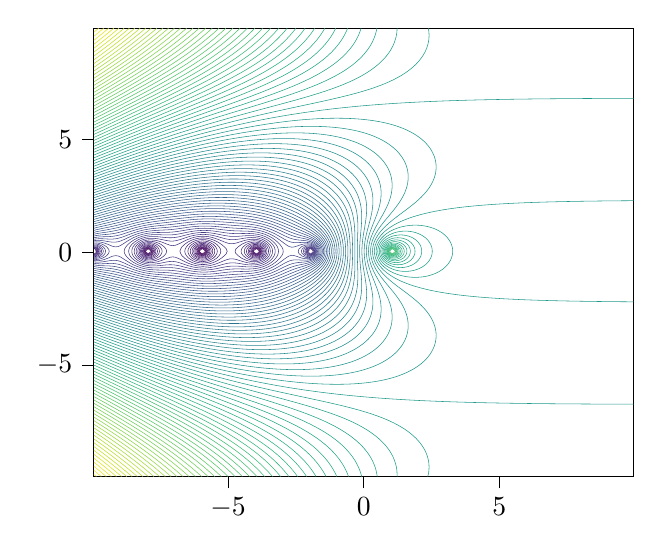
\begin{tikzpicture}

\definecolor{color0}{rgb}{0.269944,0.014625,0.341379}
\definecolor{color1}{rgb}{0.273809,0.031497,0.358853}
\definecolor{color2}{rgb}{0.277018,0.050344,0.375715}
\definecolor{color3}{rgb}{0.279566,0.067836,0.391917}
\definecolor{color4}{rgb}{0.280894,0.078907,0.402329}
\definecolor{color5}{rgb}{0.282327,0.094955,0.417331}
\definecolor{color6}{rgb}{0.283091,0.110553,0.431554}
\definecolor{color7}{rgb}{0.283187,0.125848,0.44496}
\definecolor{color8}{rgb}{0.282884,0.13592,0.453427}
\definecolor{color9}{rgb}{0.281887,0.150881,0.465405}
\definecolor{color10}{rgb}{0.280255,0.165693,0.476498}
\definecolor{color11}{rgb}{0.278012,0.180367,0.486697}
\definecolor{color12}{rgb}{0.276194,0.190074,0.493001}
\definecolor{color13}{rgb}{0.273006,0.20452,0.501721}
\definecolor{color14}{rgb}{0.269308,0.218818,0.509577}
\definecolor{color15}{rgb}{0.265145,0.232956,0.516599}
\definecolor{color16}{rgb}{0.262138,0.242286,0.520837}
\definecolor{color17}{rgb}{0.257322,0.25613,0.526563}
\definecolor{color18}{rgb}{0.252194,0.269783,0.531579}
\definecolor{color19}{rgb}{0.246811,0.283237,0.535941}
\definecolor{color20}{rgb}{0.243113,0.292092,0.538516}
\definecolor{color21}{rgb}{0.237441,0.305202,0.541921}
\definecolor{color22}{rgb}{0.231674,0.318106,0.544834}
\definecolor{color23}{rgb}{0.225863,0.330805,0.547314}
\definecolor{color24}{rgb}{0.221989,0.339161,0.548752}
\definecolor{color25}{rgb}{0.21621,0.351535,0.550627}
\definecolor{color26}{rgb}{0.210503,0.363727,0.552206}
\definecolor{color27}{rgb}{0.204903,0.375746,0.553533}
\definecolor{color28}{rgb}{0.201239,0.38367,0.554294}
\definecolor{color29}{rgb}{0.19586,0.395433,0.555276}
\definecolor{color30}{rgb}{0.190631,0.407061,0.556089}
\definecolor{color31}{rgb}{0.185556,0.41857,0.556753}
\definecolor{color32}{rgb}{0.182256,0.426184,0.55712}
\definecolor{color33}{rgb}{0.177423,0.437527,0.557565}
\definecolor{color34}{rgb}{0.172719,0.448791,0.557885}
\definecolor{color35}{rgb}{0.168126,0.459988,0.558082}
\definecolor{color36}{rgb}{0.165117,0.467423,0.558141}
\definecolor{color37}{rgb}{0.160665,0.47854,0.558115}
\definecolor{color38}{rgb}{0.15627,0.489624,0.557936}
\definecolor{color39}{rgb}{0.151918,0.500685,0.557587}
\definecolor{color40}{rgb}{0.149039,0.508051,0.55725}
\definecolor{color41}{rgb}{0.144759,0.519093,0.556572}
\definecolor{color42}{rgb}{0.140536,0.530132,0.555659}
\definecolor{color43}{rgb}{0.136408,0.541173,0.554483}
\definecolor{color44}{rgb}{0.133743,0.548535,0.553541}
\definecolor{color45}{rgb}{0.129933,0.559582,0.551864}
\definecolor{color46}{rgb}{0.126453,0.570633,0.549841}
\definecolor{color47}{rgb}{0.123463,0.581687,0.547445}
\definecolor{color48}{rgb}{0.121831,0.589055,0.545623}
\definecolor{color49}{rgb}{0.120092,0.600104,0.54253}
\definecolor{color50}{rgb}{0.119423,0.611141,0.538982}
\definecolor{color51}{rgb}{0.120081,0.622161,0.534946}
\definecolor{color52}{rgb}{0.12138,0.629492,0.531973}
\definecolor{color53}{rgb}{0.12478,0.640461,0.527068}
\definecolor{color54}{rgb}{0.130067,0.651384,0.521608}
\definecolor{color55}{rgb}{0.137339,0.662252,0.515571}
\definecolor{color56}{rgb}{0.143303,0.669459,0.511215}
\definecolor{color57}{rgb}{0.153894,0.680203,0.504172}
\definecolor{color58}{rgb}{0.166383,0.690856,0.496502}
\definecolor{color59}{rgb}{0.180653,0.701402,0.488189}
\definecolor{color60}{rgb}{0.19109,0.708366,0.482284}
\definecolor{color61}{rgb}{0.20803,0.718701,0.472873}
\definecolor{color62}{rgb}{0.226397,0.728888,0.462789}
\definecolor{color63}{rgb}{0.24607,0.73891,0.452024}
\definecolor{color64}{rgb}{0.259857,0.745492,0.444467}
\definecolor{color65}{rgb}{0.281477,0.755203,0.432552}
\definecolor{color66}{rgb}{0.304148,0.764704,0.419943}
\definecolor{color67}{rgb}{0.327796,0.77398,0.40664}
\definecolor{color68}{rgb}{0.344074,0.780029,0.397381}
\definecolor{color69}{rgb}{0.369214,0.788888,0.382914}
\definecolor{color70}{rgb}{0.395174,0.797475,0.367757}
\definecolor{color71}{rgb}{0.421908,0.805774,0.35191}
\definecolor{color72}{rgb}{0.440137,0.811138,0.340967}
\definecolor{color73}{rgb}{0.468053,0.818921,0.323998}
\definecolor{color74}{rgb}{0.496615,0.826376,0.306377}
\definecolor{color75}{rgb}{0.525776,0.833491,0.288127}
\definecolor{color76}{rgb}{0.545524,0.838039,0.275626}
\definecolor{color77}{rgb}{0.575563,0.844566,0.256415}
\definecolor{color78}{rgb}{0.606045,0.850733,0.236712}
\definecolor{color79}{rgb}{0.636902,0.856542,0.21662}
\definecolor{color80}{rgb}{0.657642,0.860219,0.203082}
\definecolor{color81}{rgb}{0.688944,0.865448,0.182725}
\definecolor{color82}{rgb}{0.720391,0.87035,0.162603}
\definecolor{color83}{rgb}{0.751884,0.874951,0.143228}
\definecolor{color84}{rgb}{0.772852,0.877868,0.131109}
\definecolor{color85}{rgb}{0.804182,0.882046,0.114965}
\definecolor{color86}{rgb}{0.83527,0.886029,0.102646}
\definecolor{color87}{rgb}{0.866013,0.889868,0.095953}
\definecolor{color88}{rgb}{0.886271,0.892374,0.095374}
\definecolor{color89}{rgb}{0.916242,0.896091,0.100717}
\definecolor{color90}{rgb}{0.945636,0.899815,0.112838}
\definecolor{color91}{rgb}{0.974417,0.90359,0.130215}

\begin{axis}[
tick align=outside,
tick pos=left,
x grid style={white!69.0196078431373!black},
xmin=-9.95, xmax=9.95,
xtick style={color=black},
y grid style={white!69.0196078431373!black},
ymin=-9.95, ymax=9.95,
ytick style={color=black}
]
\path [draw=color0, very thin]
(axis cs:-5.95,-0.0616788019148981)
--(axis cs:-5.97371950722733,-0.0499999999999989)
--(axis cs:-6.05,0.0254614373017482)
--(axis cs:-6.06251722343058,0.0500000000000007)
--(axis cs:-6.05,0.0745385626982532)
--(axis cs:-5.97371950722733,0.15)
--(axis cs:-5.95,0.1616788019149)
--(axis cs:-5.92587611537551,0.15)
--(axis cs:-5.85,0.0761911453862493)
--(axis cs:-5.83652844497252,0.0500000000000007)
--(axis cs:-5.85,0.0238088546137522)
--(axis cs:-5.92587611537551,-0.0499999999999989)
--(axis cs:-5.95,-0.0616788019148981);

\path [draw=color1, very thin]
(axis cs:-5.95,-0.083013950630164)
--(axis cs:-6.01705093949541,-0.0499999999999989)
--(axis cs:-6.05,-0.0174047273025821)
--(axis cs:-6.084383433223,0.0500000000000007)
--(axis cs:-6.05,0.117404727302584)
--(axis cs:-6.01705093949541,0.15)
--(axis cs:-5.95,0.183013950630165)
--(axis cs:-5.88180595562762,0.15)
--(axis cs:-5.85,0.119060604339684)
--(axis cs:-5.81447831059417,0.0500000000000007)
--(axis cs:-5.85,-0.0190606043396829)
--(axis cs:-5.88180595562762,-0.0499999999999989)
--(axis cs:-5.95,-0.083013950630164);

\path [draw=color2, very thin]
(axis cs:-7.95,-0.0554889205752715)
--(axis cs:-7.96034888348616,-0.0499999999999989)
--(axis cs:-8.05,0.0455643627850008)
--(axis cs:-8.05217916570908,0.0500000000000007)
--(axis cs:-8.05,0.0544356372150006)
--(axis cs:-7.96034888348616,0.15)
--(axis cs:-7.95,0.155488920575273)
--(axis cs:-7.9376576080165,0.15)
--(axis cs:-7.85,0.0716494490511935)
--(axis cs:-7.83838241011169,0.0500000000000007)
--(axis cs:-7.85,0.0283505509488079)
--(axis cs:-7.9376576080165,-0.0499999999999989)
--(axis cs:-7.95,-0.0554889205752715);

\path [draw=color2, very thin]
(axis cs:-6.05,-0.0576769344782492)
--(axis cs:-6.05796797338035,-0.0499999999999989)
--(axis cs:-6.10624964301542,0.0500000000000007)
--(axis cs:-6.05796797338035,0.15)
--(axis cs:-6.05,0.157676934478251)
--(axis cs:-5.95,0.204349099345431)
--(axis cs:-5.85,0.158917925451911)
--(axis cs:-5.84062610951257,0.15)
--(axis cs:-5.79242817621582,0.0500000000000007)
--(axis cs:-5.84062610951257,-0.0499999999999989)
--(axis cs:-5.85,-0.0589179254519098)
--(axis cs:-5.95,-0.10434909934543)
--(axis cs:-6.05,-0.0576769344782492);

\path [draw=color2, very thin]
(axis cs:-3.95,-0.0614041513540448)
--(axis cs:-3.97600269199246,-0.0499999999999989)
--(axis cs:-4.05,0.0151619138470325)
--(axis cs:-4.06877933895404,0.0500000000000007)
--(axis cs:-4.05,0.0848380861529689)
--(axis cs:-3.97600269199246,0.15)
--(axis cs:-3.95,0.161404151354046)
--(axis cs:-3.92891679385758,0.15)
--(axis cs:-3.85,0.0642737862891873)
--(axis cs:-3.8430763253073,0.0500000000000007)
--(axis cs:-3.85,0.0357262137108141)
--(axis cs:-3.92891679385758,-0.0499999999999989)
--(axis cs:-3.95,-0.0614041513540448);

\path [draw=color3, very thin]
(axis cs:-7.95,-0.0768061470538092)
--(axis cs:-8.00054066437442,-0.0499999999999989)
--(axis cs:-8.05,0.00272159540922527)
--(axis cs:-8.0732272102227,0.0500000000000007)
--(axis cs:-8.05,0.0972784045907762)
--(axis cs:-8.00054066437442,0.15)
--(axis cs:-7.95,0.176806147053811)
--(axis cs:-7.88972367244737,0.15)
--(axis cs:-7.85,0.114493993249558)
--(axis cs:-7.81539104703953,0.0500000000000007)
--(axis cs:-7.85,-0.0144939932495564)
--(axis cs:-7.88972367244737,-0.0499999999999989)
--(axis cs:-7.95,-0.0768061470538092);

\path [draw=color3, very thin]
(axis cs:-6.05,-0.0897170669208681)
--(axis cs:-6.09122277360417,-0.0499999999999989)
--(axis cs:-6.12811585280783,0.0500000000000007)
--(axis cs:-6.09122277360417,0.15)
--(axis cs:-6.05,0.18971706692087)
--(axis cs:-5.95,0.225684248060697)
--(axis cs:-5.85,0.190963575983454)
--(axis cs:-5.80694199538747,0.15)
--(axis cs:-5.77037804183747,0.0500000000000007)
--(axis cs:-5.80694199538747,-0.0499999999999989)
--(axis cs:-5.85,-0.0909635759834528)
--(axis cs:-5.95,-0.125684248060696)
--(axis cs:-6.05,-0.0897170669208681);

\path [draw=color3, very thin]
(axis cs:-3.95,-0.0827782326034613)
--(axis cs:-4.02473789675219,-0.0499999999999989)
--(axis cs:-4.05,-0.0277542313395948)
--(axis cs:-4.09191312516497,0.0500000000000007)
--(axis cs:-4.05,0.127754231339596)
--(axis cs:-4.02473789675219,0.15)
--(axis cs:-3.95,0.182778232603463)
--(axis cs:-3.88940187099343,0.15)
--(axis cs:-3.85,0.107198296480662)
--(axis cs:-3.8222552664174,0.0500000000000007)
--(axis cs:-3.85,-0.00719829648066091)
--(axis cs:-3.88940187099343,-0.0499999999999989)
--(axis cs:-3.95,-0.0827782326034613);

\path [draw=color4, very thin]
(axis cs:-7.95,-0.0981233735323467)
--(axis cs:-8.04073244526268,-0.0499999999999989)
--(axis cs:-8.05,-0.04012117196655)
--(axis cs:-8.09427525473631,0.0500000000000007)
--(axis cs:-8.05,0.140121171966551)
--(axis cs:-8.04073244526268,0.15)
--(axis cs:-7.95,0.198123373532348)
--(axis cs:-7.85,0.155481726940005)
--(axis cs:-7.84384570182977,0.15)
--(axis cs:-7.79239968396736,0.0500000000000007)
--(axis cs:-7.84384570182977,-0.0499999999999989)
--(axis cs:-7.85,-0.0554817269400031)
--(axis cs:-7.95,-0.0981233735323467);

\path [draw=color4, very thin]
(axis cs:-6.05,-0.121757199363487)
--(axis cs:-6.12447757382799,-0.0499999999999989)
--(axis cs:-6.14998206260025,0.0500000000000007)
--(axis cs:-6.12447757382799,0.15)
--(axis cs:-6.05,0.221757199363488)
--(axis cs:-5.95,0.247019396775963)
--(axis cs:-5.85,0.223009226514997)
--(axis cs:-5.77325788126238,0.15)
--(axis cs:-5.75,0.0598957625485396)
--(axis cs:-5.74705184174834,0.0500000000000007)
--(axis cs:-5.75,0.0401042374514619)
--(axis cs:-5.77325788126238,-0.0499999999999989)
--(axis cs:-5.85,-0.123009226514995)
--(axis cs:-5.95,-0.147019396775962)
--(axis cs:-6.05,-0.121757199363487);

\path [draw=color4, very thin]
(axis cs:-4.05,-0.0654723515611623)
--(axis cs:-4.06747230616003,-0.0499999999999989)
--(axis cs:-4.1150469113759,0.0500000000000007)
--(axis cs:-4.06747230616003,0.15)
--(axis cs:-4.05,0.165472351561164)
--(axis cs:-3.95,0.204152313852879)
--(axis cs:-3.85,0.150091946462213)
--(axis cs:-3.84991159723322,0.15)
--(axis cs:-3.8014342075275,0.0500000000000007)
--(axis cs:-3.84991159723322,-0.0499999999999989)
--(axis cs:-3.85,-0.0500919464622114)
--(axis cs:-3.95,-0.104152313852878)
--(axis cs:-4.05,-0.0654723515611623);

\path [draw=color5, very thin]
(axis cs:-6.05,-0.154895609381335)
--(axis cs:-6.05779245392741,-0.149999999999999)
--(axis cs:-6.15,-0.0642219238189379)
--(axis cs:-6.16048435630016,-0.0499999999999989)
--(axis cs:-6.18828875783607,0.0500000000000007)
--(axis cs:-6.16048435630016,0.15)
--(axis cs:-6.15,0.164221923818939)
--(axis cs:-6.05779245392741,0.25)
--(axis cs:-6.05,0.254895609381337)
--(axis cs:-5.95,0.280589077732756)
--(axis cs:-5.85,0.256518152410462)
--(axis cs:-5.83935677166,0.25)
--(axis cs:-5.75,0.168944713469992)
--(axis cs:-5.73580244846552,0.15)
--(axis cs:-5.70817403802113,0.0500000000000007)
--(axis cs:-5.73580244846552,-0.0499999999999989)
--(axis cs:-5.75,-0.0689447134699902)
--(axis cs:-5.83935677166,-0.149999999999999)
--(axis cs:-5.85,-0.15651815241046)
--(axis cs:-5.95,-0.180589077732755)
--(axis cs:-6.05,-0.154895609381335);

\path [draw=color5, very thin]
(axis cs:-8.05,-0.0746220752685762)
--(axis cs:-8.07415891047256,-0.0499999999999989)
--(axis cs:-8.11532329924993,0.0500000000000007)
--(axis cs:-8.07415891047256,0.15)
--(axis cs:-8.05,0.174622075268578)
--(axis cs:-7.95,0.219440600010886)
--(axis cs:-7.85,0.187485664213758)
--(axis cs:-7.80791509551545,0.15)
--(axis cs:-7.7694083208952,0.0500000000000007)
--(axis cs:-7.80791509551545,-0.0499999999999989)
--(axis cs:-7.85,-0.0874856642137566)
--(axis cs:-7.95,-0.119440600010884)
--(axis cs:-8.05,-0.0746220752685762);

\path [draw=color5, very thin]
(axis cs:-4.05,-0.0975962794990519)
--(axis cs:-4.10374856977611,-0.0499999999999989)
--(axis cs:-4.13818069758683,0.0500000000000007)
--(axis cs:-4.10374856977611,0.15)
--(axis cs:-4.05,0.197596279499053)
--(axis cs:-3.95,0.225526395102296)
--(axis cs:-3.85,0.182229914095738)
--(axis cs:-3.81901225440963,0.15)
--(axis cs:-3.78061314863759,0.0500000000000007)
--(axis cs:-3.81901225440963,-0.0499999999999989)
--(axis cs:-3.85,-0.0822299140957368)
--(axis cs:-3.95,-0.125526395102294)
--(axis cs:-4.05,-0.0975962794990519);

\path [draw=color6, very thin]
(axis cs:-6.05,-0.196202500897398)
--(axis cs:-6.12354158216679,-0.149999999999999)
--(axis cs:-6.15,-0.125386481072376)
--(axis cs:-6.20557467033576,-0.0499999999999989)
--(axis cs:-6.22660895068644,0.0500000000000007)
--(axis cs:-6.20557467033576,0.15)
--(axis cs:-6.15,0.225386481072377)
--(axis cs:-6.12354158216679,0.25)
--(axis cs:-6.05,0.296202500897399)
--(axis cs:-5.95,0.316145530100538)
--(axis cs:-5.85,0.297840311650708)
--(axis cs:-5.77188348343346,0.25)
--(axis cs:-5.75,0.230149551208916)
--(axis cs:-5.68993430486259,0.15)
--(axis cs:-5.66929623429393,0.0500000000000007)
--(axis cs:-5.68993430486259,-0.0499999999999989)
--(axis cs:-5.75,-0.130149551208914)
--(axis cs:-5.77188348343346,-0.149999999999999)
--(axis cs:-5.85,-0.197840311650706)
--(axis cs:-5.95,-0.216145530100537)
--(axis cs:-6.05,-0.196202500897398);

\path [draw=color6, very thin]
(axis cs:-8.05,-0.106623039476334)
--(axis cs:-8.1055579059227,-0.0499999999999989)
--(axis cs:-8.13637134376354,0.0500000000000007)
--(axis cs:-8.1055579059227,0.15)
--(axis cs:-8.05,0.206623039476335)
--(axis cs:-7.95,0.240757826489423)
--(axis cs:-7.85,0.219489601487511)
--(axis cs:-7.77198448920113,0.15)
--(axis cs:-7.75,0.0702999124724558)
--(axis cs:-7.74346213684277,0.0500000000000007)
--(axis cs:-7.75,0.0297000875275456)
--(axis cs:-7.77198448920113,-0.0499999999999989)
--(axis cs:-7.85,-0.11948960148751)
--(axis cs:-7.95,-0.140757826489422)
--(axis cs:-8.05,-0.106623039476334);

\path [draw=color6, very thin]
(axis cs:-4.05,-0.129720207436941)
--(axis cs:-4.14002483339219,-0.0499999999999989)
--(axis cs:-4.15,-0.0140112962877381)
--(axis cs:-4.17068733443323,0.0500000000000007)
--(axis cs:-4.15,0.11401129628774)
--(axis cs:-4.14002483339219,0.15)
--(axis cs:-4.05,0.229720207436943)
--(axis cs:-3.95,0.246900476351712)
--(axis cs:-3.85,0.214367881729263)
--(axis cs:-3.78811291158603,0.15)
--(axis cs:-3.75979208974769,0.0500000000000007)
--(axis cs:-3.78811291158603,-0.0499999999999989)
--(axis cs:-3.85,-0.114367881729262)
--(axis cs:-3.95,-0.146900476351711)
--(axis cs:-4.05,-0.129720207436941);

\path [draw=color7, very thin]
(axis cs:-9.89194065086012,0.0919406508601264)
--(axis cs:-9.85,0.0570202793462688)
--(axis cs:-9.84610262661879,0.0500000000000007)
--(axis cs:-9.85,0.0429797206537326)
--(axis cs:-9.89194065086012,0.00805934913987505);

\path [draw=color7, very thin]
(axis cs:-5.95,-0.252313365587047)
--(axis cs:-5.96366643618318,-0.25)
--(axis cs:-6.05,-0.23750939241346)
--(axis cs:-6.15,-0.184519326534912)
--(axis cs:-6.18910954040618,-0.149999999999999)
--(axis cs:-6.25,-0.0515603846329993)
--(axis cs:-6.2509053407131,-0.0499999999999989)
--(axis cs:-6.27192424321625,0.0500000000000007)
--(axis cs:-6.2509053407131,0.15)
--(axis cs:-6.25,0.151560384633001)
--(axis cs:-6.18910954040618,0.25)
--(axis cs:-6.15,0.284519326534913)
--(axis cs:-6.05,0.337509392413462)
--(axis cs:-5.96366643618318,0.350000000000001)
--(axis cs:-5.95,0.352313365587049)
--(axis cs:-5.93456579917704,0.350000000000001)
--(axis cs:-5.85,0.339162470890954)
--(axis cs:-5.75,0.289070393172516)
--(axis cs:-5.70464767505804,0.25)
--(axis cs:-5.65,0.163711078723845)
--(axis cs:-5.64187621064696,0.15)
--(axis cs:-5.62106395888266,0.0500000000000007)
--(axis cs:-5.64187621064696,-0.0499999999999989)
--(axis cs:-5.65,-0.0637110787238439)
--(axis cs:-5.70464767505804,-0.149999999999999)
--(axis cs:-5.75,-0.189070393172514)
--(axis cs:-5.85,-0.239162470890953)
--(axis cs:-5.93456579917704,-0.25)
--(axis cs:-5.95,-0.252313365587047);

\path [draw=color7, very thin]
(axis cs:-7.95,-0.170093926546164)
--(axis cs:-8.01144097017469,-0.149999999999999)
--(axis cs:-8.05,-0.138624003684092)
--(axis cs:-8.13695690137283,-0.0499999999999989)
--(axis cs:-8.15,0.00409566012624714)
--(axis cs:-8.16265752378445,0.0500000000000007)
--(axis cs:-8.15,0.0959043398737543)
--(axis cs:-8.13695690137283,0.15)
--(axis cs:-8.05,0.238624003684093)
--(axis cs:-8.01144097017469,0.25)
--(axis cs:-7.95,0.270093926546165)
--(axis cs:-7.85,0.2519230145846)
--(axis cs:-7.84640074991969,0.25)
--(axis cs:-7.75,0.173695148573658)
--(axis cs:-7.73051256071532,0.15)
--(axis cs:-7.70151052752858,0.0500000000000007)
--(axis cs:-7.73051256071532,-0.0499999999999989)
--(axis cs:-7.75,-0.0736951485736566)
--(axis cs:-7.84640074991969,-0.149999999999999)
--(axis cs:-7.85,-0.151923014584599)
--(axis cs:-7.95,-0.170093926546164);

\path [draw=color7, very thin]
(axis cs:-4.05,-0.165315555792599)
--(axis cs:-4.07901240953251,-0.149999999999999)
--(axis cs:-4.15,-0.0945574970285402)
--(axis cs:-4.18675666480895,-0.0499999999999989)
--(axis cs:-4.21298501063366,0.0500000000000007)
--(axis cs:-4.18675666480895,0.15)
--(axis cs:-4.15,0.194557497028542)
--(axis cs:-4.07901240953251,0.25)
--(axis cs:-4.05,0.265315555792601)
--(axis cs:-3.95,0.28055451974754)
--(axis cs:-3.86128175676926,0.25)
--(axis cs:-3.85,0.246505849362789)
--(axis cs:-3.75721356876243,0.15)
--(axis cs:-3.75,0.119409443070426)
--(axis cs:-3.73138891000652,0.0500000000000007)
--(axis cs:-3.75,-0.0194094430704242)
--(axis cs:-3.75721356876243,-0.0499999999999989)
--(axis cs:-3.85,-0.146505849362787)
--(axis cs:-3.86128175676926,-0.149999999999999)
--(axis cs:-3.95,-0.180554519747538)
--(axis cs:-4.05,-0.165315555792599);

\path [draw=color8, very thin]
(axis cs:-9.95,0.166472146974723)
--(axis cs:-9.91023156336006,0.15)
--(axis cs:-9.85,0.0998503593468648)
--(axis cs:-9.82232510930418,0.0500000000000007)
--(axis cs:-9.85,0.000149640653136583)
--(axis cs:-9.91023156336006,-0.0499999999999989)
--(axis cs:-9.95,-0.0664721469747214);

\path [draw=color8, very thin]
(axis cs:-6.05,-0.286305554283243)
--(axis cs:-6.13392953862202,-0.25)
--(axis cs:-6.15,-0.242284014513793)
--(axis cs:-6.25,-0.155794176590821)
--(axis cs:-6.25535656338563,-0.149999999999999)
--(axis cs:-6.31229339556192,-0.0499999999999989)
--(axis cs:-6.32819948941999,0.0500000000000007)
--(axis cs:-6.31229339556192,0.15)
--(axis cs:-6.25535656338563,0.25)
--(axis cs:-6.25,0.255794176590822)
--(axis cs:-6.15,0.342284014513794)
--(axis cs:-6.13392953862202,0.350000000000001)
--(axis cs:-6.05,0.386305554283244)
--(axis cs:-5.95,0.40064234360898)
--(axis cs:-5.85,0.388418293501652)
--(axis cs:-5.75678502821601,0.350000000000001)
--(axis cs:-5.75,0.34689489827005)
--(axis cs:-5.65,0.265504561292106)
--(axis cs:-5.63527853057338,0.25)
--(axis cs:-5.57907990745246,0.15)
--(axis cs:-5.56361352157036,0.0500000000000007)
--(axis cs:-5.57907990745246,-0.0499999999999989)
--(axis cs:-5.63527853057338,-0.149999999999999)
--(axis cs:-5.65,-0.165504561292104)
--(axis cs:-5.75,-0.246894898270049)
--(axis cs:-5.75678502821601,-0.25)
--(axis cs:-5.85,-0.288418293501651)
--(axis cs:-5.95,-0.300642343608978)
--(axis cs:-6.05,-0.286305554283243);

\path [draw=color8, very thin]
(axis cs:-8.05,-0.176552975388531)
--(axis cs:-8.0879447994704,-0.149999999999999)
--(axis cs:-8.15,-0.0856760318949347)
--(axis cs:-8.17442932254557,-0.0499999999999989)
--(axis cs:-8.19856562214716,0.0500000000000007)
--(axis cs:-8.17442932254557,0.15)
--(axis cs:-8.15,0.185676031894936)
--(axis cs:-8.0879447994704,0.25)
--(axis cs:-8.05,0.276552975388532)
--(axis cs:-7.95,0.305567624604819)
--(axis cs:-7.85,0.293129871572987)
--(axis cs:-7.76927508248453,0.25)
--(axis cs:-7.75,0.234743040832799)
--(axis cs:-7.68030535943278,0.15)
--(axis cs:-7.65955891821438,0.0500000000000007)
--(axis cs:-7.68030535943278,-0.0499999999999989)
--(axis cs:-7.75,-0.134743040832798)
--(axis cs:-7.76927508248453,-0.149999999999999)
--(axis cs:-7.85,-0.193129871572985)
--(axis cs:-7.95,-0.205567624604817)
--(axis cs:-8.05,-0.176552975388531);

\path [draw=color8, very thin]
(axis cs:-4.15,-0.155695451225293)
--(axis cs:-4.15762727776692,-0.149999999999999)
--(axis cs:-4.23745395936811,-0.0499999999999989)
--(axis cs:-4.25,0.0164592952619746)
--(axis cs:-4.25812816755324,0.0500000000000007)
--(axis cs:-4.25,0.0835407047380269)
--(axis cs:-4.23745395936811,0.15)
--(axis cs:-4.15762727776692,0.25)
--(axis cs:-4.15,0.255695451225294)
--(axis cs:-4.05,0.306854747556288)
--(axis cs:-3.95,0.316291351351085)
--(axis cs:-3.85,0.287057677043682)
--(axis cs:-3.79904558373476,0.25)
--(axis cs:-3.75,0.197188506388138)
--(axis cs:-3.71876341157284,0.15)
--(axis cs:-3.6962539308654,0.0500000000000007)
--(axis cs:-3.71876341157284,-0.0499999999999989)
--(axis cs:-3.75,-0.0971885063881368)
--(axis cs:-3.79904558373476,-0.149999999999999)
--(axis cs:-3.85,-0.18705767704368)
--(axis cs:-3.95,-0.216291351351084)
--(axis cs:-4.05,-0.206854747556287)
--(axis cs:-4.15,-0.155695451225293);

\path [draw=color9, very thin]
(axis cs:-9.95,0.18777888107606)
--(axis cs:-9.85879106162017,0.15)
--(axis cs:-9.85,0.142680439347461)
--(axis cs:-9.79854759198956,0.0500000000000007)
--(axis cs:-9.85,-0.0426804393474592)
--(axis cs:-9.85879106162017,-0.0499999999999989)
--(axis cs:-9.95,-0.0877788810760585);

\path [draw=color9, very thin]
(axis cs:-6.15,-0.304426729430029)
--(axis cs:-6.23680347981279,-0.25)
--(axis cs:-6.25,-0.239035436952402)
--(axis cs:-6.33231091236643,-0.149999999999999)
--(axis cs:-6.35,-0.11266194395064)
--(axis cs:-6.38143383248877,-0.0499999999999989)
--(axis cs:-6.39723010791386,0.0500000000000007)
--(axis cs:-6.38143383248877,0.15)
--(axis cs:-6.35,0.212661943950641)
--(axis cs:-6.33231091236643,0.25)
--(axis cs:-6.25,0.339035436952403)
--(axis cs:-6.23680347981279,0.350000000000001)
--(axis cs:-6.15,0.40442672943003)
--(axis cs:-6.05,0.438347989590872)
--(axis cs:-5.95,0.44897132163091)
--(axis cs:-5.85,0.440494596706953)
--(axis cs:-5.75,0.409538017067231)
--(axis cs:-5.65133387294024,0.350000000000001)
--(axis cs:-5.65,0.348932695498458)
--(axis cs:-5.55606411722112,0.25)
--(axis cs:-5.55,0.237521281683802)
--(axis cs:-5.50496203567762,0.15)
--(axis cs:-5.48954530050608,0.0500000000000007)
--(axis cs:-5.50496203567762,-0.0499999999999989)
--(axis cs:-5.55,-0.1375212816838)
--(axis cs:-5.55606411722112,-0.149999999999999)
--(axis cs:-5.65,-0.248932695498456)
--(axis cs:-5.65133387294024,-0.25)
--(axis cs:-5.75,-0.30953801706723)
--(axis cs:-5.85,-0.340494596706951)
--(axis cs:-5.95,-0.348971321630909)
--(axis cs:-6.05,-0.338347989590871)
--(axis cs:-6.15,-0.304426729430029);

\path [draw=color9, very thin]
(axis cs:-3.95,-0.252769333782867)
--(axis cs:-4.00947920375171,-0.25)
--(axis cs:-4.05,-0.248393939319974)
--(axis cs:-4.15,-0.213894721951508)
--(axis cs:-4.23556702057247,-0.149999999999999)
--(axis cs:-4.25,-0.13025179062406)
--(axis cs:-4.30419131942477,-0.0499999999999989)
--(axis cs:-4.32320917842291,0.0500000000000007)
--(axis cs:-4.30419131942477,0.15)
--(axis cs:-4.25,0.230251790624062)
--(axis cs:-4.23556702057247,0.25)
--(axis cs:-4.15,0.313894721951509)
--(axis cs:-4.05,0.348393939319976)
--(axis cs:-4.00947920375171,0.350000000000001)
--(axis cs:-3.95,0.352769333782869)
--(axis cs:-3.94005345696263,0.350000000000001)
--(axis cs:-3.85,0.328635879612031)
--(axis cs:-3.75,0.258292677116795)
--(axis cs:-3.74193997031408,0.25)
--(axis cs:-3.67801363274113,0.15)
--(axis cs:-3.66111895172429,0.0500000000000007)
--(axis cs:-3.67801363274113,-0.0499999999999989)
--(axis cs:-3.74193997031408,-0.149999999999999)
--(axis cs:-3.75,-0.158292677116794)
--(axis cs:-3.85,-0.22863587961203)
--(axis cs:-3.94005345696263,-0.25)
--(axis cs:-3.95,-0.252769333782867);

\path [draw=color9, very thin]
(axis cs:-8.05,-0.217751624495453)
--(axis cs:-8.14681859632137,-0.149999999999999)
--(axis cs:-8.15,-0.146702282693355)
--(axis cs:-8.21621732096681,-0.0499999999999989)
--(axis cs:-8.23447372050986,0.0500000000000007)
--(axis cs:-8.21621732096681,0.15)
--(axis cs:-8.15,0.246702282693356)
--(axis cs:-8.14681859632137,0.25)
--(axis cs:-8.05,0.317751624495454)
--(axis cs:-7.95,0.341041322663472)
--(axis cs:-7.85,0.334336728561373)
--(axis cs:-7.75,0.29319844961541)
--(axis cs:-7.69237019935332,0.25)
--(axis cs:-7.65,0.191819705137399)
--(axis cs:-7.62170917795085,0.15)
--(axis cs:-7.60016082486392,0.0500000000000007)
--(axis cs:-7.62170917795085,-0.0499999999999989)
--(axis cs:-7.65,-0.091819705137398)
--(axis cs:-7.69237019935332,-0.149999999999999)
--(axis cs:-7.75,-0.193198449615408)
--(axis cs:-7.85,-0.234336728561372)
--(axis cs:-7.95,-0.241041322663471)
--(axis cs:-8.05,-0.217751624495453);

\path [draw=color10, very thin]
(axis cs:-2.00150665028766,0.00150665028766081)
--(axis cs:-2.05,0.034589083656708)
--(axis cs:-2.05923396569948,0.0500000000000007)
--(axis cs:-2.05,0.0654109163432935)
--(axis cs:-2.00150665028766,0.0984933497123406);

\path [draw=color10, very thin]
(axis cs:-9.95,0.209085615177397)
--(axis cs:-9.85,0.176514479010136)
--(axis cs:-9.81858693833458,0.15)
--(axis cs:-9.77477007467494,0.0500000000000007)
--(axis cs:-9.81858693833458,-0.0499999999999989)
--(axis cs:-9.85,-0.0765144790101342)
--(axis cs:-9.95,-0.109085615177396);

\path [draw=color10, very thin]
(axis cs:-6.15,-0.36911886765476)
--(axis cs:-6.19144956682026,-0.35)
--(axis cs:-6.25,-0.31912770508016)
--(axis cs:-6.34008164877297,-0.25)
--(axis cs:-6.35,-0.238957252667486)
--(axis cs:-6.42307210638086,-0.149999999999999)
--(axis cs:-6.45,-0.0858399412531062)
--(axis cs:-6.46695896174557,-0.0499999999999989)
--(axis cs:-6.48245458240204,0.0500000000000007)
--(axis cs:-6.46695896174557,0.15)
--(axis cs:-6.45,0.185839941253108)
--(axis cs:-6.42307210638086,0.25)
--(axis cs:-6.35,0.338957252667487)
--(axis cs:-6.34008164877297,0.350000000000001)
--(axis cs:-6.25,0.419127705080162)
--(axis cs:-6.19144956682026,0.450000000000001)
--(axis cs:-6.15,0.469118867654761)
--(axis cs:-6.05,0.498216343152141)
--(axis cs:-5.95,0.508286449132104)
--(axis cs:-5.85,0.500836853168751)
--(axis cs:-5.75,0.474911911439595)
--(axis cs:-5.69261961241998,0.450000000000001)
--(axis cs:-5.65,0.42883198435273)
--(axis cs:-5.55,0.356217701128544)
--(axis cs:-5.54243990507757,0.350000000000001)
--(axis cs:-5.45931483638367,0.25)
--(axis cs:-5.45,0.228424217532762)
--(axis cs:-5.41175642334594,0.15)
--(axis cs:-5.39666683323058,0.0500000000000007)
--(axis cs:-5.41175642334594,-0.0499999999999989)
--(axis cs:-5.45,-0.128424217532761)
--(axis cs:-5.45931483638367,-0.149999999999999)
--(axis cs:-5.54243990507757,-0.25)
--(axis cs:-5.55,-0.256217701128543)
--(axis cs:-5.65,-0.328831984352729)
--(axis cs:-5.69261961241998,-0.35)
--(axis cs:-5.75,-0.374911911439593)
--(axis cs:-5.85,-0.40083685316875)
--(axis cs:-5.95,-0.408286449132103)
--(axis cs:-6.05,-0.398216343152139)
--(axis cs:-6.15,-0.36911886765476);

\path [draw=color10, very thin]
(axis cs:-8.05,-0.261253975561079)
--(axis cs:-8.07153910770537,-0.25)
--(axis cs:-8.15,-0.204449169762887)
--(axis cs:-8.20554260492309,-0.149999999999999)
--(axis cs:-8.25,-0.0701920957446121)
--(axis cs:-8.26063187294976,-0.0499999999999989)
--(axis cs:-8.27911005660063,0.0500000000000007)
--(axis cs:-8.26063187294976,0.15)
--(axis cs:-8.25,0.170192095744614)
--(axis cs:-8.20554260492309,0.25)
--(axis cs:-8.15,0.304449169762888)
--(axis cs:-8.07153910770537,0.350000000000001)
--(axis cs:-8.05,0.36125397556108)
--(axis cs:-7.95,0.385964369214808)
--(axis cs:-7.85,0.382123077518516)
--(axis cs:-7.75,0.350857850995226)
--(axis cs:-7.74822079470029,0.350000000000001)
--(axis cs:-7.65,0.28719575330515)
--(axis cs:-7.60812964416967,0.25)
--(axis cs:-7.55033874863118,0.15)
--(axis cs:-7.55,0.147914784926123)
--(axis cs:-7.5291281114999,0.0500000000000007)
--(axis cs:-7.55,-0.0479147849261213)
--(axis cs:-7.55033874863118,-0.0499999999999989)
--(axis cs:-7.60812964416967,-0.149999999999999)
--(axis cs:-7.65,-0.187195753305149)
--(axis cs:-7.74822079470029,-0.25)
--(axis cs:-7.75,-0.250857850995225)
--(axis cs:-7.85,-0.282123077518515)
--(axis cs:-7.95,-0.285964369214807)
--(axis cs:-8.05,-0.261253975561079);

\path [draw=color10, very thin]
(axis cs:-4.15,-0.274120597085246)
--(axis cs:-4.20036314982982,-0.25)
--(axis cs:-4.25,-0.218531441509079)
--(axis cs:-4.32690844473627,-0.149999999999999)
--(axis cs:-4.35,-0.109796544454163)
--(axis cs:-4.38669411421303,-0.0499999999999989)
--(axis cs:-4.40543192698069,0.0500000000000007)
--(axis cs:-4.38669411421303,0.15)
--(axis cs:-4.35,0.209796544454165)
--(axis cs:-4.32690844473627,0.25)
--(axis cs:-4.25,0.31853144150908)
--(axis cs:-4.20036314982982,0.350000000000001)
--(axis cs:-4.15,0.374120597085247)
--(axis cs:-4.05,0.400527005341762)
--(axis cs:-3.95,0.401565333584793)
--(axis cs:-3.85,0.375595006488707)
--(axis cs:-3.80403792020796,0.350000000000001)
--(axis cs:-3.75,0.316645758749699)
--(axis cs:-3.68522395887386,0.25)
--(axis cs:-3.65,0.183477286454716)
--(axis cs:-3.6333122585256,0.15)
--(axis cs:-3.61618271897651,0.0500000000000007)
--(axis cs:-3.6333122585256,-0.0499999999999989)
--(axis cs:-3.65,-0.0834772864547142)
--(axis cs:-3.68522395887386,-0.149999999999999)
--(axis cs:-3.75,-0.216645758749698)
--(axis cs:-3.80403792020796,-0.25)
--(axis cs:-3.85,-0.275595006488705)
--(axis cs:-3.95,-0.301565333584792)
--(axis cs:-4.05,-0.300527005341761)
--(axis cs:-4.15,-0.274120597085246);

\path [draw=color11, very thin]
(axis cs:-1.86182115613965,0.0381788438603479)
--(axis cs:-1.92947125557866,-0.0499999999999989)
--(axis cs:-1.95,-0.0633480817364349)
--(axis cs:-1.98918079306604,-0.0499999999999989)
--(axis cs:-2.05,-0.00850879815714159)
--(axis cs:-2.08505750230979,0.0500000000000007)
--(axis cs:-2.05,0.108508798157143)
--(axis cs:-1.98918079306604,0.15)
--(axis cs:-1.95,0.163348081736436)
--(axis cs:-1.92947125557866,0.15)
--(axis cs:-1.86182115613965,0.0618211561396535);

\path [draw=color11, very thin]
(axis cs:-9.95,0.230392349278734)
--(axis cs:-9.85,0.208494221295723)
--(axis cs:-9.78069889927195,0.15)
--(axis cs:-9.75099255736033,0.0500000000000007)
--(axis cs:-9.78069889927195,-0.0499999999999989)
--(axis cs:-9.85,-0.108494221295722)
--(axis cs:-9.95,-0.130392349278733);

\path [draw=color11, very thin]
(axis cs:-6.05,-0.461823898362194)
--(axis cs:-6.10078635705645,-0.449999999999999)
--(axis cs:-6.15,-0.438764815968129)
--(axis cs:-6.25,-0.399839407841195)
--(axis cs:-6.33760359868019,-0.35)
--(axis cs:-6.35,-0.341258238956722)
--(axis cs:-6.45,-0.257099627317423)
--(axis cs:-6.458037156077,-0.25)
--(axis cs:-6.53562006210152,-0.149999999999999)
--(axis cs:-6.55,-0.115034652840753)
--(axis cs:-6.58167478702532,-0.0499999999999989)
--(axis cs:-6.59717209842351,0.0500000000000007)
--(axis cs:-6.58167478702532,0.15)
--(axis cs:-6.55,0.215034652840754)
--(axis cs:-6.53562006210152,0.25)
--(axis cs:-6.458037156077,0.350000000000001)
--(axis cs:-6.45,0.357099627317425)
--(axis cs:-6.35,0.441258238956723)
--(axis cs:-6.33760359868019,0.450000000000001)
--(axis cs:-6.25,0.499839407841197)
--(axis cs:-6.15,0.538764815968131)
--(axis cs:-6.10078635705645,0.550000000000001)
--(axis cs:-6.05,0.561823898362195)
--(axis cs:-5.95,0.570728424007102)
--(axis cs:-5.85,0.564896393069459)
--(axis cs:-5.7765562598438,0.550000000000001)
--(axis cs:-5.75,0.544713804134817)
--(axis cs:-5.65,0.51006257563107)
--(axis cs:-5.55,0.457298210574017)
--(axis cs:-5.53786112241686,0.450000000000001)
--(axis cs:-5.45,0.381478533673465)
--(axis cs:-5.4128196629215,0.350000000000001)
--(axis cs:-5.35,0.269504381686465)
--(axis cs:-5.33337407693961,0.25)
--(axis cs:-5.28435446042751,0.15)
--(axis cs:-5.2693880072341,0.0500000000000007)
--(axis cs:-5.28435446042751,-0.0499999999999989)
--(axis cs:-5.33337407693961,-0.149999999999999)
--(axis cs:-5.35,-0.169504381686464)
--(axis cs:-5.4128196629215,-0.25)
--(axis cs:-5.45,-0.281478533673464)
--(axis cs:-5.53786112241686,-0.35)
--(axis cs:-5.55,-0.357298210574016)
--(axis cs:-5.65,-0.410062575631069)
--(axis cs:-5.75,-0.444713804134816)
--(axis cs:-5.7765562598438,-0.449999999999999)
--(axis cs:-5.85,-0.464896393069458)
--(axis cs:-5.95,-0.4707284240071)
--(axis cs:-6.05,-0.461823898362194);

\path [draw=color11, very thin]
(axis cs:-4.05,-0.353703519164985)
--(axis cs:-4.07321218490228,-0.35)
--(axis cs:-4.15,-0.337658282659731)
--(axis cs:-4.25,-0.300520292800258)
--(axis cs:-4.33639448857057,-0.25)
--(axis cs:-4.35,-0.238457907745857)
--(axis cs:-4.44226798194645,-0.149999999999999)
--(axis cs:-4.45,-0.135466327497474)
--(axis cs:-4.50289187936795,-0.0499999999999989)
--(axis cs:-4.52110567874999,0.0500000000000007)
--(axis cs:-4.50289187936795,0.15)
--(axis cs:-4.45,0.235466327497475)
--(axis cs:-4.44226798194645,0.25)
--(axis cs:-4.35,0.338457907745858)
--(axis cs:-4.33639448857057,0.350000000000001)
--(axis cs:-4.25,0.40052029280026)
--(axis cs:-4.15,0.437658282659733)
--(axis cs:-4.07321218490228,0.450000000000001)
--(axis cs:-4.05,0.453703519164987)
--(axis cs:-3.95,0.450447754307834)
--(axis cs:-3.94823987487322,0.450000000000001)
--(axis cs:-3.85,0.42824119418248)
--(axis cs:-3.75,0.377329491669122)
--(axis cs:-3.71521581439267,0.350000000000001)
--(axis cs:-3.65,0.282055340257112)
--(axis cs:-3.6254302779431,0.25)
--(axis cs:-3.57991920151715,0.15)
--(axis cs:-3.56670869720148,0.0500000000000007)
--(axis cs:-3.57991920151715,-0.0499999999999989)
--(axis cs:-3.6254302779431,-0.149999999999999)
--(axis cs:-3.65,-0.18205534025711)
--(axis cs:-3.71521581439267,-0.25)
--(axis cs:-3.75,-0.277329491669121)
--(axis cs:-3.85,-0.328241194182479)
--(axis cs:-3.94823987487322,-0.35)
--(axis cs:-3.95,-0.350447754307832)
--(axis cs:-4.05,-0.353703519164985);

\path [draw=color11, very thin]
(axis cs:-8.15,-0.26303510853243)
--(axis cs:-8.16778441539565,-0.25)
--(axis cs:-8.25,-0.170113487642621)
--(axis cs:-8.26649423376694,-0.149999999999999)
--(axis cs:-8.31613055682519,-0.0499999999999989)
--(axis cs:-8.33039531147873,0.0500000000000007)
--(axis cs:-8.31613055682519,0.15)
--(axis cs:-8.26649423376694,0.25)
--(axis cs:-8.25,0.270113487642623)
--(axis cs:-8.16778441539565,0.350000000000001)
--(axis cs:-8.15,0.363035108532432)
--(axis cs:-8.05,0.413056703700668)
--(axis cs:-7.95,0.434080083992712)
--(axis cs:-7.85,0.43394395672726)
--(axis cs:-7.75,0.413389874386555)
--(axis cs:-7.65,0.369222821249835)
--(axis cs:-7.61698329277465,0.350000000000001)
--(axis cs:-7.55,0.293386668809176)
--(axis cs:-7.50422025280926,0.25)
--(axis cs:-7.45025927665508,0.15)
--(axis cs:-7.45,0.148358890097706)
--(axis cs:-7.42909353959127,0.0500000000000007)
--(axis cs:-7.45,-0.0483588900977044)
--(axis cs:-7.45025927665508,-0.0499999999999989)
--(axis cs:-7.50422025280926,-0.149999999999999)
--(axis cs:-7.55,-0.193386668809175)
--(axis cs:-7.61698329277465,-0.25)
--(axis cs:-7.65,-0.269222821249834)
--(axis cs:-7.75,-0.313389874386554)
--(axis cs:-7.85,-0.333943956727259)
--(axis cs:-7.95,-0.334080083992711)
--(axis cs:-8.05,-0.313056703700666)
--(axis cs:-8.15,-0.26303510853243);

\path [draw=color12, very thin]
(axis cs:-9.95,0.252824957073605)
--(axis cs:-9.92888255020879,0.25)
--(axis cs:-9.85,0.240473963581311)
--(axis cs:-9.75,0.161566563675525)
--(axis cs:-9.73972310813071,0.15)
--(axis cs:-9.70718779889462,0.0500000000000007)
--(axis cs:-9.73972310813071,-0.0499999999999989)
--(axis cs:-9.75,-0.0615665636755236)
--(axis cs:-9.85,-0.140473963581309)
--(axis cs:-9.92888255020879,-0.149999999999999)
--(axis cs:-9.95,-0.152824957073603);

\path [draw=color12, very thin]
(axis cs:-6.25,-0.48258917193023)
--(axis cs:-6.32545996490541,-0.449999999999999)
--(axis cs:-6.35,-0.437976880362756)
--(axis cs:-6.45,-0.37883978120295)
--(axis cs:-6.49412872527522,-0.35)
--(axis cs:-6.55,-0.301905256566451)
--(axis cs:-6.61139125236523,-0.25)
--(axis cs:-6.65,-0.201352570344472)
--(axis cs:-6.69803427275339,-0.149999999999999)
--(axis cs:-6.75,-0.0505156779152467)
--(axis cs:-6.75037261231713,-0.0499999999999989)
--(axis cs:-6.77454464079175,0.0500000000000007)
--(axis cs:-6.75037261231713,0.15)
--(axis cs:-6.75,0.150515677915248)
--(axis cs:-6.69803427275339,0.25)
--(axis cs:-6.65,0.301352570344473)
--(axis cs:-6.61139125236523,0.350000000000001)
--(axis cs:-6.55,0.401905256566452)
--(axis cs:-6.49412872527522,0.450000000000001)
--(axis cs:-6.45,0.478839781202952)
--(axis cs:-6.35,0.537976880362757)
--(axis cs:-6.32545996490541,0.550000000000001)
--(axis cs:-6.25,0.582589171930232)
--(axis cs:-6.15,0.614102590964087)
--(axis cs:-6.05,0.632849481143717)
--(axis cs:-5.95,0.639922759848436)
--(axis cs:-5.85,0.636020560493963)
--(axis cs:-5.75,0.620855832807501)
--(axis cs:-5.65,0.59363272546973)
--(axis cs:-5.55,0.554197398957036)
--(axis cs:-5.54064326468604,0.550000000000001)
--(axis cs:-5.45,0.501885879620162)
--(axis cs:-5.36610288353958,0.450000000000001)
--(axis cs:-5.35,0.436853936420617)
--(axis cs:-5.25,0.357198123421762)
--(axis cs:-5.23970928003315,0.350000000000001)
--(axis cs:-5.15,0.258385871986481)
--(axis cs:-5.1391150430762,0.25)
--(axis cs:-5.06310955760725,0.15)
--(axis cs:-5.05,0.0955416684213762)
--(axis cs:-5.02948781418244,0.0500000000000007)
--(axis cs:-5.05,0.00445833157862524)
--(axis cs:-5.06310955760725,-0.0499999999999989)
--(axis cs:-5.1391150430762,-0.149999999999999)
--(axis cs:-5.15,-0.15838587198648)
--(axis cs:-5.23970928003315,-0.25)
--(axis cs:-5.25,-0.257198123421761)
--(axis cs:-5.35,-0.336853936420616)
--(axis cs:-5.36610288353958,-0.35)
--(axis cs:-5.45,-0.40188587962016)
--(axis cs:-5.54064326468604,-0.449999999999999)
--(axis cs:-5.55,-0.454197398957035)
--(axis cs:-5.65,-0.493632725469728)
--(axis cs:-5.75,-0.5208558328075)
--(axis cs:-5.85,-0.536020560493962)
--(axis cs:-5.95,-0.539922759848435)
--(axis cs:-6.05,-0.532849481143715)
--(axis cs:-6.15,-0.514102590964085)
--(axis cs:-6.25,-0.48258917193023);

\path [draw=color12, very thin]
(axis cs:-8.05,-0.367695205144782)
--(axis cs:-8.09226106731146,-0.35)
--(axis cs:-8.15,-0.325514270051917)
--(axis cs:-8.25,-0.252809048982036)
--(axis cs:-8.2531253249049,-0.25)
--(axis cs:-8.33441838328885,-0.149999999999999)
--(axis cs:-8.35,-0.112948000057405)
--(axis cs:-8.37788195945153,-0.0499999999999989)
--(axis cs:-8.39209012387578,0.0500000000000007)
--(axis cs:-8.37788195945153,0.15)
--(axis cs:-8.35,0.212948000057406)
--(axis cs:-8.33441838328885,0.25)
--(axis cs:-8.2531253249049,0.350000000000001)
--(axis cs:-8.25,0.352809048982037)
--(axis cs:-8.15,0.425514270051919)
--(axis cs:-8.09226106731146,0.450000000000001)
--(axis cs:-8.05,0.467695205144783)
--(axis cs:-7.95,0.489572249565961)
--(axis cs:-7.85,0.492598090116539)
--(axis cs:-7.75,0.478684482961453)
--(axis cs:-7.65454196830221,0.450000000000001)
--(axis cs:-7.65,0.448437565005274)
--(axis cs:-7.55,0.400949318529821)
--(axis cs:-7.46772289837735,0.350000000000001)
--(axis cs:-7.45,0.333493169342074)
--(axis cs:-7.35863350778942,0.25)
--(axis cs:-7.35,0.234874267021864)
--(axis cs:-7.28820511522603,0.15)
--(axis cs:-7.26668777910453,0.0500000000000007)
--(axis cs:-7.28820511522603,-0.0499999999999989)
--(axis cs:-7.35,-0.134874267021863)
--(axis cs:-7.35863350778942,-0.149999999999999)
--(axis cs:-7.45,-0.233493169342072)
--(axis cs:-7.46772289837735,-0.25)
--(axis cs:-7.55,-0.300949318529819)
--(axis cs:-7.65,-0.348437565005273)
--(axis cs:-7.65454196830221,-0.35)
--(axis cs:-7.75,-0.378684482961451)
--(axis cs:-7.85,-0.392598090116537)
--(axis cs:-7.95,-0.389572249565959)
--(axis cs:-8.05,-0.367695205144782);

\path [draw=color12, very thin]
(axis cs:-4.25,-0.382084648748959)
--(axis cs:-4.33411610867478,-0.35)
--(axis cs:-4.35,-0.342500319372571)
--(axis cs:-4.45,-0.286742105538802)
--(axis cs:-4.51042363611501,-0.25)
--(axis cs:-4.55,-0.213637663350241)
--(axis cs:-4.62847722996568,-0.149999999999999)
--(axis cs:-4.65,-0.117535912010086)
--(axis cs:-4.71432363129745,-0.0499999999999989)
--(axis cs:-4.74315200737596,0.0500000000000007)
--(axis cs:-4.71432363129745,0.15)
--(axis cs:-4.65,0.217535912010087)
--(axis cs:-4.62847722996568,0.25)
--(axis cs:-4.55,0.313637663350242)
--(axis cs:-4.51042363611501,0.350000000000001)
--(axis cs:-4.45,0.386742105538803)
--(axis cs:-4.35,0.442500319372572)
--(axis cs:-4.33411610867478,0.450000000000001)
--(axis cs:-4.25,0.482084648748961)
--(axis cs:-4.15,0.507035145287677)
--(axis cs:-4.05,0.516776982849956)
--(axis cs:-3.95,0.510914403445542)
--(axis cs:-3.85,0.487099038853694)
--(axis cs:-3.7691712209394,0.450000000000001)
--(axis cs:-3.75,0.44112285303895)
--(axis cs:-3.65,0.366008549407073)
--(axis cs:-3.63366753912791,0.350000000000001)
--(axis cs:-3.56059251370632,0.25)
--(axis cs:-3.55,0.222907750669657)
--(axis cs:-3.52028573823142,0.15)
--(axis cs:-3.50726677955451,0.0500000000000007)
--(axis cs:-3.52028573823142,-0.0499999999999989)
--(axis cs:-3.55,-0.122907750669656)
--(axis cs:-3.56059251370632,-0.149999999999999)
--(axis cs:-3.63366753912791,-0.25)
--(axis cs:-3.65,-0.266008549407071)
--(axis cs:-3.75,-0.341122853038949)
--(axis cs:-3.7691712209394,-0.35)
--(axis cs:-3.85,-0.387099038853692)
--(axis cs:-3.95,-0.410914403445541)
--(axis cs:-4.05,-0.416776982849955)
--(axis cs:-4.15,-0.407035145287675)
--(axis cs:-4.25,-0.382084648748959);

\path [draw=color12, very thin]
(axis cs:-2.05,-0.0512089745106162)
--(axis cs:-2.05161579486631,-0.0499999999999989)
--(axis cs:-2.1108810389201,0.0500000000000007)
--(axis cs:-2.05161579486631,0.15)
--(axis cs:-2.05,0.151208974510618)
--(axis cs:-1.95,0.18487026369184)
--(axis cs:-1.89637111568771,0.15)
--(axis cs:-1.85,0.0895573487139865)
--(axis cs:-1.83276001126181,0.0500000000000007)
--(axis cs:-1.85,0.0104426512860149)
--(axis cs:-1.89637111568771,-0.0499999999999989)
--(axis cs:-1.95,-0.0848702636918386)
--(axis cs:-2.05,-0.0512089745106162);

\path [draw=color13, very thin]
(axis cs:-9.95,0.288250298714265)
--(axis cs:-9.85,0.278885403317749)
--(axis cs:-9.78909698863313,0.25)
--(axis cs:-9.75,0.222524401347164)
--(axis cs:-9.68556206912973,0.15)
--(axis cs:-9.66251061468615,0.0500000000000007)
--(axis cs:-9.68556206912973,-0.0499999999999989)
--(axis cs:-9.75,-0.122524401347163)
--(axis cs:-9.78909698863313,-0.149999999999999)
--(axis cs:-9.85,-0.178885403317747)
--(axis cs:-9.95,-0.188250298714263);

\path [draw=color13, very thin]
(axis cs:-6.25,-0.568289346280362)
--(axis cs:-6.30475453201806,-0.549999999999999)
--(axis cs:-6.35,-0.533713302863422)
--(axis cs:-6.45,-0.489859321111498)
--(axis cs:-6.52985884602371,-0.449999999999999)
--(axis cs:-6.55,-0.437876455564305)
--(axis cs:-6.65,-0.378331514069712)
--(axis cs:-6.70153041141474,-0.35)
--(axis cs:-6.75,-0.315416078594023)
--(axis cs:-6.85,-0.258571472824695)
--(axis cs:-6.87396892538841,-0.25)
--(axis cs:-6.95,-0.213000007608492)
--(axis cs:-7.05,-0.199217433796726)
--(axis cs:-7.15,-0.220013838540568)
--(axis cs:-7.2105393506362,-0.25)
--(axis cs:-7.25,-0.263409381751302)
--(axis cs:-7.35,-0.311318130001899)
--(axis cs:-7.42557426603374,-0.35)
--(axis cs:-7.45,-0.359480553749401)
--(axis cs:-7.55,-0.39891546324689)
--(axis cs:-7.65,-0.429275969328595)
--(axis cs:-7.75,-0.447880757666463)
--(axis cs:-7.78043890721851,-0.449999999999999)
--(axis cs:-7.85,-0.454926109760471)
--(axis cs:-7.9262656425768,-0.449999999999999)
--(axis cs:-7.95,-0.448711862370769)
--(axis cs:-8.05,-0.429383963594221)
--(axis cs:-8.15,-0.392027573824365)
--(axis cs:-8.22265187681707,-0.35)
--(axis cs:-8.25,-0.331896532228126)
--(axis cs:-8.34111741142095,-0.25)
--(axis cs:-8.35,-0.238417468670764)
--(axis cs:-8.4129384734948,-0.149999999999999)
--(axis cs:-8.44942455657024,-0.0499999999999989)
--(axis cs:-8.45,-0.0449135598579776)
--(axis cs:-8.46315952771905,0.0500000000000007)
--(axis cs:-8.45,0.144913559857979)
--(axis cs:-8.44942455657024,0.15)
--(axis cs:-8.4129384734948,0.25)
--(axis cs:-8.35,0.338417468670765)
--(axis cs:-8.34111741142095,0.350000000000001)
--(axis cs:-8.25,0.431896532228127)
--(axis cs:-8.22265187681707,0.450000000000001)
--(axis cs:-8.15,0.492027573824366)
--(axis cs:-8.05,0.529383963594222)
--(axis cs:-7.95,0.54871186237077)
--(axis cs:-7.9262656425768,0.550000000000001)
--(axis cs:-7.85,0.554926109760473)
--(axis cs:-7.78043890721851,0.550000000000001)
--(axis cs:-7.75,0.547880757666464)
--(axis cs:-7.65,0.529275969328596)
--(axis cs:-7.55,0.498915463246891)
--(axis cs:-7.45,0.459480553749402)
--(axis cs:-7.42557426603374,0.450000000000001)
--(axis cs:-7.35,0.411318130001901)
--(axis cs:-7.25,0.363409381751303)
--(axis cs:-7.2105393506362,0.350000000000001)
--(axis cs:-7.15,0.32001383854057)
--(axis cs:-7.05,0.299217433796727)
--(axis cs:-6.95,0.313000007608493)
--(axis cs:-6.87396892538841,0.350000000000001)
--(axis cs:-6.85,0.358571472824696)
--(axis cs:-6.75,0.415416078594024)
--(axis cs:-6.70153041141474,0.450000000000001)
--(axis cs:-6.65,0.478331514069714)
--(axis cs:-6.55,0.537876455564307)
--(axis cs:-6.52985884602371,0.550000000000001)
--(axis cs:-6.45,0.589859321111499)
--(axis cs:-6.35,0.633713302863423)
--(axis cs:-6.30475453201806,0.65)
--(axis cs:-6.25,0.668289346280363)
--(axis cs:-6.15,0.693791606530521)
--(axis cs:-6.05,0.70964663337032)
--(axis cs:-5.95,0.716061690704302)
--(axis cs:-5.85,0.713293193807133)
--(axis cs:-5.75,0.701376476080553)
--(axis cs:-5.65,0.680313837865478)
--(axis cs:-5.55,0.650580239685336)
--(axis cs:-5.54828417013159,0.65)
--(axis cs:-5.45,0.612900434535072)
--(axis cs:-5.35,0.568483211806309)
--(axis cs:-5.30829262734402,0.550000000000001)
--(axis cs:-5.25,0.518613996112889)
--(axis cs:-5.15,0.468879300687622)
--(axis cs:-5.10220488306353,0.450000000000001)
--(axis cs:-5.05,0.423771166351166)
--(axis cs:-4.95,0.392981815910445)
--(axis cs:-4.85,0.385041227465793)
--(axis cs:-4.75,0.399773405032024)
--(axis cs:-4.65,0.432114329307368)
--(axis cs:-4.61015417321083,0.450000000000001)
--(axis cs:-4.55,0.470531977910573)
--(axis cs:-4.45,0.508153968107497)
--(axis cs:-4.35,0.541137469075451)
--(axis cs:-4.31672234541334,0.550000000000001)
--(axis cs:-4.25,0.565702694893879)
--(axis cs:-4.15,0.580698258780461)
--(axis cs:-4.05,0.584330490001833)
--(axis cs:-3.95,0.574999860775833)
--(axis cs:-3.85,0.550383042682192)
--(axis cs:-3.84904174085222,0.550000000000001)
--(axis cs:-3.75,0.511283907336819)
--(axis cs:-3.65363905086835,0.450000000000001)
--(axis cs:-3.65,0.447355441797279)
--(axis cs:-3.55067470178548,0.350000000000001)
--(axis cs:-3.55,0.349037639389923)
--(axis cs:-3.48589729708549,0.25)
--(axis cs:-3.45269840588368,0.15)
--(axis cs:-3.45,0.123804802444735)
--(axis cs:-3.44088531197048,0.0500000000000007)
--(axis cs:-3.45,-0.0238048024447333)
--(axis cs:-3.45269840588368,-0.0499999999999989)
--(axis cs:-3.48589729708549,-0.149999999999999)
--(axis cs:-3.55,-0.249037639389921)
--(axis cs:-3.55067470178548,-0.25)
--(axis cs:-3.65,-0.347355441797278)
--(axis cs:-3.65363905086835,-0.35)
--(axis cs:-3.75,-0.411283907336818)
--(axis cs:-3.84904174085222,-0.449999999999999)
--(axis cs:-3.85,-0.45038304268219)
--(axis cs:-3.95,-0.474999860775832)
--(axis cs:-4.05,-0.484330490001832)
--(axis cs:-4.15,-0.480698258780459)
--(axis cs:-4.25,-0.465702694893877)
--(axis cs:-4.31672234541334,-0.449999999999999)
--(axis cs:-4.35,-0.44113746907545)
--(axis cs:-4.45,-0.408153968107495)
--(axis cs:-4.55,-0.370531977910571)
--(axis cs:-4.61015417321083,-0.35)
--(axis cs:-4.65,-0.332114329307366)
--(axis cs:-4.75,-0.299773405032023)
--(axis cs:-4.85,-0.285041227465792)
--(axis cs:-4.95,-0.292981815910443)
--(axis cs:-5.05,-0.323771166351164)
--(axis cs:-5.10220488306353,-0.35)
--(axis cs:-5.15,-0.368879300687621)
--(axis cs:-5.25,-0.418613996112887)
--(axis cs:-5.30829262734402,-0.449999999999999)
--(axis cs:-5.35,-0.468483211806307)
--(axis cs:-5.45,-0.51290043453507)
--(axis cs:-5.54828417013159,-0.549999999999999)
--(axis cs:-5.55,-0.550580239685335)
--(axis cs:-5.65,-0.580313837865477)
--(axis cs:-5.75,-0.601376476080552)
--(axis cs:-5.85,-0.613293193807133)
--(axis cs:-5.95,-0.616061690704302)
--(axis cs:-6.05,-0.60964663337032)
--(axis cs:-6.15,-0.59379160653052)
--(axis cs:-6.25,-0.568289346280362);

\path [draw=color13, very thin]
(axis cs:-2.05,-0.0836387312233694)
--(axis cs:-2.09495817632425,-0.0499999999999989)
--(axis cs:-2.13670457553042,0.0500000000000007)
--(axis cs:-2.09495817632425,0.15)
--(axis cs:-2.05,0.183638731223371)
--(axis cs:-1.95,0.206392445647244)
--(axis cs:-1.86327097579675,0.15)
--(axis cs:-1.85,0.13270188348044)
--(axis cs:-1.81395664557453,0.0500000000000007)
--(axis cs:-1.85,-0.0327018834804381)
--(axis cs:-1.86327097579675,-0.0499999999999989)
--(axis cs:-1.95,-0.106392445647242)
--(axis cs:-2.05,-0.0836387312233694);

\path [draw=color14, very thin]
(axis cs:-9.95,0.323675640354925)
--(axis cs:-9.85,0.320025505508126)
--(axis cs:-9.75,0.28156001912261)
--(axis cs:-9.70249403248998,0.25)
--(axis cs:-9.65,0.186134471473253)
--(axis cs:-9.62261745021443,0.15)
--(axis cs:-9.59865368174969,0.0500000000000007)
--(axis cs:-9.62261745021443,-0.0499999999999989)
--(axis cs:-9.65,-0.0861344714732516)
--(axis cs:-9.70249403248998,-0.149999999999999)
--(axis cs:-9.75,-0.181560019122609)
--(axis cs:-9.85,-0.220025505508124)
--(axis cs:-9.95,-0.223675640354923);

\path [draw=color14, very thin]
(axis cs:-6.25,-0.657341877204062)
--(axis cs:-6.27788763018304,-0.65)
--(axis cs:-6.35,-0.630159139579826)
--(axis cs:-6.45,-0.596503278614017)
--(axis cs:-6.55,-0.558166419520345)
--(axis cs:-6.57165537668315,-0.549999999999999)
--(axis cs:-6.65,-0.516172226722135)
--(axis cs:-6.75,-0.475220332823631)
--(axis cs:-6.82402926957171,-0.449999999999999)
--(axis cs:-6.85,-0.439520847330542)
--(axis cs:-6.95,-0.412432354774183)
--(axis cs:-7.05,-0.400582876517339)
--(axis cs:-7.15,-0.404293346429791)
--(axis cs:-7.25,-0.420865050518468)
--(axis cs:-7.35,-0.445336078337236)
--(axis cs:-7.36572367066493,-0.449999999999999)
--(axis cs:-7.45,-0.470695518997033)
--(axis cs:-7.55,-0.494224925032723)
--(axis cs:-7.65,-0.512620665160584)
--(axis cs:-7.75,-0.523453065604549)
--(axis cs:-7.85,-0.525309282241566)
--(axis cs:-7.95,-0.517021929837706)
--(axis cs:-8.05,-0.496826604255769)
--(axis cs:-8.15,-0.462194842712124)
--(axis cs:-8.17561739291912,-0.449999999999999)
--(axis cs:-8.25,-0.412228088223818)
--(axis cs:-8.33850916280868,-0.35)
--(axis cs:-8.35,-0.339980727513263)
--(axis cs:-8.43833710730806,-0.25)
--(axis cs:-8.45,-0.232148532966829)
--(axis cs:-8.5043693863587,-0.149999999999999)
--(axis cs:-8.53992613427365,-0.0499999999999989)
--(axis cs:-8.55,0.0420887755880219)
--(axis cs:-8.55106799388638,0.0500000000000007)
--(axis cs:-8.55,0.0579112244119795)
--(axis cs:-8.53992613427365,0.15)
--(axis cs:-8.5043693863587,0.25)
--(axis cs:-8.45,0.332148532966831)
--(axis cs:-8.43833710730806,0.350000000000001)
--(axis cs:-8.35,0.439980727513265)
--(axis cs:-8.33850916280868,0.450000000000001)
--(axis cs:-8.25,0.512228088223819)
--(axis cs:-8.17561739291912,0.550000000000001)
--(axis cs:-8.15,0.562194842712125)
--(axis cs:-8.05,0.596826604255771)
--(axis cs:-7.95,0.617021929837708)
--(axis cs:-7.85,0.625309282241567)
--(axis cs:-7.75,0.62345306560455)
--(axis cs:-7.65,0.612620665160585)
--(axis cs:-7.55,0.594224925032724)
--(axis cs:-7.45,0.570695518997034)
--(axis cs:-7.36572367066493,0.550000000000001)
--(axis cs:-7.35,0.545336078337237)
--(axis cs:-7.25,0.520865050518469)
--(axis cs:-7.15,0.504293346429792)
--(axis cs:-7.05,0.500582876517341)
--(axis cs:-6.95,0.512432354774185)
--(axis cs:-6.85,0.539520847330543)
--(axis cs:-6.82402926957171,0.550000000000001)
--(axis cs:-6.75,0.575220332823632)
--(axis cs:-6.65,0.616172226722136)
--(axis cs:-6.57165537668315,0.65)
--(axis cs:-6.55,0.658166419520346)
--(axis cs:-6.45,0.696503278614018)
--(axis cs:-6.35,0.730159139579826)
--(axis cs:-6.27788763018304,0.75)
--(axis cs:-6.25,0.757341877204062)
--(axis cs:-6.15,0.77806530345814)
--(axis cs:-6.05,0.791390822572007)
--(axis cs:-5.95,0.797182146595937)
--(axis cs:-5.85,0.795507338267465)
--(axis cs:-5.75,0.78650545829866)
--(axis cs:-5.65,0.770460004347019)
--(axis cs:-5.55831229141834,0.75)
--(axis cs:-5.55,0.748058374501864)
--(axis cs:-5.45,0.720296113051755)
--(axis cs:-5.35,0.688160276139887)
--(axis cs:-5.25,0.654515911241492)
--(axis cs:-5.23504565651579,0.65)
--(axis cs:-5.15,0.620609872894527)
--(axis cs:-5.05,0.591849464532892)
--(axis cs:-4.95,0.572326877307028)
--(axis cs:-4.85,0.5642264263898)
--(axis cs:-4.75,0.567654418525154)
--(axis cs:-4.65,0.580653971445186)
--(axis cs:-4.55,0.599706311592925)
--(axis cs:-4.45,0.620572212029262)
--(axis cs:-4.35,0.639225587220845)
--(axis cs:-4.271339893644,0.65)
--(axis cs:-4.25,0.652721892456054)
--(axis cs:-4.15,0.659571050712326)
--(axis cs:-4.05,0.657655124150805)
--(axis cs:-3.9891012374926,0.65)
--(axis cs:-3.95,0.645700674224469)
--(axis cs:-3.85,0.623179841560296)
--(axis cs:-3.75,0.585903964600273)
--(axis cs:-3.68319803486942,0.550000000000001)
--(axis cs:-3.65,0.531016781994322)
--(axis cs:-3.55,0.453006509247517)
--(axis cs:-3.54667474363172,0.450000000000001)
--(axis cs:-3.45956721527426,0.350000000000001)
--(axis cs:-3.45,0.333511982047833)
--(axis cs:-3.40154155196274,0.25)
--(axis cs:-3.36974671891056,0.15)
--(axis cs:-3.35985698074272,0.0500000000000007)
--(axis cs:-3.36974671891056,-0.0499999999999989)
--(axis cs:-3.40154155196274,-0.149999999999999)
--(axis cs:-3.45,-0.233511982047831)
--(axis cs:-3.45956721527426,-0.25)
--(axis cs:-3.54667474363172,-0.35)
--(axis cs:-3.55,-0.353006509247516)
--(axis cs:-3.65,-0.431016781994321)
--(axis cs:-3.68319803486942,-0.449999999999999)
--(axis cs:-3.75,-0.485903964600272)
--(axis cs:-3.85,-0.523179841560295)
--(axis cs:-3.95,-0.545700674224468)
--(axis cs:-3.9891012374926,-0.549999999999999)
--(axis cs:-4.05,-0.557655124150803)
--(axis cs:-4.15,-0.559571050712324)
--(axis cs:-4.25,-0.552721892456052)
--(axis cs:-4.271339893644,-0.549999999999999)
--(axis cs:-4.35,-0.539225587220843)
--(axis cs:-4.45,-0.52057221202926)
--(axis cs:-4.55,-0.499706311592924)
--(axis cs:-4.65,-0.480653971445184)
--(axis cs:-4.75,-0.467654418525153)
--(axis cs:-4.85,-0.464226426389799)
--(axis cs:-4.95,-0.472326877307027)
--(axis cs:-5.05,-0.49184946453289)
--(axis cs:-5.15,-0.520609872894525)
--(axis cs:-5.23504565651579,-0.549999999999999)
--(axis cs:-5.25,-0.554515911241491)
--(axis cs:-5.35,-0.588160276139886)
--(axis cs:-5.45,-0.620296113051754)
--(axis cs:-5.55,-0.648058374501864)
--(axis cs:-5.55831229141834,-0.65)
--(axis cs:-5.65,-0.670460004347019)
--(axis cs:-5.75,-0.686505458298659)
--(axis cs:-5.85,-0.695507338267464)
--(axis cs:-5.95,-0.697182146595937)
--(axis cs:-6.05,-0.691390822572006)
--(axis cs:-6.15,-0.678065303458139)
--(axis cs:-6.25,-0.657341877204062);

\path [draw=color14, very thin]
(axis cs:-2.05,-0.116068487936123)
--(axis cs:-2.13830055778218,-0.0499999999999989)
--(axis cs:-2.15,-0.0142510810209495)
--(axis cs:-2.17511131549964,0.0500000000000007)
--(axis cs:-2.15,0.114251081020951)
--(axis cs:-2.13830055778218,0.15)
--(axis cs:-2.05,0.216068487936124)
--(axis cs:-1.95,0.227914627602647)
--(axis cs:-1.85,0.169474728659953)
--(axis cs:-1.83402662691681,0.15)
--(axis cs:-1.79515327988726,0.0500000000000007)
--(axis cs:-1.83402662691681,-0.0499999999999989)
--(axis cs:-1.85,-0.0694747286599511)
--(axis cs:-1.95,-0.127914627602646)
--(axis cs:-2.05,-0.116068487936123);

\path [draw=color15, very thin]
(axis cs:-9.95,0.362329282817041)
--(axis cs:-9.85,0.364024387710264)
--(axis cs:-9.79132176815681,0.350000000000001)
--(axis cs:-9.75,0.339018259042274)
--(axis cs:-9.65,0.282484458427053)
--(axis cs:-9.60747232460536,0.25)
--(axis cs:-9.55,0.164393833666617)
--(axis cs:-9.53948137200822,0.15)
--(axis cs:-9.51542301981237,0.0500000000000007)
--(axis cs:-9.53948137200822,-0.0499999999999989)
--(axis cs:-9.55,-0.0643938336666153)
--(axis cs:-9.60747232460536,-0.149999999999999)
--(axis cs:-9.65,-0.182484458427052)
--(axis cs:-9.75,-0.239018259042273)
--(axis cs:-9.79132176815681,-0.25)
--(axis cs:-9.85,-0.264024387710263)
--(axis cs:-9.95,-0.26232928281704);

\path [draw=color15, very thin]
(axis cs:-6.15,-0.766787985388268)
--(axis cs:-6.2487179652755,-0.75)
--(axis cs:-6.25,-0.749781953913713)
--(axis cs:-6.35,-0.728034467521819)
--(axis cs:-6.45,-0.701504038193826)
--(axis cs:-6.55,-0.6717304234502)
--(axis cs:-6.6216277245593,-0.65)
--(axis cs:-6.65,-0.640534779649354)
--(axis cs:-6.75,-0.609577565103796)
--(axis cs:-6.85,-0.58272378266601)
--(axis cs:-6.95,-0.562716527611994)
--(axis cs:-7.05,-0.551226997862412)
--(axis cs:-7.09480842627286,-0.549999999999999)
--(axis cs:-7.15,-0.548411924407362)
--(axis cs:-7.17823234105066,-0.549999999999999)
--(axis cs:-7.25,-0.55352831696757)
--(axis cs:-7.35,-0.563954263929873)
--(axis cs:-7.45,-0.576923405514119)
--(axis cs:-7.55,-0.58943920327561)
--(axis cs:-7.65,-0.598848389926659)
--(axis cs:-7.75,-0.60305668012118)
--(axis cs:-7.85,-0.600448509092385)
--(axis cs:-7.95,-0.589587507766024)
--(axis cs:-8.05,-0.568938966973993)
--(axis cs:-8.11029559984682,-0.549999999999999)
--(axis cs:-8.15,-0.537847101663313)
--(axis cs:-8.25,-0.494669055578807)
--(axis cs:-8.32814986545521,-0.449999999999999)
--(axis cs:-8.35,-0.435816631310114)
--(axis cs:-8.45,-0.358011461620292)
--(axis cs:-8.45961068419086,-0.35)
--(axis cs:-8.55,-0.250751180892038)
--(axis cs:-8.55069556007876,-0.25)
--(axis cs:-8.61651673350514,-0.149999999999999)
--(axis cs:-8.65,-0.0556979009863288)
--(axis cs:-8.65242218743629,-0.0499999999999989)
--(axis cs:-8.66670731116225,0.0500000000000007)
--(axis cs:-8.65242218743629,0.15)
--(axis cs:-8.65,0.15569790098633)
--(axis cs:-8.61651673350514,0.25)
--(axis cs:-8.55069556007876,0.350000000000001)
--(axis cs:-8.55,0.35075118089204)
--(axis cs:-8.45961068419086,0.450000000000001)
--(axis cs:-8.45,0.458011461620294)
--(axis cs:-8.35,0.535816631310115)
--(axis cs:-8.32814986545521,0.550000000000001)
--(axis cs:-8.25,0.594669055578808)
--(axis cs:-8.15,0.637847101663314)
--(axis cs:-8.11029559984682,0.65)
--(axis cs:-8.05,0.668938966973994)
--(axis cs:-7.95,0.689587507766025)
--(axis cs:-7.85,0.700448509092385)
--(axis cs:-7.75,0.70305668012118)
--(axis cs:-7.65,0.698848389926659)
--(axis cs:-7.55,0.689439203275611)
--(axis cs:-7.45,0.67692340551412)
--(axis cs:-7.35,0.663954263929874)
--(axis cs:-7.25,0.653528316967571)
--(axis cs:-7.17823234105066,0.65)
--(axis cs:-7.15,0.648411924407364)
--(axis cs:-7.09480842627286,0.65)
--(axis cs:-7.05,0.651226997862413)
--(axis cs:-6.95,0.662716527611995)
--(axis cs:-6.85,0.682723782666011)
--(axis cs:-6.75,0.709577565103796)
--(axis cs:-6.65,0.740534779649354)
--(axis cs:-6.6216277245593,0.75)
--(axis cs:-6.55,0.7717304234502)
--(axis cs:-6.45,0.801504038193826)
--(axis cs:-6.35,0.82803446752182)
--(axis cs:-6.25,0.849781953913715)
--(axis cs:-6.2487179652755,0.850000000000001)
--(axis cs:-6.15,0.86678798538827)
--(axis cs:-6.05,0.878063910598246)
--(axis cs:-5.95,0.883356335705726)
--(axis cs:-5.85,0.882655246190983)
--(axis cs:-5.75,0.876116715999514)
--(axis cs:-5.65,0.864088200747139)
--(axis cs:-5.5659196408204,0.850000000000001)
--(axis cs:-5.55,0.847259386302144)
--(axis cs:-5.45,0.826554860129671)
--(axis cs:-5.35,0.802808514126759)
--(axis cs:-5.25,0.777951581546574)
--(axis cs:-5.15,0.754279264649522)
--(axis cs:-5.12834015468243,0.75)
--(axis cs:-5.05,0.733090329963146)
--(axis cs:-4.95,0.717248615992308)
--(axis cs:-4.85,0.708420058409991)
--(axis cs:-4.75,0.706786543572761)
--(axis cs:-4.65,0.711267253371445)
--(axis cs:-4.55,0.719790020775202)
--(axis cs:-4.45,0.729760470001482)
--(axis cs:-4.35,0.738579517211682)
--(axis cs:-4.25,0.744039124397426)
--(axis cs:-4.15,0.744455090773193)
--(axis cs:-4.05,0.73848247211646)
--(axis cs:-3.95,0.724708444207302)
--(axis cs:-3.85,0.701284630928855)
--(axis cs:-3.75,0.665913602348384)
--(axis cs:-3.71615604005921,0.65)
--(axis cs:-3.65,0.61805965714097)
--(axis cs:-3.55,0.552931002169702)
--(axis cs:-3.54608301376316,0.550000000000001)
--(axis cs:-3.45,0.46483509371225)
--(axis cs:-3.43498227979088,0.450000000000001)
--(axis cs:-3.3573923982007,0.350000000000001)
--(axis cs:-3.35,0.335883720406735)
--(axis cs:-3.30266848603151,0.25)
--(axis cs:-3.27188828740432,0.15)
--(axis cs:-3.26213290088263,0.0500000000000007)
--(axis cs:-3.27188828740432,-0.0499999999999989)
--(axis cs:-3.30266848603151,-0.149999999999999)
--(axis cs:-3.35,-0.235883720406734)
--(axis cs:-3.3573923982007,-0.25)
--(axis cs:-3.43498227979088,-0.35)
--(axis cs:-3.45,-0.364835093712249)
--(axis cs:-3.54608301376316,-0.449999999999999)
--(axis cs:-3.55,-0.4529310021697)
--(axis cs:-3.65,-0.518059657140968)
--(axis cs:-3.71615604005921,-0.549999999999999)
--(axis cs:-3.75,-0.565913602348383)
--(axis cs:-3.85,-0.601284630928855)
--(axis cs:-3.95,-0.624708444207302)
--(axis cs:-4.05,-0.63848247211646)
--(axis cs:-4.15,-0.644455090773193)
--(axis cs:-4.25,-0.644039124397426)
--(axis cs:-4.35,-0.638579517211682)
--(axis cs:-4.45,-0.629760470001482)
--(axis cs:-4.55,-0.619790020775202)
--(axis cs:-4.65,-0.611267253371444)
--(axis cs:-4.75,-0.606786543572761)
--(axis cs:-4.85,-0.608420058409991)
--(axis cs:-4.95,-0.617248615992308)
--(axis cs:-5.05,-0.633090329963146)
--(axis cs:-5.12834015468243,-0.65)
--(axis cs:-5.15,-0.654279264649523)
--(axis cs:-5.25,-0.677951581546574)
--(axis cs:-5.35,-0.702808514126759)
--(axis cs:-5.45,-0.72655486012967)
--(axis cs:-5.55,-0.747259386302142)
--(axis cs:-5.5659196408204,-0.75)
--(axis cs:-5.65,-0.764088200747138)
--(axis cs:-5.75,-0.776116715999512)
--(axis cs:-5.85,-0.782655246190982)
--(axis cs:-5.95,-0.783356335705724)
--(axis cs:-6.05,-0.778063910598244)
--(axis cs:-6.15,-0.766787985388268);

\path [draw=color15, very thin]
(axis cs:-2.15,-0.0956212579752658)
--(axis cs:-2.19737641650798,-0.0499999999999989)
--(axis cs:-2.22687194534185,0.0500000000000007)
--(axis cs:-2.19737641650798,0.15)
--(axis cs:-2.15,0.195621257975267)
--(axis cs:-2.05,0.248498244648877)
--(axis cs:-1.95,0.249436809558051)
--(axis cs:-1.85,0.20198322170183)
--(axis cs:-1.80736282600862,0.15)
--(axis cs:-1.77634991419999,0.0500000000000007)
--(axis cs:-1.80736282600862,-0.0499999999999989)
--(axis cs:-1.85,-0.101983221701828)
--(axis cs:-1.95,-0.149436809558049)
--(axis cs:-2.05,-0.148498244648876)
--(axis cs:-2.15,-0.0956212579752658);

\path [draw=color16, very thin]
(axis cs:-9.95,0.410320703543941)
--(axis cs:-9.85,0.415697772548524)
--(axis cs:-9.75,0.400402846356718)
--(axis cs:-9.65,0.364435724310696)
--(axis cs:-9.61887069484909,0.350000000000001)
--(axis cs:-9.55,0.303650214001038)
--(axis cs:-9.48059415653931,0.25)
--(axis cs:-9.45,0.203755260146696)
--(axis cs:-9.40661166215989,0.15)
--(axis cs:-9.38255384440813,0.0500000000000007)
--(axis cs:-9.40661166215989,-0.0499999999999989)
--(axis cs:-9.45,-0.103755260146694)
--(axis cs:-9.48059415653931,-0.149999999999999)
--(axis cs:-9.55,-0.203650214001037)
--(axis cs:-9.61887069484909,-0.25)
--(axis cs:-9.65,-0.264435724310694)
--(axis cs:-9.75,-0.300402846356716)
--(axis cs:-9.85,-0.315697772548522)
--(axis cs:-9.95,-0.310320703543939);

\path [draw=color16, very thin]
(axis cs:-6.15,-0.859599855397241)
--(axis cs:-6.21813412993261,-0.85)
--(axis cs:-6.25,-0.845533410157799)
--(axis cs:-6.35,-0.827626414536267)
--(axis cs:-6.45,-0.806174598247009)
--(axis cs:-6.55,-0.782321889628673)
--(axis cs:-6.65,-0.75762700114588)
--(axis cs:-6.68276498783818,-0.75)
--(axis cs:-6.75,-0.733274219772086)
--(axis cs:-6.85,-0.711235523479654)
--(axis cs:-6.95,-0.693549668568948)
--(axis cs:-7.05,-0.681380443355145)
--(axis cs:-7.15,-0.675018590620629)
--(axis cs:-7.25,-0.673850652794913)
--(axis cs:-7.35,-0.676503932204829)
--(axis cs:-7.45,-0.681116064590229)
--(axis cs:-7.55,-0.685646804588053)
--(axis cs:-7.65,-0.688141505860467)
--(axis cs:-7.75,-0.686875463807009)
--(axis cs:-7.85,-0.680358253421481)
--(axis cs:-7.95,-0.667250001823189)
--(axis cs:-8.03252592914194,-0.65)
--(axis cs:-8.05,-0.646572855807118)
--(axis cs:-8.15,-0.618409896947971)
--(axis cs:-8.25,-0.579865009741831)
--(axis cs:-8.31224334909881,-0.549999999999999)
--(axis cs:-8.35,-0.530447566374209)
--(axis cs:-8.45,-0.468762317744994)
--(axis cs:-8.47798096333672,-0.449999999999999)
--(axis cs:-8.55,-0.391731897137656)
--(axis cs:-8.60029473812881,-0.35)
--(axis cs:-8.65,-0.295739393553267)
--(axis cs:-8.69542163164373,-0.25)
--(axis cs:-8.75,-0.170015150758804)
--(axis cs:-8.76656681904413,-0.149999999999999)
--(axis cs:-8.81592907613043,-0.0499999999999989)
--(axis cs:-8.83190984300179,0.0500000000000007)
--(axis cs:-8.81592907613043,0.15)
--(axis cs:-8.76656681904413,0.25)
--(axis cs:-8.75,0.270015150758805)
--(axis cs:-8.69542163164373,0.350000000000001)
--(axis cs:-8.65,0.395739393553268)
--(axis cs:-8.60029473812881,0.450000000000001)
--(axis cs:-8.55,0.491731897137657)
--(axis cs:-8.47798096333672,0.550000000000001)
--(axis cs:-8.45,0.568762317744996)
--(axis cs:-8.35,0.63044756637421)
--(axis cs:-8.31224334909881,0.65)
--(axis cs:-8.25,0.679865009741832)
--(axis cs:-8.15,0.718409896947971)
--(axis cs:-8.05,0.746572855807118)
--(axis cs:-8.03252592914194,0.75)
--(axis cs:-7.95,0.767250001823189)
--(axis cs:-7.85,0.780358253421481)
--(axis cs:-7.75,0.786875463807009)
--(axis cs:-7.65,0.788141505860468)
--(axis cs:-7.55,0.785646804588054)
--(axis cs:-7.45,0.781116064590229)
--(axis cs:-7.35,0.776503932204829)
--(axis cs:-7.25,0.773850652794913)
--(axis cs:-7.15,0.775018590620629)
--(axis cs:-7.05,0.781380443355145)
--(axis cs:-6.95,0.793549668568948)
--(axis cs:-6.85,0.811235523479655)
--(axis cs:-6.75,0.833274219772087)
--(axis cs:-6.68276498783818,0.850000000000001)
--(axis cs:-6.65,0.857627001145882)
--(axis cs:-6.55,0.882321889628675)
--(axis cs:-6.45,0.906174598247011)
--(axis cs:-6.35,0.927626414536268)
--(axis cs:-6.25,0.945533410157801)
--(axis cs:-6.21813412993261,0.950000000000001)
--(axis cs:-6.15,0.959599855397243)
--(axis cs:-6.05,0.969298969222911)
--(axis cs:-5.95,0.974238799872717)
--(axis cs:-5.85,0.974380576139414)
--(axis cs:-5.75,0.969864449924818)
--(axis cs:-5.65,0.961014365971047)
--(axis cs:-5.56246961132942,0.950000000000001)
--(axis cs:-5.55,0.948406635260749)
--(axis cs:-5.45,0.932871727308702)
--(axis cs:-5.35,0.915053353897578)
--(axis cs:-5.25,0.896272998422973)
--(axis cs:-5.15,0.878052921449469)
--(axis cs:-5.05,0.861896408811652)
--(axis cs:-4.95743057163541,0.850000000000001)
--(axis cs:-4.95,0.848994164355743)
--(axis cs:-4.85,0.839807738673338)
--(axis cs:-4.75,0.835022127007476)
--(axis cs:-4.65,0.834046575401677)
--(axis cs:-4.55,0.835648211078423)
--(axis cs:-4.45,0.838205894684758)
--(axis cs:-4.35,0.839992822107996)
--(axis cs:-4.25,0.839392818921197)
--(axis cs:-4.15,0.834979111323574)
--(axis cs:-4.05,0.825440901098049)
--(axis cs:-3.95,0.80942144751648)
--(axis cs:-3.85,0.785398971334415)
--(axis cs:-3.75,0.751748001495135)
--(axis cs:-3.7458680680185,0.75)
--(axis cs:-3.65,0.7091053453815)
--(axis cs:-3.55,0.652983397148589)
--(axis cs:-3.54533340951235,0.65)
--(axis cs:-3.45,0.58195475638057)
--(axis cs:-3.41073662918486,0.550000000000001)
--(axis cs:-3.35,0.490122262972232)
--(axis cs:-3.31100087304219,0.450000000000001)
--(axis cs:-3.25,0.366854363513599)
--(axis cs:-3.23703059015341,0.350000000000001)
--(axis cs:-3.18232687669587,0.25)
--(axis cs:-3.15155055917574,0.15)
--(axis cs:-3.15,0.134517399165583)
--(axis cs:-3.139592134295,0.0500000000000007)
--(axis cs:-3.15,-0.0345173991655814)
--(axis cs:-3.15155055917574,-0.0499999999999989)
--(axis cs:-3.18232687669587,-0.149999999999999)
--(axis cs:-3.23703059015341,-0.25)
--(axis cs:-3.25,-0.266854363513597)
--(axis cs:-3.31100087304219,-0.35)
--(axis cs:-3.35,-0.390122262972231)
--(axis cs:-3.41073662918486,-0.449999999999999)
--(axis cs:-3.45,-0.481954756380568)
--(axis cs:-3.54533340951235,-0.549999999999999)
--(axis cs:-3.55,-0.552983397148587)
--(axis cs:-3.65,-0.6091053453815)
--(axis cs:-3.7458680680185,-0.65)
--(axis cs:-3.75,-0.651748001495135)
--(axis cs:-3.85,-0.685398971334415)
--(axis cs:-3.95,-0.709421447516479)
--(axis cs:-4.05,-0.725440901098048)
--(axis cs:-4.15,-0.734979111323573)
--(axis cs:-4.25,-0.739392818921196)
--(axis cs:-4.35,-0.739992822107994)
--(axis cs:-4.45,-0.738205894684757)
--(axis cs:-4.55,-0.735648211078422)
--(axis cs:-4.65,-0.734046575401676)
--(axis cs:-4.75,-0.735022127007475)
--(axis cs:-4.85,-0.739807738673337)
--(axis cs:-4.95,-0.748994164355742)
--(axis cs:-4.95743057163541,-0.75)
--(axis cs:-5.05,-0.761896408811651)
--(axis cs:-5.15,-0.778052921449468)
--(axis cs:-5.25,-0.796272998422972)
--(axis cs:-5.35,-0.815053353897577)
--(axis cs:-5.45,-0.832871727308701)
--(axis cs:-5.55,-0.848406635260748)
--(axis cs:-5.56246961132942,-0.85)
--(axis cs:-5.65,-0.861014365971046)
--(axis cs:-5.75,-0.869864449924816)
--(axis cs:-5.85,-0.874380576139412)
--(axis cs:-5.95,-0.874238799872715)
--(axis cs:-6.05,-0.869298969222909)
--(axis cs:-6.15,-0.859599855397241);

\path [draw=color16, very thin]
(axis cs:-2.15,-0.157754122290806)
--(axis cs:-2.16520234222833,-0.149999999999999)
--(axis cs:-2.25,-0.0707086277627435)
--(axis cs:-2.26941935719172,-0.0499999999999989)
--(axis cs:-2.29935195751633,0.0500000000000007)
--(axis cs:-2.26941935719172,0.15)
--(axis cs:-2.25,0.170708627762745)
--(axis cs:-2.16520234222833,0.25)
--(axis cs:-2.15,0.257754122290808)
--(axis cs:-2.05,0.290430646403389)
--(axis cs:-1.95,0.285475886365902)
--(axis cs:-1.8828801523835,0.25)
--(axis cs:-1.85,0.234491714743707)
--(axis cs:-1.78069902510042,0.15)
--(axis cs:-1.75754654851271,0.0500000000000007)
--(axis cs:-1.78069902510042,-0.0499999999999989)
--(axis cs:-1.85,-0.134491714743705)
--(axis cs:-1.8828801523835,-0.149999999999999)
--(axis cs:-1.95,-0.185475886365901)
--(axis cs:-2.05,-0.190430646403388)
--(axis cs:-2.15,-0.157754122290806);

\path [draw=color17, very thin]
(axis cs:-9.95,0.460201287764898)
--(axis cs:-9.85,0.470658960983688)
--(axis cs:-9.75,0.464049489474831)
--(axis cs:-9.67942951731787,0.450000000000001)
--(axis cs:-9.65,0.443289841725311)
--(axis cs:-9.55,0.409357483997285)
--(axis cs:-9.45,0.365575590604199)
--(axis cs:-9.4112099321373,0.350000000000001)
--(axis cs:-9.35,0.312891957489174)
--(axis cs:-9.25,0.266277492624091)
--(axis cs:-9.17173219897189,0.25)
--(axis cs:-9.15,0.241905155562657)
--(axis cs:-9.11484815056315,0.25)
--(axis cs:-9.05,0.259993030812126)
--(axis cs:-8.95,0.31497826923995)
--(axis cs:-8.91143579641356,0.350000000000001)
--(axis cs:-8.85,0.390968861870103)
--(axis cs:-8.7811939180778,0.450000000000001)
--(axis cs:-8.75,0.471082350500974)
--(axis cs:-8.65,0.547092738441931)
--(axis cs:-8.64641025746107,0.550000000000001)
--(axis cs:-8.55,0.614390289266555)
--(axis cs:-8.49382644061797,0.65)
--(axis cs:-8.45,0.674422286255092)
--(axis cs:-8.35,0.725526387262273)
--(axis cs:-8.29364188168919,0.75)
--(axis cs:-8.25,0.768099450695269)
--(axis cs:-8.15,0.802978516561729)
--(axis cs:-8.05,0.829987237589665)
--(axis cs:-7.95,0.84998928981098)
--(axis cs:-7.94992336233652,0.850000000000001)
--(axis cs:-7.85,0.864980626917897)
--(axis cs:-7.75,0.874754943079893)
--(axis cs:-7.65,0.880441537052325)
--(axis cs:-7.55,0.883295963791188)
--(axis cs:-7.45,0.884690794428861)
--(axis cs:-7.35,0.886072711663361)
--(axis cs:-7.25,0.88885660792526)
--(axis cs:-7.15,0.894264136143109)
--(axis cs:-7.05,0.903143361245166)
--(axis cs:-6.95,0.915819904597001)
--(axis cs:-6.85,0.932026534526623)
--(axis cs:-6.75505390231083,0.950000000000001)
--(axis cs:-6.75,0.950917242213537)
--(axis cs:-6.65,0.970969385745119)
--(axis cs:-6.55,0.991475888959461)
--(axis cs:-6.45,1.01119023764798)
--(axis cs:-6.35,1.02900817564348)
--(axis cs:-6.25,1.04408112144841)
--(axis cs:-6.20035765613115,1.05)
--(axis cs:-6.15,1.05605350070222)
--(axis cs:-6.05,1.06459398601609)
--(axis cs:-5.95,1.06932172135728)
--(axis cs:-5.85,1.07019090592123)
--(axis cs:-5.75,1.06731559254901)
--(axis cs:-5.65,1.06096629319672)
--(axis cs:-5.55,1.05158049493446)
--(axis cs:-5.53628354441442,1.05)
--(axis cs:-5.45,1.03986573427014)
--(axis cs:-5.35,1.0263335720342)
--(axis cs:-5.25,1.01186525104441)
--(axis cs:-5.15,0.997478872064159)
--(axis cs:-5.05,0.984167356807211)
--(axis cs:-4.95,0.972745075551257)
--(axis cs:-4.85,0.963709636736634)
--(axis cs:-4.75,0.957151019688596)
--(axis cs:-4.65,0.952727875229504)
--(axis cs:-4.55977897202518,0.950000000000001)
--(axis cs:-4.55,0.94971163440582)
--(axis cs:-4.45,0.947114474715468)
--(axis cs:-4.35,0.943802222795401)
--(axis cs:-4.25,0.938585957842169)
--(axis cs:-4.15,0.930310701821763)
--(axis cs:-4.05,0.917838611243613)
--(axis cs:-3.95,0.899999690660338)
--(axis cs:-3.85,0.875575387653437)
--(axis cs:-3.77009328463095,0.850000000000001)
--(axis cs:-3.75,0.843755469864408)
--(axis cs:-3.65,0.804501707788796)
--(axis cs:-3.55,0.754957073359756)
--(axis cs:-3.54116160851253,0.75)
--(axis cs:-3.45,0.695067782218447)
--(axis cs:-3.38498356563656,0.65)
--(axis cs:-3.35,0.622345434634557)
--(axis cs:-3.26460383299429,0.550000000000001)
--(axis cs:-3.25,0.534919871831722)
--(axis cs:-3.16682286734229,0.450000000000001)
--(axis cs:-3.15,0.427545702632364)
--(axis cs:-3.08604601718308,0.350000000000001)
--(axis cs:-3.05,0.287826505245933)
--(axis cs:-3.02351011413921,0.25)
--(axis cs:-2.98084223124787,0.15)
--(axis cs:-2.96662141979446,0.0500000000000007)
--(axis cs:-2.98084223124787,-0.0499999999999989)
--(axis cs:-3.02351011413921,-0.149999999999999)
--(axis cs:-3.05,-0.187826505245932)
--(axis cs:-3.08604601718308,-0.25)
--(axis cs:-3.15,-0.327545702632363)
--(axis cs:-3.16682286734229,-0.35)
--(axis cs:-3.25,-0.43491987183172)
--(axis cs:-3.26460383299429,-0.449999999999999)
--(axis cs:-3.35,-0.522345434634556)
--(axis cs:-3.38498356563656,-0.549999999999999)
--(axis cs:-3.45,-0.595067782218446)
--(axis cs:-3.54116160851253,-0.65)
--(axis cs:-3.55,-0.654957073359756)
--(axis cs:-3.65,-0.704501707788795)
--(axis cs:-3.75,-0.743755469864407)
--(axis cs:-3.77009328463095,-0.75)
--(axis cs:-3.85,-0.775575387653436)
--(axis cs:-3.95,-0.799999690660337)
--(axis cs:-4.05,-0.817838611243611)
--(axis cs:-4.15,-0.830310701821762)
--(axis cs:-4.25,-0.838585957842167)
--(axis cs:-4.35,-0.8438022227954)
--(axis cs:-4.45,-0.847114474715466)
--(axis cs:-4.55,-0.849711634405818)
--(axis cs:-4.55977897202518,-0.85)
--(axis cs:-4.65,-0.852727875229503)
--(axis cs:-4.75,-0.857151019688595)
--(axis cs:-4.85,-0.863709636736633)
--(axis cs:-4.95,-0.872745075551256)
--(axis cs:-5.05,-0.884167356807209)
--(axis cs:-5.15,-0.897478872064158)
--(axis cs:-5.25,-0.911865251044413)
--(axis cs:-5.35,-0.926333572034196)
--(axis cs:-5.45,-0.939865734270141)
--(axis cs:-5.53628354441442,-0.949999999999999)
--(axis cs:-5.55,-0.951580494934459)
--(axis cs:-5.65,-0.960966293196718)
--(axis cs:-5.75,-0.967315592549007)
--(axis cs:-5.85,-0.970190905921228)
--(axis cs:-5.95,-0.969321721357278)
--(axis cs:-6.05,-0.96459398601609)
--(axis cs:-6.15,-0.956053500702217)
--(axis cs:-6.20035765613115,-0.949999999999999)
--(axis cs:-6.25,-0.944081121448406)
--(axis cs:-6.35,-0.929008175643475)
--(axis cs:-6.45,-0.911190237647981)
--(axis cs:-6.55,-0.89147588895946)
--(axis cs:-6.65,-0.870969385745117)
--(axis cs:-6.75,-0.850917242213536)
--(axis cs:-6.75505390231083,-0.85)
--(axis cs:-6.85,-0.832026534526621)
--(axis cs:-6.95,-0.815819904597)
--(axis cs:-7.05,-0.803143361245165)
--(axis cs:-7.15,-0.794264136143108)
--(axis cs:-7.25,-0.788856607925259)
--(axis cs:-7.35,-0.78607271166336)
--(axis cs:-7.45,-0.78469079442886)
--(axis cs:-7.55,-0.783295963791186)
--(axis cs:-7.65,-0.780441537052324)
--(axis cs:-7.75,-0.774754943079892)
--(axis cs:-7.85,-0.764980626917896)
--(axis cs:-7.94992336233652,-0.75)
--(axis cs:-7.95,-0.749989289810978)
--(axis cs:-8.05,-0.729987237589664)
--(axis cs:-8.15,-0.702978516561729)
--(axis cs:-8.25,-0.668099450695269)
--(axis cs:-8.29364188168919,-0.65)
--(axis cs:-8.35,-0.625526387262273)
--(axis cs:-8.45,-0.574422286255091)
--(axis cs:-8.49382644061797,-0.549999999999999)
--(axis cs:-8.55,-0.514390289266554)
--(axis cs:-8.64641025746107,-0.449999999999999)
--(axis cs:-8.65,-0.447092738441929)
--(axis cs:-8.75,-0.371082350500972)
--(axis cs:-8.7811939180778,-0.35)
--(axis cs:-8.85,-0.290968861870101)
--(axis cs:-8.91143579641356,-0.25)
--(axis cs:-8.95,-0.214978269239949)
--(axis cs:-9.05,-0.159993030812125)
--(axis cs:-9.11484815056315,-0.149999999999999)
--(axis cs:-9.15,-0.141905155562655)
--(axis cs:-9.17173219897189,-0.149999999999999)
--(axis cs:-9.25,-0.16627749262409)
--(axis cs:-9.35,-0.212891957489173)
--(axis cs:-9.4112099321373,-0.25)
--(axis cs:-9.45,-0.265575590604198)
--(axis cs:-9.55,-0.309357483997283)
--(axis cs:-9.65,-0.34328984172531)
--(axis cs:-9.67942951731787,-0.35)
--(axis cs:-9.75,-0.36404948947483)
--(axis cs:-9.85,-0.370658960983687)
--(axis cs:-9.95,-0.360201287764897);

\path [draw=color17, very thin]
(axis cs:-2.25,-0.174045355319122)
--(axis cs:-2.29271001974294,-0.149999999999999)
--(axis cs:-2.35,-0.0867813799912964)
--(axis cs:-2.38640494450032,-0.0499999999999989)
--(axis cs:-2.41540384303126,0.0500000000000007)
--(axis cs:-2.38640494450032,0.15)
--(axis cs:-2.35,0.186781379991298)
--(axis cs:-2.29271001974294,0.25)
--(axis cs:-2.25,0.274045355319123)
--(axis cs:-2.15,0.317499457648759)
--(axis cs:-2.05,0.332824463296708)
--(axis cs:-1.95,0.321905047611854)
--(axis cs:-1.85,0.272285502648528)
--(axis cs:-1.82685520172515,0.25)
--(axis cs:-1.75403522419222,0.15)
--(axis cs:-1.75,0.129821626246282)
--(axis cs:-1.73232961001964,0.0500000000000007)
--(axis cs:-1.75,-0.0298216262462805)
--(axis cs:-1.75403522419222,-0.0499999999999989)
--(axis cs:-1.82685520172515,-0.149999999999999)
--(axis cs:-1.85,-0.172285502648527)
--(axis cs:-1.95,-0.221905047611853)
--(axis cs:-2.05,-0.232824463296707)
--(axis cs:-2.15,-0.217499457648758)
--(axis cs:-2.25,-0.174045355319122);

\path [draw=color18, very thin]
(axis cs:-9.95,0.519100105579601)
--(axis cs:-9.85,0.532112462181076)
--(axis cs:-9.75,0.53290079913456)
--(axis cs:-9.65,0.523548306181923)
--(axis cs:-9.55,0.506292935277921)
--(axis cs:-9.45,0.484974781382881)
--(axis cs:-9.35,0.465160271265016)
--(axis cs:-9.25,0.453223850914588)
--(axis cs:-9.15,0.454938306395311)
--(axis cs:-9.05,0.474061564271324)
--(axis cs:-8.95,0.51130176528489)
--(axis cs:-8.87677404547704,0.550000000000001)
--(axis cs:-8.85,0.562217100900232)
--(axis cs:-8.75,0.617414500964123)
--(axis cs:-8.69609960302419,0.65)
--(axis cs:-8.65,0.674386978487019)
--(axis cs:-8.55,0.728460968354268)
--(axis cs:-8.5086294169357,0.75)
--(axis cs:-8.45,0.777935597621125)
--(axis cs:-8.35,0.821749616949357)
--(axis cs:-8.2753743636253,0.850000000000001)
--(axis cs:-8.25,0.859345958231921)
--(axis cs:-8.15,0.89140023614569)
--(axis cs:-8.05,0.917435795915227)
--(axis cs:-7.95,0.937950139154892)
--(axis cs:-7.8735285517785,0.950000000000001)
--(axis cs:-7.85,0.953912509810032)
--(axis cs:-7.75,0.966332245083522)
--(axis cs:-7.65,0.975534547911189)
--(axis cs:-7.55,0.982526567289915)
--(axis cs:-7.45,0.988373592845966)
--(axis cs:-7.35,0.994144370711705)
--(axis cs:-7.25,1.00083071680373)
--(axis cs:-7.15,1.0092450513147)
--(axis cs:-7.05,1.01991524387741)
--(axis cs:-6.95,1.03300427137651)
--(axis cs:-6.85,1.04828041261681)
--(axis cs:-6.83992739685071,1.05)
--(axis cs:-6.75,1.06492622384586)
--(axis cs:-6.65,1.0824707387734)
--(axis cs:-6.55,1.10009203235626)
--(axis cs:-6.45,1.11691504848223)
--(axis cs:-6.35,1.13215128273808)
--(axis cs:-6.25,1.1451737709543)
--(axis cs:-6.20391478749932,1.15)
--(axis cs:-6.15,1.15570270558754)
--(axis cs:-6.05,1.16343525671077)
--(axis cs:-5.95,1.16807590939829)
--(axis cs:-5.85,1.16958072786385)
--(axis cs:-5.75,1.16803700233636)
--(axis cs:-5.65,1.16365702267195)
--(axis cs:-5.55,1.15677691194476)
--(axis cs:-5.47366268744218,1.15)
--(axis cs:-5.45,1.14787556917749)
--(axis cs:-5.35,1.13749882835534)
--(axis cs:-5.25,1.12615766761731)
--(axis cs:-5.15,1.1145346898604)
--(axis cs:-5.05,1.10328728894911)
--(axis cs:-4.95,1.09295363005944)
--(axis cs:-4.85,1.08386651915523)
--(axis cs:-4.75,1.07609391127598)
--(axis cs:-4.65,1.06941803183979)
--(axis cs:-4.55,1.06335481331864)
--(axis cs:-4.45,1.05720486910774)
--(axis cs:-4.35,1.05012014080696)
--(axis cs:-4.34868523952731,1.05)
--(axis cs:-4.25,1.04144197071651)
--(axis cs:-4.15,1.03018489204318)
--(axis cs:-4.05,1.01541405314947)
--(axis cs:-3.95,0.996171104585872)
--(axis cs:-3.85,0.971494495763784)
--(axis cs:-3.78018027596032,0.950000000000001)
--(axis cs:-3.75,0.940949874005206)
--(axis cs:-3.65,0.904310564834674)
--(axis cs:-3.55,0.859667331289016)
--(axis cs:-3.53079666658578,0.850000000000001)
--(axis cs:-3.45,0.807393206344005)
--(axis cs:-3.35538112989022,0.75)
--(axis cs:-3.35,0.746428650156284)
--(axis cs:-3.25,0.67618116473091)
--(axis cs:-3.21391377158936,0.65)
--(axis cs:-3.15,0.596801083878606)
--(axis cs:-3.09191476894631,0.550000000000001)
--(axis cs:-3.05,0.509791569350111)
--(axis cs:-2.97994041438019,0.450000000000001)
--(axis cs:-2.95,0.418403896400834)
--(axis cs:-2.86807430045428,0.350000000000001)
--(axis cs:-2.85,0.330287145922154)
--(axis cs:-2.75,0.260186893095888)
--(axis cs:-2.71280072812132,0.25)
--(axis cs:-2.65,0.2260491952568)
--(axis cs:-2.55,0.246145669291901)
--(axis cs:-2.54446603945565,0.25)
--(axis cs:-2.45,0.284122549932901)
--(axis cs:-2.35,0.327151205675047)
--(axis cs:-2.2906964821081,0.350000000000001)
--(axis cs:-2.25,0.360825795689085)
--(axis cs:-2.15,0.380153646321387)
--(axis cs:-2.05,0.382408595649258)
--(axis cs:-1.95,0.361578578317044)
--(axis cs:-1.92826145916612,0.350000000000001)
--(axis cs:-1.85,0.314900752822044)
--(axis cs:-1.78259677128928,0.25)
--(axis cs:-1.75,0.20353756245454)
--(axis cs:-1.72165703038047,0.15)
--(axis cs:-1.70281302469318,0.0500000000000007)
--(axis cs:-1.72165703038047,-0.0499999999999989)
--(axis cs:-1.75,-0.103537562454539)
--(axis cs:-1.78259677128928,-0.149999999999999)
--(axis cs:-1.85,-0.214900752822043)
--(axis cs:-1.92826145916612,-0.25)
--(axis cs:-1.95,-0.261578578317043)
--(axis cs:-2.05,-0.282408595649256)
--(axis cs:-2.15,-0.280153646321385)
--(axis cs:-2.25,-0.260825795689083)
--(axis cs:-2.2906964821081,-0.25)
--(axis cs:-2.35,-0.227151205675045)
--(axis cs:-2.45,-0.184122549932899)
--(axis cs:-2.54446603945565,-0.149999999999999)
--(axis cs:-2.55,-0.1461456692919)
--(axis cs:-2.65,-0.126049195256798)
--(axis cs:-2.71280072812132,-0.149999999999999)
--(axis cs:-2.75,-0.160186893095887)
--(axis cs:-2.85,-0.230287145922153)
--(axis cs:-2.86807430045428,-0.25)
--(axis cs:-2.95,-0.318403896400833)
--(axis cs:-2.97994041438019,-0.35)
--(axis cs:-3.05,-0.40979156935011)
--(axis cs:-3.09191476894631,-0.449999999999999)
--(axis cs:-3.15,-0.496801083878605)
--(axis cs:-3.21391377158936,-0.549999999999999)
--(axis cs:-3.25,-0.576181164730909)
--(axis cs:-3.35,-0.646428650156284)
--(axis cs:-3.35538112989022,-0.65)
--(axis cs:-3.45,-0.707393206344004)
--(axis cs:-3.53079666658578,-0.75)
--(axis cs:-3.55,-0.759667331289015)
--(axis cs:-3.65,-0.804310564834672)
--(axis cs:-3.75,-0.840949874005204)
--(axis cs:-3.78018027596032,-0.85)
--(axis cs:-3.85,-0.871494495763783)
--(axis cs:-3.95,-0.896171104585871)
--(axis cs:-4.05,-0.915414053149466)
--(axis cs:-4.15,-0.930184892043178)
--(axis cs:-4.25,-0.941441970716512)
--(axis cs:-4.34868523952731,-0.949999999999999)
--(axis cs:-4.35,-0.950120140806962)
--(axis cs:-4.45,-0.95720486910774)
--(axis cs:-4.55,-0.963354813318639)
--(axis cs:-4.65,-0.969418031839785)
--(axis cs:-4.75,-0.976093911275974)
--(axis cs:-4.85,-0.983866519155225)
--(axis cs:-4.95,-0.992953630059436)
--(axis cs:-5.05,-1.00328728894911)
--(axis cs:-5.15,-1.0145346898604)
--(axis cs:-5.25,-1.02615766761731)
--(axis cs:-5.35,-1.03749882835534)
--(axis cs:-5.45,-1.04787556917749)
--(axis cs:-5.47366268744218,-1.05)
--(axis cs:-5.55,-1.05677691194475)
--(axis cs:-5.65,-1.06365702267195)
--(axis cs:-5.75,-1.06803700233635)
--(axis cs:-5.85,-1.06958072786384)
--(axis cs:-5.95,-1.06807590939829)
--(axis cs:-6.05,-1.06343525671076)
--(axis cs:-6.15,-1.05570270558754)
--(axis cs:-6.20391478749932,-1.05)
--(axis cs:-6.25,-1.0451737709543)
--(axis cs:-6.35,-1.03215128273808)
--(axis cs:-6.45,-1.01691504848223)
--(axis cs:-6.55,-1.00009203235626)
--(axis cs:-6.65,-0.982470738773394)
--(axis cs:-6.75,-0.964926223845861)
--(axis cs:-6.83992739685071,-0.949999999999999)
--(axis cs:-6.85,-0.948280412616806)
--(axis cs:-6.95,-0.933004271376504)
--(axis cs:-7.05,-0.919915243877406)
--(axis cs:-7.15,-0.909245051314703)
--(axis cs:-7.25,-0.900830716803731)
--(axis cs:-7.35,-0.894144370711703)
--(axis cs:-7.45,-0.888373592845964)
--(axis cs:-7.55,-0.882526567289913)
--(axis cs:-7.65,-0.875534547911187)
--(axis cs:-7.75,-0.86633224508352)
--(axis cs:-7.85,-0.853912509810031)
--(axis cs:-7.8735285517785,-0.85)
--(axis cs:-7.95,-0.83795013915489)
--(axis cs:-8.05,-0.817435795915225)
--(axis cs:-8.15,-0.791400236145689)
--(axis cs:-8.25,-0.75934595823192)
--(axis cs:-8.2753743636253,-0.75)
--(axis cs:-8.35,-0.721749616949356)
--(axis cs:-8.45,-0.677935597621125)
--(axis cs:-8.5086294169357,-0.65)
--(axis cs:-8.55,-0.628460968354268)
--(axis cs:-8.65,-0.574386978487018)
--(axis cs:-8.69609960302419,-0.549999999999999)
--(axis cs:-8.75,-0.517414500964122)
--(axis cs:-8.85,-0.46221710090023)
--(axis cs:-8.87677404547704,-0.449999999999999)
--(axis cs:-8.95,-0.411301765284888)
--(axis cs:-9.05,-0.374061564271322)
--(axis cs:-9.15,-0.354938306395309)
--(axis cs:-9.25,-0.353223850914587)
--(axis cs:-9.35,-0.365160271265015)
--(axis cs:-9.45,-0.38497478138288)
--(axis cs:-9.55,-0.406292935277919)
--(axis cs:-9.65,-0.423548306181922)
--(axis cs:-9.75,-0.432900799134558)
--(axis cs:-9.85,-0.432112462181075)
--(axis cs:-9.95,-0.419100105579599);

\path [draw=color19, very thin]
(axis cs:-9.95,0.582382647865908)
--(axis cs:-9.85,0.599595071656428)
--(axis cs:-9.75,0.606576530818842)
--(axis cs:-9.65,0.606065220353814)
--(axis cs:-9.55,0.600779513334189)
--(axis cs:-9.45,0.593972339996459)
--(axis cs:-9.35,0.589491306604732)
--(axis cs:-9.25,0.591320977883864)
--(axis cs:-9.15,0.602824409593212)
--(axis cs:-9.05,0.625959290879154)
--(axis cs:-8.98053431740349,0.65)
--(axis cs:-8.95,0.659749979340558)
--(axis cs:-8.85,0.700136179273122)
--(axis cs:-8.75,0.746313297848826)
--(axis cs:-8.74269686288281,0.75)
--(axis cs:-8.65,0.792526728296473)
--(axis cs:-8.55,0.838184656351505)
--(axis cs:-8.52341978056846,0.850000000000001)
--(axis cs:-8.45,0.880713845309111)
--(axis cs:-8.35,0.919388374289565)
--(axis cs:-8.260119002282,0.950000000000001)
--(axis cs:-8.25,0.953392765867723)
--(axis cs:-8.15,0.983329040056878)
--(axis cs:-8.05,1.00862272540755)
--(axis cs:-7.95,1.02957159490049)
--(axis cs:-7.85,1.0467386469726)
--(axis cs:-7.82653388451521,1.05)
--(axis cs:-7.75,1.0611644653209)
--(axis cs:-7.65,1.07314001354503)
--(axis cs:-7.55,1.0833322132381)
--(axis cs:-7.45,1.09255251688457)
--(axis cs:-7.35,1.10158674856927)
--(axis cs:-7.25,1.11113380611749)
--(axis cs:-7.15,1.12173882522446)
--(axis cs:-7.05,1.13373135565597)
--(axis cs:-6.95,1.14718331669659)
--(axis cs:-6.9308953746218,1.15)
--(axis cs:-6.85,1.16176721594521)
--(axis cs:-6.75,1.17722390005382)
--(axis cs:-6.65,1.19307921111298)
--(axis cs:-6.55,1.20872933593667)
--(axis cs:-6.45,1.22355397443696)
--(axis cs:-6.35,1.23698710547338)
--(axis cs:-6.25,1.24856749728448)
--(axis cs:-6.23490815806141,1.25)
--(axis cs:-6.15,1.25814913785475)
--(axis cs:-6.05,1.26535935387803)
--(axis cs:-5.95,1.27002049169964)
--(axis cs:-5.85,1.27209343718334)
--(axis cs:-5.75,1.2716416989744)
--(axis cs:-5.65,1.26882473800477)
--(axis cs:-5.55,1.26389237543705)
--(axis cs:-5.45,1.25717679638943)
--(axis cs:-5.36122066703587,1.25)
--(axis cs:-5.35,1.24908339476242)
--(axis cs:-5.25,1.24005871530412)
--(axis cs:-5.15,1.23047871102413)
--(axis cs:-5.05,1.22077696064876)
--(axis cs:-4.95,1.21130676251353)
--(axis cs:-4.85,1.20228711984876)
--(axis cs:-4.75,1.19376351492819)
--(axis cs:-4.65,1.18559069005778)
--(axis cs:-4.55,1.17743907047173)
--(axis cs:-4.45,1.16882073415542)
--(axis cs:-4.35,1.1591269421037)
--(axis cs:-4.27057428700935,1.15)
--(axis cs:-4.25,1.14773229644568)
--(axis cs:-4.15,1.13425093285861)
--(axis cs:-4.05,1.11775624428552)
--(axis cs:-3.95,1.09748473279804)
--(axis cs:-3.85,1.07268307102851)
--(axis cs:-3.77407927779026,1.05)
--(axis cs:-3.75,1.04297035651224)
--(axis cs:-3.65,1.00840704133322)
--(axis cs:-3.55,0.967457989033074)
--(axis cs:-3.51211912772401,0.950000000000001)
--(axis cs:-3.45,0.920516671678242)
--(axis cs:-3.35,0.867117668700288)
--(axis cs:-3.31992923035692,0.850000000000001)
--(axis cs:-3.25,0.807349647838449)
--(axis cs:-3.16059144712592,0.75)
--(axis cs:-3.15,0.742504593356866)
--(axis cs:-3.05,0.673297279841399)
--(axis cs:-3.01435158647892,0.65)
--(axis cs:-2.95,0.60327282949391)
--(axis cs:-2.86552999019522,0.550000000000001)
--(axis cs:-2.85,0.539007022846436)
--(axis cs:-2.75,0.484377098279088)
--(axis cs:-2.65096079811811,0.450000000000001)
--(axis cs:-2.65,0.449642055147105)
--(axis cs:-2.55,0.431743137062196)
--(axis cs:-2.45,0.430841219562997)
--(axis cs:-2.35,0.438213214709503)
--(axis cs:-2.25,0.445417789492975)
--(axis cs:-2.15,0.446277830538626)
--(axis cs:-2.05,0.436889871111793)
--(axis cs:-1.95,0.412189008617868)
--(axis cs:-1.85,0.359697412043913)
--(axis cs:-1.8387077698244,0.350000000000001)
--(axis cs:-1.75,0.265978961157741)
--(axis cs:-1.73853887595104,0.25)
--(axis cs:-1.68825982168422,0.15)
--(axis cs:-1.67329643936671,0.0500000000000007)
--(axis cs:-1.68825982168422,-0.0499999999999989)
--(axis cs:-1.73853887595104,-0.149999999999999)
--(axis cs:-1.75,-0.165978961157739)
--(axis cs:-1.8387077698244,-0.25)
--(axis cs:-1.85,-0.259697412043911)
--(axis cs:-1.95,-0.312189008617866)
--(axis cs:-2.05,-0.336889871111792)
--(axis cs:-2.15,-0.346277830538625)
--(axis cs:-2.25,-0.345417789492973)
--(axis cs:-2.35,-0.338213214709502)
--(axis cs:-2.45,-0.330841219562996)
--(axis cs:-2.55,-0.331743137062195)
--(axis cs:-2.65,-0.349642055147104)
--(axis cs:-2.65096079811811,-0.35)
--(axis cs:-2.75,-0.384377098279087)
--(axis cs:-2.85,-0.439007022846434)
--(axis cs:-2.86552999019522,-0.449999999999999)
--(axis cs:-2.95,-0.503272829493909)
--(axis cs:-3.01435158647892,-0.549999999999999)
--(axis cs:-3.05,-0.573297279841398)
--(axis cs:-3.15,-0.642504593356866)
--(axis cs:-3.16059144712592,-0.65)
--(axis cs:-3.25,-0.707349647838448)
--(axis cs:-3.31992923035692,-0.75)
--(axis cs:-3.35,-0.767117668700286)
--(axis cs:-3.45,-0.820516671678241)
--(axis cs:-3.51211912772401,-0.85)
--(axis cs:-3.55,-0.867457989033072)
--(axis cs:-3.65,-0.908407041333219)
--(axis cs:-3.75,-0.942970356512242)
--(axis cs:-3.77407927779026,-0.949999999999999)
--(axis cs:-3.85,-0.972683071028513)
--(axis cs:-3.95,-0.997484732798036)
--(axis cs:-4.05,-1.01775624428551)
--(axis cs:-4.15,-1.03425093285861)
--(axis cs:-4.25,-1.04773229644567)
--(axis cs:-4.27057428700935,-1.05)
--(axis cs:-4.35,-1.0591269421037)
--(axis cs:-4.45,-1.06882073415542)
--(axis cs:-4.55,-1.07743907047173)
--(axis cs:-4.65,-1.08559069005778)
--(axis cs:-4.75,-1.09376351492819)
--(axis cs:-4.85,-1.10228711984876)
--(axis cs:-4.95,-1.11130676251353)
--(axis cs:-5.05,-1.12077696064876)
--(axis cs:-5.15,-1.13047871102413)
--(axis cs:-5.25,-1.14005871530412)
--(axis cs:-5.35,-1.14908339476242)
--(axis cs:-5.36122066703587,-1.15)
--(axis cs:-5.45,-1.15717679638943)
--(axis cs:-5.55,-1.16389237543705)
--(axis cs:-5.65,-1.16882473800477)
--(axis cs:-5.75,-1.1716416989744)
--(axis cs:-5.85,-1.17209343718334)
--(axis cs:-5.95,-1.17002049169964)
--(axis cs:-6.05,-1.16535935387803)
--(axis cs:-6.15,-1.15814913785475)
--(axis cs:-6.23490815806141,-1.15)
--(axis cs:-6.25,-1.14856749728448)
--(axis cs:-6.35,-1.13698710547338)
--(axis cs:-6.45,-1.12355397443696)
--(axis cs:-6.55,-1.10872933593667)
--(axis cs:-6.65,-1.09307921111298)
--(axis cs:-6.75,-1.07722390005381)
--(axis cs:-6.85,-1.06176721594521)
--(axis cs:-6.9308953746218,-1.05)
--(axis cs:-6.95,-1.04718331669659)
--(axis cs:-7.05,-1.03373135565597)
--(axis cs:-7.15,-1.02173882522446)
--(axis cs:-7.25,-1.01113380611749)
--(axis cs:-7.35,-1.00158674856927)
--(axis cs:-7.45,-0.992552516884564)
--(axis cs:-7.55,-0.983332213238095)
--(axis cs:-7.65,-0.973140013545031)
--(axis cs:-7.75,-0.961164465320895)
--(axis cs:-7.82653388451521,-0.949999999999999)
--(axis cs:-7.85,-0.946738646972602)
--(axis cs:-7.95,-0.929571594900492)
--(axis cs:-8.05,-0.908622725407552)
--(axis cs:-8.15,-0.883329040056876)
--(axis cs:-8.25,-0.853392765867722)
--(axis cs:-8.260119002282,-0.85)
--(axis cs:-8.35,-0.819388374289564)
--(axis cs:-8.45,-0.78071384530911)
--(axis cs:-8.52341978056846,-0.75)
--(axis cs:-8.55,-0.738184656351504)
--(axis cs:-8.65,-0.692526728296472)
--(axis cs:-8.74269686288281,-0.65)
--(axis cs:-8.75,-0.646313297848826)
--(axis cs:-8.85,-0.600136179273121)
--(axis cs:-8.95,-0.559749979340557)
--(axis cs:-8.98053431740349,-0.549999999999999)
--(axis cs:-9.05,-0.525959290879153)
--(axis cs:-9.15,-0.502824409593211)
--(axis cs:-9.25,-0.491320977883863)
--(axis cs:-9.35,-0.489491306604731)
--(axis cs:-9.45,-0.493972339996458)
--(axis cs:-9.55,-0.500779513334187)
--(axis cs:-9.65,-0.506065220353812)
--(axis cs:-9.75,-0.50657653081884)
--(axis cs:-9.85,-0.499595071656427)
--(axis cs:-9.95,-0.482382647865906);

\path [draw=color20, very thin]
(axis cs:-9.95,0.650559459421962)
--(axis cs:-9.85,0.671549013634181)
--(axis cs:-9.75,0.684262049537588)
--(axis cs:-9.65,0.69127238967368)
--(axis cs:-9.55,0.695140555212836)
--(axis cs:-9.45,0.698554946184066)
--(axis cs:-9.35,0.704296423987654)
--(axis cs:-9.25,0.71497020398665)
--(axis cs:-9.15,0.732586237530653)
--(axis cs:-9.08114472349736,0.75)
--(axis cs:-9.05,0.757625527520113)
--(axis cs:-8.95,0.788625066708292)
--(axis cs:-8.85,0.825369282015786)
--(axis cs:-8.78962846122154,0.850000000000001)
--(axis cs:-8.75,0.865185668204347)
--(axis cs:-8.65,0.905630756329626)
--(axis cs:-8.55,0.945658384584126)
--(axis cs:-8.53893172618968,0.950000000000001)
--(axis cs:-8.45,0.983478261267577)
--(axis cs:-8.35,1.01850390584711)
--(axis cs:-8.25,1.04995039273105)
--(axis cs:-8.24982438921696,1.05)
--(axis cs:-8.15,1.07834373562708)
--(axis cs:-8.05,1.10311995318046)
--(axis cs:-7.95,1.12446314515237)
--(axis cs:-7.85,1.14277658138249)
--(axis cs:-7.80400983372543,1.15)
--(axis cs:-7.75,1.15881262801415)
--(axis cs:-7.65,1.1729717773548)
--(axis cs:-7.55,1.18564535582305)
--(axis cs:-7.45,1.19744253101269)
--(axis cs:-7.35,1.20893762467365)
--(axis cs:-7.25,1.22062368500948)
--(axis cs:-7.15,1.23286802045011)
--(axis cs:-7.05,1.24587559625012)
--(axis cs:-7.0200047986212,1.25)
--(axis cs:-6.95,1.25960485317744)
--(axis cs:-6.85,1.27394766221618)
--(axis cs:-6.75,1.28867527853689)
--(axis cs:-6.65,1.30342087568604)
--(axis cs:-6.55,1.31775306521556)
--(axis cs:-6.45,1.33122857558608)
--(axis cs:-6.35,1.34343948955307)
--(axis cs:-6.28840866116446,1.35)
--(axis cs:-6.25,1.35411723028843)
--(axis cs:-6.15,1.36306067090563)
--(axis cs:-6.05,1.36997750439072)
--(axis cs:-5.95,1.37475057016676)
--(axis cs:-5.85,1.37734590461907)
--(axis cs:-5.75,1.37780725357334)
--(axis cs:-5.65,1.3762499364427)
--(axis cs:-5.55,1.37285417953828)
--(axis cs:-5.45,1.36785636501166)
--(axis cs:-5.35,1.36153589953806)
--(axis cs:-5.25,1.35419588586307)
--(axis cs:-5.1976613295818,1.35)
--(axis cs:-5.15,1.34614826343834)
--(axis cs:-5.05,1.33764641334598)
--(axis cs:-4.95,1.32889694504405)
--(axis cs:-4.85,1.32003963220781)
--(axis cs:-4.75,1.31109982438563)
--(axis cs:-4.65,1.30197482449037)
--(axis cs:-4.55,1.29243406482075)
--(axis cs:-4.45,1.28213142292277)
--(axis cs:-4.35,1.27062590990774)
--(axis cs:-4.25,1.25740654149987)
--(axis cs:-4.2023266857727,1.25)
--(axis cs:-4.15,1.24215069218917)
--(axis cs:-4.05,1.22442678772504)
--(axis cs:-3.95,1.20345410290262)
--(axis cs:-3.85,1.17864350244214)
--(axis cs:-3.75179583312423,1.15)
--(axis cs:-3.75,1.1494867396612)
--(axis cs:-3.65,1.11657775150804)
--(axis cs:-3.55,1.07844324575618)
--(axis cs:-3.4836965468696,1.05)
--(axis cs:-3.45,1.03528375112584)
--(axis cs:-3.35,0.987245043344896)
--(axis cs:-3.27859284473249,0.950000000000001)
--(axis cs:-3.25,0.934358410011174)
--(axis cs:-3.15,0.877395575348845)
--(axis cs:-3.10260695743863,0.850000000000001)
--(axis cs:-3.05,0.81758507708218)
--(axis cs:-2.95,0.757709752856829)
--(axis cs:-2.9361562573523,0.75)
--(axis cs:-2.85,0.699416482791832)
--(axis cs:-2.75228831041794,0.65)
--(axis cs:-2.75,0.648789426671554)
--(axis cs:-2.65,0.606218754778053)
--(axis cs:-2.55,0.576232048545034)
--(axis cs:-2.45,0.55669646692419)
--(axis cs:-2.401622890802,0.550000000000001)
--(axis cs:-2.35,0.543760603783449)
--(axis cs:-2.25,0.533374295024714)
--(axis cs:-2.15,0.520704028529497)
--(axis cs:-2.05,0.500607102359362)
--(axis cs:-1.95,0.466201529001849)
--(axis cs:-1.92175087465495,0.450000000000001)
--(axis cs:-1.85,0.414681110231787)
--(axis cs:-1.77468155612615,0.350000000000001)
--(axis cs:-1.75,0.326622453815852)
--(axis cs:-1.69504151806554,0.25)
--(axis cs:-1.65486261298798,0.15)
--(axis cs:-1.65,0.109139553124798)
--(axis cs:-1.64187117647716,0.0500000000000007)
--(axis cs:-1.65,-0.00913955312479625)
--(axis cs:-1.65486261298798,-0.0499999999999989)
--(axis cs:-1.69504151806554,-0.149999999999999)
--(axis cs:-1.75,-0.226622453815851)
--(axis cs:-1.77468155612615,-0.25)
--(axis cs:-1.85,-0.314681110231786)
--(axis cs:-1.92175087465495,-0.35)
--(axis cs:-1.95,-0.366201529001848)
--(axis cs:-2.05,-0.40060710235936)
--(axis cs:-2.15,-0.420704028529495)
--(axis cs:-2.25,-0.433374295024713)
--(axis cs:-2.35,-0.443760603783448)
--(axis cs:-2.401622890802,-0.449999999999999)
--(axis cs:-2.45,-0.456696466924188)
--(axis cs:-2.55,-0.476232048545032)
--(axis cs:-2.65,-0.506218754778052)
--(axis cs:-2.75,-0.548789426671553)
--(axis cs:-2.75228831041794,-0.549999999999999)
--(axis cs:-2.85,-0.599416482791831)
--(axis cs:-2.9361562573523,-0.65)
--(axis cs:-2.95,-0.657709752856829)
--(axis cs:-3.05,-0.717585077082179)
--(axis cs:-3.10260695743863,-0.75)
--(axis cs:-3.15,-0.777395575348844)
--(axis cs:-3.25,-0.834358410011172)
--(axis cs:-3.27859284473249,-0.85)
--(axis cs:-3.35,-0.887245043344895)
--(axis cs:-3.45,-0.935283751125837)
--(axis cs:-3.4836965468696,-0.949999999999999)
--(axis cs:-3.55,-0.978443245756178)
--(axis cs:-3.65,-1.01657775150804)
--(axis cs:-3.75,-1.0494867396612)
--(axis cs:-3.75179583312423,-1.05)
--(axis cs:-3.85,-1.07864350244214)
--(axis cs:-3.95,-1.10345410290262)
--(axis cs:-4.05,-1.12442678772504)
--(axis cs:-4.15,-1.14215069218918)
--(axis cs:-4.2023266857727,-1.15)
--(axis cs:-4.25,-1.15740654149987)
--(axis cs:-4.35,-1.17062590990774)
--(axis cs:-4.45,-1.18213142292277)
--(axis cs:-4.55,-1.19243406482075)
--(axis cs:-4.65,-1.20197482449036)
--(axis cs:-4.75,-1.21109982438563)
--(axis cs:-4.85,-1.22003963220781)
--(axis cs:-4.95,-1.22889694504405)
--(axis cs:-5.05,-1.23764641334598)
--(axis cs:-5.15,-1.24614826343834)
--(axis cs:-5.1976613295818,-1.25)
--(axis cs:-5.25,-1.25419588586306)
--(axis cs:-5.35,-1.26153589953806)
--(axis cs:-5.45,-1.26785636501166)
--(axis cs:-5.55,-1.27285417953828)
--(axis cs:-5.65,-1.2762499364427)
--(axis cs:-5.75,-1.27780725357334)
--(axis cs:-5.85,-1.27734590461907)
--(axis cs:-5.95,-1.27475057016676)
--(axis cs:-6.05,-1.26997750439072)
--(axis cs:-6.15,-1.26306067090563)
--(axis cs:-6.25,-1.25411723028843)
--(axis cs:-6.28840866116446,-1.25)
--(axis cs:-6.35,-1.24343948955307)
--(axis cs:-6.45,-1.23122857558608)
--(axis cs:-6.55,-1.21775306521556)
--(axis cs:-6.65,-1.20342087568604)
--(axis cs:-6.75,-1.18867527853689)
--(axis cs:-6.85,-1.17394766221618)
--(axis cs:-6.95,-1.15960485317744)
--(axis cs:-7.0200047986212,-1.15)
--(axis cs:-7.05,-1.14587559625013)
--(axis cs:-7.15,-1.13286802045011)
--(axis cs:-7.25,-1.12062368500948)
--(axis cs:-7.35,-1.10893762467365)
--(axis cs:-7.45,-1.09744253101269)
--(axis cs:-7.55,-1.08564535582304)
--(axis cs:-7.65,-1.0729717773548)
--(axis cs:-7.75,-1.05881262801415)
--(axis cs:-7.80400983372543,-1.05)
--(axis cs:-7.85,-1.04277658138248)
--(axis cs:-7.95,-1.02446314515236)
--(axis cs:-8.05,-1.00311995318046)
--(axis cs:-8.15,-0.978343735627077)
--(axis cs:-8.24982438921696,-0.949999999999999)
--(axis cs:-8.25,-0.94995039273105)
--(axis cs:-8.35,-0.918503905847105)
--(axis cs:-8.45,-0.883478261267576)
--(axis cs:-8.53893172618968,-0.85)
--(axis cs:-8.55,-0.845658384584125)
--(axis cs:-8.65,-0.805630756329624)
--(axis cs:-8.75,-0.765185668204345)
--(axis cs:-8.78962846122154,-0.75)
--(axis cs:-8.85,-0.725369282015785)
--(axis cs:-8.95,-0.688625066708292)
--(axis cs:-9.05,-0.657625527520113)
--(axis cs:-9.08114472349736,-0.65)
--(axis cs:-9.15,-0.632586237530653)
--(axis cs:-9.25,-0.61497020398665)
--(axis cs:-9.35,-0.604296423987653)
--(axis cs:-9.45,-0.598554946184066)
--(axis cs:-9.55,-0.595140555212836)
--(axis cs:-9.65,-0.591272389673679)
--(axis cs:-9.75,-0.584262049537588)
--(axis cs:-9.85,-0.57154901363418)
--(axis cs:-9.95,-0.550559459421961);

\path [draw=color21, very thin]
(axis cs:-9.95,0.726309156132148)
--(axis cs:-9.85,0.748647994914067)
--(axis cs:-9.8414770889708,0.75)
--(axis cs:-9.75,0.766154747380314)
--(axis cs:-9.65,0.779365524454091)
--(axis cs:-9.55,0.790357291690875)
--(axis cs:-9.45,0.801287825289618)
--(axis cs:-9.35,0.814205548049761)
--(axis cs:-9.25,0.830869411082502)
--(axis cs:-9.16118882538345,0.850000000000001)
--(axis cs:-9.15,0.85241117410358)
--(axis cs:-9.05,0.878291244958672)
--(axis cs:-8.95,0.908872315744772)
--(axis cs:-8.85,0.943236469742172)
--(axis cs:-8.83181990673486,0.950000000000001)
--(axis cs:-8.75,0.979127774997893)
--(axis cs:-8.65,1.01581680589584)
--(axis cs:-8.5557368457365,1.05)
--(axis cs:-8.55,1.05201508217266)
--(axis cs:-8.45,1.08661256748489)
--(axis cs:-8.35,1.11905787856879)
--(axis cs:-8.25,1.14873961358012)
--(axis cs:-8.24535125658726,1.15)
--(axis cs:-8.15,1.17602685628331)
--(axis cs:-8.05,1.20048194248231)
--(axis cs:-7.95,1.22220004288667)
--(axis cs:-7.85,1.24147293828133)
--(axis cs:-7.80026369647409,1.25)
--(axis cs:-7.75,1.25888550250374)
--(axis cs:-7.65,1.27477139703395)
--(axis cs:-7.55,1.28938151753233)
--(axis cs:-7.45,1.30316775150773)
--(axis cs:-7.35,1.31654698350937)
--(axis cs:-7.25,1.32986627598111)
--(axis cs:-7.15,1.34337289041524)
--(axis cs:-7.10185295102862,1.35)
--(axis cs:-7.05,1.35717868564278)
--(axis cs:-6.95,1.37126994914989)
--(axis cs:-6.85,1.38556417160767)
--(axis cs:-6.75,1.39987157261511)
--(axis cs:-6.65,1.41392477377005)
--(axis cs:-6.55,1.42741268272245)
--(axis cs:-6.45,1.4400162610062)
--(axis cs:-6.3626986163031,1.45)
--(axis cs:-6.35,1.45145896858909)
--(axis cs:-6.25,1.46161540261946)
--(axis cs:-6.15,1.47017331465258)
--(axis cs:-6.05,1.47697913120476)
--(axis cs:-5.95,1.48194195084195)
--(axis cs:-5.85,1.48503225553183)
--(axis cs:-5.75,1.48627797363126)
--(axis cs:-5.65,1.48575920657094)
--(axis cs:-5.55,1.48360193081965)
--(axis cs:-5.45,1.47997007043909)
--(axis cs:-5.35,1.47505488896946)
--(axis cs:-5.25,1.46906085259443)
--(axis cs:-5.15,1.46218789702011)
--(axis cs:-5.05,1.45461111106547)
--(axis cs:-4.99330076747051,1.45)
--(axis cs:-4.95,1.44647515483197)
--(axis cs:-4.85,1.43785989193171)
--(axis cs:-4.75,1.42875313332553)
--(axis cs:-4.65,1.41907713138665)
--(axis cs:-4.55,1.40866536313279)
--(axis cs:-4.45,1.39726754107111)
--(axis cs:-4.35,1.38456055917284)
--(axis cs:-4.25,1.37016351939868)
--(axis cs:-4.15,1.3536555804151)
--(axis cs:-4.13081312212697,1.35)
--(axis cs:-4.05,1.33502381804317)
--(axis cs:-3.95,1.31363086768172)
--(axis cs:-3.85,1.28892153831862)
--(axis cs:-3.75,1.26047973756453)
--(axis cs:-3.7173594608183,1.25)
--(axis cs:-3.65,1.22858923925805)
--(axis cs:-3.55,1.19263311096249)
--(axis cs:-3.45,1.15221554613715)
--(axis cs:-3.44490189543476,1.15)
--(axis cs:-3.35,1.10805170956072)
--(axis cs:-3.25,1.0597675941166)
--(axis cs:-3.23058382995447,1.05)
--(axis cs:-3.15,1.00808163358337)
--(axis cs:-3.05,0.954129514890125)
--(axis cs:-3.04229507221537,0.950000000000001)
--(axis cs:-2.95,0.898731931764839)
--(axis cs:-2.85939521216726,0.850000000000001)
--(axis cs:-2.85,0.844766046442959)
--(axis cs:-2.75,0.793389563087845)
--(axis cs:-2.6542685027119,0.75)
--(axis cs:-2.65,0.748073899446084)
--(axis cs:-2.55,0.708916752928866)
--(axis cs:-2.45,0.67704745992617)
--(axis cs:-2.35,0.650100984827143)
--(axis cs:-2.34963743335361,0.65)
--(axis cs:-2.25,0.626222140203026)
--(axis cs:-2.15,0.601320425595203)
--(axis cs:-2.05,0.57027462615477)
--(axis cs:-2.00434054651102,0.550000000000001)
--(axis cs:-1.95,0.530264208586771)
--(axis cs:-1.85,0.474172274059928)
--(axis cs:-1.82072156066151,0.450000000000001)
--(axis cs:-1.75,0.391565756584327)
--(axis cs:-1.71508873849277,0.350000000000001)
--(axis cs:-1.65154416018005,0.25)
--(axis cs:-1.65,0.24601078063404)
--(axis cs:-1.61501651736004,0.15)
--(axis cs:-1.60329730463106,0.0500000000000007)
--(axis cs:-1.61501651736004,-0.0499999999999989)
--(axis cs:-1.65,-0.146010780634038)
--(axis cs:-1.65154416018005,-0.149999999999999)
--(axis cs:-1.71508873849277,-0.25)
--(axis cs:-1.75,-0.291565756584326)
--(axis cs:-1.82072156066151,-0.35)
--(axis cs:-1.85,-0.374172274059927)
--(axis cs:-1.95,-0.43026420858677)
--(axis cs:-2.00434054651102,-0.449999999999999)
--(axis cs:-2.05,-0.470274626154768)
--(axis cs:-2.15,-0.501320425595201)
--(axis cs:-2.25,-0.526222140203025)
--(axis cs:-2.34963743335361,-0.549999999999999)
--(axis cs:-2.35,-0.550100984827142)
--(axis cs:-2.45,-0.577047459926169)
--(axis cs:-2.55,-0.608916752928866)
--(axis cs:-2.65,-0.648073899446084)
--(axis cs:-2.6542685027119,-0.65)
--(axis cs:-2.75,-0.693389563087845)
--(axis cs:-2.85,-0.744766046442958)
--(axis cs:-2.85939521216726,-0.75)
--(axis cs:-2.95,-0.798731931764838)
--(axis cs:-3.04229507221537,-0.85)
--(axis cs:-3.05,-0.854129514890124)
--(axis cs:-3.15,-0.908081633583373)
--(axis cs:-3.23058382995447,-0.949999999999999)
--(axis cs:-3.25,-0.959767594116601)
--(axis cs:-3.35,-1.00805170956072)
--(axis cs:-3.44490189543476,-1.05)
--(axis cs:-3.45,-1.05221554613715)
--(axis cs:-3.55,-1.09263311096249)
--(axis cs:-3.65,-1.12858923925805)
--(axis cs:-3.7173594608183,-1.15)
--(axis cs:-3.75,-1.16047973756453)
--(axis cs:-3.85,-1.18892153831862)
--(axis cs:-3.95,-1.21363086768172)
--(axis cs:-4.05,-1.23502381804317)
--(axis cs:-4.13081312212697,-1.25)
--(axis cs:-4.15,-1.2536555804151)
--(axis cs:-4.25,-1.27016351939868)
--(axis cs:-4.35,-1.28456055917284)
--(axis cs:-4.45,-1.29726754107111)
--(axis cs:-4.55,-1.30866536313279)
--(axis cs:-4.65,-1.31907713138665)
--(axis cs:-4.75,-1.32875313332553)
--(axis cs:-4.85,-1.3378598919317)
--(axis cs:-4.95,-1.34647515483197)
--(axis cs:-4.99330076747051,-1.35)
--(axis cs:-5.05,-1.35461111106547)
--(axis cs:-5.15,-1.36218789702011)
--(axis cs:-5.25,-1.36906085259443)
--(axis cs:-5.35,-1.37505488896945)
--(axis cs:-5.45,-1.37997007043909)
--(axis cs:-5.55,-1.38360193081965)
--(axis cs:-5.65,-1.38575920657094)
--(axis cs:-5.75,-1.38627797363126)
--(axis cs:-5.85,-1.38503225553183)
--(axis cs:-5.95,-1.38194195084195)
--(axis cs:-6.05,-1.37697913120476)
--(axis cs:-6.15,-1.37017331465258)
--(axis cs:-6.25,-1.36161540261946)
--(axis cs:-6.35,-1.35145896858909)
--(axis cs:-6.3626986163031,-1.35)
--(axis cs:-6.45,-1.3400162610062)
--(axis cs:-6.55,-1.32741268272245)
--(axis cs:-6.65,-1.31392477377005)
--(axis cs:-6.75,-1.29987157261511)
--(axis cs:-6.85,-1.28556417160767)
--(axis cs:-6.95,-1.27126994914989)
--(axis cs:-7.05,-1.25717868564278)
--(axis cs:-7.10185295102862,-1.25)
--(axis cs:-7.15,-1.24337289041524)
--(axis cs:-7.25,-1.22986627598111)
--(axis cs:-7.35,-1.21654698350937)
--(axis cs:-7.45,-1.20316775150773)
--(axis cs:-7.55,-1.18938151753233)
--(axis cs:-7.65,-1.17477139703395)
--(axis cs:-7.75,-1.15888550250374)
--(axis cs:-7.80026369647409,-1.15)
--(axis cs:-7.85,-1.14147293828133)
--(axis cs:-7.95,-1.12220004288667)
--(axis cs:-8.05,-1.10048194248231)
--(axis cs:-8.15,-1.07602685628331)
--(axis cs:-8.24535125658726,-1.05)
--(axis cs:-8.25,-1.04873961358012)
--(axis cs:-8.35,-1.01905787856879)
--(axis cs:-8.45,-0.986612567484891)
--(axis cs:-8.55,-0.952015082172659)
--(axis cs:-8.5557368457365,-0.949999999999999)
--(axis cs:-8.65,-0.915816805895839)
--(axis cs:-8.75,-0.879127774997891)
--(axis cs:-8.83181990673486,-0.85)
--(axis cs:-8.85,-0.843236469742171)
--(axis cs:-8.95,-0.80887231574477)
--(axis cs:-9.05,-0.778291244958671)
--(axis cs:-9.15,-0.752411174103578)
--(axis cs:-9.16118882538345,-0.75)
--(axis cs:-9.25,-0.730869411082501)
--(axis cs:-9.35,-0.71420554804976)
--(axis cs:-9.45,-0.701287825289617)
--(axis cs:-9.55,-0.690357291690875)
--(axis cs:-9.65,-0.679365524454091)
--(axis cs:-9.75,-0.666154747380314)
--(axis cs:-9.8414770889708,-0.65)
--(axis cs:-9.85,-0.648647994914067)
--(axis cs:-9.95,-0.626309156132148);

\path [draw=color22, very thin]
(axis cs:-9.95,0.806328133979558)
--(axis cs:-9.85,0.831511902524851)
--(axis cs:-9.75940733443022,0.850000000000001)
--(axis cs:-9.75,0.852079303403296)
--(axis cs:-9.65,0.870283882535192)
--(axis cs:-9.55,0.88682602860808)
--(axis cs:-9.45,0.903396439688976)
--(axis cs:-9.35,0.92151259293255)
--(axis cs:-9.25,0.942387966618098)
--(axis cs:-9.21814676147283,0.950000000000001)
--(axis cs:-9.15,0.966350930739255)
--(axis cs:-9.05,0.993544806940633)
--(axis cs:-8.95,1.02389669787574)
--(axis cs:-8.87049546221335,1.05)
--(axis cs:-8.85,1.05656619686646)
--(axis cs:-8.75,1.09019985031172)
--(axis cs:-8.65,1.12434334749629)
--(axis cs:-8.57402209476421,1.15)
--(axis cs:-8.55,1.15794350113629)
--(axis cs:-8.45,1.19032754599617)
--(axis cs:-8.35,1.22097266623805)
--(axis cs:-8.25,1.24942695885831)
--(axis cs:-8.24782770561267,1.25)
--(axis cs:-8.15,1.27600618324104)
--(axis cs:-8.05,1.30030339147349)
--(axis cs:-7.95,1.32238912066498)
--(axis cs:-7.85,1.34247580636647)
--(axis cs:-7.80889698350912,1.35)
--(axis cs:-7.75,1.36105638593554)
--(axis cs:-7.65,1.37832202229009)
--(axis cs:-7.55,1.3944606784812)
--(axis cs:-7.45,1.40980408045048)
--(axis cs:-7.35,1.42465252048663)
--(axis cs:-7.25,1.43924900230987)
--(axis cs:-7.17573781030213,1.45)
--(axis cs:-7.15,1.45376675012777)
--(axis cs:-7.05,1.46827602489085)
--(axis cs:-6.95,1.48274893489441)
--(axis cs:-6.85,1.49711425851757)
--(axis cs:-6.75,1.51122830494898)
--(axis cs:-6.65,1.52489416866161)
--(axis cs:-6.55,1.53788547803514)
--(axis cs:-6.45,1.54997099965769)
--(axis cs:-6.44973691248684,1.55)
--(axis cs:-6.35,1.561070487131)
--(axis cs:-6.25,1.57089476213968)
--(axis cs:-6.15,1.57928499568245)
--(axis cs:-6.05,1.58612519906321)
--(axis cs:-5.95,1.5913446989978)
--(axis cs:-5.85,1.59491743312536)
--(axis cs:-5.75,1.5968589658833)
--(axis cs:-5.65,1.59722211460026)
--(axis cs:-5.55,1.59609154506989)
--(axis cs:-5.45,1.59357718357944)
--(axis cs:-5.35,1.58980601422646)
--(axis cs:-5.25,1.58491189708188)
--(axis cs:-5.15,1.57902343005346)
--(axis cs:-5.05,1.57225044573907)
--(axis cs:-4.95,1.56467028533243)
--(axis cs:-4.85,1.55631533591077)
--(axis cs:-4.78095114881894,1.55)
--(axis cs:-4.75,1.54718718635573)
--(axis cs:-4.65,1.5372619263696)
--(axis cs:-4.55,1.52636914262404)
--(axis cs:-4.45,1.51432365871025)
--(axis cs:-4.35,1.50088523235336)
--(axis cs:-4.25,1.48576733119356)
--(axis cs:-4.15,1.46864891897978)
--(axis cs:-4.05415735786734,1.45)
--(axis cs:-4.05,1.44920936029885)
--(axis cs:-3.95,1.42763621827874)
--(axis cs:-3.85,1.40313507027918)
--(axis cs:-3.75,1.37537152782776)
--(axis cs:-3.66868808323061,1.35)
--(axis cs:-3.65,1.34422708797597)
--(axis cs:-3.55,1.30999886413337)
--(axis cs:-3.45,1.27189169417503)
--(axis cs:-3.39713169032975,1.25)
--(axis cs:-3.35,1.23028956663144)
--(axis cs:-3.25,1.1853320223684)
--(axis cs:-3.17608702088623,1.15)
--(axis cs:-3.15,1.13724877462111)
--(axis cs:-3.05,1.08677341194235)
--(axis cs:-2.97876664312094,1.05)
--(axis cs:-2.95,1.03478997219394)
--(axis cs:-2.85,0.982474882380745)
--(axis cs:-2.7863185834726,0.950000000000001)
--(axis cs:-2.75,0.931360791002204)
--(axis cs:-2.65,0.882847456296407)
--(axis cs:-2.57735042391788,0.850000000000001)
--(axis cs:-2.55,0.838062995577557)
--(axis cs:-2.45,0.797476402218779)
--(axis cs:-2.35,0.760110169474371)
--(axis cs:-2.32362839808089,0.75)
--(axis cs:-2.25,0.725068597286127)
--(axis cs:-2.15,0.689483389654338)
--(axis cs:-2.0540631012327,0.65)
--(axis cs:-2.05,0.648598958504077)
--(axis cs:-1.95,0.603088902881351)
--(axis cs:-1.86498183675629,0.550000000000001)
--(axis cs:-1.85,0.541759051060859)
--(axis cs:-1.75,0.460530992932073)
--(axis cs:-1.74036177813587,0.450000000000001)
--(axis cs:-1.6582770637275,0.350000000000001)
--(axis cs:-1.65,0.336876784662906)
--(axis cs:-1.6042123415312,0.25)
--(axis cs:-1.57407145955745,0.15)
--(axis cs:-1.56472343278496,0.0500000000000007)
--(axis cs:-1.57407145955745,-0.0499999999999989)
--(axis cs:-1.6042123415312,-0.149999999999999)
--(axis cs:-1.65,-0.236876784662905)
--(axis cs:-1.6582770637275,-0.25)
--(axis cs:-1.74036177813587,-0.35)
--(axis cs:-1.75,-0.360530992932071)
--(axis cs:-1.85,-0.441759051060857)
--(axis cs:-1.86498183675629,-0.449999999999999)
--(axis cs:-1.95,-0.50308890288135)
--(axis cs:-2.05,-0.548598958504076)
--(axis cs:-2.0540631012327,-0.549999999999999)
--(axis cs:-2.15,-0.589483389654337)
--(axis cs:-2.25,-0.625068597286127)
--(axis cs:-2.32362839808089,-0.65)
--(axis cs:-2.35,-0.660110169474371)
--(axis cs:-2.45,-0.697476402218779)
--(axis cs:-2.55,-0.738062995577556)
--(axis cs:-2.57735042391788,-0.75)
--(axis cs:-2.65,-0.782847456296406)
--(axis cs:-2.75,-0.831360791002203)
--(axis cs:-2.7863185834726,-0.85)
--(axis cs:-2.85,-0.882474882380744)
--(axis cs:-2.95,-0.934789972193938)
--(axis cs:-2.97876664312094,-0.949999999999999)
--(axis cs:-3.05,-0.986773411942353)
--(axis cs:-3.15,-1.03724877462111)
--(axis cs:-3.17608702088623,-1.05)
--(axis cs:-3.25,-1.0853320223684)
--(axis cs:-3.35,-1.13028956663144)
--(axis cs:-3.39713169032975,-1.15)
--(axis cs:-3.45,-1.17189169417503)
--(axis cs:-3.55,-1.20999886413337)
--(axis cs:-3.65,-1.24422708797597)
--(axis cs:-3.66868808323061,-1.25)
--(axis cs:-3.75,-1.27537152782776)
--(axis cs:-3.85,-1.30313507027918)
--(axis cs:-3.95,-1.32763621827874)
--(axis cs:-4.05,-1.34920936029885)
--(axis cs:-4.05415735786734,-1.35)
--(axis cs:-4.15,-1.36864891897978)
--(axis cs:-4.25,-1.38576733119356)
--(axis cs:-4.35,-1.40088523235335)
--(axis cs:-4.45,-1.41432365871025)
--(axis cs:-4.55,-1.42636914262404)
--(axis cs:-4.65,-1.4372619263696)
--(axis cs:-4.75,-1.44718718635573)
--(axis cs:-4.78095114881894,-1.45)
--(axis cs:-4.85,-1.45631533591077)
--(axis cs:-4.95,-1.46467028533243)
--(axis cs:-5.05,-1.47225044573907)
--(axis cs:-5.15,-1.47902343005346)
--(axis cs:-5.25,-1.48491189708188)
--(axis cs:-5.35,-1.48980601422646)
--(axis cs:-5.45,-1.49357718357943)
--(axis cs:-5.55,-1.49609154506989)
--(axis cs:-5.65,-1.49722211460026)
--(axis cs:-5.75,-1.4968589658833)
--(axis cs:-5.85,-1.49491743312536)
--(axis cs:-5.95,-1.49134469899779)
--(axis cs:-6.05,-1.4861251990632)
--(axis cs:-6.15,-1.47928499568245)
--(axis cs:-6.25,-1.47089476213968)
--(axis cs:-6.35,-1.461070487131)
--(axis cs:-6.44973691248684,-1.45)
--(axis cs:-6.45,-1.44997099965768)
--(axis cs:-6.55,-1.43788547803514)
--(axis cs:-6.65,-1.42489416866161)
--(axis cs:-6.75,-1.41122830494898)
--(axis cs:-6.85,-1.39711425851757)
--(axis cs:-6.95,-1.38274893489441)
--(axis cs:-7.05,-1.36827602489084)
--(axis cs:-7.15,-1.35376675012777)
--(axis cs:-7.17573781030213,-1.35)
--(axis cs:-7.25,-1.33924900230987)
--(axis cs:-7.35,-1.32465252048663)
--(axis cs:-7.45,-1.30980408045047)
--(axis cs:-7.55,-1.2944606784812)
--(axis cs:-7.65,-1.27832202229009)
--(axis cs:-7.75,-1.26105638593553)
--(axis cs:-7.80889698350912,-1.25)
--(axis cs:-7.85,-1.24247580636647)
--(axis cs:-7.95,-1.22238912066498)
--(axis cs:-8.05,-1.20030339147349)
--(axis cs:-8.15,-1.17600618324104)
--(axis cs:-8.24782770561267,-1.15)
--(axis cs:-8.25,-1.14942695885831)
--(axis cs:-8.35,-1.12097266623805)
--(axis cs:-8.45,-1.09032754599617)
--(axis cs:-8.55,-1.05794350113629)
--(axis cs:-8.57402209476421,-1.05)
--(axis cs:-8.65,-1.02434334749628)
--(axis cs:-8.75,-0.99019985031172)
--(axis cs:-8.85,-0.956566196866459)
--(axis cs:-8.87049546221335,-0.949999999999999)
--(axis cs:-8.95,-0.923896697875734)
--(axis cs:-9.05,-0.893544806940632)
--(axis cs:-9.15,-0.866350930739253)
--(axis cs:-9.21814676147283,-0.85)
--(axis cs:-9.25,-0.842387966618096)
--(axis cs:-9.35,-0.821512592932548)
--(axis cs:-9.45,-0.803396439688975)
--(axis cs:-9.55,-0.786826028608079)
--(axis cs:-9.65,-0.770283882535191)
--(axis cs:-9.75,-0.752079303403294)
--(axis cs:-9.75940733443022,-0.75)
--(axis cs:-9.85,-0.73151190252485)
--(axis cs:-9.95,-0.706328133979557);

\path [draw=color23, very thin]
(axis cs:-9.95,0.890629506623952)
--(axis cs:-9.85,0.91817871833571)
--(axis cs:-9.75,0.941937245059906)
--(axis cs:-9.71167042215386,0.950000000000001)
--(axis cs:-9.65,0.963805821679035)
--(axis cs:-9.55,0.984660624472324)
--(axis cs:-9.45,1.00550562067789)
--(axis cs:-9.35,1.02746439664209)
--(axis cs:-9.25563305769142,1.05)
--(axis cs:-9.25,1.05136957259215)
--(axis cs:-9.15,1.07728044872337)
--(axis cs:-9.05,1.10546792986703)
--(axis cs:-8.95,1.135730588925)
--(axis cs:-8.905196268899,1.15)
--(axis cs:-8.85,1.16730327814592)
--(axis cs:-8.75,1.19957114772205)
--(axis cs:-8.65,1.23200161120984)
--(axis cs:-8.59384713429082,1.25)
--(axis cs:-8.55,1.26387255188203)
--(axis cs:-8.45,1.29474313832739)
--(axis cs:-8.35,1.32416326479472)
--(axis cs:-8.25658273084726,1.35)
--(axis cs:-8.25,1.35182627087431)
--(axis cs:-8.15,1.37797072885734)
--(axis cs:-8.05,1.40224218759917)
--(axis cs:-7.95,1.42469571910772)
--(axis cs:-7.85,1.44548645991455)
--(axis cs:-7.82656734236442,1.45)
--(axis cs:-7.75,1.46506437390459)
--(axis cs:-7.65,1.48345072450251)
--(axis cs:-7.55,1.50081614814704)
--(axis cs:-7.45,1.51740174833378)
--(axis cs:-7.35,1.53342192116893)
--(axis cs:-7.25,1.54904533002465)
--(axis cs:-7.24373356892136,1.55)
--(axis cs:-7.15,1.56443847734135)
--(axis cs:-7.05,1.57956642831073)
--(axis cs:-6.95,1.59442476887)
--(axis cs:-6.85,1.60895411936041)
--(axis cs:-6.75,1.62304445539688)
--(axis cs:-6.65,1.63654921666755)
--(axis cs:-6.55,1.64930213424353)
--(axis cs:-6.54411936961944,1.65)
--(axis cs:-6.45,1.66124753260112)
--(axis cs:-6.35,1.67214789394442)
--(axis cs:-6.25,1.68185360417707)
--(axis cs:-6.15,1.69024617491065)
--(axis cs:-6.05,1.69723757412743)
--(axis cs:-5.95,1.7027722780483)
--(axis cs:-5.85,1.70682673436997)
--(axis cs:-5.75,1.70940700180361)
--(axis cs:-5.65,1.71054519315788)
--(axis cs:-5.55,1.71029506469133)
--(axis cs:-5.45,1.70872679960957)
--(axis cs:-5.35,1.7059208516052)
--(axis cs:-5.25,1.70196071429477)
--(axis cs:-5.15,1.69692466090029)
--(axis cs:-5.05,1.69087678771434)
--(axis cs:-4.95,1.68385799091458)
--(axis cs:-4.85,1.67587770664759)
--(axis cs:-4.75,1.66690728183604)
--(axis cs:-4.65,1.65687570668003)
--(axis cs:-4.58861528887812,1.65)
--(axis cs:-4.55,1.6457236706799)
--(axis cs:-4.45,1.63337468017618)
--(axis cs:-4.35,1.619569951664)
--(axis cs:-4.25,1.60409097077947)
--(axis cs:-4.15,1.58669023962001)
--(axis cs:-4.05,1.56710151795252)
--(axis cs:-3.97233521776076,1.55)
--(axis cs:-3.95,1.54516844977461)
--(axis cs:-3.85,1.5209804677435)
--(axis cs:-3.75,1.49387803633422)
--(axis cs:-3.65,1.46363160320702)
--(axis cs:-3.6089824751523,1.45)
--(axis cs:-3.55,1.43050562673234)
--(axis cs:-3.45,1.39424072313964)
--(axis cs:-3.35,1.35453847593142)
--(axis cs:-3.33924560099316,1.35)
--(axis cs:-3.25,1.31205338729833)
--(axis cs:-3.15,1.26652425700296)
--(axis cs:-3.11525567286901,1.25)
--(axis cs:-3.05,1.21856424168781)
--(axis cs:-2.95,1.16869866269624)
--(axis cs:-2.91318156417278,1.15)
--(axis cs:-2.85,1.11765975972526)
--(axis cs:-2.75,1.06644365832229)
--(axis cs:-2.7177333385929,1.05)
--(axis cs:-2.65,1.01591863818104)
--(axis cs:-2.55,0.96694846311953)
--(axis cs:-2.51503998635712,0.950000000000001)
--(axis cs:-2.45,0.92001621880353)
--(axis cs:-2.35,0.874862844542504)
--(axis cs:-2.2962372646999,0.850000000000001)
--(axis cs:-2.25,0.830627463586486)
--(axis cs:-2.15,0.786064145573363)
--(axis cs:-2.07805214113443,0.75)
--(axis cs:-2.05,0.73771937995662)
--(axis cs:-1.95,0.684415249405873)
--(axis cs:-1.89904388358233,0.65)
--(axis cs:-1.85,0.620129130036306)
--(axis cs:-1.76511393236059,0.550000000000001)
--(axis cs:-1.75,0.537903585371245)
--(axis cs:-1.66954849234775,0.450000000000001)
--(axis cs:-1.65,0.425578054015718)
--(axis cs:-1.60147536830346,0.350000000000001)
--(axis cs:-1.55673938890576,0.25)
--(axis cs:-1.55,0.22437802070751)
--(axis cs:-1.53020246492674,0.15)
--(axis cs:-1.5212939869323,0.0500000000000007)
--(axis cs:-1.53020246492674,-0.0499999999999989)
--(axis cs:-1.55,-0.124378020707508)
--(axis cs:-1.55673938890576,-0.149999999999999)
--(axis cs:-1.60147536830346,-0.25)
--(axis cs:-1.65,-0.325578054015717)
--(axis cs:-1.66954849234775,-0.35)
--(axis cs:-1.75,-0.437903585371243)
--(axis cs:-1.76511393236059,-0.449999999999999)
--(axis cs:-1.85,-0.520129130036304)
--(axis cs:-1.89904388358233,-0.549999999999999)
--(axis cs:-1.95,-0.584415249405872)
--(axis cs:-2.05,-0.63771937995662)
--(axis cs:-2.07805214113443,-0.65)
--(axis cs:-2.15,-0.686064145573362)
--(axis cs:-2.25,-0.730627463586485)
--(axis cs:-2.2962372646999,-0.75)
--(axis cs:-2.35,-0.774862844542502)
--(axis cs:-2.45,-0.820016218803529)
--(axis cs:-2.51503998635712,-0.85)
--(axis cs:-2.55,-0.866948463119528)
--(axis cs:-2.65,-0.91591863818104)
--(axis cs:-2.7177333385929,-0.949999999999999)
--(axis cs:-2.75,-0.966443658322289)
--(axis cs:-2.85,-1.01765975972526)
--(axis cs:-2.91318156417278,-1.05)
--(axis cs:-2.95,-1.06869866269624)
--(axis cs:-3.05,-1.11856424168781)
--(axis cs:-3.11525567286901,-1.15)
--(axis cs:-3.15,-1.16652425700296)
--(axis cs:-3.25,-1.21205338729833)
--(axis cs:-3.33924560099316,-1.25)
--(axis cs:-3.35,-1.25453847593141)
--(axis cs:-3.45,-1.29424072313963)
--(axis cs:-3.55,-1.33050562673234)
--(axis cs:-3.6089824751523,-1.35)
--(axis cs:-3.65,-1.36363160320702)
--(axis cs:-3.75,-1.39387803633422)
--(axis cs:-3.85,-1.4209804677435)
--(axis cs:-3.95,-1.44516844977461)
--(axis cs:-3.97233521776076,-1.45)
--(axis cs:-4.05,-1.46710151795252)
--(axis cs:-4.15,-1.48669023962001)
--(axis cs:-4.25,-1.50409097077947)
--(axis cs:-4.35,-1.519569951664)
--(axis cs:-4.45,-1.53337468017618)
--(axis cs:-4.55,-1.5457236706799)
--(axis cs:-4.58861528887812,-1.55)
--(axis cs:-4.65,-1.55687570668003)
--(axis cs:-4.75,-1.56690728183604)
--(axis cs:-4.85,-1.57587770664759)
--(axis cs:-4.95,-1.58385799091458)
--(axis cs:-5.05,-1.59087678771434)
--(axis cs:-5.15,-1.59692466090029)
--(axis cs:-5.25,-1.60196071429477)
--(axis cs:-5.35,-1.6059208516052)
--(axis cs:-5.45,-1.60872679960957)
--(axis cs:-5.55,-1.61029506469133)
--(axis cs:-5.65,-1.61054519315788)
--(axis cs:-5.75,-1.60940700180361)
--(axis cs:-5.85,-1.60682673436997)
--(axis cs:-5.95,-1.6027722780483)
--(axis cs:-6.05,-1.59723757412743)
--(axis cs:-6.15,-1.59024617491065)
--(axis cs:-6.25,-1.58185360417707)
--(axis cs:-6.35,-1.57214789394442)
--(axis cs:-6.45,-1.56124753260112)
--(axis cs:-6.54411936961944,-1.55)
--(axis cs:-6.55,-1.54930213424353)
--(axis cs:-6.65,-1.53654921666754)
--(axis cs:-6.75,-1.52304445539688)
--(axis cs:-6.85,-1.50895411936041)
--(axis cs:-6.95,-1.49442476887)
--(axis cs:-7.05,-1.47956642831073)
--(axis cs:-7.15,-1.46443847734135)
--(axis cs:-7.24373356892136,-1.45)
--(axis cs:-7.25,-1.44904533002465)
--(axis cs:-7.35,-1.43342192116893)
--(axis cs:-7.45,-1.41740174833377)
--(axis cs:-7.55,-1.40081614814704)
--(axis cs:-7.65,-1.38345072450251)
--(axis cs:-7.75,-1.36506437390458)
--(axis cs:-7.82656734236442,-1.35)
--(axis cs:-7.85,-1.34548645991455)
--(axis cs:-7.95,-1.32469571910772)
--(axis cs:-8.05,-1.30224218759917)
--(axis cs:-8.15,-1.27797072885734)
--(axis cs:-8.25,-1.2518262708743)
--(axis cs:-8.25658273084726,-1.25)
--(axis cs:-8.35,-1.22416326479472)
--(axis cs:-8.45,-1.19474313832739)
--(axis cs:-8.55,-1.16387255188203)
--(axis cs:-8.59384713429082,-1.15)
--(axis cs:-8.65,-1.13200161120984)
--(axis cs:-8.75,-1.09957114772205)
--(axis cs:-8.85,-1.06730327814592)
--(axis cs:-8.905196268899,-1.05)
--(axis cs:-8.95,-1.03573058892499)
--(axis cs:-9.05,-1.00546792986703)
--(axis cs:-9.15,-0.977280448723373)
--(axis cs:-9.25,-0.951369572592144)
--(axis cs:-9.25563305769142,-0.949999999999999)
--(axis cs:-9.35,-0.927464396642087)
--(axis cs:-9.45,-0.905505620677891)
--(axis cs:-9.55,-0.884660624472322)
--(axis cs:-9.65,-0.863805821679033)
--(axis cs:-9.71167042215386,-0.85)
--(axis cs:-9.75,-0.841937245059905)
--(axis cs:-9.85,-0.818178718335709)
--(axis cs:-9.95,-0.79062950662395);

\path [draw=color24, very thin]
(axis cs:-9.95,0.978874992611292)
--(axis cs:-9.85,1.00835456899716)
--(axis cs:-9.75,1.03480441633613)
--(axis cs:-9.68769166373421,1.05)
--(axis cs:-9.65,1.05964176807698)
--(axis cs:-9.55,1.0838411501541)
--(axis cs:-9.45,1.10794727109252)
--(axis cs:-9.35,1.13278947637372)
--(axis cs:-9.28375235934716,1.15)
--(axis cs:-9.25,1.15890901583531)
--(axis cs:-9.15,1.18639908448443)
--(axis cs:-9.05,1.21537106382899)
--(axis cs:-8.95,1.24565056224238)
--(axis cs:-8.93607106702755,1.25)
--(axis cs:-8.85,1.27662496310301)
--(axis cs:-8.75,1.30801012547778)
--(axis cs:-8.65,1.3393119383803)
--(axis cs:-8.61540596313383,1.35)
--(axis cs:-8.55,1.37006371974606)
--(axis cs:-8.45,1.39993101438122)
--(axis cs:-8.35,1.42855263006406)
--(axis cs:-8.27108134687257,1.45)
--(axis cs:-8.25,1.45575717325912)
--(axis cs:-8.15,1.48167198227553)
--(axis cs:-8.05,1.50602323395888)
--(axis cs:-7.95,1.52884956469115)
--(axis cs:-7.85123089731825,1.55)
--(axis cs:-7.85,1.55026806219876)
--(axis cs:-7.75,1.57070802231404)
--(axis cs:-7.65,1.59002495456181)
--(axis cs:-7.55,1.60839691597257)
--(axis cs:-7.45,1.6259973387371)
--(axis cs:-7.35,1.64297765502272)
--(axis cs:-7.30721235191363,1.65)
--(axis cs:-7.25,1.65951285506471)
--(axis cs:-7.15,1.67563235038461)
--(axis cs:-7.05,1.6913225164391)
--(axis cs:-6.95,1.70657625422927)
--(axis cs:-6.85,1.72134372889586)
--(axis cs:-6.75,1.7355396451146)
--(axis cs:-6.65,1.74905364357197)
--(axis cs:-6.64256165112295,1.75)
--(axis cs:-6.55,1.76186800758616)
--(axis cs:-6.45,1.77378188319603)
--(axis cs:-6.35,1.78466870102528)
--(axis cs:-6.25,1.79442116775761)
--(axis cs:-6.15,1.80295001734905)
--(axis cs:-6.05,1.81018772111093)
--(axis cs:-5.95,1.81608986888983)
--(axis cs:-5.85,1.82063464058685)
--(axis cs:-5.75,1.82382088286215)
--(axis cs:-5.65,1.82566524826574)
--(axis cs:-5.55,1.82619869830879)
--(axis cs:-5.45,1.82546249513837)
--(axis cs:-5.35,1.82350368045092)
--(axis cs:-5.25,1.82037000923222)
--(axis cs:-5.15,1.81610437505092)
--(axis cs:-5.05,1.81073890209386)
--(axis cs:-4.95,1.80428903425748)
--(axis cs:-4.85,1.79674806873145)
--(axis cs:-4.75,1.78808262239816)
--(axis cs:-4.65,1.77822947363263)
--(axis cs:-4.55,1.76709410819088)
--(axis cs:-4.45,1.75455115372057)
--(axis cs:-4.41766673027355,1.75)
--(axis cs:-4.35,1.74060054339576)
--(axis cs:-4.25,1.72504666196476)
--(axis cs:-4.15,1.7076291007005)
--(axis cs:-4.05,1.68813680398008)
--(axis cs:-3.95,1.66635060771387)
--(axis cs:-3.88251740276666,1.65)
--(axis cs:-3.85,1.64222733059331)
--(axis cs:-3.75,1.61579948869322)
--(axis cs:-3.65,1.58651326227709)
--(axis cs:-3.55,1.55421310632252)
--(axis cs:-3.53793478929225,1.55)
--(axis cs:-3.45,1.51939341304119)
--(axis cs:-3.35,1.48147075905166)
--(axis cs:-3.27301688796689,1.45)
--(axis cs:-3.25,1.44055762915768)
--(axis cs:-3.15,1.39708762779445)
--(axis cs:-3.05,1.35083778709058)
--(axis cs:-3.04825460262132,1.35)
--(axis cs:-2.95,1.30260862234509)
--(axis cs:-2.85,1.25245168282611)
--(axis cs:-2.8452267435471,1.25)
--(axis cs:-2.75,1.20125842217463)
--(axis cs:-2.65138315121981,1.15)
--(axis cs:-2.65,1.14928989280101)
--(axis cs:-2.55,1.09756092475453)
--(axis cs:-2.45845421616574,1.05)
--(axis cs:-2.45,1.04578593200378)
--(axis cs:-2.35,0.994926430614774)
--(axis cs:-2.26398706388348,0.950000000000001)
--(axis cs:-2.25,0.943242788924237)
--(axis cs:-2.15,0.891427038826494)
--(axis cs:-2.07746945911974,0.850000000000001)
--(axis cs:-2.05,0.835867570363676)
--(axis cs:-1.95,0.775838014237989)
--(axis cs:-1.91421756974818,0.75)
--(axis cs:-1.85,0.707343304840409)
--(axis cs:-1.78189424757109,0.65)
--(axis cs:-1.75,0.624212526320303)
--(axis cs:-1.67908311972142,0.550000000000001)
--(axis cs:-1.65,0.51766269799376)
--(axis cs:-1.60113706774217,0.450000000000001)
--(axis cs:-1.55,0.361010764526993)
--(axis cs:-1.54442819871085,0.350000000000001)
--(axis cs:-1.50486180030076,0.25)
--(axis cs:-1.48216225405132,0.15)
--(axis cs:-1.47486708189934,0.0500000000000007)
--(axis cs:-1.48216225405132,-0.0499999999999989)
--(axis cs:-1.50486180030076,-0.149999999999999)
--(axis cs:-1.54442819871085,-0.25)
--(axis cs:-1.55,-0.261010764526991)
--(axis cs:-1.60113706774217,-0.35)
--(axis cs:-1.65,-0.417662697993759)
--(axis cs:-1.67908311972142,-0.449999999999999)
--(axis cs:-1.75,-0.524212526320302)
--(axis cs:-1.78189424757109,-0.549999999999999)
--(axis cs:-1.85,-0.607343304840408)
--(axis cs:-1.91421756974818,-0.65)
--(axis cs:-1.95,-0.675838014237989)
--(axis cs:-2.05,-0.735867570363674)
--(axis cs:-2.07746945911974,-0.75)
--(axis cs:-2.15,-0.791427038826493)
--(axis cs:-2.25,-0.843242788924236)
--(axis cs:-2.26398706388348,-0.85)
--(axis cs:-2.35,-0.894926430614773)
--(axis cs:-2.45,-0.945785932003782)
--(axis cs:-2.45845421616574,-0.949999999999999)
--(axis cs:-2.55,-0.997560924754529)
--(axis cs:-2.65,-1.04928989280101)
--(axis cs:-2.65138315121981,-1.05)
--(axis cs:-2.75,-1.10125842217463)
--(axis cs:-2.8452267435471,-1.15)
--(axis cs:-2.85,-1.15245168282611)
--(axis cs:-2.95,-1.20260862234509)
--(axis cs:-3.04825460262132,-1.25)
--(axis cs:-3.05,-1.25083778709058)
--(axis cs:-3.15,-1.29708762779445)
--(axis cs:-3.25,-1.34055762915768)
--(axis cs:-3.27301688796689,-1.35)
--(axis cs:-3.35,-1.38147075905166)
--(axis cs:-3.45,-1.41939341304119)
--(axis cs:-3.53793478929225,-1.45)
--(axis cs:-3.55,-1.45421310632252)
--(axis cs:-3.65,-1.48651326227709)
--(axis cs:-3.75,-1.51579948869322)
--(axis cs:-3.85,-1.54222733059331)
--(axis cs:-3.88251740276666,-1.55)
--(axis cs:-3.95,-1.56635060771387)
--(axis cs:-4.05,-1.58813680398007)
--(axis cs:-4.15,-1.6076291007005)
--(axis cs:-4.25,-1.62504666196476)
--(axis cs:-4.35,-1.64060054339576)
--(axis cs:-4.41766673027355,-1.65)
--(axis cs:-4.45,-1.65455115372057)
--(axis cs:-4.55,-1.66709410819088)
--(axis cs:-4.65,-1.67822947363263)
--(axis cs:-4.75,-1.68808262239816)
--(axis cs:-4.85,-1.69674806873145)
--(axis cs:-4.95,-1.70428903425748)
--(axis cs:-5.05,-1.71073890209386)
--(axis cs:-5.15,-1.71610437505092)
--(axis cs:-5.25,-1.72037000923222)
--(axis cs:-5.35,-1.72350368045092)
--(axis cs:-5.45,-1.72546249513837)
--(axis cs:-5.55,-1.72619869830879)
--(axis cs:-5.65,-1.72566524826574)
--(axis cs:-5.75,-1.72382088286214)
--(axis cs:-5.85,-1.72063464058685)
--(axis cs:-5.95,-1.71608986888983)
--(axis cs:-6.05,-1.71018772111093)
--(axis cs:-6.15,-1.70295001734905)
--(axis cs:-6.25,-1.69442116775761)
--(axis cs:-6.35,-1.68466870102528)
--(axis cs:-6.45,-1.67378188319603)
--(axis cs:-6.55,-1.66186800758616)
--(axis cs:-6.64256165112295,-1.65)
--(axis cs:-6.65,-1.64905364357197)
--(axis cs:-6.75,-1.6355396451146)
--(axis cs:-6.85,-1.62134372889586)
--(axis cs:-6.95,-1.60657625422927)
--(axis cs:-7.05,-1.5913225164391)
--(axis cs:-7.15,-1.57563235038461)
--(axis cs:-7.25,-1.55951285506471)
--(axis cs:-7.30721235191363,-1.55)
--(axis cs:-7.35,-1.54297765502271)
--(axis cs:-7.45,-1.5259973387371)
--(axis cs:-7.55,-1.50839691597257)
--(axis cs:-7.65,-1.4900249545618)
--(axis cs:-7.75,-1.47070802231404)
--(axis cs:-7.85,-1.45026806219876)
--(axis cs:-7.85123089731825,-1.45)
--(axis cs:-7.95,-1.42884956469115)
--(axis cs:-8.05,-1.40602323395888)
--(axis cs:-8.15,-1.38167198227553)
--(axis cs:-8.25,-1.35575717325912)
--(axis cs:-8.27108134687257,-1.35)
--(axis cs:-8.35,-1.32855263006406)
--(axis cs:-8.45,-1.29993101438122)
--(axis cs:-8.55,-1.27006371974606)
--(axis cs:-8.61540596313383,-1.25)
--(axis cs:-8.65,-1.2393119383803)
--(axis cs:-8.75,-1.20801012547778)
--(axis cs:-8.85,-1.17662496310301)
--(axis cs:-8.93607106702755,-1.15)
--(axis cs:-8.95,-1.14565056224238)
--(axis cs:-9.05,-1.11537106382899)
--(axis cs:-9.15,-1.08639908448443)
--(axis cs:-9.25,-1.05890901583531)
--(axis cs:-9.28375235934716,-1.05)
--(axis cs:-9.35,-1.03278947637372)
--(axis cs:-9.45,-1.00794727109252)
--(axis cs:-9.55,-0.983841150154096)
--(axis cs:-9.65,-0.959641768076975)
--(axis cs:-9.68769166373421,-0.949999999999999)
--(axis cs:-9.75,-0.934804416336126)
--(axis cs:-9.85,-0.908354568997157)
--(axis cs:-9.95,-0.878874992611291);

\path [draw=color25, very thin]
(axis cs:-9.95,1.07057023373658)
--(axis cs:-9.85,1.10161511553335)
--(axis cs:-9.75,1.13023592978093)
--(axis cs:-9.67676589004081,1.15)
--(axis cs:-9.65,1.15749665179283)
--(axis cs:-9.55,1.18429238881704)
--(axis cs:-9.45,1.21090331058972)
--(axis cs:-9.35,1.23793904139332)
--(axis cs:-9.30633301592814,1.25)
--(axis cs:-9.25,1.26578095359912)
--(axis cs:-9.15,1.29449471622685)
--(axis cs:-9.05,1.32411344608702)
--(axis cs:-8.96474788457191,1.35)
--(axis cs:-8.95,1.35447283463805)
--(axis cs:-8.85,1.38519126205077)
--(axis cs:-8.75,1.41603895419826)
--(axis cs:-8.65,1.44662907820697)
--(axis cs:-8.63881765454983,1.45)
--(axis cs:-8.55,1.47669837216172)
--(axis cs:-8.45,1.50593709556558)
--(axis cs:-8.35,1.53407768381772)
--(axis cs:-8.29085797062887,1.55)
--(axis cs:-8.25,1.56106786243094)
--(axis cs:-8.15,1.58691790619126)
--(axis cs:-8.05,1.61143296949338)
--(axis cs:-7.95,1.63464039232368)
--(axis cs:-7.88007655778499,1.65)
--(axis cs:-7.85,1.65670733141292)
--(axis cs:-7.75,1.67783614748741)
--(axis cs:-7.65,1.69794663158644)
--(axis cs:-7.55,1.71716688957844)
--(axis cs:-7.45,1.73562021813605)
--(axis cs:-7.3690861634416,1.75)
--(axis cs:-7.35,1.75343903160458)
--(axis cs:-7.25,1.77076578029373)
--(axis cs:-7.15,1.78752768238031)
--(axis cs:-7.05,1.80374627596117)
--(axis cs:-6.95,1.81940985720962)
--(axis cs:-6.85,1.83447623055798)
--(axis cs:-6.75,1.84887835574634)
--(axis cs:-6.74178195851282,1.85)
--(axis cs:-6.65,1.86263780900896)
--(axis cs:-6.55,1.87558042212193)
--(axis cs:-6.45,1.88760518986643)
--(axis cs:-6.35,1.89862247075136)
--(axis cs:-6.25,1.90855124467422)
--(axis cs:-6.15,1.91732341461813)
--(axis cs:-6.05,1.92488632313708)
--(axis cs:-5.95,1.93120358690138)
--(axis cs:-5.85,1.93625453421774)
--(axis cs:-5.75,1.9400326085293)
--(axis cs:-5.65,1.94254308047053)
--(axis cs:-5.55,1.94380032270756)
--(axis cs:-5.45,1.94382478990039)
--(axis cs:-5.35,1.94263975386936)
--(axis cs:-5.25,1.94026780055998)
--(axis cs:-5.15,1.93672710888065)
--(axis cs:-5.05,1.93202758985306)
--(axis cs:-4.95,1.926167042369)
--(axis cs:-4.85,1.91912755070261)
--(axis cs:-4.75,1.91087238702022)
--(axis cs:-4.65,1.90134368064784)
--(axis cs:-4.55,1.89046107982124)
--(axis cs:-4.45,1.87812157546328)
--(axis cs:-4.35,1.86420059608812)
--(axis cs:-4.25919963283624,1.85)
--(axis cs:-4.25,1.84857880768883)
--(axis cs:-4.15,1.83136227523086)
--(axis cs:-4.05,1.81215664506712)
--(axis cs:-3.95,1.79078191980852)
--(axis cs:-3.85,1.76705639757356)
--(axis cs:-3.78479336069578,1.75)
--(axis cs:-3.75,1.74099247490264)
--(axis cs:-3.65,1.71263176197935)
--(axis cs:-3.55,1.68147368525039)
--(axis cs:-3.45751473133948,1.65)
--(axis cs:-3.45,1.64745357921781)
--(axis cs:-3.35,1.61105735354788)
--(axis cs:-3.25,1.5716430703404)
--(axis cs:-3.19853312005737,1.55)
--(axis cs:-3.15,1.52956190615393)
--(axis cs:-3.05,1.484928001692)
--(axis cs:-2.97595467478159,1.45)
--(axis cs:-2.95,1.43773421712062)
--(axis cs:-2.85,1.38852844499528)
--(axis cs:-2.77488597319671,1.35)
--(axis cs:-2.75,1.33729214783238)
--(axis cs:-2.65,1.28472077190749)
--(axis cs:-2.5860250137962,1.25)
--(axis cs:-2.55,1.23082904621822)
--(axis cs:-2.45,1.17612983492119)
--(axis cs:-2.40402635911356,1.15)
--(axis cs:-2.35,1.12056611886632)
--(axis cs:-2.25,1.06365183654245)
--(axis cs:-2.22763774797906,1.05)
--(axis cs:-2.15,1.00558103854132)
--(axis cs:-2.06115230273187,0.950000000000001)
--(axis cs:-2.05,0.943566128936939)
--(axis cs:-1.95,0.878025177785041)
--(axis cs:-1.91325436985183,0.850000000000001)
--(axis cs:-1.85,0.804875709185787)
--(axis cs:-1.7864516881794,0.75)
--(axis cs:-1.75,0.719753819759157)
--(axis cs:-1.68212909987959,0.65)
--(axis cs:-1.65,0.616153984199083)
--(axis cs:-1.59867093509404,0.550000000000001)
--(axis cs:-1.55,0.478099861361652)
--(axis cs:-1.5335902756337,0.450000000000001)
--(axis cs:-1.48499147547407,0.350000000000001)
--(axis cs:-1.45225546242503,0.25)
--(axis cs:-1.45,0.238517488289841)
--(axis cs:-1.43198955201947,0.15)
--(axis cs:-1.42523968416497,0.0500000000000007)
--(axis cs:-1.43198955201947,-0.0499999999999989)
--(axis cs:-1.45,-0.13851748828984)
--(axis cs:-1.45225546242503,-0.149999999999999)
--(axis cs:-1.48499147547407,-0.25)
--(axis cs:-1.5335902756337,-0.35)
--(axis cs:-1.55,-0.378099861361651)
--(axis cs:-1.59867093509404,-0.449999999999999)
--(axis cs:-1.65,-0.516153984199082)
--(axis cs:-1.68212909987959,-0.549999999999999)
--(axis cs:-1.75,-0.619753819759157)
--(axis cs:-1.7864516881794,-0.65)
--(axis cs:-1.85,-0.704875709185786)
--(axis cs:-1.91325436985183,-0.75)
--(axis cs:-1.95,-0.77802517778504)
--(axis cs:-2.05,-0.843566128936938)
--(axis cs:-2.06115230273187,-0.85)
--(axis cs:-2.15,-0.905581038541316)
--(axis cs:-2.22763774797906,-0.949999999999999)
--(axis cs:-2.25,-0.963651836542446)
--(axis cs:-2.35,-1.02056611886632)
--(axis cs:-2.40402635911356,-1.05)
--(axis cs:-2.45,-1.07612983492119)
--(axis cs:-2.55,-1.13082904621822)
--(axis cs:-2.5860250137962,-1.15)
--(axis cs:-2.65,-1.18472077190749)
--(axis cs:-2.75,-1.23729214783237)
--(axis cs:-2.77488597319671,-1.25)
--(axis cs:-2.85,-1.28852844499528)
--(axis cs:-2.95,-1.33773421712062)
--(axis cs:-2.97595467478159,-1.35)
--(axis cs:-3.05,-1.384928001692)
--(axis cs:-3.15,-1.42956190615393)
--(axis cs:-3.19853312005737,-1.45)
--(axis cs:-3.25,-1.4716430703404)
--(axis cs:-3.35,-1.51105735354788)
--(axis cs:-3.45,-1.54745357921781)
--(axis cs:-3.45751473133948,-1.55)
--(axis cs:-3.55,-1.58147368525039)
--(axis cs:-3.65,-1.61263176197935)
--(axis cs:-3.75,-1.64099247490264)
--(axis cs:-3.78479336069578,-1.65)
--(axis cs:-3.85,-1.66705639757356)
--(axis cs:-3.95,-1.69078191980852)
--(axis cs:-4.05,-1.71215664506712)
--(axis cs:-4.15,-1.73136227523086)
--(axis cs:-4.25,-1.74857880768883)
--(axis cs:-4.25919963283624,-1.75)
--(axis cs:-4.35,-1.76420059608811)
--(axis cs:-4.45,-1.77812157546328)
--(axis cs:-4.55,-1.79046107982124)
--(axis cs:-4.65,-1.80134368064784)
--(axis cs:-4.75,-1.81087238702022)
--(axis cs:-4.85,-1.81912755070261)
--(axis cs:-4.95,-1.826167042369)
--(axis cs:-5.05,-1.83202758985306)
--(axis cs:-5.15,-1.83672710888065)
--(axis cs:-5.25,-1.84026780055998)
--(axis cs:-5.35,-1.84263975386936)
--(axis cs:-5.45,-1.84382478990039)
--(axis cs:-5.55,-1.84380032270755)
--(axis cs:-5.65,-1.84254308047053)
--(axis cs:-5.75,-1.8400326085293)
--(axis cs:-5.85,-1.83625453421774)
--(axis cs:-5.95,-1.83120358690138)
--(axis cs:-6.05,-1.82488632313708)
--(axis cs:-6.15,-1.81732341461813)
--(axis cs:-6.25,-1.80855124467422)
--(axis cs:-6.35,-1.79862247075136)
--(axis cs:-6.45,-1.78760518986642)
--(axis cs:-6.55,-1.77558042212193)
--(axis cs:-6.65,-1.76263780900895)
--(axis cs:-6.74178195851282,-1.75)
--(axis cs:-6.75,-1.74887835574634)
--(axis cs:-6.85,-1.73447623055798)
--(axis cs:-6.95,-1.71940985720962)
--(axis cs:-7.05,-1.70374627596117)
--(axis cs:-7.15,-1.6875276823803)
--(axis cs:-7.25,-1.67076578029373)
--(axis cs:-7.35,-1.65343903160458)
--(axis cs:-7.3690861634416,-1.65)
--(axis cs:-7.45,-1.63562021813605)
--(axis cs:-7.55,-1.61716688957844)
--(axis cs:-7.65,-1.59794663158644)
--(axis cs:-7.75,-1.57783614748741)
--(axis cs:-7.85,-1.55670733141291)
--(axis cs:-7.88007655778499,-1.55)
--(axis cs:-7.95,-1.53464039232367)
--(axis cs:-8.05,-1.51143296949338)
--(axis cs:-8.15,-1.48691790619126)
--(axis cs:-8.25,-1.46106786243094)
--(axis cs:-8.29085797062887,-1.45)
--(axis cs:-8.35,-1.43407768381772)
--(axis cs:-8.45,-1.40593709556558)
--(axis cs:-8.55,-1.37669837216172)
--(axis cs:-8.63881765454983,-1.35)
--(axis cs:-8.65,-1.34662907820697)
--(axis cs:-8.75,-1.31603895419826)
--(axis cs:-8.85,-1.28519126205077)
--(axis cs:-8.95,-1.25447283463804)
--(axis cs:-8.96474788457191,-1.25)
--(axis cs:-9.05,-1.22411344608702)
--(axis cs:-9.15,-1.19449471622685)
--(axis cs:-9.25,-1.16578095359912)
--(axis cs:-9.30633301592814,-1.15)
--(axis cs:-9.35,-1.13793904139332)
--(axis cs:-9.45,-1.11090331058972)
--(axis cs:-9.55,-1.08429238881704)
--(axis cs:-9.65,-1.05749665179283)
--(axis cs:-9.67676589004081,-1.05)
--(axis cs:-9.75,-1.03023592978092)
--(axis cs:-9.85,-1.00161511553335)
--(axis cs:-9.95,-0.970570233736582);

\path [draw=color26, very thin]
(axis cs:-9.95,1.16520162724698)
--(axis cs:-9.85,1.19751900373734)
--(axis cs:-9.75,1.22788230840156)
--(axis cs:-9.67377407314525,1.25)
--(axis cs:-9.65,1.2571036159726)
--(axis cs:-9.55,1.28592464949669)
--(axis cs:-9.45,1.31447685853582)
--(axis cs:-9.35,1.34320631680892)
--(axis cs:-9.32651118724346,1.35)
--(axis cs:-9.25,1.37241297704905)
--(axis cs:-9.15,1.40210227377717)
--(axis cs:-9.05,1.43227707627627)
--(axis cs:-8.9919084715618,1.45)
--(axis cs:-8.95,1.46280386564774)
--(axis cs:-8.85,1.49346148491352)
--(axis cs:-8.75,1.52402206996076)
--(axis cs:-8.66397012261586,1.55)
--(axis cs:-8.65,1.55421812288195)
--(axis cs:-8.55,1.58390635458571)
--(axis cs:-8.45,1.61279358363765)
--(axis cs:-8.35,1.640690421929)
--(axis cs:-8.3153097754861,1.65)
--(axis cs:-8.25,1.66765201360477)
--(axis cs:-8.15,1.69356420160468)
--(axis cs:-8.05,1.7183102580982)
--(axis cs:-7.95,1.74190944560359)
--(axis cs:-7.91400830775874,1.75)
--(axis cs:-7.85,1.76458944120824)
--(axis cs:-7.75,1.78633831886057)
--(axis cs:-7.65,1.80714579096696)
--(axis cs:-7.55,1.82710287533638)
--(axis cs:-7.45,1.84629596925827)
--(axis cs:-7.4298993810141,1.85)
--(axis cs:-7.35,1.86491866694464)
--(axis cs:-7.25,1.88290641880343)
--(axis cs:-7.15,1.90026022044881)
--(axis cs:-7.05,1.91698987279372)
--(axis cs:-6.95,1.93308104772934)
--(axis cs:-6.85,1.94849764741111)
--(axis cs:-6.83975722660122,1.95)
--(axis cs:-6.75,1.96329561798932)
--(axis cs:-6.65,1.97732142062956)
--(axis cs:-6.55,1.99049549397219)
--(axis cs:-6.45,2.00274727540529)
--(axis cs:-6.35,2.01400836853875)
--(axis cs:-6.25,2.02421667873339)
--(axis cs:-6.15,2.03331935481308)
--(axis cs:-6.05,2.04127443374622)
--(axis cs:-5.95,2.04805126493541)
--(axis cs:-5.91497826990073,2.05)
--(axis cs:-5.85,2.05367606623163)
--(axis cs:-5.75,2.0581014857387)
--(axis cs:-5.65,2.0612985099877)
--(axis cs:-5.55,2.06326942827377)
--(axis cs:-5.45,2.06402078130892)
--(axis cs:-5.35,2.06356055642492)
--(axis cs:-5.25,2.0618952071574)
--(axis cs:-5.15,2.05902661102843)
--(axis cs:-5.05,2.05494908800045)
--(axis cs:-4.95662885349402,2.05)
--(axis cs:-4.95,2.04965075142843)
--(axis cs:-4.85,2.04317344223366)
--(axis cs:-4.75,2.0354211275229)
--(axis cs:-4.65,2.02633975687138)
--(axis cs:-4.55,2.01585899049549)
--(axis cs:-4.45,2.0038917036593)
--(axis cs:-4.35,1.99033429414411)
--(axis cs:-4.25,1.97506788473569)
--(axis cs:-4.15,1.95796047194088)
--(axis cs:-4.10812679307749,1.95)
--(axis cs:-4.05,1.93906836801193)
--(axis cs:-3.95,1.91824013442275)
--(axis cs:-3.85,1.89518311346046)
--(axis cs:-3.75,1.86974248695646)
--(axis cs:-3.6791826488979,1.85)
--(axis cs:-3.65,1.84192901057308)
--(axis cs:-3.55,1.81186724196584)
--(axis cs:-3.45,1.77904824651527)
--(axis cs:-3.36835442385017,1.75)
--(axis cs:-3.35,1.74349189676302)
--(axis cs:-3.25,1.70555285744643)
--(axis cs:-3.15,1.66465972040565)
--(axis cs:-3.1162287631927,1.65)
--(axis cs:-3.05,1.62126881019224)
--(axis cs:-2.95,1.57521534497983)
--(axis cs:-2.89810574033292,1.55)
--(axis cs:-2.85,1.52667750590189)
--(axis cs:-2.75,1.47583561526784)
--(axis cs:-2.70149435616657,1.45)
--(axis cs:-2.65,1.42282252334446)
--(axis cs:-2.55,1.36776875826208)
--(axis cs:-2.51915824125145,1.35)
--(axis cs:-2.45,1.31101783923845)
--(axis cs:-2.35,1.25195565458992)
--(axis cs:-2.34687323592848,1.25)
--(axis cs:-2.25,1.19164085432188)
--(axis cs:-2.18537341363724,1.15)
--(axis cs:-2.15,1.128326664897)
--(axis cs:-2.05,1.06162835839797)
--(axis cs:-2.03425478153205,1.05)
--(axis cs:-1.95,0.991084849733033)
--(axis cs:-1.89841957506221,0.950000000000001)
--(axis cs:-1.85,0.913419564085453)
--(axis cs:-1.77839884143725,0.850000000000001)
--(axis cs:-1.75,0.825721658410936)
--(axis cs:-1.67600733513046,0.75)
--(axis cs:-1.65,0.723188462143432)
--(axis cs:-1.59068793152929,0.65)
--(axis cs:-1.55,0.595420302416504)
--(axis cs:-1.52086852874531,0.550000000000001)
--(axis cs:-1.46588325997804,0.450000000000001)
--(axis cs:-1.45,0.413678743002179)
--(axis cs:-1.42406220043522,0.350000000000001)
--(axis cs:-1.39461309453847,0.25)
--(axis cs:-1.3774972940715,0.15)
--(axis cs:-1.37192084083614,0.0500000000000007)
--(axis cs:-1.3774972940715,-0.0499999999999989)
--(axis cs:-1.39461309453847,-0.149999999999999)
--(axis cs:-1.42406220043522,-0.25)
--(axis cs:-1.45,-0.313678743002177)
--(axis cs:-1.46588325997804,-0.35)
--(axis cs:-1.52086852874531,-0.449999999999999)
--(axis cs:-1.55,-0.495420302416502)
--(axis cs:-1.59068793152929,-0.549999999999999)
--(axis cs:-1.65,-0.623188462143432)
--(axis cs:-1.67600733513046,-0.65)
--(axis cs:-1.75,-0.725721658410935)
--(axis cs:-1.77839884143725,-0.75)
--(axis cs:-1.85,-0.813419564085452)
--(axis cs:-1.89841957506221,-0.85)
--(axis cs:-1.95,-0.891084849733031)
--(axis cs:-2.03425478153205,-0.949999999999999)
--(axis cs:-2.05,-0.961628358397971)
--(axis cs:-2.15,-1.028326664897)
--(axis cs:-2.18537341363724,-1.05)
--(axis cs:-2.25,-1.09164085432188)
--(axis cs:-2.34687323592848,-1.15)
--(axis cs:-2.35,-1.15195565458992)
--(axis cs:-2.45,-1.21101783923845)
--(axis cs:-2.51915824125145,-1.25)
--(axis cs:-2.55,-1.26776875826208)
--(axis cs:-2.65,-1.32282252334446)
--(axis cs:-2.70149435616657,-1.35)
--(axis cs:-2.75,-1.37583561526784)
--(axis cs:-2.85,-1.42667750590189)
--(axis cs:-2.89810574033292,-1.45)
--(axis cs:-2.95,-1.47521534497983)
--(axis cs:-3.05,-1.52126881019224)
--(axis cs:-3.1162287631927,-1.55)
--(axis cs:-3.15,-1.56465972040565)
--(axis cs:-3.25,-1.60555285744642)
--(axis cs:-3.35,-1.64349189676302)
--(axis cs:-3.36835442385017,-1.65)
--(axis cs:-3.45,-1.67904824651527)
--(axis cs:-3.55,-1.71186724196584)
--(axis cs:-3.65,-1.74192901057308)
--(axis cs:-3.6791826488979,-1.75)
--(axis cs:-3.75,-1.76974248695646)
--(axis cs:-3.85,-1.79518311346045)
--(axis cs:-3.95,-1.81824013442275)
--(axis cs:-4.05,-1.83906836801192)
--(axis cs:-4.10812679307749,-1.85)
--(axis cs:-4.15,-1.85796047194088)
--(axis cs:-4.25,-1.87506788473569)
--(axis cs:-4.35,-1.89033429414411)
--(axis cs:-4.45,-1.90389170365929)
--(axis cs:-4.55,-1.91585899049548)
--(axis cs:-4.65,-1.92633975687138)
--(axis cs:-4.75,-1.9354211275229)
--(axis cs:-4.85,-1.94317344223366)
--(axis cs:-4.95,-1.94965075142843)
--(axis cs:-4.95662885349402,-1.95)
--(axis cs:-5.05,-1.95494908800045)
--(axis cs:-5.15,-1.95902661102843)
--(axis cs:-5.25,-1.9618952071574)
--(axis cs:-5.35,-1.96356055642492)
--(axis cs:-5.45,-1.96402078130892)
--(axis cs:-5.55,-1.96326942827377)
--(axis cs:-5.65,-1.9612985099877)
--(axis cs:-5.75,-1.9581014857387)
--(axis cs:-5.85,-1.95367606623163)
--(axis cs:-5.91497826990073,-1.95)
--(axis cs:-5.95,-1.9480512649354)
--(axis cs:-6.05,-1.94127443374622)
--(axis cs:-6.15,-1.93331935481308)
--(axis cs:-6.25,-1.92421667873339)
--(axis cs:-6.35,-1.91400836853875)
--(axis cs:-6.45,-1.90274727540528)
--(axis cs:-6.55,-1.89049549397219)
--(axis cs:-6.65,-1.87732142062956)
--(axis cs:-6.75,-1.86329561798932)
--(axis cs:-6.83975722660122,-1.85)
--(axis cs:-6.85,-1.8484976474111)
--(axis cs:-6.95,-1.83308104772934)
--(axis cs:-7.05,-1.81698987279372)
--(axis cs:-7.15,-1.80026022044881)
--(axis cs:-7.25,-1.78290641880343)
--(axis cs:-7.35,-1.76491866694464)
--(axis cs:-7.4298993810141,-1.75)
--(axis cs:-7.45,-1.74629596925827)
--(axis cs:-7.55,-1.72710287533638)
--(axis cs:-7.65,-1.70714579096696)
--(axis cs:-7.75,-1.68633831886057)
--(axis cs:-7.85,-1.66458944120824)
--(axis cs:-7.91400830775874,-1.65)
--(axis cs:-7.95,-1.64190944560359)
--(axis cs:-8.05,-1.6183102580982)
--(axis cs:-8.15,-1.59356420160468)
--(axis cs:-8.25,-1.56765201360476)
--(axis cs:-8.3153097754861,-1.55)
--(axis cs:-8.35,-1.540690421929)
--(axis cs:-8.45,-1.51279358363765)
--(axis cs:-8.55,-1.48390635458571)
--(axis cs:-8.65,-1.45421812288195)
--(axis cs:-8.66397012261586,-1.45)
--(axis cs:-8.75,-1.42402206996076)
--(axis cs:-8.85,-1.39346148491352)
--(axis cs:-8.95,-1.36280386564774)
--(axis cs:-8.9919084715618,-1.35)
--(axis cs:-9.05,-1.33227707627627)
--(axis cs:-9.15,-1.30210227377717)
--(axis cs:-9.25,-1.27241297704905)
--(axis cs:-9.32651118724346,-1.25)
--(axis cs:-9.35,-1.24320631680892)
--(axis cs:-9.45,-1.21447685853582)
--(axis cs:-9.55,-1.18592464949669)
--(axis cs:-9.65,-1.1571036159726)
--(axis cs:-9.67377407314525,-1.15)
--(axis cs:-9.75,-1.12788230840156)
--(axis cs:-9.85,-1.09751900373734)
--(axis cs:-9.95,-1.06520162724698);

\path [draw=color27, very thin]
(axis cs:-9.95,1.26230262385154)
--(axis cs:-9.85,1.29566458069531)
--(axis cs:-9.75,1.32743097335769)
--(axis cs:-9.67627995582626,1.35)
--(axis cs:-9.65,1.35823784235492)
--(axis cs:-9.55,1.3886534403512)
--(axis cs:-9.45,1.41872912984671)
--(axis cs:-9.35,1.44878973659647)
--(axis cs:-9.34596263094635,1.45)
--(axis cs:-9.25,1.47910325874665)
--(axis cs:-9.15,1.50959464627298)
--(axis cs:-9.05,1.54026659811689)
--(axis cs:-9.01830472209521,1.55)
--(axis cs:-8.95,1.57104644285931)
--(axis cs:-8.85,1.60176196494083)
--(axis cs:-8.75,1.63221946291158)
--(axis cs:-8.6907728157039,1.65)
--(axis cs:-8.65,1.66226931546455)
--(axis cs:-8.55,1.69178340376581)
--(axis cs:-8.45,1.72052540503402)
--(axis cs:-8.35,1.7483567177057)
--(axis cs:-8.34388595225264,1.75)
--(axis cs:-8.25,1.77543266115292)
--(axis cs:-8.15,1.80150527524904)
--(axis cs:-8.05,1.82653665355164)
--(axis cs:-7.95224728192427,1.85)
--(axis cs:-7.95,1.85054593984959)
--(axis cs:-7.85,1.87381316547565)
--(axis cs:-7.75,1.8961362467031)
--(axis cs:-7.65,1.91757472672274)
--(axis cs:-7.55,1.93819225074457)
--(axis cs:-7.49042985366953,1.95)
--(axis cs:-7.45,1.95811983069149)
--(axis cs:-7.35,1.9774202844016)
--(axis cs:-7.25,1.99601869509681)
--(axis cs:-7.15,2.01393463391285)
--(axis cs:-7.05,2.03116994358894)
--(axis cs:-6.95,2.04770894491849)
--(axis cs:-6.93548026749112,2.05)
--(axis cs:-6.85,2.06363376307277)
--(axis cs:-6.75,2.07881001188135)
--(axis cs:-6.65,2.09317163332361)
--(axis cs:-6.55,2.10666560556096)
--(axis cs:-6.45,2.11923709674861)
--(axis cs:-6.35,2.13083301187279)
--(axis cs:-6.25,2.14140485656748)
--(axis cs:-6.15955796330977,2.15)
--(axis cs:-6.15,2.15092133054943)
--(axis cs:-6.05,2.1594279232807)
--(axis cs:-5.95,2.16679771591873)
--(axis cs:-5.85,2.17300807823326)
--(axis cs:-5.75,2.17804324940738)
--(axis cs:-5.65,2.1818931333809)
--(axis cs:-5.55,2.18455170680712)
--(axis cs:-5.45,2.186015162226)
--(axis cs:-5.35,2.18627988991367)
--(axis cs:-5.25,2.18534038401922)
--(axis cs:-5.15,2.18318714701849)
--(axis cs:-5.05,2.17980466245271)
--(axis cs:-4.95,2.17516950752447)
--(axis cs:-4.85,2.16924868083184)
--(axis cs:-4.75,2.16199822262366)
--(axis cs:-4.65,2.15336220275296)
--(axis cs:-4.61654474621422,2.15)
--(axis cs:-4.55,2.14336508014946)
--(axis cs:-4.45,2.13191180365629)
--(axis cs:-4.35,2.11886936914385)
--(axis cs:-4.25,2.10413694082555)
--(axis cs:-4.15,2.08760239780045)
--(axis cs:-4.05,2.06914407393938)
--(axis cs:-3.95661091038876,2.05)
--(axis cs:-3.95,2.04865722876617)
--(axis cs:-3.85,2.02636772678438)
--(axis cs:-3.75,2.00180657325532)
--(axis cs:-3.65,1.97483542533508)
--(axis cs:-3.56568950331555,1.95)
--(axis cs:-3.55,1.94540721994747)
--(axis cs:-3.45,1.91380836379788)
--(axis cs:-3.35,1.87945793144646)
--(axis cs:-3.27058429370887,1.85)
--(axis cs:-3.25,1.84238778387835)
--(axis cs:-3.15,1.80292835245131)
--(axis cs:-3.05,1.76048045535233)
--(axis cs:-3.02670124767757,1.75)
--(axis cs:-2.95,1.71557174116235)
--(axis cs:-2.85,1.66779485909839)
--(axis cs:-2.81473201288733,1.65)
--(axis cs:-2.75,1.61749026389364)
--(axis cs:-2.65,1.56442014503789)
--(axis cs:-2.62419184973901,1.55)
--(axis cs:-2.55,1.50899679717025)
--(axis cs:-2.45,1.45059253778871)
--(axis cs:-2.44903835153347,1.45)
--(axis cs:-2.35,1.39020622039518)
--(axis cs:-2.28742742651979,1.35)
--(axis cs:-2.25,1.32663744249753)
--(axis cs:-2.15,1.25981254410988)
--(axis cs:-2.13641194035193,1.25)
--(axis cs:-2.05,1.18985507790043)
--(axis cs:-1.99794376827113,1.15)
--(axis cs:-1.95,1.1147995931329)
--(axis cs:-1.87132086074438,1.05)
--(axis cs:-1.85,1.03314909794083)
--(axis cs:-1.75821113065826,0.950000000000001)
--(axis cs:-1.75,0.942778401771813)
--(axis cs:-1.65956061810352,0.850000000000001)
--(axis cs:-1.65,0.84019535295149)
--(axis cs:-1.57497938422937,0.75)
--(axis cs:-1.55,0.718340376913417)
--(axis cs:-1.50332552712465,0.65)
--(axis cs:-1.45,0.560893836564588)
--(axis cs:-1.44415616807386,0.550000000000001)
--(axis cs:-1.39673216423771,0.450000000000001)
--(axis cs:-1.3609964532983,0.350000000000001)
--(axis cs:-1.35,0.306778154751796)
--(axis cs:-1.33559255836182,0.25)
--(axis cs:-1.3201288401148,0.15)
--(axis cs:-1.31501893042973,0.0500000000000007)
--(axis cs:-1.3201288401148,-0.0499999999999989)
--(axis cs:-1.33559255836182,-0.149999999999999)
--(axis cs:-1.35,-0.206778154751795)
--(axis cs:-1.3609964532983,-0.25)
--(axis cs:-1.39673216423771,-0.35)
--(axis cs:-1.44415616807386,-0.449999999999999)
--(axis cs:-1.45,-0.460893836564587)
--(axis cs:-1.50332552712465,-0.549999999999999)
--(axis cs:-1.55,-0.618340376913416)
--(axis cs:-1.57497938422937,-0.65)
--(axis cs:-1.65,-0.740195352951489)
--(axis cs:-1.65956061810352,-0.75)
--(axis cs:-1.75,-0.842778401771811)
--(axis cs:-1.75821113065826,-0.85)
--(axis cs:-1.85,-0.933149097940825)
--(axis cs:-1.87132086074438,-0.949999999999999)
--(axis cs:-1.95,-1.01479959313289)
--(axis cs:-1.99794376827113,-1.05)
--(axis cs:-2.05,-1.08985507790043)
--(axis cs:-2.13641194035193,-1.15)
--(axis cs:-2.15,-1.15981254410988)
--(axis cs:-2.25,-1.22663744249753)
--(axis cs:-2.28742742651979,-1.25)
--(axis cs:-2.35,-1.29020622039518)
--(axis cs:-2.44903835153347,-1.35)
--(axis cs:-2.45,-1.35059253778871)
--(axis cs:-2.55,-1.40899679717025)
--(axis cs:-2.62419184973901,-1.45)
--(axis cs:-2.65,-1.46442014503789)
--(axis cs:-2.75,-1.51749026389364)
--(axis cs:-2.81473201288733,-1.55)
--(axis cs:-2.85,-1.56779485909839)
--(axis cs:-2.95,-1.61557174116235)
--(axis cs:-3.02670124767757,-1.65)
--(axis cs:-3.05,-1.66048045535233)
--(axis cs:-3.15,-1.70292835245131)
--(axis cs:-3.25,-1.74238778387835)
--(axis cs:-3.27058429370887,-1.75)
--(axis cs:-3.35,-1.77945793144646)
--(axis cs:-3.45,-1.81380836379788)
--(axis cs:-3.55,-1.84540721994746)
--(axis cs:-3.56568950331555,-1.85)
--(axis cs:-3.65,-1.87483542533508)
--(axis cs:-3.75,-1.90180657325532)
--(axis cs:-3.85,-1.92636772678437)
--(axis cs:-3.95,-1.94865722876617)
--(axis cs:-3.95661091038876,-1.95)
--(axis cs:-4.05,-1.96914407393938)
--(axis cs:-4.15,-1.98760239780045)
--(axis cs:-4.25,-2.00413694082554)
--(axis cs:-4.35,-2.01886936914385)
--(axis cs:-4.45,-2.03191180365629)
--(axis cs:-4.55,-2.04336508014945)
--(axis cs:-4.61654474621422,-2.05)
--(axis cs:-4.65,-2.05336220275296)
--(axis cs:-4.75,-2.06199822262366)
--(axis cs:-4.85,-2.06924868083184)
--(axis cs:-4.95,-2.07516950752447)
--(axis cs:-5.05,-2.07980466245271)
--(axis cs:-5.15,-2.08318714701849)
--(axis cs:-5.25,-2.08534038401922)
--(axis cs:-5.35,-2.08627988991367)
--(axis cs:-5.45,-2.086015162226)
--(axis cs:-5.55,-2.08455170680712)
--(axis cs:-5.65,-2.0818931333809)
--(axis cs:-5.75,-2.07804324940738)
--(axis cs:-5.85,-2.07300807823326)
--(axis cs:-5.95,-2.06679771591873)
--(axis cs:-6.05,-2.0594279232807)
--(axis cs:-6.15,-2.05092133054943)
--(axis cs:-6.15955796330977,-2.05)
--(axis cs:-6.25,-2.04140485656748)
--(axis cs:-6.35,-2.03083301187279)
--(axis cs:-6.45,-2.01923709674861)
--(axis cs:-6.55,-2.00666560556096)
--(axis cs:-6.65,-1.99317163332361)
--(axis cs:-6.75,-1.97881001188135)
--(axis cs:-6.85,-1.96363376307276)
--(axis cs:-6.93548026749112,-1.95)
--(axis cs:-6.95,-1.94770894491849)
--(axis cs:-7.05,-1.93116994358894)
--(axis cs:-7.15,-1.91393463391285)
--(axis cs:-7.25,-1.89601869509681)
--(axis cs:-7.35,-1.8774202844016)
--(axis cs:-7.45,-1.85811983069149)
--(axis cs:-7.49042985366953,-1.85)
--(axis cs:-7.55,-1.83819225074457)
--(axis cs:-7.65,-1.81757472672274)
--(axis cs:-7.75,-1.7961362467031)
--(axis cs:-7.85,-1.77381316547565)
--(axis cs:-7.95,-1.75054593984959)
--(axis cs:-7.95224728192427,-1.75)
--(axis cs:-8.05,-1.72653665355163)
--(axis cs:-8.15,-1.70150527524904)
--(axis cs:-8.25,-1.67543266115292)
--(axis cs:-8.34388595225264,-1.65)
--(axis cs:-8.35,-1.64835671770571)
--(axis cs:-8.45,-1.62052540503402)
--(axis cs:-8.55,-1.59178340376581)
--(axis cs:-8.65,-1.56226931546454)
--(axis cs:-8.6907728157039,-1.55)
--(axis cs:-8.75,-1.53221946291158)
--(axis cs:-8.85,-1.50176196494083)
--(axis cs:-8.95,-1.47104644285931)
--(axis cs:-9.01830472209521,-1.45)
--(axis cs:-9.05,-1.44026659811688)
--(axis cs:-9.15,-1.40959464627298)
--(axis cs:-9.25,-1.37910325874665)
--(axis cs:-9.34596263094635,-1.35)
--(axis cs:-9.35,-1.34878973659647)
--(axis cs:-9.45,-1.3187291298467)
--(axis cs:-9.55,-1.2886534403512)
--(axis cs:-9.65,-1.25823784235492)
--(axis cs:-9.67627995582626,-1.25)
--(axis cs:-9.75,-1.22743097335769)
--(axis cs:-9.85,-1.19566458069531)
--(axis cs:-9.95,-1.16230262385154);

\path [draw=color28, very thin]
(axis cs:-9.95,1.36147919702967)
--(axis cs:-9.85,1.39571226532727)
--(axis cs:-9.75,1.42861996735875)
--(axis cs:-9.68296155673933,1.45)
--(axis cs:-9.65,1.46071872296125)
--(axis cs:-9.55,1.49240752283326)
--(axis cs:-9.45,1.52369896584508)
--(axis cs:-9.36540354120111,1.55)
--(axis cs:-9.35,1.55485233976567)
--(axis cs:-9.25,1.58606459342317)
--(axis cs:-9.15,1.61723740974826)
--(axis cs:-9.05,1.6483694130061)
--(axis cs:-9.0447322889202,1.65)
--(axis cs:-8.95,1.67946499966795)
--(axis cs:-8.85,1.71032863361887)
--(axis cs:-8.75,1.74082012070027)
--(axis cs:-8.71939421607134,1.75)
--(axis cs:-8.65,1.77090144648576)
--(axis cs:-8.55,1.80040213031642)
--(axis cs:-8.45,1.82915366173091)
--(axis cs:-8.37530868273119,1.85)
--(axis cs:-8.35,1.85711541983599)
--(axis cs:-8.25,1.88435609207265)
--(axis cs:-8.15,1.91066605663033)
--(axis cs:-8.05,1.93602745968771)
--(axis cs:-7.99274969803028,1.95)
--(axis cs:-7.95,1.96055558671934)
--(axis cs:-7.85,1.98430775649958)
--(axis cs:-7.75,2.00717650479569)
--(axis cs:-7.65,2.02920299315718)
--(axis cs:-7.55202212852359,2.05)
--(axis cs:-7.55,2.05043474750012)
--(axis cs:-7.45,2.07108609029803)
--(axis cs:-7.35,2.0909905578697)
--(axis cs:-7.25,2.11016974269519)
--(axis cs:-7.15,2.12863324632623)
--(axis cs:-7.05,2.14637758721584)
--(axis cs:-7.02865414542267,2.15)
--(axis cs:-6.95,2.16350115529215)
--(axis cs:-6.85,2.179892012669)
--(axis cs:-6.75,2.19548772859507)
--(axis cs:-6.65,2.21024989007608)
--(axis cs:-6.55,2.22413617196178)
--(axis cs:-6.45,2.23710312884135)
--(axis cs:-6.35,2.24910869010529)
--(axis cs:-6.34188087511329,2.25)
--(axis cs:-6.25,2.26022638070856)
--(axis cs:-6.15,2.27031509908088)
--(axis cs:-6.05,2.27933338506905)
--(axis cs:-5.95,2.28725445093574)
--(axis cs:-5.85,2.29405649039533)
--(axis cs:-5.75,2.29972207819194)
--(axis cs:-5.65,2.30423720904323)
--(axis cs:-5.55,2.30759008294084)
--(axis cs:-5.45,2.30976973351351)
--(axis cs:-5.35,2.31076457881385)
--(axis cs:-5.25,2.31056095541538)
--(axis cs:-5.15,2.3091416814649)
--(axis cs:-5.05,2.30648468456367)
--(axis cs:-4.95,2.30256172626357)
--(axis cs:-4.85,2.29733725532507)
--(axis cs:-4.75,2.29076742473426)
--(axis cs:-4.65,2.28279931073713)
--(axis cs:-4.55,2.2733703739275)
--(axis cs:-4.45,2.26240820099407)
--(axis cs:-4.35133778100255,2.25)
--(axis cs:-4.35,2.24983308175078)
--(axis cs:-4.25,2.235768468991)
--(axis cs:-4.15,2.21993886392805)
--(axis cs:-4.05,2.20223788818542)
--(axis cs:-3.95,2.18255144439381)
--(axis cs:-3.85,2.16075932843015)
--(axis cs:-3.80494759918962,2.15)
--(axis cs:-3.75,2.1369703116351)
--(axis cs:-3.65,2.11105870975448)
--(axis cs:-3.55,2.08270619098799)
--(axis cs:-3.45,2.05178245519783)
--(axis cs:-3.44462892891278,2.05)
--(axis cs:-3.35,2.01872763737618)
--(axis cs:-3.25,1.98292099572843)
--(axis cs:-3.16477588746518,1.95)
--(axis cs:-3.15,1.94430852134666)
--(axis cs:-3.05,1.90330055940701)
--(axis cs:-2.95,1.85919019532531)
--(axis cs:-2.93034834650898,1.85)
--(axis cs:-2.85,1.81253560926117)
--(axis cs:-2.75,1.76275221254017)
--(axis cs:-2.72579254745048,1.75)
--(axis cs:-2.65,1.71029296691873)
--(axis cs:-2.55,1.65451571723803)
--(axis cs:-2.54233707972399,1.65)
--(axis cs:-2.45,1.59615131141506)
--(axis cs:-2.37577459173314,1.55)
--(axis cs:-2.35,1.53422133669271)
--(axis cs:-2.25,1.46909328043357)
--(axis cs:-2.22262667007889,1.45)
--(axis cs:-2.15,1.40044819815571)
--(axis cs:-2.08165619425701,1.35)
--(axis cs:-2.05,1.32726978116094)
--(axis cs:-1.9516053375503,1.25)
--(axis cs:-1.95,1.24877850886401)
--(axis cs:-1.85,1.16481155625063)
--(axis cs:-1.83416121343648,1.15)
--(axis cs:-1.75,1.07265844462672)
--(axis cs:-1.72812158743296,1.05)
--(axis cs:-1.65,0.969306039631167)
--(axis cs:-1.63352844433127,0.950000000000001)
--(axis cs:-1.55029234194016,0.850000000000001)
--(axis cs:-1.55,0.849641629033305)
--(axis cs:-1.47896454086745,0.75)
--(axis cs:-1.45,0.705403396190774)
--(axis cs:-1.41785552136009,0.65)
--(axis cs:-1.36718389672117,0.550000000000001)
--(axis cs:-1.35,0.509538058302765)
--(axis cs:-1.32626508858285,0.450000000000001)
--(axis cs:-1.29469421900119,0.350000000000001)
--(axis cs:-1.27269267937049,0.25)
--(axis cs:-1.25983066905156,0.15)
--(axis cs:-1.25561546460969,0.0500000000000007)
--(axis cs:-1.25983066905156,-0.0499999999999989)
--(axis cs:-1.27269267937049,-0.149999999999999)
--(axis cs:-1.29469421900119,-0.25)
--(axis cs:-1.32626508858285,-0.35)
--(axis cs:-1.35,-0.409538058302764)
--(axis cs:-1.36718389672117,-0.449999999999999)
--(axis cs:-1.41785552136009,-0.549999999999999)
--(axis cs:-1.45,-0.605403396190773)
--(axis cs:-1.47896454086745,-0.65)
--(axis cs:-1.55,-0.749641629033304)
--(axis cs:-1.55029234194016,-0.75)
--(axis cs:-1.63352844433127,-0.85)
--(axis cs:-1.65,-0.869306039631165)
--(axis cs:-1.72812158743296,-0.949999999999999)
--(axis cs:-1.75,-0.972658444626721)
--(axis cs:-1.83416121343648,-1.05)
--(axis cs:-1.85,-1.06481155625063)
--(axis cs:-1.95,-1.14877850886401)
--(axis cs:-1.9516053375503,-1.15)
--(axis cs:-2.05,-1.22726978116094)
--(axis cs:-2.08165619425701,-1.25)
--(axis cs:-2.15,-1.30044819815571)
--(axis cs:-2.22262667007889,-1.35)
--(axis cs:-2.25,-1.36909328043357)
--(axis cs:-2.35,-1.43422133669271)
--(axis cs:-2.37577459173314,-1.45)
--(axis cs:-2.45,-1.49615131141506)
--(axis cs:-2.54233707972399,-1.55)
--(axis cs:-2.55,-1.55451571723803)
--(axis cs:-2.65,-1.61029296691873)
--(axis cs:-2.72579254745048,-1.65)
--(axis cs:-2.75,-1.66275221254017)
--(axis cs:-2.85,-1.71253560926117)
--(axis cs:-2.93034834650898,-1.75)
--(axis cs:-2.95,-1.75919019532531)
--(axis cs:-3.05,-1.80330055940701)
--(axis cs:-3.15,-1.84430852134666)
--(axis cs:-3.16477588746518,-1.85)
--(axis cs:-3.25,-1.88292099572843)
--(axis cs:-3.35,-1.91872763737618)
--(axis cs:-3.44462892891278,-1.95)
--(axis cs:-3.45,-1.95178245519783)
--(axis cs:-3.55,-1.98270619098799)
--(axis cs:-3.65,-2.01105870975448)
--(axis cs:-3.75,-2.0369703116351)
--(axis cs:-3.80494759918962,-2.05)
--(axis cs:-3.85,-2.06075932843014)
--(axis cs:-3.95,-2.08255144439381)
--(axis cs:-4.05,-2.10223788818542)
--(axis cs:-4.15,-2.11993886392805)
--(axis cs:-4.25,-2.13576846899099)
--(axis cs:-4.35,-2.14983308175078)
--(axis cs:-4.35133778100255,-2.15)
--(axis cs:-4.45,-2.16240820099407)
--(axis cs:-4.55,-2.1733703739275)
--(axis cs:-4.65,-2.18279931073713)
--(axis cs:-4.75,-2.19076742473425)
--(axis cs:-4.85,-2.19733725532507)
--(axis cs:-4.95,-2.20256172626357)
--(axis cs:-5.05,-2.20648468456367)
--(axis cs:-5.15,-2.20914168146489)
--(axis cs:-5.25,-2.21056095541538)
--(axis cs:-5.35,-2.21076457881385)
--(axis cs:-5.45,-2.20976973351351)
--(axis cs:-5.55,-2.20759008294084)
--(axis cs:-5.65,-2.20423720904323)
--(axis cs:-5.75,-2.19972207819194)
--(axis cs:-5.85,-2.19405649039533)
--(axis cs:-5.95,-2.18725445093574)
--(axis cs:-6.05,-2.17933338506904)
--(axis cs:-6.15,-2.17031509908088)
--(axis cs:-6.25,-2.16022638070856)
--(axis cs:-6.34188087511328,-2.15)
--(axis cs:-6.35,-2.14910869010528)
--(axis cs:-6.45,-2.13710312884135)
--(axis cs:-6.55,-2.12413617196177)
--(axis cs:-6.65,-2.11024989007608)
--(axis cs:-6.75,-2.09548772859507)
--(axis cs:-6.85,-2.079892012669)
--(axis cs:-6.95,-2.06350115529215)
--(axis cs:-7.02865414542267,-2.05)
--(axis cs:-7.05,-2.04637758721584)
--(axis cs:-7.15,-2.02863324632623)
--(axis cs:-7.25,-2.01016974269518)
--(axis cs:-7.35,-1.9909905578697)
--(axis cs:-7.45,-1.97108609029803)
--(axis cs:-7.55,-1.95043474750012)
--(axis cs:-7.55202212852359,-1.95)
--(axis cs:-7.65,-1.92920299315718)
--(axis cs:-7.75,-1.90717650479569)
--(axis cs:-7.85,-1.88430775649958)
--(axis cs:-7.95,-1.86055558671934)
--(axis cs:-7.99274969803028,-1.85)
--(axis cs:-8.05,-1.83602745968771)
--(axis cs:-8.15,-1.81066605663033)
--(axis cs:-8.25,-1.78435609207264)
--(axis cs:-8.35,-1.75711541983599)
--(axis cs:-8.37530868273119,-1.75)
--(axis cs:-8.45,-1.7291536617309)
--(axis cs:-8.55,-1.70040213031642)
--(axis cs:-8.65,-1.67090144648576)
--(axis cs:-8.71939421607134,-1.65)
--(axis cs:-8.75,-1.64082012070027)
--(axis cs:-8.85,-1.61032863361886)
--(axis cs:-8.95,-1.57946499966795)
--(axis cs:-9.0447322889202,-1.55)
--(axis cs:-9.05,-1.5483694130061)
--(axis cs:-9.15,-1.51723740974825)
--(axis cs:-9.25,-1.48606459342317)
--(axis cs:-9.35,-1.45485233976567)
--(axis cs:-9.36540354120111,-1.45)
--(axis cs:-9.45,-1.42369896584508)
--(axis cs:-9.55,-1.39240752283326)
--(axis cs:-9.65,-1.36071872296125)
--(axis cs:-9.68296155673933,-1.35)
--(axis cs:-9.75,-1.32861996735875)
--(axis cs:-9.85,-1.29571226532727)
--(axis cs:-9.95,-1.26147919702967);

\path [draw=color29, very thin]
(axis cs:-9.95,1.46241351706529)
--(axis cs:-9.85,1.49738812240075)
--(axis cs:-9.75,1.5312392877418)
--(axis cs:-9.69303248727863,1.55)
--(axis cs:-9.65,1.56440617348883)
--(axis cs:-9.55,1.59713092197658)
--(axis cs:-9.45,1.62941327444371)
--(axis cs:-9.38553922035059,1.65)
--(axis cs:-9.35,1.66148605739941)
--(axis cs:-9.25,1.69345191276902)
--(axis cs:-9.15,1.72522318226813)
--(axis cs:-9.07146690377856,1.75)
--(axis cs:-9.05,1.75682102961876)
--(axis cs:-8.95,1.7882531676528)
--(axis cs:-8.85,1.81933472554105)
--(axis cs:-8.75,1.84996377785491)
--(axis cs:-8.74987957708254,1.85)
--(axis cs:-8.65,1.8802104824143)
--(axis cs:-8.55,1.90981916381327)
--(axis cs:-8.45,1.93869747401931)
--(axis cs:-8.40974984573164,1.95)
--(axis cs:-8.35,1.96691281382922)
--(axis cs:-8.25,1.99438663344969)
--(axis cs:-8.15,2.02099508443539)
--(axis cs:-8.05,2.04672412463368)
--(axis cs:-8.03680069400959,2.05)
--(axis cs:-7.95,2.07178895719757)
--(axis cs:-7.85,2.09602572352895)
--(axis cs:-7.75,2.11942463470956)
--(axis cs:-7.65,2.14201333167201)
--(axis cs:-7.61329870064034,2.15)
--(axis cs:-7.55,2.16394699778264)
--(axis cs:-7.45,2.18518415798163)
--(axis cs:-7.35,2.20566944716509)
--(axis cs:-7.25,2.22541456999162)
--(axis cs:-7.15,2.24442222562843)
--(axis cs:-7.11939170867865,2.25)
--(axis cs:-7.05,2.26279642368289)
--(axis cs:-6.95,2.28045496926611)
--(axis cs:-6.85,2.29732861373459)
--(axis cs:-6.75,2.31339025231166)
--(axis cs:-6.65,2.32860806773478)
--(axis cs:-6.55,2.3429475626412)
--(axis cs:-6.49740167200577,2.35)
--(axis cs:-6.45,2.35643939535789)
--(axis cs:-6.35,2.36905292950037)
--(axis cs:-6.25,2.38068429830528)
--(axis cs:-6.15,2.39130271134049)
--(axis cs:-6.05,2.4008805347875)
--(axis cs:-5.95,2.40939348885515)
--(axis cs:-5.85,2.41682045005338)
--(axis cs:-5.75,2.42314292577263)
--(axis cs:-5.65,2.42834428411739)
--(axis cs:-5.55,2.43240882348845)
--(axis cs:-5.45,2.43532075717588)
--(axis cs:-5.35,2.4370631725513)
--(axis cs:-5.25,2.43761700678484)
--(axis cs:-5.15,2.4369600650653)
--(axis cs:-5.05,2.43506609554487)
--(axis cs:-4.95,2.43190392877044)
--(axis cs:-4.85,2.4274366881131)
--(axis cs:-4.75,2.42162108067534)
--(axis cs:-4.65,2.41440678376092)
--(axis cs:-4.55,2.405735948281)
--(axis cs:-4.45,2.39554284524884)
--(axis cs:-4.35,2.38375368244494)
--(axis cs:-4.25,2.37028661307826)
--(axis cs:-4.15,2.35505194475968)
--(axis cs:-4.12026657682334,2.35)
--(axis cs:-4.05,2.33814503397638)
--(axis cs:-3.95,2.31939184918207)
--(axis cs:-3.85,2.29860389851413)
--(axis cs:-3.75,2.27566524626308)
--(axis cs:-3.65,2.25045451499007)
--(axis cs:-3.64833349891667,2.25)
--(axis cs:-3.55,2.2233185613129)
--(axis cs:-3.45,2.19370889367756)
--(axis cs:-3.35,2.16148223759519)
--(axis cs:-3.31685765726372,2.15)
--(axis cs:-3.25,2.12691557601225)
--(axis cs:-3.15,2.08970229776494)
--(axis cs:-3.05125998478335,2.05)
--(axis cs:-3.05,2.0494946793405)
--(axis cs:-2.95,2.00690048855085)
--(axis cs:-2.85,1.96103230778705)
--(axis cs:-2.82735709547037,1.95)
--(axis cs:-2.75,1.91242135360055)
--(axis cs:-2.65,1.86041288614157)
--(axis cs:-2.63112277322739,1.85)
--(axis cs:-2.55,1.80547701452654)
--(axis cs:-2.45560192403755,1.75)
--(axis cs:-2.45,1.74673324405751)
--(axis cs:-2.35,1.68492811952741)
--(axis cs:-2.29726415530061,1.65)
--(axis cs:-2.25,1.61906527144667)
--(axis cs:-2.15185206533637,1.55)
--(axis cs:-2.15,1.5487174717782)
--(axis cs:-2.05,1.47440703583634)
--(axis cs:-2.01973756643319,1.45)
--(axis cs:-1.95,1.39466383335077)
--(axis cs:-1.89856082376955,1.35)
--(axis cs:-1.85,1.30851342502646)
--(axis cs:-1.7879814356514,1.25)
--(axis cs:-1.75,1.21459105796023)
--(axis cs:-1.68782405134216,1.15)
--(axis cs:-1.65,1.11074420480432)
--(axis cs:-1.59780194036006,1.05)
--(axis cs:-1.55,0.993267814957272)
--(axis cs:-1.51750127939419,0.950000000000001)
--(axis cs:-1.45,0.855301737374419)
--(axis cs:-1.4466048272483,0.850000000000001)
--(axis cs:-1.38547737384028,0.75)
--(axis cs:-1.35,0.684352079129595)
--(axis cs:-1.3329849884958,0.65)
--(axis cs:-1.28911575327129,0.550000000000001)
--(axis cs:-1.25401268210349,0.450000000000001)
--(axis cs:-1.25,0.435698029537643)
--(axis cs:-1.22641675253896,0.350000000000001)
--(axis cs:-1.20681152450343,0.25)
--(axis cs:-1.19518703322192,0.15)
--(axis cs:-1.19134152949435,0.0500000000000007)
--(axis cs:-1.19518703322192,-0.0499999999999989)
--(axis cs:-1.20681152450343,-0.149999999999999)
--(axis cs:-1.22641675253896,-0.25)
--(axis cs:-1.25,-0.335698029537641)
--(axis cs:-1.25401268210349,-0.35)
--(axis cs:-1.28911575327129,-0.449999999999999)
--(axis cs:-1.3329849884958,-0.549999999999999)
--(axis cs:-1.35,-0.584352079129594)
--(axis cs:-1.38547737384028,-0.65)
--(axis cs:-1.4466048272483,-0.75)
--(axis cs:-1.45,-0.755301737374418)
--(axis cs:-1.51750127939419,-0.85)
--(axis cs:-1.55,-0.893267814957271)
--(axis cs:-1.59780194036006,-0.949999999999999)
--(axis cs:-1.65,-1.01074420480432)
--(axis cs:-1.68782405134216,-1.05)
--(axis cs:-1.75,-1.11459105796023)
--(axis cs:-1.7879814356514,-1.15)
--(axis cs:-1.85,-1.20851342502646)
--(axis cs:-1.89856082376955,-1.25)
--(axis cs:-1.95,-1.29466383335077)
--(axis cs:-2.01973756643319,-1.35)
--(axis cs:-2.05,-1.37440703583634)
--(axis cs:-2.15,-1.4487174717782)
--(axis cs:-2.15185206533637,-1.45)
--(axis cs:-2.25,-1.51906527144667)
--(axis cs:-2.29726415530061,-1.55)
--(axis cs:-2.35,-1.58492811952741)
--(axis cs:-2.45,-1.64673324405751)
--(axis cs:-2.45560192403755,-1.65)
--(axis cs:-2.55,-1.70547701452654)
--(axis cs:-2.63112277322739,-1.75)
--(axis cs:-2.65,-1.76041288614157)
--(axis cs:-2.75,-1.81242135360055)
--(axis cs:-2.82735709547037,-1.85)
--(axis cs:-2.85,-1.86103230778705)
--(axis cs:-2.95,-1.90690048855084)
--(axis cs:-3.05,-1.9494946793405)
--(axis cs:-3.05125998478335,-1.95)
--(axis cs:-3.15,-1.98970229776494)
--(axis cs:-3.25,-2.02691557601225)
--(axis cs:-3.31685765726372,-2.05)
--(axis cs:-3.35,-2.06148223759519)
--(axis cs:-3.45,-2.09370889367756)
--(axis cs:-3.55,-2.1233185613129)
--(axis cs:-3.64833349891667,-2.15)
--(axis cs:-3.65,-2.15045451499007)
--(axis cs:-3.75,-2.17566524626308)
--(axis cs:-3.85,-2.19860389851413)
--(axis cs:-3.95,-2.21939184918206)
--(axis cs:-4.05,-2.23814503397638)
--(axis cs:-4.12026657682333,-2.25)
--(axis cs:-4.15,-2.25505194475968)
--(axis cs:-4.25,-2.27028661307826)
--(axis cs:-4.35,-2.28375368244494)
--(axis cs:-4.45,-2.29554284524884)
--(axis cs:-4.55,-2.305735948281)
--(axis cs:-4.65,-2.31440678376092)
--(axis cs:-4.75,-2.32162108067534)
--(axis cs:-4.85,-2.3274366881131)
--(axis cs:-4.95,-2.33190392877044)
--(axis cs:-5.05,-2.33506609554487)
--(axis cs:-5.15,-2.3369600650653)
--(axis cs:-5.25,-2.33761700678484)
--(axis cs:-5.35,-2.3370631725513)
--(axis cs:-5.45,-2.33532075717588)
--(axis cs:-5.55,-2.33240882348845)
--(axis cs:-5.65,-2.32834428411738)
--(axis cs:-5.75,-2.32314292577263)
--(axis cs:-5.85,-2.31682045005338)
--(axis cs:-5.95,-2.30939348885515)
--(axis cs:-6.05,-2.3008805347875)
--(axis cs:-6.15,-2.29130271134049)
--(axis cs:-6.25,-2.28068429830528)
--(axis cs:-6.35,-2.26905292950037)
--(axis cs:-6.45,-2.25643939535789)
--(axis cs:-6.49740167200578,-2.25)
--(axis cs:-6.55,-2.2429475626412)
--(axis cs:-6.65,-2.22860806773478)
--(axis cs:-6.75,-2.21339025231166)
--(axis cs:-6.85,-2.19732861373459)
--(axis cs:-6.95,-2.18045496926611)
--(axis cs:-7.05,-2.16279642368289)
--(axis cs:-7.11939170867865,-2.15)
--(axis cs:-7.15,-2.14442222562843)
--(axis cs:-7.25,-2.12541456999162)
--(axis cs:-7.35,-2.10566944716509)
--(axis cs:-7.45,-2.08518415798163)
--(axis cs:-7.55,-2.06394699778264)
--(axis cs:-7.61329870064034,-2.05)
--(axis cs:-7.65,-2.04201333167201)
--(axis cs:-7.75,-2.01942463470956)
--(axis cs:-7.85,-1.99602572352895)
--(axis cs:-7.95,-1.97178895719757)
--(axis cs:-8.03680069400959,-1.95)
--(axis cs:-8.05,-1.94672412463368)
--(axis cs:-8.15,-1.92099508443539)
--(axis cs:-8.25,-1.89438663344969)
--(axis cs:-8.35,-1.86691281382922)
--(axis cs:-8.40974984573164,-1.85)
--(axis cs:-8.45,-1.83869747401931)
--(axis cs:-8.55,-1.80981916381327)
--(axis cs:-8.65,-1.78021048241429)
--(axis cs:-8.74987957708254,-1.75)
--(axis cs:-8.75,-1.7499637778549)
--(axis cs:-8.85,-1.71933472554104)
--(axis cs:-8.95,-1.6882531676528)
--(axis cs:-9.05,-1.65682102961876)
--(axis cs:-9.07146690377856,-1.65)
--(axis cs:-9.15,-1.62522318226813)
--(axis cs:-9.25,-1.59345191276902)
--(axis cs:-9.35,-1.56148605739941)
--(axis cs:-9.38553922035059,-1.55)
--(axis cs:-9.45,-1.52941327444371)
--(axis cs:-9.55,-1.49713092197657)
--(axis cs:-9.65,-1.46440617348883)
--(axis cs:-9.69303248727863,-1.45)
--(axis cs:-9.75,-1.4312392877418)
--(axis cs:-9.85,-1.39738812240075)
--(axis cs:-9.95,-1.36241351706529);

\path [draw=color30, very thin]
(axis cs:-9.95,1.56485728966689)
--(axis cs:-9.85,1.60047836085765)
--(axis cs:-9.75,1.63512603485866)
--(axis cs:-9.70599137248605,1.65)
--(axis cs:-9.65,1.66919462370942)
--(axis cs:-9.55,1.70278206920383)
--(axis cs:-9.45,1.73589262971051)
--(axis cs:-9.40680644823538,1.75)
--(axis cs:-9.35,1.76875884491048)
--(axis cs:-9.25,1.80138010618002)
--(axis cs:-9.15,1.83369396874825)
--(axis cs:-9.09897289198131,1.85)
--(axis cs:-9.05,1.86576876684245)
--(axis cs:-8.95,1.89755470871941)
--(axis cs:-8.85,1.92890933188716)
--(axis cs:-8.78161427782091,1.95)
--(axis cs:-8.75,1.95981490585162)
--(axis cs:-8.65,1.99027038120309)
--(axis cs:-8.55,2.02007992736399)
--(axis cs:-8.45,2.0491749599783)
--(axis cs:-8.44708667285007,2.05)
--(axis cs:-8.35,2.07772995873804)
--(axis cs:-8.25,2.10550240496451)
--(axis cs:-8.15,2.13245890693973)
--(axis cs:-8.08283557288404,2.15)
--(axis cs:-8.05,2.15866735143852)
--(axis cs:-7.95,2.18421063514829)
--(axis cs:-7.85,2.20893714117529)
--(axis cs:-7.75,2.23286049910753)
--(axis cs:-7.6758681592025,2.25)
--(axis cs:-7.65,2.25605343951594)
--(axis cs:-7.55,2.27862665331355)
--(axis cs:-7.45,2.30043608610522)
--(axis cs:-7.35,2.32149207853227)
--(axis cs:-7.25,2.34179939369308)
--(axis cs:-7.20798768385427,2.35)
--(axis cs:-7.15,2.36145707162466)
--(axis cs:-7.05,2.38042259427355)
--(axis cs:-6.95,2.39860984635271)
--(axis cs:-6.85,2.41599994085284)
--(axis cs:-6.75,2.43256931054992)
--(axis cs:-6.65,2.44829106384452)
--(axis cs:-6.6384571124436,2.45)
--(axis cs:-6.55,2.46326852230257)
--(axis cs:-6.45,2.4773561136784)
--(axis cs:-6.35,2.49050793676355)
--(axis cs:-6.25,2.50269579800018)
--(axis cs:-6.15,2.51389317312128)
--(axis cs:-6.05,2.52407558193859)
--(axis cs:-5.95,2.53322064515307)
--(axis cs:-5.85,2.54130785637681)
--(axis cs:-5.75,2.54831812481015)
--(axis cs:-5.72146017947773,2.55)
--(axis cs:-5.65,2.55428334051512)
--(axis cs:-5.55,2.55914274013096)
--(axis cs:-5.45,2.56285702823032)
--(axis cs:-5.35,2.56540540624316)
--(axis cs:-5.25,2.56676499302895)
--(axis cs:-5.15,2.5669100152097)
--(axis cs:-5.05,2.56581104377445)
--(axis cs:-4.95,2.56343429420879)
--(axis cs:-4.85,2.55974100199458)
--(axis cs:-4.75,2.55468688172099)
--(axis cs:-4.67735984184057,2.55)
--(axis cs:-4.65,2.54824552124184)
--(axis cs:-4.55,2.54042219329872)
--(axis cs:-4.45,2.53109506244471)
--(axis cs:-4.35,2.520196968363)
--(axis cs:-4.25,2.50765376601003)
--(axis cs:-4.15,2.49338420647594)
--(axis cs:-4.05,2.47729992525073)
--(axis cs:-3.95,2.45930551131303)
--(axis cs:-3.90322343324164,2.45)
--(axis cs:-3.85,2.43947264002626)
--(axis cs:-3.75,2.4177113347942)
--(axis cs:-3.65,2.39375738016762)
--(axis cs:-3.55,2.36748824358558)
--(axis cs:-3.48877938977399,2.35)
--(axis cs:-3.45,2.33896742177111)
--(axis cs:-3.35,2.30821348355362)
--(axis cs:-3.25,2.2747808552956)
--(axis cs:-3.18134384849274,2.25)
--(axis cs:-3.15,2.23871628281012)
--(axis cs:-3.05,2.20014628815056)
--(axis cs:-2.95,2.15844750019967)
--(axis cs:-2.93098115834214,2.15)
--(axis cs:-2.85,2.11409609454945)
--(axis cs:-2.75,2.06641853327754)
--(axis cs:-2.71768643805201,2.05)
--(axis cs:-2.65,2.01568610780662)
--(axis cs:-2.55,1.96132421304346)
--(axis cs:-2.53041206232117,1.95)
--(axis cs:-2.45,1.90367489663374)
--(axis cs:-2.3632876402283,1.85)
--(axis cs:-2.35,1.84182005705176)
--(axis cs:-2.25,1.77622619380417)
--(axis cs:-2.21275721311081,1.75)
--(axis cs:-2.15,1.70611791764256)
--(axis cs:-2.07560985474613,1.65)
--(axis cs:-2.05,1.63085671365257)
--(axis cs:-1.95014244698575,1.55)
--(axis cs:-1.95,1.54988587362506)
--(axis cs:-1.85,1.46303359130957)
--(axis cs:-1.83625027497599,1.45)
--(axis cs:-1.75,1.36845599546214)
--(axis cs:-1.73221070792573,1.35)
--(axis cs:-1.65,1.26435934230968)
--(axis cs:-1.63749415416756,1.25)
--(axis cs:-1.55171543932645,1.15)
--(axis cs:-1.55,1.14798219807341)
--(axis cs:-1.47511221468107,1.05)
--(axis cs:-1.45,1.01572413637378)
--(axis cs:-1.40652024273856,0.950000000000001)
--(axis cs:-1.35,0.857611672969233)
--(axis cs:-1.34574766931704,0.850000000000001)
--(axis cs:-1.29303965311922,0.75)
--(axis cs:-1.25,0.65505121959956)
--(axis cs:-1.2478594884871,0.65)
--(axis cs:-1.20973312765501,0.550000000000001)
--(axis cs:-1.17896788876832,0.450000000000001)
--(axis cs:-1.15554939976762,0.350000000000001)
--(axis cs:-1.15,0.317021610000481)
--(axis cs:-1.13857328778545,0.25)
--(axis cs:-1.12826765086047,0.15)
--(axis cs:-1.12484374900844,0.0500000000000007)
--(axis cs:-1.12826765086047,-0.0499999999999989)
--(axis cs:-1.13857328778545,-0.149999999999999)
--(axis cs:-1.15,-0.21702161000048)
--(axis cs:-1.15554939976762,-0.25)
--(axis cs:-1.17896788876832,-0.35)
--(axis cs:-1.20973312765501,-0.449999999999999)
--(axis cs:-1.2478594884871,-0.549999999999999)
--(axis cs:-1.25,-0.555051219599558)
--(axis cs:-1.29303965311922,-0.65)
--(axis cs:-1.34574766931704,-0.75)
--(axis cs:-1.35,-0.757611672969231)
--(axis cs:-1.40652024273856,-0.85)
--(axis cs:-1.45,-0.915724136373779)
--(axis cs:-1.47511221468107,-0.949999999999999)
--(axis cs:-1.55,-1.0479821980734)
--(axis cs:-1.55171543932645,-1.05)
--(axis cs:-1.63749415416756,-1.15)
--(axis cs:-1.65,-1.16435934230968)
--(axis cs:-1.73221070792573,-1.25)
--(axis cs:-1.75,-1.26845599546214)
--(axis cs:-1.83625027497599,-1.35)
--(axis cs:-1.85,-1.36303359130957)
--(axis cs:-1.95,-1.44988587362506)
--(axis cs:-1.95014244698575,-1.45)
--(axis cs:-2.05,-1.53085671365256)
--(axis cs:-2.07560985474613,-1.55)
--(axis cs:-2.15,-1.60611791764256)
--(axis cs:-2.21275721311081,-1.65)
--(axis cs:-2.25,-1.67622619380417)
--(axis cs:-2.35,-1.74182005705176)
--(axis cs:-2.3632876402283,-1.75)
--(axis cs:-2.45,-1.80367489663374)
--(axis cs:-2.53041206232117,-1.85)
--(axis cs:-2.55,-1.86132421304346)
--(axis cs:-2.65,-1.91568610780662)
--(axis cs:-2.71768643805201,-1.95)
--(axis cs:-2.75,-1.96641853327754)
--(axis cs:-2.85,-2.01409609454945)
--(axis cs:-2.93098115834214,-2.05)
--(axis cs:-2.95,-2.05844750019966)
--(axis cs:-3.05,-2.10014628815056)
--(axis cs:-3.15,-2.13871628281012)
--(axis cs:-3.18134384849274,-2.15)
--(axis cs:-3.25,-2.1747808552956)
--(axis cs:-3.35,-2.20821348355362)
--(axis cs:-3.45,-2.23896742177111)
--(axis cs:-3.48877938977399,-2.25)
--(axis cs:-3.55,-2.26748824358558)
--(axis cs:-3.65,-2.29375738016762)
--(axis cs:-3.75,-2.3177113347942)
--(axis cs:-3.85,-2.33947264002626)
--(axis cs:-3.90322343324164,-2.35)
--(axis cs:-3.95,-2.35930551131303)
--(axis cs:-4.05,-2.37729992525073)
--(axis cs:-4.15,-2.39338420647594)
--(axis cs:-4.25,-2.40765376601003)
--(axis cs:-4.35,-2.420196968363)
--(axis cs:-4.45,-2.43109506244471)
--(axis cs:-4.55,-2.44042219329872)
--(axis cs:-4.65,-2.44824552124184)
--(axis cs:-4.67735984184057,-2.45)
--(axis cs:-4.75,-2.45468688172099)
--(axis cs:-4.85,-2.45974100199458)
--(axis cs:-4.95,-2.46343429420878)
--(axis cs:-5.05,-2.46581104377445)
--(axis cs:-5.15,-2.4669100152097)
--(axis cs:-5.25,-2.46676499302895)
--(axis cs:-5.35,-2.46540540624315)
--(axis cs:-5.45,-2.46285702823032)
--(axis cs:-5.55,-2.45914274013096)
--(axis cs:-5.65,-2.45428334051511)
--(axis cs:-5.72146017947773,-2.45)
--(axis cs:-5.75,-2.44831812481015)
--(axis cs:-5.85,-2.44130785637681)
--(axis cs:-5.95,-2.43322064515307)
--(axis cs:-6.05,-2.42407558193859)
--(axis cs:-6.15,-2.41389317312128)
--(axis cs:-6.25,-2.40269579800018)
--(axis cs:-6.35,-2.39050793676355)
--(axis cs:-6.45,-2.3773561136784)
--(axis cs:-6.55,-2.36326852230257)
--(axis cs:-6.6384571124436,-2.35)
--(axis cs:-6.65,-2.34829106384452)
--(axis cs:-6.75,-2.33256931054992)
--(axis cs:-6.85,-2.31599994085283)
--(axis cs:-6.95,-2.2986098463527)
--(axis cs:-7.05,-2.28042259427355)
--(axis cs:-7.15,-2.26145707162466)
--(axis cs:-7.20798768385428,-2.25)
--(axis cs:-7.25,-2.24179939369308)
--(axis cs:-7.35,-2.22149207853226)
--(axis cs:-7.45,-2.20043608610522)
--(axis cs:-7.55,-2.17862665331355)
--(axis cs:-7.65,-2.15605343951594)
--(axis cs:-7.67586815920249,-2.15)
--(axis cs:-7.75,-2.13286049910753)
--(axis cs:-7.85,-2.10893714117529)
--(axis cs:-7.95,-2.08421063514828)
--(axis cs:-8.05,-2.05866735143852)
--(axis cs:-8.08283557288404,-2.05)
--(axis cs:-8.15,-2.03245890693973)
--(axis cs:-8.25,-2.00550240496451)
--(axis cs:-8.35,-1.97772995873804)
--(axis cs:-8.44708667285007,-1.95)
--(axis cs:-8.45,-1.9491749599783)
--(axis cs:-8.55,-1.92007992736399)
--(axis cs:-8.65,-1.89027038120309)
--(axis cs:-8.75,-1.85981490585162)
--(axis cs:-8.78161427782091,-1.85)
--(axis cs:-8.85,-1.82890933188716)
--(axis cs:-8.95,-1.79755470871941)
--(axis cs:-9.05,-1.76576876684245)
--(axis cs:-9.09897289198131,-1.75)
--(axis cs:-9.15,-1.73369396874825)
--(axis cs:-9.25,-1.70138010618002)
--(axis cs:-9.35,-1.66875884491048)
--(axis cs:-9.40680644823538,-1.65)
--(axis cs:-9.45,-1.63589262971051)
--(axis cs:-9.55,-1.60278206920383)
--(axis cs:-9.65,-1.56919462370941)
--(axis cs:-9.70599137248605,-1.55)
--(axis cs:-9.75,-1.53512603485866)
--(axis cs:-9.85,-1.50047836085765)
--(axis cs:-9.95,-1.46485728966689);

\path [draw=color31, very thin]
(axis cs:-9.95,1.66862120345181)
--(axis cs:-9.85,1.7048203371728)
--(axis cs:-9.75,1.74015718870436)
--(axis cs:-9.72150003519267,1.75)
--(axis cs:-9.65,1.77500661158176)
--(axis cs:-9.55,1.80933180469458)
--(axis cs:-9.45,1.84315427433375)
--(axis cs:-9.42944034307675,1.85)
--(axis cs:-9.35,1.87672683165571)
--(axis cs:-9.25,1.90993591365834)
--(axis cs:-9.15,1.94275612652259)
--(axis cs:-9.12761527131638,1.95)
--(axis cs:-9.05,1.97531766506962)
--(axis cs:-8.95,2.00747786793722)
--(axis cs:-8.85,2.03915011735261)
--(axis cs:-8.81512117756412,2.05)
--(axis cs:-8.75,2.07040747963954)
--(axis cs:-8.65,2.10113932204752)
--(axis cs:-8.55,2.13122190014942)
--(axis cs:-8.48607428358557,2.15)
--(axis cs:-8.45,2.1606873596841)
--(axis cs:-8.35,2.1895682222651)
--(axis cs:-8.25,2.21769195950151)
--(axis cs:-8.15,2.24503767015174)
--(axis cs:-8.13128930281052,2.25)
--(axis cs:-8.05,2.27179011292936)
--(axis cs:-7.95,2.29779966943907)
--(axis cs:-7.85,2.32302524746714)
--(axis cs:-7.75,2.34747468809504)
--(axis cs:-7.73930978150656,2.35)
--(axis cs:-7.65,2.37135038886918)
--(axis cs:-7.55,2.39448535735262)
--(axis cs:-7.45,2.4168638376722)
--(axis cs:-7.35,2.43849008211187)
--(axis cs:-7.29477881817881,2.45)
--(axis cs:-7.25,2.45944824328003)
--(axis cs:-7.15,2.47974665464767)
--(axis cs:-7.05,2.49927326865389)
--(axis cs:-6.95,2.51801480735112)
--(axis cs:-6.85,2.5359538234234)
--(axis cs:-6.76788569901287,2.55)
--(axis cs:-6.75,2.55309911861336)
--(axis cs:-6.65,2.56952928670838)
--(axis cs:-6.55,2.58508725439937)
--(axis cs:-6.45,2.59974807129461)
--(axis cs:-6.35,2.61348673191434)
--(axis cs:-6.25,2.62627883573241)
--(axis cs:-6.15,2.63810103000739)
--(axis cs:-6.05,2.64893121239617)
--(axis cs:-6.03906886059652,2.65)
--(axis cs:-5.95,2.65884778670887)
--(axis cs:-5.85,2.66773478116352)
--(axis cs:-5.75,2.67555975671112)
--(axis cs:-5.65,2.68230249551201)
--(axis cs:-5.55,2.68794254239438)
--(axis cs:-5.45,2.69245862409955)
--(axis cs:-5.35,2.69582804276056)
--(axis cs:-5.25,2.6980260718731)
--(axis cs:-5.15,2.69902537491808)
--(axis cs:-5.05,2.69879545898845)
--(axis cs:-4.95,2.69730216930602)
--(axis cs:-4.85,2.69450722599879)
--(axis cs:-4.75,2.69036780209235)
--(axis cs:-4.65,2.6848361410536)
--(axis cs:-4.55,2.67785921273093)
--(axis cs:-4.45,2.66937840719109)
--(axis cs:-4.35,2.65932926562519)
--(axis cs:-4.27003571937085,2.65)
--(axis cs:-4.25,2.64767569565255)
--(axis cs:-4.15,2.63447249922532)
--(axis cs:-4.05,2.61950526059231)
--(axis cs:-3.95,2.60268595027777)
--(axis cs:-3.85,2.58391934938765)
--(axis cs:-3.75,2.56310275885745)
--(axis cs:-3.69267533615185,2.55)
--(axis cs:-3.65,2.54028751871924)
--(axis cs:-3.55,2.51545106319598)
--(axis cs:-3.45,2.48825439286048)
--(axis cs:-3.35,2.45856033918475)
--(axis cs:-3.32323863063031,2.45)
--(axis cs:-3.25,2.42663100083162)
--(axis cs:-3.15,2.39209692367215)
--(axis cs:-3.05,2.35463401770938)
--(axis cs:-3.03840956547248,2.35)
--(axis cs:-2.95,2.31469606483623)
--(axis cs:-2.85,2.27156981163785)
--(axis cs:-2.80330376559864,2.25)
--(axis cs:-2.75,2.22539905295731)
--(axis cs:-2.65,2.17592533308953)
--(axis cs:-2.60106399282843,2.15)
--(axis cs:-2.55,2.12297160067128)
--(axis cs:-2.45,2.06623216766618)
--(axis cs:-2.42319365640933,2.05)
--(axis cs:-2.35,2.00573062660174)
--(axis cs:-2.26443248723121,1.95)
--(axis cs:-2.25,1.94062198917142)
--(axis cs:-2.15,1.8711648501218)
--(axis cs:-2.12164077003763,1.85)
--(axis cs:-2.05,1.79662300384231)
--(axis cs:-1.99206325755965,1.75)
--(axis cs:-1.95,1.71621826135676)
--(axis cs:-1.87388031436529,1.65)
--(axis cs:-1.85,1.62925330359501)
--(axis cs:-1.76609595766911,1.55)
--(axis cs:-1.75,1.53477766837)
--(axis cs:-1.66788512040346,1.45)
--(axis cs:-1.65,1.43140978737058)
--(axis cs:-1.57850947964017,1.35)
--(axis cs:-1.55,1.31698951293335)
--(axis cs:-1.49728895026535,1.25)
--(axis cs:-1.45,1.18792213465112)
--(axis cs:-1.42365187864512,1.15)
--(axis cs:-1.35740645761309,1.05)
--(axis cs:-1.35,1.03836854502892)
--(axis cs:-1.29853944625051,0.950000000000001)
--(axis cs:-1.25,0.857655843632924)
--(axis cs:-1.24627241351176,0.850000000000001)
--(axis cs:-1.20071698665187,0.75)
--(axis cs:-1.16168146121196,0.65)
--(axis cs:-1.15,0.61545610180159)
--(axis cs:-1.12877671448322,0.550000000000001)
--(axis cs:-1.10192107146767,0.450000000000001)
--(axis cs:-1.08129489224924,0.350000000000001)
--(axis cs:-1.06677136382521,0.25)
--(axis cs:-1.0581672155052,0.15)
--(axis cs:-1.05532065738585,0.0500000000000007)
--(axis cs:-1.0581672155052,-0.0499999999999989)
--(axis cs:-1.06677136382521,-0.149999999999999)
--(axis cs:-1.08129489224924,-0.25)
--(axis cs:-1.10192107146767,-0.35)
--(axis cs:-1.12877671448322,-0.449999999999999)
--(axis cs:-1.15,-0.515456101801588)
--(axis cs:-1.16168146121196,-0.549999999999999)
--(axis cs:-1.20071698665187,-0.65)
--(axis cs:-1.24627241351176,-0.75)
--(axis cs:-1.25,-0.757655843632923)
--(axis cs:-1.29853944625051,-0.85)
--(axis cs:-1.35,-0.93836854502892)
--(axis cs:-1.35740645761309,-0.949999999999999)
--(axis cs:-1.42365187864512,-1.05)
--(axis cs:-1.45,-1.08792213465111)
--(axis cs:-1.49728895026535,-1.15)
--(axis cs:-1.55,-1.21698951293334)
--(axis cs:-1.57850947964017,-1.25)
--(axis cs:-1.65,-1.33140978737058)
--(axis cs:-1.66788512040346,-1.35)
--(axis cs:-1.75,-1.43477766837)
--(axis cs:-1.76609595766911,-1.45)
--(axis cs:-1.85,-1.52925330359501)
--(axis cs:-1.87388031436529,-1.55)
--(axis cs:-1.95,-1.61621826135676)
--(axis cs:-1.99206325755965,-1.65)
--(axis cs:-2.05,-1.69662300384231)
--(axis cs:-2.12164077003763,-1.75)
--(axis cs:-2.15,-1.7711648501218)
--(axis cs:-2.25,-1.84062198917142)
--(axis cs:-2.26443248723121,-1.85)
--(axis cs:-2.35,-1.90573062660174)
--(axis cs:-2.42319365640933,-1.95)
--(axis cs:-2.45,-1.96623216766618)
--(axis cs:-2.55,-2.02297160067128)
--(axis cs:-2.60106399282843,-2.05)
--(axis cs:-2.65,-2.07592533308953)
--(axis cs:-2.75,-2.12539905295731)
--(axis cs:-2.80330376559864,-2.15)
--(axis cs:-2.85,-2.17156981163785)
--(axis cs:-2.95,-2.21469606483623)
--(axis cs:-3.03840956547248,-2.25)
--(axis cs:-3.05,-2.25463401770938)
--(axis cs:-3.15,-2.29209692367215)
--(axis cs:-3.25,-2.32663100083162)
--(axis cs:-3.32323863063031,-2.35)
--(axis cs:-3.35,-2.35856033918475)
--(axis cs:-3.45,-2.38825439286048)
--(axis cs:-3.55,-2.41545106319598)
--(axis cs:-3.65,-2.44028751871923)
--(axis cs:-3.69267533615185,-2.45)
--(axis cs:-3.75,-2.46310275885745)
--(axis cs:-3.85,-2.48391934938765)
--(axis cs:-3.95,-2.50268595027777)
--(axis cs:-4.05,-2.5195052605923)
--(axis cs:-4.15,-2.53447249922532)
--(axis cs:-4.25,-2.54767569565255)
--(axis cs:-4.27003571937085,-2.55)
--(axis cs:-4.35,-2.55932926562519)
--(axis cs:-4.45,-2.56937840719108)
--(axis cs:-4.55,-2.57785921273093)
--(axis cs:-4.65,-2.5848361410536)
--(axis cs:-4.75,-2.59036780209235)
--(axis cs:-4.85,-2.59450722599879)
--(axis cs:-4.95,-2.59730216930601)
--(axis cs:-5.05,-2.59879545898845)
--(axis cs:-5.15,-2.59902537491808)
--(axis cs:-5.25,-2.5980260718731)
--(axis cs:-5.35,-2.59582804276056)
--(axis cs:-5.45,-2.59245862409955)
--(axis cs:-5.55,-2.58794254239438)
--(axis cs:-5.65,-2.58230249551201)
--(axis cs:-5.75,-2.57555975671112)
--(axis cs:-5.85,-2.56773478116352)
--(axis cs:-5.95,-2.55884778670887)
--(axis cs:-6.03906886059652,-2.55)
--(axis cs:-6.05,-2.54893121239617)
--(axis cs:-6.15,-2.53810103000739)
--(axis cs:-6.25,-2.52627883573241)
--(axis cs:-6.35,-2.51348673191434)
--(axis cs:-6.45,-2.49974807129461)
--(axis cs:-6.55,-2.48508725439937)
--(axis cs:-6.65,-2.46952928670838)
--(axis cs:-6.75,-2.45309911861335)
--(axis cs:-6.76788569901287,-2.45)
--(axis cs:-6.85,-2.4359538234234)
--(axis cs:-6.95,-2.41801480735112)
--(axis cs:-7.05,-2.39927326865389)
--(axis cs:-7.15,-2.37974665464767)
--(axis cs:-7.25,-2.35944824328003)
--(axis cs:-7.29477881817881,-2.35)
--(axis cs:-7.35,-2.33849008211187)
--(axis cs:-7.45,-2.3168638376722)
--(axis cs:-7.55,-2.29448535735262)
--(axis cs:-7.65,-2.27135038886918)
--(axis cs:-7.73930978150657,-2.25)
--(axis cs:-7.75,-2.24747468809504)
--(axis cs:-7.85,-2.22302524746714)
--(axis cs:-7.95,-2.19779966943906)
--(axis cs:-8.05,-2.17179011292936)
--(axis cs:-8.13128930281052,-2.15)
--(axis cs:-8.15,-2.14503767015174)
--(axis cs:-8.25,-2.11769195950151)
--(axis cs:-8.35,-2.0895682222651)
--(axis cs:-8.45,-2.0606873596841)
--(axis cs:-8.48607428358557,-2.05)
--(axis cs:-8.55,-2.03122190014941)
--(axis cs:-8.65,-2.00113932204752)
--(axis cs:-8.75,-1.97040747963954)
--(axis cs:-8.81512117756412,-1.95)
--(axis cs:-8.85,-1.93915011735261)
--(axis cs:-8.95,-1.90747786793722)
--(axis cs:-9.05,-1.87531766506962)
--(axis cs:-9.12761527131638,-1.85)
--(axis cs:-9.15,-1.84275612652259)
--(axis cs:-9.25,-1.80993591365834)
--(axis cs:-9.35,-1.77672683165571)
--(axis cs:-9.42944034307675,-1.75)
--(axis cs:-9.45,-1.74315427433375)
--(axis cs:-9.55,-1.70933180469458)
--(axis cs:-9.65,-1.67500661158176)
--(axis cs:-9.72150003519267,-1.65)
--(axis cs:-9.75,-1.64015718870436)
--(axis cs:-9.85,-1.6048203371728)
--(axis cs:-9.95,-1.56862120345181);

\path [draw=color32, very thin]
(axis cs:-9.95,1.77356382896185)
--(axis cs:-9.85,1.81029299926828)
--(axis cs:-9.75,1.84624208883516)
--(axis cs:-9.73931893883151,1.85)
--(axis cs:-9.65,1.8817869041901)
--(axis cs:-9.55,1.91676112022774)
--(axis cs:-9.45351135821809,1.95)
--(axis cs:-9.45,1.95122221631255)
--(axis cs:-9.35,1.98543433521203)
--(axis cs:-9.25,2.01918605713625)
--(axis cs:-9.15746053857561,2.05)
--(axis cs:-9.15,2.05250600929772)
--(axis cs:-9.05,2.08555155460632)
--(axis cs:-8.95,2.11810539468824)
--(axis cs:-8.85041216504053,2.15)
--(axis cs:-8.85,2.15013306813382)
--(axis cs:-8.75,2.18180194109521)
--(axis cs:-8.65,2.21286410731025)
--(axis cs:-8.55,2.24327688714795)
--(axis cs:-8.52736336505525,2.25)
--(axis cs:-8.45,2.27318309579266)
--(axis cs:-8.35,2.30243327090072)
--(axis cs:-8.25,2.33095167933852)
--(axis cs:-8.18137044605263,2.35)
--(axis cs:-8.15,2.3587971763372)
--(axis cs:-8.05,2.38605057269953)
--(axis cs:-7.95,2.41254588763791)
--(axis cs:-7.85,2.43828308474957)
--(axis cs:-7.80303264293303,2.45)
--(axis cs:-7.75,2.46338483501377)
--(axis cs:-7.65,2.48783665888937)
--(axis cs:-7.55,2.51153737566611)
--(axis cs:-7.45,2.53448933939055)
--(axis cs:-7.38007412324298,2.55)
--(axis cs:-7.35,2.55675296148068)
--(axis cs:-7.25,2.57839877377227)
--(axis cs:-7.15,2.59928095813196)
--(axis cs:-7.05,2.61938980272335)
--(axis cs:-6.95,2.63871216355684)
--(axis cs:-6.88896793539696,2.65)
--(axis cs:-6.85,2.65730088491242)
--(axis cs:-6.75,2.67517238515373)
--(axis cs:-6.65,2.69220075356333)
--(axis cs:-6.55,2.70836490341792)
--(axis cs:-6.45,2.72364306908003)
--(axis cs:-6.35,2.73801337672295)
--(axis cs:-6.26077987912889,2.75)
--(axis cs:-6.25,2.75146987058302)
--(axis cs:-6.15,2.76409701354457)
--(axis cs:-6.05,2.77574738187787)
--(axis cs:-5.95,2.78640015829026)
--(axis cs:-5.85,2.79603491990279)
--(axis cs:-5.75,2.80463139052289)
--(axis cs:-5.65,2.81216909702976)
--(axis cs:-5.55,2.81862696095986)
--(axis cs:-5.45,2.82398285522373)
--(axis cs:-5.35,2.82821315144274)
--(axis cs:-5.25,2.83129227685549)
--(axis cs:-5.15,2.83319229239756)
--(axis cs:-5.05,2.83388249659414)
--(axis cs:-4.95,2.83332905426505)
--(axis cs:-4.85,2.83149464531503)
--(axis cs:-4.75,2.82833812725264)
--(axis cs:-4.65,2.82381420532751)
--(axis cs:-4.55,2.8178731057102)
--(axis cs:-4.45,2.8104602490933)
--(axis cs:-4.35,2.80151592343716)
--(axis cs:-4.25,2.7909749542775)
--(axis cs:-4.15,2.77876636816673)
--(axis cs:-4.05,2.76481303886021)
--(axis cs:-3.95607605701608,2.75)
--(axis cs:-3.95,2.74904605191554)
--(axis cs:-3.85,2.73161919174248)
--(axis cs:-3.75,2.71221424787997)
--(axis cs:-3.65,2.69072669530225)
--(axis cs:-3.55,2.66704294308226)
--(axis cs:-3.48414792379231,2.65)
--(axis cs:-3.45,2.64118702033243)
--(axis cs:-3.35,2.61320359128083)
--(axis cs:-3.25,2.58266881724754)
--(axis cs:-3.15171329934457,2.55)
--(axis cs:-3.15,2.54943137501391)
--(axis cs:-3.05,2.5139226490673)
--(axis cs:-2.95,2.47538791299744)
--(axis cs:-2.88880655158117,2.45)
--(axis cs:-2.85,2.43390204642183)
--(axis cs:-2.75,2.38945348636565)
--(axis cs:-2.6677832744635,2.35)
--(axis cs:-2.65,2.34146224834355)
--(axis cs:-2.55,2.29028385587562)
--(axis cs:-2.47699615719214,2.25)
--(axis cs:-2.45,2.23508873046419)
--(axis cs:-2.35,2.17605931498145)
--(axis cs:-2.30884482357251,2.15)
--(axis cs:-2.25,2.11267504981523)
--(axis cs:-2.15834637669433,2.05)
--(axis cs:-2.15,2.04428454829074)
--(axis cs:-2.05,1.97105843807924)
--(axis cs:-2.02327381258663,1.95)
--(axis cs:-1.95,1.89203569211475)
--(axis cs:-1.90078273530411,1.85)
--(axis cs:-1.85,1.80640530820543)
--(axis cs:-1.78924849784777,1.75)
--(axis cs:-1.75,1.71328755844197)
--(axis cs:-1.68757455970289,1.65)
--(axis cs:-1.65,1.61146024944762)
--(axis cs:-1.59482712770738,1.55)
--(axis cs:-1.55,1.49912546908692)
--(axis cs:-1.51019700279782,1.45)
--(axis cs:-1.45,1.37348834958028)
--(axis cs:-1.43300481928616,1.35)
--(axis cs:-1.36304185927606,1.25)
--(axis cs:-1.35,1.23068845283196)
--(axis cs:-1.29990963183201,1.15)
--(axis cs:-1.25,1.06337751144145)
--(axis cs:-1.24286652303765,1.05)
--(axis cs:-1.19215513403986,0.950000000000001)
--(axis cs:-1.15,0.856591828126059)
--(axis cs:-1.14721158111333,0.850000000000001)
--(axis cs:-1.10789449010532,0.75)
--(axis cs:-1.07418989221023,0.65)
--(axis cs:-1.05,0.564458712816338)
--(axis cs:-1.04604034450484,0.550000000000001)
--(axis cs:-1.02276053739507,0.450000000000001)
--(axis cs:-1.00479466526984,0.350000000000001)
--(axis cs:-0.99206812769588,0.25)
--(axis cs:-0.984486066451249,0.15)
--(axis cs:-0.981969037571546,0.0500000000000007)
--(axis cs:-0.984486066451249,-0.0499999999999989)
--(axis cs:-0.99206812769588,-0.149999999999999)
--(axis cs:-1.00479466526984,-0.25)
--(axis cs:-1.02276053739507,-0.35)
--(axis cs:-1.04604034450484,-0.449999999999999)
--(axis cs:-1.05,-0.464458712816337)
--(axis cs:-1.07418989221023,-0.549999999999999)
--(axis cs:-1.10789449010532,-0.65)
--(axis cs:-1.14721158111333,-0.75)
--(axis cs:-1.15,-0.756591828126057)
--(axis cs:-1.19215513403986,-0.85)
--(axis cs:-1.24286652303765,-0.949999999999999)
--(axis cs:-1.25,-0.963377511441446)
--(axis cs:-1.29990963183201,-1.05)
--(axis cs:-1.35,-1.13068845283196)
--(axis cs:-1.36304185927606,-1.15)
--(axis cs:-1.43300481928616,-1.25)
--(axis cs:-1.45,-1.27348834958028)
--(axis cs:-1.51019700279782,-1.35)
--(axis cs:-1.55,-1.39912546908692)
--(axis cs:-1.59482712770738,-1.45)
--(axis cs:-1.65,-1.51146024944761)
--(axis cs:-1.68757455970289,-1.55)
--(axis cs:-1.75,-1.61328755844197)
--(axis cs:-1.78924849784777,-1.65)
--(axis cs:-1.85,-1.70640530820543)
--(axis cs:-1.90078273530411,-1.75)
--(axis cs:-1.95,-1.79203569211474)
--(axis cs:-2.02327381258663,-1.85)
--(axis cs:-2.05,-1.87105843807924)
--(axis cs:-2.15,-1.94428454829074)
--(axis cs:-2.15834637669433,-1.95)
--(axis cs:-2.25,-2.01267504981523)
--(axis cs:-2.30884482357251,-2.05)
--(axis cs:-2.35,-2.07605931498145)
--(axis cs:-2.45,-2.13508873046418)
--(axis cs:-2.47699615719214,-2.15)
--(axis cs:-2.55,-2.19028385587562)
--(axis cs:-2.65,-2.24146224834355)
--(axis cs:-2.66778327446349,-2.25)
--(axis cs:-2.75,-2.28945348636565)
--(axis cs:-2.85,-2.33390204642183)
--(axis cs:-2.88880655158117,-2.35)
--(axis cs:-2.95,-2.37538791299744)
--(axis cs:-3.05,-2.4139226490673)
--(axis cs:-3.15,-2.4494313750139)
--(axis cs:-3.15171329934457,-2.45)
--(axis cs:-3.25,-2.48266881724754)
--(axis cs:-3.35,-2.51320359128083)
--(axis cs:-3.45,-2.54118702033243)
--(axis cs:-3.48414792379231,-2.55)
--(axis cs:-3.55,-2.56704294308226)
--(axis cs:-3.65,-2.59072669530224)
--(axis cs:-3.75,-2.61221424787997)
--(axis cs:-3.85,-2.63161919174248)
--(axis cs:-3.95,-2.64904605191553)
--(axis cs:-3.95607605701609,-2.65)
--(axis cs:-4.05,-2.66481303886021)
--(axis cs:-4.15,-2.67876636816673)
--(axis cs:-4.25,-2.6909749542775)
--(axis cs:-4.35,-2.70151592343716)
--(axis cs:-4.45,-2.7104602490933)
--(axis cs:-4.55,-2.7178731057102)
--(axis cs:-4.65,-2.72381420532751)
--(axis cs:-4.75,-2.72833812725264)
--(axis cs:-4.85,-2.73149464531503)
--(axis cs:-4.95,-2.73332905426505)
--(axis cs:-5.05,-2.73388249659414)
--(axis cs:-5.15,-2.73319229239756)
--(axis cs:-5.25,-2.73129227685549)
--(axis cs:-5.35,-2.72821315144274)
--(axis cs:-5.45,-2.72398285522373)
--(axis cs:-5.55,-2.71862696095986)
--(axis cs:-5.65,-2.71216909702976)
--(axis cs:-5.75,-2.70463139052289)
--(axis cs:-5.85,-2.69603491990279)
--(axis cs:-5.95,-2.68640015829026)
--(axis cs:-6.05,-2.67574738187787)
--(axis cs:-6.15,-2.66409701354457)
--(axis cs:-6.25,-2.65146987058302)
--(axis cs:-6.26077987912889,-2.65)
--(axis cs:-6.35,-2.63801337672295)
--(axis cs:-6.45,-2.62364306908003)
--(axis cs:-6.55,-2.60836490341792)
--(axis cs:-6.65,-2.59220075356333)
--(axis cs:-6.75,-2.57517238515373)
--(axis cs:-6.85,-2.55730088491242)
--(axis cs:-6.88896793539696,-2.55)
--(axis cs:-6.95,-2.53871216355684)
--(axis cs:-7.05,-2.51938980272335)
--(axis cs:-7.15,-2.49928095813196)
--(axis cs:-7.25,-2.47839877377227)
--(axis cs:-7.35,-2.45675296148068)
--(axis cs:-7.38007412324298,-2.45)
--(axis cs:-7.45,-2.43448933939055)
--(axis cs:-7.55,-2.41153737566611)
--(axis cs:-7.65,-2.38783665888936)
--(axis cs:-7.75,-2.36338483501376)
--(axis cs:-7.80303264293303,-2.35)
--(axis cs:-7.85,-2.33828308474957)
--(axis cs:-7.95,-2.31254588763791)
--(axis cs:-8.05,-2.28605057269952)
--(axis cs:-8.15,-2.2587971763372)
--(axis cs:-8.18137044605263,-2.25)
--(axis cs:-8.25,-2.23095167933852)
--(axis cs:-8.35,-2.20243327090071)
--(axis cs:-8.45,-2.17318309579266)
--(axis cs:-8.52736336505524,-2.15)
--(axis cs:-8.55,-2.14327688714795)
--(axis cs:-8.65,-2.11286410731025)
--(axis cs:-8.75,-2.0818019410952)
--(axis cs:-8.85,-2.05013306813382)
--(axis cs:-8.85041216504053,-2.05)
--(axis cs:-8.95,-2.01810539468824)
--(axis cs:-9.05,-1.98555155460631)
--(axis cs:-9.15,-1.95250600929772)
--(axis cs:-9.15746053857561,-1.95)
--(axis cs:-9.25,-1.91918605713625)
--(axis cs:-9.35,-1.88543433521202)
--(axis cs:-9.45,-1.85122221631255)
--(axis cs:-9.45351135821809,-1.85)
--(axis cs:-9.55,-1.81676112022774)
--(axis cs:-9.65,-1.7817869041901)
--(axis cs:-9.73931893883151,-1.75)
--(axis cs:-9.75,-1.74624208883516)
--(axis cs:-9.85,-1.71029299926828)
--(axis cs:-9.95,-1.67356382896185);

\path [draw=color33, very thin]
(axis cs:-9.95,1.87958151173809)
--(axis cs:-9.85,1.91680814361478)
--(axis cs:-9.75906403641996,1.95)
--(axis cs:-9.75,1.95334293741461)
--(axis cs:-9.65,1.98949749831464)
--(axis cs:-9.55,2.02505905032863)
--(axis cs:-9.47873450175235,2.05)
--(axis cs:-9.45,2.0601564441711)
--(axis cs:-9.35,2.09491730753091)
--(axis cs:-9.25,2.12918290663923)
--(axis cs:-9.18831380847886,2.15)
--(axis cs:-9.15,2.16304424685261)
--(axis cs:-9.05,2.19653553542219)
--(axis cs:-8.95,2.22950163696851)
--(axis cs:-8.88672111879745,2.25)
--(axis cs:-8.85,2.26199610865337)
--(axis cs:-8.75,2.29404686240963)
--(axis cs:-8.65,2.32548330682518)
--(axis cs:-8.57035022720346,2.35)
--(axis cs:-8.55,2.35632069761148)
--(axis cs:-8.45,2.38667314296597)
--(axis cs:-8.35,2.41633400401623)
--(axis cs:-8.25,2.44528378645778)
--(axis cs:-8.23326412622687,2.45)
--(axis cs:-8.15,2.47371000787858)
--(axis cs:-8.05,2.50144615148)
--(axis cs:-7.95,2.52844711051322)
--(axis cs:-7.86789910962817,2.55)
--(axis cs:-7.85,2.55475258192257)
--(axis cs:-7.75,2.58050741324403)
--(axis cs:-7.65,2.60552288212803)
--(axis cs:-7.55,2.62979891648863)
--(axis cs:-7.46412928128435,2.65)
--(axis cs:-7.45,2.65336454540374)
--(axis cs:-7.35,2.67636340017787)
--(axis cs:-7.25,2.69860925857549)
--(axis cs:-7.15,2.72009447821719)
--(axis cs:-7.05,2.74080877788653)
--(axis cs:-7.00379605638613,2.75)
--(axis cs:-6.95,2.76084095150048)
--(axis cs:-6.85,2.78015785082511)
--(axis cs:-6.75,2.79865730169694)
--(axis cs:-6.65,2.81632153982877)
--(axis cs:-6.55,2.83313179899455)
--(axis cs:-6.45,2.84906876756891)
--(axis cs:-6.44378564180851,2.85)
--(axis cs:-6.35,2.86426107911377)
--(axis cs:-6.25,2.8785467126669)
--(axis cs:-6.15,2.89189616302636)
--(axis cs:-6.05,2.90428968263048)
--(axis cs:-5.95,2.91570765495984)
--(axis cs:-5.85,2.92613046339169)
--(axis cs:-5.75,2.93553827259567)
--(axis cs:-5.65,2.94391074508762)
--(axis cs:-5.56668494911638,2.95)
--(axis cs:-5.55,2.95124112661026)
--(axis cs:-5.45,2.95755262072331)
--(axis cs:-5.35,2.96275003121792)
--(axis cs:-5.25,2.96680696913445)
--(axis cs:-5.15,2.9696948593013)
--(axis cs:-5.05,2.97138259977861)
--(axis cs:-4.95,2.97183623720628)
--(axis cs:-4.85,2.97101865717426)
--(axis cs:-4.75,2.96888928616163)
--(axis cs:-4.65,2.96540379993502)
--(axis cs:-4.55,2.9605138323796)
--(axis cs:-4.45,2.95416667820529)
--(axis cs:-4.39676584932886,2.95)
--(axis cs:-4.35,2.94635632735017)
--(axis cs:-4.25,2.93705202882165)
--(axis cs:-4.15,2.92613119370638)
--(axis cs:-4.05,2.91352237183986)
--(axis cs:-3.95,2.89914786304102)
--(axis cs:-3.85,2.88292316962303)
--(axis cs:-3.75,2.86475635119684)
--(axis cs:-3.67672943048117,2.85)
--(axis cs:-3.65,2.8446324960092)
--(axis cs:-3.55,2.82262638706477)
--(axis cs:-3.45,2.79839274484165)
--(axis cs:-3.35,2.77180253108641)
--(axis cs:-3.27475989713443,2.75)
--(axis cs:-3.25,2.74283401848714)
--(axis cs:-3.15,2.71162018908327)
--(axis cs:-3.05,2.67763042870118)
--(axis cs:-2.97490810784882,2.65)
--(axis cs:-2.95,2.64083244626201)
--(axis cs:-2.85,2.60138987878342)
--(axis cs:-2.75,2.55858039147743)
--(axis cs:-2.73121864868384,2.55)
--(axis cs:-2.65,2.51282016083728)
--(axis cs:-2.55,2.46333078438561)
--(axis cs:-2.52477052173642,2.45)
--(axis cs:-2.45,2.41036809695202)
--(axis cs:-2.35,2.353066423454)
--(axis cs:-2.34496552228791,2.35)
--(axis cs:-2.25,2.29188668708344)
--(axis cs:-2.18659085169055,2.25)
--(axis cs:-2.15,2.22570737420128)
--(axis cs:-2.05,2.15423686403304)
--(axis cs:-2.04444327633664,2.15)
--(axis cs:-1.95,2.07740106319868)
--(axis cs:-1.91692851739639,2.05)
--(axis cs:-1.85,1.99400953909977)
--(axis cs:-1.80121158121959,1.95)
--(axis cs:-1.75,1.90324745535916)
--(axis cs:-1.69594928660783,1.85)
--(axis cs:-1.65,1.80402114034776)
--(axis cs:-1.60001468711538,1.75)
--(axis cs:-1.55,1.69479430571376)
--(axis cs:-1.51244897753329,1.65)
--(axis cs:-1.45,1.57330181809413)
--(axis cs:-1.43244320741481,1.55)
--(axis cs:-1.35955800408233,1.45)
--(axis cs:-1.35,1.43649204927802)
--(axis cs:-1.29343568029028,1.35)
--(axis cs:-1.25,1.27945191466746)
--(axis cs:-1.23317833318608,1.25)
--(axis cs:-1.17887816033414,1.15)
--(axis cs:-1.15,1.09260983141455)
--(axis cs:-1.12998461227189,1.05)
--(axis cs:-1.08640286737023,0.950000000000001)
--(axis cs:-1.05,0.855716380539405)
--(axis cs:-1.04791168084503,0.850000000000001)
--(axis cs:-1.01416721501874,0.75)
--(axis cs:-0.985242943449266,0.65)
--(axis cs:-0.961111145794373,0.550000000000001)
--(axis cs:-0.949999999999999,0.493908016975897)
--(axis cs:-0.941428087389197,0.450000000000001)
--(axis cs:-0.925982186076666,0.350000000000001)
--(axis cs:-0.915009742461683,0.25)
--(axis cs:-0.908455112576046,0.15)
--(axis cs:-0.906275592530212,0.0500000000000007)
--(axis cs:-0.908455112576046,-0.0499999999999989)
--(axis cs:-0.915009742461683,-0.149999999999999)
--(axis cs:-0.925982186076666,-0.25)
--(axis cs:-0.941428087389197,-0.35)
--(axis cs:-0.949999999999999,-0.393908016975895)
--(axis cs:-0.961111145794373,-0.449999999999999)
--(axis cs:-0.985242943449266,-0.549999999999999)
--(axis cs:-1.01416721501874,-0.65)
--(axis cs:-1.04791168084503,-0.75)
--(axis cs:-1.05,-0.755716380539404)
--(axis cs:-1.08640286737023,-0.85)
--(axis cs:-1.12998461227189,-0.949999999999999)
--(axis cs:-1.15,-0.992609831414553)
--(axis cs:-1.17887816033414,-1.05)
--(axis cs:-1.23317833318608,-1.15)
--(axis cs:-1.25,-1.17945191466746)
--(axis cs:-1.29343568029028,-1.25)
--(axis cs:-1.35,-1.33649204927802)
--(axis cs:-1.35955800408233,-1.35)
--(axis cs:-1.43244320741481,-1.45)
--(axis cs:-1.45,-1.47330181809413)
--(axis cs:-1.51244897753329,-1.55)
--(axis cs:-1.55,-1.59479430571376)
--(axis cs:-1.60001468711538,-1.65)
--(axis cs:-1.65,-1.70402114034776)
--(axis cs:-1.69594928660783,-1.75)
--(axis cs:-1.75,-1.80324745535916)
--(axis cs:-1.80121158121959,-1.85)
--(axis cs:-1.85,-1.89400953909977)
--(axis cs:-1.91692851739639,-1.95)
--(axis cs:-1.95,-1.97740106319868)
--(axis cs:-2.04444327633664,-2.05)
--(axis cs:-2.05,-2.05423686403304)
--(axis cs:-2.15,-2.12570737420128)
--(axis cs:-2.18659085169055,-2.15)
--(axis cs:-2.25,-2.19188668708344)
--(axis cs:-2.34496552228791,-2.25)
--(axis cs:-2.35,-2.253066423454)
--(axis cs:-2.45,-2.31036809695201)
--(axis cs:-2.52477052173642,-2.35)
--(axis cs:-2.55,-2.3633307843856)
--(axis cs:-2.65,-2.41282016083727)
--(axis cs:-2.73121864868384,-2.45)
--(axis cs:-2.75,-2.45858039147743)
--(axis cs:-2.85,-2.50138987878341)
--(axis cs:-2.95,-2.54083244626201)
--(axis cs:-2.97490810784882,-2.55)
--(axis cs:-3.05,-2.57763042870118)
--(axis cs:-3.15,-2.61162018908326)
--(axis cs:-3.25,-2.64283401848714)
--(axis cs:-3.27475989713444,-2.65)
--(axis cs:-3.35,-2.67180253108641)
--(axis cs:-3.45,-2.69839274484165)
--(axis cs:-3.55,-2.72262638706477)
--(axis cs:-3.65,-2.7446324960092)
--(axis cs:-3.67672943048116,-2.75)
--(axis cs:-3.75,-2.76475635119684)
--(axis cs:-3.85,-2.78292316962303)
--(axis cs:-3.95,-2.79914786304102)
--(axis cs:-4.05,-2.81352237183986)
--(axis cs:-4.15,-2.82613119370637)
--(axis cs:-4.25,-2.83705202882164)
--(axis cs:-4.35,-2.84635632735017)
--(axis cs:-4.39676584932886,-2.85)
--(axis cs:-4.45,-2.85416667820529)
--(axis cs:-4.55,-2.8605138323796)
--(axis cs:-4.65,-2.86540379993501)
--(axis cs:-4.75,-2.86888928616162)
--(axis cs:-4.85,-2.87101865717426)
--(axis cs:-4.95,-2.87183623720627)
--(axis cs:-5.05,-2.87138259977861)
--(axis cs:-5.15,-2.86969485930129)
--(axis cs:-5.25,-2.86680696913445)
--(axis cs:-5.35,-2.86275003121792)
--(axis cs:-5.45,-2.8575526207233)
--(axis cs:-5.55,-2.85124112661025)
--(axis cs:-5.56668494911638,-2.85)
--(axis cs:-5.65,-2.84391074508762)
--(axis cs:-5.75,-2.83553827259567)
--(axis cs:-5.85,-2.82613046339168)
--(axis cs:-5.95,-2.81570765495984)
--(axis cs:-6.05,-2.80428968263047)
--(axis cs:-6.15,-2.79189616302636)
--(axis cs:-6.25,-2.7785467126669)
--(axis cs:-6.35,-2.76426107911377)
--(axis cs:-6.44378564180852,-2.75)
--(axis cs:-6.45,-2.74906876756891)
--(axis cs:-6.55,-2.73313179899454)
--(axis cs:-6.65,-2.71632153982877)
--(axis cs:-6.75,-2.69865730169694)
--(axis cs:-6.85,-2.68015785082511)
--(axis cs:-6.95,-2.66084095150048)
--(axis cs:-7.00379605638613,-2.65)
--(axis cs:-7.05,-2.64080877788653)
--(axis cs:-7.15,-2.62009447821719)
--(axis cs:-7.25,-2.59860925857549)
--(axis cs:-7.35,-2.57636340017786)
--(axis cs:-7.45,-2.55336454540374)
--(axis cs:-7.46412928128435,-2.55)
--(axis cs:-7.55,-2.52979891648863)
--(axis cs:-7.65,-2.50552288212803)
--(axis cs:-7.75,-2.48050741324403)
--(axis cs:-7.85,-2.45475258192257)
--(axis cs:-7.86789910962817,-2.45)
--(axis cs:-7.95,-2.42844711051322)
--(axis cs:-8.05,-2.40144615147999)
--(axis cs:-8.15,-2.37371000787858)
--(axis cs:-8.23326412622687,-2.35)
--(axis cs:-8.25,-2.34528378645778)
--(axis cs:-8.35,-2.31633400401623)
--(axis cs:-8.45,-2.28667314296597)
--(axis cs:-8.55,-2.25632069761148)
--(axis cs:-8.57035022720346,-2.25)
--(axis cs:-8.65,-2.22548330682518)
--(axis cs:-8.75,-2.19404686240963)
--(axis cs:-8.85,-2.16199610865337)
--(axis cs:-8.88672111879744,-2.15)
--(axis cs:-8.95,-2.12950163696851)
--(axis cs:-9.05,-2.09653553542219)
--(axis cs:-9.15,-2.06304424685261)
--(axis cs:-9.18831380847886,-2.05)
--(axis cs:-9.25,-2.02918290663923)
--(axis cs:-9.35,-1.99491730753091)
--(axis cs:-9.45,-1.9601564441711)
--(axis cs:-9.47873450175235,-1.95)
--(axis cs:-9.55,-1.92505905032863)
--(axis cs:-9.65,-1.88949749831464)
--(axis cs:-9.75,-1.85334293741461)
--(axis cs:-9.75906403641996,-1.85)
--(axis cs:-9.85,-1.81680814361478)
--(axis cs:-9.95,-1.77958151173809);

\path [draw=color34, very thin]
(axis cs:-9.95,1.9865998219557)
--(axis cs:-9.85,2.02430299736002)
--(axis cs:-9.78056143586248,2.05)
--(axis cs:-9.75,2.06142164221029)
--(axis cs:-9.65,2.0981135571011)
--(axis cs:-9.55,2.13422086794584)
--(axis cs:-9.50556723722668,2.15)
--(axis cs:-9.45,2.16992357330876)
--(axis cs:-9.35,2.20520572870021)
--(axis cs:-9.25,2.23996848626685)
--(axis cs:-9.22066146201283,2.25)
--(axis cs:-9.15,2.27437708646391)
--(axis cs:-9.05,2.30832113196853)
--(axis cs:-8.95,2.341717615583)
--(axis cs:-8.92473651352868,2.35)
--(axis cs:-8.85,2.37471706793934)
--(axis cs:-8.75,2.40718204814841)
--(axis cs:-8.65,2.43902952139361)
--(axis cs:-8.61480609026627,2.45)
--(axis cs:-8.55,2.47039020982306)
--(axis cs:-8.45,2.50117496005218)
--(axis cs:-8.35,2.53128173759742)
--(axis cs:-8.28631503657154,2.55)
--(axis cs:-8.25,2.56078379539986)
--(axis cs:-8.15,2.58973710387294)
--(axis cs:-8.05,2.61798015333085)
--(axis cs:-7.95,2.64550706251095)
--(axis cs:-7.93320269481834,2.65)
--(axis cs:-7.85,2.6725102831313)
--(axis cs:-7.75,2.69882924609872)
--(axis cs:-7.65,2.72442251323155)
--(axis cs:-7.55,2.74928761856208)
--(axis cs:-7.54703891661908,2.75)
--(axis cs:-7.45,2.77363239628232)
--(axis cs:-7.35,2.79724373004029)
--(axis cs:-7.25,2.82010864950847)
--(axis cs:-7.15,2.84221866467326)
--(axis cs:-7.11346114230995,2.85)
--(axis cs:-7.05,2.86369057453802)
--(axis cs:-6.95,2.88445452090878)
--(axis cs:-6.85,2.90442470729462)
--(axis cs:-6.75,2.92358611040208)
--(axis cs:-6.65,2.94192259268424)
--(axis cs:-6.60372684545206,2.95)
--(axis cs:-6.55,2.95951262447539)
--(axis cs:-6.45,2.97632096352012)
--(axis cs:-6.35,2.99224912547024)
--(axis cs:-6.25,3.00727890493671)
--(axis cs:-6.15,3.02139199277856)
--(axis cs:-6.05,3.03457000696067)
--(axis cs:-5.95,3.04679443874073)
--(axis cs:-5.92140048516945,3.05)
--(axis cs:-5.85,3.05813702634551)
--(axis cs:-5.75,3.06851572858339)
--(axis cs:-5.65,3.07787433547099)
--(axis cs:-5.55,3.08619129818845)
--(axis cs:-5.45,3.09344390448327)
--(axis cs:-5.35,3.09960800182479)
--(axis cs:-5.25,3.10465771954564)
--(axis cs:-5.15,3.10856519643928)
--(axis cs:-5.05,3.11130031657658)
--(axis cs:-4.95,3.11283045269348)
--(axis cs:-4.85,3.11312021375523)
--(axis cs:-4.75,3.11213119142683)
--(axis cs:-4.65,3.10982169919347)
--(axis cs:-4.55,3.10614649762283)
--(axis cs:-4.45,3.10105649943327)
--(axis cs:-4.35,3.09449844822126)
--(axis cs:-4.25,3.08641456446333)
--(axis cs:-4.15,3.07674215133614)
--(axis cs:-4.05,3.06541315069336)
--(axis cs:-3.95,3.05235363606148)
--(axis cs:-3.93401141427148,3.05)
--(axis cs:-3.85,3.0376686268941)
--(axis cs:-3.75,3.02115359595356)
--(axis cs:-3.65,3.00268064346692)
--(axis cs:-3.55,2.98214741075991)
--(axis cs:-3.45,2.95944152301326)
--(axis cs:-3.41188264531632,2.95)
--(axis cs:-3.35,2.93468656952655)
--(axis cs:-3.25,2.90769350673718)
--(axis cs:-3.15,2.87816457307773)
--(axis cs:-3.06242837757909,2.85)
--(axis cs:-3.05,2.84600071964315)
--(axis cs:-2.95,2.81146975044597)
--(axis cs:-2.85,2.77390014064372)
--(axis cs:-2.79100023239314,2.75)
--(axis cs:-2.75,2.73335166732301)
--(axis cs:-2.65,2.68974754753439)
--(axis cs:-2.56581328867433,2.65)
--(axis cs:-2.55,2.64250635186291)
--(axis cs:-2.45,2.59194568694813)
--(axis cs:-2.37330813200766,2.55)
--(axis cs:-2.35,2.5371837338417)
--(axis cs:-2.25,2.47839782340409)
--(axis cs:-2.20506098675665,2.45)
--(axis cs:-2.15,2.41494022315187)
--(axis cs:-2.05550737663194,2.35)
--(axis cs:-2.05,2.34618262610345)
--(axis cs:-1.95,2.27217861306828)
--(axis cs:-1.92212958096762,2.25)
--(axis cs:-1.85,2.19185959349771)
--(axis cs:-1.8017614274755,2.15)
--(axis cs:-1.75,2.1043931621873)
--(axis cs:-1.69264361911851,2.05)
--(axis cs:-1.65,2.00879994359827)
--(axis cs:-1.59345350570057,1.95)
--(axis cs:-1.55,1.90374961185158)
--(axis cs:-1.50307786684937,1.85)
--(axis cs:-1.45,1.78735836190064)
--(axis cs:-1.42057751052215,1.75)
--(axis cs:-1.35,1.65684409021848)
--(axis cs:-1.34517583858118,1.65)
--(axis cs:-1.27670781631659,1.55)
--(axis cs:-1.25,1.50901850420245)
--(axis cs:-1.21420595621998,1.45)
--(axis cs:-1.15729019728852,1.35)
--(axis cs:-1.15,1.33663365275862)
--(axis cs:-1.10589541456473,1.25)
--(axis cs:-1.05940523215077,1.15)
--(axis cs:-1.05,1.12847923137696)
--(axis cs:-1.01774205914736,1.05)
--(axis cs:-0.980621583719033,0.950000000000001)
--(axis cs:-0.949999999999999,0.856593891081765)
--(axis cs:-0.947939858636951,0.850000000000001)
--(axis cs:-0.919282766759741,0.75)
--(axis cs:-0.894746549746252,0.65)
--(axis cs:-0.874257526993992,0.550000000000001)
--(axis cs:-0.857726655855024,0.450000000000001)
--(axis cs:-0.85,0.389862067065183)
--(axis cs:-0.844887384293412,0.350000000000001)
--(axis cs:-0.835606006672956,0.25)
--(axis cs:-0.830056641113321,0.15)
--(axis cs:-0.828210298876224,0.0500000000000007)
--(axis cs:-0.830056641113321,-0.0499999999999989)
--(axis cs:-0.835606006672956,-0.149999999999999)
--(axis cs:-0.844887384293412,-0.25)
--(axis cs:-0.85,-0.289862067065182)
--(axis cs:-0.857726655855024,-0.35)
--(axis cs:-0.874257526993992,-0.449999999999999)
--(axis cs:-0.894746549746252,-0.549999999999999)
--(axis cs:-0.919282766759741,-0.65)
--(axis cs:-0.947939858636951,-0.75)
--(axis cs:-0.949999999999999,-0.756593891081764)
--(axis cs:-0.980621583719033,-0.85)
--(axis cs:-1.01774205914736,-0.949999999999999)
--(axis cs:-1.05,-1.02847923137696)
--(axis cs:-1.05940523215077,-1.05)
--(axis cs:-1.10589541456473,-1.15)
--(axis cs:-1.15,-1.23663365275862)
--(axis cs:-1.15729019728852,-1.25)
--(axis cs:-1.21420595621998,-1.35)
--(axis cs:-1.25,-1.40901850420245)
--(axis cs:-1.27670781631659,-1.45)
--(axis cs:-1.34517583858118,-1.55)
--(axis cs:-1.35,-1.55684409021848)
--(axis cs:-1.42057751052215,-1.65)
--(axis cs:-1.45,-1.68735836190064)
--(axis cs:-1.50307786684937,-1.75)
--(axis cs:-1.55,-1.80374961185157)
--(axis cs:-1.59345350570057,-1.85)
--(axis cs:-1.65,-1.90879994359827)
--(axis cs:-1.69264361911851,-1.95)
--(axis cs:-1.75,-2.0043931621873)
--(axis cs:-1.8017614274755,-2.05)
--(axis cs:-1.85,-2.09185959349771)
--(axis cs:-1.92212958096762,-2.15)
--(axis cs:-1.95,-2.17217861306828)
--(axis cs:-2.05,-2.24618262610345)
--(axis cs:-2.05550737663194,-2.25)
--(axis cs:-2.15,-2.31494022315187)
--(axis cs:-2.20506098675665,-2.35)
--(axis cs:-2.25,-2.37839782340409)
--(axis cs:-2.35,-2.4371837338417)
--(axis cs:-2.37330813200766,-2.45)
--(axis cs:-2.45,-2.49194568694813)
--(axis cs:-2.55,-2.54250635186291)
--(axis cs:-2.56581328867433,-2.55)
--(axis cs:-2.65,-2.58974754753439)
--(axis cs:-2.75,-2.63335166732301)
--(axis cs:-2.79100023239314,-2.65)
--(axis cs:-2.85,-2.67390014064372)
--(axis cs:-2.95,-2.71146975044597)
--(axis cs:-3.05,-2.74600071964315)
--(axis cs:-3.06242837757909,-2.75)
--(axis cs:-3.15,-2.77816457307773)
--(axis cs:-3.25,-2.80769350673718)
--(axis cs:-3.35,-2.83468656952655)
--(axis cs:-3.41188264531632,-2.85)
--(axis cs:-3.45,-2.85944152301325)
--(axis cs:-3.55,-2.88214741075991)
--(axis cs:-3.65,-2.90268064346692)
--(axis cs:-3.75,-2.92115359595356)
--(axis cs:-3.85,-2.93766862689409)
--(axis cs:-3.93401141427148,-2.95)
--(axis cs:-3.95,-2.95235363606148)
--(axis cs:-4.05,-2.96541315069336)
--(axis cs:-4.15,-2.97674215133613)
--(axis cs:-4.25,-2.98641456446333)
--(axis cs:-4.35,-2.99449844822126)
--(axis cs:-4.45,-3.00105649943327)
--(axis cs:-4.55,-3.00614649762283)
--(axis cs:-4.65,-3.00982169919347)
--(axis cs:-4.75,-3.01213119142683)
--(axis cs:-4.85,-3.01312021375523)
--(axis cs:-4.95,-3.01283045269348)
--(axis cs:-5.05,-3.01130031657658)
--(axis cs:-5.15,-3.00856519643928)
--(axis cs:-5.25,-3.00465771954564)
--(axis cs:-5.35,-2.99960800182479)
--(axis cs:-5.45,-2.99344390448327)
--(axis cs:-5.55,-2.98619129818845)
--(axis cs:-5.65,-2.97787433547099)
--(axis cs:-5.75,-2.96851572858338)
--(axis cs:-5.85,-2.95813702634551)
--(axis cs:-5.92140048516945,-2.95)
--(axis cs:-5.95,-2.94679443874073)
--(axis cs:-6.05,-2.93457000696067)
--(axis cs:-6.15,-2.92139199277856)
--(axis cs:-6.25,-2.90727890493671)
--(axis cs:-6.35,-2.89224912547024)
--(axis cs:-6.45,-2.87632096352012)
--(axis cs:-6.55,-2.85951262447539)
--(axis cs:-6.60372684545206,-2.85)
--(axis cs:-6.65,-2.84192259268423)
--(axis cs:-6.75,-2.82358611040208)
--(axis cs:-6.85,-2.80442470729462)
--(axis cs:-6.95,-2.78445452090878)
--(axis cs:-7.05,-2.76369057453802)
--(axis cs:-7.11346114230995,-2.75)
--(axis cs:-7.15,-2.74221866467326)
--(axis cs:-7.25,-2.72010864950846)
--(axis cs:-7.35,-2.69724373004029)
--(axis cs:-7.45,-2.67363239628232)
--(axis cs:-7.54703891661908,-2.65)
--(axis cs:-7.55,-2.64928761856208)
--(axis cs:-7.65,-2.62442251323155)
--(axis cs:-7.75,-2.59882924609872)
--(axis cs:-7.85,-2.5725102831313)
--(axis cs:-7.93320269481834,-2.55)
--(axis cs:-7.95,-2.54550706251095)
--(axis cs:-8.05,-2.51798015333085)
--(axis cs:-8.15,-2.48973710387294)
--(axis cs:-8.25,-2.46078379539986)
--(axis cs:-8.28631503657154,-2.45)
--(axis cs:-8.35,-2.43128173759742)
--(axis cs:-8.45,-2.40117496005218)
--(axis cs:-8.55,-2.37039020982306)
--(axis cs:-8.61480609026627,-2.35)
--(axis cs:-8.65,-2.3390295213936)
--(axis cs:-8.75,-2.30718204814841)
--(axis cs:-8.85,-2.27471706793934)
--(axis cs:-8.92473651352868,-2.25)
--(axis cs:-8.95,-2.241717615583)
--(axis cs:-9.05,-2.20832113196853)
--(axis cs:-9.15,-2.17437708646391)
--(axis cs:-9.22066146201283,-2.15)
--(axis cs:-9.25,-2.13996848626685)
--(axis cs:-9.35,-2.10520572870021)
--(axis cs:-9.45,-2.06992357330876)
--(axis cs:-9.50556723722668,-2.05)
--(axis cs:-9.55,-2.03422086794584)
--(axis cs:-9.65,-1.99811355710109)
--(axis cs:-9.75,-1.96142164221028)
--(axis cs:-9.78056143586248,-1.95)
--(axis cs:-9.85,-1.92430299736002)
--(axis cs:-9.95,-1.88659982195569);

\path [draw=color35, very thin]
(axis cs:-9.95,2.09456662889986)
--(axis cs:-9.85,2.13273419905242)
--(axis cs:-9.80394544880371,2.15)
--(axis cs:-9.75,2.17041631471666)
--(axis cs:-9.65,2.20762020247406)
--(axis cs:-9.55,2.24424661541751)
--(axis cs:-9.53402088564805,2.25)
--(axis cs:-9.45,2.28053774671288)
--(axis cs:-9.35,2.31632529357391)
--(axis cs:-9.25446497868499,2.35)
--(axis cs:-9.25,2.35158825928853)
--(axis cs:-9.15,2.38654357620646)
--(axis cs:-9.05,2.42095000959683)
--(axis cs:-8.96414322898947,2.45)
--(axis cs:-8.95,2.45482874605725)
--(axis cs:-8.85,2.48833339994376)
--(axis cs:-8.75,2.52124092880848)
--(axis cs:-8.6609174146801,2.55)
--(axis cs:-8.65,2.55355786221105)
--(axis cs:-8.55,2.58545687821685)
--(axis cs:-8.45,2.61670603109171)
--(axis cs:-8.35,2.64728958592482)
--(axis cs:-8.34091881136016,2.65)
--(axis cs:-8.25,2.67741990573931)
--(axis cs:-8.15,2.70688690559896)
--(axis cs:-8.05,2.73566021641637)
--(axis cs:-7.99885484824364,2.75)
--(axis cs:-7.95,2.76385232705589)
--(axis cs:-7.85,2.79146213951645)
--(axis cs:-7.75,2.81836303681714)
--(axis cs:-7.65,2.84455107643394)
--(axis cs:-7.6285536475958,2.85)
--(axis cs:-7.55,2.87020123685349)
--(axis cs:-7.45,2.89517530115422)
--(axis cs:-7.35,2.91941878062663)
--(axis cs:-7.25,2.94292423115132)
--(axis cs:-7.21883177069595,2.95)
--(axis cs:-7.15,2.96582864310219)
--(axis cs:-7.05,2.98803858530237)
--(axis cs:-6.95,3.00947738359932)
--(axis cs:-6.85,3.03013221489391)
--(axis cs:-6.75,3.04998916776694)
--(axis cs:-6.74994288338908,3.05)
--(axis cs:-6.65,3.0692232339663)
--(axis cs:-6.55,3.08762686354645)
--(axis cs:-6.45,3.1051839095007)
--(axis cs:-6.35,3.12187793498254)
--(axis cs:-6.25,3.13769222581444)
--(axis cs:-6.16742264346472,3.15)
--(axis cs:-6.15,3.15263786850131)
--(axis cs:-6.05,3.16679459890179)
--(axis cs:-5.95,3.18001409123013)
--(axis cs:-5.85,3.19227778041037)
--(axis cs:-5.75,3.20356652410122)
--(axis cs:-5.65,3.21386043084482)
--(axis cs:-5.55,3.22313866271366)
--(axis cs:-5.45,3.23137922306865)
--(axis cs:-5.35,3.23855873847642)
--(axis cs:-5.25,3.24465224130372)
--(axis cs:-5.15,3.24963295644516)
--(axis cs:-5.14037369181251,3.25)
--(axis cs:-5.05,3.2535150949456)
--(axis cs:-4.95,3.25621572369611)
--(axis cs:-4.85,3.25769592502683)
--(axis cs:-4.75,3.25791851086445)
--(axis cs:-4.65,3.25684329762057)
--(axis cs:-4.55,3.2544268512959)
--(axis cs:-4.45,3.25062221181006)
--(axis cs:-4.43802854734285,3.25)
--(axis cs:-4.35,3.24544103348109)
--(axis cs:-4.25,3.23879667180137)
--(axis cs:-4.15,3.23062295820724)
--(axis cs:-4.05,3.22085706870047)
--(axis cs:-3.95,3.2094307274523)
--(axis cs:-3.85,3.1962696264577)
--(axis cs:-3.75,3.18129275605503)
--(axis cs:-3.65,3.1644116241662)
--(axis cs:-3.57342437257127,3.15)
--(axis cs:-3.55,3.14559688149526)
--(axis cs:-3.45,3.12492791330168)
--(axis cs:-3.35,3.10207421727198)
--(axis cs:-3.25,3.07690858097185)
--(axis cs:-3.15253001851297,3.05)
--(axis cs:-3.15,3.04930104726699)
--(axis cs:-3.05,3.01955656662452)
--(axis cs:-2.95,2.9870769647063)
--(axis cs:-2.85,2.9516667625976)
--(axis cs:-2.84559299211592,2.95)
--(axis cs:-2.75,2.91372169111921)
--(axis cs:-2.65,2.87246543065701)
--(axis cs:-2.59938128645248,2.85)
--(axis cs:-2.55,2.82797453801569)
--(axis cs:-2.45,2.7799964845459)
--(axis cs:-2.3919551349913,2.75)
--(axis cs:-2.35,2.72816814999266)
--(axis cs:-2.25,2.67227770844631)
--(axis cs:-2.21282125802796,2.65)
--(axis cs:-2.15,2.61199869501838)
--(axis cs:-2.05517336730695,2.55)
--(axis cs:-2.05,2.54658124504698)
--(axis cs:-1.95,2.47614130458309)
--(axis cs:-1.91549920664759,2.45)
--(axis cs:-1.85,2.39961917045582)
--(axis cs:-1.79004529720716,2.35)
--(axis cs:-1.75,2.31627256151499)
--(axis cs:-1.67679515369583,2.25)
--(axis cs:-1.65,2.22523424185026)
--(axis cs:-1.57421437287539,2.15)
--(axis cs:-1.55,2.12535420843436)
--(axis cs:-1.48102540857024,2.05)
--(axis cs:-1.45,2.01505250197313)
--(axis cs:-1.39615650225045,1.95)
--(axis cs:-1.35,1.89207345289028)
--(axis cs:-1.31871274301804,1.85)
--(axis cs:-1.25,1.75307025252319)
--(axis cs:-1.24796575265285,1.75)
--(axis cs:-1.18376696004095,1.65)
--(axis cs:-1.15,1.59405333971936)
--(axis cs:-1.12512026680077,1.55)
--(axis cs:-1.07184748009527,1.45)
--(axis cs:-1.05,1.40633688402048)
--(axis cs:-1.02353939768799,1.35)
--(axis cs:-0.979907394395189,1.25)
--(axis cs:-0.949999999999999,1.17488897240656)
--(axis cs:-0.940638569701352,1.15)
--(axis cs:-0.905520750939806,1.05)
--(axis cs:-0.874364123227133,0.950000000000001)
--(axis cs:-0.85,0.861305479267006)
--(axis cs:-0.84702475445577,0.850000000000001)
--(axis cs:-0.823107276282076,0.75)
--(axis cs:-0.802682108190639,0.65)
--(axis cs:-0.785645110245025,0.550000000000001)
--(axis cs:-0.77189471796277,0.450000000000001)
--(axis cs:-0.76133224888506,0.350000000000001)
--(axis cs:-0.753866315550157,0.25)
--(axis cs:-0.75,0.163181285967398)
--(axis cs:-0.749403458122993,0.15)
--(axis cs:-0.747882047744575,0.0500000000000007)
--(axis cs:-0.749403458122993,-0.0499999999999989)
--(axis cs:-0.75,-0.0631812859673961)
--(axis cs:-0.753866315550157,-0.149999999999999)
--(axis cs:-0.76133224888506,-0.25)
--(axis cs:-0.77189471796277,-0.35)
--(axis cs:-0.785645110245025,-0.449999999999999)
--(axis cs:-0.802682108190639,-0.549999999999999)
--(axis cs:-0.823107276282076,-0.65)
--(axis cs:-0.84702475445577,-0.75)
--(axis cs:-0.85,-0.761305479267004)
--(axis cs:-0.874364123227133,-0.85)
--(axis cs:-0.905520750939806,-0.949999999999999)
--(axis cs:-0.940638569701352,-1.05)
--(axis cs:-0.949999999999999,-1.07488897240655)
--(axis cs:-0.979907394395189,-1.15)
--(axis cs:-1.02353939768799,-1.25)
--(axis cs:-1.05,-1.30633688402048)
--(axis cs:-1.07184748009527,-1.35)
--(axis cs:-1.12512026680077,-1.45)
--(axis cs:-1.15,-1.49405333971935)
--(axis cs:-1.18376696004095,-1.55)
--(axis cs:-1.24796575265285,-1.65)
--(axis cs:-1.25,-1.65307025252319)
--(axis cs:-1.31871274301804,-1.75)
--(axis cs:-1.35,-1.79207345289028)
--(axis cs:-1.39615650225045,-1.85)
--(axis cs:-1.45,-1.91505250197313)
--(axis cs:-1.48102540857024,-1.95)
--(axis cs:-1.55,-2.02535420843436)
--(axis cs:-1.57421437287539,-2.05)
--(axis cs:-1.65,-2.12523424185026)
--(axis cs:-1.67679515369583,-2.15)
--(axis cs:-1.75,-2.21627256151499)
--(axis cs:-1.79004529720716,-2.25)
--(axis cs:-1.85,-2.29961917045581)
--(axis cs:-1.91549920664759,-2.35)
--(axis cs:-1.95,-2.37614130458308)
--(axis cs:-2.05,-2.44658124504698)
--(axis cs:-2.05517336730695,-2.45)
--(axis cs:-2.15,-2.51199869501838)
--(axis cs:-2.21282125802796,-2.55)
--(axis cs:-2.25,-2.57227770844631)
--(axis cs:-2.35,-2.62816814999265)
--(axis cs:-2.3919551349913,-2.65)
--(axis cs:-2.45,-2.6799964845459)
--(axis cs:-2.55,-2.72797453801569)
--(axis cs:-2.59938128645248,-2.75)
--(axis cs:-2.65,-2.77246543065701)
--(axis cs:-2.75,-2.81372169111921)
--(axis cs:-2.84559299211592,-2.85)
--(axis cs:-2.85,-2.8516667625976)
--(axis cs:-2.95,-2.88707696470629)
--(axis cs:-3.05,-2.91955656662452)
--(axis cs:-3.15,-2.94930104726699)
--(axis cs:-3.15253001851297,-2.95)
--(axis cs:-3.25,-2.97690858097185)
--(axis cs:-3.35,-3.00207421727198)
--(axis cs:-3.45,-3.02492791330168)
--(axis cs:-3.55,-3.04559688149526)
--(axis cs:-3.57342437257127,-3.05)
--(axis cs:-3.65,-3.0644116241662)
--(axis cs:-3.75,-3.08129275605503)
--(axis cs:-3.85,-3.0962696264577)
--(axis cs:-3.95,-3.1094307274523)
--(axis cs:-4.05,-3.12085706870047)
--(axis cs:-4.15,-3.13062295820724)
--(axis cs:-4.25,-3.13879667180137)
--(axis cs:-4.35,-3.14544103348109)
--(axis cs:-4.43802854734287,-3.15)
--(axis cs:-4.45,-3.15062221181006)
--(axis cs:-4.55,-3.15442685129589)
--(axis cs:-4.65,-3.15684329762057)
--(axis cs:-4.75,-3.15791851086444)
--(axis cs:-4.85,-3.15769592502683)
--(axis cs:-4.95,-3.1562157236961)
--(axis cs:-5.05,-3.1535150949456)
--(axis cs:-5.14037369181247,-3.15)
--(axis cs:-5.15,-3.14963295644516)
--(axis cs:-5.25,-3.14465224130371)
--(axis cs:-5.35,-3.13855873847642)
--(axis cs:-5.45,-3.13137922306865)
--(axis cs:-5.55,-3.12313866271366)
--(axis cs:-5.65,-3.11386043084481)
--(axis cs:-5.75,-3.10356652410122)
--(axis cs:-5.85,-3.09227778041037)
--(axis cs:-5.95,-3.08001409123013)
--(axis cs:-6.05,-3.06679459890179)
--(axis cs:-6.15,-3.05263786850131)
--(axis cs:-6.16742264346472,-3.05)
--(axis cs:-6.25,-3.03769222581444)
--(axis cs:-6.35,-3.02187793498254)
--(axis cs:-6.45,-3.0051839095007)
--(axis cs:-6.55,-2.98762686354645)
--(axis cs:-6.65,-2.9692232339663)
--(axis cs:-6.74994288338908,-2.95)
--(axis cs:-6.75,-2.94998916776694)
--(axis cs:-6.85,-2.93013221489391)
--(axis cs:-6.95,-2.90947738359932)
--(axis cs:-7.05,-2.88803858530237)
--(axis cs:-7.15,-2.86582864310219)
--(axis cs:-7.21883177069595,-2.85)
--(axis cs:-7.25,-2.84292423115132)
--(axis cs:-7.35,-2.81941878062662)
--(axis cs:-7.45,-2.79517530115422)
--(axis cs:-7.55,-2.77020123685349)
--(axis cs:-7.6285536475958,-2.75)
--(axis cs:-7.65,-2.74455107643394)
--(axis cs:-7.75,-2.71836303681714)
--(axis cs:-7.85,-2.69146213951645)
--(axis cs:-7.95,-2.66385232705589)
--(axis cs:-7.99885484824364,-2.65)
--(axis cs:-8.05,-2.63566021641637)
--(axis cs:-8.15,-2.60688690559896)
--(axis cs:-8.25,-2.57741990573931)
--(axis cs:-8.34091881136016,-2.55)
--(axis cs:-8.35,-2.54728958592482)
--(axis cs:-8.45,-2.51670603109171)
--(axis cs:-8.55,-2.48545687821685)
--(axis cs:-8.65,-2.45355786221105)
--(axis cs:-8.6609174146801,-2.45)
--(axis cs:-8.75,-2.42124092880848)
--(axis cs:-8.85,-2.38833339994376)
--(axis cs:-8.95,-2.35482874605725)
--(axis cs:-8.96414322898947,-2.35)
--(axis cs:-9.05,-2.32095000959682)
--(axis cs:-9.15,-2.28654357620646)
--(axis cs:-9.25,-2.25158825928853)
--(axis cs:-9.25446497868499,-2.25)
--(axis cs:-9.35,-2.21632529357391)
--(axis cs:-9.45,-2.18053774671288)
--(axis cs:-9.53402088564804,-2.15)
--(axis cs:-9.55,-2.14424661541751)
--(axis cs:-9.65,-2.10762020247406)
--(axis cs:-9.75,-2.07041631471666)
--(axis cs:-9.80394544880371,-2.05)
--(axis cs:-9.85,-2.03273419905241)
--(axis cs:-9.95,-1.99456662889986);

\path [draw=color36, very thin]
(axis cs:-9.95,2.20344664665846)
--(axis cs:-9.85,2.24207305247748)
--(axis cs:-9.829116699237,2.25)
--(axis cs:-9.75,2.28030904116289)
--(axis cs:-9.65,2.31801003269297)
--(axis cs:-9.56381797750918,2.35)
--(axis cs:-9.55,2.3551768070555)
--(axis cs:-9.45,2.39201306106412)
--(axis cs:-9.35,2.428298612976)
--(axis cs:-9.28922852108952,2.45)
--(axis cs:-9.25,2.46413718942101)
--(axis cs:-9.15,2.49957625310186)
--(axis cs:-9.05,2.53445666758455)
--(axis cs:-9.00464855464326,2.55)
--(axis cs:-8.95,2.56890273776302)
--(axis cs:-8.85,2.60287675330959)
--(axis cs:-8.75,2.63625230126901)
--(axis cs:-8.70798745974237,2.65)
--(axis cs:-8.65,2.66915858443747)
--(axis cs:-8.55,2.70154174683313)
--(axis cs:-8.45,2.73328387651094)
--(axis cs:-8.39617434313097,2.75)
--(axis cs:-8.35,2.76448873847129)
--(axis cs:-8.25,2.79516532244518)
--(axis cs:-8.15,2.82517070010254)
--(axis cs:-8.06530061611114,2.85)
--(axis cs:-8.05,2.8545353332615)
--(axis cs:-7.95,2.88342345979726)
--(axis cs:-7.85,2.91162129579848)
--(axis cs:-7.75,2.93912365272154)
--(axis cs:-7.70934310525211,2.95)
--(axis cs:-7.65,2.96606657936753)
--(axis cs:-7.55,2.99239758918768)
--(axis cs:-7.45,3.01801525863423)
--(axis cs:-7.35,3.04291271231461)
--(axis cs:-7.32060121122019,3.05)
--(axis cs:-7.25,3.06723949230295)
--(axis cs:-7.15,3.09089187800138)
--(axis cs:-7.05,3.11379522567478)
--(axis cs:-6.95,3.13593845046381)
--(axis cs:-6.88411050916557,3.15)
--(axis cs:-6.85,3.1573803287912)
--(axis cs:-6.75,3.17816954849778)
--(axis cs:-6.65,3.19815801306755)
--(axis cs:-6.55,3.21733149329853)
--(axis cs:-6.45,3.23567527331309)
--(axis cs:-6.3680676207444,3.25)
--(axis cs:-6.35,3.25320726428352)
--(axis cs:-6.25,3.27002203856304)
--(axis cs:-6.15,3.28595657785154)
--(axis cs:-6.05,3.3009943025962)
--(axis cs:-5.95,3.31511820085454)
--(axis cs:-5.85,3.32831074173884)
--(axis cs:-5.75,3.34055375577956)
--(axis cs:-5.66613062762859,3.35)
--(axis cs:-5.65,3.35184912856872)
--(axis cs:-5.55,3.36225431432436)
--(axis cs:-5.45,3.37164137415247)
--(axis cs:-5.35,3.37998735070695)
--(axis cs:-5.25,3.38726780538265)
--(axis cs:-5.15,3.39345663304413)
--(axis cs:-5.05,3.3985258754779)
--(axis cs:-4.95,3.40244553261426)
--(axis cs:-4.85,3.40518336889496)
--(axis cs:-4.75,3.40670471084676)
--(axis cs:-4.65,3.40697223101384)
--(axis cs:-4.55,3.40594571287621)
--(axis cs:-4.45,3.40358179113425)
--(axis cs:-4.35,3.39983366161464)
--(axis cs:-4.25,3.39465075486153)
--(axis cs:-4.15,3.38797836703132)
--(axis cs:-4.05,3.37975724085167)
--(axis cs:-3.95,3.36992308803243)
--(axis cs:-3.85,3.35840604259627)
--(axis cs:-3.78637873593427,3.35)
--(axis cs:-3.75,3.34520010532944)
--(axis cs:-3.65,3.33030252920569)
--(axis cs:-3.55,3.31350458721833)
--(axis cs:-3.45,3.29470850759085)
--(axis cs:-3.35,3.27380665262558)
--(axis cs:-3.25,3.25068017019709)
--(axis cs:-3.2472864045348,3.25)
--(axis cs:-3.15,3.22557861388874)
--(axis cs:-3.05,3.19802831015146)
--(axis cs:-2.95,3.16785777293116)
--(axis cs:-2.89535548969463,3.15)
--(axis cs:-2.85,3.13512711148689)
--(axis cs:-2.75,3.09972787073474)
--(axis cs:-2.65,3.06114928803822)
--(axis cs:-2.62302165779054,3.05)
--(axis cs:-2.55,3.01964069138886)
--(axis cs:-2.45,2.97464395486475)
--(axis cs:-2.39908277768048,2.95)
--(axis cs:-2.35,2.92605065011288)
--(axis cs:-2.25,2.87354592207396)
--(axis cs:-2.20821034354894,2.85)
--(axis cs:-2.15,2.81684510846691)
--(axis cs:-2.05,2.75531788326133)
--(axis cs:-2.04187063995159,2.75)
--(axis cs:-1.95,2.689025444444)
--(axis cs:-1.89547853251105,2.65)
--(axis cs:-1.85,2.61690509090163)
--(axis cs:-1.76457603748836,2.55)
--(axis cs:-1.75,2.53836472828033)
--(axis cs:-1.65,2.45270412730122)
--(axis cs:-1.64704044194445,2.45)
--(axis cs:-1.55,2.35896277599498)
--(axis cs:-1.54108166938085,2.35)
--(axis cs:-1.45,2.25556388299074)
--(axis cs:-1.44498384364055,2.25)
--(axis cs:-1.35773237032932,2.15)
--(axis cs:-1.35,2.14082445162343)
--(axis cs:-1.27841176433935,2.05)
--(axis cs:-1.25,2.01226135654684)
--(axis cs:-1.20609389000968,1.95)
--(axis cs:-1.15,1.86581916333672)
--(axis cs:-1.14010817651392,1.85)
--(axis cs:-1.0802009203402,1.75)
--(axis cs:-1.05,1.69618718135469)
--(axis cs:-1.02563507159433,1.65)
--(axis cs:-0.976139205493215,1.55)
--(axis cs:-0.949999999999999,1.49315709951891)
--(axis cs:-0.931288198045232,1.45)
--(axis cs:-0.890834365515062,1.35)
--(axis cs:-0.854445468164261,1.25)
--(axis cs:-0.85,1.23695998038034)
--(axis cs:-0.821862979870297,1.15)
--(axis cs:-0.792882223156963,1.05)
--(axis cs:-0.767337266322607,0.950000000000001)
--(axis cs:-0.75,0.873016325168248)
--(axis cs:-0.745016414967539,0.850000000000001)
--(axis cs:-0.725601971118087,0.75)
--(axis cs:-0.709102428289797,0.65)
--(axis cs:-0.695390210116548,0.550000000000001)
--(axis cs:-0.684350274902719,0.450000000000001)
--(axis cs:-0.67588127357152,0.350000000000001)
--(axis cs:-0.669898132834122,0.25)
--(axis cs:-0.666335755577679,0.15)
--(axis cs:-0.665152997704023,0.0500000000000007)
--(axis cs:-0.666335755577679,-0.0499999999999989)
--(axis cs:-0.669898132834122,-0.149999999999999)
--(axis cs:-0.67588127357152,-0.25)
--(axis cs:-0.684350274902719,-0.35)
--(axis cs:-0.695390210116548,-0.449999999999999)
--(axis cs:-0.709102428289797,-0.549999999999999)
--(axis cs:-0.725601971118087,-0.65)
--(axis cs:-0.745016414967539,-0.75)
--(axis cs:-0.75,-0.773016325168247)
--(axis cs:-0.767337266322607,-0.85)
--(axis cs:-0.792882223156963,-0.949999999999999)
--(axis cs:-0.821862979870297,-1.05)
--(axis cs:-0.85,-1.13695998038034)
--(axis cs:-0.854445468164261,-1.15)
--(axis cs:-0.890834365515062,-1.25)
--(axis cs:-0.931288198045232,-1.35)
--(axis cs:-0.949999999999999,-1.3931570995189)
--(axis cs:-0.976139205493215,-1.45)
--(axis cs:-1.02563507159433,-1.55)
--(axis cs:-1.05,-1.59618718135469)
--(axis cs:-1.0802009203402,-1.65)
--(axis cs:-1.14010817651392,-1.75)
--(axis cs:-1.15,-1.76581916333672)
--(axis cs:-1.20609389000968,-1.85)
--(axis cs:-1.25,-1.91226135654684)
--(axis cs:-1.27841176433935,-1.95)
--(axis cs:-1.35,-2.04082445162343)
--(axis cs:-1.35773237032932,-2.05)
--(axis cs:-1.44498384364055,-2.15)
--(axis cs:-1.45,-2.15556388299074)
--(axis cs:-1.54108166938085,-2.25)
--(axis cs:-1.55,-2.25896277599498)
--(axis cs:-1.64704044194445,-2.35)
--(axis cs:-1.65,-2.35270412730122)
--(axis cs:-1.75,-2.43836472828033)
--(axis cs:-1.76457603748836,-2.45)
--(axis cs:-1.85,-2.51690509090163)
--(axis cs:-1.89547853251105,-2.55)
--(axis cs:-1.95,-2.589025444444)
--(axis cs:-2.04187063995159,-2.65)
--(axis cs:-2.05,-2.65531788326133)
--(axis cs:-2.15,-2.7168451084669)
--(axis cs:-2.20821034354894,-2.75)
--(axis cs:-2.25,-2.77354592207396)
--(axis cs:-2.35,-2.82605065011288)
--(axis cs:-2.39908277768048,-2.85)
--(axis cs:-2.45,-2.87464395486475)
--(axis cs:-2.55,-2.91964069138885)
--(axis cs:-2.62302165779054,-2.95)
--(axis cs:-2.65,-2.96114928803822)
--(axis cs:-2.75,-2.99972787073474)
--(axis cs:-2.85,-3.03512711148689)
--(axis cs:-2.89535548969463,-3.05)
--(axis cs:-2.95,-3.06785777293116)
--(axis cs:-3.05,-3.09802831015146)
--(axis cs:-3.15,-3.12557861388874)
--(axis cs:-3.2472864045348,-3.15)
--(axis cs:-3.25,-3.15068017019709)
--(axis cs:-3.35,-3.17380665262558)
--(axis cs:-3.45,-3.19470850759085)
--(axis cs:-3.55,-3.21350458721833)
--(axis cs:-3.65,-3.23030252920569)
--(axis cs:-3.75,-3.24520010532944)
--(axis cs:-3.78637873593426,-3.25)
--(axis cs:-3.85,-3.25840604259626)
--(axis cs:-3.95,-3.26992308803243)
--(axis cs:-4.05,-3.27975724085167)
--(axis cs:-4.15,-3.28797836703132)
--(axis cs:-4.25,-3.29465075486153)
--(axis cs:-4.35,-3.29983366161464)
--(axis cs:-4.45,-3.30358179113425)
--(axis cs:-4.55,-3.30594571287621)
--(axis cs:-4.65,-3.30697223101384)
--(axis cs:-4.75,-3.30670471084676)
--(axis cs:-4.85,-3.30518336889496)
--(axis cs:-4.95,-3.30244553261425)
--(axis cs:-5.05,-3.2985258754779)
--(axis cs:-5.15,-3.29345663304413)
--(axis cs:-5.25,-3.28726780538265)
--(axis cs:-5.35,-3.27998735070695)
--(axis cs:-5.45,-3.27164137415247)
--(axis cs:-5.55,-3.26225431432436)
--(axis cs:-5.65,-3.25184912856871)
--(axis cs:-5.66613062762859,-3.25)
--(axis cs:-5.75,-3.24055375577955)
--(axis cs:-5.85,-3.22831074173884)
--(axis cs:-5.95,-3.21511820085454)
--(axis cs:-6.05,-3.2009943025962)
--(axis cs:-6.15,-3.18595657785154)
--(axis cs:-6.25,-3.17002203856304)
--(axis cs:-6.35,-3.15320726428352)
--(axis cs:-6.36806762074439,-3.15)
--(axis cs:-6.45,-3.13567527331308)
--(axis cs:-6.55,-3.11733149329853)
--(axis cs:-6.65,-3.09815801306755)
--(axis cs:-6.75,-3.07816954849778)
--(axis cs:-6.85,-3.05738032879119)
--(axis cs:-6.88411050916557,-3.05)
--(axis cs:-6.95,-3.03593845046381)
--(axis cs:-7.05,-3.01379522567478)
--(axis cs:-7.15,-2.99089187800138)
--(axis cs:-7.25,-2.96723949230295)
--(axis cs:-7.32060121122019,-2.95)
--(axis cs:-7.35,-2.94291271231461)
--(axis cs:-7.45,-2.91801525863423)
--(axis cs:-7.55,-2.89239758918768)
--(axis cs:-7.65,-2.86606657936753)
--(axis cs:-7.70934310525211,-2.85)
--(axis cs:-7.75,-2.83912365272154)
--(axis cs:-7.85,-2.81162129579848)
--(axis cs:-7.95,-2.78342345979726)
--(axis cs:-8.05,-2.7545353332615)
--(axis cs:-8.06530061611114,-2.75)
--(axis cs:-8.15,-2.72517070010253)
--(axis cs:-8.25,-2.69516532244518)
--(axis cs:-8.35,-2.66448873847128)
--(axis cs:-8.39617434313097,-2.65)
--(axis cs:-8.45,-2.63328387651094)
--(axis cs:-8.55,-2.60154174683313)
--(axis cs:-8.65,-2.56915858443747)
--(axis cs:-8.70798745974237,-2.55)
--(axis cs:-8.75,-2.53625230126901)
--(axis cs:-8.85,-2.50287675330959)
--(axis cs:-8.95,-2.46890273776302)
--(axis cs:-9.00464855464326,-2.45)
--(axis cs:-9.05,-2.43445666758455)
--(axis cs:-9.15,-2.39957625310186)
--(axis cs:-9.25,-2.364137189421)
--(axis cs:-9.28922852108952,-2.35)
--(axis cs:-9.35,-2.328298612976)
--(axis cs:-9.45,-2.29201306106412)
--(axis cs:-9.55,-2.2551768070555)
--(axis cs:-9.56381797750918,-2.25)
--(axis cs:-9.65,-2.21801003269297)
--(axis cs:-9.75,-2.18030904116289)
--(axis cs:-9.82911669923699,-2.15)
--(axis cs:-9.85,-2.14207305247748)
--(axis cs:-9.95,-2.10344664665846);

\path [draw=color37, very thin]
(axis cs:-9.95,2.31321721962018)
--(axis cs:-9.85588078180897,2.35)
--(axis cs:-9.85,2.35231864845015)
--(axis cs:-9.75,2.3910901924845)
--(axis cs:-9.65,2.42928122767312)
--(axis cs:-9.59488453912861,2.45)
--(axis cs:-9.55,2.46702803527754)
--(axis cs:-9.45,2.50436362145444)
--(axis cs:-9.35,2.54114607581297)
--(axis cs:-9.32552365267125,2.55)
--(axis cs:-9.25,2.57757180623852)
--(axis cs:-9.15,2.61350291967369)
--(axis cs:-9.05,2.64887039703551)
--(axis cs:-9.04674695507428,2.65)
--(axis cs:-8.95,2.68391053346892)
--(axis cs:-8.85,2.71837455405156)
--(axis cs:-8.75660572664169,2.75)
--(axis cs:-8.75,2.75225859710081)
--(axis cs:-8.65,2.78577167527914)
--(axis cs:-8.55,2.8186648376486)
--(axis cs:-8.45286403976842,2.85)
--(axis cs:-8.45,2.85093345603289)
--(axis cs:-8.35,2.88280867057353)
--(axis cs:-8.25,2.91403430340404)
--(axis cs:-8.15,2.94460186184445)
--(axis cs:-8.13190664471659,2.95)
--(axis cs:-8.05,2.97471158752812)
--(axis cs:-7.95,3.00419563709528)
--(axis cs:-7.85,3.0330028297645)
--(axis cs:-7.78948951913034,3.05)
--(axis cs:-7.75,3.06122488963965)
--(axis cs:-7.65,3.08890520110365)
--(axis cs:-7.55,3.11589051305858)
--(axis cs:-7.45,3.14217424828991)
--(axis cs:-7.41932340705787,3.15)
--(axis cs:-7.35,3.1679110904411)
--(axis cs:-7.25,3.19300028524956)
--(axis cs:-7.15,3.21736234162819)
--(axis cs:-7.05,3.24098754191146)
--(axis cs:-7.01050756663625,3.25)
--(axis cs:-6.95,3.26399800511705)
--(axis cs:-6.85,3.28633324151052)
--(axis cs:-6.75,3.30789611380531)
--(axis cs:-6.65,3.328674032729)
--(axis cs:-6.55,3.34865389520645)
--(axis cs:-6.54294564273583,3.35)
--(axis cs:-6.45,3.36800449256988)
--(axis cs:-6.35,3.3865401218709)
--(axis cs:-6.25,3.40423259151423)
--(axis cs:-6.15,3.42106689613399)
--(axis cs:-6.05,3.43702761442148)
--(axis cs:-5.96385638979353,3.45)
--(axis cs:-5.95,3.45212176756542)
--(axis cs:-5.85,3.46644405776183)
--(axis cs:-5.75,3.47983708503193)
--(axis cs:-5.65,3.49228240600839)
--(axis cs:-5.55,3.50376066220821)
--(axis cs:-5.45,3.51425144177631)
--(axis cs:-5.35,3.52373313446102)
--(axis cs:-5.25,3.53218278272497)
--(axis cs:-5.15,3.53957593042095)
--(axis cs:-5.05,3.54588646885905)
--(axis cs:-4.97075620220432,3.55)
--(axis cs:-4.95,3.5510998885938)
--(axis cs:-4.85,3.55521039711872)
--(axis cs:-4.75,3.55813489513275)
--(axis cs:-4.65,3.55983799353534)
--(axis cs:-4.55,3.56028166867032)
--(axis cs:-4.45,3.55942502408475)
--(axis cs:-4.35,3.55722402473061)
--(axis cs:-4.25,3.55363119815032)
--(axis cs:-4.1776651518315,3.55)
--(axis cs:-4.15,3.548614192531)
--(axis cs:-4.05,3.54216889937916)
--(axis cs:-3.95,3.53418843349731)
--(axis cs:-3.85,3.52460913407018)
--(axis cs:-3.75,3.51336170356038)
--(axis cs:-3.65,3.50037055191697)
--(axis cs:-3.55,3.48555304428208)
--(axis cs:-3.45,3.46881863484009)
--(axis cs:-3.35,3.45006786678368)
--(axis cs:-3.34966955373931,3.45)
--(axis cs:-3.25,3.42949854207068)
--(axis cs:-3.15,3.40672009279503)
--(axis cs:-3.05,3.38159916817926)
--(axis cs:-2.95,3.35398852958373)
--(axis cs:-2.93659541043034,3.35)
--(axis cs:-2.85,3.32412571953636)
--(axis cs:-2.75,3.29153090517095)
--(axis cs:-2.65,3.25593789626887)
--(axis cs:-2.63440993065734,3.25)
--(axis cs:-2.55,3.21762972436023)
--(axis cs:-2.45,3.1759732887935)
--(axis cs:-2.39217253830142,3.15)
--(axis cs:-2.35,3.13088675896715)
--(axis cs:-2.25,3.08219039596933)
--(axis cs:-2.18872869749965,3.05)
--(axis cs:-2.15,3.02941186788351)
--(axis cs:-2.05,2.9723390933758)
--(axis cs:-2.01348293650015,2.95)
--(axis cs:-1.95,2.91056210884345)
--(axis cs:-1.85976170541986,2.85)
--(axis cs:-1.85,2.84333314750557)
--(axis cs:-1.75,2.77049334656757)
--(axis cs:-1.72375018733316,2.75)
--(axis cs:-1.65,2.69107289920049)
--(axis cs:-1.60209749549567,2.65)
--(axis cs:-1.55,2.60411879496179)
--(axis cs:-1.49262231769395,2.55)
--(axis cs:-1.45,2.50852595841939)
--(axis cs:-1.39373943509743,2.45)
--(axis cs:-1.35,2.40280151754216)
--(axis cs:-1.30415068916242,2.35)
--(axis cs:-1.25,2.28486664462888)
--(axis cs:-1.22279148420591,2.25)
--(axis cs:-1.15,2.15172910007823)
--(axis cs:-1.14879559998536,2.15)
--(axis cs:-1.08172009709206,2.05)
--(axis cs:-1.05,1.99956123549611)
--(axis cs:-1.0206468805365,1.95)
--(axis cs:-0.965189382685039,1.85)
--(axis cs:-0.949999999999999,1.82098474815803)
--(axis cs:-0.914935176717042,1.75)
--(axis cs:-0.869445331199655,1.65)
--(axis cs:-0.85,1.6040134028579)
--(axis cs:-0.828385481658336,1.55)
--(axis cs:-0.791457751817687,1.45)
--(axis cs:-0.758376316497842,1.35)
--(axis cs:-0.75,1.32265212827798)
--(axis cs:-0.728830488261032,1.25)
--(axis cs:-0.702608233856157,1.15)
--(axis cs:-0.679518268303945,1.05)
--(axis cs:-0.659359486374085,0.950000000000001)
--(axis cs:-0.65,0.897452441010938)
--(axis cs:-0.641856702253785,0.850000000000001)
--(axis cs:-0.626804654625806,0.75)
--(axis cs:-0.614124355062363,0.65)
--(axis cs:-0.603667287032735,0.550000000000001)
--(axis cs:-0.595302525239383,0.450000000000001)
--(axis cs:-0.588918551187861,0.350000000000001)
--(axis cs:-0.584425353929529,0.25)
--(axis cs:-0.581756605463293,0.15)
--(axis cs:-0.580871599659304,0.0500000000000007)
--(axis cs:-0.581756605463293,-0.0499999999999989)
--(axis cs:-0.584425353929529,-0.149999999999999)
--(axis cs:-0.588918551187861,-0.25)
--(axis cs:-0.595302525239383,-0.35)
--(axis cs:-0.603667287032735,-0.449999999999999)
--(axis cs:-0.614124355062363,-0.549999999999999)
--(axis cs:-0.626804654625806,-0.65)
--(axis cs:-0.641856702253785,-0.75)
--(axis cs:-0.65,-0.797452441010937)
--(axis cs:-0.659359486374085,-0.85)
--(axis cs:-0.679518268303945,-0.949999999999999)
--(axis cs:-0.702608233856157,-1.05)
--(axis cs:-0.728830488261032,-1.15)
--(axis cs:-0.75,-1.22265212827798)
--(axis cs:-0.758376316497842,-1.25)
--(axis cs:-0.791457751817687,-1.35)
--(axis cs:-0.828385481658336,-1.45)
--(axis cs:-0.85,-1.5040134028579)
--(axis cs:-0.869445331199655,-1.55)
--(axis cs:-0.914935176717042,-1.65)
--(axis cs:-0.949999999999999,-1.72098474815803)
--(axis cs:-0.965189382685039,-1.75)
--(axis cs:-1.0206468805365,-1.85)
--(axis cs:-1.05,-1.89956123549611)
--(axis cs:-1.08172009709206,-1.95)
--(axis cs:-1.14879559998536,-2.05)
--(axis cs:-1.15,-2.05172910007823)
--(axis cs:-1.22279148420591,-2.15)
--(axis cs:-1.25,-2.18486664462888)
--(axis cs:-1.30415068916242,-2.25)
--(axis cs:-1.35,-2.30280151754216)
--(axis cs:-1.39373943509743,-2.35)
--(axis cs:-1.45,-2.40852595841938)
--(axis cs:-1.49262231769395,-2.45)
--(axis cs:-1.55,-2.50411879496179)
--(axis cs:-1.60209749549567,-2.55)
--(axis cs:-1.65,-2.59107289920049)
--(axis cs:-1.72375018733316,-2.65)
--(axis cs:-1.75,-2.67049334656756)
--(axis cs:-1.85,-2.74333314750557)
--(axis cs:-1.85976170541986,-2.75)
--(axis cs:-1.95,-2.81056210884345)
--(axis cs:-2.01348293650015,-2.85)
--(axis cs:-2.05,-2.8723390933758)
--(axis cs:-2.15,-2.92941186788351)
--(axis cs:-2.18872869749965,-2.95)
--(axis cs:-2.25,-2.98219039596933)
--(axis cs:-2.35,-3.03088675896715)
--(axis cs:-2.39217253830142,-3.05)
--(axis cs:-2.45,-3.0759732887935)
--(axis cs:-2.55,-3.11762972436022)
--(axis cs:-2.63440993065734,-3.15)
--(axis cs:-2.65,-3.15593789626887)
--(axis cs:-2.75,-3.19153090517095)
--(axis cs:-2.85,-3.22412571953636)
--(axis cs:-2.93659541043034,-3.25)
--(axis cs:-2.95,-3.25398852958373)
--(axis cs:-3.05,-3.28159916817926)
--(axis cs:-3.15,-3.30672009279503)
--(axis cs:-3.25,-3.32949854207067)
--(axis cs:-3.34966955373931,-3.35)
--(axis cs:-3.35,-3.35006786678368)
--(axis cs:-3.45,-3.36881863484009)
--(axis cs:-3.55,-3.38555304428208)
--(axis cs:-3.65,-3.40037055191697)
--(axis cs:-3.75,-3.41336170356038)
--(axis cs:-3.85,-3.42460913407018)
--(axis cs:-3.95,-3.43418843349731)
--(axis cs:-4.05,-3.44216889937916)
--(axis cs:-4.15,-3.448614192531)
--(axis cs:-4.1776651518315,-3.45)
--(axis cs:-4.25,-3.45363119815031)
--(axis cs:-4.35,-3.45722402473061)
--(axis cs:-4.45,-3.45942502408475)
--(axis cs:-4.55,-3.46028166867032)
--(axis cs:-4.65,-3.45983799353534)
--(axis cs:-4.75,-3.45813489513275)
--(axis cs:-4.85,-3.45521039711872)
--(axis cs:-4.95,-3.45109988859379)
--(axis cs:-4.97075620220432,-3.45)
--(axis cs:-5.05,-3.44588646885905)
--(axis cs:-5.15,-3.43957593042095)
--(axis cs:-5.25,-3.43218278272497)
--(axis cs:-5.35,-3.42373313446102)
--(axis cs:-5.45,-3.41425144177631)
--(axis cs:-5.55,-3.4037606622082)
--(axis cs:-5.65,-3.39228240600839)
--(axis cs:-5.75,-3.37983708503193)
--(axis cs:-5.85,-3.36644405776183)
--(axis cs:-5.95,-3.35212176756542)
--(axis cs:-5.96385638979353,-3.35)
--(axis cs:-6.05,-3.33702761442147)
--(axis cs:-6.15,-3.32106689613399)
--(axis cs:-6.25,-3.30423259151422)
--(axis cs:-6.35,-3.2865401218709)
--(axis cs:-6.45,-3.26800449256988)
--(axis cs:-6.54294564273583,-3.25)
--(axis cs:-6.55,-3.24865389520645)
--(axis cs:-6.65,-3.228674032729)
--(axis cs:-6.75,-3.20789611380531)
--(axis cs:-6.85,-3.18633324151052)
--(axis cs:-6.95,-3.16399800511705)
--(axis cs:-7.01050756663624,-3.15)
--(axis cs:-7.05,-3.14098754191146)
--(axis cs:-7.15,-3.11736234162819)
--(axis cs:-7.25,-3.09300028524956)
--(axis cs:-7.35,-3.0679110904411)
--(axis cs:-7.41932340705787,-3.05)
--(axis cs:-7.45,-3.04217424828991)
--(axis cs:-7.55,-3.01589051305858)
--(axis cs:-7.65,-2.98890520110365)
--(axis cs:-7.75,-2.96122488963965)
--(axis cs:-7.78948951913034,-2.95)
--(axis cs:-7.85,-2.9330028297645)
--(axis cs:-7.95,-2.90419563709528)
--(axis cs:-8.05,-2.87471158752812)
--(axis cs:-8.13190664471659,-2.85)
--(axis cs:-8.15,-2.84460186184445)
--(axis cs:-8.25,-2.81403430340404)
--(axis cs:-8.35,-2.78280867057353)
--(axis cs:-8.45,-2.75093345603289)
--(axis cs:-8.45286403976842,-2.75)
--(axis cs:-8.55,-2.7186648376486)
--(axis cs:-8.65,-2.68577167527914)
--(axis cs:-8.75,-2.65225859710081)
--(axis cs:-8.75660572664169,-2.65)
--(axis cs:-8.85,-2.61837455405156)
--(axis cs:-8.95,-2.58391053346892)
--(axis cs:-9.04674695507428,-2.55)
--(axis cs:-9.05,-2.54887039703551)
--(axis cs:-9.15,-2.51350291967369)
--(axis cs:-9.25,-2.47757180623852)
--(axis cs:-9.32552365267125,-2.45)
--(axis cs:-9.35,-2.44114607581297)
--(axis cs:-9.45,-2.40436362145444)
--(axis cs:-9.55,-2.36702803527754)
--(axis cs:-9.59488453912861,-2.35)
--(axis cs:-9.65,-2.32928122767312)
--(axis cs:-9.75,-2.2910901924845)
--(axis cs:-9.85,-2.25231864845015)
--(axis cs:-9.85588078180898,-2.25)
--(axis cs:-9.95,-2.21321721962018);

\path [draw=color38, very thin]
(axis cs:-9.95,2.42386510948724)
--(axis cs:-9.88387677860588,2.45)
--(axis cs:-9.85,2.46350738568224)
--(axis cs:-9.75,2.50275629365377)
--(axis cs:-9.65,2.54143611737714)
--(axis cs:-9.62749993338944,2.55)
--(axis cs:-9.55,2.57976757892201)
--(axis cs:-9.45,2.61760356802069)
--(axis cs:-9.36308258317248,2.65)
--(axis cs:-9.35,2.65492137001234)
--(axis cs:-9.25,2.69191413501907)
--(axis cs:-9.15,2.72834793856832)
--(axis cs:-9.08958407113097,2.75)
--(axis cs:-9.05,2.7643206311895)
--(axis cs:-8.95,2.7998771824578)
--(axis cs:-8.85,2.83485116031316)
--(axis cs:-8.80588299553711,2.85)
--(axis cs:-8.75,2.86937852850437)
--(axis cs:-8.65,2.90341815708839)
--(axis cs:-8.55,2.93684543660751)
--(axis cs:-8.50984170663588,2.95)
--(axis cs:-8.45,2.96980737272066)
--(axis cs:-8.35,3.00224374841051)
--(axis cs:-8.25,3.03404228048716)
--(axis cs:-8.19870699923782,3.05)
--(axis cs:-8.15,3.06532205836977)
--(axis cs:-8.05,3.09608214065836)
--(axis cs:-7.95,3.12618456474117)
--(axis cs:-7.86905279157167,3.15)
--(axis cs:-7.85,3.15567181132636)
--(axis cs:-7.75,3.18469278028833)
--(axis cs:-7.65,3.21303783372993)
--(axis cs:-7.55,3.24070057083889)
--(axis cs:-7.51544179864755,3.25)
--(axis cs:-7.45,3.26783367627496)
--(axis cs:-7.35,3.29435244207002)
--(axis cs:-7.25,3.32016589381617)
--(axis cs:-7.15,3.34526539802717)
--(axis cs:-7.13051215860688,3.35)
--(axis cs:-7.05,3.36982724823049)
--(axis cs:-6.95,3.3936988282692)
--(axis cs:-6.85,3.4168253713973)
--(axis cs:-6.75,3.43919575107601)
--(axis cs:-6.69986827019302,3.45)
--(axis cs:-6.65,3.46090567251589)
--(axis cs:-6.55,3.48193959796713)
--(axis cs:-6.45,3.50217886992392)
--(axis cs:-6.35,3.52161041461483)
--(axis cs:-6.25,3.54022077191681)
--(axis cs:-6.19484528546065,3.55)
--(axis cs:-6.15,3.55808081050815)
--(axis cs:-6.05,3.57518962113705)
--(axis cs:-5.95,3.59142973108542)
--(axis cs:-5.85,3.60678535733503)
--(axis cs:-5.75,3.62124006347864)
--(axis cs:-5.65,3.63477666445855)
--(axis cs:-5.55,3.64737712022695)
--(axis cs:-5.52735126991022,3.65)
--(axis cs:-5.45,3.65912645735151)
--(axis cs:-5.35,3.66992236583715)
--(axis cs:-5.25,3.67971305105936)
--(axis cs:-5.15,3.68847522400247)
--(axis cs:-5.05,3.69618409318005)
--(axis cs:-4.95,3.70281322217876)
--(axis cs:-4.85,3.70833437911066)
--(axis cs:-4.75,3.71271737519271)
--(axis cs:-4.65,3.71592988906082)
--(axis cs:-4.55,3.71793727300388)
--(axis cs:-4.45,3.71870233703934)
--(axis cs:-4.35,3.71818510658506)
--(axis cs:-4.25,3.71634254933228)
--(axis cs:-4.15,3.71312826670382)
--(axis cs:-4.05,3.70849214490772)
--(axis cs:-3.95,3.70237996000516)
--(axis cs:-3.85,3.69473293056357)
--(axis cs:-3.75,3.68548721035308)
--(axis cs:-3.65,3.67457331218893)
--(axis cs:-3.55,3.6619154524704)
--(axis cs:-3.46751596656282,3.65)
--(axis cs:-3.45,3.64746716705761)
--(axis cs:-3.35,3.63129873989509)
--(axis cs:-3.25,3.61314437288532)
--(axis cs:-3.15,3.59289572391694)
--(axis cs:-3.05,3.5704330764318)
--(axis cs:-2.96736802117995,3.55)
--(axis cs:-2.95,3.54568811320589)
--(axis cs:-2.85,3.51878661584081)
--(axis cs:-2.75,3.48926602216373)
--(axis cs:-2.65,3.45694384706764)
--(axis cs:-2.62998658116309,3.45)
--(axis cs:-2.55,3.42203927846248)
--(axis cs:-2.45,3.38404486411992)
--(axis cs:-2.3675007752892,3.35)
--(axis cs:-2.35,3.34270773331821)
--(axis cs:-2.25,3.29818325869258)
--(axis cs:-2.15077350742215,3.25)
--(axis cs:-2.15,3.2496196945566)
--(axis cs:-2.05,3.19740761701146)
--(axis cs:-1.96647584515904,3.15)
--(axis cs:-1.95,3.14049801792669)
--(axis cs:-1.85,3.07898772218557)
--(axis cs:-1.80616381529009,3.05)
--(axis cs:-1.75,3.01208926587404)
--(axis cs:-1.6646120058681,2.95)
--(axis cs:-1.65,2.93912377772435)
--(axis cs:-1.55,2.85955379555346)
--(axis cs:-1.53873572208748,2.85)
--(axis cs:-1.45,2.77240523974187)
--(axis cs:-1.42604176611897,2.75)
--(axis cs:-1.35,2.67633370944294)
--(axis cs:-1.32452403083842,2.65)
--(axis cs:-1.25,2.56973658147091)
--(axis cs:-1.23278795527522,2.55)
--(axis cs:-1.15,2.45037843167678)
--(axis cs:-1.14970398544855,2.45)
--(axis cs:-1.07453345660981,2.35)
--(axis cs:-1.05,2.31538493744093)
--(axis cs:-1.00629666646685,2.25)
--(axis cs:-0.949999999999999,2.15956404221839)
--(axis cs:-0.944372700956115,2.15)
--(axis cs:-0.888369941290431,2.05)
--(axis cs:-0.85,1.97534171258606)
--(axis cs:-0.837663636107058,1.95)
--(axis cs:-0.791933245588065,1.85)
--(axis cs:-0.750770658775356,1.75)
--(axis cs:-0.75,1.74801782109167)
--(axis cs:-0.713815125468063,1.65)
--(axis cs:-0.680813058159755,1.55)
--(axis cs:-0.651486165054604,1.45)
--(axis cs:-0.65,1.44454512698926)
--(axis cs:-0.625441292924451,1.35)
--(axis cs:-0.602539003175474,1.25)
--(axis cs:-0.582540697005346,1.15)
--(axis cs:-0.565211795247837,1.05)
--(axis cs:-0.550328711121817,0.950000000000001)
--(axis cs:-0.549999999999999,0.947516112408001)
--(axis cs:-0.537555197286748,0.850000000000001)
--(axis cs:-0.52681332020919,0.75)
--(axis cs:-0.517919295709039,0.65)
--(axis cs:-0.510703630431512,0.550000000000001)
--(axis cs:-0.505016698071441,0.450000000000001)
--(axis cs:-0.500731366498142,0.350000000000001)
--(axis cs:-0.497745554419695,0.25)
--(axis cs:-0.495984509473047,0.15)
--(axis cs:-0.495402607993107,0.0500000000000007)
--(axis cs:-0.495984509473047,-0.0499999999999989)
--(axis cs:-0.497745554419695,-0.149999999999999)
--(axis cs:-0.500731366498142,-0.25)
--(axis cs:-0.505016698071441,-0.35)
--(axis cs:-0.510703630431512,-0.449999999999999)
--(axis cs:-0.517919295709039,-0.549999999999999)
--(axis cs:-0.52681332020919,-0.65)
--(axis cs:-0.537555197286748,-0.75)
--(axis cs:-0.549999999999999,-0.847516112407999)
--(axis cs:-0.550328711121817,-0.85)
--(axis cs:-0.565211795247837,-0.949999999999999)
--(axis cs:-0.582540697005346,-1.05)
--(axis cs:-0.602539003175474,-1.15)
--(axis cs:-0.625441292924451,-1.25)
--(axis cs:-0.65,-1.34454512698926)
--(axis cs:-0.651486165054604,-1.35)
--(axis cs:-0.680813058159755,-1.45)
--(axis cs:-0.713815125468063,-1.55)
--(axis cs:-0.75,-1.64801782109167)
--(axis cs:-0.750770658775356,-1.65)
--(axis cs:-0.791933245588065,-1.75)
--(axis cs:-0.837663636107058,-1.85)
--(axis cs:-0.85,-1.87534171258606)
--(axis cs:-0.888369941290431,-1.95)
--(axis cs:-0.944372700956115,-2.05)
--(axis cs:-0.949999999999999,-2.05956404221839)
--(axis cs:-1.00629666646685,-2.15)
--(axis cs:-1.05,-2.21538493744093)
--(axis cs:-1.07453345660981,-2.25)
--(axis cs:-1.14970398544855,-2.35)
--(axis cs:-1.15,-2.35037843167678)
--(axis cs:-1.23278795527522,-2.45)
--(axis cs:-1.25,-2.46973658147091)
--(axis cs:-1.32452403083842,-2.55)
--(axis cs:-1.35,-2.57633370944294)
--(axis cs:-1.42604176611897,-2.65)
--(axis cs:-1.45,-2.67240523974187)
--(axis cs:-1.53873572208748,-2.75)
--(axis cs:-1.55,-2.75955379555346)
--(axis cs:-1.65,-2.83912377772435)
--(axis cs:-1.6646120058681,-2.85)
--(axis cs:-1.75,-2.91208926587404)
--(axis cs:-1.80616381529009,-2.95)
--(axis cs:-1.85,-2.97898772218556)
--(axis cs:-1.95,-3.04049801792669)
--(axis cs:-1.96647584515904,-3.05)
--(axis cs:-2.05,-3.09740761701146)
--(axis cs:-2.15,-3.1496196945566)
--(axis cs:-2.15077350742215,-3.15)
--(axis cs:-2.25,-3.19818325869258)
--(axis cs:-2.35,-3.24270773331821)
--(axis cs:-2.36750077528919,-3.25)
--(axis cs:-2.45,-3.28404486411992)
--(axis cs:-2.55,-3.32203927846248)
--(axis cs:-2.62998658116309,-3.35)
--(axis cs:-2.65,-3.35694384706764)
--(axis cs:-2.75,-3.38926602216373)
--(axis cs:-2.85,-3.41878661584081)
--(axis cs:-2.95,-3.44568811320589)
--(axis cs:-2.96736802117995,-3.45)
--(axis cs:-3.05,-3.4704330764318)
--(axis cs:-3.15,-3.49289572391694)
--(axis cs:-3.25,-3.51314437288532)
--(axis cs:-3.35,-3.53129873989509)
--(axis cs:-3.45,-3.54746716705761)
--(axis cs:-3.46751596656282,-3.55)
--(axis cs:-3.55,-3.5619154524704)
--(axis cs:-3.65,-3.57457331218893)
--(axis cs:-3.75,-3.58548721035308)
--(axis cs:-3.85,-3.59473293056357)
--(axis cs:-3.95,-3.60237996000516)
--(axis cs:-4.05,-3.60849214490772)
--(axis cs:-4.15,-3.61312826670382)
--(axis cs:-4.25,-3.61634254933228)
--(axis cs:-4.35,-3.61818510658505)
--(axis cs:-4.45,-3.61870233703934)
--(axis cs:-4.55,-3.61793727300387)
--(axis cs:-4.65,-3.61592988906082)
--(axis cs:-4.75,-3.61271737519271)
--(axis cs:-4.85,-3.60833437911066)
--(axis cs:-4.95,-3.60281322217875)
--(axis cs:-5.05,-3.59618409318005)
--(axis cs:-5.15,-3.58847522400247)
--(axis cs:-5.25,-3.57971305105936)
--(axis cs:-5.35,-3.56992236583715)
--(axis cs:-5.45,-3.55912645735151)
--(axis cs:-5.52735126991022,-3.55)
--(axis cs:-5.55,-3.54737712022695)
--(axis cs:-5.65,-3.53477666445855)
--(axis cs:-5.75,-3.52124006347864)
--(axis cs:-5.85,-3.50678535733503)
--(axis cs:-5.95,-3.49142973108542)
--(axis cs:-6.05,-3.47518962113705)
--(axis cs:-6.15,-3.45808081050815)
--(axis cs:-6.19484528546065,-3.45)
--(axis cs:-6.25,-3.44022077191681)
--(axis cs:-6.35,-3.42161041461483)
--(axis cs:-6.45,-3.40217886992392)
--(axis cs:-6.55,-3.38193959796713)
--(axis cs:-6.65,-3.36090567251588)
--(axis cs:-6.69986827019302,-3.35)
--(axis cs:-6.75,-3.33919575107601)
--(axis cs:-6.85,-3.3168253713973)
--(axis cs:-6.95,-3.2936988282692)
--(axis cs:-7.05,-3.26982724823049)
--(axis cs:-7.13051215860689,-3.25)
--(axis cs:-7.15,-3.24526539802716)
--(axis cs:-7.25,-3.22016589381617)
--(axis cs:-7.35,-3.19435244207002)
--(axis cs:-7.45,-3.16783367627496)
--(axis cs:-7.51544179864755,-3.15)
--(axis cs:-7.55,-3.14070057083888)
--(axis cs:-7.65,-3.11303783372993)
--(axis cs:-7.75,-3.08469278028833)
--(axis cs:-7.85,-3.05567181132636)
--(axis cs:-7.86905279157167,-3.05)
--(axis cs:-7.95,-3.02618456474117)
--(axis cs:-8.05,-2.99608214065836)
--(axis cs:-8.15,-2.96532205836977)
--(axis cs:-8.19870699923782,-2.95)
--(axis cs:-8.25,-2.93404228048716)
--(axis cs:-8.35,-2.90224374841051)
--(axis cs:-8.45,-2.86980737272066)
--(axis cs:-8.50984170663588,-2.85)
--(axis cs:-8.55,-2.83684543660751)
--(axis cs:-8.65,-2.80341815708839)
--(axis cs:-8.75,-2.76937852850437)
--(axis cs:-8.80588299553711,-2.75)
--(axis cs:-8.85,-2.73485116031316)
--(axis cs:-8.95,-2.6998771824578)
--(axis cs:-9.05,-2.6643206311895)
--(axis cs:-9.08958407113097,-2.65)
--(axis cs:-9.15,-2.62834793856832)
--(axis cs:-9.25,-2.59191413501907)
--(axis cs:-9.35,-2.55492137001234)
--(axis cs:-9.36308258317248,-2.55)
--(axis cs:-9.45,-2.51760356802069)
--(axis cs:-9.55,-2.47976757892201)
--(axis cs:-9.62749993338944,-2.45)
--(axis cs:-9.65,-2.44143611737714)
--(axis cs:-9.75,-2.40275629365377)
--(axis cs:-9.85,-2.36350738568224)
--(axis cs:-9.88387677860588,-2.35)
--(axis cs:-9.95,-2.32386510948724);

\path [draw=color39, very thin]
(axis cs:-9.95,2.53538406964266)
--(axis cs:-9.91343401108429,2.55)
--(axis cs:-9.85,2.57557763580835)
--(axis cs:-9.75,2.615308427039)
--(axis cs:-9.66141774016279,2.65)
--(axis cs:-9.65,2.65451194784047)
--(axis cs:-9.55,2.69340563802502)
--(axis cs:-9.45,2.7317470877368)
--(axis cs:-9.4016468637824,2.75)
--(axis cs:-9.35,2.769677580404)
--(axis cs:-9.25,2.80718427566355)
--(axis cs:-9.15,2.84413317684207)
--(axis cs:-9.13384600187351,2.85)
--(axis cs:-9.05,2.88074302621872)
--(axis cs:-8.95,2.91682524215636)
--(axis cs:-8.85654498132144,2.95)
--(axis cs:-8.85,2.95234632619702)
--(axis cs:-8.75,2.98752959878563)
--(axis cs:-8.65,3.02211795381129)
--(axis cs:-8.5679193131526,3.05)
--(axis cs:-8.55,3.05615049893975)
--(axis cs:-8.45,3.08978995811517)
--(axis cs:-8.35,3.12281085836346)
--(axis cs:-8.26603133810886,3.15)
--(axis cs:-8.25,3.15524837548721)
--(axis cs:-8.15,3.18727509170914)
--(axis cs:-8.05,3.21866343302024)
--(axis cs:-7.95,3.24940707191309)
--(axis cs:-7.94802338095706,3.25)
--(axis cs:-7.85,3.27975457300799)
--(axis cs:-7.75,3.30945071244881)
--(axis cs:-7.65,3.33848418468275)
--(axis cs:-7.60931267001014,3.35)
--(axis cs:-7.55,3.36699881913017)
--(axis cs:-7.45,3.39493876096611)
--(axis cs:-7.35,3.42219516195996)
--(axis cs:-7.25,3.44876026721111)
--(axis cs:-7.24518807014376,3.45)
--(axis cs:-7.15,3.47485562416248)
--(axis cs:-7.05,3.5002532098227)
--(axis cs:-6.95,3.52493224801142)
--(axis cs:-6.85,3.54888290928301)
--(axis cs:-6.84516577417006,3.55)
--(axis cs:-6.75,3.57231138404525)
--(axis cs:-6.65,3.59499975179808)
--(axis cs:-6.55,3.61692596988449)
--(axis cs:-6.45,3.63807842170321)
--(axis cs:-6.39133389946807,3.65)
--(axis cs:-6.35,3.65853205324448)
--(axis cs:-6.25,3.67830582182537)
--(axis cs:-6.15,3.69726551719805)
--(axis cs:-6.05,3.71539763182083)
--(axis cs:-5.95,3.7326881755589)
--(axis cs:-5.85,3.74912261899779)
--(axis cs:-5.84432694597075,3.75)
--(axis cs:-5.75,3.76484826982542)
--(axis cs:-5.65,3.77969075589451)
--(axis cs:-5.55,3.79362337963116)
--(axis cs:-5.45,3.80662813874451)
--(axis cs:-5.35,3.81868604049929)
--(axis cs:-5.25,3.82977699718321)
--(axis cs:-5.15,3.83987971697217)
--(axis cs:-5.05,3.84897158972763)
--(axis cs:-5.03713756463572,3.85)
--(axis cs:-4.95,3.85711369166461)
--(axis cs:-4.85,3.8641968746422)
--(axis cs:-4.75,3.87018072186599)
--(axis cs:-4.65,3.87503521356747)
--(axis cs:-4.55,3.87872824322559)
--(axis cs:-4.45,3.88122542537695)
--(axis cs:-4.35,3.88248988086401)
--(axis cs:-4.25,3.88248199585021)
--(axis cs:-4.15,3.8811591507102)
--(axis cs:-4.05,3.87847541461891)
--(axis cs:-3.95,3.8743812012726)
--(axis cs:-3.85,3.86882288064969)
--(axis cs:-3.75,3.86174234104187)
--(axis cs:-3.65,3.85307649475684)
--(axis cs:-3.61987727312682,3.85)
--(axis cs:-3.55,3.84285588000313)
--(axis cs:-3.45,3.83097382193896)
--(axis cs:-3.35,3.81730792625642)
--(axis cs:-3.25,3.80176989793164)
--(axis cs:-3.15,3.7842627487159)
--(axis cs:-3.05,3.76467972271986)
--(axis cs:-2.98217744495535,3.75)
--(axis cs:-2.95,3.74300373815421)
--(axis cs:-2.85,3.71924497392913)
--(axis cs:-2.75,3.69305169941046)
--(axis cs:-2.65,3.66426402770334)
--(axis cs:-2.60424869651522,3.65)
--(axis cs:-2.55,3.63295095163861)
--(axis cs:-2.45,3.59890686845538)
--(axis cs:-2.35,3.56170231553572)
--(axis cs:-2.32065686633871,3.55)
--(axis cs:-2.25,3.52149478779096)
--(axis cs:-2.15,3.47779075204522)
--(axis cs:-2.09103840537818,3.45)
--(axis cs:-2.05,3.43037428789174)
--(axis cs:-1.95,3.37902000988513)
--(axis cs:-1.89749296081453,3.35)
--(axis cs:-1.85,3.32326657728275)
--(axis cs:-1.75,3.26266859434365)
--(axis cs:-1.73036827949936,3.25)
--(axis cs:-1.65,3.19692364658395)
--(axis cs:-1.58405628944845,3.15)
--(axis cs:-1.55,3.12512332356019)
--(axis cs:-1.4542302153847,3.05)
--(axis cs:-1.45,3.04658130145283)
--(axis cs:-1.35,2.960526689261)
--(axis cs:-1.33852910711527,2.95)
--(axis cs:-1.25,2.86556800809183)
--(axis cs:-1.23467954353111,2.85)
--(axis cs:-1.15,2.7600345597039)
--(axis cs:-1.14111234021824,2.75)
--(axis cs:-1.05666316380371,2.65)
--(axis cs:-1.05,2.64171978313391)
--(axis cs:-0.980364935869872,2.55)
--(axis cs:-0.949999999999999,2.50739072713489)
--(axis cs:-0.911320748324493,2.45)
--(axis cs:-0.85,2.3518672382203)
--(axis cs:-0.848893803514374,2.35)
--(axis cs:-0.792561222042743,2.25)
--(axis cs:-0.75,2.16688632871029)
--(axis cs:-0.741781956586512,2.15)
--(axis cs:-0.696119700537665,2.05)
--(axis cs:-0.655251090810865,1.95)
--(axis cs:-0.65,1.93621985168903)
--(axis cs:-0.618701145441951,1.85)
--(axis cs:-0.586265212708623,1.75)
--(axis cs:-0.557655491807441,1.65)
--(axis cs:-0.549999999999999,1.62058294981798)
--(axis cs:-0.532450487191426,1.55)
--(axis cs:-0.510458800329725,1.45)
--(axis cs:-0.491460669023286,1.35)
--(axis cs:-0.475189704044382,1.25)
--(axis cs:-0.461387453540997,1.15)
--(axis cs:-0.449999999999999,1.05178290954977)
--(axis cs:-0.449801425449895,1.05)
--(axis cs:-0.440103173152084,0.950000000000001)
--(axis cs:-0.432167387095691,0.850000000000001)
--(axis cs:-0.425770241988173,0.75)
--(axis cs:-0.420702179105745,0.65)
--(axis cs:-0.416771073703267,0.550000000000001)
--(axis cs:-0.41380575448799,0.450000000000001)
--(axis cs:-0.41165966097635,0.350000000000001)
--(axis cs:-0.410214383425359,0.25)
--(axis cs:-0.409382808869989,0.15)
--(axis cs:-0.409111604233997,0.0500000000000007)
--(axis cs:-0.409382808869989,-0.0499999999999989)
--(axis cs:-0.410214383425359,-0.149999999999999)
--(axis cs:-0.41165966097635,-0.25)
--(axis cs:-0.41380575448799,-0.35)
--(axis cs:-0.416771073703267,-0.449999999999999)
--(axis cs:-0.420702179105745,-0.549999999999999)
--(axis cs:-0.425770241988173,-0.65)
--(axis cs:-0.432167387095691,-0.75)
--(axis cs:-0.440103173152084,-0.85)
--(axis cs:-0.449801425449895,-0.949999999999999)
--(axis cs:-0.449999999999999,-0.951782909549768)
--(axis cs:-0.461387453540997,-1.05)
--(axis cs:-0.475189704044382,-1.15)
--(axis cs:-0.491460669023286,-1.25)
--(axis cs:-0.510458800329725,-1.35)
--(axis cs:-0.532450487191426,-1.45)
--(axis cs:-0.549999999999999,-1.52058294981798)
--(axis cs:-0.557655491807441,-1.55)
--(axis cs:-0.586265212708623,-1.65)
--(axis cs:-0.618701145441951,-1.75)
--(axis cs:-0.65,-1.83621985168903)
--(axis cs:-0.655251090810865,-1.85)
--(axis cs:-0.696119700537665,-1.95)
--(axis cs:-0.741781956586512,-2.05)
--(axis cs:-0.75,-2.06688632871029)
--(axis cs:-0.792561222042744,-2.15)
--(axis cs:-0.848893803514373,-2.25)
--(axis cs:-0.85,-2.2518672382203)
--(axis cs:-0.911320748324493,-2.35)
--(axis cs:-0.949999999999999,-2.40739072713489)
--(axis cs:-0.980364935869872,-2.45)
--(axis cs:-1.05,-2.54171978313391)
--(axis cs:-1.05666316380371,-2.55)
--(axis cs:-1.14111234021824,-2.65)
--(axis cs:-1.15,-2.6600345597039)
--(axis cs:-1.23467954353111,-2.75)
--(axis cs:-1.25,-2.76556800809183)
--(axis cs:-1.33852910711527,-2.85)
--(axis cs:-1.35,-2.860526689261)
--(axis cs:-1.45,-2.94658130145283)
--(axis cs:-1.4542302153847,-2.95)
--(axis cs:-1.55,-3.02512332356019)
--(axis cs:-1.58405628944845,-3.05)
--(axis cs:-1.65,-3.09692364658395)
--(axis cs:-1.73036827949936,-3.15)
--(axis cs:-1.75,-3.16266859434365)
--(axis cs:-1.85,-3.22326657728275)
--(axis cs:-1.89749296081452,-3.25)
--(axis cs:-1.95,-3.27902000988513)
--(axis cs:-2.05,-3.33037428789174)
--(axis cs:-2.09103840537818,-3.35)
--(axis cs:-2.15,-3.37779075204522)
--(axis cs:-2.25,-3.42149478779095)
--(axis cs:-2.32065686633871,-3.45)
--(axis cs:-2.35,-3.46170231553572)
--(axis cs:-2.45,-3.49890686845538)
--(axis cs:-2.55,-3.53295095163861)
--(axis cs:-2.60424869651522,-3.55)
--(axis cs:-2.65,-3.56426402770334)
--(axis cs:-2.75,-3.59305169941046)
--(axis cs:-2.85,-3.61924497392913)
--(axis cs:-2.95,-3.64300373815421)
--(axis cs:-2.98217744495536,-3.65)
--(axis cs:-3.05,-3.66467972271986)
--(axis cs:-3.15,-3.6842627487159)
--(axis cs:-3.25,-3.70176989793164)
--(axis cs:-3.35,-3.71730792625642)
--(axis cs:-3.45,-3.73097382193896)
--(axis cs:-3.55,-3.74285588000313)
--(axis cs:-3.61987727312681,-3.75)
--(axis cs:-3.65,-3.75307649475684)
--(axis cs:-3.75,-3.76174234104187)
--(axis cs:-3.85,-3.76882288064969)
--(axis cs:-3.95,-3.7743812012726)
--(axis cs:-4.05,-3.77847541461891)
--(axis cs:-4.15,-3.7811591507102)
--(axis cs:-4.25,-3.78248199585021)
--(axis cs:-4.35,-3.78248988086401)
--(axis cs:-4.45,-3.78122542537695)
--(axis cs:-4.55,-3.77872824322558)
--(axis cs:-4.65,-3.77503521356747)
--(axis cs:-4.75,-3.77018072186599)
--(axis cs:-4.85,-3.7641968746422)
--(axis cs:-4.95,-3.75711369166461)
--(axis cs:-5.03713756463573,-3.75)
--(axis cs:-5.05,-3.74897158972763)
--(axis cs:-5.15,-3.73987971697217)
--(axis cs:-5.25,-3.72977699718321)
--(axis cs:-5.35,-3.71868604049929)
--(axis cs:-5.45,-3.70662813874451)
--(axis cs:-5.55,-3.69362337963116)
--(axis cs:-5.65,-3.67969075589451)
--(axis cs:-5.75,-3.66484826982542)
--(axis cs:-5.84432694597074,-3.65)
--(axis cs:-5.85,-3.64912261899779)
--(axis cs:-5.95,-3.6326881755589)
--(axis cs:-6.05,-3.61539763182083)
--(axis cs:-6.15,-3.59726551719805)
--(axis cs:-6.25,-3.57830582182537)
--(axis cs:-6.35,-3.55853205324448)
--(axis cs:-6.39133389946807,-3.55)
--(axis cs:-6.45,-3.53807842170321)
--(axis cs:-6.55,-3.51692596988449)
--(axis cs:-6.65,-3.49499975179808)
--(axis cs:-6.75,-3.47231138404525)
--(axis cs:-6.84516577417006,-3.45)
--(axis cs:-6.85,-3.44888290928301)
--(axis cs:-6.95,-3.42493224801142)
--(axis cs:-7.05,-3.4002532098227)
--(axis cs:-7.15,-3.37485562416248)
--(axis cs:-7.24518807014376,-3.35)
--(axis cs:-7.25,-3.34876026721111)
--(axis cs:-7.35,-3.32219516195996)
--(axis cs:-7.45,-3.29493876096611)
--(axis cs:-7.55,-3.26699881913017)
--(axis cs:-7.60931267001014,-3.25)
--(axis cs:-7.65,-3.23848418468275)
--(axis cs:-7.75,-3.20945071244881)
--(axis cs:-7.85,-3.17975457300799)
--(axis cs:-7.94802338095706,-3.15)
--(axis cs:-7.95,-3.14940707191309)
--(axis cs:-8.05,-3.11866343302024)
--(axis cs:-8.15,-3.08727509170914)
--(axis cs:-8.25,-3.05524837548721)
--(axis cs:-8.26603133810886,-3.05)
--(axis cs:-8.35,-3.02281085836346)
--(axis cs:-8.45,-2.98978995811516)
--(axis cs:-8.55,-2.95615049893975)
--(axis cs:-8.5679193131526,-2.95)
--(axis cs:-8.65,-2.92211795381129)
--(axis cs:-8.75,-2.88752959878563)
--(axis cs:-8.85,-2.85234632619702)
--(axis cs:-8.85654498132144,-2.85)
--(axis cs:-8.95,-2.81682524215636)
--(axis cs:-9.05,-2.78074302621872)
--(axis cs:-9.13384600187351,-2.75)
--(axis cs:-9.15,-2.74413317684207)
--(axis cs:-9.25,-2.70718427566355)
--(axis cs:-9.35,-2.669677580404)
--(axis cs:-9.4016468637824,-2.65)
--(axis cs:-9.45,-2.6317470877368)
--(axis cs:-9.55,-2.59340563802502)
--(axis cs:-9.65,-2.55451194784046)
--(axis cs:-9.66141774016279,-2.55)
--(axis cs:-9.75,-2.515308427039)
--(axis cs:-9.85,-2.47557763580835)
--(axis cs:-9.91343401108429,-2.45)
--(axis cs:-9.95,-2.43538406964266);

\path [draw=color40, very thin]
(axis cs:-9.95,2.64777302721963)
--(axis cs:-9.94449088951787,2.65)
--(axis cs:-9.85,2.68853114270141)
--(axis cs:-9.75,2.72875104226272)
--(axis cs:-9.69638725876723,2.75)
--(axis cs:-9.65,2.76855145325182)
--(axis cs:-9.55,2.80795347570831)
--(axis cs:-9.45,2.84680841841328)
--(axis cs:-9.44165215484053,2.85)
--(axis cs:-9.35,2.88536857206674)
--(axis cs:-9.25,2.92340093565017)
--(axis cs:-9.17898090703797,2.95)
--(axis cs:-9.15,2.96095847165036)
--(axis cs:-9.05,2.99814991824523)
--(axis cs:-8.95,3.03477546370665)
--(axis cs:-8.90771254796744,3.05)
--(axis cs:-8.85,3.07098595486158)
--(axis cs:-8.75,3.10673160378949)
--(axis cs:-8.65,3.14189019608892)
--(axis cs:-8.62648964885525,3.15)
--(axis cs:-8.55,3.17666307695427)
--(axis cs:-8.45,3.21089896825466)
--(axis cs:-8.35,3.24452724485519)
--(axis cs:-8.33338251759829,3.25)
--(axis cs:-8.25,3.27776754218495)
--(axis cs:-8.15,3.3104329546942)
--(axis cs:-8.05,3.34247271652419)
--(axis cs:-8.02597444528633,3.35)
--(axis cs:-7.95,3.37408432522502)
--(axis cs:-7.85,3.40512254511552)
--(axis cs:-7.75,3.4355179144014)
--(axis cs:-7.70122392175208,3.45)
--(axis cs:-7.65,3.46539882661672)
--(axis cs:-7.55,3.49475076595423)
--(axis cs:-7.45,3.52344085107992)
--(axis cs:-7.35519776644707,3.55)
--(axis cs:-7.35,3.55147538413029)
--(axis cs:-7.25,3.57907252549332)
--(axis cs:-7.15,3.60598518974535)
--(axis cs:-7.05,3.63220510353564)
--(axis cs:-6.98016982160279,3.65)
--(axis cs:-6.95,3.65779730220899)
--(axis cs:-6.85,3.68284588455781)
--(axis cs:-6.75,3.70717350979286)
--(axis cs:-6.65,3.73077026869303)
--(axis cs:-6.56579455513873,3.75)
--(axis cs:-6.55,3.75366220554434)
--(axis cs:-6.45,3.77599065768275)
--(axis cs:-6.35,3.79755435311565)
--(axis cs:-6.25,3.81834177728999)
--(axis cs:-6.15,3.83834104075761)
--(axis cs:-6.08912479713397,3.85)
--(axis cs:-6.05,3.85761991920418)
--(axis cs:-5.95,3.87620417324952)
--(axis cs:-5.85,3.89395788060301)
--(axis cs:-5.75,3.91086684559623)
--(axis cs:-5.65,3.9269162362557)
--(axis cs:-5.55,3.9420905127334)
--(axis cs:-5.49443475491619,3.95)
--(axis cs:-5.45,3.95644575383319)
--(axis cs:-5.35,3.96997452562597)
--(axis cs:-5.25,3.98256933340375)
--(axis cs:-5.15,3.99421041762651)
--(axis cs:-5.05,4.00487684593853)
--(axis cs:-4.95,4.01454640718009)
--(axis cs:-4.85,4.02319549738253)
--(axis cs:-4.75,4.03079899586996)
--(axis cs:-4.65,4.03733012922389)
--(axis cs:-4.55,4.04276032059034)
--(axis cs:-4.45,4.04705902161653)
--(axis cs:-4.35610994224182,4.05)
--(axis cs:-4.35,4.05019598706282)
--(axis cs:-4.25,4.05215609736072)
--(axis cs:-4.15,4.05286365650738)
--(axis cs:-4.05,4.05227712640453)
--(axis cs:-3.95,4.0503517683216)
--(axis cs:-3.9392524524288,4.05)
--(axis cs:-3.85,4.04707812129281)
--(axis cs:-3.75,4.04238937697657)
--(axis cs:-3.65,4.03622549282928)
--(axis cs:-3.55,4.02852620658046)
--(axis cs:-3.45,4.01922592164837)
--(axis cs:-3.35,4.00825310179165)
--(axis cs:-3.25,3.9955295892334)
--(axis cs:-3.15,3.98096983611245)
--(axis cs:-3.05,3.96448003792313)
--(axis cs:-2.9715067197357,3.95)
--(axis cs:-2.95,3.94601267184811)
--(axis cs:-2.85,3.92562658660339)
--(axis cs:-2.75,3.90299815395724)
--(axis cs:-2.65,3.87798928226485)
--(axis cs:-2.55,3.85044684867614)
--(axis cs:-2.54848852355472,3.85)
--(axis cs:-2.45,3.82060653787834)
--(axis cs:-2.35,3.78790881803392)
--(axis cs:-2.25,3.75213427889695)
--(axis cs:-2.24440141073431,3.75)
--(axis cs:-2.15,3.71353536977941)
--(axis cs:-2.05,3.67140557564154)
--(axis cs:-2.00273166922512,3.65)
--(axis cs:-1.95,3.6257271580689)
--(axis cs:-1.85,3.57613460698188)
--(axis cs:-1.80096049770316,3.55)
--(axis cs:-1.75,3.52228543028028)
--(axis cs:-1.65,3.46370586898426)
--(axis cs:-1.62802566663092,3.45)
--(axis cs:-1.55,3.40008936188576)
--(axis cs:-1.47737454239382,3.35)
--(axis cs:-1.45,3.33057467415293)
--(axis cs:-1.35,3.25455014218507)
--(axis cs:-1.34435176678188,3.25)
--(axis cs:-1.25,3.1712156894781)
--(axis cs:-1.2262067361654,3.15)
--(axis cs:-1.15,3.07920847805019)
--(axis cs:-1.12046143753993,3.05)
--(axis cs:-1.05,2.97696914927565)
--(axis cs:-1.0254821628415,2.95)
--(axis cs:-0.949999999999999,2.86232374496657)
--(axis cs:-0.939974058964348,2.85)
--(axis cs:-0.862933579304831,2.75)
--(axis cs:-0.85,2.73217902263507)
--(axis cs:-0.793465335878675,2.65)
--(axis cs:-0.75,2.58164674392553)
--(axis cs:-0.730872192808613,2.55)
--(axis cs:-0.674573808936786,2.45)
--(axis cs:-0.65,2.40257241791279)
--(axis cs:-0.624035291020835,2.35)
--(axis cs:-0.578840843478199,2.25)
--(axis cs:-0.549999999999999,2.17924431501311)
--(axis cs:-0.538605716614037,2.15)
--(axis cs:-0.502864916822606,2.05)
--(axis cs:-0.471469102073398,1.95)
--(axis cs:-0.449999999999999,1.87248895387853)
--(axis cs:-0.444029926900519,1.85)
--(axis cs:-0.420114590483796,1.75)
--(axis cs:-0.399639506458231,1.65)
--(axis cs:-0.382313590102583,1.55)
--(axis cs:-0.367852954300021,1.45)
--(axis cs:-0.355979200608738,1.35)
--(axis cs:-0.35,1.28868569962356)
--(axis cs:-0.346376217703628,1.25)
--(axis cs:-0.338776945694653,1.15)
--(axis cs:-0.332985303831336,1.05)
--(axis cs:-0.328736568820595,0.950000000000001)
--(axis cs:-0.325772706017313,0.850000000000001)
--(axis cs:-0.323845216223753,0.75)
--(axis cs:-0.322718794778377,0.65)
--(axis cs:-0.322175660502891,0.550000000000001)
--(axis cs:-0.322020321004916,0.450000000000001)
--(axis cs:-0.322084459092573,0.350000000000001)
--(axis cs:-0.322231575012391,0.25)
--(axis cs:-0.322361018450414,0.15)
--(axis cs:-0.322411095060166,0.0500000000000007)
--(axis cs:-0.322361018450414,-0.0499999999999989)
--(axis cs:-0.322231575012391,-0.149999999999999)
--(axis cs:-0.322084459092573,-0.25)
--(axis cs:-0.322020321004916,-0.35)
--(axis cs:-0.322175660502891,-0.449999999999999)
--(axis cs:-0.322718794778377,-0.549999999999999)
--(axis cs:-0.323845216223753,-0.65)
--(axis cs:-0.325772706017313,-0.75)
--(axis cs:-0.328736568820595,-0.85)
--(axis cs:-0.332985303831336,-0.949999999999999)
--(axis cs:-0.338776945694653,-1.05)
--(axis cs:-0.346376217703628,-1.15)
--(axis cs:-0.35,-1.18868569962356)
--(axis cs:-0.355979200608738,-1.25)
--(axis cs:-0.367852954300021,-1.35)
--(axis cs:-0.382313590102583,-1.45)
--(axis cs:-0.399639506458231,-1.55)
--(axis cs:-0.420114590483796,-1.65)
--(axis cs:-0.444029926900519,-1.75)
--(axis cs:-0.449999999999999,-1.77248895387853)
--(axis cs:-0.471469102073398,-1.85)
--(axis cs:-0.502864916822606,-1.95)
--(axis cs:-0.538605716614037,-2.05)
--(axis cs:-0.549999999999999,-2.07924431501311)
--(axis cs:-0.5788408434782,-2.15)
--(axis cs:-0.624035291020834,-2.25)
--(axis cs:-0.65,-2.30257241791279)
--(axis cs:-0.674573808936786,-2.35)
--(axis cs:-0.730872192808613,-2.45)
--(axis cs:-0.75,-2.48164674392553)
--(axis cs:-0.793465335878675,-2.55)
--(axis cs:-0.85,-2.63217902263507)
--(axis cs:-0.862933579304832,-2.65)
--(axis cs:-0.939974058964348,-2.75)
--(axis cs:-0.949999999999999,-2.76232374496657)
--(axis cs:-1.0254821628415,-2.85)
--(axis cs:-1.05,-2.87696914927565)
--(axis cs:-1.12046143753993,-2.95)
--(axis cs:-1.15,-2.97920847805019)
--(axis cs:-1.2262067361654,-3.05)
--(axis cs:-1.25,-3.0712156894781)
--(axis cs:-1.34435176678188,-3.15)
--(axis cs:-1.35,-3.15455014218507)
--(axis cs:-1.45,-3.23057467415293)
--(axis cs:-1.47737454239382,-3.25)
--(axis cs:-1.55,-3.30008936188576)
--(axis cs:-1.62802566663092,-3.35)
--(axis cs:-1.65,-3.36370586898426)
--(axis cs:-1.75,-3.42228543028028)
--(axis cs:-1.80096049770316,-3.45)
--(axis cs:-1.85,-3.47613460698188)
--(axis cs:-1.95,-3.52572715806889)
--(axis cs:-2.00273166922512,-3.55)
--(axis cs:-2.05,-3.57140557564154)
--(axis cs:-2.15,-3.61353536977941)
--(axis cs:-2.24440141073431,-3.65)
--(axis cs:-2.25,-3.65213427889695)
--(axis cs:-2.35,-3.68790881803392)
--(axis cs:-2.45,-3.72060653787834)
--(axis cs:-2.54848852355472,-3.75)
--(axis cs:-2.55,-3.75044684867614)
--(axis cs:-2.65,-3.77798928226485)
--(axis cs:-2.75,-3.80299815395724)
--(axis cs:-2.85,-3.82562658660339)
--(axis cs:-2.95,-3.8460126718481)
--(axis cs:-2.9715067197357,-3.85)
--(axis cs:-3.05,-3.86448003792313)
--(axis cs:-3.15,-3.88096983611245)
--(axis cs:-3.25,-3.89552958923339)
--(axis cs:-3.35,-3.90825310179165)
--(axis cs:-3.45,-3.91922592164836)
--(axis cs:-3.55,-3.92852620658046)
--(axis cs:-3.65,-3.93622549282928)
--(axis cs:-3.75,-3.94238937697657)
--(axis cs:-3.85,-3.94707812129281)
--(axis cs:-3.9392524524288,-3.95)
--(axis cs:-3.95,-3.9503517683216)
--(axis cs:-4.05,-3.95227712640452)
--(axis cs:-4.15,-3.95286365650737)
--(axis cs:-4.25,-3.95215609736072)
--(axis cs:-4.35,-3.95019598706282)
--(axis cs:-4.35610994224182,-3.95)
--(axis cs:-4.45,-3.94705902161652)
--(axis cs:-4.55,-3.94276032059034)
--(axis cs:-4.65,-3.93733012922389)
--(axis cs:-4.75,-3.93079899586996)
--(axis cs:-4.85,-3.92319549738252)
--(axis cs:-4.95,-3.91454640718009)
--(axis cs:-5.05,-3.90487684593852)
--(axis cs:-5.15,-3.89421041762651)
--(axis cs:-5.25,-3.88256933340374)
--(axis cs:-5.35,-3.86997452562597)
--(axis cs:-5.45,-3.85644575383319)
--(axis cs:-5.49443475491619,-3.85)
--(axis cs:-5.55,-3.8420905127334)
--(axis cs:-5.65,-3.8269162362557)
--(axis cs:-5.75,-3.81086684559623)
--(axis cs:-5.85,-3.79395788060301)
--(axis cs:-5.95,-3.77620417324952)
--(axis cs:-6.05,-3.75761991920418)
--(axis cs:-6.08912479713397,-3.75)
--(axis cs:-6.15,-3.7383410407576)
--(axis cs:-6.25,-3.71834177728999)
--(axis cs:-6.35,-3.69755435311565)
--(axis cs:-6.45,-3.67599065768275)
--(axis cs:-6.55,-3.65366220554434)
--(axis cs:-6.56579455513873,-3.65)
--(axis cs:-6.65,-3.63077026869303)
--(axis cs:-6.75,-3.60717350979286)
--(axis cs:-6.85,-3.58284588455781)
--(axis cs:-6.95,-3.55779730220899)
--(axis cs:-6.98016982160279,-3.55)
--(axis cs:-7.05,-3.53220510353564)
--(axis cs:-7.15,-3.50598518974535)
--(axis cs:-7.25,-3.47907252549332)
--(axis cs:-7.35,-3.45147538413028)
--(axis cs:-7.35519776644707,-3.45)
--(axis cs:-7.45,-3.42344085107992)
--(axis cs:-7.55,-3.39475076595423)
--(axis cs:-7.65,-3.36539882661672)
--(axis cs:-7.70122392175208,-3.35)
--(axis cs:-7.75,-3.3355179144014)
--(axis cs:-7.85,-3.30512254511552)
--(axis cs:-7.95,-3.27408432522502)
--(axis cs:-8.02597444528633,-3.25)
--(axis cs:-8.05,-3.24247271652419)
--(axis cs:-8.15,-3.2104329546942)
--(axis cs:-8.25,-3.17776754218495)
--(axis cs:-8.33338251759828,-3.15)
--(axis cs:-8.35,-3.14452724485519)
--(axis cs:-8.45,-3.11089896825466)
--(axis cs:-8.55,-3.07666307695427)
--(axis cs:-8.62648964885525,-3.05)
--(axis cs:-8.65,-3.04189019608892)
--(axis cs:-8.75,-3.00673160378949)
--(axis cs:-8.85,-2.97098595486158)
--(axis cs:-8.90771254796744,-2.95)
--(axis cs:-8.95,-2.93477546370665)
--(axis cs:-9.05,-2.89814991824522)
--(axis cs:-9.15,-2.86095847165036)
--(axis cs:-9.17898090703797,-2.85)
--(axis cs:-9.25,-2.82340093565017)
--(axis cs:-9.35,-2.78536857206674)
--(axis cs:-9.44165215484054,-2.75)
--(axis cs:-9.45,-2.74680841841328)
--(axis cs:-9.55,-2.70795347570831)
--(axis cs:-9.65,-2.66855145325182)
--(axis cs:-9.69638725876723,-2.65)
--(axis cs:-9.75,-2.62875104226272)
--(axis cs:-9.85,-2.58853114270141)
--(axis cs:-9.94449088951787,-2.55)
--(axis cs:-9.95,-2.54777302721963);

\path [draw=color41, very thin]
(axis cs:-9.95,2.7611113118207)
--(axis cs:-9.85,2.80237278959361)
--(axis cs:-9.75,2.84309107268104)
--(axis cs:-9.73277549815471,2.85)
--(axis cs:-9.65,2.88350324506268)
--(axis cs:-9.55,2.92342314655515)
--(axis cs:-9.48246277508172,2.95)
--(axis cs:-9.45,2.96289363451688)
--(axis cs:-9.35,3.00201056266261)
--(axis cs:-9.25,3.04058181842242)
--(axis cs:-9.22518637036863,3.05)
--(axis cs:-9.15,3.0788138153032)
--(axis cs:-9.05,3.11656050595137)
--(axis cs:-8.9600548572118,3.15)
--(axis cs:-8.95,3.15377553384456)
--(axis cs:-8.85,3.19067521133134)
--(axis cs:-8.75,3.22700349568589)
--(axis cs:-8.68561305456844,3.25)
--(axis cs:-8.65,3.2628532169187)
--(axis cs:-8.55,3.29829760413011)
--(axis cs:-8.45,3.33315218018604)
--(axis cs:-8.40074764218301,3.35)
--(axis cs:-8.35,3.36755184648121)
--(axis cs:-8.25,3.40148597625256)
--(axis cs:-8.15,3.43481326333648)
--(axis cs:-8.10349663488846,3.45)
--(axis cs:-8.05,3.46767536547385)
--(axis cs:-7.95,3.50004655993367)
--(axis cs:-7.85,3.53179469926925)
--(axis cs:-7.79140996478553,3.55)
--(axis cs:-7.75,3.56302641159688)
--(axis cs:-7.65,3.59378067378114)
--(axis cs:-7.55,3.62389461938619)
--(axis cs:-7.46136810745591,3.65)
--(axis cs:-7.45,3.65339212822792)
--(axis cs:-7.35,3.68246870018225)
--(axis cs:-7.25,3.71088504347337)
--(axis cs:-7.15,3.73863382905481)
--(axis cs:-7.10790578281124,3.75)
--(axis cs:-7.05,3.76585533574045)
--(axis cs:-6.95,3.79249903363248)
--(axis cs:-6.85,3.81845075434571)
--(axis cs:-6.75,3.84370180970812)
--(axis cs:-6.72423678842245,3.85)
--(axis cs:-6.65,3.86842319512083)
--(axis cs:-6.55,3.89248580072777)
--(axis cs:-6.45,3.91581849085573)
--(axis cs:-6.35,3.93841121203893)
--(axis cs:-6.29679499421777,3.95)
--(axis cs:-6.25,3.96035950348059)
--(axis cs:-6.15,3.98166252908771)
--(axis cs:-6.05,4.00219066559696)
--(axis cs:-5.95,4.02193213703355)
--(axis cs:-5.85,4.04087471605418)
--(axis cs:-5.79949390134574,4.05)
--(axis cs:-5.75,4.05910400412038)
--(axis cs:-5.65,4.07660237832614)
--(axis cs:-5.55,4.09325704354843)
--(axis cs:-5.45,4.10905298576888)
--(axis cs:-5.35,4.12397442683652)
--(axis cs:-5.25,4.13800475184198)
--(axis cs:-5.15851706097053,4.15)
--(axis cs:-5.15,4.15113952787172)
--(axis cs:-5.05,4.16347750345293)
--(axis cs:-4.95,4.17486054503241)
--(axis cs:-4.85,4.18526723808999)
--(axis cs:-4.75,4.19467484528324)
--(axis cs:-4.65,4.20305918890204)
--(axis cs:-4.55,4.2103945210326)
--(axis cs:-4.45,4.21665337935666)
--(axis cs:-4.35,4.22180642636716)
--(axis cs:-4.25,4.2258222696595)
--(axis cs:-4.15,4.22866726083333)
--(axis cs:-4.05,4.23030527039149)
--(axis cs:-3.95,4.23069743582602)
--(axis cs:-3.85,4.22980187981754)
--(axis cs:-3.75,4.22757339513109)
--(axis cs:-3.65,4.22396309236095)
--(axis cs:-3.55,4.21891800616149)
--(axis cs:-3.45,4.21238065500383)
--(axis cs:-3.35,4.20428854883051)
--(axis cs:-3.25,4.19457363824978)
--(axis cs:-3.15,4.18316169812546)
--(axis cs:-3.05,4.16997163757606)
--(axis cs:-2.95,4.15491472749146)
--(axis cs:-2.92072283642664,4.15)
--(axis cs:-2.85,4.13805473825826)
--(axis cs:-2.75,4.11921512740321)
--(axis cs:-2.65,4.09821296603152)
--(axis cs:-2.55,4.07491870258988)
--(axis cs:-2.45308218821158,4.05)
--(axis cs:-2.45,4.04919982755876)
--(axis cs:-2.35,4.02124384381475)
--(axis cs:-2.25,3.99054260872486)
--(axis cs:-2.15,3.95689850830283)
--(axis cs:-2.13084057289792,3.95)
--(axis cs:-2.05,3.92046411044047)
--(axis cs:-1.95,3.8807254144194)
--(axis cs:-1.87860959688574,3.85)
--(axis cs:-1.85,3.83746469277319)
--(axis cs:-1.75,3.7906008557809)
--(axis cs:-1.67018401025678,3.75)
--(axis cs:-1.65,3.73950535913864)
--(axis cs:-1.55,3.68410807768821)
--(axis cs:-1.49286921315185,3.65)
--(axis cs:-1.45,3.62370778133385)
--(axis cs:-1.35,3.55779715303989)
--(axis cs:-1.33883391040867,3.55)
--(axis cs:-1.25,3.48587122374261)
--(axis cs:-1.2036523284438,3.45)
--(axis cs:-1.15,3.40688565416673)
--(axis cs:-1.0837112867125,3.35)
--(axis cs:-1.05,3.31980952638223)
--(axis cs:-0.976739615668138,3.25)
--(axis cs:-0.949999999999999,3.22324678240064)
--(axis cs:-0.880960628306546,3.15)
--(axis cs:-0.85,3.11525715175098)
--(axis cs:-0.79498084506828,3.05)
--(axis cs:-0.75,2.99306205998666)
--(axis cs:-0.717712512439117,2.95)
--(axis cs:-0.65,2.85253988412838)
--(axis cs:-0.648319935285577,2.85)
--(axis cs:-0.585958526001842,2.75)
--(axis cs:-0.549999999999999,2.68662563318067)
--(axis cs:-0.530145150160074,2.65)
--(axis cs:-0.480279962231732,2.55)
--(axis cs:-0.449999999999999,2.48256129001382)
--(axis cs:-0.43598487912527,2.45)
--(axis cs:-0.396716087901859,2.35)
--(axis cs:-0.362363518984104,2.25)
--(axis cs:-0.35,2.20976600425822)
--(axis cs:-0.332336130987637,2.15)
--(axis cs:-0.306408148681011,2.05)
--(axis cs:-0.284416909058751,1.95)
--(axis cs:-0.266054979079307,1.85)
--(axis cs:-0.251025376624631,1.75)
--(axis cs:-0.25,1.74185093148565)
--(axis cs:-0.23885941146503,1.65)
--(axis cs:-0.229485629985305,1.55)
--(axis cs:-0.222635861394668,1.45)
--(axis cs:-0.218024621887354,1.35)
--(axis cs:-0.215364855490334,1.25)
--(axis cs:-0.214367541800741,1.15)
--(axis cs:-0.214742249964184,1.05)
--(axis cs:-0.216198798367838,0.950000000000001)
--(axis cs:-0.218450147927399,0.850000000000001)
--(axis cs:-0.221216574791896,0.75)
--(axis cs:-0.224231024590421,0.65)
--(axis cs:-0.227245352552317,0.550000000000001)
--(axis cs:-0.230036942720698,0.450000000000001)
--(axis cs:-0.23241505245993,0.350000000000001)
--(axis cs:-0.234226235145125,0.25)
--(axis cs:-0.23535839900887,0.15)
--(axis cs:-0.235743402711469,0.0500000000000007)
--(axis cs:-0.23535839900887,-0.0499999999999989)
--(axis cs:-0.234226235145125,-0.149999999999999)
--(axis cs:-0.23241505245993,-0.25)
--(axis cs:-0.230036942720698,-0.35)
--(axis cs:-0.227245352552317,-0.449999999999999)
--(axis cs:-0.224231024590421,-0.549999999999999)
--(axis cs:-0.221216574791896,-0.65)
--(axis cs:-0.218450147927399,-0.75)
--(axis cs:-0.216198798367838,-0.85)
--(axis cs:-0.214742249964184,-0.949999999999999)
--(axis cs:-0.214367541800741,-1.05)
--(axis cs:-0.215364855490334,-1.15)
--(axis cs:-0.218024621887354,-1.25)
--(axis cs:-0.222635861394668,-1.35)
--(axis cs:-0.229485629985305,-1.45)
--(axis cs:-0.23885941146503,-1.55)
--(axis cs:-0.25,-1.64185093148565)
--(axis cs:-0.251025376624631,-1.65)
--(axis cs:-0.266054979079307,-1.75)
--(axis cs:-0.284416909058751,-1.85)
--(axis cs:-0.306408148681011,-1.95)
--(axis cs:-0.332336130987637,-2.05)
--(axis cs:-0.35,-2.10976600425822)
--(axis cs:-0.362363518984105,-2.15)
--(axis cs:-0.396716087901859,-2.25)
--(axis cs:-0.43598487912527,-2.35)
--(axis cs:-0.449999999999999,-2.38256129001382)
--(axis cs:-0.480279962231732,-2.45)
--(axis cs:-0.530145150160074,-2.55)
--(axis cs:-0.549999999999999,-2.58662563318067)
--(axis cs:-0.585958526001842,-2.65)
--(axis cs:-0.648319935285576,-2.75)
--(axis cs:-0.65,-2.75253988412838)
--(axis cs:-0.717712512439117,-2.85)
--(axis cs:-0.75,-2.89306205998666)
--(axis cs:-0.79498084506828,-2.95)
--(axis cs:-0.85,-3.01525715175098)
--(axis cs:-0.880960628306546,-3.05)
--(axis cs:-0.949999999999999,-3.12324678240064)
--(axis cs:-0.976739615668138,-3.15)
--(axis cs:-1.05,-3.21980952638222)
--(axis cs:-1.0837112867125,-3.25)
--(axis cs:-1.15,-3.30688565416673)
--(axis cs:-1.2036523284438,-3.35)
--(axis cs:-1.25,-3.38587122374261)
--(axis cs:-1.33883391040867,-3.45)
--(axis cs:-1.35,-3.45779715303988)
--(axis cs:-1.45,-3.52370778133385)
--(axis cs:-1.49286921315185,-3.55)
--(axis cs:-1.55,-3.58410807768821)
--(axis cs:-1.65,-3.63950535913864)
--(axis cs:-1.67018401025678,-3.65)
--(axis cs:-1.75,-3.6906008557809)
--(axis cs:-1.85,-3.73746469277319)
--(axis cs:-1.87860959688573,-3.75)
--(axis cs:-1.95,-3.7807254144194)
--(axis cs:-2.05,-3.82046411044047)
--(axis cs:-2.13084057289792,-3.85)
--(axis cs:-2.15,-3.85689850830283)
--(axis cs:-2.25,-3.89054260872486)
--(axis cs:-2.35,-3.92124384381475)
--(axis cs:-2.45,-3.94919982755876)
--(axis cs:-2.45308218821158,-3.95)
--(axis cs:-2.55,-3.97491870258988)
--(axis cs:-2.65,-3.99821296603152)
--(axis cs:-2.75,-4.01921512740321)
--(axis cs:-2.85,-4.03805473825826)
--(axis cs:-2.92072283642664,-4.05)
--(axis cs:-2.95,-4.05491472749146)
--(axis cs:-3.05,-4.06997163757606)
--(axis cs:-3.15,-4.08316169812545)
--(axis cs:-3.25,-4.09457363824978)
--(axis cs:-3.35,-4.10428854883051)
--(axis cs:-3.45,-4.11238065500383)
--(axis cs:-3.55,-4.11891800616149)
--(axis cs:-3.65,-4.12396309236095)
--(axis cs:-3.75,-4.12757339513109)
--(axis cs:-3.85,-4.12980187981754)
--(axis cs:-3.95,-4.13069743582602)
--(axis cs:-4.05,-4.13030527039149)
--(axis cs:-4.15,-4.12866726083333)
--(axis cs:-4.25,-4.1258222696595)
--(axis cs:-4.35,-4.12180642636716)
--(axis cs:-4.45,-4.11665337935665)
--(axis cs:-4.55,-4.1103945210326)
--(axis cs:-4.65,-4.10305918890204)
--(axis cs:-4.75,-4.09467484528324)
--(axis cs:-4.85,-4.08526723808999)
--(axis cs:-4.95,-4.07486054503241)
--(axis cs:-5.05,-4.06347750345293)
--(axis cs:-5.15,-4.05113952787172)
--(axis cs:-5.15851706097053,-4.05)
--(axis cs:-5.25,-4.03800475184198)
--(axis cs:-5.35,-4.02397442683652)
--(axis cs:-5.45,-4.00905298576888)
--(axis cs:-5.55,-3.99325704354843)
--(axis cs:-5.65,-3.97660237832614)
--(axis cs:-5.75,-3.95910400412038)
--(axis cs:-5.79949390134574,-3.95)
--(axis cs:-5.85,-3.94087471605417)
--(axis cs:-5.95,-3.92193213703355)
--(axis cs:-6.05,-3.90219066559696)
--(axis cs:-6.15,-3.88166252908771)
--(axis cs:-6.25,-3.86035950348059)
--(axis cs:-6.29679499421777,-3.85)
--(axis cs:-6.35,-3.83841121203892)
--(axis cs:-6.45,-3.81581849085573)
--(axis cs:-6.55,-3.79248580072777)
--(axis cs:-6.65,-3.76842319512083)
--(axis cs:-6.72423678842245,-3.75)
--(axis cs:-6.75,-3.74370180970812)
--(axis cs:-6.85,-3.71845075434571)
--(axis cs:-6.95,-3.69249903363248)
--(axis cs:-7.05,-3.66585533574044)
--(axis cs:-7.10790578281123,-3.65)
--(axis cs:-7.15,-3.63863382905481)
--(axis cs:-7.25,-3.61088504347337)
--(axis cs:-7.35,-3.58246870018225)
--(axis cs:-7.45,-3.55339212822792)
--(axis cs:-7.46136810745591,-3.55)
--(axis cs:-7.55,-3.52389461938619)
--(axis cs:-7.65,-3.49378067378114)
--(axis cs:-7.75,-3.46302641159688)
--(axis cs:-7.79140996478553,-3.45)
--(axis cs:-7.85,-3.43179469926925)
--(axis cs:-7.95,-3.40004655993367)
--(axis cs:-8.05,-3.36767536547385)
--(axis cs:-8.10349663488846,-3.35)
--(axis cs:-8.15,-3.33481326333648)
--(axis cs:-8.25,-3.30148597625256)
--(axis cs:-8.35,-3.26755184648121)
--(axis cs:-8.40074764218302,-3.25)
--(axis cs:-8.45,-3.23315218018604)
--(axis cs:-8.55,-3.19829760413011)
--(axis cs:-8.65,-3.1628532169187)
--(axis cs:-8.68561305456843,-3.15)
--(axis cs:-8.75,-3.12700349568589)
--(axis cs:-8.85,-3.09067521133134)
--(axis cs:-8.95,-3.05377553384456)
--(axis cs:-8.9600548572118,-3.05)
--(axis cs:-9.05,-3.01656050595137)
--(axis cs:-9.15,-2.9788138153032)
--(axis cs:-9.22518637036863,-2.95)
--(axis cs:-9.25,-2.94058181842242)
--(axis cs:-9.35,-2.90201056266261)
--(axis cs:-9.45,-2.86289363451687)
--(axis cs:-9.48246277508172,-2.85)
--(axis cs:-9.55,-2.82342314655515)
--(axis cs:-9.65,-2.78350324506268)
--(axis cs:-9.73277549815471,-2.75)
--(axis cs:-9.75,-2.74309107268103)
--(axis cs:-9.85,-2.70237278959361)
--(axis cs:-9.95,-2.6611113118207);

\path [draw=color42, very thin]
(axis cs:-9.95,2.87534875773268)
--(axis cs:-9.85,2.91710977224769)
--(axis cs:-9.77019104584454,2.95)
--(axis cs:-9.75,2.95839579701143)
--(axis cs:-9.65,2.999378202493)
--(axis cs:-9.55,3.03982729488802)
--(axis cs:-9.52447225198542,3.05)
--(axis cs:-9.45,3.07995527962643)
--(axis cs:-9.35,3.11961938465708)
--(axis cs:-9.27230857539063,3.15)
--(axis cs:-9.25,3.15880787651807)
--(axis cs:-9.15,3.19767410711663)
--(axis cs:-9.05,3.23599303536729)
--(axis cs:-9.0128525863979,3.25)
--(axis cs:-8.95,3.27393876281038)
--(axis cs:-8.85,3.31143252985092)
--(axis cs:-8.75,3.34836361816086)
--(axis cs:-8.74548793976291,3.35)
--(axis cs:-8.65,3.38499788228103)
--(axis cs:-8.55,3.4210720341728)
--(axis cs:-8.46845740260352,3.45)
--(axis cs:-8.45,3.45662011126572)
--(axis cs:-8.35,3.49181503070117)
--(axis cs:-8.25,3.52642152977428)
--(axis cs:-8.18060714399327,3.55)
--(axis cs:-8.15,3.56052077262054)
--(axis cs:-8.05,3.59421587093834)
--(axis cs:-7.95,3.6273075412456)
--(axis cs:-7.88006337487274,3.65)
--(axis cs:-7.85,3.65987453628682)
--(axis cs:-7.75,3.69202115714976)
--(axis cs:-7.65,3.72354878131117)
--(axis cs:-7.56435554221691,3.75)
--(axis cs:-7.55,3.75449119082146)
--(axis cs:-7.45,3.7850359002019)
--(axis cs:-7.35,3.81494417259578)
--(axis cs:-7.25,3.84420952592959)
--(axis cs:-7.22969077315069,3.85)
--(axis cs:-7.15,3.87303739830493)
--(axis cs:-7.05,3.90126191499506)
--(axis cs:-6.95,3.92882255798238)
--(axis cs:-6.8711573365693,3.95)
--(axis cs:-6.85,3.9557666632032)
--(axis cs:-6.75,3.98223220363013)
--(axis cs:-6.65,4.00800981452351)
--(axis cs:-6.55,4.03309105799913)
--(axis cs:-6.4805111616499,4.05)
--(axis cs:-6.45,4.05754232378588)
--(axis cs:-6.35,4.08144615105791)
--(axis cs:-6.25,4.10462509785215)
--(axis cs:-6.15,4.12706942825915)
--(axis cs:-6.05,4.14876908732597)
--(axis cs:-6.04408546498815,4.15)
--(axis cs:-5.95,4.16992310749175)
--(axis cs:-5.85,4.19032112221602)
--(axis cs:-5.75,4.20993865348897)
--(axis cs:-5.65,4.22876366815474)
--(axis cs:-5.55,4.24678360415617)
--(axis cs:-5.53118025769816,4.25)
--(axis cs:-5.45,4.26414180563023)
--(axis cs:-5.35,4.28069842241451)
--(axis cs:-5.25,4.29640292698583)
--(axis cs:-5.15,4.31123960381845)
--(axis cs:-5.05,4.3251918854403)
--(axis cs:-4.95,4.33824227779252)
--(axis cs:-4.85304022425983,4.35)
--(axis cs:-4.85,4.35037668991419)
--(axis cs:-4.75,4.36170062899905)
--(axis cs:-4.65,4.37205475246119)
--(axis cs:-4.55,4.38141630143385)
--(axis cs:-4.45,4.38976105932626)
--(axis cs:-4.35,4.39706321749266)
--(axis cs:-4.25,4.40329522572044)
--(axis cs:-4.15,4.40842762563697)
--(axis cs:-4.05,4.41242886501942)
--(axis cs:-3.95,4.41526509085096)
--(axis cs:-3.85,4.41689991879003)
--(axis cs:-3.75,4.41729417649485)
--(axis cs:-3.65,4.41640561796883)
--(axis cs:-3.55,4.41418860575939)
--(axis cs:-3.45,4.41059375745512)
--(axis cs:-3.35,4.40556755248663)
--(axis cs:-3.25,4.39905189474907)
--(axis cs:-3.15,4.39098362603253)
--(axis cs:-3.05,4.38129398467134)
--(axis cs:-2.95,4.36990800320183)
--(axis cs:-2.85,4.356743838141)
--(axis cs:-2.80463698510925,4.35)
--(axis cs:-2.75,4.34181882197022)
--(axis cs:-2.65,4.32503836802396)
--(axis cs:-2.55,4.30620753456442)
--(axis cs:-2.45,4.28520792072036)
--(axis cs:-2.35,4.26190912734776)
--(axis cs:-2.3031290577606,4.25)
--(axis cs:-2.25,4.23633853811505)
--(axis cs:-2.15,4.20833604703417)
--(axis cs:-2.05,4.17757365294385)
--(axis cs:-1.96781951345765,4.15)
--(axis cs:-1.95,4.14392553830323)
--(axis cs:-1.85,4.10744420384986)
--(axis cs:-1.75,4.06754666851526)
--(axis cs:-1.70898876867909,4.05)
--(axis cs:-1.65,4.02422800992549)
--(axis cs:-1.55,3.97708516786489)
--(axis cs:-1.49656654931715,3.95)
--(axis cs:-1.45,3.92579044742827)
--(axis cs:-1.35,3.86994228945061)
--(axis cs:-1.31653864581902,3.85)
--(axis cs:-1.25,3.80910661788591)
--(axis cs:-1.16085108653679,3.75)
--(axis cs:-1.15,3.74255368670239)
--(axis cs:-1.05,3.66975104170312)
--(axis cs:-1.02454158419587,3.65)
--(axis cs:-0.949999999999999,3.58967502136602)
--(axis cs:-0.904005494816002,3.55)
--(axis cs:-0.85,3.5011328023073)
--(axis cs:-0.796766641141939,3.45)
--(axis cs:-0.75,3.40256359710202)
--(axis cs:-0.700994663801701,3.35)
--(axis cs:-0.65,3.29177482070041)
--(axis cs:-0.615273608593838,3.25)
--(axis cs:-0.549999999999999,3.16558931775711)
--(axis cs:-0.538517076729016,3.15)
--(axis cs:-0.469752904687468,3.05)
--(axis cs:-0.449999999999999,3.01884564893965)
--(axis cs:-0.408242332271875,2.95)
--(axis cs:-0.353559859118168,2.85)
--(axis cs:-0.35,2.84296874146565)
--(axis cs:-0.30478939464019,2.75)
--(axis cs:-0.261943495838492,2.65)
--(axis cs:-0.25,2.61911068323911)
--(axis cs:-0.224231713172478,2.55)
--(axis cs:-0.191502722497505,2.45)
--(axis cs:-0.163557610706852,2.35)
--(axis cs:-0.149999999999999,2.29358229862294)
--(axis cs:-0.139858766618699,2.25)
--(axis cs:-0.120081575217136,2.15)
--(axis cs:-0.104175226027394,2.05)
--(axis cs:-0.0918460088091111,1.95)
--(axis cs:-0.0828085463580815,1.85)
--(axis cs:-0.0767820349910592,1.75)
--(axis cs:-0.0734867757842078,1.65)
--(axis cs:-0.0726410242866606,1.55)
--(axis cs:-0.0739582304544494,1.45)
--(axis cs:-0.0771447950378614,1.35)
--(axis cs:-0.0818985339694946,1.25)
--(axis cs:-0.0879081142710213,1.15)
--(axis cs:-0.0948537908866537,1.05)
--(axis cs:-0.102409807616795,0.950000000000001)
--(axis cs:-0.110248784866686,0.850000000000001)
--(axis cs:-0.118048249113374,0.75)
--(axis cs:-0.125499120791764,0.65)
--(axis cs:-0.132315478418006,0.550000000000001)
--(axis cs:-0.138244373651731,0.450000000000001)
--(axis cs:-0.143074132248134,0.350000000000001)
--(axis cs:-0.146639746261067,0.25)
--(axis cs:-0.148824804271226,0.15)
--(axis cs:-0.149560686652134,0.0500000000000007)
--(axis cs:-0.148824804271226,-0.0499999999999989)
--(axis cs:-0.146639746261067,-0.149999999999999)
--(axis cs:-0.143074132248134,-0.25)
--(axis cs:-0.138244373651731,-0.35)
--(axis cs:-0.132315478418006,-0.449999999999999)
--(axis cs:-0.125499120791764,-0.549999999999999)
--(axis cs:-0.118048249113374,-0.65)
--(axis cs:-0.110248784866686,-0.75)
--(axis cs:-0.102409807616795,-0.85)
--(axis cs:-0.0948537908866537,-0.949999999999999)
--(axis cs:-0.0879081142710213,-1.05)
--(axis cs:-0.0818985339694946,-1.15)
--(axis cs:-0.0771447950378614,-1.25)
--(axis cs:-0.0739582304544494,-1.35)
--(axis cs:-0.0726410242866606,-1.45)
--(axis cs:-0.0734867757842078,-1.55)
--(axis cs:-0.0767820349910592,-1.65)
--(axis cs:-0.0828085463580815,-1.75)
--(axis cs:-0.0918460088091111,-1.85)
--(axis cs:-0.104175226027394,-1.95)
--(axis cs:-0.120081575217136,-2.05)
--(axis cs:-0.139858766618699,-2.15)
--(axis cs:-0.149999999999999,-2.19358229862294)
--(axis cs:-0.163557610706852,-2.25)
--(axis cs:-0.191502722497505,-2.35)
--(axis cs:-0.224231713172478,-2.45)
--(axis cs:-0.25,-2.51911068323911)
--(axis cs:-0.261943495838492,-2.55)
--(axis cs:-0.304789394640191,-2.65)
--(axis cs:-0.35,-2.74296874146565)
--(axis cs:-0.353559859118168,-2.75)
--(axis cs:-0.408242332271875,-2.85)
--(axis cs:-0.449999999999999,-2.91884564893965)
--(axis cs:-0.469752904687468,-2.95)
--(axis cs:-0.538517076729016,-3.05)
--(axis cs:-0.549999999999999,-3.06558931775711)
--(axis cs:-0.61527360859384,-3.15)
--(axis cs:-0.65,-3.19177482070041)
--(axis cs:-0.7009946638017,-3.25)
--(axis cs:-0.75,-3.30256359710202)
--(axis cs:-0.796766641141939,-3.35)
--(axis cs:-0.85,-3.4011328023073)
--(axis cs:-0.904005494816002,-3.45)
--(axis cs:-0.949999999999999,-3.48967502136601)
--(axis cs:-1.02454158419587,-3.55)
--(axis cs:-1.05,-3.56975104170311)
--(axis cs:-1.15,-3.64255368670239)
--(axis cs:-1.16085108653679,-3.65)
--(axis cs:-1.25,-3.70910661788591)
--(axis cs:-1.31653864581902,-3.75)
--(axis cs:-1.35,-3.76994228945061)
--(axis cs:-1.45,-3.82579044742827)
--(axis cs:-1.49656654931715,-3.85)
--(axis cs:-1.55,-3.87708516786489)
--(axis cs:-1.65,-3.92422800992549)
--(axis cs:-1.70898876867909,-3.95)
--(axis cs:-1.75,-3.96754666851526)
--(axis cs:-1.85,-4.00744420384986)
--(axis cs:-1.95,-4.04392553830323)
--(axis cs:-1.96781951345765,-4.05)
--(axis cs:-2.05,-4.07757365294385)
--(axis cs:-2.15,-4.10833604703416)
--(axis cs:-2.25,-4.13633853811505)
--(axis cs:-2.30312905776061,-4.15)
--(axis cs:-2.35,-4.16190912734776)
--(axis cs:-2.45,-4.18520792072036)
--(axis cs:-2.55,-4.20620753456442)
--(axis cs:-2.65,-4.22503836802396)
--(axis cs:-2.75,-4.24181882197022)
--(axis cs:-2.80463698510924,-4.25)
--(axis cs:-2.85,-4.256743838141)
--(axis cs:-2.95,-4.26990800320183)
--(axis cs:-3.05,-4.28129398467134)
--(axis cs:-3.15,-4.29098362603253)
--(axis cs:-3.25,-4.29905189474907)
--(axis cs:-3.35,-4.30556755248663)
--(axis cs:-3.45,-4.31059375745512)
--(axis cs:-3.55,-4.31418860575939)
--(axis cs:-3.65,-4.31640561796883)
--(axis cs:-3.75,-4.31729417649485)
--(axis cs:-3.85,-4.31689991879003)
--(axis cs:-3.95,-4.31526509085096)
--(axis cs:-4.05,-4.31242886501941)
--(axis cs:-4.15,-4.30842762563697)
--(axis cs:-4.25,-4.30329522572044)
--(axis cs:-4.35,-4.29706321749266)
--(axis cs:-4.45,-4.28976105932626)
--(axis cs:-4.55,-4.28141630143385)
--(axis cs:-4.65,-4.27205475246119)
--(axis cs:-4.75,-4.26170062899905)
--(axis cs:-4.85,-4.25037668991419)
--(axis cs:-4.85304022425983,-4.25)
--(axis cs:-4.95,-4.23824227779252)
--(axis cs:-5.05,-4.2251918854403)
--(axis cs:-5.15,-4.21123960381845)
--(axis cs:-5.25,-4.19640292698583)
--(axis cs:-5.35,-4.18069842241451)
--(axis cs:-5.45,-4.16414180563022)
--(axis cs:-5.53118025769815,-4.15)
--(axis cs:-5.55,-4.14678360415617)
--(axis cs:-5.65,-4.12876366815474)
--(axis cs:-5.75,-4.10993865348897)
--(axis cs:-5.85,-4.09032112221602)
--(axis cs:-5.95,-4.06992310749175)
--(axis cs:-6.04408546498815,-4.05)
--(axis cs:-6.05,-4.04876908732597)
--(axis cs:-6.15,-4.02706942825915)
--(axis cs:-6.25,-4.00462509785215)
--(axis cs:-6.35,-3.9814461510579)
--(axis cs:-6.45,-3.95754232378588)
--(axis cs:-6.4805111616499,-3.95)
--(axis cs:-6.55,-3.93309105799913)
--(axis cs:-6.65,-3.90800981452351)
--(axis cs:-6.75,-3.88223220363013)
--(axis cs:-6.85,-3.8557666632032)
--(axis cs:-6.8711573365693,-3.85)
--(axis cs:-6.95,-3.82882255798238)
--(axis cs:-7.05,-3.80126191499506)
--(axis cs:-7.15,-3.77303739830493)
--(axis cs:-7.2296907731507,-3.75)
--(axis cs:-7.25,-3.74420952592959)
--(axis cs:-7.35,-3.71494417259578)
--(axis cs:-7.45,-3.6850359002019)
--(axis cs:-7.55,-3.65449119082146)
--(axis cs:-7.56435554221691,-3.65)
--(axis cs:-7.65,-3.62354878131117)
--(axis cs:-7.75,-3.59202115714976)
--(axis cs:-7.85,-3.55987453628682)
--(axis cs:-7.88006337487274,-3.55)
--(axis cs:-7.95,-3.5273075412456)
--(axis cs:-8.05,-3.49421587093834)
--(axis cs:-8.15,-3.46052077262054)
--(axis cs:-8.18060714399327,-3.45)
--(axis cs:-8.25,-3.42642152977428)
--(axis cs:-8.35,-3.39181503070117)
--(axis cs:-8.45,-3.35662011126572)
--(axis cs:-8.46845740260352,-3.35)
--(axis cs:-8.55,-3.3210720341728)
--(axis cs:-8.65,-3.28499788228103)
--(axis cs:-8.74548793976291,-3.25)
--(axis cs:-8.75,-3.24836361816086)
--(axis cs:-8.85,-3.21143252985092)
--(axis cs:-8.95,-3.17393876281038)
--(axis cs:-9.01285258639789,-3.15)
--(axis cs:-9.05,-3.13599303536729)
--(axis cs:-9.15,-3.09767410711663)
--(axis cs:-9.25,-3.05880787651807)
--(axis cs:-9.27230857539063,-3.05)
--(axis cs:-9.35,-3.01961938465708)
--(axis cs:-9.45,-2.97995527962643)
--(axis cs:-9.52447225198542,-2.95)
--(axis cs:-9.55,-2.93982729488802)
--(axis cs:-9.65,-2.89937820249299)
--(axis cs:-9.75,-2.85839579701143)
--(axis cs:-9.77019104584454,-2.85)
--(axis cs:-9.85,-2.81710977224769)
--(axis cs:-9.95,-2.77534875773268);

\path [draw=color43, very thin]
(axis cs:-9.95,2.99047785555004)
--(axis cs:-9.85,3.0327509884963)
--(axis cs:-9.80863491386658,3.05)
--(axis cs:-9.75,3.07467157083316)
--(axis cs:-9.65,3.11618805673549)
--(axis cs:-9.56748207239669,3.15)
--(axis cs:-9.55,3.15723019549216)
--(axis cs:-9.45,3.19798497686629)
--(axis cs:-9.35,3.23821059875088)
--(axis cs:-9.32024866815987,3.25)
--(axis cs:-9.25,3.27810824291708)
--(axis cs:-9.15,3.3175564437327)
--(axis cs:-9.0665807228382,3.35)
--(axis cs:-9.05,3.35651350512739)
--(axis cs:-8.95,3.39516854014051)
--(axis cs:-8.85,3.43327579620675)
--(axis cs:-8.805397588007,3.45)
--(axis cs:-8.75,3.47099136875872)
--(axis cs:-8.65,3.50827871782374)
--(axis cs:-8.55,3.54500419415328)
--(axis cs:-8.53614699174141,3.55)
--(axis cs:-8.45,3.58141263688655)
--(axis cs:-8.35,3.61729028423882)
--(axis cs:-8.2573206761122,3.65)
--(axis cs:-8.25,3.6526135635636)
--(axis cs:-8.15,3.6876235873169)
--(axis cs:-8.05,3.72204953636718)
--(axis cs:-7.96734390916901,3.75)
--(axis cs:-7.95,3.75593636638997)
--(axis cs:-7.85,3.78946523085683)
--(axis cs:-7.75,3.82239613771505)
--(axis cs:-7.66456216177092,3.85)
--(axis cs:-7.65,3.85476532853479)
--(axis cs:-7.55,3.88676663721367)
--(axis cs:-7.45,3.91815484780952)
--(axis cs:-7.35,3.9489242503885)
--(axis cs:-7.34641564777956,3.95)
--(axis cs:-7.25,3.97933568318873)
--(axis cs:-7.15,4.00912663904221)
--(axis cs:-7.05,4.03828102195634)
--(axis cs:-7.00877505877406,4.05)
--(axis cs:-6.95,4.0669515205462)
--(axis cs:-6.85,4.09508209000153)
--(axis cs:-6.75,4.12255586591357)
--(axis cs:-6.65,4.14936563134642)
--(axis cs:-6.64755945974457,4.15)
--(axis cs:-6.55,4.17575669674788)
--(axis cs:-6.45,4.20147420215024)
--(axis cs:-6.35,4.22650393939875)
--(axis cs:-6.25342153338332,4.25)
--(axis cs:-6.25,4.25084625639105)
--(axis cs:-6.15,4.27472007748343)
--(axis cs:-6.05,4.29787888816485)
--(axis cs:-5.95,4.32031342287943)
--(axis cs:-5.85,4.3420140943355)
--(axis cs:-5.81171849623116,4.35)
--(axis cs:-5.75,4.36311072864683)
--(axis cs:-5.65,4.38353510376243)
--(axis cs:-5.55,4.40319100947496)
--(axis cs:-5.45,4.4220668572773)
--(axis cs:-5.35,4.44015053135208)
--(axis cs:-5.29278314056852,4.45)
--(axis cs:-5.25,4.45751337060239)
--(axis cs:-5.15,4.47416295647075)
--(axis cs:-5.05,4.48997456886467)
--(axis cs:-4.95,4.50493297342492)
--(axis cs:-4.85,4.51902210145747)
--(axis cs:-4.75,4.53222497705793)
--(axis cs:-4.65,4.54452363689537)
--(axis cs:-4.60158446403335,4.55)
--(axis cs:-4.55,4.55596992928804)
--(axis cs:-4.45,4.56652888452884)
--(axis cs:-4.35,4.57611311765162)
--(axis cs:-4.25,4.58469904546643)
--(axis cs:-4.15,4.59226151580446)
--(axis cs:-4.05,4.59877365816085)
--(axis cs:-3.95,4.60420671786479)
--(axis cs:-3.85,4.60852987204413)
--(axis cs:-3.75,4.61171002550308)
--(axis cs:-3.65,4.61371158445171)
--(axis cs:-3.55,4.61449620581005)
--(axis cs:-3.45,4.61402251955781)
--(axis cs:-3.35,4.61224582131383)
--(axis cs:-3.25,4.6091177320082)
--(axis cs:-3.15,4.60458582115843)
--(axis cs:-3.05,4.59859318987786)
--(axis cs:-2.95,4.59107800933165)
--(axis cs:-2.85,4.58197300990823)
--(axis cs:-2.75,4.57120491588746)
--(axis cs:-2.65,4.55869381985095)
--(axis cs:-2.58886788757236,4.55)
--(axis cs:-2.55,4.54442251540433)
--(axis cs:-2.45,4.52835450850349)
--(axis cs:-2.35,4.51027610781109)
--(axis cs:-2.25,4.49007205399261)
--(axis cs:-2.15,4.46761569327552)
--(axis cs:-2.07857684741166,4.45)
--(axis cs:-2.05,4.44285152741889)
--(axis cs:-1.95,4.41576591750301)
--(axis cs:-1.85,4.38597779517142)
--(axis cs:-1.75,4.35329639719647)
--(axis cs:-1.74053329266009,4.35)
--(axis cs:-1.65,4.31784297987222)
--(axis cs:-1.55,4.27908368843752)
--(axis cs:-1.48065058230554,4.25)
--(axis cs:-1.45,4.23683734481511)
--(axis cs:-1.35,4.19094804015501)
--(axis cs:-1.26783607500298,4.15)
--(axis cs:-1.25,4.14085518493244)
--(axis cs:-1.15,4.08640000311143)
--(axis cs:-1.08800875714938,4.05)
--(axis cs:-1.05,4.02690843859508)
--(axis cs:-0.949999999999999,3.96187593955921)
--(axis cs:-0.93275315651776,3.95)
--(axis cs:-0.85,3.89062612218172)
--(axis cs:-0.797064692777267,3.85)
--(axis cs:-0.75,3.81217303550812)
--(axis cs:-0.677323514374763,3.75)
--(axis cs:-0.65,3.72537534021507)
--(axis cs:-0.57106337458219,3.65)
--(axis cs:-0.549999999999999,3.62866128335387)
--(axis cs:-0.476401313084415,3.55)
--(axis cs:-0.449999999999999,3.51980798166753)
--(axis cs:-0.391900395794918,3.45)
--(axis cs:-0.35,3.39557125872715)
--(axis cs:-0.316476252535794,3.35)
--(axis cs:-0.25,3.25103330411169)
--(axis cs:-0.249334120191985,3.25)
--(axis cs:-0.189342485408916,3.15)
--(axis cs:-0.149999999999999,3.07641407651685)
--(axis cs:-0.136383751327369,3.05)
--(axis cs:-0.0895368910205499,2.95)
--(axis cs:-0.0499999999999989,2.85292846066498)
--(axis cs:-0.0488443415165089,2.85)
--(axis cs:-0.0131892352392123,2.75)
--(axis cs:0.0171091028001518,2.65)
--(axis cs:0.0424289102978674,2.55)
--(axis cs:0.0500000000000007,2.51455305192419)
--(axis cs:0.0634425338170329,2.45)
--(axis cs:0.0802446387762416,2.35)
--(axis cs:0.0929489856310464,2.25)
--(axis cs:0.101836679270558,2.15)
--(axis cs:0.107177949709387,2.05)
--(axis cs:0.109236843603503,1.95)
--(axis cs:0.10827589658044,1.85)
--(axis cs:0.104560855842802,1.75)
--(axis cs:0.0983654805475581,1.65)
--(axis cs:0.0899763799315623,1.55)
--(axis cs:0.0796977418295892,1.45)
--(axis cs:0.0678556407945923,1.35)
--(axis cs:0.0548013816927329,1.25)
--(axis cs:0.0500000000000007,1.21674625252067)
--(axis cs:0.0411052440824966,1.15)
--(axis cs:0.0270182514336317,1.05)
--(axis cs:0.0128047575491472,0.950000000000001)
--(axis cs:-0.00114949893018929,0.850000000000001)
--(axis cs:-0.0144604354537441,0.75)
--(axis cs:-0.0267597874477434,0.65)
--(axis cs:-0.0377115106301052,0.550000000000001)
--(axis cs:-0.0470276678705704,0.450000000000001)
--(axis cs:-0.0499999999999989,0.410957447778524)
--(axis cs:-0.0545562180817725,0.350000000000001)
--(axis cs:-0.0601120628016421,0.25)
--(axis cs:-0.0635069332694057,0.15)
--(axis cs:-0.0646488022600617,0.0500000000000007)
--(axis cs:-0.0635069332694057,-0.0499999999999989)
--(axis cs:-0.0601120628016421,-0.149999999999999)
--(axis cs:-0.0545562180817725,-0.25)
--(axis cs:-0.0499999999999989,-0.310957447778523)
--(axis cs:-0.0470276678705704,-0.35)
--(axis cs:-0.0377115106301052,-0.449999999999999)
--(axis cs:-0.0267597874477434,-0.549999999999999)
--(axis cs:-0.0144604354537441,-0.65)
--(axis cs:-0.00114949893018929,-0.75)
--(axis cs:0.0128047575491472,-0.85)
--(axis cs:0.0270182514336317,-0.949999999999999)
--(axis cs:0.0411052440824966,-1.05)
--(axis cs:0.0500000000000007,-1.11674625252067)
--(axis cs:0.0548013816927329,-1.15)
--(axis cs:0.0678556407945923,-1.25)
--(axis cs:0.0796977418295892,-1.35)
--(axis cs:0.0899763799315623,-1.45)
--(axis cs:0.0983654805475581,-1.55)
--(axis cs:0.104560855842802,-1.65)
--(axis cs:0.10827589658044,-1.75)
--(axis cs:0.109236843603503,-1.85)
--(axis cs:0.107177949709387,-1.95)
--(axis cs:0.101836679270558,-2.05)
--(axis cs:0.0929489856310462,-2.15)
--(axis cs:0.0802446387762419,-2.25)
--(axis cs:0.0634425338170329,-2.35)
--(axis cs:0.0500000000000007,-2.41455305192419)
--(axis cs:0.0424289102978674,-2.45)
--(axis cs:0.0171091028001518,-2.55)
--(axis cs:-0.0131892352392126,-2.65)
--(axis cs:-0.0488443415165086,-2.75)
--(axis cs:-0.0499999999999989,-2.75292846066498)
--(axis cs:-0.0895368910205499,-2.85)
--(axis cs:-0.136383751327369,-2.95)
--(axis cs:-0.149999999999999,-2.97641407651685)
--(axis cs:-0.189342485408916,-3.05)
--(axis cs:-0.249334120191985,-3.15)
--(axis cs:-0.25,-3.15103330411169)
--(axis cs:-0.316476252535793,-3.25)
--(axis cs:-0.35,-3.29557125872714)
--(axis cs:-0.391900395794918,-3.35)
--(axis cs:-0.449999999999999,-3.41980798166753)
--(axis cs:-0.476401313084415,-3.45)
--(axis cs:-0.549999999999999,-3.52866128335387)
--(axis cs:-0.57106337458219,-3.55)
--(axis cs:-0.65,-3.62537534021507)
--(axis cs:-0.677323514374765,-3.65)
--(axis cs:-0.75,-3.71217303550812)
--(axis cs:-0.797064692777266,-3.75)
--(axis cs:-0.85,-3.79062612218172)
--(axis cs:-0.93275315651776,-3.85)
--(axis cs:-0.949999999999999,-3.8618759395592)
--(axis cs:-1.05,-3.92690843859508)
--(axis cs:-1.08800875714938,-3.95)
--(axis cs:-1.15,-3.98640000311143)
--(axis cs:-1.25,-4.04085518493244)
--(axis cs:-1.26783607500298,-4.05)
--(axis cs:-1.35,-4.09094804015501)
--(axis cs:-1.45,-4.13683734481511)
--(axis cs:-1.48065058230554,-4.15)
--(axis cs:-1.55,-4.17908368843752)
--(axis cs:-1.65,-4.21784297987222)
--(axis cs:-1.74053329266009,-4.25)
--(axis cs:-1.75,-4.25329639719647)
--(axis cs:-1.85,-4.28597779517142)
--(axis cs:-1.95,-4.31576591750301)
--(axis cs:-2.05,-4.34285152741889)
--(axis cs:-2.07857684741166,-4.35)
--(axis cs:-2.15,-4.36761569327552)
--(axis cs:-2.25,-4.39007205399261)
--(axis cs:-2.35,-4.41027610781109)
--(axis cs:-2.45,-4.42835450850349)
--(axis cs:-2.55,-4.44442251540433)
--(axis cs:-2.58886788757236,-4.45)
--(axis cs:-2.65,-4.45869381985095)
--(axis cs:-2.75,-4.47120491588746)
--(axis cs:-2.85,-4.48197300990823)
--(axis cs:-2.95,-4.49107800933165)
--(axis cs:-3.05,-4.49859318987786)
--(axis cs:-3.15,-4.50458582115843)
--(axis cs:-3.25,-4.5091177320082)
--(axis cs:-3.35,-4.51224582131383)
--(axis cs:-3.45,-4.51402251955781)
--(axis cs:-3.55,-4.51449620581005)
--(axis cs:-3.65,-4.51371158445171)
--(axis cs:-3.75,-4.51171002550308)
--(axis cs:-3.85,-4.50852987204413)
--(axis cs:-3.95,-4.50420671786479)
--(axis cs:-4.05,-4.49877365816085)
--(axis cs:-4.15,-4.49226151580446)
--(axis cs:-4.25,-4.48469904546643)
--(axis cs:-4.35,-4.47611311765162)
--(axis cs:-4.45,-4.46652888452884)
--(axis cs:-4.55,-4.45596992928804)
--(axis cs:-4.60158446403335,-4.45)
--(axis cs:-4.65,-4.44452363689537)
--(axis cs:-4.75,-4.43222497705793)
--(axis cs:-4.85,-4.41902210145746)
--(axis cs:-4.95,-4.40493297342492)
--(axis cs:-5.05,-4.38997456886467)
--(axis cs:-5.15,-4.37416295647075)
--(axis cs:-5.25,-4.35751337060239)
--(axis cs:-5.29278314056852,-4.35)
--(axis cs:-5.35,-4.34015053135207)
--(axis cs:-5.45,-4.3220668572773)
--(axis cs:-5.55,-4.30319100947496)
--(axis cs:-5.65,-4.28353510376243)
--(axis cs:-5.75,-4.26311072864683)
--(axis cs:-5.81171849623116,-4.25)
--(axis cs:-5.85,-4.2420140943355)
--(axis cs:-5.95,-4.22031342287943)
--(axis cs:-6.05,-4.19787888816485)
--(axis cs:-6.15,-4.17472007748342)
--(axis cs:-6.25,-4.15084625639105)
--(axis cs:-6.25342153338331,-4.15)
--(axis cs:-6.35,-4.12650393939875)
--(axis cs:-6.45,-4.10147420215024)
--(axis cs:-6.55,-4.07575669674788)
--(axis cs:-6.64755945974457,-4.05)
--(axis cs:-6.65,-4.04936563134642)
--(axis cs:-6.75,-4.02255586591357)
--(axis cs:-6.85,-3.99508209000153)
--(axis cs:-6.95,-3.9669515205462)
--(axis cs:-7.00877505877406,-3.95)
--(axis cs:-7.05,-3.93828102195634)
--(axis cs:-7.15,-3.90912663904221)
--(axis cs:-7.25,-3.87933568318873)
--(axis cs:-7.34641564777956,-3.85)
--(axis cs:-7.35,-3.84892425038849)
--(axis cs:-7.45,-3.81815484780951)
--(axis cs:-7.55,-3.78676663721367)
--(axis cs:-7.65,-3.75476532853479)
--(axis cs:-7.66456216177092,-3.75)
--(axis cs:-7.75,-3.72239613771505)
--(axis cs:-7.85,-3.68946523085683)
--(axis cs:-7.95,-3.65593636638997)
--(axis cs:-7.96734390916901,-3.65)
--(axis cs:-8.05,-3.62204953636718)
--(axis cs:-8.15,-3.5876235873169)
--(axis cs:-8.25,-3.5526135635636)
--(axis cs:-8.2573206761122,-3.55)
--(axis cs:-8.35,-3.51729028423882)
--(axis cs:-8.45,-3.48141263688655)
--(axis cs:-8.53614699174141,-3.45)
--(axis cs:-8.55,-3.44500419415328)
--(axis cs:-8.65,-3.40827871782374)
--(axis cs:-8.75,-3.37099136875872)
--(axis cs:-8.805397588007,-3.35)
--(axis cs:-8.85,-3.33327579620675)
--(axis cs:-8.95,-3.29516854014051)
--(axis cs:-9.05,-3.25651350512739)
--(axis cs:-9.06658072283821,-3.25)
--(axis cs:-9.15,-3.21755644373269)
--(axis cs:-9.25,-3.17810824291708)
--(axis cs:-9.32024866815987,-3.15)
--(axis cs:-9.35,-3.13821059875088)
--(axis cs:-9.45,-3.09798497686629)
--(axis cs:-9.55,-3.05723019549216)
--(axis cs:-9.56748207239669,-3.05)
--(axis cs:-9.65,-3.01618805673549)
--(axis cs:-9.75,-2.97467157083316)
--(axis cs:-9.80863491386658,-2.95)
--(axis cs:-9.85,-2.9327509884963)
--(axis cs:-9.95,-2.89047785555004);

\path [draw=color44, very thin]
(axis cs:-9.95,3.10650805896785)
--(axis cs:-9.85,3.14930658841099)
--(axis cs:-9.8483567192098,3.15)
--(axis cs:-9.75,3.19188117996679)
--(axis cs:-9.65,3.23394516905873)
--(axis cs:-9.61130371366836,3.25)
--(axis cs:-9.55,3.27567360069234)
--(axis cs:-9.45,3.31699723280471)
--(axis cs:-9.36907829910642,3.35)
--(axis cs:-9.35,3.35785631658867)
--(axis cs:-9.25,3.39843028774055)
--(axis cs:-9.15,3.43847748042683)
--(axis cs:-9.12078675455318,3.45)
--(axis cs:-9.05,3.47820374578017)
--(axis cs:-8.95,3.51748217457051)
--(axis cs:-8.86602421870874,3.55)
--(axis cs:-8.85,3.55627026251898)
--(axis cs:-8.75,3.59476458331068)
--(axis cs:-8.65,3.63271339201263)
--(axis cs:-8.60370054755427,3.65)
--(axis cs:-8.55,3.6702715241364)
--(axis cs:-8.45,3.70741244002011)
--(axis cs:-8.35,3.74399562979574)
--(axis cs:-8.33328359682107,3.75)
--(axis cs:-8.25,3.78026293462875)
--(axis cs:-8.15,3.81601394227374)
--(axis cs:-8.05338542750322,3.85)
--(axis cs:-8.05,3.85120528539589)
--(axis cs:-7.95,3.88610621342793)
--(axis cs:-7.85,3.92042989089196)
--(axis cs:-7.76231980078625,3.95)
--(axis cs:-7.75,3.95420780070734)
--(axis cs:-7.65,3.98765402337113)
--(axis cs:-7.55,4.0205100294286)
--(axis cs:-7.45855404645079,4.05)
--(axis cs:-7.45,4.05279564358781)
--(axis cs:-7.35,4.08474319924237)
--(axis cs:-7.25,4.11608617049682)
--(axis cs:-7.15,4.14681912134426)
--(axis cs:-7.1393909274981,4.15)
--(axis cs:-7.05,4.17718847973725)
--(axis cs:-6.95,4.20696652543158)
--(axis cs:-6.85,4.23611789525977)
--(axis cs:-6.80118450477795,4.25)
--(axis cs:-6.75,4.26477787815362)
--(axis cs:-6.65,4.29293149924927)
--(axis cs:-6.55,4.32043969045258)
--(axis cs:-6.45,4.34729580127417)
--(axis cs:-6.43961936490892,4.35)
--(axis cs:-6.35,4.37372977519756)
--(axis cs:-6.25,4.39952402283336)
--(axis cs:-6.15,4.42464424144191)
--(axis cs:-6.05,4.44908287186358)
--(axis cs:-6.04611176562241,4.45)
--(axis cs:-5.95,4.47307180678777)
--(axis cs:-5.85,4.49637094779046)
--(axis cs:-5.75,4.51896220660583)
--(axis cs:-5.65,4.54083671243141)
--(axis cs:-5.60647282661479,4.55)
--(axis cs:-5.55,4.56211599906458)
--(axis cs:-5.45,4.58275538360299)
--(axis cs:-5.35,4.60264562736219)
--(axis cs:-5.25,4.62177594961522)
--(axis cs:-5.15,4.64013507591331)
--(axis cs:-5.09363947057528,4.65)
--(axis cs:-5.05,4.65779917161341)
--(axis cs:-4.95,4.6747739916837)
--(axis cs:-4.85,4.69093456338672)
--(axis cs:-4.75,4.70626666476562)
--(axis cs:-4.65,4.72075529184731)
--(axis cs:-4.55,4.73438458879158)
--(axis cs:-4.45,4.74713777052161)
--(axis cs:-4.42564721946358,4.75)
--(axis cs:-4.35,4.75910535744165)
--(axis cs:-4.25,4.77018533235168)
--(axis cs:-4.15,4.78032274112545)
--(axis cs:-4.05,4.78949547112449)
--(axis cs:-3.95,4.79767992380656)
--(axis cs:-3.85,4.80485087234003)
--(axis cs:-3.75,4.81098130417079)
--(axis cs:-3.65,4.81604224706965)
--(axis cs:-3.55,4.82000257704951)
--(axis cs:-3.45,4.82282880637954)
--(axis cs:-3.35,4.82448484973847)
--(axis cs:-3.25,4.82493176634197)
--(axis cs:-3.15,4.82412747565129)
--(axis cs:-3.05,4.82202644402236)
--(axis cs:-2.95,4.81857933938806)
--(axis cs:-2.85,4.81373265077961)
--(axis cs:-2.75,4.80742826918528)
--(axis cs:-2.65,4.79960302591121)
--(axis cs:-2.55,4.79018818424525)
--(axis cs:-2.45,4.77910887982355)
--(axis cs:-2.35,4.76628350465241)
--(axis cs:-2.25,4.75162302923617)
--(axis cs:-2.24000223851143,4.75)
--(axis cs:-2.15,4.73520292871037)
--(axis cs:-2.05,4.71677903600695)
--(axis cs:-1.95,4.69621443275716)
--(axis cs:-1.85,4.67337980054027)
--(axis cs:-1.75720494618073,4.65)
--(axis cs:-1.75,4.6481527423046)
--(axis cs:-1.65,4.62061825882382)
--(axis cs:-1.55,4.59034750205562)
--(axis cs:-1.45,4.55714630481348)
--(axis cs:-1.4298202484909,4.55)
--(axis cs:-1.35,4.5210523425932)
--(axis cs:-1.25,4.48162644764122)
--(axis cs:-1.17592841540678,4.45)
--(axis cs:-1.15,4.4386137860642)
--(axis cs:-1.05,4.39184191237166)
--(axis cs:-0.967605041608318,4.35)
--(axis cs:-0.949999999999999,4.34075726399497)
--(axis cs:-0.85,4.28510451002606)
--(axis cs:-0.791369600575474,4.25)
--(axis cs:-0.75,4.22423096562132)
--(axis cs:-0.65,4.15754231565608)
--(axis cs:-0.63926526406701,4.15)
--(axis cs:-0.549999999999999,4.08424822860654)
--(axis cs:-0.506400117560138,4.05)
--(axis cs:-0.449999999999999,4.00328934952943)
--(axis cs:-0.389334872965106,3.95)
--(axis cs:-0.35,3.91332512139351)
--(axis cs:-0.28564031896358,3.85)
--(axis cs:-0.25,3.81248102633823)
--(axis cs:-0.193487893897,3.75)
--(axis cs:-0.149999999999999,3.69806106496895)
--(axis cs:-0.11150841029521,3.65)
--(axis cs:-0.0499999999999989,3.56605437226786)
--(axis cs:-0.0386974142912952,3.55)
--(axis cs:0.0260721809010545,3.45)
--(axis cs:0.0500000000000007,3.40905165851474)
--(axis cs:0.0833526057888552,3.35)
--(axis cs:0.133611542306049,3.25)
--(axis cs:0.15,3.21343932600214)
--(axis cs:0.177646297014233,3.15)
--(axis cs:0.215668312262671,3.05)
--(axis cs:0.247797064910689,2.95)
--(axis cs:0.25,2.94209649269369)
--(axis cs:0.275134499841962,2.85)
--(axis cs:0.297340705136371,2.75)
--(axis cs:0.314692002718864,2.65)
--(axis cs:0.327492401336121,2.55)
--(axis cs:0.336020098286974,2.45)
--(axis cs:0.340532781530242,2.35)
--(axis cs:0.341272707465784,2.25)
--(axis cs:0.338471748708194,2.15)
--(axis cs:0.332356609475644,2.05)
--(axis cs:0.323154413743662,1.95)
--(axis cs:0.311098877500812,1.85)
--(axis cs:0.296437271435061,1.75)
--(axis cs:0.279438347111238,1.65)
--(axis cs:0.260401309881284,1.55)
--(axis cs:0.25,1.50124924104414)
--(axis cs:0.240047695348453,1.45)
--(axis cs:0.218793450830007,1.35)
--(axis cs:0.196641381707061,1.25)
--(axis cs:0.174028839826064,1.15)
--(axis cs:0.151440670268182,1.05)
--(axis cs:0.15,1.04384776810113)
--(axis cs:0.129779072929506,0.950000000000001)
--(axis cs:0.10898784865584,0.850000000000002)
--(axis cs:0.0895100204902612,0.75)
--(axis cs:0.0718017929879665,0.65)
--(axis cs:0.0562710962243453,0.550000000000001)
--(axis cs:0.0500000000000007,0.503074242140213)
--(axis cs:0.0431320574343766,0.450000000000001)
--(axis cs:0.0325589409555544,0.350000000000001)
--(axis cs:0.0248472854743157,0.25)
--(axis cs:0.0201583515044989,0.15)
--(axis cs:0.0185852922380559,0.0500000000000007)
--(axis cs:0.0201583515044989,-0.0499999999999989)
--(axis cs:0.0248472854743157,-0.149999999999999)
--(axis cs:0.0325589409555544,-0.25)
--(axis cs:0.0431320574343766,-0.35)
--(axis cs:0.0500000000000007,-0.403074242140212)
--(axis cs:0.0562710962243453,-0.449999999999999)
--(axis cs:0.0718017929879665,-0.549999999999999)
--(axis cs:0.0895100204902612,-0.65)
--(axis cs:0.10898784865584,-0.75)
--(axis cs:0.129779072929506,-0.85)
--(axis cs:0.15,-0.943847768101124)
--(axis cs:0.151440670268182,-0.949999999999999)
--(axis cs:0.174028839826064,-1.05)
--(axis cs:0.196641381707061,-1.15)
--(axis cs:0.218793450830007,-1.25)
--(axis cs:0.240047695348453,-1.35)
--(axis cs:0.25,-1.40124924104414)
--(axis cs:0.260401309881284,-1.45)
--(axis cs:0.279438347111238,-1.55)
--(axis cs:0.296437271435061,-1.65)
--(axis cs:0.311098877500812,-1.75)
--(axis cs:0.323154413743662,-1.85)
--(axis cs:0.332356609475644,-1.95)
--(axis cs:0.338471748708194,-2.05)
--(axis cs:0.341272707465784,-2.15)
--(axis cs:0.340532781530242,-2.25)
--(axis cs:0.336020098286974,-2.35)
--(axis cs:0.327492401336121,-2.45)
--(axis cs:0.314692002718864,-2.55)
--(axis cs:0.297340705136371,-2.65)
--(axis cs:0.275134499841962,-2.75)
--(axis cs:0.25,-2.84209649269369)
--(axis cs:0.247797064910689,-2.85)
--(axis cs:0.215668312262671,-2.95)
--(axis cs:0.177646297014233,-3.05)
--(axis cs:0.15,-3.11343932600214)
--(axis cs:0.133611542306048,-3.15)
--(axis cs:0.0833526057888555,-3.25)
--(axis cs:0.0500000000000007,-3.30905165851474)
--(axis cs:0.0260721809010545,-3.35)
--(axis cs:-0.0386974142912952,-3.45)
--(axis cs:-0.0499999999999989,-3.46605437226786)
--(axis cs:-0.11150841029521,-3.55)
--(axis cs:-0.149999999999999,-3.59806106496895)
--(axis cs:-0.193487893897,-3.65)
--(axis cs:-0.25,-3.71248102633823)
--(axis cs:-0.285640318963579,-3.75)
--(axis cs:-0.35,-3.81332512139351)
--(axis cs:-0.389334872965106,-3.85)
--(axis cs:-0.449999999999999,-3.90328934952943)
--(axis cs:-0.506400117560138,-3.95)
--(axis cs:-0.549999999999999,-3.98424822860654)
--(axis cs:-0.63926526406701,-4.05)
--(axis cs:-0.65,-4.05754231565608)
--(axis cs:-0.75,-4.12423096562132)
--(axis cs:-0.791369600575476,-4.15)
--(axis cs:-0.85,-4.18510451002606)
--(axis cs:-0.949999999999999,-4.24075726399497)
--(axis cs:-0.967605041608315,-4.25)
--(axis cs:-1.05,-4.29184191237166)
--(axis cs:-1.15,-4.33861378606419)
--(axis cs:-1.17592841540678,-4.35)
--(axis cs:-1.25,-4.38162644764122)
--(axis cs:-1.35,-4.4210523425932)
--(axis cs:-1.4298202484909,-4.45)
--(axis cs:-1.45,-4.45714630481348)
--(axis cs:-1.55,-4.49034750205562)
--(axis cs:-1.65,-4.52061825882382)
--(axis cs:-1.75,-4.5481527423046)
--(axis cs:-1.75720494618073,-4.55)
--(axis cs:-1.85,-4.57337980054027)
--(axis cs:-1.95,-4.59621443275716)
--(axis cs:-2.05,-4.61677903600695)
--(axis cs:-2.15,-4.63520292871037)
--(axis cs:-2.24000223851144,-4.65)
--(axis cs:-2.25,-4.65162302923617)
--(axis cs:-2.35,-4.66628350465241)
--(axis cs:-2.45,-4.67910887982355)
--(axis cs:-2.55,-4.69018818424525)
--(axis cs:-2.65,-4.69960302591121)
--(axis cs:-2.75,-4.70742826918528)
--(axis cs:-2.85,-4.71373265077961)
--(axis cs:-2.95,-4.71857933938806)
--(axis cs:-3.05,-4.72202644402236)
--(axis cs:-3.15,-4.72412747565129)
--(axis cs:-3.25,-4.72493176634197)
--(axis cs:-3.35,-4.72448484973847)
--(axis cs:-3.45,-4.72282880637954)
--(axis cs:-3.55,-4.72000257704951)
--(axis cs:-3.65,-4.71604224706965)
--(axis cs:-3.75,-4.71098130417079)
--(axis cs:-3.85,-4.70485087234002)
--(axis cs:-3.95,-4.69767992380656)
--(axis cs:-4.05,-4.68949547112449)
--(axis cs:-4.15,-4.68032274112544)
--(axis cs:-4.25,-4.67018533235168)
--(axis cs:-4.35,-4.65910535744165)
--(axis cs:-4.42564721946357,-4.65)
--(axis cs:-4.45,-4.64713777052161)
--(axis cs:-4.55,-4.63438458879158)
--(axis cs:-4.65,-4.62075529184731)
--(axis cs:-4.75,-4.60626666476562)
--(axis cs:-4.85,-4.59093456338672)
--(axis cs:-4.95,-4.5747739916837)
--(axis cs:-5.05,-4.55779917161341)
--(axis cs:-5.09363947057528,-4.55)
--(axis cs:-5.15,-4.54013507591331)
--(axis cs:-5.25,-4.52177594961522)
--(axis cs:-5.35,-4.50264562736219)
--(axis cs:-5.45,-4.48275538360299)
--(axis cs:-5.55,-4.46211599906458)
--(axis cs:-5.60647282661479,-4.45)
--(axis cs:-5.65,-4.44083671243141)
--(axis cs:-5.75,-4.41896220660583)
--(axis cs:-5.85,-4.39637094779046)
--(axis cs:-5.95,-4.37307180678776)
--(axis cs:-6.04611176562241,-4.35)
--(axis cs:-6.05,-4.34908287186358)
--(axis cs:-6.15,-4.3246442414419)
--(axis cs:-6.25,-4.29952402283336)
--(axis cs:-6.35,-4.27372977519756)
--(axis cs:-6.43961936490892,-4.25)
--(axis cs:-6.45,-4.24729580127417)
--(axis cs:-6.55,-4.22043969045258)
--(axis cs:-6.65,-4.19293149924927)
--(axis cs:-6.75,-4.16477787815362)
--(axis cs:-6.80118450477795,-4.15)
--(axis cs:-6.85,-4.13611789525976)
--(axis cs:-6.95,-4.10696652543158)
--(axis cs:-7.05,-4.07718847973725)
--(axis cs:-7.1393909274981,-4.05)
--(axis cs:-7.15,-4.04681912134425)
--(axis cs:-7.25,-4.01608617049682)
--(axis cs:-7.35,-3.98474319924237)
--(axis cs:-7.45,-3.95279564358781)
--(axis cs:-7.45855404645079,-3.95)
--(axis cs:-7.55,-3.9205100294286)
--(axis cs:-7.65,-3.88765402337113)
--(axis cs:-7.75,-3.85420780070734)
--(axis cs:-7.76231980078625,-3.85)
--(axis cs:-7.85,-3.82042989089196)
--(axis cs:-7.95,-3.78610621342793)
--(axis cs:-8.05,-3.75120528539589)
--(axis cs:-8.05338542750322,-3.75)
--(axis cs:-8.15,-3.71601394227374)
--(axis cs:-8.25,-3.68026293462875)
--(axis cs:-8.33328359682106,-3.65)
--(axis cs:-8.35,-3.64399562979574)
--(axis cs:-8.45,-3.60741244002011)
--(axis cs:-8.55,-3.5702715241364)
--(axis cs:-8.60370054755427,-3.55)
--(axis cs:-8.65,-3.53271339201263)
--(axis cs:-8.75,-3.49476458331068)
--(axis cs:-8.85,-3.45627026251898)
--(axis cs:-8.86602421870874,-3.45)
--(axis cs:-8.95,-3.41748217457051)
--(axis cs:-9.05,-3.37820374578017)
--(axis cs:-9.12078675455318,-3.35)
--(axis cs:-9.15,-3.33847748042682)
--(axis cs:-9.25,-3.29843028774055)
--(axis cs:-9.35,-3.25785631658867)
--(axis cs:-9.36907829910642,-3.25)
--(axis cs:-9.45,-3.21699723280471)
--(axis cs:-9.55,-3.17567360069234)
--(axis cs:-9.61130371366836,-3.15)
--(axis cs:-9.65,-3.13394516905872)
--(axis cs:-9.75,-3.09188117996679)
--(axis cs:-9.8483567192098,-3.05)
--(axis cs:-9.85,-3.04930658841099)
--(axis cs:-9.95,-3.00650805896785);

\path [draw=color45, very thin]
(axis cs:-9.95,3.22344986338846)
--(axis cs:-9.88868723575419,3.25)
--(axis cs:-9.85,3.26690421584811)
--(axis cs:-9.75,3.31003665537622)
--(axis cs:-9.65623271413877,3.35)
--(axis cs:-9.65,3.3526812066031)
--(axis cs:-9.55,3.3950988066499)
--(axis cs:-9.45,3.43700658873327)
--(axis cs:-9.41855779915758,3.45)
--(axis cs:-9.35,3.47860842444945)
--(axis cs:-9.25,3.51978986841042)
--(axis cs:-9.17565680780464,3.55)
--(axis cs:-9.15,3.56053130393226)
--(axis cs:-9.05,3.60097572967732)
--(axis cs:-8.95,3.6408966590518)
--(axis cs:-8.92683964931164,3.65)
--(axis cs:-8.85,3.68052254153817)
--(axis cs:-8.75,3.71968797178547)
--(axis cs:-8.67148301707605,3.75)
--(axis cs:-8.65,3.75838478399439)
--(axis cs:-8.55,3.79678119854964)
--(axis cs:-8.45,3.83463740667693)
--(axis cs:-8.4087438516664,3.85)
--(axis cs:-8.35,3.8721273632951)
--(axis cs:-8.25,3.9091942526035)
--(axis cs:-8.15,3.94571052437329)
--(axis cs:-8.13803261146104,3.95)
--(axis cs:-8.05,3.98193772957635)
--(axis cs:-7.95,4.01764361105789)
--(axis cs:-7.85790469993231,4.05)
--(axis cs:-7.85,4.0528122999178)
--(axis cs:-7.75,4.08769167404779)
--(axis cs:-7.65,4.12200324867226)
--(axis cs:-7.56695829169664,4.15)
--(axis cs:-7.55,4.15579349936541)
--(axis cs:-7.45,4.18925363234101)
--(axis cs:-7.35,4.22213418950854)
--(axis cs:-7.26366095460129,4.25)
--(axis cs:-7.25,4.25447102489787)
--(axis cs:-7.15,4.28647174845777)
--(axis cs:-7.05,4.31787989720722)
--(axis cs:-6.95,4.34869053838166)
--(axis cs:-6.94564235953188,4.35)
--(axis cs:-6.85,4.37917396840829)
--(axis cs:-6.75,4.4090627200017)
--(axis cs:-6.65,4.4383391514422)
--(axis cs:-6.60916524401918,4.45)
--(axis cs:-6.55,4.46716485722852)
--(axis cs:-6.45,4.49548072157487)
--(axis cs:-6.35,4.52316769976157)
--(axis cs:-6.25080762882408,4.55)
--(axis cs:-6.25,4.5502221568112)
--(axis cs:-6.15,4.57690391438608)
--(axis cs:-6.05,4.60293802779016)
--(axis cs:-5.95,4.62831802231113)
--(axis cs:-5.86220587624622,4.65)
--(axis cs:-5.85,4.65306921608959)
--(axis cs:-5.75,4.67737696295425)
--(axis cs:-5.65,4.70100818083141)
--(axis cs:-5.55,4.7239553242894)
--(axis cs:-5.45,4.74621058619006)
--(axis cs:-5.43229207876231,4.75)
--(axis cs:-5.35,4.76796170389478)
--(axis cs:-5.25,4.78904257604254)
--(axis cs:-5.15,4.8094027342014)
--(axis cs:-5.05,4.82903267622567)
--(axis cs:-4.95,4.84792247268316)
--(axis cs:-4.93844201996279,4.85)
--(axis cs:-4.85,4.86624621004242)
--(axis cs:-4.75,4.88382694234819)
--(axis cs:-4.65,4.90062909148737)
--(axis cs:-4.55,4.91664010007733)
--(axis cs:-4.45,4.931846721922)
--(axis cs:-4.35,4.9462349581343)
--(axis cs:-4.32197448507099,4.95)
--(axis cs:-4.25,4.95990707568275)
--(axis cs:-4.15,4.97276688392853)
--(axis cs:-4.05,4.98475236454253)
--(axis cs:-3.95,4.99584511388871)
--(axis cs:-3.85,5.00602551578701)
--(axis cs:-3.75,5.01527262525606)
--(axis cs:-3.65,5.02356404033808)
--(axis cs:-3.55,5.03087576089576)
--(axis cs:-3.45,5.03718203316848)
--(axis cs:-3.35,5.04245517875881)
--(axis cs:-3.25,5.04666540659006)
--(axis cs:-3.15,5.04978060623219)
--(axis cs:-3.13877193729508,5.05)
--(axis cs:-3.05,5.05178791513676)
--(axis cs:-2.95,5.052616324916)
--(axis cs:-2.85,5.05222216123621)
--(axis cs:-2.75,5.05056115436059)
--(axis cs:-2.73082889523335,5.05)
--(axis cs:-2.65,5.04761440005628)
--(axis cs:-2.55,5.04332362273211)
--(axis cs:-2.45,5.03762593632706)
--(axis cs:-2.35,5.03046033729258)
--(axis cs:-2.25,5.02176045386682)
--(axis cs:-2.15,5.01145402486264)
--(axis cs:-2.05,4.99946232907756)
--(axis cs:-1.95,4.98569956083219)
--(axis cs:-1.85,4.97007214672186)
--(axis cs:-1.75,4.95247799819995)
--(axis cs:-1.73709321898529,4.95)
--(axis cs:-1.65,4.93297966834837)
--(axis cs:-1.55,4.91131504407951)
--(axis cs:-1.45,4.88732198102972)
--(axis cs:-1.35,4.86085116677868)
--(axis cs:-1.31197620375271,4.85)
--(axis cs:-1.25,4.83189139558023)
--(axis cs:-1.15,4.80019770993308)
--(axis cs:-1.05,4.76546979730374)
--(axis cs:-1.00841306956879,4.75)
--(axis cs:-0.949999999999999,4.72762528287556)
--(axis cs:-0.85,4.68634680629375)
--(axis cs:-0.76882296787305,4.65)
--(axis cs:-0.75,4.64127852779)
--(axis cs:-0.65,4.59219046217143)
--(axis cs:-0.570690358475949,4.55)
--(axis cs:-0.549999999999999,4.53854254686542)
--(axis cs:-0.449999999999999,4.47991160630871)
--(axis cs:-0.40228523550316,4.45)
--(axis cs:-0.35,4.41563783198161)
--(axis cs:-0.256740315680021,4.35)
--(axis cs:-0.25,4.3450001388684)
--(axis cs:-0.149999999999999,4.2669448568207)
--(axis cs:-0.129465740803626,4.25)
--(axis cs:-0.0499999999999989,4.18019522395864)
--(axis cs:-0.0174046334140551,4.15)
--(axis cs:0.0500000000000007,4.08300857463056)
--(axis cs:0.0816687388203642,4.05)
--(axis cs:0.15,3.97286966113862)
--(axis cs:0.169421552963411,3.95)
--(axis cs:0.247119950520465,3.85)
--(axis cs:0.25,3.84596792394626)
--(axis cs:0.316188452629467,3.75)
--(axis cs:0.350000000000001,3.69507259682908)
--(axis cs:0.376923147998952,3.65)
--(axis cs:0.430175936154333,3.55)
--(axis cs:0.450000000000001,3.50789367970933)
--(axis cs:0.476632743981314,3.45)
--(axis cs:0.516636467485629,3.35)
--(axis cs:0.550000000000001,3.25066328029676)
--(axis cs:0.550219209681091,3.25)
--(axis cs:0.578750318920498,3.15)
--(axis cs:0.601618400063629,3.05)
--(axis cs:0.619180496943691,2.95)
--(axis cs:0.631749058279556,2.85)
--(axis cs:0.639598325267667,2.75)
--(axis cs:0.6429698899192,2.65)
--(axis cs:0.642077672226586,2.55)
--(axis cs:0.637112553361893,2.45)
--(axis cs:0.628246909739921,2.35)
--(axis cs:0.615639320419036,2.25)
--(axis cs:0.599439770957271,2.15)
--(axis cs:0.579795754804837,2.05)
--(axis cs:0.556859783726978,1.95)
--(axis cs:0.550000000000001,1.92455718499103)
--(axis cs:0.531809035154838,1.85)
--(axis cs:0.504442165716787,1.75)
--(axis cs:0.474655255459753,1.65)
--(axis cs:0.450000000000001,1.57367693293459)
--(axis cs:0.443112803427823,1.55)
--(axis cs:0.411194801456884,1.45)
--(axis cs:0.37809289274677,1.35)
--(axis cs:0.350000000000001,1.2677232876681)
--(axis cs:0.344553936843258,1.25)
--(axis cs:0.312075298292802,1.15)
--(axis cs:0.280027286736339,1.05)
--(axis cs:0.25,0.953180069375)
--(axis cs:0.249102503381981,0.950000000000001)
--(axis cs:0.220501639374502,0.850000000000001)
--(axis cs:0.193966293135731,0.75)
--(axis cs:0.170089076764374,0.65)
--(axis cs:0.15,0.553136954144402)
--(axis cs:0.149382290286205,0.550000000000001)
--(axis cs:0.131866285001364,0.450000000000001)
--(axis cs:0.117942588068074,0.350000000000001)
--(axis cs:0.107855293222987,0.25)
--(axis cs:0.10175373386548,0.15)
--(axis cs:0.0997126141709747,0.0500000000000007)
--(axis cs:0.10175373386548,-0.0499999999999989)
--(axis cs:0.107855293222987,-0.149999999999999)
--(axis cs:0.117942588068074,-0.25)
--(axis cs:0.131866285001364,-0.35)
--(axis cs:0.149382290286205,-0.449999999999999)
--(axis cs:0.15,-0.453136954144401)
--(axis cs:0.170089076764374,-0.549999999999999)
--(axis cs:0.193966293135731,-0.65)
--(axis cs:0.220501639374502,-0.75)
--(axis cs:0.249102503381981,-0.85)
--(axis cs:0.25,-0.853180069374998)
--(axis cs:0.280027286736339,-0.949999999999999)
--(axis cs:0.312075298292802,-1.05)
--(axis cs:0.344553936843258,-1.15)
--(axis cs:0.350000000000001,-1.1677232876681)
--(axis cs:0.37809289274677,-1.25)
--(axis cs:0.411194801456884,-1.35)
--(axis cs:0.443112803427823,-1.45)
--(axis cs:0.450000000000001,-1.47367693293459)
--(axis cs:0.474655255459753,-1.55)
--(axis cs:0.504442165716787,-1.65)
--(axis cs:0.531809035154838,-1.75)
--(axis cs:0.550000000000001,-1.82455718499103)
--(axis cs:0.556859783726978,-1.85)
--(axis cs:0.579795754804837,-1.95)
--(axis cs:0.599439770957271,-2.05)
--(axis cs:0.615639320419036,-2.15)
--(axis cs:0.628246909739921,-2.25)
--(axis cs:0.637112553361893,-2.35)
--(axis cs:0.642077672226586,-2.45)
--(axis cs:0.6429698899192,-2.55)
--(axis cs:0.639598325267666,-2.65)
--(axis cs:0.631749058279557,-2.75)
--(axis cs:0.619180496943691,-2.85)
--(axis cs:0.601618400063629,-2.95)
--(axis cs:0.578750318920498,-3.05)
--(axis cs:0.550219209681091,-3.15)
--(axis cs:0.550000000000001,-3.15066328029676)
--(axis cs:0.516636467485629,-3.25)
--(axis cs:0.476632743981314,-3.35)
--(axis cs:0.450000000000001,-3.40789367970933)
--(axis cs:0.430175936154333,-3.45)
--(axis cs:0.376923147998952,-3.55)
--(axis cs:0.350000000000001,-3.59507259682908)
--(axis cs:0.316188452629466,-3.65)
--(axis cs:0.25,-3.74596792394627)
--(axis cs:0.247119950520467,-3.75)
--(axis cs:0.169421552963411,-3.85)
--(axis cs:0.15,-3.87286966113862)
--(axis cs:0.0816687388203642,-3.95)
--(axis cs:0.0500000000000007,-3.98300857463055)
--(axis cs:-0.0174046334140551,-4.05)
--(axis cs:-0.0499999999999989,-4.08019522395863)
--(axis cs:-0.129465740803627,-4.15)
--(axis cs:-0.149999999999999,-4.1669448568207)
--(axis cs:-0.25,-4.2450001388684)
--(axis cs:-0.256740315680021,-4.25)
--(axis cs:-0.35,-4.31563783198161)
--(axis cs:-0.40228523550316,-4.35)
--(axis cs:-0.449999999999999,-4.37991160630871)
--(axis cs:-0.549999999999999,-4.43854254686542)
--(axis cs:-0.570690358475949,-4.45)
--(axis cs:-0.65,-4.49219046217143)
--(axis cs:-0.75,-4.54127852779)
--(axis cs:-0.76882296787305,-4.55)
--(axis cs:-0.85,-4.58634680629375)
--(axis cs:-0.949999999999999,-4.62762528287556)
--(axis cs:-1.00841306956879,-4.65)
--(axis cs:-1.05,-4.66546979730374)
--(axis cs:-1.15,-4.70019770993308)
--(axis cs:-1.25,-4.73189139558023)
--(axis cs:-1.31197620375271,-4.75)
--(axis cs:-1.35,-4.76085116677868)
--(axis cs:-1.45,-4.78732198102972)
--(axis cs:-1.55,-4.81131504407951)
--(axis cs:-1.65,-4.83297966834837)
--(axis cs:-1.73709321898529,-4.85)
--(axis cs:-1.75,-4.85247799819995)
--(axis cs:-1.85,-4.87007214672186)
--(axis cs:-1.95,-4.88569956083218)
--(axis cs:-2.05,-4.89946232907756)
--(axis cs:-2.15,-4.91145402486264)
--(axis cs:-2.25,-4.92176045386682)
--(axis cs:-2.35,-4.93046033729258)
--(axis cs:-2.45,-4.93762593632706)
--(axis cs:-2.55,-4.94332362273211)
--(axis cs:-2.65,-4.94761440005628)
--(axis cs:-2.73082889523335,-4.95)
--(axis cs:-2.75,-4.95056115436059)
--(axis cs:-2.85,-4.95222216123621)
--(axis cs:-2.95,-4.952616324916)
--(axis cs:-3.05,-4.95178791513676)
--(axis cs:-3.13877193729508,-4.95)
--(axis cs:-3.15,-4.94978060623219)
--(axis cs:-3.25,-4.94666540659006)
--(axis cs:-3.35,-4.94245517875881)
--(axis cs:-3.45,-4.93718203316848)
--(axis cs:-3.55,-4.93087576089576)
--(axis cs:-3.65,-4.92356404033808)
--(axis cs:-3.75,-4.91527262525606)
--(axis cs:-3.85,-4.90602551578701)
--(axis cs:-3.95,-4.8958451138887)
--(axis cs:-4.05,-4.88475236454253)
--(axis cs:-4.15,-4.87276688392853)
--(axis cs:-4.25,-4.85990707568275)
--(axis cs:-4.32197448507099,-4.85)
--(axis cs:-4.35,-4.84623495813429)
--(axis cs:-4.45,-4.83184672192199)
--(axis cs:-4.55,-4.81664010007733)
--(axis cs:-4.65,-4.80062909148737)
--(axis cs:-4.75,-4.78382694234819)
--(axis cs:-4.85,-4.76624621004242)
--(axis cs:-4.9384420199628,-4.75)
--(axis cs:-4.95,-4.74792247268316)
--(axis cs:-5.05,-4.72903267622567)
--(axis cs:-5.15,-4.7094027342014)
--(axis cs:-5.25,-4.68904257604254)
--(axis cs:-5.35,-4.66796170389478)
--(axis cs:-5.43229207876231,-4.65)
--(axis cs:-5.45,-4.64621058619006)
--(axis cs:-5.55,-4.6239553242894)
--(axis cs:-5.65,-4.60100818083141)
--(axis cs:-5.75,-4.57737696295425)
--(axis cs:-5.85,-4.55306921608959)
--(axis cs:-5.86220587624622,-4.55)
--(axis cs:-5.95,-4.52831802231113)
--(axis cs:-6.05,-4.50293802779015)
--(axis cs:-6.15,-4.47690391438608)
--(axis cs:-6.25,-4.4502221568112)
--(axis cs:-6.25080762882408,-4.45)
--(axis cs:-6.35,-4.42316769976156)
--(axis cs:-6.45,-4.39548072157487)
--(axis cs:-6.55,-4.36716485722852)
--(axis cs:-6.60916524401918,-4.35)
--(axis cs:-6.65,-4.3383391514422)
--(axis cs:-6.75,-4.3090627200017)
--(axis cs:-6.85,-4.27917396840829)
--(axis cs:-6.94564235953189,-4.25)
--(axis cs:-6.95,-4.24869053838166)
--(axis cs:-7.05,-4.21787989720722)
--(axis cs:-7.15,-4.18647174845777)
--(axis cs:-7.25,-4.15447102489787)
--(axis cs:-7.26366095460129,-4.15)
--(axis cs:-7.35,-4.12213418950854)
--(axis cs:-7.45,-4.08925363234101)
--(axis cs:-7.55,-4.05579349936541)
--(axis cs:-7.56695829169664,-4.05)
--(axis cs:-7.65,-4.02200324867226)
--(axis cs:-7.75,-3.98769167404779)
--(axis cs:-7.85,-3.9528122999178)
--(axis cs:-7.85790469993231,-3.95)
--(axis cs:-7.95,-3.91764361105789)
--(axis cs:-8.05,-3.88193772957634)
--(axis cs:-8.13803261146104,-3.85)
--(axis cs:-8.15,-3.84571052437329)
--(axis cs:-8.25,-3.8091942526035)
--(axis cs:-8.35,-3.7721273632951)
--(axis cs:-8.40874385166641,-3.75)
--(axis cs:-8.45,-3.73463740667693)
--(axis cs:-8.55,-3.69678119854964)
--(axis cs:-8.65,-3.65838478399438)
--(axis cs:-8.67148301707605,-3.65)
--(axis cs:-8.75,-3.61968797178547)
--(axis cs:-8.85,-3.58052254153816)
--(axis cs:-8.92683964931164,-3.55)
--(axis cs:-8.95,-3.5408966590518)
--(axis cs:-9.05,-3.50097572967732)
--(axis cs:-9.15,-3.46053130393226)
--(axis cs:-9.17565680780464,-3.45)
--(axis cs:-9.25,-3.41978986841041)
--(axis cs:-9.35,-3.37860842444944)
--(axis cs:-9.41855779915758,-3.35)
--(axis cs:-9.45,-3.33700658873327)
--(axis cs:-9.55,-3.2950988066499)
--(axis cs:-9.65,-3.2526812066031)
--(axis cs:-9.65623271413878,-3.25)
--(axis cs:-9.75,-3.21003665537622)
--(axis cs:-9.85,-3.16690421584811)
--(axis cs:-9.88868723575419,-3.15)
--(axis cs:-9.95,-3.12344986338846);

\path [draw=color46, very thin]
(axis cs:-9.95,3.34131453115757)
--(axis cs:-9.93017724675333,3.35)
--(axis cs:-9.85,3.38545038824566)
--(axis cs:-9.75,3.42915052346936)
--(axis cs:-9.70168190641306,3.45)
--(axis cs:-9.65,3.47251108245879)
--(axis cs:-9.55,3.5155197640202)
--(axis cs:-9.46884687710977,3.55)
--(axis cs:-9.45,3.55808558374907)
--(axis cs:-9.35,3.60039647507225)
--(axis cs:-9.25,3.64220267531148)
--(axis cs:-9.23107769591071,3.65)
--(axis cs:-9.15,3.68375018850984)
--(axis cs:-9.05,3.72484593207354)
--(axis cs:-8.98794934731762,3.75)
--(axis cs:-8.95,3.76554610670904)
--(axis cs:-8.85,3.80592142875029)
--(axis cs:-8.75,3.84577876714197)
--(axis cs:-8.73923808140878,3.85)
--(axis cs:-8.65,3.88539014386738)
--(axis cs:-8.55,3.92451122892242)
--(axis cs:-8.4838803858774,3.95)
--(axis cs:-8.45,3.96321063310175)
--(axis cs:-8.35,4.001584262223)
--(axis cs:-8.25,4.03942597803653)
--(axis cs:-8.22157983397349,4.05)
--(axis cs:-8.15,4.07695373021169)
--(axis cs:-8.05,4.11403123039106)
--(axis cs:-7.95154874793251,4.15)
--(axis cs:-7.95,4.1505729190682)
--(axis cs:-7.85,4.18687365208898)
--(axis cs:-7.75,4.22262853268769)
--(axis cs:-7.67217564645975,4.25)
--(axis cs:-7.65,4.25790231702578)
--(axis cs:-7.55,4.29286124491212)
--(axis cs:-7.45,4.32726498570544)
--(axis cs:-7.38271875001098,4.35)
--(axis cs:-7.35,4.36120986500235)
--(axis cs:-7.25,4.39479616070807)
--(axis cs:-7.15,4.42781721932136)
--(axis cs:-7.08152893741795,4.45)
--(axis cs:-7.05,4.46036451624453)
--(axis cs:-6.95,4.49254377501722)
--(axis cs:-6.85,4.52414686386021)
--(axis cs:-6.76658282705485,4.55)
--(axis cs:-6.75,4.55521913286419)
--(axis cs:-6.65,4.58595271387601)
--(axis cs:-6.55,4.61609815050859)
--(axis cs:-6.45,4.64565101534768)
--(axis cs:-6.43489621899488,4.65)
--(axis cs:-6.35,4.67485235975815)
--(axis cs:-6.25,4.70349523204717)
--(axis cs:-6.15,4.73153196474698)
--(axis cs:-6.08250240969512,4.75)
--(axis cs:-6.05,4.75904969250673)
--(axis cs:-5.95,4.78613868014053)
--(axis cs:-5.85,4.81260618333688)
--(axis cs:-5.75,4.83844692510539)
--(axis cs:-5.70396644818933,4.85)
--(axis cs:-5.65,4.86380093316014)
--(axis cs:-5.55,4.88863757912436)
--(axis cs:-5.45,4.91282912864247)
--(axis cs:-5.35,4.93636947485043)
--(axis cs:-5.29021031308502,4.95)
--(axis cs:-5.25,4.95935426063487)
--(axis cs:-5.15,4.98182112645243)
--(axis cs:-5.05,5.00361422772159)
--(axis cs:-4.95,5.02472621888298)
--(axis cs:-4.85,5.04514945766088)
--(axis cs:-4.82521041119775,5.05)
--(axis cs:-4.75,5.06504632625906)
--(axis cs:-4.65,5.08428875119336)
--(axis cs:-4.55,5.10281249377415)
--(axis cs:-4.45,5.12060794817665)
--(axis cs:-4.35,5.13766501087742)
--(axis cs:-4.27413165965826,5.15)
--(axis cs:-4.25,5.15401995758462)
--(axis cs:-4.15,5.16975276304754)
--(axis cs:-4.05,5.18470627170275)
--(axis cs:-3.95,5.19886730702756)
--(axis cs:-3.85,5.21222187223309)
--(axis cs:-3.75,5.2247550702168)
--(axis cs:-3.65,5.23645101534953)
--(axis cs:-3.55,5.24729273636365)
--(axis cs:-3.52252701189075,5.25)
--(axis cs:-3.45,5.25735044164841)
--(axis cs:-3.35,5.26653872786654)
--(axis cs:-3.25,5.27480325610992)
--(axis cs:-3.15,5.28212097460488)
--(axis cs:-3.05,5.28846710587943)
--(axis cs:-2.95,5.29381498347051)
--(axis cs:-2.85,5.29813587353733)
--(axis cs:-2.75,5.30139878009016)
--(axis cs:-2.65,5.30357023244206)
--(axis cs:-2.55,5.30461405338425)
--(axis cs:-2.45,5.3044911064725)
--(axis cs:-2.35,5.30315902069163)
--(axis cs:-2.25,5.3005718906367)
--(axis cs:-2.15,5.29667995021095)
--(axis cs:-2.05,5.29142921769067)
--(axis cs:-1.95,5.28476110984454)
--(axis cs:-1.85,5.27661202261775)
--(axis cs:-1.75,5.26691287569924)
--(axis cs:-1.65,5.25558861808151)
--(axis cs:-1.60642974102644,5.25)
--(axis cs:-1.55,5.24263206856707)
--(axis cs:-1.45,5.2279469500456)
--(axis cs:-1.35,5.21137732425912)
--(axis cs:-1.25,5.19281584201564)
--(axis cs:-1.15,5.17214547428103)
--(axis cs:-1.05322117791295,5.15)
--(axis cs:-1.05,5.14924462728942)
--(axis cs:-0.949999999999999,5.12414775258973)
--(axis cs:-0.85,5.09651282473137)
--(axis cs:-0.75,5.06616797984966)
--(axis cs:-0.700445199822147,5.05)
--(axis cs:-0.65,5.03301340476032)
--(axis cs:-0.549999999999999,4.99681571934717)
--(axis cs:-0.449999999999999,4.95724459527519)
--(axis cs:-0.432656363516964,4.95)
--(axis cs:-0.35,4.91412003936378)
--(axis cs:-0.25,4.86702416238559)
--(axis cs:-0.215913324568674,4.85)
--(axis cs:-0.149999999999999,4.81558286976754)
--(axis cs:-0.0499999999999989,4.75933300283182)
--(axis cs:-0.0342020900167051,4.75)
--(axis cs:0.0500000000000007,4.69762005306383)
--(axis cs:0.121405656333269,4.65)
--(axis cs:0.15,4.62981021295442)
--(axis cs:0.25,4.55496238138529)
--(axis cs:0.256345127260407,4.55)
--(axis cs:0.350000000000001,4.47168947956182)
--(axis cs:0.374629382744085,4.45)
--(axis cs:0.450000000000001,4.37847692782395)
--(axis cs:0.47867751194613,4.35)
--(axis cs:0.550000000000001,4.27296974934252)
--(axis cs:0.570448109800661,4.25)
--(axis cs:0.65,4.15171538483118)
--(axis cs:0.651342739267331,4.15)
--(axis cs:0.723062805856801,4.05)
--(axis cs:0.75,4.00777669703209)
--(axis cs:0.785947009199402,3.95)
--(axis cs:0.840624464291908,3.85)
--(axis cs:0.850000000000001,3.83065431365303)
--(axis cs:0.88843062150207,3.75)
--(axis cs:0.929032623785289,3.65)
--(axis cs:0.950000000000001,3.58889297137836)
--(axis cs:0.963229407185442,3.55)
--(axis cs:0.991673003600832,3.45)
--(axis cs:1.01405261888209,3.35)
--(axis cs:1.03074460893518,3.25)
--(axis cs:1.04206537265707,3.15)
--(axis cs:1.04827826344291,3.05)
--(axis cs:1.04959896658817,2.95)
--(axis cs:1.04619958152224,2.85)
--(axis cs:1.03821158475272,2.75)
--(axis cs:1.0257278000182,2.65)
--(axis cs:1.00880346311781,2.55)
--(axis cs:0.987456438176091,2.45)
--(axis cs:0.961666618881846,2.35)
--(axis cs:0.950000000000001,2.31224945066374)
--(axis cs:0.93254159273093,2.25)
--(axis cs:0.900021389165087,2.15)
--(axis cs:0.863365969914883,2.05)
--(axis cs:0.850000000000001,2.01805371448898)
--(axis cs:0.824384393138965,1.95)
--(axis cs:0.782619302127816,1.85)
--(axis cs:0.75,1.7789425067959)
--(axis cs:0.73811926161147,1.75)
--(axis cs:0.692807082083738,1.65)
--(axis cs:0.65,1.56139298825413)
--(axis cs:0.645105751504149,1.55)
--(axis cs:0.598200906268915,1.45)
--(axis cs:0.550000000000001,1.35049032812063)
--(axis cs:0.549789530096535,1.35)
--(axis cs:0.50359768465868,1.25)
--(axis cs:0.457407092452323,1.15)
--(axis cs:0.450000000000001,1.13460642566475)
--(axis cs:0.413975275010456,1.05)
--(axis cs:0.372509254060122,0.950000000000001)
--(axis cs:0.350000000000001,0.894076802607748)
--(axis cs:0.33404790307265,0.850000000000001)
--(axis cs:0.299238147791885,0.75)
--(axis cs:0.268146361808624,0.65)
--(axis cs:0.25,0.583631383924367)
--(axis cs:0.241370273438263,0.550000000000001)
--(axis cs:0.218940691632019,0.450000000000001)
--(axis cs:0.20126159786289,0.350000000000001)
--(axis cs:0.188562880445056,0.25)
--(axis cs:0.180936603420077,0.15)
--(axis cs:0.178395952543137,0.0500000000000007)
--(axis cs:0.180936603420077,-0.0499999999999989)
--(axis cs:0.188562880445056,-0.149999999999999)
--(axis cs:0.20126159786289,-0.25)
--(axis cs:0.218940691632019,-0.35)
--(axis cs:0.241370273438263,-0.449999999999999)
--(axis cs:0.25,-0.483631383924365)
--(axis cs:0.268146361808624,-0.549999999999999)
--(axis cs:0.299238147791885,-0.65)
--(axis cs:0.33404790307265,-0.75)
--(axis cs:0.350000000000001,-0.794076802607747)
--(axis cs:0.372509254060122,-0.85)
--(axis cs:0.413975275010456,-0.949999999999999)
--(axis cs:0.450000000000001,-1.03460642566475)
--(axis cs:0.457407092452323,-1.05)
--(axis cs:0.50359768465868,-1.15)
--(axis cs:0.549789530096535,-1.25)
--(axis cs:0.550000000000001,-1.25049032812062)
--(axis cs:0.598200906268915,-1.35)
--(axis cs:0.645105751504149,-1.45)
--(axis cs:0.65,-1.46139298825413)
--(axis cs:0.692807082083738,-1.55)
--(axis cs:0.73811926161147,-1.65)
--(axis cs:0.75,-1.6789425067959)
--(axis cs:0.782619302127816,-1.75)
--(axis cs:0.824384393138965,-1.85)
--(axis cs:0.850000000000001,-1.91805371448898)
--(axis cs:0.863365969914883,-1.95)
--(axis cs:0.900021389165087,-2.05)
--(axis cs:0.932541592730931,-2.15)
--(axis cs:0.950000000000001,-2.21224945066374)
--(axis cs:0.961666618881845,-2.25)
--(axis cs:0.987456438176091,-2.35)
--(axis cs:1.00880346311781,-2.45)
--(axis cs:1.0257278000182,-2.55)
--(axis cs:1.03821158475272,-2.65)
--(axis cs:1.04619958152224,-2.75)
--(axis cs:1.04959896658817,-2.85)
--(axis cs:1.04827826344291,-2.95)
--(axis cs:1.04206537265707,-3.05)
--(axis cs:1.03074460893518,-3.15)
--(axis cs:1.01405261888209,-3.25)
--(axis cs:0.991673003600832,-3.35)
--(axis cs:0.963229407185442,-3.45)
--(axis cs:0.950000000000001,-3.48889297137836)
--(axis cs:0.929032623785289,-3.55)
--(axis cs:0.888430621502069,-3.65)
--(axis cs:0.850000000000001,-3.73065431365303)
--(axis cs:0.840624464291908,-3.75)
--(axis cs:0.785947009199402,-3.85)
--(axis cs:0.75,-3.90777669703209)
--(axis cs:0.723062805856801,-3.95)
--(axis cs:0.651342739267331,-4.05)
--(axis cs:0.65,-4.05171538483118)
--(axis cs:0.57044810980066,-4.15)
--(axis cs:0.550000000000001,-4.17296974934252)
--(axis cs:0.478677511946131,-4.25)
--(axis cs:0.450000000000001,-4.27847692782395)
--(axis cs:0.374629382744085,-4.35)
--(axis cs:0.350000000000001,-4.37168947956182)
--(axis cs:0.256345127260407,-4.45)
--(axis cs:0.25,-4.45496238138529)
--(axis cs:0.15,-4.52981021295442)
--(axis cs:0.121405656333269,-4.55)
--(axis cs:0.0500000000000007,-4.59762005306383)
--(axis cs:-0.0342020900167062,-4.65)
--(axis cs:-0.0499999999999989,-4.65933300283181)
--(axis cs:-0.149999999999999,-4.71558286976754)
--(axis cs:-0.215913324568672,-4.75)
--(axis cs:-0.25,-4.76702416238559)
--(axis cs:-0.35,-4.81412003936378)
--(axis cs:-0.432656363516964,-4.85)
--(axis cs:-0.449999999999999,-4.85724459527519)
--(axis cs:-0.549999999999999,-4.89681571934717)
--(axis cs:-0.65,-4.93301340476032)
--(axis cs:-0.700445199822147,-4.95)
--(axis cs:-0.75,-4.96616797984966)
--(axis cs:-0.85,-4.99651282473137)
--(axis cs:-0.949999999999999,-5.02414775258973)
--(axis cs:-1.05,-5.04924462728942)
--(axis cs:-1.05322117791295,-5.05)
--(axis cs:-1.15,-5.07214547428103)
--(axis cs:-1.25,-5.09281584201564)
--(axis cs:-1.35,-5.11137732425912)
--(axis cs:-1.45,-5.1279469500456)
--(axis cs:-1.55,-5.14263206856706)
--(axis cs:-1.60642974102645,-5.15)
--(axis cs:-1.65,-5.15558861808151)
--(axis cs:-1.75,-5.16691287569923)
--(axis cs:-1.85,-5.17661202261775)
--(axis cs:-1.95,-5.18476110984454)
--(axis cs:-2.05,-5.19142921769067)
--(axis cs:-2.15,-5.19667995021094)
--(axis cs:-2.25,-5.2005718906367)
--(axis cs:-2.35,-5.20315902069163)
--(axis cs:-2.45,-5.2044911064725)
--(axis cs:-2.55,-5.20461405338425)
--(axis cs:-2.65,-5.20357023244205)
--(axis cs:-2.75,-5.20139878009016)
--(axis cs:-2.85,-5.19813587353733)
--(axis cs:-2.95,-5.1938149834705)
--(axis cs:-3.05,-5.18846710587943)
--(axis cs:-3.15,-5.18212097460488)
--(axis cs:-3.25,-5.17480325610992)
--(axis cs:-3.35,-5.16653872786654)
--(axis cs:-3.45,-5.1573504416484)
--(axis cs:-3.52252701189074,-5.15)
--(axis cs:-3.55,-5.14729273636365)
--(axis cs:-3.65,-5.13645101534953)
--(axis cs:-3.75,-5.1247550702168)
--(axis cs:-3.85,-5.11222187223309)
--(axis cs:-3.95,-5.09886730702756)
--(axis cs:-4.05,-5.08470627170275)
--(axis cs:-4.15,-5.06975276304754)
--(axis cs:-4.25,-5.05401995758462)
--(axis cs:-4.27413165965826,-5.05)
--(axis cs:-4.35,-5.03766501087742)
--(axis cs:-4.45,-5.02060794817665)
--(axis cs:-4.55,-5.00281249377415)
--(axis cs:-4.65,-4.98428875119336)
--(axis cs:-4.75,-4.96504632625905)
--(axis cs:-4.82521041119775,-4.95)
--(axis cs:-4.85,-4.94514945766088)
--(axis cs:-4.95,-4.92472621888298)
--(axis cs:-5.05,-4.90361422772159)
--(axis cs:-5.15,-4.88182112645242)
--(axis cs:-5.25,-4.85935426063486)
--(axis cs:-5.29021031308502,-4.85)
--(axis cs:-5.35,-4.83636947485043)
--(axis cs:-5.45,-4.81282912864247)
--(axis cs:-5.55,-4.78863757912436)
--(axis cs:-5.65,-4.76380093316013)
--(axis cs:-5.70396644818934,-4.75)
--(axis cs:-5.75,-4.73844692510539)
--(axis cs:-5.85,-4.71260618333688)
--(axis cs:-5.95,-4.68613868014053)
--(axis cs:-6.05,-4.65904969250673)
--(axis cs:-6.08250240969511,-4.65)
--(axis cs:-6.15,-4.63153196474697)
--(axis cs:-6.25,-4.60349523204717)
--(axis cs:-6.35,-4.57485235975815)
--(axis cs:-6.43489621899488,-4.55)
--(axis cs:-6.45,-4.54565101534768)
--(axis cs:-6.55,-4.51609815050859)
--(axis cs:-6.65,-4.48595271387601)
--(axis cs:-6.75,-4.45521913286419)
--(axis cs:-6.76658282705485,-4.45)
--(axis cs:-6.85,-4.42414686386021)
--(axis cs:-6.95,-4.39254377501722)
--(axis cs:-7.05,-4.36036451624453)
--(axis cs:-7.08152893741795,-4.35)
--(axis cs:-7.15,-4.32781721932136)
--(axis cs:-7.25,-4.29479616070807)
--(axis cs:-7.35,-4.26120986500235)
--(axis cs:-7.38271875001098,-4.25)
--(axis cs:-7.45,-4.22726498570544)
--(axis cs:-7.55,-4.19286124491212)
--(axis cs:-7.65,-4.15790231702577)
--(axis cs:-7.67217564645975,-4.15)
--(axis cs:-7.75,-4.12262853268769)
--(axis cs:-7.85,-4.08687365208898)
--(axis cs:-7.95,-4.0505729190682)
--(axis cs:-7.95154874793251,-4.05)
--(axis cs:-8.05,-4.01403123039106)
--(axis cs:-8.15,-3.97695373021169)
--(axis cs:-8.22157983397349,-3.95)
--(axis cs:-8.25,-3.93942597803653)
--(axis cs:-8.35,-3.901584262223)
--(axis cs:-8.45,-3.86321063310175)
--(axis cs:-8.4838803858774,-3.85)
--(axis cs:-8.55,-3.82451122892242)
--(axis cs:-8.65,-3.78539014386738)
--(axis cs:-8.73923808140878,-3.75)
--(axis cs:-8.75,-3.74577876714197)
--(axis cs:-8.85,-3.70592142875029)
--(axis cs:-8.95,-3.66554610670903)
--(axis cs:-8.98794934731761,-3.65)
--(axis cs:-9.05,-3.62484593207354)
--(axis cs:-9.15,-3.58375018850984)
--(axis cs:-9.23107769591071,-3.55)
--(axis cs:-9.25,-3.54220267531148)
--(axis cs:-9.35,-3.50039647507225)
--(axis cs:-9.45,-3.45808558374907)
--(axis cs:-9.46884687710977,-3.45)
--(axis cs:-9.55,-3.4155197640202)
--(axis cs:-9.65,-3.37251108245879)
--(axis cs:-9.70168190641306,-3.35)
--(axis cs:-9.75,-3.32915052346936)
--(axis cs:-9.85,-3.28545038824566)
--(axis cs:-9.93017724675333,-3.25)
--(axis cs:-9.95,-3.24131453115757);

\path [draw=color47, very thin]
(axis cs:-9.95,3.46018346295049)
--(axis cs:-9.85,3.5049527014615)
--(axis cs:-9.75,3.54923567686588)
--(axis cs:-9.74825064223379,3.55)
--(axis cs:-9.65,3.59333479462178)
--(axis cs:-9.55,3.63695055113324)
--(axis cs:-9.51968590270781,3.65)
--(axis cs:-9.45,3.68029224703381)
--(axis cs:-9.35,3.72323560842846)
--(axis cs:-9.28688501695335,3.75)
--(axis cs:-9.25,3.76579995835913)
--(axis cs:-9.15,3.80806452205702)
--(axis cs:-9.05,3.84983066574859)
--(axis cs:-9.04958841210459,3.85)
--(axis cs:-8.95,3.8914077871965)
--(axis cs:-8.85,3.93248380853053)
--(axis cs:-8.80674653380148,3.95)
--(axis cs:-8.75,3.9732332955055)
--(axis cs:-8.65,4.01361112418509)
--(axis cs:-8.55869963541666,4.05)
--(axis cs:-8.55,4.05350687098867)
--(axis cs:-8.45,4.0931781162388)
--(axis cs:-8.35,4.13233576572288)
--(axis cs:-8.30419296000185,4.15)
--(axis cs:-8.25,4.17114851579688)
--(axis cs:-8.15,4.20958704884669)
--(axis cs:-8.05,4.24750501199085)
--(axis cs:-8.04330223154757,4.25)
--(axis cs:-7.95,4.28519443759316)
--(axis cs:-7.85,4.32238035868858)
--(axis cs:-7.77457512611257,4.35)
--(axis cs:-7.75,4.35911683102462)
--(axis cs:-7.65,4.39556080540636)
--(axis cs:-7.55,4.43147338037814)
--(axis cs:-7.49751212103777,4.45)
--(axis cs:-7.45,4.46700145942325)
--(axis cs:-7.35,4.50215709786536)
--(axis cs:-7.25,4.53677405593446)
--(axis cs:-7.21106022291073,4.55)
--(axis cs:-7.15,4.57104052570483)
--(axis cs:-7.05,4.60488387938883)
--(axis cs:-6.95,4.63818090295059)
--(axis cs:-6.91377447930191,4.65)
--(axis cs:-6.85,4.67112631861419)
--(axis cs:-6.75,4.70363106800416)
--(axis cs:-6.65,4.73558138719081)
--(axis cs:-6.60391201368476,4.75)
--(axis cs:-6.55,4.76713932755618)
--(axis cs:-6.45,4.79827633699957)
--(axis cs:-6.35,4.82885024309203)
--(axis cs:-6.27937337084711,4.85)
--(axis cs:-6.25,4.8589464779308)
--(axis cs:-6.15,4.88868317836317)
--(axis cs:-6.05,4.91784732275347)
--(axis cs:-5.95,4.9464354967894)
--(axis cs:-5.93718594972269,4.95)
--(axis cs:-5.85,4.97469834363988)
--(axis cs:-5.75,5.00241477752102)
--(axis cs:-5.65,5.02954447434517)
--(axis cs:-5.57277133680459,5.05)
--(axis cs:-5.55,5.05614860061647)
--(axis cs:-5.45,5.08237356354985)
--(axis cs:-5.35,5.10799942243993)
--(axis cs:-5.25,5.13302210334023)
--(axis cs:-5.18025634814475,5.15)
--(axis cs:-5.15,5.15751933555503)
--(axis cs:-5.05,5.18158821803435)
--(axis cs:-4.95,5.20503886536934)
--(axis cs:-4.85,5.2278665030959)
--(axis cs:-4.75029501227017,5.25)
--(axis cs:-4.75,5.25006696260285)
--(axis cs:-4.65,5.27187990022613)
--(axis cs:-4.55,5.29305093951863)
--(axis cs:-4.45,5.31357421519269)
--(axis cs:-4.35,5.33344361196015)
--(axis cs:-4.26365909991356,5.35)
--(axis cs:-4.25,5.35268371914375)
--(axis cs:-4.15,5.37144394811414)
--(axis cs:-4.05,5.38952467153324)
--(axis cs:-3.95,5.40691797810014)
--(axis cs:-3.85,5.42361550715274)
--(axis cs:-3.75,5.43960840051788)
--(axis cs:-3.68165850293515,5.45)
--(axis cs:-3.65,5.45494577417382)
--(axis cs:-3.55,5.46967561538066)
--(axis cs:-3.45,5.48366274763528)
--(axis cs:-3.35,5.49689520003028)
--(axis cs:-3.25,5.50936016655809)
--(axis cs:-3.15,5.52104392249526)
--(axis cs:-3.05,5.53193173290771)
--(axis cs:-2.95,5.54200775262698)
--(axis cs:-2.86334925819294,5.55)
--(axis cs:-2.85,5.55127000496892)
--(axis cs:-2.75,5.55977060557872)
--(axis cs:-2.65,5.5673929784376)
--(axis cs:-2.55,5.57411520679441)
--(axis cs:-2.45,5.57991363819317)
--(axis cs:-2.35,5.58476272483442)
--(axis cs:-2.25,5.58863485042781)
--(axis cs:-2.15,5.59150014253309)
--(axis cs:-2.05,5.59332626932439)
--(axis cs:-1.95,5.59407821964492)
--(axis cs:-1.85,5.59371806514789)
--(axis cs:-1.75,5.59220470324121)
--(axis cs:-1.65,5.58949357947045)
--(axis cs:-1.55,5.58553638788426)
--(axis cs:-1.45,5.58028074782965)
--(axis cs:-1.35,5.57366985552121)
--(axis cs:-1.25,5.56564210861769)
--(axis cs:-1.15,5.55613070192261)
--(axis cs:-1.09384615139446,5.55)
--(axis cs:-1.05,5.5451069413508)
--(axis cs:-0.949999999999999,5.53251079201328)
--(axis cs:-0.85,5.51819848449246)
--(axis cs:-0.75,5.50207514203692)
--(axis cs:-0.65,5.48403770787039)
--(axis cs:-0.549999999999999,5.46397426927984)
--(axis cs:-0.486243547367806,5.45)
--(axis cs:-0.449999999999999,5.4418103132577)
--(axis cs:-0.35,5.41744015792789)
--(axis cs:-0.25,5.3906271714161)
--(axis cs:-0.149999999999999,5.36120932645658)
--(axis cs:-0.114264664720918,5.35)
--(axis cs:-0.0499999999999989,5.32905993950343)
--(axis cs:0.0500000000000007,5.29392621964181)
--(axis cs:0.15,5.25555408512372)
--(axis cs:0.163787397613985,5.25)
--(axis cs:0.25,5.21366089493687)
--(axis cs:0.350000000000001,5.16793628172141)
--(axis cs:0.387068309822412,5.15)
--(axis cs:0.450000000000001,5.11793413901714)
--(axis cs:0.550000000000001,5.06326393855007)
--(axis cs:0.573115481794591,5.05)
--(axis cs:0.65,5.00319662023163)
--(axis cs:0.731642305330681,4.95)
--(axis cs:0.75,4.93723520176788)
--(axis cs:0.850000000000001,4.86426315753497)
--(axis cs:0.868671515893871,4.85)
--(axis cs:0.950000000000001,4.78304061385675)
--(axis cs:0.988259271974498,4.75)
--(axis cs:1.05,4.69205839691368)
--(axis cs:1.09304433708017,4.65)
--(axis cs:1.15,4.5889366386663)
--(axis cs:1.18512458397184,4.55)
--(axis cs:1.25,4.47017409786324)
--(axis cs:1.26596227003315,4.45)
--(axis cs:1.33698447638778,4.35)
--(axis cs:1.35,4.32939741226137)
--(axis cs:1.39931754397176,4.25)
--(axis cs:1.45,4.15523327764286)
--(axis cs:1.45276895304754,4.15)
--(axis cs:1.49946189390173,4.05)
--(axis cs:1.5382972060057,3.95)
--(axis cs:1.55,3.9139983860582)
--(axis cs:1.57084801586823,3.85)
--(axis cs:1.59707805333575,3.75)
--(axis cs:1.61694030408501,3.65)
--(axis cs:1.63080805741339,3.55)
--(axis cs:1.63897595011394,3.45)
--(axis cs:1.6416665503193,3.35)
--(axis cs:1.6390342424437,3.25)
--(axis cs:1.63116651456528,3.15)
--(axis cs:1.61808255212344,3.05)
--(axis cs:1.5997288163595,2.95)
--(axis cs:1.57597099909204,2.85)
--(axis cs:1.55,2.76182876638349)
--(axis cs:1.54680786959303,2.75)
--(axis cs:1.51392264199296,2.65)
--(axis cs:1.47533188163748,2.55)
--(axis cs:1.45,2.4937910530521)
--(axis cs:1.43200950805416,2.45)
--(axis cs:1.38457966453288,2.35)
--(axis cs:1.35,2.28622478060925)
--(axis cs:1.33219057591376,2.25)
--(axis cs:1.27626162962123,2.15)
--(axis cs:1.25,2.10855431971269)
--(axis cs:1.21659811383428,2.05)
--(axis cs:1.15268506380208,1.95)
--(axis cs:1.15,1.94628356053046)
--(axis cs:1.08796129677433,1.85)
--(axis cs:1.05,1.79699605629569)
--(axis cs:1.02013982211141,1.75)
--(axis cs:0.950161379381408,1.65)
--(axis cs:0.950000000000001,1.64979331034682)
--(axis cs:0.88173693740533,1.55)
--(axis cs:0.850000000000001,1.50738384484239)
--(axis cs:0.812721923705048,1.45)
--(axis cs:0.75,1.35980982035706)
--(axis cs:0.744061303606494,1.35)
--(axis cs:0.678981691677286,1.25)
--(axis cs:0.65,1.20750159714211)
--(axis cs:0.61611613430778,1.15)
--(axis cs:0.556253110018727,1.05)
--(axis cs:0.550000000000001,1.03991701151532)
--(axis cs:0.501727437898196,0.950000000000001)
--(axis cs:0.450828041045834,0.850000000000001)
--(axis cs:0.450000000000001,0.848364450138036)
--(axis cs:0.406024544975375,0.75)
--(axis cs:0.366239206808462,0.65)
--(axis cs:0.350000000000001,0.604181372344069)
--(axis cs:0.332296887212692,0.550000000000001)
--(axis cs:0.304187518026042,0.450000000000001)
--(axis cs:0.282281857011967,0.350000000000001)
--(axis cs:0.266747378803838,0.25)
--(axis cs:0.257525414721476,0.15)
--(axis cs:0.254474596217163,0.0500000000000007)
--(axis cs:0.257525414721476,-0.0499999999999989)
--(axis cs:0.266747378803838,-0.149999999999999)
--(axis cs:0.282281857011967,-0.25)
--(axis cs:0.304187518026042,-0.35)
--(axis cs:0.332296887212692,-0.449999999999999)
--(axis cs:0.350000000000001,-0.504181372344067)
--(axis cs:0.366239206808462,-0.549999999999999)
--(axis cs:0.406024544975375,-0.65)
--(axis cs:0.450000000000001,-0.748364450138034)
--(axis cs:0.450828041045834,-0.75)
--(axis cs:0.501727437898196,-0.85)
--(axis cs:0.550000000000001,-0.939917011515322)
--(axis cs:0.556253110018727,-0.949999999999999)
--(axis cs:0.61611613430778,-1.05)
--(axis cs:0.65,-1.10750159714211)
--(axis cs:0.678981691677286,-1.15)
--(axis cs:0.744061303606494,-1.25)
--(axis cs:0.75,-1.25980982035706)
--(axis cs:0.812721923705048,-1.35)
--(axis cs:0.850000000000001,-1.40738384484239)
--(axis cs:0.88173693740533,-1.45)
--(axis cs:0.950000000000001,-1.54979331034682)
--(axis cs:0.950161379381408,-1.55)
--(axis cs:1.02013982211141,-1.65)
--(axis cs:1.05,-1.69699605629569)
--(axis cs:1.08796129677433,-1.75)
--(axis cs:1.15,-1.84628356053046)
--(axis cs:1.15268506380208,-1.85)
--(axis cs:1.21659811383428,-1.95)
--(axis cs:1.25,-2.00855431971269)
--(axis cs:1.27626162962123,-2.05)
--(axis cs:1.33219057591376,-2.15)
--(axis cs:1.35,-2.18622478060925)
--(axis cs:1.38457966453288,-2.25)
--(axis cs:1.43200950805416,-2.35)
--(axis cs:1.45,-2.3937910530521)
--(axis cs:1.47533188163748,-2.45)
--(axis cs:1.51392264199296,-2.55)
--(axis cs:1.54680786959303,-2.65)
--(axis cs:1.55,-2.66182876638349)
--(axis cs:1.57597099909204,-2.75)
--(axis cs:1.5997288163595,-2.85)
--(axis cs:1.61808255212344,-2.95)
--(axis cs:1.63116651456528,-3.05)
--(axis cs:1.6390342424437,-3.15)
--(axis cs:1.6416665503193,-3.25)
--(axis cs:1.63897595011394,-3.35)
--(axis cs:1.63080805741339,-3.45)
--(axis cs:1.61694030408501,-3.55)
--(axis cs:1.59707805333575,-3.65)
--(axis cs:1.57084801586823,-3.75)
--(axis cs:1.55,-3.8139983860582)
--(axis cs:1.5382972060057,-3.85)
--(axis cs:1.49946189390173,-3.95)
--(axis cs:1.45276895304754,-4.05)
--(axis cs:1.45,-4.05523327764286)
--(axis cs:1.39931754397176,-4.15)
--(axis cs:1.35,-4.22939741226137)
--(axis cs:1.33698447638778,-4.25)
--(axis cs:1.26596227003315,-4.35)
--(axis cs:1.25,-4.37017409786324)
--(axis cs:1.18512458397184,-4.45)
--(axis cs:1.15,-4.4889366386663)
--(axis cs:1.09304433708017,-4.55)
--(axis cs:1.05,-4.59205839691368)
--(axis cs:0.988259271974497,-4.65)
--(axis cs:0.950000000000001,-4.68304061385675)
--(axis cs:0.868671515893872,-4.75)
--(axis cs:0.850000000000001,-4.76426315753497)
--(axis cs:0.75,-4.83723520176788)
--(axis cs:0.731642305330681,-4.85)
--(axis cs:0.65,-4.90319662023162)
--(axis cs:0.573115481794591,-4.95)
--(axis cs:0.550000000000001,-4.96326393855007)
--(axis cs:0.450000000000001,-5.01793413901714)
--(axis cs:0.387068309822412,-5.05)
--(axis cs:0.350000000000001,-5.06793628172141)
--(axis cs:0.25,-5.11366089493687)
--(axis cs:0.163787397613983,-5.15)
--(axis cs:0.15,-5.15555408512372)
--(axis cs:0.0500000000000007,-5.19392621964181)
--(axis cs:-0.0499999999999989,-5.22905993950342)
--(axis cs:-0.114264664720915,-5.25)
--(axis cs:-0.149999999999999,-5.26120932645657)
--(axis cs:-0.25,-5.2906271714161)
--(axis cs:-0.35,-5.31744015792789)
--(axis cs:-0.449999999999999,-5.3418103132577)
--(axis cs:-0.486243547367806,-5.35)
--(axis cs:-0.549999999999999,-5.36397426927983)
--(axis cs:-0.65,-5.38403770787039)
--(axis cs:-0.75,-5.40207514203692)
--(axis cs:-0.85,-5.41819848449246)
--(axis cs:-0.949999999999999,-5.43251079201328)
--(axis cs:-1.05,-5.4451069413508)
--(axis cs:-1.09384615139446,-5.45)
--(axis cs:-1.15,-5.45613070192261)
--(axis cs:-1.25,-5.46564210861769)
--(axis cs:-1.35,-5.47366985552121)
--(axis cs:-1.45,-5.48028074782965)
--(axis cs:-1.55,-5.48553638788426)
--(axis cs:-1.65,-5.48949357947045)
--(axis cs:-1.75,-5.49220470324121)
--(axis cs:-1.85,-5.49371806514789)
--(axis cs:-1.95,-5.49407821964492)
--(axis cs:-2.05,-5.49332626932439)
--(axis cs:-2.15,-5.49150014253309)
--(axis cs:-2.25,-5.48863485042781)
--(axis cs:-2.35,-5.48476272483442)
--(axis cs:-2.45,-5.47991363819317)
--(axis cs:-2.55,-5.47411520679441)
--(axis cs:-2.65,-5.4673929784376)
--(axis cs:-2.75,-5.45977060557872)
--(axis cs:-2.85,-5.45127000496892)
--(axis cs:-2.86334925819294,-5.45)
--(axis cs:-2.95,-5.44200775262698)
--(axis cs:-3.05,-5.43193173290771)
--(axis cs:-3.15,-5.42104392249526)
--(axis cs:-3.25,-5.40936016655809)
--(axis cs:-3.35,-5.39689520003027)
--(axis cs:-3.45,-5.38366274763528)
--(axis cs:-3.55,-5.36967561538065)
--(axis cs:-3.65,-5.35494577417382)
--(axis cs:-3.68165850293515,-5.35)
--(axis cs:-3.75,-5.33960840051788)
--(axis cs:-3.85,-5.32361550715274)
--(axis cs:-3.95,-5.30691797810013)
--(axis cs:-4.05,-5.28952467153324)
--(axis cs:-4.15,-5.27144394811414)
--(axis cs:-4.25,-5.25268371914375)
--(axis cs:-4.26365909991356,-5.25)
--(axis cs:-4.35,-5.23344361196015)
--(axis cs:-4.45,-5.21357421519269)
--(axis cs:-4.55,-5.19305093951863)
--(axis cs:-4.65,-5.17187990022613)
--(axis cs:-4.75,-5.15006696260285)
--(axis cs:-4.75029501227017,-5.15)
--(axis cs:-4.85,-5.12786650309589)
--(axis cs:-4.95,-5.10503886536934)
--(axis cs:-5.05,-5.08158821803435)
--(axis cs:-5.15,-5.05751933555503)
--(axis cs:-5.18025634814475,-5.05)
--(axis cs:-5.25,-5.03302210334023)
--(axis cs:-5.35,-5.00799942243992)
--(axis cs:-5.45,-4.98237356354984)
--(axis cs:-5.55,-4.95614860061647)
--(axis cs:-5.57277133680459,-4.95)
--(axis cs:-5.65,-4.92954447434517)
--(axis cs:-5.75,-4.90241477752102)
--(axis cs:-5.85,-4.87469834363988)
--(axis cs:-5.93718594972269,-4.85)
--(axis cs:-5.95,-4.8464354967894)
--(axis cs:-6.05,-4.81784732275347)
--(axis cs:-6.15,-4.78868317836317)
--(axis cs:-6.25,-4.7589464779308)
--(axis cs:-6.27937337084712,-4.75)
--(axis cs:-6.35,-4.72885024309203)
--(axis cs:-6.45,-4.69827633699957)
--(axis cs:-6.55,-4.66713932755617)
--(axis cs:-6.60391201368475,-4.65)
--(axis cs:-6.65,-4.63558138719081)
--(axis cs:-6.75,-4.60363106800416)
--(axis cs:-6.85,-4.57112631861419)
--(axis cs:-6.91377447930191,-4.55)
--(axis cs:-6.95,-4.53818090295059)
--(axis cs:-7.05,-4.50488387938883)
--(axis cs:-7.15,-4.47104052570483)
--(axis cs:-7.21106022291073,-4.45)
--(axis cs:-7.25,-4.43677405593446)
--(axis cs:-7.35,-4.40215709786536)
--(axis cs:-7.45,-4.36700145942325)
--(axis cs:-7.49751212103777,-4.35)
--(axis cs:-7.55,-4.33147338037814)
--(axis cs:-7.65,-4.29556080540636)
--(axis cs:-7.75,-4.25911683102461)
--(axis cs:-7.77457512611257,-4.25)
--(axis cs:-7.85,-4.22238035868858)
--(axis cs:-7.95,-4.18519443759316)
--(axis cs:-8.04330223154757,-4.15)
--(axis cs:-8.05,-4.14750501199085)
--(axis cs:-8.15,-4.10958704884669)
--(axis cs:-8.25,-4.07114851579688)
--(axis cs:-8.30419296000185,-4.05)
--(axis cs:-8.35,-4.03233576572288)
--(axis cs:-8.45,-3.9931781162388)
--(axis cs:-8.55,-3.95350687098867)
--(axis cs:-8.55869963541666,-3.95)
--(axis cs:-8.65,-3.91361112418509)
--(axis cs:-8.75,-3.8732332955055)
--(axis cs:-8.80674653380148,-3.85)
--(axis cs:-8.85,-3.83248380853053)
--(axis cs:-8.95,-3.7914077871965)
--(axis cs:-9.0495884121046,-3.75)
--(axis cs:-9.05,-3.74983066574859)
--(axis cs:-9.15,-3.70806452205702)
--(axis cs:-9.25,-3.66579995835913)
--(axis cs:-9.28688501695335,-3.65)
--(axis cs:-9.35,-3.62323560842846)
--(axis cs:-9.45,-3.58029224703381)
--(axis cs:-9.51968590270781,-3.55)
--(axis cs:-9.55,-3.53695055113324)
--(axis cs:-9.65,-3.49333479462177)
--(axis cs:-9.74825064223379,-3.45)
--(axis cs:-9.75,-3.44923567686588)
--(axis cs:-9.85,-3.4049527014615)
--(axis cs:-9.95,-3.36018346295049);

\path [draw=color48, very thin]
(axis cs:-9.95,3.58006567030944)
--(axis cs:-9.85,3.62542390291491)
--(axis cs:-9.79518255271034,3.65)
--(axis cs:-9.75,3.67044781673907)
--(axis cs:-9.65,3.71516606673964)
--(axis cs:-9.57121707394737,3.75)
--(axis cs:-9.55,3.75947269073928)
--(axis cs:-9.45,3.80354752369252)
--(axis cs:-9.35,3.84714092730848)
--(axis cs:-9.34335041011379,3.85)
--(axis cs:-9.25,3.89054719986477)
--(axis cs:-9.15,3.93349018124407)
--(axis cs:-9.11104160818643,3.95)
--(axis cs:-9.05,3.97614159165463)
--(axis cs:-8.95,4.0184290248342)
--(axis cs:-8.87440740931341,4.05)
--(axis cs:-8.85,4.06030512906885)
--(axis cs:-8.75,4.1019315413719)
--(axis cs:-8.65,4.14306506588944)
--(axis cs:-8.63288503038211,4.15)
--(axis cs:-8.55,4.18397034133907)
--(axis cs:-8.45,4.22443441539115)
--(axis cs:-8.38594464649598,4.25)
--(axis cs:-8.35,4.26451675545303)
--(axis cs:-8.25,4.30430574230149)
--(axis cs:-8.15,4.34359379293545)
--(axis cs:-8.13342585328184,4.35)
--(axis cs:-8.05,4.38264891176118)
--(axis cs:-7.95,4.421253625964)
--(axis cs:-7.87446664678479,4.45)
--(axis cs:-7.85,4.45943221261929)
--(axis cs:-7.75,4.49734753956826)
--(axis cs:-7.65,4.5347546705473)
--(axis cs:-7.60856429618082,4.55)
--(axis cs:-7.55,4.57184152663517)
--(axis cs:-7.45,4.6085504268754)
--(axis cs:-7.35,4.6447464591883)
--(axis cs:-7.33521013822293,4.65)
--(axis cs:-7.25,4.68070294435368)
--(axis cs:-7.15,4.7161913063246)
--(axis cs:-7.05330540838147,4.75)
--(axis cs:-7.05,4.75117295961557)
--(axis cs:-6.95,4.7859458115598)
--(axis cs:-6.85,4.82019886779199)
--(axis cs:-6.76158780218277,4.85)
--(axis cs:-6.75,4.85396735829083)
--(axis cs:-6.65,4.8874938444613)
--(axis cs:-6.55,4.92049600727976)
--(axis cs:-6.45909511534547,4.95)
--(axis cs:-6.45,4.95300090406691)
--(axis cs:-6.35,4.98526436478148)
--(axis cs:-6.25,5.01699898835458)
--(axis cs:-6.15,5.04820289975291)
--(axis cs:-6.1440989106281,5.05)
--(axis cs:-6.05,5.07916729068389)
--(axis cs:-5.95,5.10961629462495)
--(axis cs:-5.85,5.13953007933256)
--(axis cs:-5.81416962729367,5.15)
--(axis cs:-5.75,5.16910377236929)
--(axis cs:-5.65,5.19824711985661)
--(axis cs:-5.55,5.22685045231629)
--(axis cs:-5.46737405747551,5.25)
--(axis cs:-5.45,5.25496449778676)
--(axis cs:-5.35,5.2827795472696)
--(axis cs:-5.25,5.31004927175742)
--(axis cs:-5.15,5.33677199361216)
--(axis cs:-5.09920652272067,5.35)
--(axis cs:-5.05,5.36308848679357)
--(axis cs:-4.95,5.38899780735517)
--(axis cs:-4.85,5.41435391322746)
--(axis cs:-4.75,5.43915505006347)
--(axis cs:-4.70498481616455,5.45)
--(axis cs:-4.65,5.46355095183131)
--(axis cs:-4.55,5.48750783499162)
--(axis cs:-4.45,5.51090202989053)
--(axis cs:-4.35,5.53373150944525)
--(axis cs:-4.27667257995562,5.55)
--(axis cs:-4.25,5.5560635542086)
--(axis cs:-4.15,5.57801029329443)
--(axis cs:-4.05,5.59938227157307)
--(axis cs:-3.95,5.62017689939461)
--(axis cs:-3.85,5.64039149055303)
--(axis cs:-3.80068585883345,5.65)
--(axis cs:-3.75,5.66014178726816)
--(axis cs:-3.65,5.67941441085518)
--(axis cs:-3.55,5.6980926772137)
--(axis cs:-3.45,5.71617281722846)
--(axis cs:-3.35,5.73365081906802)
--(axis cs:-3.25304560017366,5.75)
--(axis cs:-3.25,5.75052864863942)
--(axis cs:-3.15,5.76698417972675)
--(axis cs:-3.05,5.78281662446765)
--(axis cs:-2.95,5.79802013152891)
--(axis cs:-2.85,5.81258838518317)
--(axis cs:-2.75,5.82651455148696)
--(axis cs:-2.65,5.83979121948687)
--(axis cs:-2.5687849903465,5.85)
--(axis cs:-2.55,5.85243908499915)
--(axis cs:-2.45,5.86453384144798)
--(axis cs:-2.35,5.87594342391252)
--(axis cs:-2.25,5.88665698734744)
--(axis cs:-2.15,5.89666274101018)
--(axis cs:-2.05,5.90594785623267)
--(axis cs:-1.95,5.91449836679907)
--(axis cs:-1.85,5.92229906145842)
--(axis cs:-1.75,5.92933336807709)
--(axis cs:-1.65,5.93558322890966)
--(axis cs:-1.55,5.94102896643843)
--(axis cs:-1.45,5.9456491392001)
--(axis cs:-1.35,5.94942038698374)
--(axis cs:-1.32953098936624,5.95)
--(axis cs:-1.25,5.95234169355081)
--(axis cs:-1.15,5.95435659407094)
--(axis cs:-1.05,5.95542887328626)
--(axis cs:-0.949999999999999,5.95552598131311)
--(axis cs:-0.85,5.95461260157291)
--(axis cs:-0.75,5.95265042942527)
--(axis cs:-0.662803655326537,5.95)
--(axis cs:-0.65,5.94960151081603)
--(axis cs:-0.549999999999999,5.94544944210034)
--(axis cs:-0.449999999999999,5.94012014142733)
--(axis cs:-0.35,5.93355968227901)
--(axis cs:-0.25,5.92570959409537)
--(axis cs:-0.149999999999999,5.91650651457031)
--(axis cs:-0.0499999999999989,5.90588181853765)
--(axis cs:0.0500000000000007,5.8937612219442)
--(axis cs:0.15,5.88006435930256)
--(axis cs:0.25,5.86470433290216)
--(axis cs:0.336388559285787,5.85)
--(axis cs:0.350000000000001,5.8475964274822)
--(axis cs:0.450000000000001,5.8286804215664)
--(axis cs:0.550000000000001,5.80777801007117)
--(axis cs:0.65,5.78476616370228)
--(axis cs:0.75,5.75951203016219)
--(axis cs:0.785440143872337,5.75)
--(axis cs:0.850000000000001,5.73185989232975)
--(axis cs:0.950000000000001,5.70162116147741)
--(axis cs:1.05,5.66861972985867)
--(axis cs:1.10299348639963,5.65)
--(axis cs:1.15,5.63258452325261)
--(axis cs:1.25,5.59323671079152)
--(axis cs:1.35,5.55041375291751)
--(axis cs:1.35093548605967,5.55)
--(axis cs:1.45,5.50341693921352)
--(axis cs:1.55,5.45226891781898)
--(axis cs:1.55429802622285,5.45)
--(axis cs:1.65,5.39588986187946)
--(axis cs:1.72575165673234,5.35)
--(axis cs:1.75,5.33417007547708)
--(axis cs:1.85,5.26595567092861)
--(axis cs:1.87246650203671,5.25)
--(axis cs:1.95,5.19009929948943)
--(axis cs:1.99965537443513,5.15)
--(axis cs:2.05,5.10541021855725)
--(axis cs:2.11039760619974,5.05)
--(axis cs:2.15,5.0097742503189)
--(axis cs:2.20728483395795,4.95)
--(axis cs:2.25,4.90010287536605)
--(axis cs:2.29207456490429,4.85)
--(axis cs:2.35,4.77175368126714)
--(axis cs:2.36591276027543,4.75)
--(axis cs:2.43039355741395,4.65)
--(axis cs:2.45,4.61486896910874)
--(axis cs:2.48618489875652,4.55)
--(axis cs:2.5334474580774,4.45)
--(axis cs:2.55,4.40834086432644)
--(axis cs:2.57342364208314,4.35)
--(axis cs:2.606304555088,4.25)
--(axis cs:2.63191320205607,4.15)
--(axis cs:2.65,4.0542126820054)
--(axis cs:2.65081608397149,4.05)
--(axis cs:2.66406674896377,3.95)
--(axis cs:2.67093645338345,3.85)
--(axis cs:2.67160084642675,3.75)
--(axis cs:2.66612963873524,3.65)
--(axis cs:2.65448337959816,3.55)
--(axis cs:2.65,3.52525314785621)
--(axis cs:2.63737786491484,3.45)
--(axis cs:2.6144500767727,3.35)
--(axis cs:2.58505579738458,3.25)
--(axis cs:2.55,3.15367523810252)
--(axis cs:2.54875863624039,3.15)
--(axis cs:2.50788221282859,3.05)
--(axis cs:2.45919018874397,2.95)
--(axis cs:2.45,2.93392500958209)
--(axis cs:2.405368011322,2.85)
--(axis cs:2.35,2.76109287499059)
--(axis cs:2.34358064037827,2.75)
--(axis cs:2.27655287710465,2.65)
--(axis cs:2.25,2.61575461555421)
--(axis cs:2.20262209217355,2.55)
--(axis cs:2.15,2.48672750281494)
--(axis cs:2.12167512328755,2.45)
--(axis cs:2.05,2.36925413898138)
--(axis cs:2.03419408204554,2.35)
--(axis cs:1.95,2.2606875409325)
--(axis cs:1.9407143044642,2.25)
--(axis cs:1.85,2.15890894659141)
--(axis cs:1.84185749256029,2.15)
--(axis cs:1.75,2.06218054300673)
--(axis cs:1.73836740324676,2.05)
--(axis cs:1.65,1.96903878698424)
--(axis cs:1.63114488972787,1.95)
--(axis cs:1.55,1.87821435254108)
--(axis cs:1.52127618825976,1.85)
--(axis cs:1.45,1.78856905105452)
--(axis cs:1.41004472248503,1.75)
--(axis cs:1.35,1.69904212702786)
--(axis cs:1.29891341244933,1.65)
--(axis cs:1.25,1.60859836464168)
--(axis cs:1.18946390247535,1.55)
--(axis cs:1.15,1.51616780146934)
--(axis cs:1.08328507271644,1.45)
--(axis cs:1.05,1.42055952082949)
--(axis cs:0.981819636972148,1.35)
--(axis cs:0.950000000000001,1.32031535829534)
--(axis cs:0.886204977778236,1.25)
--(axis cs:0.850000000000001,1.21343354554103)
--(axis cs:0.797173872111343,1.15)
--(axis cs:0.75,1.09681686631356)
--(axis cs:0.715090923209205,1.05)
--(axis cs:0.65,0.965142277285846)
--(axis cs:0.640163186716188,0.950000000000001)
--(axis cs:0.574141907910536,0.850000000000001)
--(axis cs:0.550000000000001,0.812378588085539)
--(axis cs:0.515648617502189,0.75)
--(axis cs:0.464995253137361,0.65)
--(axis cs:0.450000000000001,0.617233982954025)
--(axis cs:0.422376080082952,0.550000000000001)
--(axis cs:0.387571151559874,0.450000000000001)
--(axis cs:0.360894464992122,0.350000000000001)
--(axis cs:0.350000000000001,0.29287920713341)
--(axis cs:0.341864935831104,0.25)
--(axis cs:0.330133797414517,0.15)
--(axis cs:0.326228957920176,0.0500000000000007)
--(axis cs:0.330133797414517,-0.0499999999999989)
--(axis cs:0.341864935831104,-0.149999999999999)
--(axis cs:0.350000000000001,-0.192879207133409)
--(axis cs:0.360894464992122,-0.25)
--(axis cs:0.387571151559874,-0.35)
--(axis cs:0.422376080082952,-0.449999999999999)
--(axis cs:0.450000000000001,-0.517233982954024)
--(axis cs:0.464995253137361,-0.549999999999999)
--(axis cs:0.515648617502189,-0.65)
--(axis cs:0.550000000000001,-0.712378588085539)
--(axis cs:0.574141907910536,-0.75)
--(axis cs:0.640163186716188,-0.85)
--(axis cs:0.65,-0.865142277285844)
--(axis cs:0.715090923209205,-0.949999999999999)
--(axis cs:0.75,-0.99681686631356)
--(axis cs:0.797173872111343,-1.05)
--(axis cs:0.850000000000001,-1.11343354554103)
--(axis cs:0.886204977778236,-1.15)
--(axis cs:0.950000000000001,-1.22031535829534)
--(axis cs:0.981819636972148,-1.25)
--(axis cs:1.05,-1.32055952082949)
--(axis cs:1.08328507271644,-1.35)
--(axis cs:1.15,-1.41616780146934)
--(axis cs:1.18946390247535,-1.45)
--(axis cs:1.25,-1.50859836464168)
--(axis cs:1.29891341244933,-1.55)
--(axis cs:1.35,-1.59904212702786)
--(axis cs:1.41004472248503,-1.65)
--(axis cs:1.45,-1.68856905105452)
--(axis cs:1.52127618825976,-1.75)
--(axis cs:1.55,-1.77821435254108)
--(axis cs:1.63114488972787,-1.85)
--(axis cs:1.65,-1.86903878698424)
--(axis cs:1.73836740324676,-1.95)
--(axis cs:1.75,-1.96218054300673)
--(axis cs:1.84185749256029,-2.05)
--(axis cs:1.85,-2.05890894659141)
--(axis cs:1.94071430446421,-2.15)
--(axis cs:1.95,-2.16068754093249)
--(axis cs:2.03419408204554,-2.25)
--(axis cs:2.05,-2.26925413898138)
--(axis cs:2.12167512328755,-2.35)
--(axis cs:2.15,-2.38672750281493)
--(axis cs:2.20262209217355,-2.45)
--(axis cs:2.25,-2.51575461555421)
--(axis cs:2.27655287710465,-2.55)
--(axis cs:2.34358064037827,-2.65)
--(axis cs:2.35,-2.66109287499059)
--(axis cs:2.405368011322,-2.75)
--(axis cs:2.45,-2.83392500958209)
--(axis cs:2.45919018874397,-2.85)
--(axis cs:2.50788221282859,-2.95)
--(axis cs:2.54875863624039,-3.05)
--(axis cs:2.55,-3.05367523810252)
--(axis cs:2.58505579738458,-3.15)
--(axis cs:2.6144500767727,-3.25)
--(axis cs:2.63737786491484,-3.35)
--(axis cs:2.65,-3.42525314785621)
--(axis cs:2.65448337959816,-3.45)
--(axis cs:2.66612963873524,-3.55)
--(axis cs:2.67160084642675,-3.65)
--(axis cs:2.67093645338345,-3.75)
--(axis cs:2.66406674896377,-3.85)
--(axis cs:2.65081608397149,-3.95)
--(axis cs:2.65,-3.9542126820054)
--(axis cs:2.63191320205607,-4.05)
--(axis cs:2.606304555088,-4.15)
--(axis cs:2.57342364208314,-4.25)
--(axis cs:2.55,-4.30834086432644)
--(axis cs:2.5334474580774,-4.35)
--(axis cs:2.48618489875652,-4.45)
--(axis cs:2.45,-4.51486896910874)
--(axis cs:2.43039355741395,-4.55)
--(axis cs:2.36591276027543,-4.65)
--(axis cs:2.35,-4.67175368126714)
--(axis cs:2.29207456490429,-4.75)
--(axis cs:2.25,-4.80010287536605)
--(axis cs:2.20728483395795,-4.85)
--(axis cs:2.15,-4.9097742503189)
--(axis cs:2.11039760619974,-4.95)
--(axis cs:2.05,-5.00541021855725)
--(axis cs:1.99965537443513,-5.05)
--(axis cs:1.95,-5.09009929948943)
--(axis cs:1.87246650203671,-5.15)
--(axis cs:1.85,-5.16595567092861)
--(axis cs:1.75,-5.23417007547708)
--(axis cs:1.72575165673234,-5.25)
--(axis cs:1.65,-5.29588986187946)
--(axis cs:1.55429802622285,-5.35)
--(axis cs:1.55,-5.35226891781898)
--(axis cs:1.45,-5.40341693921352)
--(axis cs:1.35093548605967,-5.45)
--(axis cs:1.35,-5.4504137529175)
--(axis cs:1.25,-5.49323671079152)
--(axis cs:1.15,-5.53258452325261)
--(axis cs:1.10299348639963,-5.55)
--(axis cs:1.05,-5.56861972985867)
--(axis cs:0.950000000000001,-5.60162116147741)
--(axis cs:0.850000000000001,-5.63185989232975)
--(axis cs:0.785440143872332,-5.65)
--(axis cs:0.75,-5.65951203016219)
--(axis cs:0.65,-5.68476616370228)
--(axis cs:0.550000000000001,-5.70777801007117)
--(axis cs:0.450000000000001,-5.7286804215664)
--(axis cs:0.350000000000001,-5.7475964274822)
--(axis cs:0.33638855928579,-5.75)
--(axis cs:0.25,-5.76470433290216)
--(axis cs:0.15,-5.78006435930256)
--(axis cs:0.0500000000000007,-5.7937612219442)
--(axis cs:-0.0499999999999989,-5.80588181853765)
--(axis cs:-0.149999999999999,-5.81650651457031)
--(axis cs:-0.25,-5.82570959409536)
--(axis cs:-0.35,-5.83355968227901)
--(axis cs:-0.449999999999999,-5.84012014142733)
--(axis cs:-0.549999999999999,-5.84544944210034)
--(axis cs:-0.65,-5.84960151081602)
--(axis cs:-0.662803655326537,-5.85)
--(axis cs:-0.75,-5.85265042942527)
--(axis cs:-0.85,-5.85461260157291)
--(axis cs:-0.949999999999999,-5.8555259813131)
--(axis cs:-1.05,-5.85542887328625)
--(axis cs:-1.15,-5.85435659407094)
--(axis cs:-1.25,-5.85234169355081)
--(axis cs:-1.32953098936624,-5.85)
--(axis cs:-1.35,-5.84942038698374)
--(axis cs:-1.45,-5.8456491392001)
--(axis cs:-1.55,-5.84102896643843)
--(axis cs:-1.65,-5.83558322890966)
--(axis cs:-1.75,-5.82933336807709)
--(axis cs:-1.85,-5.82229906145842)
--(axis cs:-1.95,-5.81449836679907)
--(axis cs:-2.05,-5.80594785623267)
--(axis cs:-2.15,-5.79666274101018)
--(axis cs:-2.25,-5.78665698734744)
--(axis cs:-2.35,-5.77594342391252)
--(axis cs:-2.45,-5.76453384144798)
--(axis cs:-2.55,-5.75243908499915)
--(axis cs:-2.56878499034651,-5.75)
--(axis cs:-2.65,-5.73979121948686)
--(axis cs:-2.75,-5.72651455148696)
--(axis cs:-2.85,-5.71258838518317)
--(axis cs:-2.95,-5.69802013152891)
--(axis cs:-3.05,-5.68281662446764)
--(axis cs:-3.15,-5.66698417972674)
--(axis cs:-3.25,-5.65052864863942)
--(axis cs:-3.25304560017365,-5.65)
--(axis cs:-3.35,-5.63365081906802)
--(axis cs:-3.45,-5.61617281722846)
--(axis cs:-3.55,-5.59809267721369)
--(axis cs:-3.65,-5.57941441085517)
--(axis cs:-3.75,-5.56014178726816)
--(axis cs:-3.80068585883345,-5.55)
--(axis cs:-3.85,-5.54039149055303)
--(axis cs:-3.95,-5.52017689939461)
--(axis cs:-4.05,-5.49938227157307)
--(axis cs:-4.15,-5.47801029329443)
--(axis cs:-4.25,-5.4560635542086)
--(axis cs:-4.27667257995562,-5.45)
--(axis cs:-4.35,-5.43373150944525)
--(axis cs:-4.45,-5.41090202989053)
--(axis cs:-4.55,-5.38750783499162)
--(axis cs:-4.65,-5.36355095183131)
--(axis cs:-4.70498481616455,-5.35)
--(axis cs:-4.75,-5.33915505006347)
--(axis cs:-4.85,-5.31435391322745)
--(axis cs:-4.95,-5.28899780735517)
--(axis cs:-5.05,-5.26308848679357)
--(axis cs:-5.09920652272068,-5.25)
--(axis cs:-5.15,-5.23677199361216)
--(axis cs:-5.25,-5.21004927175741)
--(axis cs:-5.35,-5.1827795472696)
--(axis cs:-5.45,-5.15496449778676)
--(axis cs:-5.46737405747551,-5.15)
--(axis cs:-5.55,-5.12685045231629)
--(axis cs:-5.65,-5.09824711985661)
--(axis cs:-5.75,-5.06910377236929)
--(axis cs:-5.81416962729367,-5.05)
--(axis cs:-5.85,-5.03953007933256)
--(axis cs:-5.95,-5.00961629462495)
--(axis cs:-6.05,-4.97916729068389)
--(axis cs:-6.1440989106281,-4.95)
--(axis cs:-6.15,-4.94820289975291)
--(axis cs:-6.25,-4.91699898835458)
--(axis cs:-6.35,-4.88526436478148)
--(axis cs:-6.45,-4.85300090406691)
--(axis cs:-6.45909511534547,-4.85)
--(axis cs:-6.55,-4.82049600727976)
--(axis cs:-6.65,-4.7874938444613)
--(axis cs:-6.75,-4.75396735829082)
--(axis cs:-6.76158780218277,-4.75)
--(axis cs:-6.85,-4.72019886779199)
--(axis cs:-6.95,-4.6859458115598)
--(axis cs:-7.05,-4.65117295961557)
--(axis cs:-7.05330540838147,-4.65)
--(axis cs:-7.15,-4.6161913063246)
--(axis cs:-7.25,-4.58070294435368)
--(axis cs:-7.33521013822293,-4.55)
--(axis cs:-7.35,-4.5447464591883)
--(axis cs:-7.45,-4.5085504268754)
--(axis cs:-7.55,-4.47184152663517)
--(axis cs:-7.60856429618082,-4.45)
--(axis cs:-7.65,-4.43475467054729)
--(axis cs:-7.75,-4.39734753956826)
--(axis cs:-7.85,-4.35943221261928)
--(axis cs:-7.87446664678479,-4.35)
--(axis cs:-7.95,-4.321253625964)
--(axis cs:-8.05,-4.28264891176118)
--(axis cs:-8.13342585328185,-4.25)
--(axis cs:-8.15,-4.24359379293545)
--(axis cs:-8.25,-4.20430574230149)
--(axis cs:-8.35,-4.16451675545303)
--(axis cs:-8.38594464649597,-4.15)
--(axis cs:-8.45,-4.12443441539115)
--(axis cs:-8.55,-4.08397034133907)
--(axis cs:-8.63288503038211,-4.05)
--(axis cs:-8.65,-4.04306506588944)
--(axis cs:-8.75,-4.0019315413719)
--(axis cs:-8.85,-3.96030512906885)
--(axis cs:-8.87440740931341,-3.95)
--(axis cs:-8.95,-3.91842902483419)
--(axis cs:-9.05,-3.87614159165463)
--(axis cs:-9.11104160818643,-3.85)
--(axis cs:-9.15,-3.83349018124406)
--(axis cs:-9.25,-3.79054719986477)
--(axis cs:-9.34335041011379,-3.75)
--(axis cs:-9.35,-3.74714092730848)
--(axis cs:-9.45,-3.70354752369252)
--(axis cs:-9.55,-3.65947269073927)
--(axis cs:-9.57121707394737,-3.65)
--(axis cs:-9.65,-3.61516606673964)
--(axis cs:-9.75,-3.57044781673907)
--(axis cs:-9.79518255271034,-3.55)
--(axis cs:-9.85,-3.52542390291491)
--(axis cs:-9.95,-3.48006567030944);

\path [draw=color49, very thin]
(axis cs:9.95,-6.73926856136974)
--(axis cs:9.85,-6.73889818010762)
--(axis cs:9.75,-6.73851332022236)
--(axis cs:9.65,-6.73811343542497)
--(axis cs:9.55,-6.73769795999507)
--(axis cs:9.45,-6.73726630815777)
--(axis cs:9.35,-6.73681787344437)
--(axis cs:9.25,-6.73635202803664)
--(axis cs:9.15,-6.73586812209376)
--(axis cs:9.05,-6.73536548306372)
--(axis cs:8.95,-6.73484341497637)
--(axis cs:8.85,-6.73430119771968)
--(axis cs:8.75,-6.73373808629845)
--(axis cs:8.65,-6.73315331007527)
--(axis cs:8.55,-6.73254607199338)
--(axis cs:8.45,-6.73191554778162)
--(axis cs:8.35,-6.73126088514097)
--(axis cs:8.25,-6.73058120291321)
--(axis cs:8.15,-6.72987559023067)
--(axis cs:8.05,-6.72914310564658)
--(axis cs:7.95,-6.7283827762481)
--(axis cs:7.85,-6.72759359674937)
--(axis cs:7.75,-6.72677452856543)
--(axis cs:7.65,-6.72592449886793)
--(axis cs:7.55,-6.72504239962084)
--(axis cs:7.45,-6.72412708659686)
--(axis cs:7.35,-6.7231773783753)
--(axis cs:7.25,-6.72219205531966)
--(axis cs:7.15,-6.72116985853643)
--(axis cs:7.05,-6.72010948881424)
--(axis cs:6.95,-6.71900960554386)
--(axis cs:6.85,-6.71786882561884)
--(axis cs:6.75,-6.71668572231681)
--(axis cs:6.65,-6.71545882416173)
--(axis cs:6.55,-6.71418661376726)
--(axis cs:6.45,-6.71286752666126)
--(axis cs:6.35,-6.71149995009176)
--(axis cs:6.25,-6.71008222181464)
--(axis cs:6.15,-6.70861262886331)
--(axis cs:6.05,-6.70708940630106)
--(axis cs:5.95,-6.70551073595628)
--(axis cs:5.85,-6.70387474514115)
--(axis cs:5.75,-6.70217950535478)
--(axis cs:5.65,-6.70042303097124)
--(axis cs:5.55,-6.69860327791368)
--(axis cs:5.45,-6.69671814231548)
--(axis cs:5.35,-6.69476545916973)
--(axis cs:5.25,-6.69274300096843)
--(axis cs:5.15,-6.69064847633321)
--(axis cs:5.05,-6.68847952863915)
--(axis cs:4.95,-6.68623373463408)
--(axis cs:4.85,-6.68390860305568)
--(axis cs:4.75,-6.68150157324888)
--(axis cs:4.65,-6.67901001378698)
--(axis cs:4.55,-6.6764312210993)
--(axis cs:4.45,-6.67376241810962)
--(axis cs:4.35,-6.67100075288916)
--(axis cs:4.25,-6.66814329732874)
--(axis cs:4.15,-6.66518704583516)
--(axis cs:4.05,-6.66212891405708)
--(axis cs:3.95,-6.65896573764638)
--(axis cs:3.85,-6.65569427106129)
--(axis cs:3.75,-6.65231118641809)
--(axis cs:3.68522506331199,-6.65)
--(axis cs:3.65,-6.64881929648397)
--(axis cs:3.55,-6.64522276816758)
--(axis cs:3.45,-6.64150656463668)
--(axis cs:3.35,-6.63766713409862)
--(axis cs:3.25,-6.63370083767378)
--(axis cs:3.15,-6.62960394827687)
--(axis cs:3.05,-6.62537264958938)
--(axis cs:2.95,-6.62100303513578)
--(axis cs:2.85,-6.61649110747727)
--(axis cs:2.75,-6.61183277753682)
--(axis cs:2.65,-6.6070238640699)
--(axis cs:2.55,-6.60206009329548)
--(axis cs:2.45,-6.59693709870207)
--(axis cs:2.35,-6.59165042104346)
--(axis cs:2.25,-6.58619550853893)
--(axis cs:2.15,-6.58056771729206)
--(axis cs:2.05,-6.57476231194233)
--(axis cs:1.95,-6.56877446656262)
--(axis cs:1.85,-6.56259926581552)
--(axis cs:1.75,-6.55623170638014)
--(axis cs:1.65530843404856,-6.55)
--(axis cs:1.65,-6.54966942824216)
--(axis cs:1.55,-6.54295903809028)
--(axis cs:1.45,-6.53604595403581)
--(axis cs:1.35,-6.52892490918664)
--(axis cs:1.25,-6.52159054921848)
--(axis cs:1.15,-6.51403743534807)
--(axis cs:1.05,-6.50626004769203)
--(axis cs:0.950000000000001,-6.49825278901367)
--(axis cs:0.850000000000001,-6.49000998885733)
--(axis cs:0.75,-6.48152590806776)
--(axis cs:0.65,-6.47279474368932)
--(axis cs:0.550000000000001,-6.4638106342376)
--(axis cs:0.450000000000001,-6.45456766533344)
--(axis cs:0.402925416292928,-6.45)
--(axis cs:0.350000000000001,-6.44510954574831)
--(axis cs:0.25,-6.43543224926952)
--(axis cs:0.15,-6.42548472361916)
--(axis cs:0.0500000000000007,-6.41526082479443)
--(axis cs:-0.0499999999999989,-6.40475437561155)
--(axis cs:-0.149999999999999,-6.39395917379374)
--(axis cs:-0.25,-6.38286900033591)
--(axis cs:-0.35,-6.37147762811156)
--(axis cs:-0.449999999999999,-6.35977883068494)
--(axis cs:-0.530903227435347,-6.35)
--(axis cs:-0.549999999999999,-6.34779097084942)
--(axis cs:-0.65,-6.33559654305456)
--(axis cs:-0.75,-6.32308311252766)
--(axis cs:-0.85,-6.3102443335123)
--(axis cs:-0.949999999999999,-6.29707389781467)
--(axis cs:-1.05,-6.2835655450906)
--(axis cs:-1.15,-6.26971307303297)
--(axis cs:-1.25,-6.25551034740711)
--(axis cs:-1.28719632144801,-6.25)
--(axis cs:-1.35,-6.24105633330959)
--(axis cs:-1.45,-6.22631027807747)
--(axis cs:-1.55,-6.21120258459505)
--(axis cs:-1.65,-6.19572717661356)
--(axis cs:-1.75,-6.17987809135661)
--(axis cs:-1.85,-6.16364948876403)
--(axis cs:-1.93179877530199,-6.15)
--(axis cs:-1.95,-6.1470707305432)
--(axis cs:-2.05,-6.130268172263)
--(axis cs:-2.15,-6.11307528190043)
--(axis cs:-2.25,-6.09548642982378)
--(axis cs:-2.35,-6.07749615306156)
--(axis cs:-2.45,-6.0590991618287)
--(axis cs:-2.49785274426068,-6.05)
--(axis cs:-2.55,-6.04040595508659)
--(axis cs:-2.65,-6.02140941472636)
--(axis cs:-2.75,-6.00199618551124)
--(axis cs:-2.85,-5.98216134649833)
--(axis cs:-2.95,-5.96190018385754)
--(axis cs:-3.00705799358871,-5.95)
--(axis cs:-3.05,-5.94131231885249)
--(axis cs:-3.15,-5.9204346956332)
--(axis cs:-3.25,-5.89912170156852)
--(axis cs:-3.35,-5.87736910426288)
--(axis cs:-3.45,-5.85517290020274)
--(axis cs:-3.47255966471275,-5.85)
--(axis cs:-3.55,-5.83273341913747)
--(axis cs:-3.65,-5.80990674849634)
--(axis cs:-3.75,-5.78662855486518)
--(axis cs:-3.85,-5.76289540237051)
--(axis cs:-3.90294239961151,-5.75)
--(axis cs:-3.95,-5.7388339610996)
--(axis cs:-4.05,-5.71446267794914)
--(axis cs:-4.15,-5.68962946556009)
--(axis cs:-4.25,-5.66433150472072)
--(axis cs:-4.30530006447896,-5.65)
--(axis cs:-4.35,-5.63869502141916)
--(axis cs:-4.45,-5.61275276053469)
--(axis cs:-4.55,-5.58633981612764)
--(axis cs:-4.65,-5.55945401136697)
--(axis cs:-4.6842889727846,-5.55)
--(axis cs:-4.75,-5.5322902817359)
--(axis cs:-4.85,-5.5047553454749)
--(axis cs:-4.95,-5.47674271945102)
--(axis cs:-5.04379871119752,-5.45)
--(axis cs:-5.05,-5.44826972977881)
--(axis cs:-5.15,-5.41960699110534)
--(axis cs:-5.25,-5.39046245778044)
--(axis cs:-5.35,-5.36083501280929)
--(axis cs:-5.38576227405024,-5.35)
--(axis cs:-5.45,-5.33092542023831)
--(axis cs:-5.55,-5.3006450441032)
--(axis cs:-5.65,-5.26987881030895)
--(axis cs:-5.71340284745042,-5.25)
--(axis cs:-5.75,-5.2387424533011)
--(axis cs:-5.85,-5.20732342003548)
--(axis cs:-5.95,-5.17541633387808)
--(axis cs:-6.02832030334143,-5.15)
--(axis cs:-6.05,-5.14309065363795)
--(axis cs:-6.15,-5.11053127298525)
--(axis cs:-6.25,-5.07748239839008)
--(axis cs:-6.33183420147693,-5.05)
--(axis cs:-6.35,-5.04400310692068)
--(axis cs:-6.45,-5.01030283523218)
--(axis cs:-6.55,-4.97611237744615)
--(axis cs:-6.62516904647967,-4.95)
--(axis cs:-6.65,-4.94151334533789)
--(axis cs:-6.75,-4.90667280836021)
--(axis cs:-6.85,-4.87134212183499)
--(axis cs:-6.90943242345837,-4.85)
--(axis cs:-6.95,-4.8356553413024)
--(axis cs:-7.05,-4.79967633042189)
--(axis cs:-7.15,-4.76320789327648)
--(axis cs:-7.1856086404773,-4.75)
--(axis cs:-7.25,-4.72646348043381)
--(axis cs:-7.35,-4.68934889930158)
--(axis cs:-7.45,-4.65174623862065)
--(axis cs:-7.45456190077864,-4.65)
--(axis cs:-7.55,-4.61397245300453)
--(axis cs:-7.65,-4.57572621837849)
--(axis cs:-7.71631155495851,-4.55)
--(axis cs:-7.75,-4.53710458888485)
--(axis cs:-7.85,-4.49821709654993)
--(axis cs:-7.95,-4.45884404329491)
--(axis cs:-7.97211249560294,-4.45)
--(axis cs:-8.05,-4.41924363783274)
--(axis cs:-8.15,-4.37923234726965)
--(axis cs:-8.22210495600377,-4.35)
--(axis cs:-8.25,-4.33882951841111)
--(axis cs:-8.35,-4.29818236808966)
--(axis cs:-8.45,-4.25705349863041)
--(axis cs:-8.46689811673061,-4.25)
--(axis cs:-8.55,-4.21571684231866)
--(axis cs:-8.65,-4.17395586113153)
--(axis cs:-8.70662660374222,-4.15)
--(axis cs:-8.75,-4.13185772212526)
--(axis cs:-8.85,-4.08946735797807)
--(axis cs:-8.94204515297828,-4.05)
--(axis cs:-8.95,-4.04662625614416)
--(axis cs:-9.05,-4.00360934675184)
--(axis cs:-9.15,-3.9601178777695)
--(axis cs:-9.17295948846758,-3.95)
--(axis cs:-9.25,-3.91640240718338)
--(axis cs:-9.35,-3.87228924332609)
--(axis cs:-9.39992214397719,-3.85)
--(axis cs:-9.45,-3.82786611919262)
--(axis cs:-9.55,-3.78313407180184)
--(axis cs:-9.62325180890076,-3.75)
--(axis cs:-9.65,-3.73801875070847)
--(axis cs:-9.75,-3.69267027917867)
--(axis cs:-9.84311977375705,-3.65)
--(axis cs:-9.85,-3.64687698812742)
--(axis cs:-9.95,-3.60091409886584);

\path [draw=color49, very thin]
(axis cs:9.95,2.29496083275377)
--(axis cs:9.85,2.29406832814728)
--(axis cs:9.75,2.29313784642643)
--(axis cs:9.65,2.29216773882109)
--(axis cs:9.55,2.29115628224163)
--(axis cs:9.45,2.29010167567398)
--(axis cs:9.35,2.28900203637644)
--(axis cs:9.25,2.28785539585997)
--(axis cs:9.15,2.28665969563982)
--(axis cs:9.05,2.28541278274016)
--(axis cs:8.95,2.28411240493328)
--(axis cs:8.85,2.28275620569533)
--(axis cs:8.75,2.28134171885266)
--(axis cs:8.65,2.2798663628992)
--(axis cs:8.55,2.27832743495396)
--(axis cs:8.45,2.276722104331)
--(axis cs:8.35,2.27504740568869)
--(axis cs:8.25,2.27330023172067)
--(axis cs:8.15,2.27147732534877)
--(axis cs:8.05,2.26957527137253)
--(axis cs:7.95,2.26759048752237)
--(axis cs:7.85,2.26551921486266)
--(axis cs:7.75,2.2633575074775)
--(axis cs:7.65,2.26110122136958)
--(axis cs:7.55,2.25874600248933)
--(axis cs:7.45,2.25628727380323)
--(axis cs:7.35,2.25372022129798)
--(axis cs:7.25,2.25103977880093)
--(axis cs:7.21450115957687,2.25)
--(axis cs:7.15,2.24825006392442)
--(axis cs:7.05,2.24534408473406)
--(axis cs:6.95,2.24231106268466)
--(axis cs:6.85,2.23914512970262)
--(axis cs:6.75,2.23584010975848)
--(axis cs:6.65,2.23238949794224)
--(axis cs:6.55,2.22878643750033)
--(axis cs:6.45,2.22502369456445)
--(axis cs:6.35,2.22109363025868)
--(axis cs:6.25,2.21698816982121)
--(axis cs:6.15,2.21269876831621)
--(axis cs:6.05,2.20821637244125)
--(axis cs:5.95,2.20353137785077)
--(axis cs:5.85,2.19863358131651)
--(axis cs:5.75,2.19351212692692)
--(axis cs:5.65,2.18815544538506)
--(axis cs:5.55,2.18255118529593)
--(axis cs:5.45,2.1766861351296)
--(axis cs:5.35,2.17054613430399)
--(axis cs:5.25,2.16411597153679)
--(axis cs:5.15,2.15737926826246)
--(axis cs:5.05,2.15031834448301)
--(axis cs:5.0459926958572,2.15)
--(axis cs:4.95,2.14301970799632)
--(axis cs:4.85,2.13538437201161)
--(axis cs:4.75,2.12738851286901)
--(axis cs:4.65,2.11901104562145)
--(axis cs:4.55,2.11022900565022)
--(axis cs:4.45,2.1010172869732)
--(axis cs:4.35,2.09134833313608)
--(axis cs:4.25,2.0811917708701)
--(axis cs:4.15,2.07051397448138)
--(axis cs:4.05,2.0592775461793)
--(axis cs:3.97291205007888,2.05)
--(axis cs:3.95,2.04750229524995)
--(axis cs:3.85,2.03534898144137)
--(axis cs:3.75,2.02256892201804)
--(axis cs:3.65,2.00911345262449)
--(axis cs:3.55,1.99492724727725)
--(axis cs:3.45,1.97994701804706)
--(axis cs:3.35,1.9640999191705)
--(axis cs:3.26709389850563,1.95)
--(axis cs:3.25,1.94739589377433)
--(axis cs:3.15,1.93023463611933)
--(axis cs:3.05,1.91207270566848)
--(axis cs:2.95,1.89280220296454)
--(axis cs:2.85,1.87229475494092)
--(axis cs:2.75,1.85039661892867)
--(axis cs:2.74842523325725,1.85)
--(axis cs:2.65,1.82808370207735)
--(axis cs:2.55,1.80429118119294)
--(axis cs:2.45,1.77878244112816)
--(axis cs:2.35,1.75128762712897)
--(axis cs:2.34594977871764,1.75)
--(axis cs:2.25,1.72329021927026)
--(axis cs:2.15,1.69313916163866)
--(axis cs:2.05,1.66033197083256)
--(axis cs:2.02253553887306,1.65)
--(axis cs:1.95,1.62627741222004)
--(axis cs:1.85,1.58981129881053)
--(axis cs:1.75139992392128,1.55)
--(axis cs:1.75,1.54951096151418)
--(axis cs:1.65,1.50845870673526)
--(axis cs:1.55,1.46245839955054)
--(axis cs:1.52688967971033,1.45)
--(axis cs:1.45,1.41417230105165)
--(axis cs:1.35,1.36032652255841)
--(axis cs:1.33383665183197,1.35)
--(axis cs:1.25,1.30346924439146)
--(axis cs:1.16885252199719,1.25)
--(axis cs:1.15,1.23917747581753)
--(axis cs:1.05,1.16949343080424)
--(axis cs:1.02689532191212,1.15)
--(axis cs:0.950000000000001,1.09194757866849)
--(axis cs:0.904783633561481,1.05)
--(axis cs:0.850000000000001,1.00351192955033)
--(axis cs:0.799036161816577,0.950000000000001)
--(axis cs:0.75,0.901209458523916)
--(axis cs:0.708204192481954,0.850000000000001)
--(axis cs:0.65,0.77873696246896)
--(axis cs:0.63055287554502,0.75)
--(axis cs:0.56569018858135,0.65)
--(axis cs:0.550000000000001,0.623633221943235)
--(axis cs:0.512142234982029,0.550000000000001)
--(axis cs:0.469197624381633,0.450000000000001)
--(axis cs:0.450000000000001,0.392871426671543)
--(axis cs:0.436410451354972,0.350000000000001)
--(axis cs:0.412816933898437,0.25)
--(axis cs:0.39884598040053,0.15)
--(axis cs:0.394234700641705,0.0500000000000007)
--(axis cs:0.39884598040053,-0.0499999999999989)
--(axis cs:0.412816933898437,-0.149999999999999)
--(axis cs:0.436410451354972,-0.25)
--(axis cs:0.450000000000001,-0.292871426671542)
--(axis cs:0.469197624381633,-0.35)
--(axis cs:0.512142234982029,-0.449999999999999)
--(axis cs:0.550000000000001,-0.523633221943234)
--(axis cs:0.56569018858135,-0.549999999999999)
--(axis cs:0.63055287554502,-0.65)
--(axis cs:0.65,-0.67873696246896)
--(axis cs:0.708204192481954,-0.75)
--(axis cs:0.75,-0.801209458523915)
--(axis cs:0.799036161816577,-0.85)
--(axis cs:0.850000000000001,-0.90351192955033)
--(axis cs:0.904783633561481,-0.949999999999999)
--(axis cs:0.950000000000001,-0.99194757866849)
--(axis cs:1.02689532191212,-1.05)
--(axis cs:1.05,-1.06949343080423)
--(axis cs:1.15,-1.13917747581753)
--(axis cs:1.16885252199719,-1.15)
--(axis cs:1.25,-1.20346924439146)
--(axis cs:1.33383665183197,-1.25)
--(axis cs:1.35,-1.26032652255841)
--(axis cs:1.45,-1.31417230105165)
--(axis cs:1.52688967971033,-1.35)
--(axis cs:1.55,-1.36245839955054)
--(axis cs:1.65,-1.40845870673526)
--(axis cs:1.75,-1.44951096151418)
--(axis cs:1.75139992392128,-1.45)
--(axis cs:1.85,-1.48981129881053)
--(axis cs:1.95,-1.52627741222004)
--(axis cs:2.02253553887306,-1.55)
--(axis cs:2.05,-1.56033197083256)
--(axis cs:2.15,-1.59313916163866)
--(axis cs:2.25,-1.62329021927026)
--(axis cs:2.34594977871764,-1.65)
--(axis cs:2.35,-1.65128762712897)
--(axis cs:2.45,-1.67878244112817)
--(axis cs:2.55,-1.70429118119294)
--(axis cs:2.65,-1.72808370207735)
--(axis cs:2.74842523325725,-1.75)
--(axis cs:2.75,-1.75039661892867)
--(axis cs:2.85,-1.77229475494092)
--(axis cs:2.95,-1.79280220296453)
--(axis cs:3.05,-1.81207270566847)
--(axis cs:3.15,-1.83023463611933)
--(axis cs:3.25,-1.84739589377432)
--(axis cs:3.26709389850563,-1.85)
--(axis cs:3.35,-1.8640999191705)
--(axis cs:3.45,-1.87994701804706)
--(axis cs:3.55,-1.89492724727725)
--(axis cs:3.65,-1.90911345262449)
--(axis cs:3.75,-1.92256892201804)
--(axis cs:3.85,-1.93534898144137)
--(axis cs:3.95,-1.94750229524995)
--(axis cs:3.97291205007888,-1.95)
--(axis cs:4.05,-1.9592775461793)
--(axis cs:4.15,-1.97051397448138)
--(axis cs:4.25,-1.98119177087009)
--(axis cs:4.35,-1.99134833313608)
--(axis cs:4.45,-2.00101728697319)
--(axis cs:4.55,-2.01022900565022)
--(axis cs:4.65,-2.01901104562145)
--(axis cs:4.75,-2.02738851286901)
--(axis cs:4.85,-2.03538437201161)
--(axis cs:4.95,-2.04301970799632)
--(axis cs:5.0459926958572,-2.05)
--(axis cs:5.05,-2.05031834448301)
--(axis cs:5.15,-2.05737926826246)
--(axis cs:5.25,-2.06411597153679)
--(axis cs:5.35,-2.07054613430399)
--(axis cs:5.45,-2.0766861351296)
--(axis cs:5.55,-2.08255118529592)
--(axis cs:5.65,-2.08815544538506)
--(axis cs:5.75,-2.09351212692692)
--(axis cs:5.85,-2.09863358131651)
--(axis cs:5.95,-2.10353137785077)
--(axis cs:6.05,-2.10821637244125)
--(axis cs:6.15,-2.11269876831621)
--(axis cs:6.25,-2.11698816982121)
--(axis cs:6.35,-2.12109363025868)
--(axis cs:6.45,-2.12502369456444)
--(axis cs:6.55,-2.12878643750033)
--(axis cs:6.65,-2.13238949794224)
--(axis cs:6.75,-2.13584010975848)
--(axis cs:6.85,-2.13914512970262)
--(axis cs:6.95,-2.14231106268466)
--(axis cs:7.05,-2.14534408473406)
--(axis cs:7.15,-2.14825006392442)
--(axis cs:7.21450115957687,-2.15)
--(axis cs:7.25,-2.15103977880093)
--(axis cs:7.35,-2.15372022129798)
--(axis cs:7.45,-2.15628727380322)
--(axis cs:7.55,-2.15874600248933)
--(axis cs:7.65,-2.16110122136958)
--(axis cs:7.75,-2.1633575074775)
--(axis cs:7.85,-2.16551921486266)
--(axis cs:7.95,-2.16759048752237)
--(axis cs:8.05,-2.16957527137253)
--(axis cs:8.15,-2.17147732534878)
--(axis cs:8.25,-2.17330023172068)
--(axis cs:8.35,-2.17504740568869)
--(axis cs:8.45,-2.176722104331)
--(axis cs:8.55,-2.17832743495396)
--(axis cs:8.65,-2.1798663628992)
--(axis cs:8.75,-2.18134171885266)
--(axis cs:8.85,-2.18275620569533)
--(axis cs:8.95,-2.18411240493328)
--(axis cs:9.05,-2.18541278274015)
--(axis cs:9.15,-2.18665969563982)
--(axis cs:9.25,-2.18785539585997)
--(axis cs:9.35,-2.18900203637644)
--(axis cs:9.45,-2.19010167567398)
--(axis cs:9.55,-2.19115628224162)
--(axis cs:9.65,-2.19216773882109)
--(axis cs:9.75,-2.19313784642643)
--(axis cs:9.85,-2.19406832814728)
--(axis cs:9.95,-2.19496083275377);

\path [draw=color49, very thin]
(axis cs:-9.95,3.70091409886585)
--(axis cs:-9.85,3.74687698812742)
--(axis cs:-9.84311977375705,3.75)
--(axis cs:-9.75,3.79267027917867)
--(axis cs:-9.65,3.83801875070847)
--(axis cs:-9.62325180890076,3.85)
--(axis cs:-9.55,3.88313407180184)
--(axis cs:-9.45,3.92786611919262)
--(axis cs:-9.39992214397719,3.95)
--(axis cs:-9.35,3.97228924332609)
--(axis cs:-9.25,4.01640240718338)
--(axis cs:-9.17295948846758,4.05)
--(axis cs:-9.15,4.0601178777695)
--(axis cs:-9.05,4.10360934675184)
--(axis cs:-8.95,4.14662625614416)
--(axis cs:-8.94204515297828,4.15)
--(axis cs:-8.85,4.18946735797807)
--(axis cs:-8.75,4.23185772212526)
--(axis cs:-8.70662660374222,4.25)
--(axis cs:-8.65,4.27395586113153)
--(axis cs:-8.55,4.31571684231866)
--(axis cs:-8.4668981167306,4.35)
--(axis cs:-8.45,4.35705349863041)
--(axis cs:-8.35,4.39818236808966)
--(axis cs:-8.25,4.43882951841111)
--(axis cs:-8.22210495600377,4.45)
--(axis cs:-8.15,4.47923234726966)
--(axis cs:-8.05,4.51924363783274)
--(axis cs:-7.97211249560294,4.55)
--(axis cs:-7.95,4.55884404329491)
--(axis cs:-7.85,4.59821709654993)
--(axis cs:-7.75,4.63710458888485)
--(axis cs:-7.71631155495851,4.65)
--(axis cs:-7.65,4.67572621837849)
--(axis cs:-7.55,4.71397245300453)
--(axis cs:-7.45456190077864,4.75)
--(axis cs:-7.45,4.75174623862065)
--(axis cs:-7.35,4.78934889930158)
--(axis cs:-7.25,4.82646348043381)
--(axis cs:-7.1856086404773,4.85)
--(axis cs:-7.15,4.86320789327648)
--(axis cs:-7.05,4.89967633042189)
--(axis cs:-6.95,4.9356553413024)
--(axis cs:-6.90943242345837,4.95)
--(axis cs:-6.85,4.971342121835)
--(axis cs:-6.75,5.00667280836021)
--(axis cs:-6.65,5.04151334533789)
--(axis cs:-6.62516904647967,5.05)
--(axis cs:-6.55,5.07611237744615)
--(axis cs:-6.45,5.11030283523218)
--(axis cs:-6.35,5.14400310692068)
--(axis cs:-6.33183420147693,5.15)
--(axis cs:-6.25,5.17748239839008)
--(axis cs:-6.15,5.21053127298525)
--(axis cs:-6.05,5.24309065363795)
--(axis cs:-6.02832030334144,5.25)
--(axis cs:-5.95,5.27541633387808)
--(axis cs:-5.85,5.30732342003548)
--(axis cs:-5.75,5.3387424533011)
--(axis cs:-5.71340284745042,5.35)
--(axis cs:-5.65,5.36987881030895)
--(axis cs:-5.55,5.4006450441032)
--(axis cs:-5.45,5.43092542023831)
--(axis cs:-5.38576227405024,5.45)
--(axis cs:-5.35,5.4608350128093)
--(axis cs:-5.25,5.49046245778044)
--(axis cs:-5.15,5.51960699110534)
--(axis cs:-5.05,5.54826972977881)
--(axis cs:-5.04379871119752,5.55)
--(axis cs:-4.95,5.57674271945102)
--(axis cs:-4.85,5.6047553454749)
--(axis cs:-4.75,5.6322902817359)
--(axis cs:-4.6842889727846,5.65)
--(axis cs:-4.65,5.65945401136697)
--(axis cs:-4.55,5.68633981612764)
--(axis cs:-4.45,5.71275276053469)
--(axis cs:-4.35,5.73869502141916)
--(axis cs:-4.30530006447897,5.75)
--(axis cs:-4.25,5.76433150472073)
--(axis cs:-4.15,5.78962946556009)
--(axis cs:-4.05,5.81446267794914)
--(axis cs:-3.95,5.8388339610996)
--(axis cs:-3.9029423996115,5.85)
--(axis cs:-3.85,5.86289540237051)
--(axis cs:-3.75,5.88662855486518)
--(axis cs:-3.65,5.90990674849634)
--(axis cs:-3.55,5.93273341913747)
--(axis cs:-3.47255966471275,5.95)
--(axis cs:-3.45,5.95517290020274)
--(axis cs:-3.35,5.97736910426288)
--(axis cs:-3.25,5.99912170156852)
--(axis cs:-3.15,6.0204346956332)
--(axis cs:-3.05,6.04131231885249)
--(axis cs:-3.00705799358871,6.05)
--(axis cs:-2.95,6.06190018385754)
--(axis cs:-2.85,6.08216134649833)
--(axis cs:-2.75,6.10199618551124)
--(axis cs:-2.65,6.12140941472636)
--(axis cs:-2.55,6.14040595508659)
--(axis cs:-2.49785274426067,6.15)
--(axis cs:-2.45,6.1590991618287)
--(axis cs:-2.35,6.17749615306156)
--(axis cs:-2.25,6.19548642982378)
--(axis cs:-2.15,6.21307528190043)
--(axis cs:-2.05,6.230268172263)
--(axis cs:-1.95,6.2470707305432)
--(axis cs:-1.931798775302,6.25)
--(axis cs:-1.85,6.26364948876404)
--(axis cs:-1.75,6.27987809135661)
--(axis cs:-1.65,6.29572717661356)
--(axis cs:-1.55,6.31120258459505)
--(axis cs:-1.45,6.32631027807747)
--(axis cs:-1.35,6.34105633330959)
--(axis cs:-1.28719632144801,6.35)
--(axis cs:-1.25,6.35551034740711)
--(axis cs:-1.15,6.36971307303297)
--(axis cs:-1.05,6.3835655450906)
--(axis cs:-0.949999999999999,6.39707389781467)
--(axis cs:-0.85,6.4102443335123)
--(axis cs:-0.75,6.42308311252766)
--(axis cs:-0.65,6.43559654305456)
--(axis cs:-0.549999999999999,6.44779097084942)
--(axis cs:-0.53090322743536,6.45)
--(axis cs:-0.449999999999999,6.45977883068494)
--(axis cs:-0.35,6.47147762811156)
--(axis cs:-0.25,6.48286900033592)
--(axis cs:-0.149999999999999,6.49395917379374)
--(axis cs:-0.0499999999999989,6.50475437561155)
--(axis cs:0.0500000000000007,6.51526082479443)
--(axis cs:0.15,6.52548472361916)
--(axis cs:0.25,6.53543224926952)
--(axis cs:0.350000000000001,6.54510954574831)
--(axis cs:0.402925416292928,6.55)
--(axis cs:0.450000000000001,6.55456766533344)
--(axis cs:0.550000000000001,6.5638106342376)
--(axis cs:0.65,6.57279474368932)
--(axis cs:0.75,6.58152590806776)
--(axis cs:0.850000000000001,6.59000998885733)
--(axis cs:0.950000000000001,6.59825278901367)
--(axis cs:1.05,6.60626004769203)
--(axis cs:1.15,6.61403743534807)
--(axis cs:1.25,6.62159054921848)
--(axis cs:1.35,6.62892490918664)
--(axis cs:1.45,6.63604595403581)
--(axis cs:1.55,6.64295903809028)
--(axis cs:1.65,6.64966942824216)
--(axis cs:1.65530843404856,6.65)
--(axis cs:1.75,6.65623170638014)
--(axis cs:1.85,6.66259926581552)
--(axis cs:1.95,6.66877446656262)
--(axis cs:2.05,6.67476231194233)
--(axis cs:2.15,6.68056771729206)
--(axis cs:2.25,6.68619550853893)
--(axis cs:2.35,6.69165042104346)
--(axis cs:2.45,6.69693709870207)
--(axis cs:2.55,6.70206009329548)
--(axis cs:2.65,6.7070238640699)
--(axis cs:2.75,6.71183277753682)
--(axis cs:2.85,6.71649110747727)
--(axis cs:2.95,6.72100303513578)
--(axis cs:3.05,6.72537264958938)
--(axis cs:3.15,6.72960394827688)
--(axis cs:3.25,6.73370083767378)
--(axis cs:3.35,6.73766713409862)
--(axis cs:3.45,6.74150656463668)
--(axis cs:3.55,6.74522276816758)
--(axis cs:3.65,6.74881929648397)
--(axis cs:3.68522506331199,6.75)
--(axis cs:3.75,6.75231118641809)
--(axis cs:3.85,6.75569427106129)
--(axis cs:3.95,6.75896573764638)
--(axis cs:4.05,6.76212891405708)
--(axis cs:4.15,6.76518704583516)
--(axis cs:4.25,6.76814329732874)
--(axis cs:4.35,6.77100075288916)
--(axis cs:4.45,6.77376241810962)
--(axis cs:4.55,6.7764312210993)
--(axis cs:4.65,6.77901001378697)
--(axis cs:4.75,6.78150157324889)
--(axis cs:4.85,6.78390860305568)
--(axis cs:4.95,6.78623373463408)
--(axis cs:5.05,6.78847952863915)
--(axis cs:5.15,6.79064847633321)
--(axis cs:5.25,6.79274300096843)
--(axis cs:5.35,6.79476545916973)
--(axis cs:5.45,6.79671814231548)
--(axis cs:5.55,6.79860327791368)
--(axis cs:5.65,6.80042303097124)
--(axis cs:5.75,6.80217950535478)
--(axis cs:5.85,6.80387474514115)
--(axis cs:5.95,6.80551073595628)
--(axis cs:6.05,6.80708940630106)
--(axis cs:6.15,6.80861262886331)
--(axis cs:6.25,6.81008222181464)
--(axis cs:6.35,6.81149995009176)
--(axis cs:6.45,6.81286752666126)
--(axis cs:6.55,6.81418661376726)
--(axis cs:6.65,6.81545882416173)
--(axis cs:6.75,6.81668572231681)
--(axis cs:6.85,6.81786882561884)
--(axis cs:6.95,6.81900960554386)
--(axis cs:7.05,6.82010948881424)
--(axis cs:7.15,6.82116985853643)
--(axis cs:7.25,6.82219205531966)
--(axis cs:7.35,6.8231773783753)
--(axis cs:7.45,6.82412708659686)
--(axis cs:7.55,6.82504239962084)
--(axis cs:7.65,6.82592449886793)
--(axis cs:7.75,6.82677452856543)
--(axis cs:7.85,6.82759359674938)
--(axis cs:7.95,6.8283827762481)
--(axis cs:8.05,6.82914310564658)
--(axis cs:8.15,6.82987559023067)
--(axis cs:8.25,6.83058120291321)
--(axis cs:8.35,6.83126088514097)
--(axis cs:8.45,6.83191554778152)
--(axis cs:8.55,6.83254607199338)
--(axis cs:8.65,6.83315331007528)
--(axis cs:8.75,6.83373808629845)
--(axis cs:8.85,6.83430119771968)
--(axis cs:8.95,6.83484341497637)
--(axis cs:9.05,6.83536548306372)
--(axis cs:9.15,6.83586812209376)
--(axis cs:9.25,6.83635202803664)
--(axis cs:9.35,6.83681787344437)
--(axis cs:9.45,6.83726630815778)
--(axis cs:9.55,6.83769795999507)
--(axis cs:9.65,6.83811343542497)
--(axis cs:9.75,6.83851332022236)
--(axis cs:9.85,6.83889818010762)
--(axis cs:9.95,6.83926856136974);

\path [draw=color50, very thin]
(axis cs:2.36313011596752,-9.95)
--(axis cs:2.38325169249969,-9.85)
--(axis cs:2.39779149838536,-9.75)
--(axis cs:2.40691133063021,-9.65)
--(axis cs:2.41069460829075,-9.55)
--(axis cs:2.40915232803416,-9.45)
--(axis cs:2.40222596872863,-9.35)
--(axis cs:2.38978765399911,-9.25)
--(axis cs:2.37163767365426,-9.15)
--(axis cs:2.35,-9.06016204481945)
--(axis cs:2.34762071481173,-9.05)
--(axis cs:2.31859693819916,-8.95)
--(axis cs:2.2830634868093,-8.85)
--(axis cs:2.25,-8.77186741442592)
--(axis cs:2.24091808120721,-8.75)
--(axis cs:2.19292923979658,-8.65)
--(axis cs:2.15,-8.57296059918991)
--(axis cs:2.13735874470987,-8.55)
--(axis cs:2.07499582542767,-8.45)
--(axis cs:2.05,-8.41448106174124)
--(axis cs:2.00485800405446,-8.35)
--(axis cs:1.95,-8.28032520508659)
--(axis cs:1.92615430405762,-8.25)
--(axis cs:1.85,-8.16307929188646)
--(axis cs:1.83850991847307,-8.15)
--(axis cs:1.75,-8.05885523530111)
--(axis cs:1.74134247987146,-8.05)
--(axis cs:1.65,-7.96490143325129)
--(axis cs:1.6338291011825,-7.95)
--(axis cs:1.55,-7.87922022181979)
--(axis cs:1.51485821662086,-7.85)
--(axis cs:1.45,-7.80032869171657)
--(axis cs:1.38296075644298,-7.75)
--(axis cs:1.35,-7.72710395516677)
--(axis cs:1.25,-7.65892293631679)
--(axis cs:1.23678366008951,-7.65)
--(axis cs:1.15,-7.59550392081071)
--(axis cs:1.0753373000682,-7.55)
--(axis cs:1.05,-7.53558611062112)
--(axis cs:0.950000000000001,-7.47938070673059)
--(axis cs:0.896445893330704,-7.45)
--(axis cs:0.850000000000001,-7.42611692487724)
--(axis cs:0.75,-7.37566160828453)
--(axis cs:0.698061030490494,-7.35)
--(axis cs:0.65,-7.3276613925524)
--(axis cs:0.550000000000001,-7.2819757182527)
--(axis cs:0.478149862082752,-7.25)
--(axis cs:0.450000000000001,-7.23817593089727)
--(axis cs:0.350000000000001,-7.19646323700354)
--(axis cs:0.25,-7.15613815181794)
--(axis cs:0.234767091927435,-7.15)
--(axis cs:0.15,-7.11764129391528)
--(axis cs:0.0500000000000007,-7.080399691424)
--(axis cs:-0.0335336805244768,-7.05)
--(axis cs:-0.0499999999999989,-7.04430841882563)
--(axis cs:-0.149999999999999,-7.00964317775877)
--(axis cs:-0.25,-6.97585148948823)
--(axis cs:-0.327772889524443,-6.95)
--(axis cs:-0.35,-6.94296160205886)
--(axis cs:-0.449999999999999,-6.91116087035039)
--(axis cs:-0.549999999999999,-6.88000785608098)
--(axis cs:-0.648111154300231,-6.85)
--(axis cs:-0.65,-6.84944815057921)
--(axis cs:-0.75,-6.81981940680323)
--(axis cs:-0.85,-6.79065410931711)
--(axis cs:-0.949999999999999,-6.76190059053449)
--(axis cs:-0.991201550969751,-6.75)
--(axis cs:-1.05,-6.73372721890329)
--(axis cs:-1.15,-6.70602266686556)
--(axis cs:-1.25,-6.67858683588369)
--(axis cs:-1.35,-6.65137885848525)
--(axis cs:-1.3549738070634,-6.65)
--(axis cs:-1.45,-6.62468763047734)
--(axis cs:-1.55,-6.59816424797571)
--(axis cs:-1.65,-6.57175663403741)
--(axis cs:-1.73228176091282,-6.55)
--(axis cs:-1.75,-6.54548930932429)
--(axis cs:-1.85,-6.51954542230382)
--(axis cs:-1.95,-6.49362381279636)
--(axis cs:-2.05,-6.46769686544468)
--(axis cs:-2.1176701411858,-6.45)
--(axis cs:-2.15,-6.44183998154576)
--(axis cs:-2.25,-6.41614458019583)
--(axis cs:-2.35,-6.39036953333083)
--(axis cs:-2.45,-6.36449260373425)
--(axis cs:-2.50522165199342,-6.35)
--(axis cs:-2.55,-6.33863210851249)
--(axis cs:-2.65,-6.31280508242241)
--(axis cs:-2.75,-6.28681674733733)
--(axis cs:-2.85,-6.26064915297398)
--(axis cs:-2.88993477958085,-6.25)
--(axis cs:-2.95,-6.23447289917637)
--(axis cs:-3.05,-6.20821243662067)
--(axis cs:-3.15,-6.18172496517659)
--(axis cs:-3.25,-6.15499600130408)
--(axis cs:-3.26825589175499,-6.15)
--(axis cs:-3.35,-6.12827019779869)
--(axis cs:-3.45,-6.10133571436322)
--(axis cs:-3.55,-6.07412126242057)
--(axis cs:-3.6375212388961,-6.05)
--(axis cs:-3.65,-6.04665444996454)
--(axis cs:-3.75,-6.01916645284722)
--(axis cs:-3.85,-5.99136572117783)
--(axis cs:-3.95,-5.96324236502294)
--(axis cs:-3.9961805113573,-5.95)
--(axis cs:-4.05,-5.93496003436291)
--(axis cs:-4.15,-5.90648844718509)
--(axis cs:-4.25,-5.87766783566915)
--(axis cs:-4.34476077999885,-5.85)
--(axis cs:-4.35,-5.84850727202297)
--(axis cs:-4.45,-5.81929375974577)
--(axis cs:-4.55,-5.78970877515602)
--(axis cs:-4.65,-5.75974579702759)
--(axis cs:-4.68185609078035,-5.75)
--(axis cs:-4.75,-5.72962348778344)
--(axis cs:-4.85,-5.69921777914876)
--(axis cs:-4.95,-5.66841619052161)
--(axis cs:-5.0087571596779,-5.65)
--(axis cs:-5.05,-5.63735050333807)
--(axis cs:-5.15,-5.60607679954826)
--(axis cs:-5.25,-5.57439218004258)
--(axis cs:-5.32580557032285,-5.55)
--(axis cs:-5.35,-5.54237335267217)
--(axis cs:-5.45,-5.51019209181943)
--(axis cs:-5.55,-5.47758738329803)
--(axis cs:-5.63339167797271,-5.45)
--(axis cs:-5.65,-5.44461183161745)
--(axis cs:-5.75,-5.41149004698711)
--(axis cs:-5.85,-5.37793449590194)
--(axis cs:-5.93205617113927,-5.35)
--(axis cs:-5.95,-5.34400336980534)
--(axis cs:-6.05,-5.30991378416215)
--(axis cs:-6.15,-5.27538208064763)
--(axis cs:-6.22241623419137,-5.25)
--(axis cs:-6.25,-5.24050010189717)
--(axis cs:-6.35,-5.20542038955457)
--(axis cs:-6.45,-5.16989196428838)
--(axis cs:-6.50511277614478,-5.15)
--(axis cs:-6.55,-5.13406650928689)
--(axis cs:-6.65,-5.09797868812812)
--(axis cs:-6.75,-5.06143712865185)
--(axis cs:-6.78077523578791,-5.05)
--(axis cs:-6.85,-5.02467751194344)
--(axis cs:-6.95,-4.98756742661724)
--(axis cs:-7.04999993082353,-4.95)
--(axis cs:-7.05,-4.94999997440579)
--(axis cs:-7.15,-4.91231688553287)
--(axis cs:-7.25,-4.87417374546488)
--(axis cs:-7.3124895950719,-4.85)
--(axis cs:-7.35,-4.83569819075158)
--(axis cs:-7.45,-4.79697589426338)
--(axis cs:-7.55,-4.7577918456733)
--(axis cs:-7.56957246923701,-4.75)
--(axis cs:-7.65,-4.71841988402292)
--(axis cs:-7.75,-4.67865208681735)
--(axis cs:-7.82112066872586,-4.65)
--(axis cs:-7.85,-4.63851927445477)
--(axis cs:-7.95,-4.59816552451048)
--(axis cs:-8.05,-4.55734829579064)
--(axis cs:-8.06773624356966,-4.55)
--(axis cs:-8.15,-4.5163460884058)
--(axis cs:-8.25,-4.47494040065419)
--(axis cs:-8.30946779871451,-4.45)
--(axis cs:-8.35,-4.43320763971097)
--(axis cs:-8.45,-4.39121236594135)
--(axis cs:-8.54705458463341,-4.35)
--(axis cs:-8.55,-4.34876397112416)
--(axis cs:-8.65,-4.30617835241631)
--(axis cs:-8.75,-4.26312999857084)
--(axis cs:-8.78010169882882,-4.25)
--(axis cs:-8.85,-4.21985246886977)
--(axis cs:-8.95,-4.17621387274476)
--(axis cs:-9.00936199021671,-4.15)
--(axis cs:-9.05,-4.13224874263627)
--(axis cs:-9.15,-4.08802014560235)
--(axis cs:-9.23503883178049,-4.05)
--(axis cs:-9.25,-4.0433810155582)
--(axis cs:-9.35,-3.99856289085837)
--(axis cs:-9.45,-3.9532863730365)
--(axis cs:-9.45716664598923,-3.95)
--(axis cs:-9.55,-3.90785567697577)
--(axis cs:-9.65,-3.86199129973384)
--(axis cs:-9.67583588944582,-3.85)
--(axis cs:-9.75,-3.81591130414333)
--(axis cs:-9.85,-3.76945960705448)
--(axis cs:-9.89142457005931,-3.75)
--(axis cs:-9.95,-3.72274163146315);

\path [draw=color50, very thin]
(axis cs:-9.95,3.82274163146315)
--(axis cs:-9.89142457005931,3.85)
--(axis cs:-9.85,3.86945960705448)
--(axis cs:-9.75,3.91591130414333)
--(axis cs:-9.67583588944582,3.95)
--(axis cs:-9.65,3.96199129973384)
--(axis cs:-9.55,4.00785567697577)
--(axis cs:-9.45716664598923,4.05)
--(axis cs:-9.45,4.0532863730365)
--(axis cs:-9.35,4.09856289085837)
--(axis cs:-9.25,4.14338101555821)
--(axis cs:-9.23503883178049,4.15)
--(axis cs:-9.15,4.18802014560235)
--(axis cs:-9.05,4.23224874263627)
--(axis cs:-9.00936199021671,4.25)
--(axis cs:-8.95,4.27621387274476)
--(axis cs:-8.85,4.31985246886977)
--(axis cs:-8.78010169882881,4.35)
--(axis cs:-8.75,4.36312999857084)
--(axis cs:-8.65,4.40617835241631)
--(axis cs:-8.55,4.44876397112416)
--(axis cs:-8.54705458463341,4.45)
--(axis cs:-8.45,4.49121236594135)
--(axis cs:-8.35,4.53320763971098)
--(axis cs:-8.30946779871451,4.55)
--(axis cs:-8.25,4.57494040065419)
--(axis cs:-8.15,4.6163460884058)
--(axis cs:-8.06773624356966,4.65)
--(axis cs:-8.05,4.65734829579064)
--(axis cs:-7.95,4.69816552451048)
--(axis cs:-7.85,4.73851927445478)
--(axis cs:-7.82112066872586,4.75)
--(axis cs:-7.75,4.77865208681735)
--(axis cs:-7.65,4.81841988402292)
--(axis cs:-7.569572469237,4.85)
--(axis cs:-7.55,4.8577918456733)
--(axis cs:-7.45,4.89697589426338)
--(axis cs:-7.35,4.93569819075158)
--(axis cs:-7.3124895950719,4.95)
--(axis cs:-7.25,4.97417374546488)
--(axis cs:-7.15,5.01231688553288)
--(axis cs:-7.05,5.04999997440579)
--(axis cs:-7.04999993082353,5.05)
--(axis cs:-6.95,5.08756742661724)
--(axis cs:-6.85,5.12467751194344)
--(axis cs:-6.78077523578791,5.15)
--(axis cs:-6.75,5.16143712865185)
--(axis cs:-6.65,5.19797868812812)
--(axis cs:-6.55,5.23406650928689)
--(axis cs:-6.50511277614478,5.25)
--(axis cs:-6.45,5.26989196428838)
--(axis cs:-6.35,5.30542038955457)
--(axis cs:-6.25,5.34050010189717)
--(axis cs:-6.22241623419137,5.35)
--(axis cs:-6.15,5.37538208064763)
--(axis cs:-6.05,5.40991378416215)
--(axis cs:-5.95,5.44400336980534)
--(axis cs:-5.93205617113927,5.45)
--(axis cs:-5.85,5.47793449590194)
--(axis cs:-5.75,5.51149004698711)
--(axis cs:-5.65,5.54461183161745)
--(axis cs:-5.63339167797271,5.55)
--(axis cs:-5.55,5.57758738329803)
--(axis cs:-5.45,5.61019209181943)
--(axis cs:-5.35,5.64237335267217)
--(axis cs:-5.32580557032285,5.65)
--(axis cs:-5.25,5.67439218004258)
--(axis cs:-5.15,5.70607679954826)
--(axis cs:-5.05,5.73735050333807)
--(axis cs:-5.0087571596779,5.75)
--(axis cs:-4.95,5.76841619052161)
--(axis cs:-4.85,5.79921777914876)
--(axis cs:-4.75,5.82962348778344)
--(axis cs:-4.68185609078035,5.85)
--(axis cs:-4.65,5.85974579702759)
--(axis cs:-4.55,5.88970877515603)
--(axis cs:-4.45,5.91929375974577)
--(axis cs:-4.35,5.94850727202298)
--(axis cs:-4.34476077999885,5.95)
--(axis cs:-4.25,5.97766783566915)
--(axis cs:-4.15,6.00648844718509)
--(axis cs:-4.05,6.03496003436292)
--(axis cs:-3.9961805113573,6.05)
--(axis cs:-3.95,6.06324236502294)
--(axis cs:-3.85,6.09136572117783)
--(axis cs:-3.75,6.11916645284722)
--(axis cs:-3.65,6.14665444996454)
--(axis cs:-3.63752123889609,6.15)
--(axis cs:-3.55,6.17412126242057)
--(axis cs:-3.45,6.20133571436322)
--(axis cs:-3.35,6.22827019779869)
--(axis cs:-3.26825589175499,6.25)
--(axis cs:-3.25,6.25499600130408)
--(axis cs:-3.15,6.28172496517659)
--(axis cs:-3.05,6.30821243662067)
--(axis cs:-2.95,6.33447289917637)
--(axis cs:-2.88993477958084,6.35)
--(axis cs:-2.85,6.36064915297398)
--(axis cs:-2.75,6.38681674733733)
--(axis cs:-2.65,6.41280508242242)
--(axis cs:-2.55,6.43863210851249)
--(axis cs:-2.50522165199343,6.45)
--(axis cs:-2.45,6.46449260373425)
--(axis cs:-2.35,6.49036953333083)
--(axis cs:-2.25,6.51614458019583)
--(axis cs:-2.15,6.54183998154576)
--(axis cs:-2.1176701411858,6.55)
--(axis cs:-2.05,6.56769686544468)
--(axis cs:-1.95,6.59362381279636)
--(axis cs:-1.85,6.61954542230382)
--(axis cs:-1.75,6.64548930932429)
--(axis cs:-1.73228176091281,6.65)
--(axis cs:-1.65,6.67175663403741)
--(axis cs:-1.55,6.69816424797571)
--(axis cs:-1.45,6.72468763047734)
--(axis cs:-1.3549738070634,6.75)
--(axis cs:-1.35,6.75137885848525)
--(axis cs:-1.25,6.77858683588369)
--(axis cs:-1.15,6.80602266686556)
--(axis cs:-1.05,6.83372721890329)
--(axis cs:-0.991201550969748,6.85)
--(axis cs:-0.949999999999999,6.86190059053449)
--(axis cs:-0.85,6.89065410931711)
--(axis cs:-0.75,6.91981940680323)
--(axis cs:-0.65,6.94944815057921)
--(axis cs:-0.648111154300238,6.95)
--(axis cs:-0.549999999999999,6.98000785608098)
--(axis cs:-0.449999999999999,7.01116087035039)
--(axis cs:-0.35,7.04296160205886)
--(axis cs:-0.327772889524443,7.05)
--(axis cs:-0.25,7.07585148948823)
--(axis cs:-0.149999999999999,7.10964317775877)
--(axis cs:-0.0499999999999989,7.14430841882563)
--(axis cs:-0.0335336805244719,7.15)
--(axis cs:0.0500000000000007,7.180399691424)
--(axis cs:0.15,7.21764129391528)
--(axis cs:0.234767091927433,7.25)
--(axis cs:0.25,7.25613815181794)
--(axis cs:0.350000000000001,7.29646323700354)
--(axis cs:0.450000000000001,7.33817593089728)
--(axis cs:0.478149862082755,7.35)
--(axis cs:0.550000000000001,7.3819757182527)
--(axis cs:0.65,7.4276613925524)
--(axis cs:0.69806103049049,7.45)
--(axis cs:0.75,7.47566160828453)
--(axis cs:0.850000000000001,7.52611692487725)
--(axis cs:0.896445893330704,7.55)
--(axis cs:0.950000000000001,7.57938070673059)
--(axis cs:1.05,7.63558611062112)
--(axis cs:1.0753373000682,7.65)
--(axis cs:1.15,7.69550392081071)
--(axis cs:1.23678366008951,7.75)
--(axis cs:1.25,7.75892293631679)
--(axis cs:1.35,7.82710395516677)
--(axis cs:1.38296075644298,7.85)
--(axis cs:1.45,7.90032869171657)
--(axis cs:1.51485821662085,7.95)
--(axis cs:1.55,7.97922022181979)
--(axis cs:1.6338291011825,8.05)
--(axis cs:1.65,8.06490143325129)
--(axis cs:1.74134247987146,8.15)
--(axis cs:1.75,8.15885523530112)
--(axis cs:1.83850991847307,8.25)
--(axis cs:1.85,8.26307929188646)
--(axis cs:1.92615430405762,8.35)
--(axis cs:1.95,8.38032520508659)
--(axis cs:2.00485800405446,8.45)
--(axis cs:2.05,8.51448106174124)
--(axis cs:2.07499582542767,8.55)
--(axis cs:2.13735874470987,8.65)
--(axis cs:2.15,8.6729605991899)
--(axis cs:2.19292923979658,8.75)
--(axis cs:2.24091808120721,8.85)
--(axis cs:2.25,8.87186741442592)
--(axis cs:2.2830634868093,8.95)
--(axis cs:2.31859693819916,9.05)
--(axis cs:2.34762071481173,9.15)
--(axis cs:2.35,9.16016204481945)
--(axis cs:2.37163767365426,9.25)
--(axis cs:2.38978765399911,9.35)
--(axis cs:2.40222596872863,9.45)
--(axis cs:2.40915232803416,9.55)
--(axis cs:2.41069460829075,9.65)
--(axis cs:2.40691133063021,9.75)
--(axis cs:2.39779149838536,9.85)
--(axis cs:2.38325169249969,9.95);

\path [draw=color50, very thin]
(axis cs:1.55,-1.07207892728793)
--(axis cs:1.65,-1.0899270858441)
--(axis cs:1.75,-1.101615492658)
--(axis cs:1.85,-1.10749764962855)
--(axis cs:1.95,-1.10768417196671)
--(axis cs:2.05,-1.10210865736812)
--(axis cs:2.15,-1.09057512861382)
--(axis cs:2.25,-1.072791297504)
--(axis cs:2.3440276942746,-1.05)
--(axis cs:2.35,-1.04840927557196)
--(axis cs:2.45,-1.0170887300643)
--(axis cs:2.55,-0.977834309122363)
--(axis cs:2.61092609630203,-0.949999999999999)
--(axis cs:2.65,-0.929609500974282)
--(axis cs:2.75,-0.870994515861395)
--(axis cs:2.78273796225978,-0.85)
--(axis cs:2.85,-0.799324918508952)
--(axis cs:2.91062230335777,-0.75)
--(axis cs:2.95,-0.711390540134341)
--(axis cs:3.01037024019963,-0.65)
--(axis cs:3.05,-0.600062523399032)
--(axis cs:3.08949999941467,-0.549999999999999)
--(axis cs:3.15,-0.451849705026537)
--(axis cs:3.15116123969542,-0.449999999999999)
--(axis cs:3.20113495314077,-0.35)
--(axis cs:3.23712354205858,-0.25)
--(axis cs:3.25,-0.197737156518934)
--(axis cs:3.26258349606158,-0.149999999999999)
--(axis cs:3.27808852139873,-0.0499999999999989)
--(axis cs:3.28316631572062,0.0500000000000007)
--(axis cs:3.27808852139873,0.15)
--(axis cs:3.26258349606158,0.25)
--(axis cs:3.25,0.297737156518935)
--(axis cs:3.23712354205858,0.350000000000001)
--(axis cs:3.20113495314077,0.450000000000001)
--(axis cs:3.15116123969542,0.550000000000001)
--(axis cs:3.15,0.551849705026539)
--(axis cs:3.08949999941467,0.65)
--(axis cs:3.05,0.700062523399032)
--(axis cs:3.01037024019963,0.75)
--(axis cs:2.95,0.811390540134342)
--(axis cs:2.91062230335777,0.850000000000001)
--(axis cs:2.85,0.899324918508954)
--(axis cs:2.78273796225978,0.950000000000001)
--(axis cs:2.75,0.970994515861397)
--(axis cs:2.65,1.02960950097428)
--(axis cs:2.61092609630203,1.05)
--(axis cs:2.55,1.07783430912236)
--(axis cs:2.45,1.1170887300643)
--(axis cs:2.35,1.14840927557197)
--(axis cs:2.3440276942746,1.15)
--(axis cs:2.25,1.172791297504)
--(axis cs:2.15,1.19057512861382)
--(axis cs:2.05,1.20210865736812)
--(axis cs:1.95,1.20768417196671)
--(axis cs:1.85,1.20749764962855)
--(axis cs:1.75,1.201615492658)
--(axis cs:1.65,1.1899270858441)
--(axis cs:1.55,1.17207892728793)
--(axis cs:1.46119842790083,1.15)
--(axis cs:1.45,1.14764708292482)
--(axis cs:1.35,1.11856943324958)
--(axis cs:1.25,1.08140399316785)
--(axis cs:1.1844145186476,1.05)
--(axis cs:1.15,1.03591977546887)
--(axis cs:1.05,0.982710847096245)
--(axis cs:1.00222259311518,0.950000000000001)
--(axis cs:0.950000000000001,0.918366189333716)
--(axis cs:0.863956887607326,0.850000000000001)
--(axis cs:0.850000000000001,0.839855537832997)
--(axis cs:0.756045432204126,0.75)
--(axis cs:0.75,0.744390102297357)
--(axis cs:0.670914906136804,0.65)
--(axis cs:0.65,0.623444742761859)
--(axis cs:0.602644359972603,0.550000000000001)
--(axis cs:0.550000000000001,0.451586658175594)
--(axis cs:0.549253998156741,0.450000000000001)
--(axis cs:0.508777314488542,0.350000000000001)
--(axis cs:0.480747811382458,0.25)
--(axis cs:0.464577102647858,0.15)
--(axis cs:0.459335138199786,0.0500000000000007)
--(axis cs:0.464577102647858,-0.0499999999999989)
--(axis cs:0.480747811382458,-0.149999999999999)
--(axis cs:0.508777314488542,-0.25)
--(axis cs:0.549253998156741,-0.35)
--(axis cs:0.550000000000001,-0.351586658175592)
--(axis cs:0.602644359972603,-0.449999999999999)
--(axis cs:0.65,-0.523444742761858)
--(axis cs:0.670914906136804,-0.549999999999999)
--(axis cs:0.75,-0.644390102297358)
--(axis cs:0.756045432204126,-0.65)
--(axis cs:0.850000000000001,-0.739855537832996)
--(axis cs:0.863956887607326,-0.75)
--(axis cs:0.950000000000001,-0.818366189333715)
--(axis cs:1.00222259311518,-0.85)
--(axis cs:1.05,-0.882710847096243)
--(axis cs:1.15,-0.935919775468866)
--(axis cs:1.1844145186476,-0.949999999999999)
--(axis cs:1.25,-0.981403993167849)
--(axis cs:1.35,-1.01856943324958)
--(axis cs:1.45,-1.04764708292482)
--(axis cs:1.46119842790083,-1.05)
--(axis cs:1.55,-1.07207892728793);

\path [draw=color51, very thin]
(axis cs:1.23031859091104,-9.95)
--(axis cs:1.2317968462567,-9.85)
--(axis cs:1.22874471662336,-9.75)
--(axis cs:1.22107235046246,-9.65)
--(axis cs:1.20865077751143,-9.55)
--(axis cs:1.19130955604841,-9.45)
--(axis cs:1.16883326606006,-9.35)
--(axis cs:1.15,-9.28190755865365)
--(axis cs:1.14131851214622,-9.25)
--(axis cs:1.10904756605745,-9.15)
--(axis cs:1.07088685264789,-9.05)
--(axis cs:1.05,-9.00232808591867)
--(axis cs:1.02729524565952,-8.95)
--(axis cs:0.977890111615354,-8.85)
--(axis cs:0.950000000000001,-8.79992363748775)
--(axis cs:0.922336060469725,-8.75)
--(axis cs:0.860179127715137,-8.65)
--(axis cs:0.850000000000001,-8.63512817827902)
--(axis cs:0.791762264309556,-8.55)
--(axis cs:0.75,-8.49489193228335)
--(axis cs:0.715905739420507,-8.45)
--(axis cs:0.65,-8.37101727979799)
--(axis cs:0.63237830291165,-8.35)
--(axis cs:0.550000000000001,-8.25994976533791)
--(axis cs:0.540830604651008,-8.25)
--(axis cs:0.450000000000001,-8.15912566225725)
--(axis cs:0.440787743265782,-8.15)
--(axis cs:0.350000000000001,-8.06664917293449)
--(axis cs:0.331637587341866,-8.05)
--(axis cs:0.25,-7.98108716575668)
--(axis cs:0.212614292329257,-7.95)
--(axis cs:0.15,-7.90133447309274)
--(axis cs:0.0827761522781533,-7.85)
--(axis cs:0.0500000000000007,-7.8265230614297)
--(axis cs:-0.0499999999999989,-7.75609699969942)
--(axis cs:-0.058725125127612,-7.75)
--(axis cs:-0.149999999999999,-7.68991751353364)
--(axis cs:-0.212036017337247,-7.65)
--(axis cs:-0.25,-7.62692647468709)
--(axis cs:-0.35,-7.56706133015076)
--(axis cs:-0.378835427820117,-7.55)
--(axis cs:-0.449999999999999,-7.51009335361676)
--(axis cs:-0.549999999999999,-7.4553561376919)
--(axis cs:-0.559815780481973,-7.45)
--(axis cs:-0.65,-7.40322043009612)
--(axis cs:-0.75,-7.35276173608625)
--(axis cs:-0.755472006365943,-7.35)
--(axis cs:-0.85,-7.30452687788122)
--(axis cs:-0.949999999999999,-7.25765083006441)
--(axis cs:-0.966340505785276,-7.25)
--(axis cs:-1.05,-7.21257568193416)
--(axis cs:-1.15,-7.16870619356795)
--(axis cs:-1.19293137571149,-7.15)
--(axis cs:-1.25,-7.12619133158654)
--(axis cs:-1.35,-7.08484695609129)
--(axis cs:-1.43565240834781,-7.05)
--(axis cs:-1.45,-7.04440019673471)
--(axis cs:-1.55,-7.00517518064466)
--(axis cs:-1.65,-6.96661213761968)
--(axis cs:-1.69313088582234,-6.95)
--(axis cs:-1.75,-6.92893675640599)
--(axis cs:-1.85,-6.89201434824126)
--(axis cs:-1.95,-6.85556526024109)
--(axis cs:-1.96513855322766,-6.85)
--(axis cs:-2.05,-6.81993432264188)
--(axis cs:-2.15,-6.78473961647585)
--(axis cs:-2.24959852511157,-6.75)
--(axis cs:-2.25,-6.74986485182259)
--(axis cs:-2.35,-6.71570095063685)
--(axis cs:-2.45,-6.68176475165858)
--(axis cs:-2.54401005768163,-6.65)
--(axis cs:-2.55,-6.64804301197797)
--(axis cs:-2.65,-6.61486504377998)
--(axis cs:-2.75,-6.58180200013083)
--(axis cs:-2.8463603913261,-6.55)
--(axis cs:-2.85,-6.54883650979608)
--(axis cs:-2.95,-6.51630763314289)
--(axis cs:-3.05,-6.48379957299384)
--(axis cs:-3.15,-6.45128574207319)
--(axis cs:-3.15388356225531,-6.45)
--(axis cs:-3.25,-6.4191114945961)
--(axis cs:-3.35,-6.38689455450449)
--(axis cs:-3.45,-6.35459725220725)
--(axis cs:-3.46398949619853,-6.35)
--(axis cs:-3.55,-6.3225222126575)
--(axis cs:-3.65,-6.29037676651341)
--(axis cs:-3.75,-6.25808829212537)
--(axis cs:-3.77464078355282,-6.25)
--(axis cs:-3.85,-6.22591785714578)
--(axis cs:-3.95,-6.19366054765938)
--(axis cs:-4.05,-6.16120745772997)
--(axis cs:-4.08399356796276,-6.15)
--(axis cs:-4.15,-6.12878499482848)
--(axis cs:-4.25,-6.09626237030501)
--(axis cs:-4.35,-6.06349950845949)
--(axis cs:-4.39057312330005,-6.05)
--(axis cs:-4.45,-6.03069946755718)
--(axis cs:-4.55,-5.99778286351742)
--(axis cs:-4.65,-5.96458855020582)
--(axis cs:-4.69327494932081,-5.95)
--(axis cs:-4.75,-5.93131083936913)
--(axis cs:-4.85,-5.89789223778434)
--(axis cs:-4.95,-5.86416437219088)
--(axis cs:-4.99133462724836,-5.85)
--(axis cs:-5.05,-5.83032972572219)
--(axis cs:-5.15,-5.79631838912771)
--(axis cs:-5.25,-5.76197127507032)
--(axis cs:-5.28427879588752,-5.75)
--(axis cs:-5.35,-5.72751742435135)
--(axis cs:-5.45,-5.69283714836116)
--(axis cs:-5.55,-5.65779889912116)
--(axis cs:-5.57186849986465,-5.65)
--(axis cs:-5.65,-5.62267740775952)
--(axis cs:-5.75,-5.58726427017922)
--(axis cs:-5.85,-5.55147467952891)
--(axis cs:-5.85404332148017,-5.55)
--(axis cs:-5.95,-5.5156483363174)
--(axis cs:-6.05,-5.47944884745887)
--(axis cs:-6.13035231953271,-5.45)
--(axis cs:-6.15,-5.44292742230359)
--(axis cs:-6.25,-5.40629832116594)
--(axis cs:-6.35,-5.36926789900415)
--(axis cs:-6.40128368557359,-5.35)
--(axis cs:-6.45,-5.33200632239697)
--(axis cs:-6.55,-5.29452021312677)
--(axis cs:-6.65,-5.25662191891734)
--(axis cs:-6.66718575345074,-5.25)
--(axis cs:-6.75,-5.21860341439886)
--(axis cs:-6.85,-5.18022772191865)
--(axis cs:-6.9278018367972,-5.15)
--(axis cs:-6.95,-5.1415093648809)
--(axis cs:-7.05,-5.1026440743514)
--(axis cs:-7.15,-5.0633521888005)
--(axis cs:-7.18348360835374,-5.05)
--(axis cs:-7.25,-5.02386675751133)
--(axis cs:-7.35,-4.98406940561187)
--(axis cs:-7.4346148402911,-4.95)
--(axis cs:-7.45,-4.94389356272466)
--(axis cs:-7.55,-4.90358178136112)
--(axis cs:-7.65,-4.86283381349054)
--(axis cs:-7.68105180212526,-4.85)
--(axis cs:-7.75,-4.82188980285119)
--(axis cs:-7.85,-4.78061605961624)
--(axis cs:-7.92330231437589,-4.75)
--(axis cs:-7.95,-4.73899525045893)
--(axis cs:-8.05,-4.69718925190303)
--(axis cs:-8.15,-4.65494131914731)
--(axis cs:-8.16152973347471,-4.65)
--(axis cs:-8.25,-4.61255705112565)
--(axis cs:-8.35,-4.56976910433259)
--(axis cs:-8.39562544238995,-4.55)
--(axis cs:-8.45,-4.52672398718361)
--(axis cs:-8.55,-4.48339155408893)
--(axis cs:-8.62620564396285,-4.45)
--(axis cs:-8.65,-4.43969535414865)
--(axis cs:-8.75,-4.39581463756997)
--(axis cs:-8.85,-4.35148846892902)
--(axis cs:-8.85331313074727,-4.35)
--(axis cs:-8.95,-4.30704495482934)
--(axis cs:-9.05,-4.26216678898313)
--(axis cs:-9.07677850376678,-4.25)
--(axis cs:-9.15,-4.21708961707597)
--(axis cs:-9.25,-4.17165720278846)
--(axis cs:-9.29712805183737,-4.15)
--(axis cs:-9.35,-4.12595607775437)
--(axis cs:-9.45,-4.07996757966343)
--(axis cs:-9.51447134214258,-4.05)
--(axis cs:-9.55,-4.03365191379036)
--(axis cs:-9.65,-3.98710578736792)
--(axis cs:-9.72891847283485,-3.95)
--(axis cs:-9.75,-3.94018459262594)
--(axis cs:-9.85,-3.89307947033049)
--(axis cs:-9.94057826410073,-3.85)
--(axis cs:-9.95,-3.84556130311776);

\path [draw=color51, very thin]
(axis cs:-9.95,3.94556130311776)
--(axis cs:-9.94057826410073,3.95)
--(axis cs:-9.85,3.9930794703305)
--(axis cs:-9.75,4.04018459262594)
--(axis cs:-9.72891847283485,4.05)
--(axis cs:-9.65,4.08710578736792)
--(axis cs:-9.55,4.13365191379036)
--(axis cs:-9.51447134214258,4.15)
--(axis cs:-9.45,4.17996757966343)
--(axis cs:-9.35,4.22595607775437)
--(axis cs:-9.29712805183737,4.25)
--(axis cs:-9.25,4.27165720278846)
--(axis cs:-9.15,4.31708961707597)
--(axis cs:-9.07677850376678,4.35)
--(axis cs:-9.05,4.36216678898313)
--(axis cs:-8.95,4.40704495482934)
--(axis cs:-8.85331313074727,4.45)
--(axis cs:-8.85,4.45148846892902)
--(axis cs:-8.75,4.49581463756997)
--(axis cs:-8.65,4.53969535414866)
--(axis cs:-8.62620564396285,4.55)
--(axis cs:-8.55,4.58339155408893)
--(axis cs:-8.45,4.62672398718361)
--(axis cs:-8.39562544238995,4.65)
--(axis cs:-8.35,4.66976910433259)
--(axis cs:-8.25,4.71255705112565)
--(axis cs:-8.16152973347471,4.75)
--(axis cs:-8.15,4.75494131914731)
--(axis cs:-8.05,4.79718925190303)
--(axis cs:-7.95,4.83899525045893)
--(axis cs:-7.92330231437589,4.85)
--(axis cs:-7.85,4.88061605961624)
--(axis cs:-7.75,4.92188980285119)
--(axis cs:-7.68105180212526,4.95)
--(axis cs:-7.65,4.96283381349054)
--(axis cs:-7.55,5.00358178136113)
--(axis cs:-7.45,5.04389356272466)
--(axis cs:-7.4346148402911,5.05)
--(axis cs:-7.35,5.08406940561187)
--(axis cs:-7.25,5.12386675751133)
--(axis cs:-7.18348360835374,5.15)
--(axis cs:-7.15,5.1633521888005)
--(axis cs:-7.05,5.2026440743514)
--(axis cs:-6.95,5.2415093648809)
--(axis cs:-6.92780183679721,5.25)
--(axis cs:-6.85,5.28022772191865)
--(axis cs:-6.75,5.31860341439886)
--(axis cs:-6.66718575345074,5.35)
--(axis cs:-6.65,5.35662191891734)
--(axis cs:-6.55,5.39452021312677)
--(axis cs:-6.45,5.43200632239698)
--(axis cs:-6.40128368557359,5.45)
--(axis cs:-6.35,5.46926789900415)
--(axis cs:-6.25,5.50629832116594)
--(axis cs:-6.15,5.5429274223036)
--(axis cs:-6.13035231953271,5.55)
--(axis cs:-6.05,5.57944884745887)
--(axis cs:-5.95,5.6156483363174)
--(axis cs:-5.85404332148017,5.65)
--(axis cs:-5.85,5.65147467952891)
--(axis cs:-5.75,5.68726427017922)
--(axis cs:-5.65,5.72267740775952)
--(axis cs:-5.57186849986465,5.75)
--(axis cs:-5.55,5.75779889912116)
--(axis cs:-5.45,5.79283714836117)
--(axis cs:-5.35,5.82751742435135)
--(axis cs:-5.28427879588751,5.85)
--(axis cs:-5.25,5.86197127507032)
--(axis cs:-5.15,5.89631838912771)
--(axis cs:-5.05,5.9303297257222)
--(axis cs:-4.99133462724836,5.95)
--(axis cs:-4.95,5.96416437219088)
--(axis cs:-4.85,5.99789223778434)
--(axis cs:-4.75,6.03131083936913)
--(axis cs:-4.69327494932081,6.05)
--(axis cs:-4.65,6.06458855020582)
--(axis cs:-4.55,6.09778286351742)
--(axis cs:-4.45,6.13069946755718)
--(axis cs:-4.39057312330004,6.15)
--(axis cs:-4.35,6.16349950845949)
--(axis cs:-4.25,6.19626237030501)
--(axis cs:-4.15,6.22878499482848)
--(axis cs:-4.08399356796276,6.25)
--(axis cs:-4.05,6.26120745772997)
--(axis cs:-3.95,6.29366054765938)
--(axis cs:-3.85,6.32591785714578)
--(axis cs:-3.77464078355281,6.35)
--(axis cs:-3.75,6.35808829212537)
--(axis cs:-3.65,6.39037676651341)
--(axis cs:-3.55,6.4225222126575)
--(axis cs:-3.46398949619854,6.45)
--(axis cs:-3.45,6.45459725220725)
--(axis cs:-3.35,6.4868945545045)
--(axis cs:-3.25,6.5191114945961)
--(axis cs:-3.15388356225531,6.55)
--(axis cs:-3.15,6.5512857420732)
--(axis cs:-3.05,6.58379957299384)
--(axis cs:-2.95,6.61630763314289)
--(axis cs:-2.85,6.64883650979608)
--(axis cs:-2.84636039132609,6.65)
--(axis cs:-2.75,6.68180200013083)
--(axis cs:-2.65,6.71486504377998)
--(axis cs:-2.55,6.74804301197797)
--(axis cs:-2.54401005768164,6.75)
--(axis cs:-2.45,6.78176475165858)
--(axis cs:-2.35,6.81570095063685)
--(axis cs:-2.25,6.84986485182259)
--(axis cs:-2.24959852511157,6.85)
--(axis cs:-2.15,6.88473961647585)
--(axis cs:-2.05,6.91993432264188)
--(axis cs:-1.96513855322767,6.95)
--(axis cs:-1.95,6.95556526024109)
--(axis cs:-1.85,6.99201434824126)
--(axis cs:-1.75,7.02893675640599)
--(axis cs:-1.69313088582234,7.05)
--(axis cs:-1.65,7.06661213761968)
--(axis cs:-1.55,7.10517518064466)
--(axis cs:-1.45,7.14440019673471)
--(axis cs:-1.4356524083478,7.15)
--(axis cs:-1.35,7.18484695609129)
--(axis cs:-1.25,7.22619133158654)
--(axis cs:-1.19293137571149,7.25)
--(axis cs:-1.15,7.26870619356795)
--(axis cs:-1.05,7.31257568193416)
--(axis cs:-0.966340505785274,7.35)
--(axis cs:-0.949999999999999,7.35765083006441)
--(axis cs:-0.85,7.40452687788122)
--(axis cs:-0.755472006365946,7.45)
--(axis cs:-0.75,7.45276173608625)
--(axis cs:-0.65,7.50322043009612)
--(axis cs:-0.559815780481973,7.55)
--(axis cs:-0.549999999999999,7.5553561376919)
--(axis cs:-0.449999999999999,7.61009335361676)
--(axis cs:-0.378835427820114,7.65)
--(axis cs:-0.35,7.66706133015076)
--(axis cs:-0.25,7.72692647468709)
--(axis cs:-0.212036017337249,7.75)
--(axis cs:-0.149999999999999,7.78991751353364)
--(axis cs:-0.0587251251276107,7.85)
--(axis cs:-0.0499999999999989,7.85609699969942)
--(axis cs:0.0500000000000007,7.9265230614297)
--(axis cs:0.082776152278152,7.95)
--(axis cs:0.15,8.00133447309274)
--(axis cs:0.212614292329257,8.05)
--(axis cs:0.25,8.08108716575668)
--(axis cs:0.331637587341869,8.15)
--(axis cs:0.350000000000001,8.16664917293449)
--(axis cs:0.440787743265782,8.25)
--(axis cs:0.450000000000001,8.25912566225725)
--(axis cs:0.540830604651008,8.35)
--(axis cs:0.550000000000001,8.35994976533792)
--(axis cs:0.632378302911648,8.45)
--(axis cs:0.65,8.471017279798)
--(axis cs:0.715905739420507,8.55)
--(axis cs:0.75,8.59489193228335)
--(axis cs:0.791762264309558,8.65)
--(axis cs:0.850000000000001,8.73512817827902)
--(axis cs:0.860179127715137,8.75)
--(axis cs:0.922336060469725,8.85)
--(axis cs:0.950000000000001,8.89992363748776)
--(axis cs:0.977890111615353,8.95)
--(axis cs:1.02729524565952,9.05)
--(axis cs:1.05,9.10232808591867)
--(axis cs:1.07088685264789,9.15)
--(axis cs:1.10904756605745,9.25)
--(axis cs:1.14131851214622,9.35)
--(axis cs:1.15,9.38190755865366)
--(axis cs:1.16883326606006,9.45)
--(axis cs:1.19130955604841,9.55)
--(axis cs:1.20865077751143,9.65)
--(axis cs:1.22107235046246,9.75)
--(axis cs:1.22874471662336,9.85)
--(axis cs:1.2317968462567,9.95);

\path [draw=color51, very thin]
(axis cs:1.15,-0.777248781462986)
--(axis cs:1.25,-0.808644192321399)
--(axis cs:1.35,-0.829315554435523)
--(axis cs:1.45,-0.840861072786557)
--(axis cs:1.55,-0.843897807890311)
--(axis cs:1.65,-0.838364698883858)
--(axis cs:1.75,-0.823755895337634)
--(axis cs:1.85,-0.799285964734151)
--(axis cs:1.95,-0.763997887032806)
--(axis cs:1.98254544825295,-0.75)
--(axis cs:2.05,-0.716580429891219)
--(axis cs:2.15,-0.654845603786401)
--(axis cs:2.15713470619552,-0.65)
--(axis cs:2.25,-0.573259359920428)
--(axis cs:2.27559786522696,-0.549999999999999)
--(axis cs:2.35,-0.463851014760374)
--(axis cs:2.36156154649167,-0.449999999999999)
--(axis cs:2.42625233532384,-0.35)
--(axis cs:2.45,-0.298196627596651)
--(axis cs:2.47298524627546,-0.25)
--(axis cs:2.50542675729258,-0.149999999999999)
--(axis cs:2.52380141169318,-0.0499999999999989)
--(axis cs:2.52975165979645,0.0500000000000007)
--(axis cs:2.52380141169318,0.15)
--(axis cs:2.50542675729258,0.25)
--(axis cs:2.47298524627546,0.350000000000001)
--(axis cs:2.45,0.398196627596653)
--(axis cs:2.42625233532384,0.450000000000001)
--(axis cs:2.36156154649167,0.550000000000001)
--(axis cs:2.35,0.563851014760375)
--(axis cs:2.27559786522696,0.65)
--(axis cs:2.25,0.673259359920429)
--(axis cs:2.15713470619552,0.75)
--(axis cs:2.15,0.754845603786401)
--(axis cs:2.05,0.816580429891219)
--(axis cs:1.98254544825295,0.850000000000001)
--(axis cs:1.95,0.863997887032808)
--(axis cs:1.85,0.899285964734152)
--(axis cs:1.75,0.923755895337636)
--(axis cs:1.65,0.938364698883859)
--(axis cs:1.55,0.943897807890312)
--(axis cs:1.45,0.940861072786558)
--(axis cs:1.35,0.929315554435524)
--(axis cs:1.25,0.9086441923214)
--(axis cs:1.15,0.877248781462987)
--(axis cs:1.08973290100716,0.850000000000001)
--(axis cs:1.05,0.83476391341217)
--(axis cs:0.950000000000001,0.780366511183998)
--(axis cs:0.909187727611233,0.75)
--(axis cs:0.850000000000001,0.709611846099585)
--(axis cs:0.786325449625468,0.65)
--(axis cs:0.75,0.616173879577087)
--(axis cs:0.695906058278573,0.550000000000001)
--(axis cs:0.65,0.486531853811791)
--(axis cs:0.628190265808883,0.450000000000001)
--(axis cs:0.578914558234205,0.350000000000001)
--(axis cs:0.550000000000001,0.26299652115791)
--(axis cs:0.545867060580097,0.25)
--(axis cs:0.525496639418474,0.15)
--(axis cs:0.518805907954771,0.0500000000000007)
--(axis cs:0.525496639418474,-0.0499999999999989)
--(axis cs:0.545867060580097,-0.149999999999999)
--(axis cs:0.550000000000001,-0.162996521157908)
--(axis cs:0.578914558234205,-0.25)
--(axis cs:0.628190265808883,-0.35)
--(axis cs:0.65,-0.38653185381179)
--(axis cs:0.695906058278573,-0.449999999999999)
--(axis cs:0.75,-0.516173879577085)
--(axis cs:0.786325449625468,-0.549999999999999)
--(axis cs:0.850000000000001,-0.609611846099585)
--(axis cs:0.909187727611233,-0.65)
--(axis cs:0.950000000000001,-0.680366511183998)
--(axis cs:1.05,-0.734763913412169)
--(axis cs:1.08973290100716,-0.75)
--(axis cs:1.15,-0.777248781462986);

\path [draw=color52, very thin]
(axis cs:0.498161597150705,-9.95)
--(axis cs:0.48660633430936,-9.85)
--(axis cs:0.47072192215591,-9.75)
--(axis cs:0.450332874692661,-9.65)
--(axis cs:0.450000000000001,-9.64864148094009)
--(axis cs:0.426087917483178,-9.55)
--(axis cs:0.397054794413108,-9.45)
--(axis cs:0.362949581090521,-9.35)
--(axis cs:0.350000000000001,-9.31660453326015)
--(axis cs:0.324326444015279,-9.25)
--(axis cs:0.280551129355586,-9.15)
--(axis cs:0.25,-9.08790745560574)
--(axis cs:0.231397255770641,-9.05)
--(axis cs:0.176951543080526,-8.95)
--(axis cs:0.15,-8.90519881533686)
--(axis cs:0.116774196948882,-8.85)
--(axis cs:0.0502600789534611,-8.75)
--(axis cs:0.0500000000000007,-8.74963807640736)
--(axis cs:-0.021866730655005,-8.65)
--(axis cs:-0.0499999999999989,-8.61423065931776)
--(axis cs:-0.100800554117822,-8.55)
--(axis cs:-0.149999999999999,-8.49258331725129)
--(axis cs:-0.1867578740987,-8.45)
--(axis cs:-0.25,-8.38200045928799)
--(axis cs:-0.28003250662203,-8.35)
--(axis cs:-0.35,-8.28047337895898)
--(axis cs:-0.380997392570603,-8.25)
--(axis cs:-0.449999999999999,-8.18647233049595)
--(axis cs:-0.490108100746872,-8.15)
--(axis cs:-0.549999999999999,-8.0988093467872)
--(axis cs:-0.607908011761838,-8.05)
--(axis cs:-0.65,-8.01654529534756)
--(axis cs:-0.735035198752054,-7.95)
--(axis cs:-0.75,-7.93892543326783)
--(axis cs:-0.85,-7.86564534188764)
--(axis cs:-0.871607315952552,-7.85)
--(axis cs:-0.949999999999999,-7.79612543922574)
--(axis cs:-1.01835824732062,-7.75)
--(axis cs:-1.05,-7.72969094978134)
--(axis cs:-1.15,-7.66625807710625)
--(axis cs:-1.17588220734143,-7.65)
--(axis cs:-1.25,-7.60558464867532)
--(axis cs:-1.34468874468201,-7.55)
--(axis cs:-1.35,-7.54702049349531)
--(axis cs:-1.45,-7.49097046672216)
--(axis cs:-1.52455607840537,-7.45)
--(axis cs:-1.55,-7.43660667133175)
--(axis cs:-1.65,-7.38420689687118)
--(axis cs:-1.71626081604931,-7.35)
--(axis cs:-1.75,-7.33328035455975)
--(axis cs:-1.85,-7.28395794828752)
--(axis cs:-1.91976787490736,-7.25)
--(axis cs:-1.95,-7.23584798131103)
--(axis cs:-2.05,-7.18912280827252)
--(axis cs:-2.13494160178074,-7.15)
--(axis cs:-2.15,-7.14331804987744)
--(axis cs:-2.25,-7.09878440896138)
--(axis cs:-2.35,-7.05492323192681)
--(axis cs:-2.36116314832094,-7.05)
--(axis cs:-2.45,-7.01217136371461)
--(axis cs:-2.55,-6.97002145608769)
--(axis cs:-2.59753021881522,-6.95)
--(axis cs:-2.65,-6.9286294615828)
--(axis cs:-2.75,-6.88791298153642)
--(axis cs:-2.84386300298409,-6.85)
--(axis cs:-2.85,-6.84760005765433)
--(axis cs:-2.95,-6.80807742825692)
--(axis cs:-3.05,-6.76883179666201)
--(axis cs:-3.09781572553333,-6.75)
--(axis cs:-3.15,-6.73006719136704)
--(axis cs:-3.25,-6.69172337800132)
--(axis cs:-3.35,-6.65353762535802)
--(axis cs:-3.35915118250552,-6.65)
--(axis cs:-3.45,-6.61588355735171)
--(axis cs:-3.55,-6.57835910583605)
--(axis cs:-3.62539309590637,-6.55)
--(axis cs:-3.65,-6.54099916484643)
--(axis cs:-3.75,-6.50399571235607)
--(axis cs:-3.85,-6.4669924619142)
--(axis cs:-3.89551765276383,-6.45)
--(axis cs:-3.95,-6.43019283471954)
--(axis cs:-4.05,-6.39353562796291)
--(axis cs:-4.15,-6.35680530006815)
--(axis cs:-4.16827147867892,-6.35)
--(axis cs:-4.25,-6.32031576689241)
--(axis cs:-4.35,-6.28378563612325)
--(axis cs:-4.44205115433101,-6.25)
--(axis cs:-4.45,-6.24715247320669)
--(axis cs:-4.55,-6.21073745800763)
--(axis cs:-4.65,-6.17415091380189)
--(axis cs:-4.71539999942881,-6.15)
--(axis cs:-4.75,-6.13751388440626)
--(axis cs:-4.85,-6.10093449927094)
--(axis cs:-4.95,-6.06413761947128)
--(axis cs:-4.98791651984906,-6.05)
--(axis cs:-5.05,-6.02735223261736)
--(axis cs:-5.15,-5.99047184741236)
--(axis cs:-5.25,-5.95333533997573)
--(axis cs:-5.25883325840354,-5.95)
--(axis cs:-5.35,-5.9162839676749)
--(axis cs:-5.45,-5.878987690145)
--(axis cs:-5.52695237267213,-5.85)
--(axis cs:-5.55,-5.84149034856844)
--(axis cs:-5.65,-5.80398993375882)
--(axis cs:-5.75,-5.76618113288223)
--(axis cs:-5.79222204321775,-5.75)
--(axis cs:-5.85,-5.72827480734671)
--(axis cs:-5.95,-5.69020467658891)
--(axis cs:-6.05,-5.65180212967457)
--(axis cs:-6.05461493773758,-5.65)
--(axis cs:-6.15,-5.61341976132679)
--(axis cs:-6.25,-5.57470767729067)
--(axis cs:-6.31306564637465,-5.55)
--(axis cs:-6.35,-5.53578039269763)
--(axis cs:-6.45,-5.49673073683488)
--(axis cs:-6.55,-5.45731614252716)
--(axis cs:-6.56828162375155,-5.45)
--(axis cs:-6.65,-5.41783509605205)
--(axis cs:-6.75,-5.37804674478187)
--(axis cs:-6.8196803745549,-5.35)
--(axis cs:-6.85,-5.337990092844)
--(axis cs:-6.95,-5.29780689996707)
--(axis cs:-7.05,-5.2572350622555)
--(axis cs:-7.06757149512147,-5.25)
--(axis cs:-7.15,-5.21657302562144)
--(axis cs:-7.25,-5.17557930395137)
--(axis cs:-7.31165759795459,-5.15)
--(axis cs:-7.35,-5.13432548057907)
--(axis cs:-7.45,-5.09289403952926)
--(axis cs:-7.55,-5.05105713971774)
--(axis cs:-7.5524892695592,-5.05)
--(axis cs:-7.65,-5.00916473912212)
--(axis cs:-7.75,-4.96687009246569)
--(axis cs:-7.78938006408221,-4.95)
--(axis cs:-7.85,-4.92437964619503)
--(axis cs:-7.95,-4.88161542034305)
--(axis cs:-8.02312150127364,-4.85)
--(axis cs:-8.05,-4.83852940631571)
--(axis cs:-8.15,-4.79528507195486)
--(axis cs:-8.25,-4.75161982560393)
--(axis cs:-8.25365860547824,-4.75)
--(axis cs:-8.35,-4.70787296750816)
--(axis cs:-8.45,-4.66371485729108)
--(axis cs:-8.48067462362497,-4.65)
--(axis cs:-8.55,-4.61937476146842)
--(axis cs:-8.65,-4.57471612121799)
--(axis cs:-8.70472409627854,-4.55)
--(axis cs:-8.75,-4.5297876429417)
--(axis cs:-8.85,-4.48462176526755)
--(axis cs:-8.92586700280504,-4.45)
--(axis cs:-8.95,-4.43911015490907)
--(axis cs:-9.05,-4.39343120858464)
--(axis cs:-9.14417351497794,-4.35)
--(axis cs:-9.15,-4.34734201074855)
--(axis cs:-9.25,-4.30114494752422)
--(axis cs:-9.35,-4.25451667742014)
--(axis cs:-9.35957050306241,-4.25)
--(axis cs:-9.45,-4.20776433571541)
--(axis cs:-9.55,-4.16061277802754)
--(axis cs:-9.57225236942612,-4.15)
--(axis cs:-9.65,-4.11329134545483)
--(axis cs:-9.75,-4.06561295234502)
--(axis cs:-9.78239152633934,-4.05)
--(axis cs:-9.85,-4.01772834707484)
--(axis cs:-9.95,-3.96951996567758);

\path [draw=color52, very thin]
(axis cs:-9.95,4.06951996567758)
--(axis cs:-9.85,4.11772834707484)
--(axis cs:-9.78239152633934,4.15)
--(axis cs:-9.75,4.16561295234502)
--(axis cs:-9.65,4.21329134545483)
--(axis cs:-9.57225236942612,4.25)
--(axis cs:-9.55,4.26061277802754)
--(axis cs:-9.45,4.30776433571541)
--(axis cs:-9.35957050306241,4.35)
--(axis cs:-9.35,4.35451667742014)
--(axis cs:-9.25,4.40114494752422)
--(axis cs:-9.15,4.44734201074855)
--(axis cs:-9.14417351497794,4.45)
--(axis cs:-9.05,4.49343120858464)
--(axis cs:-8.95,4.53911015490907)
--(axis cs:-8.92586700280504,4.55)
--(axis cs:-8.85,4.58462176526756)
--(axis cs:-8.75,4.6297876429417)
--(axis cs:-8.70472409627854,4.65)
--(axis cs:-8.65,4.67471612121799)
--(axis cs:-8.55,4.71937476146842)
--(axis cs:-8.48067462362497,4.75)
--(axis cs:-8.45,4.76371485729108)
--(axis cs:-8.35,4.80787296750816)
--(axis cs:-8.25365860547824,4.85)
--(axis cs:-8.25,4.85161982560393)
--(axis cs:-8.15,4.89528507195486)
--(axis cs:-8.05,4.93852940631571)
--(axis cs:-8.02312150127364,4.95)
--(axis cs:-7.95,4.98161542034305)
--(axis cs:-7.85,5.02437964619503)
--(axis cs:-7.78938006408221,5.05)
--(axis cs:-7.75,5.06687009246569)
--(axis cs:-7.65,5.10916473912212)
--(axis cs:-7.5524892695592,5.15)
--(axis cs:-7.55,5.15105713971774)
--(axis cs:-7.45,5.19289403952926)
--(axis cs:-7.35,5.23432548057907)
--(axis cs:-7.31165759795459,5.25)
--(axis cs:-7.25,5.27557930395137)
--(axis cs:-7.15,5.31657302562145)
--(axis cs:-7.06757149512147,5.35)
--(axis cs:-7.05,5.3572350622555)
--(axis cs:-6.95,5.39780689996707)
--(axis cs:-6.85,5.437990092844)
--(axis cs:-6.8196803745549,5.45)
--(axis cs:-6.75,5.47804674478187)
--(axis cs:-6.65,5.51783509605205)
--(axis cs:-6.56828162375155,5.55)
--(axis cs:-6.55,5.55731614252716)
--(axis cs:-6.45,5.59673073683488)
--(axis cs:-6.35,5.63578039269763)
--(axis cs:-6.31306564637465,5.65)
--(axis cs:-6.25,5.67470767729067)
--(axis cs:-6.15,5.71341976132679)
--(axis cs:-6.05461493773758,5.75)
--(axis cs:-6.05,5.75180212967457)
--(axis cs:-5.95,5.79020467658891)
--(axis cs:-5.85,5.82827480734671)
--(axis cs:-5.79222204321775,5.85)
--(axis cs:-5.75,5.86618113288223)
--(axis cs:-5.65,5.90398993375882)
--(axis cs:-5.55,5.94149034856844)
--(axis cs:-5.52695237267213,5.95)
--(axis cs:-5.45,5.978987690145)
--(axis cs:-5.35,6.01628396767491)
--(axis cs:-5.25883325840354,6.05)
--(axis cs:-5.25,6.05333533997573)
--(axis cs:-5.15,6.09047184741236)
--(axis cs:-5.05,6.12735223261736)
--(axis cs:-4.98791651984905,6.15)
--(axis cs:-4.95,6.16413761947128)
--(axis cs:-4.85,6.20093449927094)
--(axis cs:-4.75,6.23751388440626)
--(axis cs:-4.71539999942882,6.25)
--(axis cs:-4.65,6.27415091380189)
--(axis cs:-4.55,6.31073745800763)
--(axis cs:-4.45,6.34715247320669)
--(axis cs:-4.442051154331,6.35)
--(axis cs:-4.35,6.38378563612325)
--(axis cs:-4.25,6.42031576689241)
--(axis cs:-4.16827147867893,6.45)
--(axis cs:-4.15,6.45680530006815)
--(axis cs:-4.05,6.49353562796291)
--(axis cs:-3.95,6.53019283471954)
--(axis cs:-3.89551765276383,6.55)
--(axis cs:-3.85,6.5669924619142)
--(axis cs:-3.75,6.60399571235607)
--(axis cs:-3.65,6.64099916484643)
--(axis cs:-3.62539309590637,6.65)
--(axis cs:-3.55,6.67835910583605)
--(axis cs:-3.45,6.71588355735171)
--(axis cs:-3.35915118250552,6.75)
--(axis cs:-3.35,6.75353762535803)
--(axis cs:-3.25,6.79172337800132)
--(axis cs:-3.15,6.83006719136704)
--(axis cs:-3.09781572553333,6.85)
--(axis cs:-3.05,6.86883179666201)
--(axis cs:-2.95,6.90807742825692)
--(axis cs:-2.85,6.94760005765433)
--(axis cs:-2.8438630029841,6.95)
--(axis cs:-2.75,6.98791298153642)
--(axis cs:-2.65,7.0286294615828)
--(axis cs:-2.59753021881522,7.05)
--(axis cs:-2.55,7.07002145608769)
--(axis cs:-2.45,7.11217136371461)
--(axis cs:-2.36116314832094,7.15)
--(axis cs:-2.35,7.15492323192681)
--(axis cs:-2.25,7.19878440896138)
--(axis cs:-2.15,7.24331804987744)
--(axis cs:-2.13494160178074,7.25)
--(axis cs:-2.05,7.28912280827252)
--(axis cs:-1.95,7.33584798131103)
--(axis cs:-1.91976787490736,7.35)
--(axis cs:-1.85,7.38395794828752)
--(axis cs:-1.75,7.43328035455975)
--(axis cs:-1.71626081604932,7.45)
--(axis cs:-1.65,7.48420689687118)
--(axis cs:-1.55,7.53660667133176)
--(axis cs:-1.52455607840537,7.55)
--(axis cs:-1.45,7.59097046672216)
--(axis cs:-1.35,7.64702049349531)
--(axis cs:-1.34468874468201,7.65)
--(axis cs:-1.25,7.70558464867532)
--(axis cs:-1.17588220734143,7.75)
--(axis cs:-1.15,7.76625807710625)
--(axis cs:-1.05,7.82969094978134)
--(axis cs:-1.01835824732062,7.85)
--(axis cs:-0.949999999999999,7.89612543922574)
--(axis cs:-0.871607315952555,7.95)
--(axis cs:-0.85,7.96564534188764)
--(axis cs:-0.75,8.03892543326783)
--(axis cs:-0.735035198752054,8.05)
--(axis cs:-0.65,8.11654529534756)
--(axis cs:-0.607908011761835,8.15)
--(axis cs:-0.549999999999999,8.1988093467872)
--(axis cs:-0.490108100746872,8.25)
--(axis cs:-0.449999999999999,8.28647233049595)
--(axis cs:-0.380997392570603,8.35)
--(axis cs:-0.35,8.38047337895899)
--(axis cs:-0.280032506622032,8.45)
--(axis cs:-0.25,8.482000459288)
--(axis cs:-0.1867578740987,8.55)
--(axis cs:-0.149999999999999,8.59258331725129)
--(axis cs:-0.100800554117821,8.65)
--(axis cs:-0.0499999999999989,8.71423065931776)
--(axis cs:-0.021866730655005,8.75)
--(axis cs:0.0500000000000007,8.84963807640736)
--(axis cs:0.0502600789534611,8.85)
--(axis cs:0.116774196948881,8.95)
--(axis cs:0.15,9.00519881533686)
--(axis cs:0.176951543080526,9.05)
--(axis cs:0.231397255770642,9.15)
--(axis cs:0.25,9.18790745560575)
--(axis cs:0.280551129355586,9.25)
--(axis cs:0.324326444015279,9.35)
--(axis cs:0.350000000000001,9.41660453326015)
--(axis cs:0.362949581090521,9.45)
--(axis cs:0.397054794413108,9.55)
--(axis cs:0.426087917483179,9.65)
--(axis cs:0.450000000000001,9.74864148094009)
--(axis cs:0.450332874692661,9.75)
--(axis cs:0.47072192215591,9.85)
--(axis cs:0.48660633430936,9.95);

\path [draw=color52, very thin]
(axis cs:1.25,-0.667669474060178)
--(axis cs:1.35,-0.675271271371061)
--(axis cs:1.45,-0.670534366132469)
--(axis cs:1.55,-0.653309867457834)
--(axis cs:1.56222503384862,-0.65)
--(axis cs:1.65,-0.62381957476066)
--(axis cs:1.75,-0.57877271566671)
--(axis cs:1.79983429686151,-0.549999999999999)
--(axis cs:1.85,-0.514655060451987)
--(axis cs:1.92682839325282,-0.449999999999999)
--(axis cs:1.95,-0.424274980216405)
--(axis cs:2.01259827117371,-0.35)
--(axis cs:2.05,-0.286158683581422)
--(axis cs:2.07136054142568,-0.25)
--(axis cs:2.11125779514418,-0.149999999999999)
--(axis cs:2.1332103252406,-0.0499999999999989)
--(axis cs:2.14021216535237,0.0500000000000007)
--(axis cs:2.1332103252406,0.15)
--(axis cs:2.11125779514418,0.25)
--(axis cs:2.07136054142568,0.350000000000001)
--(axis cs:2.05,0.386158683581423)
--(axis cs:2.01259827117371,0.450000000000001)
--(axis cs:1.95,0.524274980216407)
--(axis cs:1.92682839325282,0.550000000000001)
--(axis cs:1.85,0.614655060451988)
--(axis cs:1.79983429686151,0.65)
--(axis cs:1.75,0.678772715666711)
--(axis cs:1.65,0.72381957476066)
--(axis cs:1.56222503384862,0.75)
--(axis cs:1.55,0.753309867457833)
--(axis cs:1.45,0.770534366132469)
--(axis cs:1.35,0.775271271371062)
--(axis cs:1.25,0.767669474060178)
--(axis cs:1.16629567822299,0.75)
--(axis cs:1.15,0.747224433690769)
--(axis cs:1.05,0.716115945976411)
--(axis cs:0.950000000000001,0.667105554050044)
--(axis cs:0.925793364021135,0.65)
--(axis cs:0.850000000000001,0.600538158431613)
--(axis cs:0.796293166966817,0.550000000000001)
--(axis cs:0.75,0.504729777909879)
--(axis cs:0.707953458294034,0.450000000000001)
--(axis cs:0.65,0.355797376245456)
--(axis cs:0.646969145810833,0.350000000000001)
--(axis cs:0.60556111578472,0.25)
--(axis cs:0.582054183474481,0.15)
--(axis cs:0.5745498540898,0.0500000000000007)
--(axis cs:0.582054183474481,-0.0499999999999989)
--(axis cs:0.60556111578472,-0.149999999999999)
--(axis cs:0.646969145810833,-0.25)
--(axis cs:0.65,-0.255797376245455)
--(axis cs:0.707953458294034,-0.35)
--(axis cs:0.75,-0.404729777909877)
--(axis cs:0.796293166966817,-0.449999999999999)
--(axis cs:0.850000000000001,-0.500538158431611)
--(axis cs:0.925793364021135,-0.549999999999999)
--(axis cs:0.950000000000001,-0.567105554050043)
--(axis cs:1.05,-0.616115945976411)
--(axis cs:1.15,-0.647224433690769)
--(axis cs:1.16629567822299,-0.65)
--(axis cs:1.25,-0.667669474060178);

\path [draw=color53, very thin]
(axis cs:-0.0737963742338814,-9.95)
--(axis cs:-0.0956186808577072,-9.85)
--(axis cs:-0.121643880085047,-9.75)
--(axis cs:-0.149999999999999,-9.65668685772822)
--(axis cs:-0.152024774830131,-9.65)
--(axis cs:-0.186117273582892,-9.55)
--(axis cs:-0.2250041239991,-9.45)
--(axis cs:-0.25,-9.39249139532156)
--(axis cs:-0.268459425336856,-9.35)
--(axis cs:-0.316506461233006,-9.25)
--(axis cs:-0.35,-9.18695164537969)
--(axis cs:-0.369664361585214,-9.15)
--(axis cs:-0.427831138211124,-9.05)
--(axis cs:-0.449999999999999,-9.01495749600852)
--(axis cs:-0.491254977518403,-8.95)
--(axis cs:-0.549999999999999,-8.86512277886768)
--(axis cs:-0.560521822577196,-8.85)
--(axis cs:-0.635360453661359,-8.75)
--(axis cs:-0.65,-8.73177886325783)
--(axis cs:-0.716186609843846,-8.65)
--(axis cs:-0.75,-8.6110566297436)
--(axis cs:-0.803467227434428,-8.55)
--(axis cs:-0.85,-8.50024271788262)
--(axis cs:-0.897442988418697,-8.45)
--(axis cs:-0.949999999999999,-8.39767553653802)
--(axis cs:-0.998405196264926,-8.35)
--(axis cs:-1.05,-8.30206096099027)
--(axis cs:-1.10669598852396,-8.25)
--(axis cs:-1.15,-8.21237334772509)
--(axis cs:-1.22270913774341,-8.15)
--(axis cs:-1.25,-8.12778677184045)
--(axis cs:-1.3468913176663,-8.05)
--(axis cs:-1.35,-8.04762627891124)
--(axis cs:-1.45,-7.97172490464013)
--(axis cs:-1.47901343949683,-7.95)
--(axis cs:-1.55,-7.89928281537652)
--(axis cs:-1.62004111204552,-7.85)
--(axis cs:-1.65,-7.82984894769148)
--(axis cs:-1.75,-7.76329122978521)
--(axis cs:-1.77012177207269,-7.75)
--(axis cs:-1.85,-7.69943296628878)
--(axis cs:-1.92937148597553,-7.65)
--(axis cs:-1.95,-7.63766900489473)
--(axis cs:-2.05,-7.578184287169)
--(axis cs:-2.09791908771757,-7.55)
--(axis cs:-2.15,-7.52053792369304)
--(axis cs:-2.25,-7.46456559503654)
--(axis cs:-2.27612806473776,-7.45)
--(axis cs:-2.35,-7.41031716322627)
--(axis cs:-2.45,-7.35731740576881)
--(axis cs:-2.4637990291843,-7.35)
--(axis cs:-2.55,-7.30587740575267)
--(axis cs:-2.65,-7.25539599376152)
--(axis cs:-2.66065894424155,-7.25)
--(axis cs:-2.75,-7.20627592647988)
--(axis cs:-2.85,-7.15792762381857)
--(axis cs:-2.86634471715174,-7.15)
--(axis cs:-2.95,-7.11071857071792)
--(axis cs:-3.05,-7.0641743686345)
--(axis cs:-3.08039288649622,-7.05)
--(axis cs:-3.15,-7.01853106336258)
--(axis cs:-3.25,-6.97350825437831)
--(axis cs:-3.30223603982606,-6.95)
--(axis cs:-3.35,-6.92913708731405)
--(axis cs:-3.45,-6.88539145487126)
--(axis cs:-3.53120621077589,-6.85)
--(axis cs:-3.55,-6.84204131858333)
--(axis cs:-3.65,-6.79936092054735)
--(axis cs:-3.75,-6.75689563464201)
--(axis cs:-3.76609457429683,-6.75)
--(axis cs:-3.85,-6.71501628847558)
--(axis cs:-3.95,-6.67335604744196)
--(axis cs:-4.00584386406592,-6.65)
--(axis cs:-4.05,-6.632010242)
--(axis cs:-4.15,-6.59100249466952)
--(axis cs:-4.25,-6.55004117380074)
--(axis cs:-4.25009919434954,-6.55)
--(axis cs:-4.35,-6.50955155042844)
--(axis cs:-4.45,-6.46905299837727)
--(axis cs:-4.49668391010868,-6.45)
--(axis cs:-4.55,-6.42875606846205)
--(axis cs:-4.65,-6.38860875685982)
--(axis cs:-4.74593208094106,-6.35)
--(axis cs:-4.75,-6.34840029479336)
--(axis cs:-4.85,-6.30850577230942)
--(axis cs:-4.95,-6.26849110263575)
--(axis cs:-4.99576948361982,-6.25)
--(axis cs:-5.05,-6.22856692555081)
--(axis cs:-5.15,-6.18868086585782)
--(axis cs:-5.24652675526306,-6.15)
--(axis cs:-5.25,-6.14863739874435)
--(axis cs:-5.35,-6.10880680122963)
--(axis cs:-5.45,-6.06877322737039)
--(axis cs:-5.49639458146648,-6.05)
--(axis cs:-5.55,-6.02874176449031)
--(axis cs:-5.65,-5.98867073193084)
--(axis cs:-5.74589051321413,-5.95)
--(axis cs:-5.75,-5.94837466453592)
--(axis cs:-5.85,-5.90821137489995)
--(axis cs:-5.95,-5.86778305827053)
--(axis cs:-5.99347666214022,-5.85)
--(axis cs:-6.05,-5.82730410142647)
--(axis cs:-6.15,-5.78671359728808)
--(axis cs:-6.23972364912962,-5.75)
--(axis cs:-6.25,-5.74586948566288)
--(axis cs:-6.35,-5.70507548428414)
--(axis cs:-6.45,-5.66397010016863)
--(axis cs:-6.48355633400589,-5.65)
--(axis cs:-6.55,-5.6228038992418)
--(axis cs:-6.65,-5.58144223257934)
--(axis cs:-6.72527889554313,-5.55)
--(axis cs:-6.75,-5.53984246943317)
--(axis cs:-6.85,-5.49819325216501)
--(axis cs:-6.95,-5.45619830717403)
--(axis cs:-6.96455555408458,-5.45)
--(axis cs:-7.05,-5.41417748519518)
--(axis cs:-7.15,-5.37185515139225)
--(axis cs:-7.20104781714911,-5.35)
--(axis cs:-7.25,-5.32935539592035)
--(axis cs:-7.35,-5.28668196608702)
--(axis cs:-7.43514532271592,-5.25)
--(axis cs:-7.45,-5.24369282987026)
--(axis cs:-7.55,-5.20064707512432)
--(axis cs:-7.65,-5.15722179100251)
--(axis cs:-7.66641141093948,-5.15)
--(axis cs:-7.75,-5.11372325513621)
--(axis cs:-7.85,-5.06989895088268)
--(axis cs:-7.89488128892337,-5.05)
--(axis cs:-7.95,-5.02588718727341)
--(axis cs:-8.05,-4.98164779233455)
--(axis cs:-8.12080575602455,-4.95)
--(axis cs:-8.15,-4.93711898232755)
--(axis cs:-8.25,-4.89245012882919)
--(axis cs:-8.34416396496979,-4.85)
--(axis cs:-8.35,-4.84740177308558)
--(axis cs:-8.45,-4.80229063543837)
--(axis cs:-8.55,-4.7567744142762)
--(axis cs:-8.56470006124579,-4.75)
--(axis cs:-8.65,-4.71115652248464)
--(axis cs:-8.75,-4.66518261530349)
--(axis cs:-8.78264734623174,-4.65)
--(axis cs:-8.85,-4.61903725069042)
--(axis cs:-8.95,-4.57259616456896)
--(axis cs:-8.99813600338286,-4.55)
--(axis cs:-9.05,-4.52592427118115)
--(axis cs:-9.15,-4.47900761947415)
--(axis cs:-9.21120454264773,-4.45)
--(axis cs:-9.25,-4.43181077344082)
--(axis cs:-9.35,-4.38441115566824)
--(axis cs:-9.4219000041019,-4.35)
--(axis cs:-9.45,-4.3366914299804)
--(axis cs:-9.55,-4.28880230601516)
--(axis cs:-9.63027570593377,-4.25)
--(axis cs:-9.65,-4.24056213981023)
--(axis cs:-9.75,-4.19217770594509)
--(axis cs:-9.83638932258728,-4.15)
--(axis cs:-9.85,-4.14341979285936)
--(axis cs:-9.95,-4.09453487948766);

\path [draw=color53, very thin]
(axis cs:-9.95,4.19453487948766)
--(axis cs:-9.85,4.24341979285936)
--(axis cs:-9.83638932258728,4.25)
--(axis cs:-9.75,4.29217770594509)
--(axis cs:-9.65,4.34056213981023)
--(axis cs:-9.63027570593376,4.35)
--(axis cs:-9.55,4.38880230601516)
--(axis cs:-9.45,4.4366914299804)
--(axis cs:-9.4219000041019,4.45)
--(axis cs:-9.35,4.48441115566824)
--(axis cs:-9.25,4.53181077344082)
--(axis cs:-9.21120454264773,4.55)
--(axis cs:-9.15,4.57900761947415)
--(axis cs:-9.05,4.62592427118115)
--(axis cs:-8.99813600338286,4.65)
--(axis cs:-8.95,4.67259616456896)
--(axis cs:-8.85,4.71903725069043)
--(axis cs:-8.78264734623174,4.75)
--(axis cs:-8.75,4.76518261530349)
--(axis cs:-8.65,4.81115652248464)
--(axis cs:-8.56470006124578,4.85)
--(axis cs:-8.55,4.8567744142762)
--(axis cs:-8.45,4.90229063543838)
--(axis cs:-8.35,4.94740177308558)
--(axis cs:-8.34416396496979,4.95)
--(axis cs:-8.25,4.99245012882919)
--(axis cs:-8.15,5.03711898232755)
--(axis cs:-8.12080575602455,5.05)
--(axis cs:-8.05,5.08164779233455)
--(axis cs:-7.95,5.12588718727341)
--(axis cs:-7.89488128892337,5.15)
--(axis cs:-7.85,5.16989895088268)
--(axis cs:-7.75,5.21372325513621)
--(axis cs:-7.66641141093948,5.25)
--(axis cs:-7.65,5.25722179100251)
--(axis cs:-7.55,5.30064707512433)
--(axis cs:-7.45,5.34369282987026)
--(axis cs:-7.43514532271592,5.35)
--(axis cs:-7.35,5.38668196608702)
--(axis cs:-7.25,5.42935539592035)
--(axis cs:-7.20104781714911,5.45)
--(axis cs:-7.15,5.47185515139225)
--(axis cs:-7.05,5.51417748519518)
--(axis cs:-6.96455555408458,5.55)
--(axis cs:-6.95,5.55619830717403)
--(axis cs:-6.85,5.59819325216501)
--(axis cs:-6.75,5.63984246943317)
--(axis cs:-6.72527889554313,5.65)
--(axis cs:-6.65,5.68144223257934)
--(axis cs:-6.55,5.7228038992418)
--(axis cs:-6.4835563340059,5.75)
--(axis cs:-6.45,5.76397010016863)
--(axis cs:-6.35,5.80507548428414)
--(axis cs:-6.25,5.84586948566288)
--(axis cs:-6.23972364912962,5.85)
--(axis cs:-6.15,5.88671359728808)
--(axis cs:-6.05,5.92730410142647)
--(axis cs:-5.99347666214022,5.95)
--(axis cs:-5.95,5.96778305827053)
--(axis cs:-5.85,6.00821137489995)
--(axis cs:-5.75,6.04837466453592)
--(axis cs:-5.74589051321413,6.05)
--(axis cs:-5.65,6.08867073193084)
--(axis cs:-5.55,6.12874176449031)
--(axis cs:-5.49639458146647,6.15)
--(axis cs:-5.45,6.16877322737039)
--(axis cs:-5.35,6.20880680122963)
--(axis cs:-5.25,6.24863739874435)
--(axis cs:-5.24652675526306,6.25)
--(axis cs:-5.15,6.28868086585782)
--(axis cs:-5.05,6.32856692555082)
--(axis cs:-4.99576948361982,6.35)
--(axis cs:-4.95,6.36849110263575)
--(axis cs:-4.85,6.40850577230942)
--(axis cs:-4.75,6.44840029479336)
--(axis cs:-4.74593208094107,6.45)
--(axis cs:-4.65,6.48860875685982)
--(axis cs:-4.55,6.52875606846205)
--(axis cs:-4.49668391010868,6.55)
--(axis cs:-4.45,6.56905299837727)
--(axis cs:-4.35,6.60955155042844)
--(axis cs:-4.25009919434954,6.65)
--(axis cs:-4.25,6.65004117380074)
--(axis cs:-4.15,6.69100249466952)
--(axis cs:-4.05,6.732010242)
--(axis cs:-4.00584386406592,6.75)
--(axis cs:-3.95,6.77335604744196)
--(axis cs:-3.85,6.81501628847558)
--(axis cs:-3.76609457429683,6.85)
--(axis cs:-3.75,6.85689563464201)
--(axis cs:-3.65,6.89936092054735)
--(axis cs:-3.55,6.94204131858333)
--(axis cs:-3.53120621077589,6.95)
--(axis cs:-3.45,6.98539145487126)
--(axis cs:-3.35,7.02913708731406)
--(axis cs:-3.30223603982606,7.05)
--(axis cs:-3.25,7.07350825437831)
--(axis cs:-3.15,7.11853106336258)
--(axis cs:-3.08039288649622,7.15)
--(axis cs:-3.05,7.1641743686345)
--(axis cs:-2.95,7.21071857071792)
--(axis cs:-2.86634471715174,7.25)
--(axis cs:-2.85,7.25792762381857)
--(axis cs:-2.75,7.30627592647988)
--(axis cs:-2.66065894424154,7.35)
--(axis cs:-2.65,7.35539599376153)
--(axis cs:-2.55,7.40587740575267)
--(axis cs:-2.46379902918431,7.45)
--(axis cs:-2.45,7.45731740576881)
--(axis cs:-2.35,7.51031716322628)
--(axis cs:-2.27612806473776,7.55)
--(axis cs:-2.25,7.56456559503654)
--(axis cs:-2.15,7.62053792369304)
--(axis cs:-2.09791908771757,7.65)
--(axis cs:-2.05,7.678184287169)
--(axis cs:-1.95,7.73766900489472)
--(axis cs:-1.92937148597553,7.75)
--(axis cs:-1.85,7.79943296628878)
--(axis cs:-1.77012177207269,7.85)
--(axis cs:-1.75,7.86329122978521)
--(axis cs:-1.65,7.92984894769148)
--(axis cs:-1.62004111204552,7.95)
--(axis cs:-1.55,7.99928281537652)
--(axis cs:-1.47901343949683,8.05)
--(axis cs:-1.45,8.07172490464013)
--(axis cs:-1.35,8.14762627891124)
--(axis cs:-1.3468913176663,8.15)
--(axis cs:-1.25,8.22778677184045)
--(axis cs:-1.22270913774341,8.25)
--(axis cs:-1.15,8.31237334772509)
--(axis cs:-1.10669598852396,8.35)
--(axis cs:-1.05,8.40206096099027)
--(axis cs:-0.998405196264928,8.45)
--(axis cs:-0.949999999999999,8.49767553653802)
--(axis cs:-0.897442988418697,8.55)
--(axis cs:-0.85,8.60024271788263)
--(axis cs:-0.803467227434427,8.65)
--(axis cs:-0.75,8.7110566297436)
--(axis cs:-0.716186609843846,8.75)
--(axis cs:-0.65,8.83177886325783)
--(axis cs:-0.635360453661359,8.85)
--(axis cs:-0.560521822577198,8.95)
--(axis cs:-0.549999999999999,8.96512277886769)
--(axis cs:-0.491254977518403,9.05)
--(axis cs:-0.449999999999999,9.11495749600852)
--(axis cs:-0.427831138211123,9.15)
--(axis cs:-0.369664361585214,9.25)
--(axis cs:-0.35,9.28695164537969)
--(axis cs:-0.316506461233006,9.35)
--(axis cs:-0.268459425336857,9.45)
--(axis cs:-0.25,9.49249139532156)
--(axis cs:-0.2250041239991,9.55)
--(axis cs:-0.186117273582892,9.65)
--(axis cs:-0.152024774830131,9.75)
--(axis cs:-0.149999999999999,9.75668685772822)
--(axis cs:-0.121643880085047,9.85)
--(axis cs:-0.0956186808577075,9.95);

\path [draw=color53, very thin]
(axis cs:0.950000000000001,-0.47376522743284)
--(axis cs:1.05,-0.517556380944414)
--(axis cs:1.15,-0.541301522700925)
--(axis cs:1.25,-0.549954724768358)
--(axis cs:1.35,-0.544601286236664)
--(axis cs:1.45,-0.523760224706898)
--(axis cs:1.55,-0.484596891794811)
--(axis cs:1.61153563716544,-0.449999999999999)
--(axis cs:1.65,-0.423111613699879)
--(axis cs:1.73324969345065,-0.35)
--(axis cs:1.75,-0.329313540109132)
--(axis cs:1.81002617793114,-0.25)
--(axis cs:1.85,-0.164429464304207)
--(axis cs:1.85697523368197,-0.149999999999999)
--(axis cs:1.88548570867541,-0.0499999999999989)
--(axis cs:1.89447013256709,0.0500000000000007)
--(axis cs:1.88548570867541,0.15)
--(axis cs:1.85697523368197,0.25)
--(axis cs:1.85,0.264429464304209)
--(axis cs:1.81002617793114,0.350000000000001)
--(axis cs:1.75,0.429313540109133)
--(axis cs:1.73324969345065,0.450000000000001)
--(axis cs:1.65,0.523111613699881)
--(axis cs:1.61153563716544,0.550000000000001)
--(axis cs:1.55,0.584596891794812)
--(axis cs:1.45,0.623760224706899)
--(axis cs:1.35,0.644601286236665)
--(axis cs:1.25,0.64995472476836)
--(axis cs:1.15,0.641301522700926)
--(axis cs:1.05,0.617556380944416)
--(axis cs:0.950000000000001,0.573765227432842)
--(axis cs:0.915387276118995,0.550000000000001)
--(axis cs:0.850000000000001,0.507832518665483)
--(axis cs:0.791106459530505,0.450000000000001)
--(axis cs:0.75,0.404487306881252)
--(axis cs:0.712691026937333,0.350000000000001)
--(axis cs:0.663438389891507,0.25)
--(axis cs:0.65,0.201560802911803)
--(axis cs:0.635676672521277,0.15)
--(axis cs:0.626182465780573,0.0500000000000007)
--(axis cs:0.635676672521277,-0.0499999999999989)
--(axis cs:0.65,-0.101560802911802)
--(axis cs:0.663438389891507,-0.149999999999999)
--(axis cs:0.712691026937333,-0.25)
--(axis cs:0.75,-0.30448730688125)
--(axis cs:0.791106459530505,-0.35)
--(axis cs:0.850000000000001,-0.407832518665482)
--(axis cs:0.915387276118995,-0.449999999999999)
--(axis cs:0.950000000000001,-0.47376522743284);

\path [draw=color54, very thin]
(axis cs:-0.559574559593246,-9.95)
--(axis cs:-0.590064869605044,-9.85)
--(axis cs:-0.624706953264257,-9.75)
--(axis cs:-0.65,-9.68459401618311)
--(axis cs:-0.66339951897828,-9.65)
--(axis cs:-0.706004966555452,-9.55)
--(axis cs:-0.75,-9.45701312637696)
--(axis cs:-0.75332855216572,-9.45)
--(axis cs:-0.804602039162577,-9.35)
--(axis cs:-0.85,-9.26933243541329)
--(axis cs:-0.860929849289606,-9.25)
--(axis cs:-0.921760134800471,-9.15)
--(axis cs:-0.949999999999999,-9.1070028473798)
--(axis cs:-0.987663782349223,-9.05)
--(axis cs:-1.05,-8.96249457172492)
--(axis cs:-1.05896232291437,-8.95)
--(axis cs:-1.13543743895984,-8.85)
--(axis cs:-1.15,-8.83212859889729)
--(axis cs:-1.21747735906162,-8.75)
--(axis cs:-1.25,-8.71281955989237)
--(axis cs:-1.30544903426038,-8.65)
--(axis cs:-1.35,-8.60241166711896)
--(axis cs:-1.39954883577439,-8.55)
--(axis cs:-1.45,-8.49951623177045)
--(axis cs:-1.50000532560441,-8.45)
--(axis cs:-1.55,-8.40303088399206)
--(axis cs:-1.60707823003812,-8.35)
--(axis cs:-1.65,-8.31206680560766)
--(axis cs:-1.72105758719292,-8.25)
--(axis cs:-1.75,-8.22589706425577)
--(axis cs:-1.84226295594154,-8.15)
--(axis cs:-1.85,-8.14391926077396)
--(axis cs:-1.95,-8.06589187884259)
--(axis cs:-1.97058256376599,-8.05)
--(axis cs:-2.05,-7.99125079657988)
--(axis cs:-2.10649397250704,-7.95)
--(axis cs:-2.15,-7.91951488512505)
--(axis cs:-2.25,-7.85036764771382)
--(axis cs:-2.25053296647876,-7.85)
--(axis cs:-2.35,-7.78400559428679)
--(axis cs:-2.40194181647479,-7.75)
--(axis cs:-2.45,-7.71969938826203)
--(axis cs:-2.55,-7.65733292422211)
--(axis cs:-2.56178560698111,-7.65)
--(axis cs:-2.65,-7.59704228054028)
--(axis cs:-2.72940681646307,-7.55)
--(axis cs:-2.75,-7.53821663679223)
--(axis cs:-2.85,-7.4811056978647)
--(axis cs:-2.90493486516047,-7.45)
--(axis cs:-2.95,-7.4253150086964)
--(axis cs:-3.05,-7.37082228052815)
--(axis cs:-3.08834275682792,-7.35)
--(axis cs:-3.15,-7.31756195824963)
--(axis cs:-3.25,-7.26529683864295)
--(axis cs:-3.27927081215189,-7.25)
--(axis cs:-3.35,-7.21414371463236)
--(axis cs:-3.45,-7.16377213466567)
--(axis cs:-3.47729395941481,-7.15)
--(axis cs:-3.55,-7.11436837580408)
--(axis cs:-3.65,-7.06560286431522)
--(axis cs:-3.68192135132414,-7.05)
--(axis cs:-3.75,-7.01764376798188)
--(axis cs:-3.85,-6.97023562050265)
--(axis cs:-3.89260041005871,-6.95)
--(axis cs:-3.95,-6.92346023159209)
--(axis cs:-4.05,-6.87719326910964)
--(axis cs:-4.10872484079597,-6.85)
--(axis cs:-4.15,-6.8313770695959)
--(axis cs:-4.25,-6.78606261058527)
--(axis cs:-4.32964590458373,-6.75)
--(axis cs:-4.35,-6.74101174516015)
--(axis cs:-4.45,-6.69648451297919)
--(axis cs:-4.55,-6.6520533816347)
--(axis cs:-4.55457192356568,-6.65)
--(axis cs:-4.65,-6.60814592273827)
--(axis cs:-4.75,-6.56429697595193)
--(axis cs:-4.78234560150569,-6.55)
--(axis cs:-4.85,-6.52077331743093)
--(axis cs:-4.95,-6.47738536925299)
--(axis cs:-5.01279207228829,-6.45)
--(axis cs:-5.05,-6.43412727835805)
--(axis cs:-5.15,-6.39109319610388)
--(axis cs:-5.24525892504441,-6.35)
--(axis cs:-5.25,-6.34799794358568)
--(axis cs:-5.35,-6.30522281131878)
--(axis cs:-5.45,-6.26232600058165)
--(axis cs:-5.47843520612815,-6.25)
--(axis cs:-5.55,-6.21960072015098)
--(axis cs:-5.65,-6.17684321404472)
--(axis cs:-5.71230516619648,-6.15)
--(axis cs:-5.75,-6.13407452592112)
--(axis cs:-5.85,-6.09138522310645)
--(axis cs:-5.94646152634564,-6.05)
--(axis cs:-5.95,-6.048510302628)
--(axis cs:-6.05,-6.00582584474287)
--(axis cs:-6.15,-5.9629143946873)
--(axis cs:-6.17975443185934,-5.95)
--(axis cs:-6.25,-5.92005416646427)
--(axis cs:-6.35,-5.87706718888126)
--(axis cs:-6.41240249724789,-5.85)
--(axis cs:-6.45,-5.83397269547185)
--(axis cs:-6.55,-5.79086222744736)
--(axis cs:-6.64413342381527,-5.75)
--(axis cs:-6.65,-5.74749574249823)
--(axis cs:-6.75,-5.7042188711194)
--(axis cs:-6.85,-5.66064468212119)
--(axis cs:-6.87413313853825,-5.65)
--(axis cs:-6.95,-5.61706629916466)
--(axis cs:-7.05,-5.57327125743141)
--(axis cs:-7.10259048338351,-5.55)
--(axis cs:-7.15,-5.52934234182766)
--(axis cs:-7.25,-5.48529375645836)
--(axis cs:-7.32942506936408,-5.45)
--(axis cs:-7.35,-5.44099245389085)
--(axis cs:-7.45,-5.39666100557314)
--(axis cs:-7.55,-5.35198579893019)
--(axis cs:-7.55438680261048,-5.35)
--(axis cs:-7.65,-5.30732819140433)
--(axis cs:-7.75,-5.26233320380241)
--(axis cs:-7.77708839150049,-5.25)
--(axis cs:-7.85,-5.21725611209165)
--(axis cs:-7.95,-5.17191896093237)
--(axis cs:-7.99783346209567,-5.15)
--(axis cs:-8.05,-5.12641052128373)
--(axis cs:-8.15,-5.08071112476585)
--(axis cs:-8.21655160570018,-5.05)
--(axis cs:-8.25,-5.03476155587815)
--(axis cs:-8.35,-4.98868190463758)
--(axis cs:-8.43319580856824,-4.95)
--(axis cs:-8.45,-4.94228323867577)
--(axis cs:-8.55,-4.89580719690177)
--(axis cs:-8.64773913117118,-4.85)
--(axis cs:-8.65,-4.84895304597347)
--(axis cs:-8.75,-4.80206617683443)
--(axis cs:-8.85,-4.75478793040858)
--(axis cs:-8.86000874627118,-4.75)
--(axis cs:-8.95,-4.7074409370922)
--(axis cs:-9.05,-4.65973461010625)
--(axis cs:-9.07017819735627,-4.65)
--(axis cs:-9.15,-4.61191615804604)
--(axis cs:-9.25,-4.56377091752347)
--(axis cs:-9.27829747049746,-4.55)
--(axis cs:-9.35,-4.51547879677348)
--(axis cs:-9.45,-4.4668849922088)
--(axis cs:-9.48438862797764,-4.45)
--(axis cs:-9.55,-4.41811778784082)
--(axis cs:-9.65,-4.36906681315566)
--(axis cs:-9.68848103332046,-4.35)
--(axis cs:-9.75,-4.31982376102195)
--(axis cs:-9.85,-4.27030792899728)
--(axis cs:-9.89060965890521,-4.25)
--(axis cs:-9.95,-4.22058879701581);

\path [draw=color54, very thin]
(axis cs:-9.95,4.32058879701581)
--(axis cs:-9.8906096589052,4.35)
--(axis cs:-9.85,4.37030792899728)
--(axis cs:-9.75,4.41982376102195)
--(axis cs:-9.68848103332046,4.45)
--(axis cs:-9.65,4.46906681315566)
--(axis cs:-9.55,4.51811778784082)
--(axis cs:-9.48438862797764,4.55)
--(axis cs:-9.45,4.56688499220881)
--(axis cs:-9.35,4.61547879677348)
--(axis cs:-9.27829747049746,4.65)
--(axis cs:-9.25,4.66377091752347)
--(axis cs:-9.15,4.71191615804605)
--(axis cs:-9.07017819735627,4.75)
--(axis cs:-9.05,4.75973461010625)
--(axis cs:-8.95,4.8074409370922)
--(axis cs:-8.86000874627118,4.85)
--(axis cs:-8.85,4.85478793040858)
--(axis cs:-8.75,4.90206617683443)
--(axis cs:-8.65,4.94895304597348)
--(axis cs:-8.64773913117118,4.95)
--(axis cs:-8.55,4.99580719690177)
--(axis cs:-8.45,5.04228323867577)
--(axis cs:-8.43319580856824,5.05)
--(axis cs:-8.35,5.08868190463758)
--(axis cs:-8.25,5.13476155587815)
--(axis cs:-8.21655160570018,5.15)
--(axis cs:-8.15,5.18071112476585)
--(axis cs:-8.05,5.22641052128374)
--(axis cs:-7.99783346209567,5.25)
--(axis cs:-7.95,5.27191896093237)
--(axis cs:-7.85,5.31725611209166)
--(axis cs:-7.77708839150048,5.35)
--(axis cs:-7.75,5.36233320380242)
--(axis cs:-7.65,5.40732819140434)
--(axis cs:-7.55438680261048,5.45)
--(axis cs:-7.55,5.45198579893019)
--(axis cs:-7.45,5.49666100557314)
--(axis cs:-7.35,5.54099245389085)
--(axis cs:-7.32942506936408,5.55)
--(axis cs:-7.25,5.58529375645837)
--(axis cs:-7.15,5.62934234182766)
--(axis cs:-7.10259048338351,5.65)
--(axis cs:-7.05,5.67327125743141)
--(axis cs:-6.95,5.71706629916466)
--(axis cs:-6.87413313853825,5.75)
--(axis cs:-6.85,5.7606446821212)
--(axis cs:-6.75,5.8042188711194)
--(axis cs:-6.65,5.84749574249823)
--(axis cs:-6.64413342381527,5.85)
--(axis cs:-6.55,5.89086222744736)
--(axis cs:-6.45,5.93397269547186)
--(axis cs:-6.41240249724789,5.95)
--(axis cs:-6.35,5.97706718888126)
--(axis cs:-6.25,6.02005416646427)
--(axis cs:-6.17975443185934,6.05)
--(axis cs:-6.15,6.0629143946873)
--(axis cs:-6.05,6.10582584474288)
--(axis cs:-5.95,6.148510302628)
--(axis cs:-5.94646152634564,6.15)
--(axis cs:-5.85,6.19138522310645)
--(axis cs:-5.75,6.23407452592112)
--(axis cs:-5.71230516619649,6.25)
--(axis cs:-5.65,6.27684321404472)
--(axis cs:-5.55,6.31960072015098)
--(axis cs:-5.47843520612815,6.35)
--(axis cs:-5.45,6.36232600058165)
--(axis cs:-5.35,6.40522281131878)
--(axis cs:-5.25,6.44799794358569)
--(axis cs:-5.24525892504441,6.45)
--(axis cs:-5.15,6.49109319610388)
--(axis cs:-5.05,6.53412727835805)
--(axis cs:-5.01279207228829,6.55)
--(axis cs:-4.95,6.57738536925299)
--(axis cs:-4.85,6.62077331743093)
--(axis cs:-4.78234560150569,6.65)
--(axis cs:-4.75,6.66429697595193)
--(axis cs:-4.65,6.70814592273827)
--(axis cs:-4.55457192356568,6.75)
--(axis cs:-4.55,6.7520533816347)
--(axis cs:-4.45,6.79648451297919)
--(axis cs:-4.35,6.84101174516015)
--(axis cs:-4.32964590458373,6.85)
--(axis cs:-4.25,6.88606261058527)
--(axis cs:-4.15,6.93137706959591)
--(axis cs:-4.10872484079597,6.95)
--(axis cs:-4.05,6.97719326910964)
--(axis cs:-3.95,7.02346023159209)
--(axis cs:-3.89260041005871,7.05)
--(axis cs:-3.85,7.07023562050265)
--(axis cs:-3.75,7.11764376798188)
--(axis cs:-3.68192135132414,7.15)
--(axis cs:-3.65,7.16560286431522)
--(axis cs:-3.55,7.21436837580408)
--(axis cs:-3.47729395941481,7.25)
--(axis cs:-3.45,7.26377213466567)
--(axis cs:-3.35,7.31414371463236)
--(axis cs:-3.27927081215189,7.35)
--(axis cs:-3.25,7.36529683864295)
--(axis cs:-3.15,7.41756195824963)
--(axis cs:-3.08834275682792,7.45)
--(axis cs:-3.05,7.47082228052815)
--(axis cs:-2.95,7.5253150086964)
--(axis cs:-2.90493486516047,7.55)
--(axis cs:-2.85,7.5811056978647)
--(axis cs:-2.75,7.63821663679223)
--(axis cs:-2.72940681646306,7.65)
--(axis cs:-2.65,7.69704228054028)
--(axis cs:-2.56178560698111,7.75)
--(axis cs:-2.55,7.75733292422211)
--(axis cs:-2.45,7.81969938826204)
--(axis cs:-2.40194181647479,7.85)
--(axis cs:-2.35,7.88400559428679)
--(axis cs:-2.25053296647877,7.95)
--(axis cs:-2.25,7.95036764771382)
--(axis cs:-2.15,8.01951488512505)
--(axis cs:-2.10649397250704,8.05)
--(axis cs:-2.05,8.09125079657988)
--(axis cs:-1.97058256376599,8.15)
--(axis cs:-1.95,8.16589187884259)
--(axis cs:-1.85,8.24391926077396)
--(axis cs:-1.84226295594154,8.25)
--(axis cs:-1.75,8.32589706425577)
--(axis cs:-1.72105758719292,8.35)
--(axis cs:-1.65,8.41206680560766)
--(axis cs:-1.60707823003812,8.45)
--(axis cs:-1.55,8.50303088399206)
--(axis cs:-1.50000532560441,8.55)
--(axis cs:-1.45,8.59951623177045)
--(axis cs:-1.39954883577439,8.65)
--(axis cs:-1.35,8.70241166711896)
--(axis cs:-1.30544903426038,8.75)
--(axis cs:-1.25,8.81281955989238)
--(axis cs:-1.21747735906162,8.85)
--(axis cs:-1.15,8.93212859889729)
--(axis cs:-1.13543743895985,8.95)
--(axis cs:-1.05896232291437,9.05)
--(axis cs:-1.05,9.06249457172492)
--(axis cs:-0.987663782349222,9.15)
--(axis cs:-0.949999999999999,9.2070028473798)
--(axis cs:-0.921760134800471,9.25)
--(axis cs:-0.860929849289606,9.35)
--(axis cs:-0.85,9.36933243541329)
--(axis cs:-0.804602039162579,9.45)
--(axis cs:-0.75332855216572,9.55)
--(axis cs:-0.75,9.55701312637696)
--(axis cs:-0.70600496655545,9.65)
--(axis cs:-0.66339951897828,9.75)
--(axis cs:-0.65,9.78459401618311)
--(axis cs:-0.624706953264257,9.85)
--(axis cs:-0.590064869605045,9.95);

\path [draw=color54, very thin]
(axis cs:1.15,-0.451402691025322)
--(axis cs:1.25,-0.451084654199781)
--(axis cs:1.25604351224467,-0.449999999999999)
--(axis cs:1.35,-0.432552920165539)
--(axis cs:1.45,-0.391604044030218)
--(axis cs:1.51561744141065,-0.35)
--(axis cs:1.55,-0.321164230744363)
--(axis cs:1.61873970521015,-0.25)
--(axis cs:1.65,-0.198305837644202)
--(axis cs:1.67866040671366,-0.149999999999999)
--(axis cs:1.71171514938276,-0.0499999999999989)
--(axis cs:1.72183672324048,0.0500000000000007)
--(axis cs:1.71171514938276,0.15)
--(axis cs:1.67866040671366,0.25)
--(axis cs:1.65,0.298305837644203)
--(axis cs:1.61873970521015,0.350000000000001)
--(axis cs:1.55,0.421164230744364)
--(axis cs:1.51561744141065,0.450000000000001)
--(axis cs:1.45,0.491604044030219)
--(axis cs:1.35,0.53255292016554)
--(axis cs:1.25604351224467,0.550000000000001)
--(axis cs:1.25,0.551084654199783)
--(axis cs:1.15,0.551402691025323)
--(axis cs:1.14349455798926,0.550000000000001)
--(axis cs:1.05,0.534343344595393)
--(axis cs:0.950000000000001,0.495693888878253)
--(axis cs:0.883993374202809,0.450000000000001)
--(axis cs:0.850000000000001,0.426970997767031)
--(axis cs:0.778771725482454,0.350000000000001)
--(axis cs:0.75,0.30882967024704)
--(axis cs:0.71699006013837,0.25)
--(axis cs:0.68328892059113,0.15)
--(axis cs:0.672912334748311,0.0500000000000007)
--(axis cs:0.68328892059113,-0.0499999999999989)
--(axis cs:0.71699006013837,-0.149999999999999)
--(axis cs:0.75,-0.208829670247039)
--(axis cs:0.778771725482454,-0.25)
--(axis cs:0.850000000000001,-0.32697099776703)
--(axis cs:0.883993374202809,-0.35)
--(axis cs:0.950000000000001,-0.395693888878252)
--(axis cs:1.05,-0.434343344595391)
--(axis cs:1.14349455798926,-0.449999999999999)
--(axis cs:1.15,-0.451402691025322);

\path [draw=color55, very thin]
(axis cs:-0.99150144724897,-9.95)
--(axis cs:-1.02985576291553,-9.85)
--(axis cs:-1.05,-9.80198013029845)
--(axis cs:-1.07190288005163,-9.75)
--(axis cs:-1.11782821348643,-9.65)
--(axis cs:-1.15,-9.58566590982529)
--(axis cs:-1.16793154808567,-9.55)
--(axis cs:-1.22210291195311,-9.45)
--(axis cs:-1.25,-9.40220876294477)
--(axis cs:-1.28066733599951,-9.35)
--(axis cs:-1.34390326918532,-9.25)
--(axis cs:-1.35,-9.24091864314564)
--(axis cs:-1.41147721585567,-9.15)
--(axis cs:-1.45,-9.09675308112144)
--(axis cs:-1.48408825484975,-9.05)
--(axis cs:-1.55,-8.96511245288641)
--(axis cs:-1.56183204516295,-8.95)
--(axis cs:-1.64472552518647,-8.85)
--(axis cs:-1.65,-8.84396546058509)
--(axis cs:-1.7328859630801,-8.75)
--(axis cs:-1.75,-8.73161528502158)
--(axis cs:-1.82670931610222,-8.65)
--(axis cs:-1.85,-8.62645110155356)
--(axis cs:-1.92637698763404,-8.55)
--(axis cs:-1.95,-8.5274718373758)
--(axis cs:-2.03208994912305,-8.45)
--(axis cs:-2.05,-8.43386002816038)
--(axis cs:-2.14406737634821,-8.35)
--(axis cs:-2.15,-8.34493949305362)
--(axis cs:-2.25,-8.26031107284107)
--(axis cs:-2.26229915342267,-8.25)
--(axis cs:-2.35,-8.17945271708208)
--(axis cs:-2.3870256960058,-8.15)
--(axis cs:-2.45,-8.10185903690433)
--(axis cs:-2.51861394032924,-8.05)
--(axis cs:-2.55,-8.02717046995505)
--(axis cs:-2.65,-7.95514820743533)
--(axis cs:-2.65717753050944,-7.95)
--(axis cs:-2.75,-7.88579341661212)
--(axis cs:-2.80233366818325,-7.85)
--(axis cs:-2.85,-7.81852432149801)
--(axis cs:-2.95,-7.75316849957591)
--(axis cs:-2.95485329496036,-7.75)
--(axis cs:-3.05,-7.6899246933458)
--(axis cs:-3.11392492964964,-7.65)
--(axis cs:-3.15,-7.62818927456595)
--(axis cs:-3.25,-7.56803332205828)
--(axis cs:-3.28008354363057,-7.55)
--(axis cs:-3.35,-7.50936988482844)
--(axis cs:-3.45,-7.45181377232738)
--(axis cs:-3.45314234858274,-7.45)
--(axis cs:-3.55,-7.39572988503463)
--(axis cs:-3.63239311010251,-7.35)
--(axis cs:-3.65,-7.34050709340097)
--(axis cs:-3.75,-7.28647480990863)
--(axis cs:-3.81789834887107,-7.25)
--(axis cs:-3.85,-7.23322846063911)
--(axis cs:-3.95,-7.18092719013898)
--(axis cs:-4.00930073997976,-7.15)
--(axis cs:-4.05,-7.12933440373542)
--(axis cs:-4.15,-7.07850561743287)
--(axis cs:-4.20613313656764,-7.05)
--(axis cs:-4.25,-7.02828959338541)
--(axis cs:-4.35,-6.97870838336113)
--(axis cs:-4.40789262382584,-6.95)
--(axis cs:-4.45,-6.92963066207946)
--(axis cs:-4.55,-6.88110053820093)
--(axis cs:-4.61404845659208,-6.85)
--(axis cs:-4.65,-6.83295487555805)
--(axis cs:-4.75,-6.78530353319776)
--(axis cs:-4.82405146999063,-6.75)
--(axis cs:-4.85,-6.73791098953848)
--(axis cs:-4.95,-6.69098683427583)
--(axis cs:-5.03734428178964,-6.65)
--(axis cs:-5.05,-6.64419178732647)
--(axis cs:-5.15,-6.59786105590874)
--(axis cs:-5.25,-6.55154369596402)
--(axis cs:-5.25329728519804,-6.55)
--(axis cs:-5.35,-6.5056722798429)
--(axis cs:-5.45,-6.45978127460779)
--(axis cs:-5.47111616660123,-6.45)
--(axis cs:-5.55,-6.41419730771519)
--(axis cs:-5.65,-6.36863310762213)
--(axis cs:-5.69057248046977,-6.35)
--(axis cs:-5.75,-6.32323965833888)
--(axis cs:-5.85,-6.27791375787316)
--(axis cs:-5.9111860250361,-6.25)
--(axis cs:-5.95,-6.23262616583967)
--(axis cs:-6.05,-6.18745973539386)
--(axis cs:-6.13251005012143,-6.15)
--(axis cs:-6.15,-6.14220406835314)
--(axis cs:-6.25,-6.09712678085257)
--(axis cs:-6.35,-6.05185595215497)
--(axis cs:-6.35404961990231,-6.05)
--(axis cs:-6.45,-6.00678752211565)
--(axis cs:-6.55,-5.96151696374877)
--(axis cs:-6.57516762228659,-5.95)
--(axis cs:-6.65,-5.91632944307574)
--(axis cs:-6.75,-5.87100572966082)
--(axis cs:-6.79591084510192,-5.85)
--(axis cs:-6.85,-5.82565311621714)
--(axis cs:-6.95,-5.78022838634104)
--(axis cs:-7.01599866115463,-5.75)
--(axis cs:-7.05,-5.73467065967793)
--(axis cs:-7.15,-5.68910199320104)
--(axis cs:-7.23518857542247,-5.65)
--(axis cs:-7.25,-5.64330438673079)
--(axis cs:-7.35,-5.59755326078081)
--(axis cs:-7.45,-5.55149850348024)
--(axis cs:-7.45321345728471,-5.55)
--(axis cs:-7.55,-5.50551743388655)
--(axis cs:-7.65,-5.45923168627822)
--(axis cs:-7.66971789528247,-5.45)
--(axis cs:-7.75,-5.4129373099229)
--(axis cs:-7.85,-5.3663910228556)
--(axis cs:-7.8848431112826,-5.35)
--(axis cs:-7.95,-5.31976237619461)
--(axis cs:-8.05,-5.27292898684551)
--(axis cs:-8.09847650264887,-5.25)
--(axis cs:-8.15,-5.22594805268427)
--(axis cs:-8.25,-5.17880368012296)
--(axis cs:-8.3105297569972,-5.15)
--(axis cs:-8.35,-5.13145502856454)
--(axis cs:-8.45,-5.08397820690508)
--(axis cs:-8.52093605642097,-5.05)
--(axis cs:-8.55,-5.03624868134197)
--(axis cs:-8.65,-4.98842012529465)
--(axis cs:-8.72964739674295,-4.95)
--(axis cs:-8.75,-4.94029856712627)
--(axis cs:-8.85,-4.89210096428229)
--(axis cs:-8.93663206105192,-4.85)
--(axis cs:-8.95,-4.8435779695381)
--(axis cs:-9.05,-4.79499579316821)
--(axis cs:-9.14187226587824,-4.75)
--(axis cs:-9.15,-4.74606349416682)
--(axis cs:-9.25,-4.69708283037098)
--(axis cs:-9.3453619872373,-4.65)
--(axis cs:-9.35,-4.64773469663661)
--(axis cs:-9.45,-4.59834308120526)
--(axis cs:-9.54710497417872,-4.55)
--(axis cs:-9.55,-4.5485737366458)
--(axis cs:-9.65,-4.49876000067419)
--(axis cs:-9.74711296732537,-4.45)
--(axis cs:-9.75,-4.44856505854862)
--(axis cs:-9.85,-4.39831918762911)
--(axis cs:-9.94540415225426,-4.35)
--(axis cs:-9.95,-4.34769511023572);

\path [draw=color55, very thin]
(axis cs:-9.95,4.44769511023572)
--(axis cs:-9.94540415225426,4.45)
--(axis cs:-9.85,4.49831918762911)
--(axis cs:-9.75,4.54856505854862)
--(axis cs:-9.74711296732537,4.55)
--(axis cs:-9.65,4.5987600006742)
--(axis cs:-9.55,4.6485737366458)
--(axis cs:-9.54710497417872,4.65)
--(axis cs:-9.45,4.69834308120526)
--(axis cs:-9.35,4.74773469663662)
--(axis cs:-9.3453619872373,4.75)
--(axis cs:-9.25,4.79708283037098)
--(axis cs:-9.15,4.84606349416682)
--(axis cs:-9.14187226587824,4.85)
--(axis cs:-9.05,4.89499579316821)
--(axis cs:-8.95,4.9435779695381)
--(axis cs:-8.93663206105192,4.95)
--(axis cs:-8.85,4.99210096428229)
--(axis cs:-8.75,5.04029856712627)
--(axis cs:-8.72964739674295,5.05)
--(axis cs:-8.65,5.08842012529465)
--(axis cs:-8.55,5.13624868134197)
--(axis cs:-8.52093605642097,5.15)
--(axis cs:-8.45,5.18397820690508)
--(axis cs:-8.35,5.23145502856455)
--(axis cs:-8.3105297569972,5.25)
--(axis cs:-8.25,5.27880368012296)
--(axis cs:-8.15,5.32594805268427)
--(axis cs:-8.09847650264887,5.35)
--(axis cs:-8.05,5.37292898684551)
--(axis cs:-7.95,5.41976237619461)
--(axis cs:-7.8848431112826,5.45)
--(axis cs:-7.85,5.4663910228556)
--(axis cs:-7.75,5.5129373099229)
--(axis cs:-7.66971789528247,5.55)
--(axis cs:-7.65,5.55923168627822)
--(axis cs:-7.55,5.60551743388655)
--(axis cs:-7.45321345728471,5.65)
--(axis cs:-7.45,5.65149850348024)
--(axis cs:-7.35,5.69755326078081)
--(axis cs:-7.25,5.74330438673079)
--(axis cs:-7.23518857542247,5.75)
--(axis cs:-7.15,5.78910199320104)
--(axis cs:-7.05,5.83467065967793)
--(axis cs:-7.01599866115463,5.85)
--(axis cs:-6.95,5.88022838634104)
--(axis cs:-6.85,5.92565311621714)
--(axis cs:-6.79591084510192,5.95)
--(axis cs:-6.75,5.97100572966082)
--(axis cs:-6.65,6.01632944307574)
--(axis cs:-6.57516762228659,6.05)
--(axis cs:-6.55,6.06151696374877)
--(axis cs:-6.45,6.10678752211565)
--(axis cs:-6.35404961990231,6.15)
--(axis cs:-6.35,6.15185595215497)
--(axis cs:-6.25,6.19712678085257)
--(axis cs:-6.15,6.24220406835315)
--(axis cs:-6.13251005012143,6.25)
--(axis cs:-6.05,6.28745973539386)
--(axis cs:-5.95,6.33262616583967)
--(axis cs:-5.9111860250361,6.35)
--(axis cs:-5.85,6.37791375787316)
--(axis cs:-5.75,6.42323965833888)
--(axis cs:-5.69057248046977,6.45)
--(axis cs:-5.65,6.46863310762213)
--(axis cs:-5.55,6.51419730771519)
--(axis cs:-5.47111616660123,6.55)
--(axis cs:-5.45,6.5597812746078)
--(axis cs:-5.35,6.6056722798429)
--(axis cs:-5.25329728519803,6.65)
--(axis cs:-5.25,6.65154369596402)
--(axis cs:-5.15,6.69786105590874)
--(axis cs:-5.05,6.74419178732647)
--(axis cs:-5.03734428178964,6.75)
--(axis cs:-4.95,6.79098683427583)
--(axis cs:-4.85,6.83791098953848)
--(axis cs:-4.82405146999063,6.85)
--(axis cs:-4.75,6.88530353319776)
--(axis cs:-4.65,6.93295487555805)
--(axis cs:-4.61404845659208,6.95)
--(axis cs:-4.55,6.98110053820093)
--(axis cs:-4.45,7.02963066207946)
--(axis cs:-4.40789262382584,7.05)
--(axis cs:-4.35,7.07870838336113)
--(axis cs:-4.25,7.12828959338541)
--(axis cs:-4.20613313656764,7.15)
--(axis cs:-4.15,7.17850561743287)
--(axis cs:-4.05,7.22933440373542)
--(axis cs:-4.00930073997976,7.25)
--(axis cs:-3.95,7.28092719013898)
--(axis cs:-3.85,7.33322846063911)
--(axis cs:-3.81789834887107,7.35)
--(axis cs:-3.75,7.38647480990863)
--(axis cs:-3.65,7.44050709340097)
--(axis cs:-3.63239311010251,7.45)
--(axis cs:-3.55,7.49572988503463)
--(axis cs:-3.45314234858274,7.55)
--(axis cs:-3.45,7.55181377232738)
--(axis cs:-3.35,7.60936988482844)
--(axis cs:-3.28008354363056,7.65)
--(axis cs:-3.25,7.66803332205828)
--(axis cs:-3.15,7.72818927456595)
--(axis cs:-3.11392492964964,7.75)
--(axis cs:-3.05,7.7899246933458)
--(axis cs:-2.95485329496036,7.85)
--(axis cs:-2.95,7.85316849957591)
--(axis cs:-2.85,7.91852432149801)
--(axis cs:-2.80233366818325,7.95)
--(axis cs:-2.75,7.98579341661213)
--(axis cs:-2.65717753050944,8.05)
--(axis cs:-2.65,8.05514820743534)
--(axis cs:-2.55,8.12717046995505)
--(axis cs:-2.51861394032923,8.15)
--(axis cs:-2.45,8.20185903690432)
--(axis cs:-2.3870256960058,8.25)
--(axis cs:-2.35,8.27945271708208)
--(axis cs:-2.26229915342267,8.35)
--(axis cs:-2.25,8.36031107284107)
--(axis cs:-2.15,8.44493949305362)
--(axis cs:-2.14406737634822,8.45)
--(axis cs:-2.05,8.53386002816038)
--(axis cs:-2.03208994912305,8.55)
--(axis cs:-1.95,8.6274718373758)
--(axis cs:-1.92637698763404,8.65)
--(axis cs:-1.85,8.72645110155356)
--(axis cs:-1.82670931610222,8.75)
--(axis cs:-1.75,8.83161528502158)
--(axis cs:-1.7328859630801,8.85)
--(axis cs:-1.65,8.94396546058509)
--(axis cs:-1.64472552518647,8.95)
--(axis cs:-1.56183204516295,9.05)
--(axis cs:-1.55,9.06511245288641)
--(axis cs:-1.48408825484975,9.15)
--(axis cs:-1.45,9.19675308112144)
--(axis cs:-1.41147721585567,9.25)
--(axis cs:-1.35,9.34091864314564)
--(axis cs:-1.34390326918532,9.35)
--(axis cs:-1.28066733599951,9.45)
--(axis cs:-1.25,9.50220876294478)
--(axis cs:-1.22210291195311,9.55)
--(axis cs:-1.16793154808567,9.65)
--(axis cs:-1.15,9.68566590982529)
--(axis cs:-1.11782821348643,9.75)
--(axis cs:-1.07190288005163,9.85)
--(axis cs:-1.05,9.90198013029845)
--(axis cs:-1.02985576291553,9.95);

\path [draw=color55, very thin]
(axis cs:1.05,-0.364523078501434)
--(axis cs:1.15,-0.377818305020913)
--(axis cs:1.25,-0.366797153781511)
--(axis cs:1.30084896091829,-0.35)
--(axis cs:1.35,-0.331757377505376)
--(axis cs:1.45,-0.264288111846629)
--(axis cs:1.46625385480254,-0.25)
--(axis cs:1.54185580048484,-0.149999999999999)
--(axis cs:1.55,-0.128917990021268)
--(axis cs:1.58240444079054,-0.0499999999999989)
--(axis cs:1.595118614192,0.0500000000000007)
--(axis cs:1.58240444079054,0.15)
--(axis cs:1.55,0.22891799002127)
--(axis cs:1.54185580048484,0.25)
--(axis cs:1.46625385480254,0.350000000000001)
--(axis cs:1.45,0.36428811184663)
--(axis cs:1.35,0.431757377505378)
--(axis cs:1.30084896091829,0.450000000000001)
--(axis cs:1.25,0.466797153781512)
--(axis cs:1.15,0.477818305020915)
--(axis cs:1.05,0.464523078501435)
--(axis cs:1.01459969515075,0.450000000000001)
--(axis cs:0.950000000000001,0.427969460685485)
--(axis cs:0.850000000000001,0.354896610878121)
--(axis cs:0.845468719986093,0.350000000000001)
--(axis cs:0.768848891577863,0.25)
--(axis cs:0.75,0.204993468827916)
--(axis cs:0.728710621934186,0.15)
--(axis cs:0.715444076182691,0.0500000000000007)
--(axis cs:0.728710621934186,-0.0499999999999989)
--(axis cs:0.75,-0.104993468827914)
--(axis cs:0.768848891577863,-0.149999999999999)
--(axis cs:0.845468719986093,-0.25)
--(axis cs:0.850000000000001,-0.25489661087812)
--(axis cs:0.950000000000001,-0.327969460685484)
--(axis cs:1.01459969515075,-0.35)
--(axis cs:1.05,-0.364523078501434);

\path [draw=color56, very thin]
(axis cs:-1.38716005973145,-9.95)
--(axis cs:-1.43217753587478,-9.85)
--(axis cs:-1.45,-9.81315706981184)
--(axis cs:-1.48075408571638,-9.75)
--(axis cs:-1.53327676161963,-9.65)
--(axis cs:-1.55,-9.62016073099345)
--(axis cs:-1.58960114072286,-9.55)
--(axis cs:-1.65,-9.45051335434796)
--(axis cs:-1.65031400426085,-9.45)
--(axis cs:-1.71485332846316,-9.35)
--(axis cs:-1.75,-9.29895379258652)
--(axis cs:-1.78397632531445,-9.25)
--(axis cs:-1.85,-9.1604426502941)
--(axis cs:-1.85776290081039,-9.15)
--(axis cs:-1.93606243519318,-9.05)
--(axis cs:-1.95,-9.03310649507065)
--(axis cs:-2.01917302893627,-8.95)
--(axis cs:-2.05,-8.91483250860033)
--(axis cs:-2.10735075738183,-8.85)
--(axis cs:-2.15,-8.8040934719334)
--(axis cs:-2.20072788949595,-8.75)
--(axis cs:-2.25,-8.69985027300043)
--(axis cs:-2.2994492694011,-8.65)
--(axis cs:-2.35,-8.6012529606269)
--(axis cs:-2.40367095840379,-8.55)
--(axis cs:-2.45,-8.50759755236301)
--(axis cs:-2.51355883914286,-8.45)
--(axis cs:-2.55,-8.41829423338348)
--(axis cs:-2.62928713221837,-8.35)
--(axis cs:-2.65,-8.33284359494999)
--(axis cs:-2.75,-8.25083067827711)
--(axis cs:-2.75101809835875,-8.25)
--(axis cs:-2.85,-8.17216191857285)
--(axis cs:-2.87846381182155,-8.15)
--(axis cs:-2.95,-8.09625027559313)
--(axis cs:-3.01217065515035,-8.05)
--(axis cs:-3.05,-8.02281110921546)
--(axis cs:-3.15,-7.9516148393691)
--(axis cs:-3.15227259058882,-7.95)
--(axis cs:-3.25,-7.88279415249096)
--(axis cs:-3.29814252604374,-7.85)
--(axis cs:-3.35,-7.81578094770759)
--(axis cs:-3.45,-7.75040178036347)
--(axis cs:-3.45061417922221,-7.75)
--(axis cs:-3.55,-7.68692774349911)
--(axis cs:-3.60870281466902,-7.65)
--(axis cs:-3.65,-7.6247783129212)
--(axis cs:-3.75,-7.56398619671457)
--(axis cs:-3.77303381482386,-7.55)
--(axis cs:-3.85,-7.5045705998935)
--(axis cs:-3.94318453615919,-7.45)
--(axis cs:-3.95,-7.44611757405688)
--(axis cs:-4.05,-7.38896823430935)
--(axis cs:-4.11860221830789,-7.35)
--(axis cs:-4.15,-7.33263233682007)
--(axis cs:-4.25,-7.27728323426892)
--(axis cs:-4.29937817463251,-7.25)
--(axis cs:-4.35,-7.22273454725357)
--(axis cs:-4.45,-7.16892421589433)
--(axis cs:-4.48511406676227,-7.15)
--(axis cs:-4.55,-7.11587934528734)
--(axis cs:-4.65,-7.06338002967695)
--(axis cs:-4.67538639773965,-7.05)
--(axis cs:-4.75,-7.01159432711631)
--(axis cs:-4.85,-6.96020678633633)
--(axis cs:-4.86975226102659,-6.95)
--(axis cs:-4.95,-6.9094681741969)
--(axis cs:-5.05,-6.85901745318109)
--(axis cs:-5.06775607013602,-6.85)
--(axis cs:-5.15,-6.80914146356384)
--(axis cs:-5.25,-6.75947341984129)
--(axis cs:-5.2689367994443,-6.75)
--(axis cs:-5.35,-6.71029916215734)
--(axis cs:-5.45,-6.66127758832605)
--(axis cs:-5.47283529085949,-6.65)
--(axis cs:-5.55,-6.61266443462775)
--(axis cs:-5.65,-6.56416865522622)
--(axis cs:-5.67900123272185,-6.55)
--(axis cs:-5.75,-6.51599348636203)
--(axis cs:-5.85,-6.46791633616569)
--(axis cs:-5.88699948989058,-6.45)
--(axis cs:-5.95,-6.4200712311341)
--(axis cs:-6.05,-6.37231734301533)
--(axis cs:-6.09641554884825,-6.35)
--(axis cs:-6.15,-6.32470762269443)
--(axis cs:-6.25,-6.27719196899864)
--(axis cs:-6.30685992987833,-6.25)
--(axis cs:-6.35,-6.2297345266319)
--(axis cs:-6.45,-6.18238116993496)
--(axis cs:-6.5179715019283,-6.15)
--(axis cs:-6.55,-6.13500303642081)
--(axis cs:-6.65,-6.08774405456071)
--(axis cs:-6.72941970850904,-6.05)
--(axis cs:-6.75,-6.04038115821258)
--(axis cs:-6.85,-5.99315571537828)
--(axis cs:-6.94090577107943,-5.95)
--(axis cs:-6.95,-5.94575180448294)
--(axis cs:-7.05,-5.89850534545646)
--(axis cs:-7.15,-5.8510200013871)
--(axis cs:-7.15212311195862,-5.85)
--(axis cs:-7.25,-5.80369459727843)
--(axis cs:-7.35,-5.75611944607279)
--(axis cs:-7.36272157828141,-5.75)
--(axis cs:-7.45,-5.70863614802084)
--(axis cs:-7.55,-5.66092930802969)
--(axis cs:-7.57267060654357,-5.65)
--(axis cs:-7.65,-5.61325244220906)
--(axis cs:-7.75,-5.5653762473271)
--(axis cs:-7.78179714655647,-5.55)
--(axis cs:-7.85,-5.5174745879617)
--(axis cs:-7.95,-5.46939514241009)
--(axis cs:-7.98995417650143,-5.45)
--(axis cs:-8.05,-5.42124138723776)
--(axis cs:-8.15,-5.37292817446173)
--(axis cs:-8.19701863735951,-5.35)
--(axis cs:-8.25,-5.32449848369775)
--(axis cs:-8.35,-5.27592402259568)
--(axis cs:-8.40288926680796,-5.25)
--(axis cs:-8.45,-5.22719761395904)
--(axis cs:-8.55,-5.17833715634113)
--(axis cs:-8.60748441309598,-5.15)
--(axis cs:-8.65,-5.12929594916993)
--(axis cs:-8.75,-5.08012721255222)
--(axis cs:-8.81073988868978,-5.05)
--(axis cs:-8.85,-5.03075551412409)
--(axis cs:-8.95,-4.98125844387523)
--(axis cs:-9.01260690444816,-4.95)
--(axis cs:-9.05,-4.93154267107731)
--(axis cs:-9.15,-4.88169922593923)
--(axis cs:-9.21305011025691,-4.85)
--(axis cs:-9.25,-4.83162765586205)
--(axis cs:-9.35,-4.78142161153757)
--(axis cs:-9.41204575944851,-4.75)
--(axis cs:-9.45,-4.73098415591773)
--(axis cs:-9.55,-4.68040092335837)
--(axis cs:-9.60958001253692,-4.65)
--(axis cs:-9.65,-4.62958892442512)
--(axis cs:-9.75,-4.5786153829499)
--(axis cs:-9.80564739903819,-4.55)
--(axis cs:-9.85,-4.52742143203316)
--(axis cs:-9.95,-4.47604578197751);

\path [draw=color56, very thin]
(axis cs:-9.95,4.57604578197751)
--(axis cs:-9.85,4.62742143203316)
--(axis cs:-9.80564739903819,4.65)
--(axis cs:-9.75,4.6786153829499)
--(axis cs:-9.65,4.72958892442512)
--(axis cs:-9.60958001253692,4.75)
--(axis cs:-9.55,4.78040092335837)
--(axis cs:-9.45,4.83098415591773)
--(axis cs:-9.4120457594485,4.85)
--(axis cs:-9.35,4.88142161153757)
--(axis cs:-9.25,4.93162765586205)
--(axis cs:-9.21305011025691,4.95)
--(axis cs:-9.15,4.98169922593924)
--(axis cs:-9.05,5.03154267107732)
--(axis cs:-9.01260690444816,5.05)
--(axis cs:-8.95,5.08125844387524)
--(axis cs:-8.85,5.13075551412409)
--(axis cs:-8.81073988868978,5.15)
--(axis cs:-8.75,5.18012721255222)
--(axis cs:-8.65,5.22929594916993)
--(axis cs:-8.60748441309598,5.25)
--(axis cs:-8.55,5.27833715634113)
--(axis cs:-8.45,5.32719761395904)
--(axis cs:-8.40288926680796,5.35)
--(axis cs:-8.35,5.37592402259568)
--(axis cs:-8.25,5.42449848369775)
--(axis cs:-8.19701863735951,5.45)
--(axis cs:-8.15,5.47292817446173)
--(axis cs:-8.05,5.52124138723776)
--(axis cs:-7.98995417650143,5.55)
--(axis cs:-7.95,5.56939514241009)
--(axis cs:-7.85,5.6174745879617)
--(axis cs:-7.78179714655647,5.65)
--(axis cs:-7.75,5.6653762473271)
--(axis cs:-7.65,5.71325244220906)
--(axis cs:-7.57267060654358,5.75)
--(axis cs:-7.55,5.76092930802969)
--(axis cs:-7.45,5.80863614802084)
--(axis cs:-7.3627215782814,5.85)
--(axis cs:-7.35,5.85611944607279)
--(axis cs:-7.25,5.90369459727844)
--(axis cs:-7.15212311195862,5.95)
--(axis cs:-7.15,5.9510200013871)
--(axis cs:-7.05,5.99850534545646)
--(axis cs:-6.95,6.04575180448294)
--(axis cs:-6.94090577107943,6.05)
--(axis cs:-6.85,6.09315571537828)
--(axis cs:-6.75,6.14038115821258)
--(axis cs:-6.72941970850904,6.15)
--(axis cs:-6.65,6.18774405456071)
--(axis cs:-6.55,6.23500303642081)
--(axis cs:-6.5179715019283,6.25)
--(axis cs:-6.45,6.28238116993496)
--(axis cs:-6.35,6.3297345266319)
--(axis cs:-6.30685992987833,6.35)
--(axis cs:-6.25,6.37719196899864)
--(axis cs:-6.15,6.42470762269443)
--(axis cs:-6.09641554884825,6.45)
--(axis cs:-6.05,6.47231734301533)
--(axis cs:-5.95,6.5200712311341)
--(axis cs:-5.88699948989058,6.55)
--(axis cs:-5.85,6.56791633616569)
--(axis cs:-5.75,6.61599348636203)
--(axis cs:-5.67900123272184,6.65)
--(axis cs:-5.65,6.66416865522622)
--(axis cs:-5.55,6.71266443462775)
--(axis cs:-5.4728352908595,6.75)
--(axis cs:-5.45,6.76127758832605)
--(axis cs:-5.35,6.81029916215734)
--(axis cs:-5.2689367994443,6.85)
--(axis cs:-5.25,6.85947341984128)
--(axis cs:-5.15,6.90914146356384)
--(axis cs:-5.06775607013603,6.95)
--(axis cs:-5.05,6.95901745318109)
--(axis cs:-4.95,7.0094681741969)
--(axis cs:-4.86975226102659,7.05)
--(axis cs:-4.85,7.06020678633633)
--(axis cs:-4.75,7.11159432711631)
--(axis cs:-4.67538639773965,7.15)
--(axis cs:-4.65,7.16338002967695)
--(axis cs:-4.55,7.21587934528734)
--(axis cs:-4.48511406676227,7.25)
--(axis cs:-4.45,7.26892421589433)
--(axis cs:-4.35,7.32273454725357)
--(axis cs:-4.29937817463251,7.35)
--(axis cs:-4.25,7.37728323426892)
--(axis cs:-4.15,7.43263233682007)
--(axis cs:-4.11860221830789,7.45)
--(axis cs:-4.05,7.48896823430935)
--(axis cs:-3.95,7.54611757405688)
--(axis cs:-3.94318453615919,7.55)
--(axis cs:-3.85,7.6045705998935)
--(axis cs:-3.77303381482385,7.65)
--(axis cs:-3.75,7.66398619671457)
--(axis cs:-3.65,7.7247783129212)
--(axis cs:-3.60870281466902,7.75)
--(axis cs:-3.55,7.78692774349911)
--(axis cs:-3.4506141792222,7.85)
--(axis cs:-3.45,7.85040178036347)
--(axis cs:-3.35,7.91578094770759)
--(axis cs:-3.29814252604374,7.95)
--(axis cs:-3.25,7.98279415249096)
--(axis cs:-3.15227259058882,8.05)
--(axis cs:-3.15,8.0516148393691)
--(axis cs:-3.05,8.12281110921546)
--(axis cs:-3.01217065515035,8.15)
--(axis cs:-2.95,8.19625027559313)
--(axis cs:-2.87846381182155,8.25)
--(axis cs:-2.85,8.27216191857285)
--(axis cs:-2.75101809835875,8.35)
--(axis cs:-2.75,8.35083067827711)
--(axis cs:-2.65,8.43284359494999)
--(axis cs:-2.62928713221837,8.45)
--(axis cs:-2.55,8.51829423338349)
--(axis cs:-2.51355883914286,8.55)
--(axis cs:-2.45,8.60759755236301)
--(axis cs:-2.40367095840379,8.65)
--(axis cs:-2.35,8.7012529606269)
--(axis cs:-2.2994492694011,8.75)
--(axis cs:-2.25,8.79985027300043)
--(axis cs:-2.20072788949595,8.85)
--(axis cs:-2.15,8.9040934719334)
--(axis cs:-2.10735075738184,8.95)
--(axis cs:-2.05,9.01483250860033)
--(axis cs:-2.01917302893627,9.05)
--(axis cs:-1.95,9.13310649507065)
--(axis cs:-1.93606243519318,9.15)
--(axis cs:-1.85776290081039,9.25)
--(axis cs:-1.85,9.2604426502941)
--(axis cs:-1.78397632531445,9.35)
--(axis cs:-1.75,9.39895379258652)
--(axis cs:-1.71485332846316,9.45)
--(axis cs:-1.65031400426085,9.55)
--(axis cs:-1.65,9.55051335434796)
--(axis cs:-1.58960114072286,9.65)
--(axis cs:-1.55,9.72016073099345)
--(axis cs:-1.53327676161963,9.75)
--(axis cs:-1.48075408571638,9.85)
--(axis cs:-1.45,9.91315706981184)
--(axis cs:-1.43217753587478,9.95);

\path [draw=color56, very thin]
(axis cs:0.950000000000001,-0.269929851803583)
--(axis cs:1.05,-0.307750092459003)
--(axis cs:1.15,-0.314078018251996)
--(axis cs:1.25,-0.292708997829885)
--(axis cs:1.33154376998427,-0.25)
--(axis cs:1.35,-0.237238583266549)
--(axis cs:1.43453089696933,-0.149999999999999)
--(axis cs:1.45,-0.117915451899155)
--(axis cs:1.4830564447215,-0.0499999999999989)
--(axis cs:1.4981061301198,0.0500000000000007)
--(axis cs:1.4830564447215,0.15)
--(axis cs:1.45,0.217915451899156)
--(axis cs:1.43453089696933,0.25)
--(axis cs:1.35,0.337238583266551)
--(axis cs:1.33154376998427,0.350000000000001)
--(axis cs:1.25,0.392708997829886)
--(axis cs:1.15,0.414078018251998)
--(axis cs:1.05,0.407750092459004)
--(axis cs:0.950000000000001,0.369929851803584)
--(axis cs:0.923077353997734,0.350000000000001)
--(axis cs:0.850000000000002,0.291140595602488)
--(axis cs:0.817987382219439,0.25)
--(axis cs:0.769472170782866,0.15)
--(axis cs:0.756007520115831,0.0500000000000007)
--(axis cs:0.769472170782866,-0.0499999999999989)
--(axis cs:0.817987382219439,-0.149999999999999)
--(axis cs:0.850000000000002,-0.191140595602486)
--(axis cs:0.923077353997734,-0.25)
--(axis cs:0.950000000000001,-0.269929851803583);

\path [draw=color57, very thin]
(axis cs:-1.75642430421889,-9.95)
--(axis cs:-1.80714007771246,-9.85)
--(axis cs:-1.85,-9.77134004701238)
--(axis cs:-1.86171992858089,-9.75)
--(axis cs:-1.91983271461078,-9.65)
--(axis cs:-1.95,-9.6011777635763)
--(axis cs:-1.98187991250114,-9.55)
--(axis cs:-2.04806927557224,-9.45)
--(axis cs:-2.05,-9.44721902383181)
--(axis cs:-2.11806066251031,-9.35)
--(axis cs:-2.15,-9.306847059834)
--(axis cs:-2.19243470405402,-9.25)
--(axis cs:-2.25,-9.17681367328545)
--(axis cs:-2.27127401931773,-9.15)
--(axis cs:-2.35,-9.05555494175047)
--(axis cs:-2.35467127146958,-9.05)
--(axis cs:-2.44261121438467,-8.95)
--(axis cs:-2.45,-8.94196361857996)
--(axis cs:-2.53532048694594,-8.85)
--(axis cs:-2.55,-8.8348535998758)
--(axis cs:-2.63299199189102,-8.75)
--(axis cs:-2.65,-8.73332119555197)
--(axis cs:-2.73575039168413,-8.65)
--(axis cs:-2.75,-8.63669677204972)
--(axis cs:-2.84372569566513,-8.55)
--(axis cs:-2.85,-8.54441492893321)
--(axis cs:-2.95,-8.45608013444921)
--(axis cs:-2.95693584024183,-8.45)
--(axis cs:-3.05,-8.37131212448376)
--(axis cs:-3.07543415753489,-8.35)
--(axis cs:-3.15,-8.28966076434172)
--(axis cs:-3.19945269293589,-8.25)
--(axis cs:-3.25,-8.21080651027303)
--(axis cs:-3.32911967753024,-8.15)
--(axis cs:-3.35,-8.13446889450984)
--(axis cs:-3.45,-8.06053211254563)
--(axis cs:-3.46430869504761,-8.05)
--(axis cs:-3.55,-7.98885686620932)
--(axis cs:-3.6049103999498,-7.95)
--(axis cs:-3.65,-7.91904297239562)
--(axis cs:-3.75,-7.85092336426052)
--(axis cs:-3.75135538115024,-7.85)
--(axis cs:-3.85,-7.78471035002293)
--(axis cs:-3.90283865084194,-7.75)
--(axis cs:-3.95,-7.71987912811341)
--(axis cs:-4.05,-7.65636990265814)
--(axis cs:-4.06002359319852,-7.65)
--(axis cs:-4.15,-7.59434273128498)
--(axis cs:-4.22215835491907,-7.55)
--(axis cs:-4.25,-7.53333578523788)
--(axis cs:-4.35,-7.47350631717221)
--(axis cs:-4.38935990906235,-7.45)
--(axis cs:-4.45,-7.41469033420836)
--(axis cs:-4.55,-7.35668760117098)
--(axis cs:-4.56149210860442,-7.35)
--(axis cs:-4.65,-7.29973395672112)
--(axis cs:-4.73798652671035,-7.25)
--(axis cs:-4.75,-7.24336947907921)
--(axis cs:-4.85,-7.18792443188507)
--(axis cs:-4.91856606309121,-7.15)
--(axis cs:-4.95,-7.13300859856058)
--(axis cs:-5.05,-7.07879063441951)
--(axis cs:-5.10306826969882,-7.05)
--(axis cs:-5.15,-7.02509647802928)
--(axis cs:-5.25,-6.97192147498752)
--(axis cs:-5.29110184540136,-6.95)
--(axis cs:-5.35,-6.91925129524586)
--(axis cs:-5.45,-6.86695694182387)
--(axis cs:-5.48227081827676,-6.85)
--(axis cs:-5.55,-6.81513799824262)
--(axis cs:-5.65,-6.7635807707412)
--(axis cs:-5.67618004861154,-6.75)
--(axis cs:-5.75,-6.71246174792446)
--(axis cs:-5.85,-6.66151438971464)
--(axis cs:-5.87244055029989,-6.65)
--(axis cs:-5.95,-6.61096246728994)
--(axis cs:-6.05,-6.56051187117202)
--(axis cs:-6.07067439032149,-6.55)
--(axis cs:-6.15,-6.51041027191244)
--(axis cs:-6.25,-6.46035568904446)
--(axis cs:-6.27051898530695,-6.45)
--(axis cs:-6.35,-6.41060160925221)
--(axis cs:-6.45,-6.36085312496475)
--(axis cs:-6.47163067567545,-6.35)
--(axis cs:-6.55,-6.31135597374858)
--(axis cs:-6.65,-6.26183320326055)
--(axis cs:-6.67368751641691,-6.25)
--(axis cs:-6.75,-6.21251309410555)
--(axis cs:-6.85,-6.16314406081006)
--(axis cs:-6.87639127536877,-6.15)
--(axis cs:-6.95,-6.11393051136506)
--(axis cs:-7.05,-6.064650677753)
--(axis cs:-7.07946867227352,-6.05)
--(axis cs:-7.15,-6.01548148317936)
--(axis cs:-7.25,-5.96623291020044)
--(axis cs:-7.28267192386806,-5.95)
--(axis cs:-7.35,-5.91705316256991)
--(axis cs:-7.45,-5.86778377773001)
--(axis cs:-7.48577868181143,-5.85)
--(axis cs:-7.55,-5.81854500943704)
--(axis cs:-7.65,-5.76920796751792)
--(axis cs:-7.68859146231692,-5.75)
--(axis cs:-7.75,-5.71986740091808)
--(axis cs:-7.85,-5.67042052409564)
--(axis cs:-7.89093667030301,-5.65)
--(axis cs:-7.95,-5.62094041289091)
--(axis cs:-8.05,-5.57134569935251)
--(axis cs:-8.09266331824653,-5.55)
--(axis cs:-8.15,-5.52169274979601)
--(axis cs:-8.25,-5.47191594177276)
--(axis cs:-8.29364153220029,-5.45)
--(axis cs:-8.35,-5.42206080366315)
--(axis cs:-8.45,-5.37207100711443)
--(axis cs:-8.49376092603697,-5.35)
--(axis cs:-8.55,-5.32198782586149)
--(axis cs:-8.65,-5.27175717489634)
--(axis cs:-8.6929289113231,-5.25)
--(axis cs:-8.75,-5.22142319675634)
--(axis cs:-8.85,-5.17092655633367)
--(axis cs:-8.89106899585664,-5.15)
--(axis cs:-8.95,-5.12032177940548)
--(axis cs:-9.05,-5.0695364801346)
--(axis cs:-9.0881191105001,-5.05)
--(axis cs:-9.15,-5.01864334415868)
--(axis cs:-9.25,-4.96754894348015)
--(axis cs:-9.28402999313569,-4.95)
--(axis cs:-9.35,-4.9163520522737)
--(axis cs:-9.45,-4.86493011738548)
--(axis cs:-9.4787636515264,-4.85)
--(axis cs:-9.55,-4.81341598926323)
--(axis cs:-9.65,-4.76164989922741)
--(axis cs:-9.67229192379407,-4.75)
--(axis cs:-9.75,-4.70980674319981)
--(axis cs:-9.85,-4.65768151070046)
--(axis cs:-9.86459515500433,-4.65)
--(axis cs:-9.95,-4.60549902936806);

\path [draw=color57, very thin]
(axis cs:-9.95,4.70549902936806)
--(axis cs:-9.86459515500433,4.75)
--(axis cs:-9.85,4.75768151070046)
--(axis cs:-9.75,4.80980674319981)
--(axis cs:-9.67229192379407,4.85)
--(axis cs:-9.65,4.86164989922741)
--(axis cs:-9.55,4.91341598926323)
--(axis cs:-9.4787636515264,4.95)
--(axis cs:-9.45,4.96493011738548)
--(axis cs:-9.35,5.01635205227371)
--(axis cs:-9.28402999313569,5.05)
--(axis cs:-9.25,5.06754894348015)
--(axis cs:-9.15,5.11864334415868)
--(axis cs:-9.0881191105001,5.15)
--(axis cs:-9.05,5.1695364801346)
--(axis cs:-8.95,5.22032177940548)
--(axis cs:-8.89106899585665,5.25)
--(axis cs:-8.85,5.27092655633367)
--(axis cs:-8.75,5.32142319675634)
--(axis cs:-8.6929289113231,5.35)
--(axis cs:-8.65,5.37175717489634)
--(axis cs:-8.55,5.42198782586149)
--(axis cs:-8.49376092603697,5.45)
--(axis cs:-8.45,5.47207100711443)
--(axis cs:-8.35,5.52206080366315)
--(axis cs:-8.29364153220029,5.55)
--(axis cs:-8.25,5.57191594177276)
--(axis cs:-8.15,5.62169274979601)
--(axis cs:-8.09266331824653,5.65)
--(axis cs:-8.05,5.67134569935252)
--(axis cs:-7.95,5.72094041289091)
--(axis cs:-7.89093667030301,5.75)
--(axis cs:-7.85,5.77042052409564)
--(axis cs:-7.75,5.81986740091808)
--(axis cs:-7.68859146231692,5.85)
--(axis cs:-7.65,5.86920796751792)
--(axis cs:-7.55,5.91854500943704)
--(axis cs:-7.48577868181143,5.95)
--(axis cs:-7.45,5.96778377773001)
--(axis cs:-7.35,6.01705316256991)
--(axis cs:-7.28267192386806,6.05)
--(axis cs:-7.25,6.06623291020044)
--(axis cs:-7.15,6.11548148317936)
--(axis cs:-7.07946867227351,6.15)
--(axis cs:-7.05,6.164650677753)
--(axis cs:-6.95,6.21393051136506)
--(axis cs:-6.87639127536877,6.25)
--(axis cs:-6.85,6.26314406081006)
--(axis cs:-6.75,6.31251309410555)
--(axis cs:-6.67368751641691,6.35)
--(axis cs:-6.65,6.36183320326056)
--(axis cs:-6.55,6.41135597374858)
--(axis cs:-6.47163067567545,6.45)
--(axis cs:-6.45,6.46085312496475)
--(axis cs:-6.35,6.51060160925222)
--(axis cs:-6.27051898530695,6.55)
--(axis cs:-6.25,6.56035568904446)
--(axis cs:-6.15,6.61041027191244)
--(axis cs:-6.07067439032148,6.65)
--(axis cs:-6.05,6.66051187117202)
--(axis cs:-5.95,6.71096246728994)
--(axis cs:-5.87244055029989,6.75)
--(axis cs:-5.85,6.76151438971464)
--(axis cs:-5.75,6.81246174792446)
--(axis cs:-5.67618004861154,6.85)
--(axis cs:-5.65,6.8635807707412)
--(axis cs:-5.55,6.91513799824262)
--(axis cs:-5.48227081827676,6.95)
--(axis cs:-5.45,6.96695694182387)
--(axis cs:-5.35,7.01925129524586)
--(axis cs:-5.29110184540136,7.05)
--(axis cs:-5.25,7.07192147498752)
--(axis cs:-5.15,7.12509647802928)
--(axis cs:-5.10306826969882,7.15)
--(axis cs:-5.05,7.17879063441951)
--(axis cs:-4.95,7.23300859856058)
--(axis cs:-4.91856606309121,7.25)
--(axis cs:-4.85,7.28792443188507)
--(axis cs:-4.75,7.34336947907921)
--(axis cs:-4.73798652671035,7.35)
--(axis cs:-4.65,7.39973395672112)
--(axis cs:-4.56149210860442,7.45)
--(axis cs:-4.55,7.45668760117098)
--(axis cs:-4.45,7.51469033420836)
--(axis cs:-4.38935990906235,7.55)
--(axis cs:-4.35,7.57350631717222)
--(axis cs:-4.25,7.63333578523788)
--(axis cs:-4.22215835491907,7.65)
--(axis cs:-4.15,7.69434273128499)
--(axis cs:-4.06002359319852,7.75)
--(axis cs:-4.05,7.75636990265814)
--(axis cs:-3.95,7.81987912811342)
--(axis cs:-3.90283865084194,7.85)
--(axis cs:-3.85,7.88471035002293)
--(axis cs:-3.75135538115025,7.95)
--(axis cs:-3.75,7.95092336426052)
--(axis cs:-3.65,8.01904297239562)
--(axis cs:-3.6049103999498,8.05)
--(axis cs:-3.55,8.08885686620932)
--(axis cs:-3.4643086950476,8.15)
--(axis cs:-3.45,8.16053211254563)
--(axis cs:-3.35,8.23446889450983)
--(axis cs:-3.32911967753024,8.25)
--(axis cs:-3.25,8.31080651027303)
--(axis cs:-3.19945269293589,8.35)
--(axis cs:-3.15,8.38966076434172)
--(axis cs:-3.07543415753489,8.45)
--(axis cs:-3.05,8.47131212448376)
--(axis cs:-2.95693584024183,8.55)
--(axis cs:-2.95,8.55608013444921)
--(axis cs:-2.85,8.64441492893321)
--(axis cs:-2.84372569566513,8.65)
--(axis cs:-2.75,8.73669677204972)
--(axis cs:-2.73575039168413,8.75)
--(axis cs:-2.65,8.83332119555197)
--(axis cs:-2.63299199189102,8.85)
--(axis cs:-2.55,8.9348535998758)
--(axis cs:-2.53532048694594,8.95)
--(axis cs:-2.45,9.04196361857996)
--(axis cs:-2.44261121438467,9.05)
--(axis cs:-2.35467127146958,9.15)
--(axis cs:-2.35,9.15555494175047)
--(axis cs:-2.27127401931773,9.25)
--(axis cs:-2.25,9.27681367328545)
--(axis cs:-2.19243470405402,9.35)
--(axis cs:-2.15,9.406847059834)
--(axis cs:-2.11806066251031,9.45)
--(axis cs:-2.05,9.54721902383181)
--(axis cs:-2.04806927557224,9.55)
--(axis cs:-1.98187991250114,9.65)
--(axis cs:-1.95,9.7011777635763)
--(axis cs:-1.91983271461078,9.75)
--(axis cs:-1.86171992858089,9.85)
--(axis cs:-1.85,9.87134004701238)
--(axis cs:-1.80714007771246,9.95);

\path [draw=color57, very thin]
(axis cs:1.05,-0.254403802794239)
--(axis cs:1.15,-0.256197264416735)
--(axis cs:1.17097586039336,-0.25)
--(axis cs:1.25,-0.224637071951966)
--(axis cs:1.34391843757785,-0.149999999999999)
--(axis cs:1.35,-0.141047343845394)
--(axis cs:1.40489053565619,-0.0499999999999989)
--(axis cs:1.42168410007905,0.0500000000000007)
--(axis cs:1.40489053565619,0.15)
--(axis cs:1.35,0.241047343845395)
--(axis cs:1.34391843757785,0.25)
--(axis cs:1.25,0.324637071951967)
--(axis cs:1.17097586039336,0.350000000000001)
--(axis cs:1.15,0.356197264416736)
--(axis cs:1.05,0.35440380279424)
--(axis cs:1.03883186350149,0.350000000000001)
--(axis cs:0.950000000000001,0.321170852447348)
--(axis cs:0.867695821125061,0.25)
--(axis cs:0.850000000000001,0.227452285484561)
--(axis cs:0.806122563521241,0.15)
--(axis cs:0.788043143859467,0.0500000000000007)
--(axis cs:0.806122563521241,-0.0499999999999989)
--(axis cs:0.850000000000001,-0.127452285484559)
--(axis cs:0.867695821125061,-0.149999999999999)
--(axis cs:0.950000000000001,-0.221170852447347)
--(axis cs:1.03883186350149,-0.25)
--(axis cs:1.05,-0.254403802794239);

\path [draw=color58, very thin]
(axis cs:-2.10512856986688,-9.95)
--(axis cs:-2.15,-9.87008552921083)
--(axis cs:-2.16137407900866,-9.85)
--(axis cs:-2.22096290597936,-9.75)
--(axis cs:-2.25,-9.70390531940307)
--(axis cs:-2.28424663052607,-9.65)
--(axis cs:-2.35,-9.5521281077375)
--(axis cs:-2.35144196770053,-9.55)
--(axis cs:-2.42222370563584,-9.45)
--(axis cs:-2.45,-9.41269817684333)
--(axis cs:-2.49708907722424,-9.35)
--(axis cs:-2.55,-9.28287270655908)
--(axis cs:-2.57613451420445,-9.25)
--(axis cs:-2.65,-9.16124773735569)
--(axis cs:-2.65944201595961,-9.15)
--(axis cs:-2.74705612532805,-9.05)
--(axis cs:-2.75,-9.04677244675677)
--(axis cs:-2.83903637078322,-8.95)
--(axis cs:-2.85,-8.93856081603053)
--(axis cs:-2.93561801724327,-8.85)
--(axis cs:-2.95,-8.83569471225793)
--(axis cs:-3.03690141173448,-8.75)
--(axis cs:-3.05,-8.73755983170874)
--(axis cs:-3.1429890710379,-8.65)
--(axis cs:-3.15,-8.6436330095918)
--(axis cs:-3.25,-8.55351209078451)
--(axis cs:-3.25392377465103,-8.55)
--(axis cs:-3.35,-8.46688715974752)
--(axis cs:-3.36968191056833,-8.45)
--(axis cs:-3.45,-8.38332253571156)
--(axis cs:-3.49046483995545,-8.35)
--(axis cs:-3.55,-8.30251489520042)
--(axis cs:-3.61636479706903,-8.25)
--(axis cs:-3.65,-8.22419666713052)
--(axis cs:-3.74746891020374,-8.15)
--(axis cs:-3.75,-8.14813041070336)
--(axis cs:-3.85,-8.07439214213829)
--(axis cs:-3.88330552449019,-8.05)
--(axis cs:-3.95,-8.00253792649094)
--(axis cs:-4.02434705895939,-7.95)
--(axis cs:-4.05,-7.93237251841401)
--(axis cs:-4.15,-7.8638968426096)
--(axis cs:-4.17034285604918,-7.85)
--(axis cs:-4.25,-7.79702256957643)
--(axis cs:-4.32113967453948,-7.75)
--(axis cs:-4.35,-7.73141631731046)
--(axis cs:-4.45,-7.66714656658757)
--(axis cs:-4.47671417709115,-7.65)
--(axis cs:-4.55,-7.60412828675589)
--(axis cs:-4.63692480954806,-7.55)
--(axis cs:-4.65,-7.54205567318466)
--(axis cs:-4.75,-7.48116593991613)
--(axis cs:-4.80132427404805,-7.45)
--(axis cs:-4.85,-7.42113295701492)
--(axis cs:-4.95,-7.36191713265691)
--(axis cs:-4.9700767563272,-7.35)
--(axis cs:-5.05,-7.3036273031882)
--(axis cs:-5.14273804925582,-7.25)
--(axis cs:-5.15,-7.24589331984481)
--(axis cs:-5.25,-7.18904760004679)
--(axis cs:-5.31881383054263,-7.15)
--(axis cs:-5.35,-7.13268051525934)
--(axis cs:-5.45,-7.0769649014865)
--(axis cs:-5.49832371303069,-7.05)
--(axis cs:-5.55,-7.02175699382426)
--(axis cs:-5.65,-6.96700313603254)
--(axis cs:-5.68092348237372,-6.95)
--(axis cs:-5.75,-6.91277258732878)
--(axis cs:-5.85,-6.85883150757763)
--(axis cs:-5.86626886955317,-6.85)
--(axis cs:-5.95,-6.80541872694741)
--(axis cs:-6.05,-6.7521582216738)
--(axis cs:-6.05401970824285,-6.75)
--(axis cs:-6.15,-6.69942280127775)
--(axis cs:-6.24373304272086,-6.65)
--(axis cs:-6.25,-6.64675576640184)
--(axis cs:-6.35,-6.59454343159995)
--(axis cs:-6.43516016476908,-6.55)
--(axis cs:-6.45,-6.54237460607324)
--(axis cs:-6.55,-6.4905664847434)
--(axis cs:-6.62806206834174,-6.45)
--(axis cs:-6.65,-6.43879366089614)
--(axis cs:-6.75,-6.38730168466496)
--(axis cs:-6.82214396188823,-6.35)
--(axis cs:-6.85,-6.33583445030325)
--(axis cs:-6.95,-6.2845797144151)
--(axis cs:-7.01712994953006,-6.25)
--(axis cs:-7.05,-6.23333801800691)
--(axis cs:-7.15,-6.18224972327895)
--(axis cs:-7.21276433647481,-6.15)
--(axis cs:-7.25,-6.13116263521675)
--(axis cs:-7.35,-6.08017717148643)
--(axis cs:-7.40881237561117,-6.05)
--(axis cs:-7.45,-6.02918180941521)
--(axis cs:-7.55,-5.97824195842108)
--(axis cs:-7.6050605112361,-5.95)
--(axis cs:-7.65,-5.92728255105228)
--(axis cs:-7.75,-5.87633679076558)
--(axis cs:-7.80131618841604,-5.85)
--(axis cs:-7.85,-5.82536385957117)
--(axis cs:-7.95,-5.77436575524429)
--(axis cs:-7.99740730261584,-5.75)
--(axis cs:-8.05,-5.72333539728559)
--(axis cs:-8.15,-5.67224306706365)
--(axis cs:-8.1931813649487,-5.65)
--(axis cs:-8.25,-5.62111632518637)
--(axis cs:-8.35,-5.56989197013262)
--(axis cs:-8.38850445479441,-5.55)
--(axis cs:-8.45,-5.51863427900581)
--(axis cs:-8.55,-5.46724376887786)
--(axis cs:-8.58326002471467,-5.45)
--(axis cs:-8.65,-5.4158244669852)
--(axis cs:-8.75,-5.36423697413585)
--(axis cs:-8.77734761370836,-5.35)
--(axis cs:-8.85,-5.31262887297194)
--(axis cs:-8.95,-5.26081654745883)
--(axis cs:-8.97068151509035,-5.25)
--(axis cs:-9.05,-5.20899555002274)
--(axis cs:-9.15,-5.15693322961575)
--(axis cs:-9.16318943584848,-5.15)
--(axis cs:-9.25,-5.10487799108901)
--(axis cs:-9.35,-5.05254294066788)
--(axis cs:-9.35481117632391,-5.05)
--(axis cs:-9.45,-5.00023456522717)
--(axis cs:-9.54543594490891,-4.95)
--(axis cs:-9.55,-4.94762324230244)
--(axis cs:-9.65,-4.89502801069894)
--(axis cs:-9.73501133444094,-4.85)
--(axis cs:-9.75,-4.84214304442379)
--(axis cs:-9.85,-4.78922498053399)
--(axis cs:-9.92357370264088,-4.75)
--(axis cs:-9.95,-4.73605242907849);

\path [draw=color58, very thin]
(axis cs:-9.95,4.83605242907849)
--(axis cs:-9.92357370264088,4.85)
--(axis cs:-9.85,4.88922498053399)
--(axis cs:-9.75,4.94214304442379)
--(axis cs:-9.73501133444094,4.95)
--(axis cs:-9.65,4.99502801069894)
--(axis cs:-9.55,5.04762324230244)
--(axis cs:-9.54543594490891,5.05)
--(axis cs:-9.45,5.10023456522717)
--(axis cs:-9.35481117632391,5.15)
--(axis cs:-9.35,5.15254294066788)
--(axis cs:-9.25,5.20487799108901)
--(axis cs:-9.16318943584848,5.25)
--(axis cs:-9.15,5.25693322961575)
--(axis cs:-9.05,5.30899555002274)
--(axis cs:-8.97068151509035,5.35)
--(axis cs:-8.95,5.36081654745883)
--(axis cs:-8.85,5.41262887297194)
--(axis cs:-8.77734761370836,5.45)
--(axis cs:-8.75,5.46423697413585)
--(axis cs:-8.65,5.5158244669852)
--(axis cs:-8.58326002471467,5.55)
--(axis cs:-8.55,5.56724376887786)
--(axis cs:-8.45,5.61863427900581)
--(axis cs:-8.38850445479441,5.65)
--(axis cs:-8.35,5.66989197013262)
--(axis cs:-8.25,5.72111632518637)
--(axis cs:-8.1931813649487,5.75)
--(axis cs:-8.15,5.77224306706365)
--(axis cs:-8.05,5.82333539728559)
--(axis cs:-7.99740730261584,5.85)
--(axis cs:-7.95,5.87436575524429)
--(axis cs:-7.85,5.92536385957117)
--(axis cs:-7.80131618841604,5.95)
--(axis cs:-7.75,5.97633679076558)
--(axis cs:-7.65,6.02728255105228)
--(axis cs:-7.6050605112361,6.05)
--(axis cs:-7.55,6.07824195842108)
--(axis cs:-7.45,6.12918180941521)
--(axis cs:-7.40881237561117,6.15)
--(axis cs:-7.35,6.18017717148643)
--(axis cs:-7.25,6.23116263521675)
--(axis cs:-7.21276433647481,6.25)
--(axis cs:-7.15,6.28224972327895)
--(axis cs:-7.05,6.33333801800691)
--(axis cs:-7.01712994953006,6.35)
--(axis cs:-6.95,6.3845797144151)
--(axis cs:-6.85,6.43583445030325)
--(axis cs:-6.82214396188823,6.45)
--(axis cs:-6.75,6.48730168466496)
--(axis cs:-6.65,6.53879366089614)
--(axis cs:-6.62806206834174,6.55)
--(axis cs:-6.55,6.5905664847434)
--(axis cs:-6.45,6.64237460607324)
--(axis cs:-6.43516016476908,6.65)
--(axis cs:-6.35,6.69454343159995)
--(axis cs:-6.25,6.74675576640184)
--(axis cs:-6.24373304272086,6.75)
--(axis cs:-6.15,6.79942280127775)
--(axis cs:-6.05401970824285,6.85)
--(axis cs:-6.05,6.8521582216738)
--(axis cs:-5.95,6.90541872694741)
--(axis cs:-5.86626886955317,6.95)
--(axis cs:-5.85,6.95883150757763)
--(axis cs:-5.75,7.01277258732878)
--(axis cs:-5.68092348237372,7.05)
--(axis cs:-5.65,7.06700313603254)
--(axis cs:-5.55,7.12175699382426)
--(axis cs:-5.49832371303069,7.15)
--(axis cs:-5.45,7.1769649014865)
--(axis cs:-5.35,7.23268051525934)
--(axis cs:-5.31881383054263,7.25)
--(axis cs:-5.25,7.28904760004679)
--(axis cs:-5.15,7.34589331984481)
--(axis cs:-5.14273804925582,7.35)
--(axis cs:-5.05,7.4036273031882)
--(axis cs:-4.9700767563272,7.45)
--(axis cs:-4.95,7.46191713265691)
--(axis cs:-4.85,7.52113295701492)
--(axis cs:-4.80132427404805,7.55)
--(axis cs:-4.75,7.58116593991613)
--(axis cs:-4.65,7.64205567318467)
--(axis cs:-4.63692480954806,7.65)
--(axis cs:-4.55,7.7041282867559)
--(axis cs:-4.47671417709115,7.75)
--(axis cs:-4.45,7.76714656658757)
--(axis cs:-4.35,7.83141631731046)
--(axis cs:-4.32113967453948,7.85)
--(axis cs:-4.25,7.89702256957643)
--(axis cs:-4.17034285604918,7.95)
--(axis cs:-4.15,7.9638968426096)
--(axis cs:-4.05,8.03237251841401)
--(axis cs:-4.02434705895939,8.05)
--(axis cs:-3.95,8.10253792649094)
--(axis cs:-3.88330552449019,8.15)
--(axis cs:-3.85,8.17439214213829)
--(axis cs:-3.75,8.24813041070336)
--(axis cs:-3.74746891020374,8.25)
--(axis cs:-3.65,8.32419666713052)
--(axis cs:-3.61636479706903,8.35)
--(axis cs:-3.55,8.40251489520042)
--(axis cs:-3.49046483995545,8.45)
--(axis cs:-3.45,8.48332253571156)
--(axis cs:-3.36968191056833,8.55)
--(axis cs:-3.35,8.56688715974752)
--(axis cs:-3.25392377465103,8.65)
--(axis cs:-3.25,8.65351209078451)
--(axis cs:-3.15,8.7436330095918)
--(axis cs:-3.1429890710379,8.75)
--(axis cs:-3.05,8.83755983170874)
--(axis cs:-3.03690141173448,8.85)
--(axis cs:-2.95,8.93569471225793)
--(axis cs:-2.93561801724327,8.95)
--(axis cs:-2.85,9.03856081603054)
--(axis cs:-2.83903637078322,9.05)
--(axis cs:-2.75,9.14677244675677)
--(axis cs:-2.74705612532805,9.15)
--(axis cs:-2.65944201595961,9.25)
--(axis cs:-2.65,9.26124773735569)
--(axis cs:-2.57613451420445,9.35)
--(axis cs:-2.55,9.38287270655908)
--(axis cs:-2.49708907722424,9.45)
--(axis cs:-2.45,9.51269817684333)
--(axis cs:-2.42222370563584,9.55)
--(axis cs:-2.35144196770053,9.65)
--(axis cs:-2.35,9.6521281077375)
--(axis cs:-2.28424663052607,9.75)
--(axis cs:-2.25,9.80390531940307)
--(axis cs:-2.22096290597936,9.85)
--(axis cs:-2.16137407900866,9.95);

\path [draw=color58, very thin]
(axis cs:0.950000000000001,-0.177265234132436)
--(axis cs:1.05,-0.215664365785224)
--(axis cs:1.15,-0.210853994489369)
--(axis cs:1.25,-0.161759820419232)
--(axis cs:1.26479779325589,-0.149999999999999)
--(axis cs:1.33883486849995,-0.0499999999999989)
--(axis cs:1.35,0.0131163421306839)
--(axis cs:1.35811005061004,0.0500000000000007)
--(axis cs:1.35,0.0868836578693175)
--(axis cs:1.33883486849995,0.15)
--(axis cs:1.26479779325589,0.25)
--(axis cs:1.25,0.261759820419233)
--(axis cs:1.15,0.31085399448937)
--(axis cs:1.05,0.315664365785225)
--(axis cs:0.950000000000001,0.277265234132438)
--(axis cs:0.918469638483489,0.25)
--(axis cs:0.850000000000002,0.162757150369548)
--(axis cs:0.842772956259615,0.15)
--(axis cs:0.820078767603104,0.0500000000000007)
--(axis cs:0.842772956259615,-0.0499999999999989)
--(axis cs:0.850000000000002,-0.0627571503695461)
--(axis cs:0.918469638483489,-0.149999999999999)
--(axis cs:0.950000000000001,-0.177265234132436);

\path [draw=color59, very thin]
(axis cs:-2.43791839301755,-9.95)
--(axis cs:-2.45,-9.92998262735657)
--(axis cs:-2.49869667382629,-9.85)
--(axis cs:-2.55,-9.77017697867242)
--(axis cs:-2.56308075019202,-9.75)
--(axis cs:-2.63088725448194,-9.65)
--(axis cs:-2.65,-9.62306831112416)
--(axis cs:-2.70229996070371,-9.55)
--(axis cs:-2.75,-9.48641685315623)
--(axis cs:-2.77755283446928,-9.45)
--(axis cs:-2.85,-9.35841820197612)
--(axis cs:-2.85671566464812,-9.35)
--(axis cs:-2.93972556881963,-9.25)
--(axis cs:-2.95,-9.23810701201336)
--(axis cs:-3.02675558043712,-9.15)
--(axis cs:-3.05,-9.1243601520155)
--(axis cs:-3.11797383060121,-9.05)
--(axis cs:-3.15,-9.01627728823289)
--(axis cs:-3.21346077954506,-8.95)
--(axis cs:-3.25,-8.91321325021097)
--(axis cs:-3.31329774210546,-8.85)
--(axis cs:-3.35,-8.81461822184686)
--(axis cs:-3.41756600738436,-8.75)
--(axis cs:-3.45,-8.72001967522168)
--(axis cs:-3.52634589363354,-8.65)
--(axis cs:-3.55,-8.62900833404349)
--(axis cs:-3.6397157339584,-8.55)
--(axis cs:-3.65,-8.54122715500457)
--(axis cs:-3.75,-8.45644095457115)
--(axis cs:-3.75763760038606,-8.45)
--(axis cs:-3.85,-8.37442883629676)
--(axis cs:-3.88006886036579,-8.35)
--(axis cs:-3.95,-8.29483063470616)
--(axis cs:-4.00721751192277,-8.25)
--(axis cs:-4.05,-8.21742368965042)
--(axis cs:-4.13913676619536,-8.15)
--(axis cs:-4.15,-8.14200846329866)
--(axis cs:-4.25,-8.06861324457017)
--(axis cs:-4.27547168578302,-8.05)
--(axis cs:-4.35,-7.99696943092816)
--(axis cs:-4.41639531049572,-7.95)
--(axis cs:-4.45,-7.92683696596536)
--(axis cs:-4.55,-7.85816868670846)
--(axis cs:-4.56190017071824,-7.85)
--(axis cs:-4.65,-7.79101398062625)
--(axis cs:-4.71155871043857,-7.75)
--(axis cs:-4.75,-7.72500484645628)
--(axis cs:-4.85,-7.66014306325079)
--(axis cs:-4.86562491905718,-7.65)
--(axis cs:-4.95,-7.59649600698402)
--(axis cs:-5.02361152933396,-7.55)
--(axis cs:-5.05,-7.53371014451393)
--(axis cs:-5.15,-7.47192615910997)
--(axis cs:-5.1854897892479,-7.45)
--(axis cs:-5.25,-7.41101610356187)
--(axis cs:-5.35,-7.35075011717388)
--(axis cs:-5.35123861034537,-7.35)
--(axis cs:-5.45,-7.29145060220625)
--(axis cs:-5.52007317141223,-7.25)
--(axis cs:-5.55,-7.23266353711637)
--(axis cs:-5.65,-7.17457222060337)
--(axis cs:-5.69222958153111,-7.15)
--(axis cs:-5.75,-7.11705658565556)
--(axis cs:-5.85,-7.05999346285262)
--(axis cs:-5.8674263769096,-7.05)
--(axis cs:-5.95,-7.00356077644469)
--(axis cs:-6.04528130336245,-6.95)
--(axis cs:-6.05,-6.94739772392738)
--(axis cs:-6.15,-6.89185751659498)
--(axis cs:-6.22531914523267,-6.85)
--(axis cs:-6.25,-6.83653523718628)
--(axis cs:-6.35,-6.78166490800954)
--(axis cs:-6.40753896404725,-6.75)
--(axis cs:-6.45,-6.72704678389176)
--(axis cs:-6.55,-6.67273293918387)
--(axis cs:-6.59165018096841,-6.65)
--(axis cs:-6.65,-6.6186981295797)
--(axis cs:-6.75,-6.56483942931134)
--(axis cs:-6.77737320838214,-6.55)
--(axis cs:-6.85,-6.51128087638047)
--(axis cs:-6.95,-6.45778658304316)
--(axis cs:-6.96444160552794,-6.45)
--(axis cs:-7.05,-6.40460931218281)
--(axis cs:-7.15,-6.3513980452451)
--(axis cs:-7.15260378237015,-6.35)
--(axis cs:-7.25,-6.29851770707818)
--(axis cs:-7.34148757256058,-6.25)
--(axis cs:-7.35,-6.24555457793733)
--(axis cs:-7.45,-6.19285798116558)
--(axis cs:-7.53098333842116,-6.15)
--(axis cs:-7.55,-6.14008470166706)
--(axis cs:-7.65,-6.08749768311695)
--(axis cs:-7.72092973546471,-6.05)
--(axis cs:-7.75,-6.03485160045544)
--(axis cs:-7.85,-5.98231823077497)
--(axis cs:-7.9111401033437,-5.95)
--(axis cs:-7.95,-5.92974354706593)
--(axis cs:-8.05,-5.87721337431366)
--(axis cs:-8.10144527574684,-5.85)
--(axis cs:-8.15,-5.8246603744858)
--(axis cs:-8.25,-5.77208784971781)
--(axis cs:-8.29169308722721,-5.75)
--(axis cs:-8.35,-5.71951222394241)
--(axis cs:-8.45,-5.66685619593218)
--(axis cs:-8.48174767491317,-5.65)
--(axis cs:-8.55,-5.6142184436821)
--(axis cs:-8.65,-5.56144171328561)
--(axis cs:-8.67148862678859,-5.55)
--(axis cs:-8.75,-5.50870661805383)
--(axis cs:-8.85,-5.45577554396792)
--(axis cs:-8.86081002278801,-5.45)
--(axis cs:-8.95,-5.40291170911898)
--(axis cs:-9.04961403572386,-5.35)
--(axis cs:-9.05,-5.34979737069772)
--(axis cs:-9.15,-5.29677529510181)
--(axis cs:-9.2376687990861,-5.25)
--(axis cs:-9.25,-5.2434948563177)
--(axis cs:-9.35,-5.19024489194623)
--(axis cs:-9.42506118943967,-5.15)
--(axis cs:-9.45,-5.13677482294717)
--(axis cs:-9.55,-5.08327334655028)
--(axis cs:-9.6117325935831,-5.05)
--(axis cs:-9.65,-5.02959266681998)
--(axis cs:-9.75,-4.97581829328596)
--(axis cs:-9.79763380342008,-4.95)
--(axis cs:-9.85,-4.92190829881919)
--(axis cs:-9.95,-4.86784166915777);

\path [draw=color59, very thin]
(axis cs:-9.95,4.96784166915777)
--(axis cs:-9.85,5.02190829881919)
--(axis cs:-9.79763380342008,5.05)
--(axis cs:-9.75,5.07581829328596)
--(axis cs:-9.65,5.12959266681998)
--(axis cs:-9.6117325935831,5.15)
--(axis cs:-9.55,5.18327334655028)
--(axis cs:-9.45,5.23677482294718)
--(axis cs:-9.42506118943967,5.25)
--(axis cs:-9.35,5.29024489194623)
--(axis cs:-9.25,5.3434948563177)
--(axis cs:-9.2376687990861,5.35)
--(axis cs:-9.15,5.39677529510181)
--(axis cs:-9.05,5.44979737069772)
--(axis cs:-9.04961403572386,5.45)
--(axis cs:-8.95,5.50291170911898)
--(axis cs:-8.86081002278801,5.55)
--(axis cs:-8.85,5.55577554396792)
--(axis cs:-8.75,5.60870661805383)
--(axis cs:-8.67148862678859,5.65)
--(axis cs:-8.65,5.66144171328561)
--(axis cs:-8.55,5.7142184436821)
--(axis cs:-8.48174767491317,5.75)
--(axis cs:-8.45,5.76685619593218)
--(axis cs:-8.35,5.81951222394241)
--(axis cs:-8.29169308722721,5.85)
--(axis cs:-8.25,5.87208784971781)
--(axis cs:-8.15,5.9246603744858)
--(axis cs:-8.10144527574684,5.95)
--(axis cs:-8.05,5.97721337431366)
--(axis cs:-7.95,6.02974354706593)
--(axis cs:-7.9111401033437,6.05)
--(axis cs:-7.85,6.08231823077497)
--(axis cs:-7.75,6.13485160045544)
--(axis cs:-7.72092973546471,6.15)
--(axis cs:-7.65,6.18749768311695)
--(axis cs:-7.55,6.24008470166706)
--(axis cs:-7.53098333842116,6.25)
--(axis cs:-7.45,6.29285798116558)
--(axis cs:-7.35,6.34555457793733)
--(axis cs:-7.34148757256058,6.35)
--(axis cs:-7.25,6.39851770707818)
--(axis cs:-7.15260378237015,6.45)
--(axis cs:-7.15,6.4513980452451)
--(axis cs:-7.05,6.50460931218282)
--(axis cs:-6.96444160552794,6.55)
--(axis cs:-6.95,6.55778658304316)
--(axis cs:-6.85,6.61128087638047)
--(axis cs:-6.77737320838213,6.65)
--(axis cs:-6.75,6.66483942931134)
--(axis cs:-6.65,6.71869812957971)
--(axis cs:-6.59165018096841,6.75)
--(axis cs:-6.55,6.77273293918387)
--(axis cs:-6.45,6.82704678389176)
--(axis cs:-6.40753896404725,6.85)
--(axis cs:-6.35,6.88166490800954)
--(axis cs:-6.25,6.93653523718629)
--(axis cs:-6.22531914523267,6.95)
--(axis cs:-6.15,6.99185751659498)
--(axis cs:-6.05,7.04739772392738)
--(axis cs:-6.04528130336245,7.05)
--(axis cs:-5.95,7.1035607764447)
--(axis cs:-5.8674263769096,7.15)
--(axis cs:-5.85,7.15999346285262)
--(axis cs:-5.75,7.21705658565556)
--(axis cs:-5.69222958153111,7.25)
--(axis cs:-5.65,7.27457222060337)
--(axis cs:-5.55,7.33266353711637)
--(axis cs:-5.52007317141223,7.35)
--(axis cs:-5.45,7.39145060220625)
--(axis cs:-5.35123861034537,7.45)
--(axis cs:-5.35,7.45075011717388)
--(axis cs:-5.25,7.51101610356187)
--(axis cs:-5.1854897892479,7.55)
--(axis cs:-5.15,7.57192615910997)
--(axis cs:-5.05,7.63371014451393)
--(axis cs:-5.02361152933396,7.65)
--(axis cs:-4.95,7.69649600698402)
--(axis cs:-4.86562491905718,7.75)
--(axis cs:-4.85,7.76014306325079)
--(axis cs:-4.75,7.82500484645628)
--(axis cs:-4.71155871043856,7.85)
--(axis cs:-4.65,7.89101398062625)
--(axis cs:-4.56190017071824,7.95)
--(axis cs:-4.55,7.95816868670846)
--(axis cs:-4.45,8.02683696596537)
--(axis cs:-4.41639531049572,8.05)
--(axis cs:-4.35,8.09696943092816)
--(axis cs:-4.27547168578302,8.15)
--(axis cs:-4.25,8.16861324457017)
--(axis cs:-4.15,8.24200846329866)
--(axis cs:-4.13913676619536,8.25)
--(axis cs:-4.05,8.31742368965042)
--(axis cs:-4.00721751192277,8.35)
--(axis cs:-3.95,8.39483063470616)
--(axis cs:-3.88006886036579,8.45)
--(axis cs:-3.85,8.47442883629676)
--(axis cs:-3.75763760038606,8.55)
--(axis cs:-3.75,8.55644095457115)
--(axis cs:-3.65,8.64122715500457)
--(axis cs:-3.6397157339584,8.65)
--(axis cs:-3.55,8.72900833404349)
--(axis cs:-3.52634589363354,8.75)
--(axis cs:-3.45,8.82001967522168)
--(axis cs:-3.41756600738436,8.85)
--(axis cs:-3.35,8.91461822184686)
--(axis cs:-3.31329774210547,8.95)
--(axis cs:-3.25,9.01321325021097)
--(axis cs:-3.21346077954506,9.05)
--(axis cs:-3.15,9.11627728823289)
--(axis cs:-3.11797383060121,9.15)
--(axis cs:-3.05,9.2243601520155)
--(axis cs:-3.02675558043712,9.25)
--(axis cs:-2.95,9.33810701201336)
--(axis cs:-2.93972556881963,9.35)
--(axis cs:-2.85671566464812,9.45)
--(axis cs:-2.85,9.45841820197612)
--(axis cs:-2.77755283446928,9.55)
--(axis cs:-2.75,9.58641685315623)
--(axis cs:-2.70229996070371,9.65)
--(axis cs:-2.65,9.72306831112417)
--(axis cs:-2.63088725448194,9.75)
--(axis cs:-2.56308075019202,9.85)
--(axis cs:-2.55,9.87017697867243)
--(axis cs:-2.49869667382629,9.95);

\path [draw=color59, very thin]
(axis cs:1.05,-0.17823924079126)
--(axis cs:1.15,-0.167014069320105)
--(axis cs:1.18231254213166,-0.149999999999999)
--(axis cs:1.25,-0.0975453720889099)
--(axis cs:1.28768879283475,-0.0499999999999989)
--(axis cs:1.31283593777285,0.0500000000000007)
--(axis cs:1.28768879283475,0.15)
--(axis cs:1.25,0.197545372088911)
--(axis cs:1.18231254213166,0.25)
--(axis cs:1.15,0.267014069320107)
--(axis cs:1.05,0.278239240791261)
--(axis cs:0.983434902779447,0.25)
--(axis cs:0.950000000000001,0.237510221410098)
--(axis cs:0.873213927782271,0.15)
--(axis cs:0.851313356079613,0.0500000000000007)
--(axis cs:0.873213927782271,-0.0499999999999989)
--(axis cs:0.950000000000001,-0.137510221410097)
--(axis cs:0.983434902779447,-0.149999999999999)
--(axis cs:1.05,-0.17823924079126);

\path [draw=color60, very thin]
(axis cs:-2.7573333437196,-9.95)
--(axis cs:-2.82235645424536,-9.85)
--(axis cs:-2.85,-9.80938606080469)
--(axis cs:-2.89076821875753,-9.75)
--(axis cs:-2.95,-9.66754910382581)
--(axis cs:-2.96271379392245,-9.65)
--(axis cs:-3.03811393997293,-9.55)
--(axis cs:-3.05,-9.53483841294603)
--(axis cs:-3.11706147778824,-9.45)
--(axis cs:-3.15,-9.40998229461569)
--(axis cs:-3.1997744518194,-9.35)
--(axis cs:-3.25,-9.29177145145912)
--(axis cs:-3.28631959500083,-9.25)
--(axis cs:-3.35,-9.17942835512351)
--(axis cs:-3.37676407177535,-9.15)
--(axis cs:-3.45,-9.07229474714676)
--(axis cs:-3.47117489145505,-9.05)
--(axis cs:-3.55,-8.96980842291492)
--(axis cs:-3.56961826875527,-8.95)
--(axis cs:-3.65,-8.8714853130467)
--(axis cs:-3.67215892954907,-8.85)
--(axis cs:-3.75,-8.77690550121985)
--(axis cs:-3.77885936130901,-8.75)
--(axis cs:-3.85,-8.68570220351681)
--(axis cs:-3.88977900919698,-8.65)
--(axis cs:-3.95,-8.59755300133406)
--(axis cs:-4.00497342035452,-8.55)
--(axis cs:-4.05,-8.51217280724561)
--(axis cs:-4.12449334064223,-8.45)
--(axis cs:-4.15,-8.42930817648164)
--(axis cs:-4.2483837698755,-8.35)
--(axis cs:-4.25,-8.34873267268798)
--(axis cs:-4.35,-8.27046905898471)
--(axis cs:-4.37630023678849,-8.25)
--(axis cs:-4.45,-8.19413675071376)
--(axis cs:-4.5085537909825,-8.15)
--(axis cs:-4.55,-8.1195539475899)
--(axis cs:-4.6451846070406,-8.05)
--(axis cs:-4.65,-8.04656875992924)
--(axis cs:-4.75,-7.97530859834195)
--(axis cs:-4.78565938504146,-7.95)
--(axis cs:-4.85,-7.90542598807214)
--(axis cs:-4.93035690909405,-7.85)
--(axis cs:-4.95,-7.83676780477465)
--(axis cs:-5.05,-7.76942501797949)
--(axis cs:-5.07888170787396,-7.75)
--(axis cs:-5.15,-7.7032436533866)
--(axis cs:-5.23126515807501,-7.65)
--(axis cs:-5.25,-7.63799567408084)
--(axis cs:-5.35,-7.57383334245236)
--(axis cs:-5.38716838896302,-7.55)
--(axis cs:-5.45,-7.51056662436216)
--(axis cs:-5.54674201285955,-7.45)
--(axis cs:-5.55,-7.44800278152805)
--(axis cs:-5.65,-7.38642720596097)
--(axis cs:-5.70924626754385,-7.35)
--(axis cs:-5.75,-7.3254467120545)
--(axis cs:-5.85,-7.26512816832584)
--(axis cs:-5.87500594917919,-7.25)
--(axis cs:-5.95,-7.20551126778116)
--(axis cs:-6.04365263252059,-7.15)
--(axis cs:-6.05,-7.14630942455436)
--(axis cs:-6.15,-7.0878282263444)
--(axis cs:-6.21466070467174,-7.05)
--(axis cs:-6.25,-7.02970667777533)
--(axis cs:-6.35,-6.97207216969967)
--(axis cs:-6.38816214424034,-6.95)
--(axis cs:-6.45,-6.91487193697417)
--(axis cs:-6.55,-6.85795471696338)
--(axis cs:-6.56388980630816,-6.85)
--(axis cs:-6.65,-6.80153514826913)
--(axis cs:-6.74144786337695,-6.75)
--(axis cs:-6.75,-6.74526211608418)
--(axis cs:-6.85,-6.68945609784135)
--(axis cs:-6.92052736162905,-6.65)
--(axis cs:-6.95,-6.63378205562342)
--(axis cs:-7.05,-6.57842070081377)
--(axis cs:-7.10110670403637,-6.55)
--(axis cs:-7.15,-6.52324176024557)
--(axis cs:-7.25,-6.46823783562029)
--(axis cs:-7.28295201943007,-6.45)
--(axis cs:-7.35,-6.41346152441509)
--(axis cs:-7.45,-6.35873662764035)
--(axis cs:-7.4658424713964,-6.35)
--(axis cs:-7.55,-6.30428053960232)
--(axis cs:-7.64956452891174,-6.25)
--(axis cs:-7.65,-6.24976606138435)
--(axis cs:-7.75,-6.19555473287345)
--(axis cs:-7.8337014642444,-6.15)
--(axis cs:-7.85,-6.14125511302375)
--(axis cs:-7.95,-6.08715488832425)
--(axis cs:-8.01832090415586,-6.05)
--(axis cs:-8.05,-6.03300837173251)
--(axis cs:-8.15,-5.97896500798769)
--(axis cs:-8.20325763429077,-5.95)
--(axis cs:-8.25,-5.924916394373)
--(axis cs:-8.35,-5.87088087682477)
--(axis cs:-8.38836115604943,-5.85)
--(axis cs:-8.45,-5.81688079863021)
--(axis cs:-8.55,-5.76280880260164)
--(axis cs:-8.57349526111746,-5.75)
--(axis cs:-8.65,-5.70881309000379)
--(axis cs:-8.75,-5.65466450622346)
--(axis cs:-8.7585374534493,-5.65)
--(axis cs:-8.85,-5.60063362729421)
--(axis cs:-8.94328615174521,-5.55)
--(axis cs:-8.95,-5.54639920554946)
--(axis cs:-9.05,-5.49227070752857)
--(axis cs:-9.12761962753968,-5.45)
--(axis cs:-9.15,-5.43795243724548)
--(axis cs:-9.25,-5.38365975384319)
--(axis cs:-9.3115724515445,-5.35)
--(axis cs:-9.35,-5.32922771498121)
--(axis cs:-9.45,-5.27474259223235)
--(axis cs:-9.49506876708028,-5.25)
--(axis cs:-9.55,-5.22016997959017)
--(axis cs:-9.65,-5.16546680566646)
--(axis cs:-9.67804257114811,-5.15)
--(axis cs:-9.75,-5.11072960275297)
--(axis cs:-9.85,-5.05578515708221)
--(axis cs:-9.86043685137359,-5.05)
--(axis cs:-9.95,-5.00086184597961);

\path [draw=color60, very thin]
(axis cs:-9.95,5.10086184597961)
--(axis cs:-9.86043685137359,5.15)
--(axis cs:-9.85,5.15578515708221)
--(axis cs:-9.75,5.21072960275297)
--(axis cs:-9.67804257114811,5.25)
--(axis cs:-9.65,5.26546680566646)
--(axis cs:-9.55,5.32016997959018)
--(axis cs:-9.49506876708028,5.35)
--(axis cs:-9.45,5.37474259223235)
--(axis cs:-9.35,5.42922771498121)
--(axis cs:-9.3115724515445,5.45)
--(axis cs:-9.25,5.48365975384319)
--(axis cs:-9.15,5.53795243724548)
--(axis cs:-9.12761962753968,5.55)
--(axis cs:-9.05,5.59227070752858)
--(axis cs:-8.95,5.64639920554946)
--(axis cs:-8.94328615174521,5.65)
--(axis cs:-8.85,5.70063362729421)
--(axis cs:-8.7585374534493,5.75)
--(axis cs:-8.75,5.75466450622346)
--(axis cs:-8.65,5.80881309000379)
--(axis cs:-8.57349526111746,5.85)
--(axis cs:-8.55,5.86280880260164)
--(axis cs:-8.45,5.91688079863021)
--(axis cs:-8.38836115604943,5.95)
--(axis cs:-8.35,5.97088087682477)
--(axis cs:-8.25,6.024916394373)
--(axis cs:-8.20325763429077,6.05)
--(axis cs:-8.15,6.07896500798769)
--(axis cs:-8.05,6.13300837173251)
--(axis cs:-8.01832090415585,6.15)
--(axis cs:-7.95,6.18715488832425)
--(axis cs:-7.85,6.24125511302375)
--(axis cs:-7.8337014642444,6.25)
--(axis cs:-7.75,6.29555473287345)
--(axis cs:-7.65,6.34976606138435)
--(axis cs:-7.64956452891174,6.35)
--(axis cs:-7.55,6.40428053960232)
--(axis cs:-7.4658424713964,6.45)
--(axis cs:-7.45,6.45873662764035)
--(axis cs:-7.35,6.5134615244151)
--(axis cs:-7.28295201943007,6.55)
--(axis cs:-7.25,6.5682378356203)
--(axis cs:-7.15,6.62324176024557)
--(axis cs:-7.10110670403637,6.65)
--(axis cs:-7.05,6.67842070081377)
--(axis cs:-6.95,6.73378205562342)
--(axis cs:-6.92052736162905,6.75)
--(axis cs:-6.85,6.78945609784135)
--(axis cs:-6.75,6.84526211608418)
--(axis cs:-6.74144786337695,6.85)
--(axis cs:-6.65,6.90153514826913)
--(axis cs:-6.56388980630817,6.95)
--(axis cs:-6.55,6.95795471696338)
--(axis cs:-6.45,7.01487193697417)
--(axis cs:-6.38816214424034,7.05)
--(axis cs:-6.35,7.07207216969967)
--(axis cs:-6.25,7.12970667777534)
--(axis cs:-6.21466070467174,7.15)
--(axis cs:-6.15,7.1878282263444)
--(axis cs:-6.05,7.24630942455436)
--(axis cs:-6.04365263252059,7.25)
--(axis cs:-5.95,7.30551126778116)
--(axis cs:-5.87500594917919,7.35)
--(axis cs:-5.85,7.36512816832584)
--(axis cs:-5.75,7.4254467120545)
--(axis cs:-5.70924626754385,7.45)
--(axis cs:-5.65,7.48642720596097)
--(axis cs:-5.55,7.54800278152805)
--(axis cs:-5.54674201285955,7.55)
--(axis cs:-5.45,7.61056662436216)
--(axis cs:-5.38716838896302,7.65)
--(axis cs:-5.35,7.67383334245236)
--(axis cs:-5.25,7.73799567408084)
--(axis cs:-5.23126515807501,7.75)
--(axis cs:-5.15,7.80324365338661)
--(axis cs:-5.07888170787396,7.85)
--(axis cs:-5.05,7.86942501797949)
--(axis cs:-4.95,7.93676780477465)
--(axis cs:-4.93035690909405,7.95)
--(axis cs:-4.85,8.00542598807214)
--(axis cs:-4.78565938504146,8.05)
--(axis cs:-4.75,8.07530859834195)
--(axis cs:-4.65,8.14656875992924)
--(axis cs:-4.64518460704059,8.15)
--(axis cs:-4.55,8.2195539475899)
--(axis cs:-4.5085537909825,8.25)
--(axis cs:-4.45,8.29413675071376)
--(axis cs:-4.37630023678849,8.35)
--(axis cs:-4.35,8.37046905898471)
--(axis cs:-4.25,8.44873267268798)
--(axis cs:-4.2483837698755,8.45)
--(axis cs:-4.15,8.52930817648165)
--(axis cs:-4.12449334064223,8.55)
--(axis cs:-4.05,8.6121728072456)
--(axis cs:-4.00497342035452,8.65)
--(axis cs:-3.95,8.69755300133406)
--(axis cs:-3.88977900919698,8.75)
--(axis cs:-3.85,8.78570220351681)
--(axis cs:-3.77885936130901,8.85)
--(axis cs:-3.75,8.87690550121985)
--(axis cs:-3.67215892954908,8.95)
--(axis cs:-3.65,8.9714853130467)
--(axis cs:-3.56961826875527,9.05)
--(axis cs:-3.55,9.06980842291492)
--(axis cs:-3.47117489145505,9.15)
--(axis cs:-3.45,9.17229474714676)
--(axis cs:-3.37676407177535,9.25)
--(axis cs:-3.35,9.27942835512351)
--(axis cs:-3.28631959500083,9.35)
--(axis cs:-3.25,9.39177145145912)
--(axis cs:-3.1997744518194,9.45)
--(axis cs:-3.15,9.50998229461569)
--(axis cs:-3.11706147778824,9.55)
--(axis cs:-3.05,9.63483841294603)
--(axis cs:-3.03811393997293,9.65)
--(axis cs:-2.96271379392245,9.75)
--(axis cs:-2.95,9.76754910382581)
--(axis cs:-2.89076821875753,9.85)
--(axis cs:-2.85,9.90938606080469)
--(axis cs:-2.82235645424536,9.95);

\path [draw=color60, very thin]
(axis cs:0.950000000000001,-0.10455596713371)
--(axis cs:1.05,-0.14466682002303)
--(axis cs:1.15,-0.129848831045237)
--(axis cs:1.24021071266032,-0.0499999999999989)
--(axis cs:1.25,-0.0143571142736545)
--(axis cs:1.27023767621393,0.0500000000000007)
--(axis cs:1.25,0.114357114273656)
--(axis cs:1.24021071266032,0.15)
--(axis cs:1.15,0.229848831045238)
--(axis cs:1.05,0.244666820023032)
--(axis cs:0.950000000000001,0.204555967133711)
--(axis cs:0.902129724222664,0.15)
--(axis cs:0.871212312473254,0.0500000000000007)
--(axis cs:0.902129724222664,-0.0499999999999989)
--(axis cs:0.950000000000001,-0.10455596713371);

\path [draw=color61, very thin]
(axis cs:-3.06542420474954,-9.95)
--(axis cs:-3.13431210286624,-9.85)
--(axis cs:-3.15,-9.82809008643667)
--(axis cs:-3.20638007566406,-9.75)
--(axis cs:-3.25,-9.6920059537286)
--(axis cs:-3.28185227343417,-9.65)
--(axis cs:-3.35,-9.56357312467847)
--(axis cs:-3.36078779306333,-9.55)
--(axis cs:-3.44316758987013,-9.45)
--(axis cs:-3.45,-9.44198687458225)
--(axis cs:-3.52904154178054,-9.35)
--(axis cs:-3.55,-9.32646016597723)
--(axis cs:-3.61859172608709,-9.25)
--(axis cs:-3.65,-9.21616585440823)
--(axis cs:-3.71187623502798,-9.15)
--(axis cs:-3.75,-9.1105562476029)
--(axis cs:-3.8089515551466,-9.05)
--(axis cs:-3.85,-9.00915730563809)
--(axis cs:-3.90987200892274,-8.95)
--(axis cs:-3.95,-8.91155590988248)
--(axis cs:-4.01468914794404,-8.85)
--(axis cs:-4.05,-8.81738974066393)
--(axis cs:-4.1234511007677,-8.75)
--(axis cs:-4.15,-8.72633915937247)
--(axis cs:-4.23620187968215,-8.65)
--(axis cs:-4.25,-8.63812064585408)
--(axis cs:-4.35,-8.55250920189099)
--(axis cs:-4.35294157756213,-8.55)
--(axis cs:-4.45,-8.46940665811754)
--(axis cs:-4.47350320988279,-8.45)
--(axis cs:-4.55,-8.38847175750911)
--(axis cs:-4.59808818778,-8.35)
--(axis cs:-4.65,-8.3095184457435)
--(axis cs:-4.72671294888586,-8.25)
--(axis cs:-4.75,-8.23237826051752)
--(axis cs:-4.85,-8.15697033097311)
--(axis cs:-4.85925561145651,-8.15)
--(axis cs:-4.95,-8.08327961760324)
--(axis cs:-4.99545540127872,-8.05)
--(axis cs:-5.05,-8.01099103319205)
--(axis cs:-5.13561765196948,-7.95)
--(axis cs:-5.15,-7.93998684232181)
--(axis cs:-5.25,-7.87036142047419)
--(axis cs:-5.27929074332372,-7.85)
--(axis cs:-5.35,-7.80191993742597)
--(axis cs:-5.42658843187385,-7.75)
--(axis cs:-5.45,-7.73446872156782)
--(axis cs:-5.55,-7.66809790871409)
--(axis cs:-5.57726212277188,-7.65)
--(axis cs:-5.65,-7.60270979545196)
--(axis cs:-5.731244538221,-7.55)
--(axis cs:-5.75,-7.53807817869864)
--(axis cs:-5.85,-7.47436554531381)
--(axis cs:-5.88822599951708,-7.45)
--(axis cs:-5.95,-7.41139463846364)
--(axis cs:-6.04835411631341,-7.35)
--(axis cs:-6.05,-7.34899232006233)
--(axis cs:-6.15,-7.28745017109367)
--(axis cs:-6.21087917808249,-7.25)
--(axis cs:-6.25,-7.22638099608109)
--(axis cs:-6.35,-7.16587251196672)
--(axis cs:-6.37613897630522,-7.15)
--(axis cs:-6.45,-7.10595357504341)
--(axis cs:-6.5437972512065,-7.05)
--(axis cs:-6.55,-7.04636501583292)
--(axis cs:-6.65,-6.98740170838143)
--(axis cs:-6.7133447629831,-6.95)
--(axis cs:-6.75,-6.92872601006586)
--(axis cs:-6.85,-6.87045129220474)
--(axis cs:-6.88494419336065,-6.85)
--(axis cs:-6.95,-6.8125540334086)
--(axis cs:-7.05,-6.75485811455276)
--(axis cs:-7.05836323590098,-6.75)
--(axis cs:-7.15,-6.69761973614092)
--(axis cs:-7.23312674516623,-6.65)
--(axis cs:-7.25,-6.64048577572945)
--(axis cs:-7.35,-6.5837181469388)
--(axis cs:-7.40917137218256,-6.55)
--(axis cs:-7.45,-6.52708800034198)
--(axis cs:-7.55,-6.47066578527968)
--(axis cs:-7.58641730702028,-6.45)
--(axis cs:-7.65,-6.41445007058022)
--(axis cs:-7.75,-6.35829817414425)
--(axis cs:-7.76466883931944,-6.35)
--(axis cs:-7.85,-6.30241698465317)
--(axis cs:-7.94365086629246,-6.25)
--(axis cs:-7.95,-6.24649617740313)
--(axis cs:-8.05,-6.19084951500322)
--(axis cs:-8.12308453386586,-6.15)
--(axis cs:-8.15,-6.13516042117854)
--(axis cs:-8.25,-6.0796224742129)
--(axis cs:-8.30302666194048,-6.05)
--(axis cs:-8.35,-6.02410471919838)
--(axis cs:-8.45,-5.9686231978714)
--(axis cs:-8.48332939810739,-5.95)
--(axis cs:-8.55,-5.91322263688305)
--(axis cs:-8.65,-5.85775021284583)
--(axis cs:-8.66385739528413,-5.85)
--(axis cs:-8.75,-5.80241825977291)
--(axis cs:-8.84441201428046,-5.75)
--(axis cs:-8.85,-5.74693524106359)
--(axis cs:-8.95,-5.69160510030586)
--(axis cs:-9.0247738849423,-5.65)
--(axis cs:-9.05,-5.63612942457843)
--(axis cs:-9.15,-5.58070513061164)
--(axis cs:-9.20503467822433,-5.55)
--(axis cs:-9.25,-5.52519977413964)
--(axis cs:-9.35,-5.46964792408644)
--(axis cs:-9.38510350787956,-5.45)
--(axis cs:-9.45,-5.41407960688097)
--(axis cs:-9.55,-5.35836989124429)
--(axis cs:-9.56489942528356,-5.35)
--(axis cs:-9.65,-5.3027086903388)
--(axis cs:-9.74427965387514,-5.25)
--(axis cs:-9.75,-5.2468357698509)
--(axis cs:-9.85,-5.19103260308582)
--(axis cs:-9.9230668297057,-5.15)
--(axis cs:-9.95,-5.13503024097122);

\path [draw=color61, very thin]
(axis cs:-9.95,5.23503024097122)
--(axis cs:-9.9230668297057,5.25)
--(axis cs:-9.85,5.29103260308582)
--(axis cs:-9.75,5.3468357698509)
--(axis cs:-9.74427965387514,5.35)
--(axis cs:-9.65,5.4027086903388)
--(axis cs:-9.56489942528356,5.45)
--(axis cs:-9.55,5.45836989124429)
--(axis cs:-9.45,5.51407960688098)
--(axis cs:-9.38510350787956,5.55)
--(axis cs:-9.35,5.56964792408644)
--(axis cs:-9.25,5.62519977413964)
--(axis cs:-9.20503467822433,5.65)
--(axis cs:-9.15,5.68070513061164)
--(axis cs:-9.05,5.73612942457843)
--(axis cs:-9.0247738849423,5.75)
--(axis cs:-8.95,5.79160510030586)
--(axis cs:-8.85,5.84693524106359)
--(axis cs:-8.84441201428046,5.85)
--(axis cs:-8.75,5.90241825977291)
--(axis cs:-8.66385739528413,5.95)
--(axis cs:-8.65,5.95775021284583)
--(axis cs:-8.55,6.01322263688306)
--(axis cs:-8.48332939810739,6.05)
--(axis cs:-8.45,6.0686231978714)
--(axis cs:-8.35,6.12410471919838)
--(axis cs:-8.30302666194048,6.15)
--(axis cs:-8.25,6.17962247421289)
--(axis cs:-8.15,6.23516042117854)
--(axis cs:-8.12308453386586,6.25)
--(axis cs:-8.05,6.29084951500322)
--(axis cs:-7.95,6.34649617740313)
--(axis cs:-7.94365086629246,6.35)
--(axis cs:-7.85,6.40241698465317)
--(axis cs:-7.76466883931945,6.45)
--(axis cs:-7.75,6.45829817414425)
--(axis cs:-7.65,6.51445007058023)
--(axis cs:-7.58641730702028,6.55)
--(axis cs:-7.55,6.57066578527968)
--(axis cs:-7.45,6.62708800034198)
--(axis cs:-7.40917137218255,6.65)
--(axis cs:-7.35,6.6837181469388)
--(axis cs:-7.25,6.74048577572945)
--(axis cs:-7.23312674516623,6.75)
--(axis cs:-7.15,6.79761973614092)
--(axis cs:-7.05836323590098,6.85)
--(axis cs:-7.05,6.85485811455276)
--(axis cs:-6.95,6.9125540334086)
--(axis cs:-6.88494419336066,6.95)
--(axis cs:-6.85,6.97045129220474)
--(axis cs:-6.75,7.02872601006586)
--(axis cs:-6.7133447629831,7.05)
--(axis cs:-6.65,7.08740170838143)
--(axis cs:-6.55,7.14636501583292)
--(axis cs:-6.5437972512065,7.15)
--(axis cs:-6.45,7.20595357504341)
--(axis cs:-6.37613897630522,7.25)
--(axis cs:-6.35,7.26587251196672)
--(axis cs:-6.25,7.32638099608109)
--(axis cs:-6.21087917808249,7.35)
--(axis cs:-6.15,7.38745017109368)
--(axis cs:-6.05,7.44899232006233)
--(axis cs:-6.04835411631342,7.45)
--(axis cs:-5.95,7.51139463846364)
--(axis cs:-5.88822599951708,7.55)
--(axis cs:-5.85,7.57436554531381)
--(axis cs:-5.75,7.63807817869864)
--(axis cs:-5.73124453822099,7.65)
--(axis cs:-5.65,7.70270979545196)
--(axis cs:-5.57726212277188,7.75)
--(axis cs:-5.55,7.76809790871409)
--(axis cs:-5.45,7.83446872156782)
--(axis cs:-5.42658843187385,7.85)
--(axis cs:-5.35,7.90191993742597)
--(axis cs:-5.27929074332372,7.95)
--(axis cs:-5.25,7.97036142047419)
--(axis cs:-5.15,8.03998684232181)
--(axis cs:-5.13561765196948,8.05)
--(axis cs:-5.05,8.11099103319205)
--(axis cs:-4.99545540127872,8.15)
--(axis cs:-4.95,8.18327961760324)
--(axis cs:-4.85925561145651,8.25)
--(axis cs:-4.85,8.25697033097311)
--(axis cs:-4.75,8.33237826051752)
--(axis cs:-4.72671294888586,8.35)
--(axis cs:-4.65,8.4095184457435)
--(axis cs:-4.59808818778,8.45)
--(axis cs:-4.55,8.48847175750911)
--(axis cs:-4.47350320988279,8.55)
--(axis cs:-4.45,8.56940665811754)
--(axis cs:-4.35294157756212,8.65)
--(axis cs:-4.35,8.65250920189099)
--(axis cs:-4.25,8.73812064585408)
--(axis cs:-4.23620187968215,8.75)
--(axis cs:-4.15,8.82633915937247)
--(axis cs:-4.1234511007677,8.85)
--(axis cs:-4.05,8.91738974066393)
--(axis cs:-4.01468914794404,8.95)
--(axis cs:-3.95,9.01155590988248)
--(axis cs:-3.90987200892274,9.05)
--(axis cs:-3.85,9.10915730563809)
--(axis cs:-3.80895155514659,9.15)
--(axis cs:-3.75,9.2105562476029)
--(axis cs:-3.71187623502798,9.25)
--(axis cs:-3.65,9.31616585440823)
--(axis cs:-3.61859172608709,9.35)
--(axis cs:-3.55,9.42646016597724)
--(axis cs:-3.52904154178054,9.45)
--(axis cs:-3.45,9.54198687458226)
--(axis cs:-3.44316758987013,9.55)
--(axis cs:-3.36078779306333,9.65)
--(axis cs:-3.35,9.66357312467847)
--(axis cs:-3.28185227343417,9.75)
--(axis cs:-3.25,9.7920059537286)
--(axis cs:-3.20638007566406,9.85)
--(axis cs:-3.15,9.92809008643668)
--(axis cs:-3.13431210286624,9.95);

\path [draw=color61, very thin]
(axis cs:0.950000000000001,-0.0716017128573229)
--(axis cs:1.05,-0.12293838072977)
--(axis cs:1.15,-0.0969169557672404)
--(axis cs:1.20300530966093,-0.0499999999999989)
--(axis cs:1.23766106047826,0.0500000000000007)
--(axis cs:1.20300530966093,0.15)
--(axis cs:1.15,0.196916955767242)
--(axis cs:1.05,0.222938380729772)
--(axis cs:0.950000000000001,0.171601712857324)
--(axis cs:0.931045520663057,0.15)
--(axis cs:0.891111268866896,0.0500000000000007)
--(axis cs:0.931045520663057,-0.0499999999999989)
--(axis cs:0.950000000000001,-0.0716017128573229);

\path [draw=color62, very thin]
(axis cs:-3.36378461643645,-9.95)
--(axis cs:-3.43606629674106,-9.85)
--(axis cs:-3.45,-9.8313918812308)
--(axis cs:-3.51143072522771,-9.75)
--(axis cs:-3.55,-9.70076246808188)
--(axis cs:-3.59007166241354,-9.65)
--(axis cs:-3.65,-9.57674389557842)
--(axis cs:-3.67204305056318,-9.55)
--(axis cs:-3.75,-9.45860917571964)
--(axis cs:-3.75739743715668,-9.45)
--(axis cs:-3.84614308996451,-9.35)
--(axis cs:-3.85,-9.34578767120441)
--(axis cs:-3.93832566333882,-9.25)
--(axis cs:-3.95,-9.23773406831693)
--(axis cs:-4.03407524275807,-9.15)
--(axis cs:-4.05,-9.13388383728914)
--(axis cs:-4.13343792514577,-9.05)
--(axis cs:-4.15,-9.03383677767609)
--(axis cs:-4.23645668268939,-8.95)
--(axis cs:-4.25,-8.93724032392968)
--(axis cs:-4.34317084138253,-8.85)
--(axis cs:-4.35,-8.84378219726089)
--(axis cs:-4.45,-8.75321947325794)
--(axis cs:-4.45357137360967,-8.75)
--(axis cs:-4.55,-8.66536325740121)
--(axis cs:-4.56759961950574,-8.65)
--(axis cs:-4.65,-8.57991757754623)
--(axis cs:-4.68535955764557,-8.55)
--(axis cs:-4.75,-8.49667844361408)
--(axis cs:-4.80686718419186,-8.45)
--(axis cs:-4.85,-8.41546139894722)
--(axis cs:-4.93213189439707,-8.35)
--(axis cs:-4.95,-8.33609907970589)
--(axis cs:-5.05,-8.25852522179958)
--(axis cs:-5.06100899023563,-8.25)
--(axis cs:-5.15,-8.18266915059669)
--(axis cs:-5.19334515493298,-8.15)
--(axis cs:-5.25,-8.10825910094082)
--(axis cs:-5.32935542898936,-8.05)
--(axis cs:-5.35,-8.03517726118261)
--(axis cs:-5.45,-7.96344597121796)
--(axis cs:-5.4687548891724,-7.95)
--(axis cs:-5.55,-7.8929879529927)
--(axis cs:-5.61142431822063,-7.85)
--(axis cs:-5.65,-7.82356388943299)
--(axis cs:-5.75,-7.75513680751784)
--(axis cs:-5.7574911150687,-7.75)
--(axis cs:-5.85,-7.68783728949911)
--(axis cs:-5.90640977546885,-7.65)
--(axis cs:-5.95,-7.62133692467109)
--(axis cs:-6.05,-7.55561920824827)
--(axis cs:-6.05852350592165,-7.55)
--(axis cs:-6.15,-7.49083988810002)
--(axis cs:-6.21320656662218,-7.45)
--(axis cs:-6.25,-7.42667026929494)
--(axis cs:-6.35,-7.36317429395644)
--(axis cs:-6.37068503579551,-7.35)
--(axis cs:-6.45,-7.30039617405575)
--(axis cs:-6.53058519266308,-7.25)
--(axis cs:-6.55,-7.23807364984878)
--(axis cs:-6.65,-7.17639561888326)
--(axis cs:-6.6927044955067,-7.15)
--(axis cs:-6.75,-7.11519322238671)
--(axis cs:-6.85,-7.05435835092604)
--(axis cs:-6.85712393886542,-7.05)
--(axis cs:-6.95,-6.99412304817601)
--(axis cs:-7.02324469041393,-6.95)
--(axis cs:-7.05,-6.93414541826042)
--(axis cs:-7.15,-6.87460379525486)
--(axis cs:-7.19116697384253,-6.85)
--(axis cs:-7.25,-6.81539357786688)
--(axis cs:-7.35,-6.75640374763437)
--(axis cs:-7.36078659717878,-6.75)
--(axis cs:-7.45,-6.69784690029701)
--(axis cs:-7.53164329776,-6.65)
--(axis cs:-7.55,-6.63940391740051)
--(axis cs:-7.65,-6.58131008334623)
--(axis cs:-7.70367553366687,-6.55)
--(axis cs:-7.75,-6.52337183811283)
--(axis cs:-7.85,-6.46560784667614)
--(axis cs:-7.87685451067871,-6.45)
--(axis cs:-7.95,-6.40808841985908)
--(axis cs:-8.05,-6.35058266603888)
--(axis cs:-8.05100522964276,-6.35)
--(axis cs:-8.15,-6.2934050155742)
--(axis cs:-8.22562998080926,-6.25)
--(axis cs:-8.25,-6.23620196175636)
--(axis cs:-8.35,-6.17918778005286)
--(axis cs:-8.40091352367259,-6.15)
--(axis cs:-8.45,-6.12222681934506)
--(axis cs:-8.55,-6.06531607696065)
--(axis cs:-8.5767254900125,-6.05)
--(axis cs:-8.65,-6.00853855456498)
--(axis cs:-8.75,-5.95168108104233)
--(axis cs:-8.752932299508,-5.95)
--(axis cs:-8.85,-5.89503423567153)
--(axis cs:-8.92913917247058,-5.85)
--(axis cs:-8.95,-5.83827228151473)
--(axis cs:-9.05,-5.78162089028077)
--(axis cs:-9.10547962443247,-5.75)
--(axis cs:-9.15,-5.72492223741066)
--(axis cs:-9.25,-5.66821449035271)
--(axis cs:-9.28188957661553,-5.65)
--(axis cs:-9.35,-5.61153867703478)
--(axis cs:-9.45,-5.55473905142478)
--(axis cs:-9.45827521213647,-5.55)
--(axis cs:-9.55,-5.49804960467922)
--(axis cs:-9.63435971463958,-5.45)
--(axis cs:-9.65,-5.44118802608633)
--(axis cs:-9.75,-5.38438986088708)
--(axis cs:-9.81016407110668,-5.35)
--(axis cs:-9.85,-5.32746894278833)
--(axis cs:-9.95,-5.27050045260924);

\path [draw=color62, very thin]
(axis cs:-9.95,5.37050045260924)
--(axis cs:-9.85,5.42746894278833)
--(axis cs:-9.81016407110668,5.45)
--(axis cs:-9.75,5.48438986088708)
--(axis cs:-9.65,5.54118802608633)
--(axis cs:-9.63435971463958,5.55)
--(axis cs:-9.55,5.59804960467922)
--(axis cs:-9.45827521213647,5.65)
--(axis cs:-9.45,5.65473905142478)
--(axis cs:-9.35,5.71153867703478)
--(axis cs:-9.28188957661554,5.75)
--(axis cs:-9.25,5.76821449035272)
--(axis cs:-9.15,5.82492223741066)
--(axis cs:-9.10547962443246,5.85)
--(axis cs:-9.05,5.88162089028078)
--(axis cs:-8.95,5.93827228151473)
--(axis cs:-8.92913917247058,5.95)
--(axis cs:-8.85,5.99503423567153)
--(axis cs:-8.752932299508,6.05)
--(axis cs:-8.75,6.05168108104233)
--(axis cs:-8.65,6.10853855456498)
--(axis cs:-8.5767254900125,6.15)
--(axis cs:-8.55,6.16531607696065)
--(axis cs:-8.45,6.22222681934506)
--(axis cs:-8.40091352367259,6.25)
--(axis cs:-8.35,6.27918778005287)
--(axis cs:-8.25,6.33620196175637)
--(axis cs:-8.22562998080926,6.35)
--(axis cs:-8.15,6.3934050155742)
--(axis cs:-8.05100522964276,6.45)
--(axis cs:-8.05,6.45058266603888)
--(axis cs:-7.95,6.50808841985908)
--(axis cs:-7.87685451067871,6.55)
--(axis cs:-7.85,6.56560784667614)
--(axis cs:-7.75,6.62337183811283)
--(axis cs:-7.70367553366687,6.65)
--(axis cs:-7.65,6.68131008334623)
--(axis cs:-7.55,6.73940391740051)
--(axis cs:-7.53164329776,6.75)
--(axis cs:-7.45,6.79784690029701)
--(axis cs:-7.36078659717878,6.85)
--(axis cs:-7.35,6.85640374763437)
--(axis cs:-7.25,6.91539357786688)
--(axis cs:-7.19116697384253,6.95)
--(axis cs:-7.15,6.97460379525486)
--(axis cs:-7.05,7.03414541826042)
--(axis cs:-7.02324469041393,7.05)
--(axis cs:-6.95,7.09412304817601)
--(axis cs:-6.85712393886541,7.15)
--(axis cs:-6.85,7.15435835092604)
--(axis cs:-6.75,7.21519322238671)
--(axis cs:-6.6927044955067,7.25)
--(axis cs:-6.65,7.27639561888326)
--(axis cs:-6.55,7.33807364984878)
--(axis cs:-6.53058519266308,7.35)
--(axis cs:-6.45,7.40039617405575)
--(axis cs:-6.37068503579551,7.45)
--(axis cs:-6.35,7.46317429395645)
--(axis cs:-6.25,7.52667026929494)
--(axis cs:-6.21320656662218,7.55)
--(axis cs:-6.15,7.59083988810002)
--(axis cs:-6.05852350592164,7.65)
--(axis cs:-6.05,7.65561920824827)
--(axis cs:-5.95,7.72133692467109)
--(axis cs:-5.90640977546885,7.75)
--(axis cs:-5.85,7.78783728949911)
--(axis cs:-5.7574911150687,7.85)
--(axis cs:-5.75,7.85513680751784)
--(axis cs:-5.65,7.92356388943299)
--(axis cs:-5.61142431822064,7.95)
--(axis cs:-5.55,7.9929879529927)
--(axis cs:-5.4687548891724,8.05)
--(axis cs:-5.45,8.06344597121797)
--(axis cs:-5.35,8.13517726118261)
--(axis cs:-5.32935542898936,8.15)
--(axis cs:-5.25,8.20825910094081)
--(axis cs:-5.19334515493298,8.25)
--(axis cs:-5.15,8.28266915059669)
--(axis cs:-5.06100899023563,8.35)
--(axis cs:-5.05,8.35852522179959)
--(axis cs:-4.95,8.43609907970589)
--(axis cs:-4.93213189439707,8.45)
--(axis cs:-4.85,8.51546139894722)
--(axis cs:-4.80686718419186,8.55)
--(axis cs:-4.75,8.59667844361408)
--(axis cs:-4.68535955764556,8.65)
--(axis cs:-4.65,8.67991757754623)
--(axis cs:-4.56759961950574,8.75)
--(axis cs:-4.55,8.76536325740121)
--(axis cs:-4.45357137360967,8.85)
--(axis cs:-4.45,8.85321947325794)
--(axis cs:-4.35,8.94378219726089)
--(axis cs:-4.34317084138253,8.95)
--(axis cs:-4.25,9.03724032392969)
--(axis cs:-4.23645668268939,9.05)
--(axis cs:-4.15,9.13383677767609)
--(axis cs:-4.13343792514576,9.15)
--(axis cs:-4.05,9.23388383728914)
--(axis cs:-4.03407524275807,9.25)
--(axis cs:-3.95,9.33773406831693)
--(axis cs:-3.93832566333882,9.35)
--(axis cs:-3.85,9.44578767120441)
--(axis cs:-3.84614308996451,9.45)
--(axis cs:-3.75739743715668,9.55)
--(axis cs:-3.75,9.55860917571964)
--(axis cs:-3.67204305056318,9.65)
--(axis cs:-3.65,9.67674389557842)
--(axis cs:-3.59007166241354,9.75)
--(axis cs:-3.55,9.80076246808188)
--(axis cs:-3.51143072522771,9.85)
--(axis cs:-3.45,9.93139188123081)
--(axis cs:-3.43606629674106,9.95);

\path [draw=color62, very thin]
(axis cs:1.05,-0.10120994143651)
--(axis cs:1.15,-0.0639850804892437)
--(axis cs:1.16579990666153,-0.0499999999999989)
--(axis cs:1.21415463768131,0.0500000000000007)
--(axis cs:1.16579990666153,0.15)
--(axis cs:1.15,0.163985080489245)
--(axis cs:1.05,0.201209941436511)
--(axis cs:0.962752846368533,0.15)
--(axis cs:0.950000000000001,0.135047238758783)
--(axis cs:0.911010225260537,0.0500000000000007)
--(axis cs:0.950000000000001,-0.0350472387587814)
--(axis cs:0.962752846368533,-0.0499999999999989)
--(axis cs:1.05,-0.10120994143651);

\path [draw=color63, very thin]
(axis cs:-3.65353855985178,-9.95)
--(axis cs:-3.72879300230709,-9.85)
--(axis cs:-3.75,-9.82277568708306)
--(axis cs:-3.8071146987937,-9.75)
--(axis cs:-3.85,-9.69718203364804)
--(axis cs:-3.88858718555711,-9.65)
--(axis cs:-3.95,-9.57732966336334)
--(axis cs:-3.9732582232156,-9.55)
--(axis cs:-4.05,-9.46263432608858)
--(axis cs:-4.06117337015817,-9.45)
--(axis cs:-4.15,-9.35258836280965)
--(axis cs:-4.15237573865096,-9.35)
--(axis cs:-4.24687191328784,-9.25)
--(axis cs:-4.25,-9.24678441669725)
--(axis cs:-4.34474278411247,-9.15)
--(axis cs:-4.35,-9.14478086584314)
--(axis cs:-4.44605004380902,-9.05)
--(axis cs:-4.45,-9.04620903147541)
--(axis cs:-4.55,-8.95077558677278)
--(axis cs:-4.55081673118379,-8.95)
--(axis cs:-4.65,-8.85827339230955)
--(axis cs:-4.65899385423202,-8.85)
--(axis cs:-4.75,-8.76841537363532)
--(axis cs:-4.77064671497717,-8.75)
--(axis cs:-4.85,-8.68098057640327)
--(axis cs:-4.8857912779144,-8.65)
--(axis cs:-4.95,-8.59576936181689)
--(axis cs:-5.00443790726501,-8.55)
--(axis cs:-5.05,-8.51260073153178)
--(axis cs:-5.12659091108712,-8.45)
--(axis cs:-5.15,-8.43131006897467)
--(axis cs:-5.25,-8.35176458870315)
--(axis cs:-5.25221998474885,-8.35)
--(axis cs:-5.35,-8.27400899914068)
--(axis cs:-5.38100106750939,-8.25)
--(axis cs:-5.45,-8.19772854197374)
--(axis cs:-5.5132034658766,-8.15)
--(axis cs:-5.55,-8.12280641090776)
--(axis cs:-5.64880120713907,-8.05)
--(axis cs:-5.65,-8.04913510497817)
--(axis cs:-5.75,-7.97686849880836)
--(axis cs:-5.78726274265086,-7.95)
--(axis cs:-5.85,-7.90567651727701)
--(axis cs:-5.92896843096455,-7.85)
--(axis cs:-5.95,-7.83546547299302)
--(axis cs:-6.05,-7.76630617514669)
--(axis cs:-6.07356268889656,-7.75)
--(axis cs:-6.15,-7.69811499900666)
--(axis cs:-6.2209691011125,-7.65)
--(axis cs:-6.25,-7.63068756928262)
--(axis cs:-6.35,-7.56408678091989)
--(axis cs:-6.37110758622217,-7.55)
--(axis cs:-6.45,-7.49830504442931)
--(axis cs:-6.52374681371011,-7.45)
--(axis cs:-6.55,-7.43311056480285)
--(axis cs:-6.65,-7.36861540368953)
--(axis cs:-6.67879367951771,-7.35)
--(axis cs:-6.75,-7.30475900674988)
--(axis cs:-6.83614936429509,-7.25)
--(axis cs:-6.85,-7.24134542365545)
--(axis cs:-6.95,-7.17857868609156)
--(axis cs:-6.99543965616729,-7.15)
--(axis cs:-7.05,-7.11624840394706)
--(axis cs:-7.15,-7.05427842266048)
--(axis cs:-7.1568658813722,-7.05)
--(axis cs:-7.25,-6.99288718131202)
--(axis cs:-7.31982043003748,-6.95)
--(axis cs:-7.35,-6.93175193899031)
--(axis cs:-7.45,-6.87101723399137)
--(axis cs:-7.48445975013973,-6.85)
--(axis cs:-7.55,-6.81063194483938)
--(axis cs:-7.65,-6.75041947159943)
--(axis cs:-7.65069188373761,-6.75)
--(axis cs:-7.75,-6.69067577499767)
--(axis cs:-7.81790387942805,-6.65)
--(axis cs:-7.85,-6.63105116109781)
--(axis cs:-7.95,-6.57169801714456)
--(axis cs:-7.98637202318871,-6.55)
--(axis cs:-8.05,-6.51257313153078)
--(axis cs:-8.15,-6.45353185109461)
--(axis cs:-8.15593927768315,-6.45)
--(axis cs:-8.25,-6.39482444958024)
--(axis cs:-8.32613323036563,-6.35)
--(axis cs:-8.35,-6.33613543756182)
--(axis cs:-8.45,-6.27766311919423)
--(axis cs:-8.49706128115344,-6.25)
--(axis cs:-8.55,-6.21928436893871)
--(axis cs:-8.65,-6.1609609873745)
--(axis cs:-8.66866320122744,-6.15)
--(axis cs:-8.75,-6.10282958899508)
--(axis cs:-8.84068856226059,-6.05)
--(axis cs:-8.85,-6.04464258780256)
--(axis cs:-8.95,-5.98666153285832)
--(axis cs:-9.01290625614018,-5.95)
--(axis cs:-9.05,-5.92864043124939)
--(axis cs:-9.15,-5.87068108854062)
--(axis cs:-9.18544885243126,-5.85)
--(axis cs:-9.25,-5.81277747110354)
--(axis cs:-9.35,-5.75479853821871)
--(axis cs:-9.3582119012532,-5.75)
--(axis cs:-9.45,-5.6969686820123)
--(axis cs:-9.5308675784277,-5.65)
--(axis cs:-9.55,-5.63901071030369)
--(axis cs:-9.65,-5.58113701754537)
--(axis cs:-9.70347137971702,-5.55)
--(axis cs:-9.75,-5.52319698125375)
--(axis cs:-9.85,-5.46521262714528)
--(axis cs:-9.87604605973793,-5.45)
--(axis cs:-9.95,-5.40725665471502);

\path [draw=color63, very thin]
(axis cs:-9.95,5.50725665471502)
--(axis cs:-9.87604605973793,5.55)
--(axis cs:-9.85,5.56521262714528)
--(axis cs:-9.75,5.62319698125375)
--(axis cs:-9.70347137971702,5.65)
--(axis cs:-9.65,5.68113701754537)
--(axis cs:-9.55,5.73901071030369)
--(axis cs:-9.5308675784277,5.75)
--(axis cs:-9.45,5.7969686820123)
--(axis cs:-9.3582119012532,5.85)
--(axis cs:-9.35,5.85479853821871)
--(axis cs:-9.25,5.91277747110355)
--(axis cs:-9.18544885243126,5.95)
--(axis cs:-9.15,5.97068108854062)
--(axis cs:-9.05,6.02864043124939)
--(axis cs:-9.01290625614018,6.05)
--(axis cs:-8.95,6.08666153285832)
--(axis cs:-8.85,6.14464258780256)
--(axis cs:-8.84068856226059,6.15)
--(axis cs:-8.75,6.20282958899508)
--(axis cs:-8.66866320122744,6.25)
--(axis cs:-8.65,6.2609609873745)
--(axis cs:-8.55,6.31928436893871)
--(axis cs:-8.49706128115344,6.35)
--(axis cs:-8.45,6.37766311919423)
--(axis cs:-8.35,6.43613543756182)
--(axis cs:-8.32613323036563,6.45)
--(axis cs:-8.25,6.49482444958024)
--(axis cs:-8.15593927768315,6.55)
--(axis cs:-8.15,6.55353185109461)
--(axis cs:-8.05,6.61257313153078)
--(axis cs:-7.98637202318871,6.65)
--(axis cs:-7.95,6.67169801714456)
--(axis cs:-7.85,6.73105116109781)
--(axis cs:-7.81790387942805,6.75)
--(axis cs:-7.75,6.79067577499767)
--(axis cs:-7.6506918837376,6.85)
--(axis cs:-7.65,6.85041947159943)
--(axis cs:-7.55,6.91063194483938)
--(axis cs:-7.48445975013973,6.95)
--(axis cs:-7.45,6.97101723399138)
--(axis cs:-7.35,7.03175193899031)
--(axis cs:-7.31982043003748,7.05)
--(axis cs:-7.25,7.09288718131202)
--(axis cs:-7.15686588137219,7.15)
--(axis cs:-7.15,7.15427842266048)
--(axis cs:-7.05,7.21624840394706)
--(axis cs:-6.99543965616729,7.25)
--(axis cs:-6.95,7.27857868609156)
--(axis cs:-6.85,7.34134542365545)
--(axis cs:-6.83614936429509,7.35)
--(axis cs:-6.75,7.40475900674988)
--(axis cs:-6.67879367951772,7.45)
--(axis cs:-6.65,7.46861540368953)
--(axis cs:-6.55,7.53311056480285)
--(axis cs:-6.52374681371011,7.55)
--(axis cs:-6.45,7.59830504442931)
--(axis cs:-6.37110758622217,7.65)
--(axis cs:-6.35,7.66408678091989)
--(axis cs:-6.25,7.73068756928262)
--(axis cs:-6.2209691011125,7.75)
--(axis cs:-6.15,7.79811499900666)
--(axis cs:-6.07356268889656,7.85)
--(axis cs:-6.05,7.86630617514669)
--(axis cs:-5.95,7.93546547299302)
--(axis cs:-5.92896843096456,7.95)
--(axis cs:-5.85,8.00567651727701)
--(axis cs:-5.78726274265086,8.05)
--(axis cs:-5.75,8.07686849880836)
--(axis cs:-5.65,8.14913510497817)
--(axis cs:-5.64880120713907,8.15)
--(axis cs:-5.55,8.22280641090776)
--(axis cs:-5.5132034658766,8.25)
--(axis cs:-5.45,8.29772854197374)
--(axis cs:-5.38100106750939,8.35)
--(axis cs:-5.35,8.37400899914068)
--(axis cs:-5.25221998474885,8.45)
--(axis cs:-5.25,8.45176458870315)
--(axis cs:-5.15,8.53131006897467)
--(axis cs:-5.12659091108712,8.55)
--(axis cs:-5.05,8.61260073153178)
--(axis cs:-5.00443790726501,8.65)
--(axis cs:-4.95,8.69576936181689)
--(axis cs:-4.8857912779144,8.75)
--(axis cs:-4.85,8.78098057640327)
--(axis cs:-4.77064671497717,8.85)
--(axis cs:-4.75,8.86841537363532)
--(axis cs:-4.65899385423202,8.95)
--(axis cs:-4.65,8.95827339230955)
--(axis cs:-4.55081673118379,9.05)
--(axis cs:-4.55,9.05077558677278)
--(axis cs:-4.45,9.14620903147541)
--(axis cs:-4.44605004380902,9.15)
--(axis cs:-4.35,9.24478086584315)
--(axis cs:-4.34474278411247,9.25)
--(axis cs:-4.25,9.34678441669725)
--(axis cs:-4.24687191328784,9.35)
--(axis cs:-4.15237573865096,9.45)
--(axis cs:-4.15,9.45258836280966)
--(axis cs:-4.06117337015817,9.55)
--(axis cs:-4.05,9.56263432608858)
--(axis cs:-3.9732582232156,9.65)
--(axis cs:-3.95,9.67732966336334)
--(axis cs:-3.88858718555711,9.75)
--(axis cs:-3.85,9.79718203364805)
--(axis cs:-3.8071146987937,9.85)
--(axis cs:-3.75,9.92277568708306)
--(axis cs:-3.72879300230709,9.95);

\path [draw=color63, very thin]
(axis cs:1.05,-0.0794815021432495)
--(axis cs:1.12022316117177,-0.0499999999999989)
--(axis cs:1.15,-0.0250351435733241)
--(axis cs:1.19064821488436,0.0500000000000007)
--(axis cs:1.15,0.125035143573326)
--(axis cs:1.12022316117177,0.15)
--(axis cs:1.05,0.179481502143251)
--(axis cs:0.999771917822489,0.15)
--(axis cs:0.950000000000001,0.0916422356068228)
--(axis cs:0.930909181654179,0.0500000000000007)
--(axis cs:0.950000000000001,0.00835776439317861)
--(axis cs:0.999771917822489,-0.0499999999999989)
--(axis cs:1.05,-0.0794815021432495);

\path [draw=color64, very thin]
(axis cs:-3.93544731514369,-9.95)
--(axis cs:-3.95,-9.93122888814285)
--(axis cs:-4.01342852138958,-9.85)
--(axis cs:-4.05,-9.8046583398303)
--(axis cs:-4.09439324031203,-9.75)
--(axis cs:-4.15,-9.68364531480993)
--(axis cs:-4.17838515139836,-9.65)
--(axis cs:-4.25,-9.56764690688903)
--(axis cs:-4.26544536370847,-9.55)
--(axis cs:-4.35,-9.4561880659704)
--(axis cs:-4.35561224201541,-9.45)
--(axis cs:-4.44891002212615,-9.35)
--(axis cs:-4.45,-9.34886321160928)
--(axis cs:-4.54535593546287,-9.25)
--(axis cs:-4.55,-9.24531579317033)
--(axis cs:-4.6450378263119,-9.15)
--(axis cs:-4.65,-9.14515475984197)
--(axis cs:-4.74798273241509,-9.05)
--(axis cs:-4.75,-9.04809136244302)
--(axis cs:-4.85,-8.95390647302663)
--(axis cs:-4.85416714503111,-8.95)
--(axis cs:-4.95,-8.86237196309916)
--(axis cs:-4.96359456527289,-8.85)
--(axis cs:-5.05,-8.77325409494282)
--(axis cs:-5.0762982409592,-8.75)
--(axis cs:-5.15,-8.68635911266978)
--(axis cs:-5.19228438968631,-8.65)
--(axis cs:-5.25,-8.60151085318507)
--(axis cs:-5.31155367547087,-8.55)
--(axis cs:-5.35,-8.51854868443275)
--(axis cs:-5.43410086409127,-8.45)
--(axis cs:-5.45,-8.43732574519374)
--(axis cs:-5.55,-8.35778145756046)
--(axis cs:-5.55979464363431,-8.35)
--(axis cs:-5.65,-8.27985180786299)
--(axis cs:-5.68849774840487,-8.25)
--(axis cs:-5.75,-8.20329907496265)
--(axis cs:-5.82037295482247,-8.15)
--(axis cs:-5.85,-8.12801727617482)
--(axis cs:-5.95,-8.05394483375068)
--(axis cs:-5.95531967449699,-8.05)
--(axis cs:-6.05,-7.9811671278306)
--(axis cs:-6.09294738293182,-7.95)
--(axis cs:-6.15,-7.90939390872098)
--(axis cs:-6.23357355030051,-7.85)
--(axis cs:-6.25,-7.83854671287825)
--(axis cs:-6.35,-7.76871991907672)
--(axis cs:-6.37679310451202,-7.75)
--(axis cs:-6.45,-7.69978614284635)
--(axis cs:-6.52263302940998,-7.65)
--(axis cs:-6.55,-7.63157799396188)
--(axis cs:-6.65,-7.56416015738712)
--(axis cs:-6.6709567595541,-7.55)
--(axis cs:-6.75,-7.49751916240003)
--(axis cs:-6.82156343927694,-7.45)
--(axis cs:-6.85,-7.43143984569507)
--(axis cs:-6.95,-7.36601103403603)
--(axis cs:-6.97440030902619,-7.35)
--(axis cs:-7.05,-7.30121240443397)
--(axis cs:-7.12928955815922,-7.25)
--(axis cs:-7.15,-7.23684047743524)
--(axis cs:-7.25,-7.1730489907576)
--(axis cs:-7.28602894136101,-7.15)
--(axis cs:-7.35,-7.10971914980401)
--(axis cs:-7.44469234668699,-7.05)
--(axis cs:-7.45,-7.04670439682351)
--(axis cs:-7.55,-6.98425355944834)
--(axis cs:-7.6047206141906,-6.95)
--(axis cs:-7.65,-6.92208108509966)
--(axis cs:-7.75,-6.8602137207674)
--(axis cs:-7.76642083177715,-6.85)
--(axis cs:-7.85,-6.79876914200973)
--(axis cs:-7.92935503190079,-6.75)
--(axis cs:-7.95,-6.73749342584685)
--(axis cs:-8.05,-6.67657366580539)
--(axis cs:-8.09343696275945,-6.65)
--(axis cs:-8.15,-6.61587533018432)
--(axis cs:-8.25,-6.55531911561137)
--(axis cs:-8.25872624133087,-6.55)
--(axis cs:-8.35,-6.49511103215368)
--(axis cs:-8.42475053894139,-6.45)
--(axis cs:-8.45,-6.43496346890429)
--(axis cs:-8.55,-6.37505086904785)
--(axis cs:-8.59159740390351,-6.35)
--(axis cs:-8.65,-6.31527924124648)
--(axis cs:-8.75,-6.25555960600797)
--(axis cs:-8.75924427171579,-6.25)
--(axis cs:-8.85,-6.19609699218006)
--(axis cs:-8.92728164048685,-6.15)
--(axis cs:-8.95,-6.13661453205751)
--(axis cs:-9.05,-6.0773008907291)
--(axis cs:-9.09577279905382,-6.05)
--(axis cs:-9.15,-6.0180401137899)
--(axis cs:-9.25,-5.95878601535497)
--(axis cs:-9.26472269423728,-5.95)
--(axis cs:-9.35,-5.89969518455277)
--(axis cs:-9.43383323522909,-5.85)
--(axis cs:-9.45,-5.84052501493748)
--(axis cs:-9.55,-5.78148955572901)
--(axis cs:-9.60303630779039,-5.75)
--(axis cs:-9.65,-5.72242233240025)
--(axis cs:-9.75,-5.66334138127444)
--(axis cs:-9.77242364940314,-5.65)
--(axis cs:-9.85,-5.60433689092612)
--(axis cs:-9.94181873777011,-5.55)
--(axis cs:-9.95,-5.5452092329358);

\path [draw=color64, very thin]
(axis cs:0.960218715262893,0.0397812847371092)
--(axis cs:1.03679098927645,-0.0499999999999989)
--(axis cs:1.05,-0.0577530628499891)
--(axis cs:1.06846732840967,-0.0499999999999989)
--(axis cs:1.15,0.0183568679696744)
--(axis cs:1.16714179208741,0.0500000000000007)
--(axis cs:1.15,0.081643132030327)
--(axis cs:1.06846732840967,0.15)
--(axis cs:1.05,0.157753062849991)
--(axis cs:1.03679098927645,0.15)
--(axis cs:0.960218715262893,0.0602187152628923);

\path [draw=color64, very thin]
(axis cs:-9.95,5.6452092329358)
--(axis cs:-9.94181873777011,5.65)
--(axis cs:-9.85,5.70433689092612)
--(axis cs:-9.77242364940314,5.75)
--(axis cs:-9.75,5.76334138127444)
--(axis cs:-9.65,5.82242233240025)
--(axis cs:-9.60303630779039,5.85)
--(axis cs:-9.55,5.88148955572901)
--(axis cs:-9.45,5.94052501493748)
--(axis cs:-9.43383323522909,5.95)
--(axis cs:-9.35,5.99969518455277)
--(axis cs:-9.26472269423728,6.05)
--(axis cs:-9.25,6.05878601535498)
--(axis cs:-9.15,6.1180401137899)
--(axis cs:-9.09577279905382,6.15)
--(axis cs:-9.05,6.1773008907291)
--(axis cs:-8.95,6.23661453205752)
--(axis cs:-8.92728164048685,6.25)
--(axis cs:-8.85,6.29609699218006)
--(axis cs:-8.75924427171579,6.35)
--(axis cs:-8.75,6.35555960600797)
--(axis cs:-8.65,6.41527924124648)
--(axis cs:-8.59159740390352,6.45)
--(axis cs:-8.55,6.47505086904786)
--(axis cs:-8.45,6.53496346890429)
--(axis cs:-8.42475053894139,6.55)
--(axis cs:-8.35,6.59511103215368)
--(axis cs:-8.25872624133087,6.65)
--(axis cs:-8.25,6.65531911561137)
--(axis cs:-8.15,6.71587533018432)
--(axis cs:-8.09343696275945,6.75)
--(axis cs:-8.05,6.77657366580539)
--(axis cs:-7.95,6.83749342584685)
--(axis cs:-7.92935503190079,6.85)
--(axis cs:-7.85,6.89876914200973)
--(axis cs:-7.76642083177715,6.95)
--(axis cs:-7.75,6.9602137207674)
--(axis cs:-7.65,7.02208108509966)
--(axis cs:-7.6047206141906,7.05)
--(axis cs:-7.55,7.08425355944834)
--(axis cs:-7.45,7.14670439682351)
--(axis cs:-7.44469234668699,7.15)
--(axis cs:-7.35,7.20971914980401)
--(axis cs:-7.28602894136101,7.25)
--(axis cs:-7.25,7.2730489907576)
--(axis cs:-7.15,7.33684047743524)
--(axis cs:-7.12928955815922,7.35)
--(axis cs:-7.05,7.40121240443397)
--(axis cs:-6.97440030902619,7.45)
--(axis cs:-6.95,7.46601103403603)
--(axis cs:-6.85,7.53143984569507)
--(axis cs:-6.82156343927694,7.55)
--(axis cs:-6.75,7.59751916240003)
--(axis cs:-6.6709567595541,7.65)
--(axis cs:-6.65,7.66416015738712)
--(axis cs:-6.55,7.73157799396188)
--(axis cs:-6.52263302940999,7.75)
--(axis cs:-6.45,7.79978614284635)
--(axis cs:-6.37679310451202,7.85)
--(axis cs:-6.35,7.86871991907672)
--(axis cs:-6.25,7.93854671287825)
--(axis cs:-6.23357355030051,7.95)
--(axis cs:-6.15,8.00939390872098)
--(axis cs:-6.09294738293182,8.05)
--(axis cs:-6.05,8.0811671278306)
--(axis cs:-5.95531967449699,8.15)
--(axis cs:-5.95,8.15394483375068)
--(axis cs:-5.85,8.22801727617482)
--(axis cs:-5.82037295482247,8.25)
--(axis cs:-5.75,8.30329907496265)
--(axis cs:-5.68849774840487,8.35)
--(axis cs:-5.65,8.37985180786299)
--(axis cs:-5.55979464363431,8.45)
--(axis cs:-5.55,8.45778145756046)
--(axis cs:-5.45,8.53732574519374)
--(axis cs:-5.43410086409127,8.55)
--(axis cs:-5.35,8.61854868443275)
--(axis cs:-5.31155367547087,8.65)
--(axis cs:-5.25,8.70151085318507)
--(axis cs:-5.19228438968631,8.75)
--(axis cs:-5.15,8.78635911266978)
--(axis cs:-5.0762982409592,8.85)
--(axis cs:-5.05,8.87325409494282)
--(axis cs:-4.96359456527289,8.95)
--(axis cs:-4.95,8.96237196309916)
--(axis cs:-4.85416714503111,9.05)
--(axis cs:-4.85,9.05390647302663)
--(axis cs:-4.75,9.14809136244302)
--(axis cs:-4.74798273241509,9.15)
--(axis cs:-4.65,9.24515475984196)
--(axis cs:-4.6450378263119,9.25)
--(axis cs:-4.55,9.34531579317033)
--(axis cs:-4.54535593546287,9.35)
--(axis cs:-4.45,9.44886321160928)
--(axis cs:-4.44891002212615,9.45)
--(axis cs:-4.35561224201541,9.55)
--(axis cs:-4.35,9.5561880659704)
--(axis cs:-4.26544536370847,9.65)
--(axis cs:-4.25,9.66764690688903)
--(axis cs:-4.17838515139836,9.75)
--(axis cs:-4.15,9.78364531480993)
--(axis cs:-4.09439324031203,9.85)
--(axis cs:-4.05,9.9046583398303)
--(axis cs:-4.01342852138958,9.95);

\path [draw=color65, very thin]
(axis cs:-4.21028479380218,-9.95)
--(axis cs:-4.25,-9.90046842691563)
--(axis cs:-4.29073624785438,-9.85)
--(axis cs:-4.35,-9.77874093551892)
--(axis cs:-4.37405628759459,-9.75)
--(axis cs:-4.45,-9.66186029566795)
--(axis cs:-4.46028223129878,-9.65)
--(axis cs:-4.54944315182903,-9.55)
--(axis cs:-4.55,-9.54939160160675)
--(axis cs:-4.64150358358159,-9.45)
--(axis cs:-4.65,-9.44101890613921)
--(axis cs:-4.73659071297629,-9.35)
--(axis cs:-4.75,-9.33627331659141)
--(axis cs:-4.83473102385168,-9.25)
--(axis cs:-4.85,-9.2348489743308)
--(axis cs:-4.93594726874753,-9.15)
--(axis cs:-4.95,-9.13647135366929)
--(axis cs:-5.04025820089297,-9.05)
--(axis cs:-5.05,-9.04089313091923)
--(axis cs:-5.14767829163725,-8.95)
--(axis cs:-5.15,-8.94789071141299)
--(axis cs:-5.25,-8.85733251906759)
--(axis cs:-5.25812809083538,-8.85)
--(axis cs:-5.35,-8.76900325936712)
--(axis cs:-5.37163857931987,-8.75)
--(axis cs:-5.45,-8.68271167967804)
--(axis cs:-5.48823264167219,-8.65)
--(axis cs:-5.55,-8.59830202181659)
--(axis cs:-5.6079030033511,-8.55)
--(axis cs:-5.65,-8.51563152743921)
--(axis cs:-5.73063678126017,-8.45)
--(axis cs:-5.75,-8.43456905862583)
--(axis cs:-5.85,-8.35504033024361)
--(axis cs:-5.85634023364002,-8.35)
--(axis cs:-5.95,-8.27704203906284)
--(axis cs:-5.98479548066116,-8.25)
--(axis cs:-6.05,-8.20032576413885)
--(axis cs:-6.11619337036934,-8.15)
--(axis cs:-6.15,-8.12479540404909)
--(axis cs:-6.25,-8.0503651889613)
--(axis cs:-6.25048972267394,-8.05)
--(axis cs:-6.35,-7.9771840336563)
--(axis cs:-6.38719663441192,-7.95)
--(axis cs:-6.45,-7.9049458189543)
--(axis cs:-6.52666593028544,-7.85)
--(axis cs:-6.55,-7.83357856939212)
--(axis cs:-6.65,-7.76312935192932)
--(axis cs:-6.66860662930063,-7.75)
--(axis cs:-6.75,-7.69356986899854)
--(axis cs:-6.81285777663317,-7.65)
--(axis cs:-6.85,-7.62469670636493)
--(axis cs:-6.95,-7.55651054906663)
--(axis cs:-6.95951635867599,-7.55)
--(axis cs:-7.05,-7.48912507993319)
--(axis cs:-7.10812534822818,-7.45)
--(axis cs:-7.15,-7.42227389384499)
--(axis cs:-7.25,-7.35596178885115)
--(axis cs:-7.25895305967936,-7.35)
--(axis cs:-7.35,-7.29033190342179)
--(axis cs:-7.41146768541914,-7.25)
--(axis cs:-7.45,-7.22511042048774)
--(axis cs:-7.55,-7.16034484818963)
--(axis cs:-7.56590334764587,-7.15)
--(axis cs:-7.65,-7.09612159171474)
--(axis cs:-7.7218546611677,-7.05)
--(axis cs:-7.75,-7.03220210459114)
--(axis cs:-7.85,-6.96870549351287)
--(axis cs:-7.87933885507679,-6.95)
--(axis cs:-7.95,-6.90559650943915)
--(axis cs:-8.03825259365126,-6.85)
--(axis cs:-8.05,-6.84270409654489)
--(axis cs:-8.15,-6.78023986716044)
--(axis cs:-8.19824066711222,-6.75)
--(axis cs:-8.25,-6.71799934830107)
--(axis cs:-8.35,-6.65594846700356)
--(axis cs:-8.35952794360694,-6.65)
--(axis cs:-8.45,-6.59426813400291)
--(axis cs:-8.52162116227324,-6.55)
--(axis cs:-8.55,-6.53268885021159)
--(axis cs:-8.65,-6.47135358741061)
--(axis cs:-8.68463587211777,-6.45)
--(axis cs:-8.75,-6.41021350382214)
--(axis cs:-8.84854227597826,-6.35)
--(axis cs:-8.85,-6.34912038649643)
--(axis cs:-8.95,-6.2883422240144)
--(axis cs:-9.01282335786824,-6.25)
--(axis cs:-9.05,-6.22758531399297)
--(axis cs:-9.15,-6.16695326480376)
--(axis cs:-9.17779253587343,-6.15)
--(axis cs:-9.25,-6.1064719737315)
--(axis cs:-9.34325895703284,-6.05)
--(axis cs:-9.35,-6.04596523635456)
--(axis cs:-9.45,-5.9856756592627)
--(axis cs:-9.50888024816767,-5.95)
--(axis cs:-9.55,-5.92536521904784)
--(axis cs:-9.65,-5.86510128593716)
--(axis cs:-9.67489572233496,-5.85)
--(axis cs:-9.75,-5.80493993836646)
--(axis cs:-9.84111357194849,-5.75)
--(axis cs:-9.85,-5.74469908539544)
--(axis cs:-9.95,-5.68460735500779);

\path [draw=color65, very thin]
(axis cs:-9.95,5.78460735500779)
--(axis cs:-9.85,5.84469908539545)
--(axis cs:-9.84111357194849,5.85)
--(axis cs:-9.75,5.90493993836646)
--(axis cs:-9.67489572233496,5.95)
--(axis cs:-9.65,5.96510128593716)
--(axis cs:-9.55,6.02536521904784)
--(axis cs:-9.50888024816767,6.05)
--(axis cs:-9.45,6.0856756592627)
--(axis cs:-9.35,6.14596523635456)
--(axis cs:-9.34325895703284,6.15)
--(axis cs:-9.25,6.2064719737315)
--(axis cs:-9.17779253587343,6.25)
--(axis cs:-9.15,6.26695326480376)
--(axis cs:-9.05,6.32758531399297)
--(axis cs:-9.01282335786823,6.35)
--(axis cs:-8.95,6.3883422240144)
--(axis cs:-8.85,6.44912038649643)
--(axis cs:-8.84854227597826,6.45)
--(axis cs:-8.75,6.51021350382214)
--(axis cs:-8.68463587211777,6.55)
--(axis cs:-8.65,6.57135358741061)
--(axis cs:-8.55,6.63268885021159)
--(axis cs:-8.52162116227324,6.65)
--(axis cs:-8.45,6.69426813400291)
--(axis cs:-8.35952794360694,6.75)
--(axis cs:-8.35,6.75594846700356)
--(axis cs:-8.25,6.81799934830107)
--(axis cs:-8.19824066711222,6.85)
--(axis cs:-8.15,6.88023986716044)
--(axis cs:-8.05,6.94270409654489)
--(axis cs:-8.03825259365126,6.95)
--(axis cs:-7.95,7.00559650943916)
--(axis cs:-7.87933885507679,7.05)
--(axis cs:-7.85,7.06870549351288)
--(axis cs:-7.75,7.13220210459114)
--(axis cs:-7.7218546611677,7.15)
--(axis cs:-7.65,7.19612159171474)
--(axis cs:-7.56590334764588,7.25)
--(axis cs:-7.55,7.26034484818963)
--(axis cs:-7.45,7.32511042048774)
--(axis cs:-7.41146768541914,7.35)
--(axis cs:-7.35,7.39033190342179)
--(axis cs:-7.25895305967936,7.45)
--(axis cs:-7.25,7.45596178885115)
--(axis cs:-7.15,7.52227389384499)
--(axis cs:-7.10812534822818,7.55)
--(axis cs:-7.05,7.58912507993319)
--(axis cs:-6.95951635867599,7.65)
--(axis cs:-6.95,7.65651054906663)
--(axis cs:-6.85,7.72469670636493)
--(axis cs:-6.81285777663317,7.75)
--(axis cs:-6.75,7.79356986899854)
--(axis cs:-6.66860662930063,7.85)
--(axis cs:-6.65,7.86312935192932)
--(axis cs:-6.55,7.93357856939212)
--(axis cs:-6.52666593028544,7.95)
--(axis cs:-6.45,8.0049458189543)
--(axis cs:-6.38719663441192,8.05)
--(axis cs:-6.35,8.0771840336563)
--(axis cs:-6.25048972267394,8.15)
--(axis cs:-6.25,8.1503651889613)
--(axis cs:-6.15,8.22479540404909)
--(axis cs:-6.11619337036934,8.25)
--(axis cs:-6.05,8.30032576413885)
--(axis cs:-5.98479548066116,8.35)
--(axis cs:-5.95,8.37704203906284)
--(axis cs:-5.85634023364002,8.45)
--(axis cs:-5.85,8.45504033024361)
--(axis cs:-5.75,8.53456905862583)
--(axis cs:-5.73063678126017,8.55)
--(axis cs:-5.65,8.61563152743922)
--(axis cs:-5.6079030033511,8.65)
--(axis cs:-5.55,8.69830202181659)
--(axis cs:-5.48823264167219,8.75)
--(axis cs:-5.45,8.78271167967804)
--(axis cs:-5.37163857931987,8.85)
--(axis cs:-5.35,8.86900325936712)
--(axis cs:-5.25812809083539,8.95)
--(axis cs:-5.25,8.9573325190676)
--(axis cs:-5.15,9.04789071141299)
--(axis cs:-5.14767829163725,9.05)
--(axis cs:-5.05,9.14089313091923)
--(axis cs:-5.04025820089297,9.15)
--(axis cs:-4.95,9.23647135366929)
--(axis cs:-4.93594726874753,9.25)
--(axis cs:-4.85,9.3348489743308)
--(axis cs:-4.83473102385168,9.35)
--(axis cs:-4.75,9.43627331659142)
--(axis cs:-4.7365907129763,9.45)
--(axis cs:-4.65,9.54101890613922)
--(axis cs:-4.64150358358159,9.55)
--(axis cs:-4.55,9.64939160160675)
--(axis cs:-4.54944315182903,9.65)
--(axis cs:-4.46028223129878,9.75)
--(axis cs:-4.45,9.76186029566795)
--(axis cs:-4.37405628759459,9.85)
--(axis cs:-4.35,9.87874093551892)
--(axis cs:-4.29073624785438,9.95);

\path [draw=color66, very thin]
(axis cs:-4.47869454509834,-9.95)
--(axis cs:-4.55,-9.86366229951317)
--(axis cs:-4.56135249920217,-9.85)
--(axis cs:-4.64673757689801,-9.75)
--(axis cs:-4.65,-9.7462759251063)
--(axis cs:-4.73483008837426,-9.65)
--(axis cs:-4.75,-9.63323978758939)
--(axis cs:-4.82575958928183,-9.55)
--(axis cs:-4.85,-9.52405394910543)
--(axis cs:-4.91955250487953,-9.45)
--(axis cs:-4.95,-9.41839789979089)
--(axis cs:-5.01623180698958,-9.35)
--(axis cs:-5.05,-9.31598367718141)
--(axis cs:-5.11581682421813,-9.25)
--(axis cs:-5.15,-9.21655163963729)
--(axis cs:-5.2183230352361,-9.15)
--(axis cs:-5.25,-9.11986689869513)
--(axis cs:-5.3237618500375,-9.05)
--(axis cs:-5.35,-9.02571629379512)
--(axis cs:-5.43214038408327,-8.95)
--(axis cs:-5.45,-8.93390581573651)
--(axis cs:-5.54346123024282,-8.85)
--(axis cs:-5.55,-8.84425840317073)
--(axis cs:-5.65,-8.75667405463009)
--(axis cs:-5.65763934544702,-8.75)
--(axis cs:-5.75,-8.6710118877076)
--(axis cs:-5.77464435234197,-8.65)
--(axis cs:-5.85,-8.58707953208465)
--(axis cs:-5.89453159564366,-8.55)
--(axis cs:-5.95,-8.5047498372843)
--(axis cs:-6.01728218053595,-8.45)
--(axis cs:-6.05,-8.42390550573713)
--(axis cs:-6.1428718262513,-8.35)
--(axis cs:-6.15,-8.34443814158119)
--(axis cs:-6.25,-8.266392893926)
--(axis cs:-6.271026458811,-8.25)
--(axis cs:-6.35,-8.18958944145115)
--(axis cs:-6.40183269943613,-8.15)
--(axis cs:-6.45,-8.11389048893476)
--(axis cs:-6.53532963975584,-8.05)
--(axis cs:-6.55,-8.03921504598696)
--(axis cs:-6.65,-7.96562258747029)
--(axis cs:-6.67121642783329,-7.95)
--(axis cs:-6.75,-7.89300747438125)
--(axis cs:-6.80948152899746,-7.85)
--(axis cs:-6.85,-7.82120928006461)
--(axis cs:-6.95,-7.75016789270045)
--(axis cs:-6.950235531836,-7.75)
--(axis cs:-7.05,-7.680074321081)
--(axis cs:-7.09289934906654,-7.65)
--(axis cs:-7.15,-7.61062763114925)
--(axis cs:-7.23788480980853,-7.55)
--(axis cs:-7.25,-7.54177726440331)
--(axis cs:-7.35,-7.47367082590294)
--(axis cs:-7.38469310377695,-7.45)
--(axis cs:-7.45,-7.4061390530037)
--(axis cs:-7.53349273071379,-7.35)
--(axis cs:-7.55,-7.33907159240972)
--(axis cs:-7.65,-7.27261180457994)
--(axis cs:-7.68393200599241,-7.25)
--(axis cs:-7.75,-7.20663015552152)
--(axis cs:-7.83611466843183,-7.15)
--(axis cs:-7.85,-7.14100278584896)
--(axis cs:-7.95,-7.07590207722784)
--(axis cs:-7.98966719397498,-7.05)
--(axis cs:-8.05,-7.01116425778164)
--(axis cs:-8.14479519389804,-6.95)
--(axis cs:-8.15,-6.94668872371135)
--(axis cs:-8.25,-6.88270179598586)
--(axis cs:-8.30095358228483,-6.85)
--(axis cs:-8.35,-6.8189496434923)
--(axis cs:-8.45,-6.75542404782473)
--(axis cs:-8.45848895842095,-6.75)
--(axis cs:-8.55,-6.69229928057547)
--(axis cs:-8.61686964148995,-6.65)
--(axis cs:-8.65,-6.62931454735245)
--(axis cs:-8.75,-6.5665740086702)
--(axis cs:-8.77627894673702,-6.55)
--(axis cs:-8.85,-6.50408941337089)
--(axis cs:-8.93653422570837,-6.45)
--(axis cs:-8.95,-6.44168716197284)
--(axis cs:-9.05,-6.37956694541751)
--(axis cs:-9.09737900099918,-6.35)
--(axis cs:-9.15,-6.31755623043313)
--(axis cs:-9.25,-6.255619818707)
--(axis cs:-9.25901411491975,-6.25)
--(axis cs:-9.35,-6.19393686826285)
--(axis cs:-9.42099874464609,-6.15)
--(axis cs:-9.45,-6.13225873672663)
--(axis cs:-9.55,-6.07071939037563)
--(axis cs:-9.58347605767379,-6.05)
--(axis cs:-9.65,-6.0092849943281)
--(axis cs:-9.74641417896312,-5.95)
--(axis cs:-9.75,-5.94781924017433)
--(axis cs:-9.85,-5.88656353985661)
--(axis cs:-9.9093947799374,-5.85)
--(axis cs:-9.95,-5.82526942485651);

\path [draw=color66, very thin]
(axis cs:-9.95,5.92526942485651)
--(axis cs:-9.9093947799374,5.95)
--(axis cs:-9.85,5.98656353985661)
--(axis cs:-9.75,6.04781924017433)
--(axis cs:-9.74641417896312,6.05)
--(axis cs:-9.65,6.1092849943281)
--(axis cs:-9.58347605767379,6.15)
--(axis cs:-9.55,6.17071939037563)
--(axis cs:-9.45,6.23225873672663)
--(axis cs:-9.42099874464609,6.25)
--(axis cs:-9.35,6.29393686826285)
--(axis cs:-9.25901411491975,6.35)
--(axis cs:-9.25,6.35561981870701)
--(axis cs:-9.15,6.41755623043313)
--(axis cs:-9.09737900099918,6.45)
--(axis cs:-9.05,6.47956694541752)
--(axis cs:-8.95,6.54168716197284)
--(axis cs:-8.93653422570837,6.55)
--(axis cs:-8.85,6.60408941337089)
--(axis cs:-8.77627894673702,6.65)
--(axis cs:-8.75,6.6665740086702)
--(axis cs:-8.65,6.72931454735245)
--(axis cs:-8.61686964148995,6.75)
--(axis cs:-8.55,6.79229928057547)
--(axis cs:-8.45848895842095,6.85)
--(axis cs:-8.45,6.85542404782473)
--(axis cs:-8.35,6.91894964349231)
--(axis cs:-8.30095358228483,6.95)
--(axis cs:-8.25,6.98270179598586)
--(axis cs:-8.15,7.04668872371135)
--(axis cs:-8.14479519389804,7.05)
--(axis cs:-8.05,7.11116425778164)
--(axis cs:-7.98966719397497,7.15)
--(axis cs:-7.95,7.17590207722784)
--(axis cs:-7.85,7.24100278584896)
--(axis cs:-7.83611466843184,7.25)
--(axis cs:-7.75,7.30663015552152)
--(axis cs:-7.68393200599241,7.35)
--(axis cs:-7.65,7.37261180457994)
--(axis cs:-7.55,7.43907159240973)
--(axis cs:-7.53349273071379,7.45)
--(axis cs:-7.45,7.5061390530037)
--(axis cs:-7.38469310377695,7.55)
--(axis cs:-7.35,7.57367082590294)
--(axis cs:-7.25,7.64177726440331)
--(axis cs:-7.23788480980853,7.65)
--(axis cs:-7.15,7.71062763114925)
--(axis cs:-7.09289934906654,7.75)
--(axis cs:-7.05,7.780074321081)
--(axis cs:-6.950235531836,7.85)
--(axis cs:-6.95,7.85016789270045)
--(axis cs:-6.85,7.92120928006461)
--(axis cs:-6.80948152899746,7.95)
--(axis cs:-6.75,7.99300747438125)
--(axis cs:-6.67121642783329,8.05)
--(axis cs:-6.65,8.0656225874703)
--(axis cs:-6.55,8.13921504598696)
--(axis cs:-6.53532963975584,8.15)
--(axis cs:-6.45,8.21389048893476)
--(axis cs:-6.40183269943613,8.25)
--(axis cs:-6.35,8.28958944145115)
--(axis cs:-6.271026458811,8.35)
--(axis cs:-6.25,8.366392893926)
--(axis cs:-6.15,8.44443814158119)
--(axis cs:-6.14287182625131,8.45)
--(axis cs:-6.05,8.52390550573714)
--(axis cs:-6.01728218053595,8.55)
--(axis cs:-5.95,8.6047498372843)
--(axis cs:-5.89453159564366,8.65)
--(axis cs:-5.85,8.68707953208465)
--(axis cs:-5.77464435234197,8.75)
--(axis cs:-5.75,8.7710118877076)
--(axis cs:-5.65763934544702,8.85)
--(axis cs:-5.65,8.85667405463009)
--(axis cs:-5.55,8.94425840317073)
--(axis cs:-5.54346123024282,8.95)
--(axis cs:-5.45,9.03390581573651)
--(axis cs:-5.43214038408327,9.05)
--(axis cs:-5.35,9.12571629379512)
--(axis cs:-5.3237618500375,9.15)
--(axis cs:-5.25,9.21986689869513)
--(axis cs:-5.2183230352361,9.25)
--(axis cs:-5.15,9.31655163963729)
--(axis cs:-5.11581682421813,9.35)
--(axis cs:-5.05,9.41598367718141)
--(axis cs:-5.01623180698958,9.45)
--(axis cs:-4.95,9.5183978997909)
--(axis cs:-4.91955250487953,9.55)
--(axis cs:-4.85,9.62405394910543)
--(axis cs:-4.82575958928183,9.65)
--(axis cs:-4.75,9.73323978758939)
--(axis cs:-4.73483008837426,9.75)
--(axis cs:-4.65,9.8462759251063)
--(axis cs:-4.64673757689801,9.85)
--(axis cs:-4.56135249920217,9.95);

\path [draw=color67, very thin]
(axis cs:-4.74111912043916,-9.95)
--(axis cs:-4.75,-9.93943527612662)
--(axis cs:-4.82561201627152,-9.85)
--(axis cs:-4.85,-9.82190781229879)
--(axis cs:-4.91276868840973,-9.75)
--(axis cs:-4.95,-9.70843463169257)
--(axis cs:-5.00261586009684,-9.65)
--(axis cs:-5.05,-9.59868331342427)
--(axis cs:-5.09517700076736,-9.55)
--(axis cs:-5.15,-9.49235471849462)
--(axis cs:-5.19047220079058,-9.45)
--(axis cs:-5.25,-9.38917876072263)
--(axis cs:-5.28851802746617,-9.35)
--(axis cs:-5.35,-9.28891081830597)
--(axis cs:-5.38932736673593,-9.25)
--(axis cs:-5.45,-9.1913286763284)
--(axis cs:-5.49290925499329,-9.15)
--(axis cs:-5.55,-9.09622991133586)
--(axis cs:-5.59926870531231,-9.05)
--(axis cs:-5.65,-9.00342964558082)
--(axis cs:-5.70840653236576,-8.95)
--(axis cs:-5.75,-8.91275861166211)
--(axis cs:-5.8203191802473,-8.85)
--(axis cs:-5.85,-8.82406147880288)
--(axis cs:-5.93499855734295,-8.75)
--(axis cs:-5.95,-8.73719540047664)
--(axis cs:-6.05,-8.65204702638706)
--(axis cs:-6.05240613107751,-8.65)
--(axis cs:-6.15,-8.56860503594547)
--(axis cs:-6.17235848087407,-8.55)
--(axis cs:-6.25,-8.48663973439906)
--(axis cs:-6.29498842707813,-8.45)
--(axis cs:-6.35,-8.40604597040376)
--(axis cs:-6.42026754677178,-8.35)
--(axis cs:-6.45,-8.3267262288983)
--(axis cs:-6.54816245061388,-8.25)
--(axis cs:-6.55,-8.24858995662498)
--(axis cs:-6.65,-8.17173928128836)
--(axis cs:-6.67831237565628,-8.15)
--(axis cs:-6.75,-8.09592822946088)
--(axis cs:-6.81093822363197,-8.05)
--(axis cs:-6.85,-8.02107081408855)
--(axis cs:-6.9460119511708,-7.95)
--(axis cs:-6.95,-7.94709828993413)
--(axis cs:-7.05,-7.8741480706834)
--(axis cs:-7.08309417776388,-7.85)
--(axis cs:-7.15,-7.80198703861005)
--(axis cs:-7.22243122878475,-7.75)
--(axis cs:-7.25,-7.73053409881479)
--(axis cs:-7.35,-7.6598166999933)
--(axis cs:-7.36384393085915,-7.65)
--(axis cs:-7.45,-7.58986879124763)
--(axis cs:-7.50707713271252,-7.55)
--(axis cs:-7.55,-7.52048219399411)
--(axis cs:-7.65,-7.45162621229603)
--(axis cs:-7.65235164043345,-7.45)
--(axis cs:-7.75,-7.38348772028152)
--(axis cs:-7.79909335573088,-7.35)
--(axis cs:-7.85,-7.31578805393404)
--(axis cs:-7.94772531188655,-7.25)
--(axis cs:-7.95,-7.24849092713522)
--(axis cs:-8.05,-7.18181079342789)
--(axis cs:-8.09760297401596,-7.15)
--(axis cs:-8.15,-7.11547883275535)
--(axis cs:-8.24915991967725,-7.05)
--(axis cs:-8.25,-7.0494529507516)
--(axis cs:-8.35,-6.98396473172461)
--(axis cs:-8.40172807477645,-6.95)
--(axis cs:-8.45,-6.91873080038268)
--(axis cs:-8.55,-6.85375013603016)
--(axis cs:-8.55573888272558,-6.85)
--(axis cs:-8.65,-6.78920815041141)
--(axis cs:-8.71060772854029,-6.75)
--(axis cs:-8.75,-6.72484369437454)
--(axis cs:-8.85,-6.66071503954918)
--(axis cs:-8.86661866677081,-6.65)
--(axis cs:-8.95,-6.59690941031919)
--(axis cs:-9.02341351876924,-6.55)
--(axis cs:-9.05,-6.53322022864345)
--(axis cs:-9.15,-6.46977301138629)
--(axis cs:-9.18100761866971,-6.45)
--(axis cs:-9.25,-6.40652877873329)
--(axis cs:-9.3393621348182,-6.35)
--(axis cs:-9.35,-6.34334951970018)
--(axis cs:-9.45,-6.28043585882269)
--(axis cs:-9.49815429854864,-6.25)
--(axis cs:-9.55,-6.21760389937284)
--(axis cs:-9.65,-6.15482707792477)
--(axis cs:-9.6576392877545,-6.15)
--(axis cs:-9.75,-6.09228481462357)
--(axis cs:-9.8173649711436,-6.05)
--(axis cs:-9.85,-6.02973784490844)
--(axis cs:-9.95,-5.96729335129288);

\path [draw=color67, very thin]
(axis cs:-9.95,6.06729335129288)
--(axis cs:-9.85,6.12973784490844)
--(axis cs:-9.81736497114359,6.15)
--(axis cs:-9.75,6.19228481462357)
--(axis cs:-9.65763928775451,6.25)
--(axis cs:-9.65,6.25482707792477)
--(axis cs:-9.55,6.31760389937284)
--(axis cs:-9.49815429854864,6.35)
--(axis cs:-9.45,6.38043585882269)
--(axis cs:-9.35,6.44334951970018)
--(axis cs:-9.3393621348182,6.45)
--(axis cs:-9.25,6.50652877873329)
--(axis cs:-9.18100761866971,6.55)
--(axis cs:-9.15,6.56977301138629)
--(axis cs:-9.05,6.63322022864345)
--(axis cs:-9.02341351876924,6.65)
--(axis cs:-8.95,6.69690941031919)
--(axis cs:-8.86661866677081,6.75)
--(axis cs:-8.85,6.76071503954918)
--(axis cs:-8.75,6.82484369437454)
--(axis cs:-8.71060772854028,6.85)
--(axis cs:-8.65,6.88920815041141)
--(axis cs:-8.55573888272558,6.95)
--(axis cs:-8.55,6.95375013603016)
--(axis cs:-8.45,7.01873080038268)
--(axis cs:-8.40172807477645,7.05)
--(axis cs:-8.35,7.08396473172461)
--(axis cs:-8.25,7.1494529507516)
--(axis cs:-8.24915991967725,7.15)
--(axis cs:-8.15,7.21547883275536)
--(axis cs:-8.09760297401596,7.25)
--(axis cs:-8.05,7.28181079342789)
--(axis cs:-7.95,7.34849092713522)
--(axis cs:-7.94772531188655,7.35)
--(axis cs:-7.85,7.41578805393404)
--(axis cs:-7.79909335573089,7.45)
--(axis cs:-7.75,7.48348772028152)
--(axis cs:-7.65235164043345,7.55)
--(axis cs:-7.65,7.55162621229603)
--(axis cs:-7.55,7.62048219399411)
--(axis cs:-7.50707713271252,7.65)
--(axis cs:-7.45,7.68986879124763)
--(axis cs:-7.36384393085915,7.75)
--(axis cs:-7.35,7.7598166999933)
--(axis cs:-7.25,7.83053409881479)
--(axis cs:-7.22243122878475,7.85)
--(axis cs:-7.15,7.90198703861005)
--(axis cs:-7.08309417776388,7.95)
--(axis cs:-7.05,7.9741480706834)
--(axis cs:-6.95,8.04709828993413)
--(axis cs:-6.9460119511708,8.05)
--(axis cs:-6.85,8.12107081408855)
--(axis cs:-6.81093822363197,8.15)
--(axis cs:-6.75,8.19592822946088)
--(axis cs:-6.67831237565628,8.25)
--(axis cs:-6.65,8.27173928128836)
--(axis cs:-6.55,8.34858995662498)
--(axis cs:-6.54816245061388,8.35)
--(axis cs:-6.45,8.4267262288983)
--(axis cs:-6.42026754677179,8.45)
--(axis cs:-6.35,8.50604597040376)
--(axis cs:-6.29498842707813,8.55)
--(axis cs:-6.25,8.58663973439906)
--(axis cs:-6.17235848087407,8.65)
--(axis cs:-6.15,8.66860503594547)
--(axis cs:-6.05240613107751,8.75)
--(axis cs:-6.05,8.75204702638706)
--(axis cs:-5.95,8.83719540047665)
--(axis cs:-5.93499855734295,8.85)
--(axis cs:-5.85,8.92406147880289)
--(axis cs:-5.82031918024731,8.95)
--(axis cs:-5.75,9.01275861166211)
--(axis cs:-5.70840653236576,9.05)
--(axis cs:-5.65,9.10342964558082)
--(axis cs:-5.59926870531231,9.15)
--(axis cs:-5.55,9.19622991133586)
--(axis cs:-5.49290925499329,9.25)
--(axis cs:-5.45,9.2913286763284)
--(axis cs:-5.38932736673593,9.35)
--(axis cs:-5.35,9.38891081830597)
--(axis cs:-5.28851802746618,9.45)
--(axis cs:-5.25,9.48917876072263)
--(axis cs:-5.19047220079058,9.55)
--(axis cs:-5.15,9.59235471849462)
--(axis cs:-5.09517700076736,9.65)
--(axis cs:-5.05,9.69868331342427)
--(axis cs:-5.00261586009684,9.75)
--(axis cs:-4.95,9.80843463169257)
--(axis cs:-4.91276868840973,9.85)
--(axis cs:-4.85,9.92190781229879)
--(axis cs:-4.82561201627152,9.95);

\path [draw=color68, very thin]
(axis cs:-4.99780285774315,-9.95)
--(axis cs:-5.05,-9.8893624741072)
--(axis cs:-5.08405907257877,-9.85)
--(axis cs:-5.15,-9.77565840857116)
--(axis cs:-5.17287138339668,-9.75)
--(axis cs:-5.25,-9.66554281337806)
--(axis cs:-5.26426076332941,-9.65)
--(axis cs:-5.35,-9.55873718094109)
--(axis cs:-5.35824491254953,-9.55)
--(axis cs:-5.45,-9.45498884601028)
--(axis cs:-5.45483814977081,-9.45)
--(axis cs:-5.55,-9.35406795699104)
--(axis cs:-5.55405129184409,-9.35)
--(axis cs:-5.65,-9.25576487085214)
--(axis cs:-5.65589152528114,-9.25)
--(axis cs:-5.75,-9.15988790494141)
--(axis cs:-5.76036227345696,-9.15)
--(axis cs:-5.85,-9.06626139058272)
--(axis cs:-5.86746306316239,-9.05)
--(axis cs:-5.95,-8.974723982699)
--(axis cs:-5.97718939409585,-8.95)
--(axis cs:-6.05,-8.88512718733764)
--(axis cs:-6.08953261478631,-8.85)
--(axis cs:-6.15,-8.79733407521578)
--(axis cs:-6.20447980832428,-8.75)
--(axis cs:-6.25,-8.71121815452683)
--(axis cs:-6.32201369113433,-8.65)
--(axis cs:-6.35,-8.62666238047374)
--(axis cs:-6.44211252784979,-8.55)
--(axis cs:-6.45,-8.54355828248905)
--(axis cs:-6.55,-8.4619071087441)
--(axis cs:-6.56459399342733,-8.45)
--(axis cs:-6.65,-8.38157828984746)
--(axis cs:-6.6894675290453,-8.35)
--(axis cs:-6.75,-8.30242796545255)
--(axis cs:-6.81677957691712,-8.25)
--(axis cs:-6.85,-8.2243742520228)
--(axis cs:-6.94648987391779,-8.15)
--(axis cs:-6.95,-8.14734080987847)
--(axis cs:-7.05,-8.07143410758015)
--(axis cs:-7.07823927953239,-8.05)
--(axis cs:-7.15,-7.99643737602026)
--(axis cs:-7.21222142683994,-7.95)
--(axis cs:-7.25,-7.92226546722927)
--(axis cs:-7.34842156921562,-7.85)
--(axis cs:-7.35,-7.84885965778163)
--(axis cs:-7.45,-7.77637819119971)
--(axis cs:-7.48636961049283,-7.75)
--(axis cs:-7.55,-7.70456863342936)
--(axis cs:-7.626368686097,-7.65)
--(axis cs:-7.65,-7.63337297455953)
--(axis cs:-7.75,-7.56284740554728)
--(axis cs:-7.76816539656944,-7.55)
--(axis cs:-7.85,-7.49298244906083)
--(axis cs:-7.91160619015064,-7.45)
--(axis cs:-7.95,-7.42360408592008)
--(axis cs:-8.05,-7.35471094134026)
--(axis cs:-8.05680909402598,-7.35)
--(axis cs:-8.15,-7.28643900848996)
--(axis cs:-8.20332244076687,-7.25)
--(axis cs:-8.25,-7.2185467528514)
--(axis cs:-8.35,-7.15101020630634)
--(axis cs:-8.35148819124853,-7.15)
--(axis cs:-8.45,-7.08403406132934)
--(axis cs:-8.50070079981573,-7.05)
--(axis cs:-8.55,-7.01734753127001)
--(axis cs:-8.65,-6.95093114421041)
--(axis cs:-8.65139425743647,-6.95)
--(axis cs:-8.75,-6.88499857271437)
--(axis cs:-8.80293601581291,-6.85)
--(axis cs:-8.85,-6.81927958966918)
--(axis cs:-8.95,-6.75377975439574)
--(axis cs:-8.95573812180406,-6.75)
--(axis cs:-9.05,-6.68867611308593)
--(axis cs:-9.10924858126443,-6.65)
--(axis cs:-9.15,-6.62372179239906)
--(axis cs:-9.25,-6.55896246394977)
--(axis cs:-9.26376277186433,-6.55)
--(axis cs:-9.35,-6.49450464918568)
--(axis cs:-9.41889660092868,-6.45)
--(axis cs:-9.45,-6.43014178373532)
--(axis cs:-9.55,-6.36597020286779)
--(axis cs:-9.57475365057953,-6.35)
--(axis cs:-9.65,-6.30200171419018)
--(axis cs:-9.73118494979356,-6.25)
--(axis cs:-9.75,-6.23808216209575)
--(axis cs:-9.85,-6.17436535109645)
--(axis cs:-9.88804625682766,-6.15)
--(axis cs:-9.95,-6.11075221369339);

\path [draw=color68, very thin]
(axis cs:-9.95,6.21075221369339)
--(axis cs:-9.88804625682766,6.25)
--(axis cs:-9.85,6.27436535109645)
--(axis cs:-9.75,6.33808216209575)
--(axis cs:-9.73118494979356,6.35)
--(axis cs:-9.65,6.40200171419018)
--(axis cs:-9.57475365057953,6.45)
--(axis cs:-9.55,6.4659702028678)
--(axis cs:-9.45,6.53014178373532)
--(axis cs:-9.41889660092868,6.55)
--(axis cs:-9.35,6.59450464918568)
--(axis cs:-9.26376277186433,6.65)
--(axis cs:-9.25,6.65896246394977)
--(axis cs:-9.15,6.72372179239906)
--(axis cs:-9.10924858126443,6.75)
--(axis cs:-9.05,6.78867611308593)
--(axis cs:-8.95573812180406,6.85)
--(axis cs:-8.95,6.85377975439574)
--(axis cs:-8.85,6.91927958966918)
--(axis cs:-8.80293601581291,6.95)
--(axis cs:-8.75,6.98499857271437)
--(axis cs:-8.65139425743647,7.05)
--(axis cs:-8.65,7.05093114421041)
--(axis cs:-8.55,7.11734753127001)
--(axis cs:-8.50070079981573,7.15)
--(axis cs:-8.45,7.18403406132934)
--(axis cs:-8.35148819124853,7.25)
--(axis cs:-8.35,7.25101020630635)
--(axis cs:-8.25,7.3185467528514)
--(axis cs:-8.20332244076686,7.35)
--(axis cs:-8.15,7.38643900848996)
--(axis cs:-8.05680909402599,7.45)
--(axis cs:-8.05,7.45471094134026)
--(axis cs:-7.95,7.52360408592008)
--(axis cs:-7.91160619015064,7.55)
--(axis cs:-7.85,7.59298244906083)
--(axis cs:-7.76816539656944,7.65)
--(axis cs:-7.75,7.66284740554728)
--(axis cs:-7.65,7.73337297455953)
--(axis cs:-7.626368686097,7.75)
--(axis cs:-7.55,7.80456863342935)
--(axis cs:-7.48636961049283,7.85)
--(axis cs:-7.45,7.87637819119971)
--(axis cs:-7.35,7.94885965778163)
--(axis cs:-7.34842156921562,7.95)
--(axis cs:-7.25,8.02226546722928)
--(axis cs:-7.21222142683994,8.05)
--(axis cs:-7.15,8.09643737602026)
--(axis cs:-7.07823927953238,8.15)
--(axis cs:-7.05,8.17143410758015)
--(axis cs:-6.95,8.24734080987847)
--(axis cs:-6.94648987391779,8.25)
--(axis cs:-6.85,8.3243742520228)
--(axis cs:-6.81677957691712,8.35)
--(axis cs:-6.75,8.40242796545255)
--(axis cs:-6.6894675290453,8.45)
--(axis cs:-6.65,8.48157828984746)
--(axis cs:-6.56459399342733,8.55)
--(axis cs:-6.55,8.5619071087441)
--(axis cs:-6.45,8.64355828248905)
--(axis cs:-6.44211252784979,8.65)
--(axis cs:-6.35,8.72666238047373)
--(axis cs:-6.32201369113433,8.75)
--(axis cs:-6.25,8.81121815452683)
--(axis cs:-6.20447980832428,8.85)
--(axis cs:-6.15,8.89733407521578)
--(axis cs:-6.08953261478632,8.95)
--(axis cs:-6.05,8.98512718733765)
--(axis cs:-5.97718939409585,9.05)
--(axis cs:-5.95,9.074723982699)
--(axis cs:-5.86746306316239,9.15)
--(axis cs:-5.85,9.16626139058272)
--(axis cs:-5.76036227345696,9.25)
--(axis cs:-5.75,9.25988790494141)
--(axis cs:-5.65589152528114,9.35)
--(axis cs:-5.65,9.35576487085214)
--(axis cs:-5.55405129184409,9.45)
--(axis cs:-5.55,9.45406795699105)
--(axis cs:-5.45483814977081,9.55)
--(axis cs:-5.45,9.55498884601029)
--(axis cs:-5.35824491254953,9.65)
--(axis cs:-5.35,9.65873718094109)
--(axis cs:-5.26426076332941,9.75)
--(axis cs:-5.25,9.76554281337806)
--(axis cs:-5.17287138339668,9.85)
--(axis cs:-5.15,9.87565840857117)
--(axis cs:-5.08405907257877,9.95);

\path [draw=color69, very thin]
(axis cs:-5.24938223436345,-9.95)
--(axis cs:-5.25,-9.94929240753145)
--(axis cs:-5.3371055908915,-9.85)
--(axis cs:-5.35,-9.83564713942099)
--(axis cs:-5.42729676126229,-9.75)
--(axis cs:-5.45,-9.7254223839744)
--(axis cs:-5.51997292562814,-9.65)
--(axis cs:-5.55,-9.61836221092881)
--(axis cs:-5.61514798825086,-9.55)
--(axis cs:-5.65,-9.51423334490133)
--(axis cs:-5.71283248536065,-9.45)
--(axis cs:-5.75,-9.41282264654273)
--(axis cs:-5.81303348486923,-9.35)
--(axis cs:-5.85,-9.31393492753393)
--(axis cs:-5.9157544813519,-9.25)
--(axis cs:-5.95,-9.2173910498091)
--(axis cs:-6.02099528962342,-9.15)
--(axis cs:-6.05,-9.12302626745478)
--(axis cs:-6.1287519401408,-9.05)
--(axis cs:-6.15,-9.03068877637853)
--(axis cs:-6.23901657936292,-8.95)
--(axis cs:-6.25,-8.9402384423317)
--(axis cs:-6.35,-8.8515590776349)
--(axis cs:-6.35175999013877,-8.85)
--(axis cs:-6.45,-8.7646153295414)
--(axis cs:-6.46684940675217,-8.75)
--(axis cs:-6.55,-8.67920961505682)
--(axis cs:-6.58436980928378,-8.65)
--(axis cs:-6.65,-8.59523746054062)
--(axis cs:-6.70429634321699,-8.55)
--(axis cs:-6.75,-8.51260170984149)
--(axis cs:-6.826600066757,-8.45)
--(axis cs:-6.85,-8.43121190401927)
--(axis cs:-6.95,-8.35099193790116)
--(axis cs:-6.95123497941367,-8.35)
--(axis cs:-7.05,-8.27201978923122)
--(axis cs:-7.07790619318405,-8.25)
--(axis cs:-7.15,-8.19406359054502)
--(axis cs:-7.20681249025784,-8.15)
--(axis cs:-7.25,-8.11705399221579)
--(axis cs:-7.33790878274306,-8.05)
--(axis cs:-7.35,-8.04092612883668)
--(axis cs:-7.45,-7.96574571116622)
--(axis cs:-7.47091886409631,-7.95)
--(axis cs:-7.55,-7.89140727949579)
--(axis cs:-7.60585920358454,-7.85)
--(axis cs:-7.65,-7.81778317944071)
--(axis cs:-7.74280303662133,-7.75)
--(axis cs:-7.75,-7.74482296262247)
--(axis cs:-7.85,-7.67265673189615)
--(axis cs:-7.88134571238545,-7.65)
--(axis cs:-7.95,-7.60110582171952)
--(axis cs:-8.02166625993331,-7.55)
--(axis cs:-8.05,-7.53008706045468)
--(axis cs:-8.15,-7.45963491116184)
--(axis cs:-8.16362832567148,-7.45)
--(axis cs:-8.25,-7.38979414186263)
--(axis cs:-8.30698368589274,-7.35)
--(axis cs:-8.35,-7.32037461480108)
--(axis cs:-8.45,-7.25135345396201)
--(axis cs:-8.45195163363159,-7.25)
--(axis cs:-8.55,-7.18291528065252)
--(axis cs:-8.59799470556654,-7.15)
--(axis cs:-8.65,-7.11480467563001)
--(axis cs:-8.7455113213793,-7.05)
--(axis cs:-8.75,-7.04699394535195)
--(axis cs:-8.85,-6.97967452417853)
--(axis cs:-8.89394532177613,-6.95)
--(axis cs:-8.95,-6.91262569158403)
--(axis cs:-9.04364380262414,-6.85)
--(axis cs:-9.05,-6.84580192240961)
--(axis cs:-9.15,-6.77939231206027)
--(axis cs:-9.19410144776359,-6.75)
--(axis cs:-9.25,-6.71319423885521)
--(axis cs:-9.34564655267064,-6.65)
--(axis cs:-9.35,-6.6471577567336)
--(axis cs:-9.45,-6.58148571740649)
--(axis cs:-9.49776009020064,-6.55)
--(axis cs:-9.55,-6.51595781573153)
--(axis cs:-9.65,-6.45054134573322)
--(axis cs:-9.65082247475801,-6.45)
--(axis cs:-9.75,-6.38545336130719)
--(axis cs:-9.80425818971328,-6.35)
--(axis cs:-9.85,-6.32044077788631)
--(axis cs:-9.95,-6.25552746380415);

\path [draw=color69, very thin]
(axis cs:-9.95,6.35552746380415)
--(axis cs:-9.85,6.42044077788631)
--(axis cs:-9.80425818971328,6.45)
--(axis cs:-9.75,6.48545336130719)
--(axis cs:-9.65082247475801,6.55)
--(axis cs:-9.65,6.55054134573322)
--(axis cs:-9.55,6.61595781573153)
--(axis cs:-9.49776009020064,6.65)
--(axis cs:-9.45,6.68148571740649)
--(axis cs:-9.35,6.7471577567336)
--(axis cs:-9.34564655267064,6.75)
--(axis cs:-9.25,6.81319423885521)
--(axis cs:-9.19410144776359,6.85)
--(axis cs:-9.15,6.87939231206026)
--(axis cs:-9.05,6.94580192240961)
--(axis cs:-9.04364380262414,6.95)
--(axis cs:-8.95,7.01262569158403)
--(axis cs:-8.89394532177613,7.05)
--(axis cs:-8.85,7.07967452417853)
--(axis cs:-8.75,7.14699394535195)
--(axis cs:-8.7455113213793,7.15)
--(axis cs:-8.65,7.21480467563001)
--(axis cs:-8.59799470556654,7.25)
--(axis cs:-8.55,7.28291528065252)
--(axis cs:-8.45195163363159,7.35)
--(axis cs:-8.45,7.35135345396201)
--(axis cs:-8.35,7.42037461480108)
--(axis cs:-8.30698368589275,7.45)
--(axis cs:-8.25,7.48979414186263)
--(axis cs:-8.16362832567148,7.55)
--(axis cs:-8.15,7.55963491116185)
--(axis cs:-8.05,7.63008706045468)
--(axis cs:-8.02166625993331,7.65)
--(axis cs:-7.95,7.70110582171952)
--(axis cs:-7.88134571238545,7.75)
--(axis cs:-7.85,7.77265673189615)
--(axis cs:-7.75,7.84482296262247)
--(axis cs:-7.74280303662133,7.85)
--(axis cs:-7.65,7.91778317944071)
--(axis cs:-7.60585920358454,7.95)
--(axis cs:-7.55,7.99140727949579)
--(axis cs:-7.47091886409631,8.05)
--(axis cs:-7.45,8.06574571116622)
--(axis cs:-7.35,8.14092612883668)
--(axis cs:-7.33790878274305,8.15)
--(axis cs:-7.25,8.21705399221579)
--(axis cs:-7.20681249025784,8.25)
--(axis cs:-7.15,8.29406359054502)
--(axis cs:-7.07790619318405,8.35)
--(axis cs:-7.05,8.37201978923122)
--(axis cs:-6.95123497941367,8.45)
--(axis cs:-6.95,8.45099193790116)
--(axis cs:-6.85,8.53121190401928)
--(axis cs:-6.826600066757,8.55)
--(axis cs:-6.75,8.61260170984148)
--(axis cs:-6.70429634321699,8.65)
--(axis cs:-6.65,8.69523746054062)
--(axis cs:-6.58436980928378,8.75)
--(axis cs:-6.55,8.77920961505682)
--(axis cs:-6.46684940675217,8.85)
--(axis cs:-6.45,8.8646153295414)
--(axis cs:-6.35175999013878,8.95)
--(axis cs:-6.35,8.9515590776349)
--(axis cs:-6.25,9.0402384423317)
--(axis cs:-6.23901657936292,9.05)
--(axis cs:-6.15,9.13068877637853)
--(axis cs:-6.12875194014079,9.15)
--(axis cs:-6.05,9.22302626745478)
--(axis cs:-6.02099528962342,9.25)
--(axis cs:-5.95,9.3173910498091)
--(axis cs:-5.9157544813519,9.35)
--(axis cs:-5.85,9.41393492753394)
--(axis cs:-5.81303348486924,9.45)
--(axis cs:-5.75,9.51282264654274)
--(axis cs:-5.71283248536065,9.55)
--(axis cs:-5.65,9.61423334490133)
--(axis cs:-5.61514798825086,9.65)
--(axis cs:-5.55,9.71836221092881)
--(axis cs:-5.51997292562814,9.75)
--(axis cs:-5.45,9.8254223839744)
--(axis cs:-5.42729676126229,9.85)
--(axis cs:-5.35,9.935647139421)
--(axis cs:-5.3371055908915,9.95);

\path [draw=color70, very thin]
(axis cs:-5.49579995971248,-9.95)
--(axis cs:-5.55,-9.88908059875504)
--(axis cs:-5.5849195348168,-9.85)
--(axis cs:-5.65,-9.77877934196927)
--(axis cs:-5.67640509689123,-9.75)
--(axis cs:-5.75,-9.67152925694291)
--(axis cs:-5.77026890882935,-9.65)
--(axis cs:-5.85,-9.56711245784849)
--(axis cs:-5.8665200474314,-9.55)
--(axis cs:-5.95,-9.46532907306121)
--(axis cs:-5.96516432810625,-9.45)
--(axis cs:-6.05,-9.36599538964668)
--(axis cs:-6.06620422598059,-9.35)
--(axis cs:-6.15,-9.26894222544584)
--(axis cs:-6.16963879622973,-9.25)
--(axis cs:-6.25,-9.17401349768334)
--(axis cs:-6.27546359635212,-9.15)
--(axis cs:-6.35,-9.08106496159929)
--(axis cs:-6.38367061300741,-9.05)
--(axis cs:-6.45,-8.98996309646114)
--(axis cs:-6.49424819592149,-8.95)
--(axis cs:-6.55,-8.90058411956842)
--(axis cs:-6.60718100122815,-8.85)
--(axis cs:-6.65,-8.81281311161861)
--(axis cs:-6.72244994646372,-8.75)
--(axis cs:-6.75,-8.72654323913706)
--(axis cs:-6.84003217925558,-8.65)
--(axis cs:-6.85,-8.64167506165767)
--(axis cs:-6.95,-8.55818313566011)
--(axis cs:-6.95980282217057,-8.55)
--(axis cs:-7.05,-8.47599175065517)
--(axis cs:-7.08170430838824,-8.45)
--(axis cs:-7.15,-8.39495005572446)
--(axis cs:-7.20579977636968,-8.35)
--(axis cs:-7.25,-8.31498184930732)
--(axis cs:-7.33205117355054,-8.25)
--(axis cs:-7.35,-8.23601585267246)
--(axis cs:-7.45,-8.1580495299437)
--(axis cs:-7.46030966862837,-8.15)
--(axis cs:-7.55,-8.08107430817811)
--(axis cs:-7.59042699757714,-8.05)
--(axis cs:-7.65,-8.00491801640783)
--(axis cs:-7.72253781649814,-7.95)
--(axis cs:-7.75,-7.92952516004801)
--(axis cs:-7.85,-7.85488165320393)
--(axis cs:-7.85652185609692,-7.85)
--(axis cs:-7.95,-7.781065088295)
--(axis cs:-7.99208271881173,-7.75)
--(axis cs:-8.05,-7.70786766023694)
--(axis cs:-8.1294492597599,-7.65)
--(axis cs:-8.15,-7.6352458074428)
--(axis cs:-8.25,-7.5632592351837)
--(axis cs:-8.2683660494552,-7.55)
--(axis cs:-8.35,-7.49188367194814)
--(axis cs:-8.4087289556397,-7.45)
--(axis cs:-8.45,-7.42096909711619)
--(axis cs:-8.55,-7.350484753558)
--(axis cs:-8.55068463739117,-7.35)
--(axis cs:-8.65,-7.28061399448828)
--(axis cs:-8.69372073707928,-7.25)
--(axis cs:-8.75,-7.2111071985434)
--(axis cs:-8.83820736158592,-7.15)
--(axis cs:-8.85,-7.14193547742561)
--(axis cs:-8.95,-7.07324012511836)
--(axis cs:-8.98371787432736,-7.05)
--(axis cs:-9.05,-7.00488561351453)
--(axis cs:-9.13040476111563,-6.95)
--(axis cs:-9.15,-6.93678840255546)
--(axis cs:-9.25,-6.86906096329934)
--(axis cs:-9.27802851174339,-6.85)
--(axis cs:-9.35,-6.80164012645064)
--(axis cs:-9.42660013352707,-6.75)
--(axis cs:-9.45,-6.73441040572946)
--(axis cs:-9.55,-6.66747403669811)
--(axis cs:-9.57598620631801,-6.65)
--(axis cs:-9.65,-6.60079936054268)
--(axis cs:-9.72613927912866,-6.55)
--(axis cs:-9.75,-6.53425941211286)
--(axis cs:-9.85,-6.46796020289493)
--(axis cs:-9.87695843668416,-6.45)
--(axis cs:-9.95,-6.40187051281709);

\path [draw=color70, very thin]
(axis cs:-9.95,6.50187051281709)
--(axis cs:-9.87695843668416,6.55)
--(axis cs:-9.85,6.56796020289494)
--(axis cs:-9.75,6.63425941211286)
--(axis cs:-9.72613927912865,6.65)
--(axis cs:-9.65,6.70079936054268)
--(axis cs:-9.57598620631801,6.75)
--(axis cs:-9.55,6.76747403669811)
--(axis cs:-9.45,6.83441040572946)
--(axis cs:-9.42660013352707,6.85)
--(axis cs:-9.35,6.90164012645064)
--(axis cs:-9.27802851174339,6.95)
--(axis cs:-9.25,6.96906096329934)
--(axis cs:-9.15,7.03678840255546)
--(axis cs:-9.13040476111563,7.05)
--(axis cs:-9.05,7.10488561351454)
--(axis cs:-8.98371787432736,7.15)
--(axis cs:-8.95,7.17324012511836)
--(axis cs:-8.85,7.24193547742561)
--(axis cs:-8.83820736158592,7.25)
--(axis cs:-8.75,7.3111071985434)
--(axis cs:-8.69372073707928,7.35)
--(axis cs:-8.65,7.38061399448828)
--(axis cs:-8.55068463739118,7.45)
--(axis cs:-8.55,7.450484753558)
--(axis cs:-8.45,7.52096909711619)
--(axis cs:-8.4087289556397,7.55)
--(axis cs:-8.35,7.59188367194815)
--(axis cs:-8.2683660494552,7.65)
--(axis cs:-8.25,7.6632592351837)
--(axis cs:-8.15,7.7352458074428)
--(axis cs:-8.1294492597599,7.75)
--(axis cs:-8.05,7.80786766023694)
--(axis cs:-7.99208271881173,7.85)
--(axis cs:-7.95,7.881065088295)
--(axis cs:-7.85652185609692,7.95)
--(axis cs:-7.85,7.95488165320393)
--(axis cs:-7.75,8.02952516004801)
--(axis cs:-7.72253781649814,8.05)
--(axis cs:-7.65,8.10491801640783)
--(axis cs:-7.59042699757714,8.15)
--(axis cs:-7.55,8.18107430817811)
--(axis cs:-7.46030966862837,8.25)
--(axis cs:-7.45,8.2580495299437)
--(axis cs:-7.35,8.33601585267247)
--(axis cs:-7.33205117355054,8.35)
--(axis cs:-7.25,8.41498184930732)
--(axis cs:-7.20579977636968,8.45)
--(axis cs:-7.15,8.49495005572447)
--(axis cs:-7.08170430838824,8.55)
--(axis cs:-7.05,8.57599175065517)
--(axis cs:-6.95980282217056,8.65)
--(axis cs:-6.95,8.65818313566011)
--(axis cs:-6.85,8.74167506165767)
--(axis cs:-6.84003217925558,8.75)
--(axis cs:-6.75,8.82654323913706)
--(axis cs:-6.72244994646372,8.85)
--(axis cs:-6.65,8.91281311161861)
--(axis cs:-6.60718100122816,8.95)
--(axis cs:-6.55,9.00058411956842)
--(axis cs:-6.49424819592149,9.05)
--(axis cs:-6.45,9.08996309646114)
--(axis cs:-6.38367061300741,9.15)
--(axis cs:-6.35,9.18106496159929)
--(axis cs:-6.27546359635212,9.25)
--(axis cs:-6.25,9.27401349768334)
--(axis cs:-6.16963879622973,9.35)
--(axis cs:-6.15,9.36894222544585)
--(axis cs:-6.0662042259806,9.45)
--(axis cs:-6.05,9.46599538964668)
--(axis cs:-5.96516432810625,9.55)
--(axis cs:-5.95,9.56532907306121)
--(axis cs:-5.8665200474314,9.65)
--(axis cs:-5.85,9.66711245784849)
--(axis cs:-5.77026890882935,9.75)
--(axis cs:-5.75,9.77152925694291)
--(axis cs:-5.67640509689123,9.85)
--(axis cs:-5.65,9.87877934196928)
--(axis cs:-5.5849195348168,9.95);

\path [draw=color71, very thin]
(axis cs:-5.73767308676689,-9.95)
--(axis cs:-5.75,-9.93629900272685)
--(axis cs:-5.82795180774945,-9.85)
--(axis cs:-5.85,-9.82611225489158)
--(axis cs:-5.9205134337315,-9.75)
--(axis cs:-5.95,-9.71883854795665)
--(axis cs:-6.0153670563371,-9.65)
--(axis cs:-6.05,-9.61427650151436)
--(axis cs:-6.11251864948878,-9.55)
--(axis cs:-6.15,-9.51224068868681)
--(axis cs:-6.21197100875378,-9.45)
--(axis cs:-6.25,-9.41256007295823)
--(axis cs:-6.31372368943342,-9.35)
--(axis cs:-6.35,-9.31507662691029)
--(axis cs:-6.41777294583109,-9.25)
--(axis cs:-6.45,-9.21964410944512)
--(axis cs:-6.52411167403825,-9.15)
--(axis cs:-6.55,-9.12612698128691)
--(axis cs:-6.63272936047064,-9.05)
--(axis cs:-6.65,-9.03439944130118)
--(axis cs:-6.74361203826354,-8.95)
--(axis cs:-6.75,-8.94434456852537)
--(axis cs:-6.85,-8.85590189644974)
--(axis cs:-6.85667924205095,-8.85)
--(axis cs:-6.95,-8.76897970895357)
--(axis cs:-6.97188962680029,-8.75)
--(axis cs:-7.05,-8.68343555864712)
--(axis cs:-7.08927707687789,-8.65)
--(axis cs:-7.15,-8.59918027120139)
--(axis cs:-7.20881322100624,-8.55)
--(axis cs:-7.25,-8.51613050548221)
--(axis cs:-7.33046630494122,-8.45)
--(axis cs:-7.35,-8.43420830236901)
--(axis cs:-7.45,-8.35336733810289)
--(axis cs:-7.45415981606551,-8.35)
--(axis cs:-7.55,-8.27364551877674)
--(axis cs:-7.57968084491373,-8.25)
--(axis cs:-7.65,-8.19485143295956)
--(axis cs:-7.70717829098612,-8.15)
--(axis cs:-7.75,-8.11692434139866)
--(axis cs:-7.83660767379321,-8.05)
--(axis cs:-7.85,-8.03980722987142)
--(axis cs:-7.95,-7.96355076635462)
--(axis cs:-7.9677398074829,-7.95)
--(axis cs:-8.05,-7.88808334412449)
--(axis cs:-8.10054753494984,-7.85)
--(axis cs:-8.15,-7.81327778849436)
--(axis cs:-8.23511336078373,-7.75)
--(axis cs:-8.25,-7.73908918573979)
--(axis cs:-8.35,-7.66559230086299)
--(axis cs:-8.37116335657925,-7.65)
--(axis cs:-8.45,-7.59271513985722)
--(axis cs:-8.5086866146604,-7.55)
--(axis cs:-8.55,-7.5203369618631)
--(axis cs:-8.64777704909119,-7.45)
--(axis cs:-8.65,-7.44842219583263)
--(axis cs:-8.75,-7.37713591537679)
--(axis cs:-8.78797929131243,-7.35)
--(axis cs:-8.85,-7.30626018813005)
--(axis cs:-8.92958642643599,-7.25)
--(axis cs:-8.95,-7.23575331579449)
--(axis cs:-9.05,-7.16569963495537)
--(axis cs:-9.07232832558222,-7.15)
--(axis cs:-9.15,-7.09606311851175)
--(axis cs:-9.21614897568464,-7.05)
--(axis cs:-9.25,-7.02671491954736)
--(axis cs:-9.35,-6.95768518196601)
--(axis cs:-9.36108117220678,-6.95)
--(axis cs:-9.45,-6.88906217938481)
--(axis cs:-9.50681810556066,-6.85)
--(axis cs:-9.55,-6.82065876875731)
--(axis cs:-9.65,-6.75247183038699)
--(axis cs:-9.65360574046709,-6.75)
--(axis cs:-9.75,-6.68466833662793)
--(axis cs:-9.80097182960376,-6.65)
--(axis cs:-9.85,-6.61702570854774)
--(axis cs:-9.94929149265223,-6.55)
--(axis cs:-9.95,-6.54952698126707);

\path [draw=color71, very thin]
(axis cs:-9.95,6.64952698126708)
--(axis cs:-9.94929149265223,6.65)
--(axis cs:-9.85,6.71702570854774)
--(axis cs:-9.80097182960376,6.75)
--(axis cs:-9.75,6.78466833662793)
--(axis cs:-9.65360574046709,6.85)
--(axis cs:-9.65,6.85247183038699)
--(axis cs:-9.55,6.92065876875732)
--(axis cs:-9.50681810556067,6.95)
--(axis cs:-9.45,6.98906217938481)
--(axis cs:-9.36108117220678,7.05)
--(axis cs:-9.35,7.05768518196601)
--(axis cs:-9.25,7.12671491954736)
--(axis cs:-9.21614897568463,7.15)
--(axis cs:-9.15,7.19606311851175)
--(axis cs:-9.07232832558222,7.25)
--(axis cs:-9.05,7.26569963495537)
--(axis cs:-8.95,7.33575331579449)
--(axis cs:-8.92958642643599,7.35)
--(axis cs:-8.85,7.40626018813006)
--(axis cs:-8.78797929131244,7.45)
--(axis cs:-8.75,7.47713591537679)
--(axis cs:-8.65,7.54842219583263)
--(axis cs:-8.64777704909119,7.55)
--(axis cs:-8.55,7.6203369618631)
--(axis cs:-8.5086866146604,7.65)
--(axis cs:-8.45,7.69271513985722)
--(axis cs:-8.37116335657926,7.75)
--(axis cs:-8.35,7.76559230086299)
--(axis cs:-8.25,7.8390891857398)
--(axis cs:-8.23511336078373,7.85)
--(axis cs:-8.15,7.91327778849437)
--(axis cs:-8.10054753494984,7.95)
--(axis cs:-8.05,7.98808334412449)
--(axis cs:-7.9677398074829,8.05)
--(axis cs:-7.95,8.06355076635462)
--(axis cs:-7.85,8.13980722987142)
--(axis cs:-7.8366076737932,8.15)
--(axis cs:-7.75,8.21692434139866)
--(axis cs:-7.70717829098612,8.25)
--(axis cs:-7.65,8.29485143295956)
--(axis cs:-7.57968084491373,8.35)
--(axis cs:-7.55,8.37364551877674)
--(axis cs:-7.45415981606552,8.45)
--(axis cs:-7.45,8.45336733810289)
--(axis cs:-7.35,8.53420830236901)
--(axis cs:-7.33046630494122,8.55)
--(axis cs:-7.25,8.61613050548221)
--(axis cs:-7.20881322100624,8.65)
--(axis cs:-7.15,8.69918027120139)
--(axis cs:-7.08927707687789,8.75)
--(axis cs:-7.05,8.78343555864712)
--(axis cs:-6.97188962680029,8.85)
--(axis cs:-6.95,8.86897970895357)
--(axis cs:-6.85667924205095,8.95)
--(axis cs:-6.85,8.95590189644974)
--(axis cs:-6.75,9.04434456852537)
--(axis cs:-6.74361203826354,9.05)
--(axis cs:-6.65,9.13439944130118)
--(axis cs:-6.63272936047063,9.15)
--(axis cs:-6.55,9.22612698128691)
--(axis cs:-6.52411167403825,9.25)
--(axis cs:-6.45,9.31964410944512)
--(axis cs:-6.41777294583109,9.35)
--(axis cs:-6.35,9.4150766269103)
--(axis cs:-6.31372368943343,9.45)
--(axis cs:-6.25,9.51256007295823)
--(axis cs:-6.21197100875378,9.55)
--(axis cs:-6.15,9.61224068868681)
--(axis cs:-6.11251864948878,9.65)
--(axis cs:-6.05,9.71427650151436)
--(axis cs:-6.0153670563371,9.75)
--(axis cs:-5.95,9.81883854795665)
--(axis cs:-5.9205134337315,9.85)
--(axis cs:-5.85,9.92611225489159)
--(axis cs:-5.82795180774945,9.95);

\path [draw=color72, very thin]
(axis cs:-5.97500886571312,-9.95)
--(axis cs:-6.05,-9.86787977443088)
--(axis cs:-6.06638446429816,-9.85)
--(axis cs:-6.15,-9.76060114927942)
--(axis cs:-6.15994771059015,-9.75)
--(axis cs:-6.25,-9.65593947085517)
--(axis cs:-6.25570367796034,-9.65)
--(axis cs:-6.35,-9.55372081031452)
--(axis cs:-6.35365447036318,-9.55)
--(axis cs:-6.45,-9.45378420954279)
--(axis cs:-6.45379917708081,-9.45)
--(axis cs:-6.55,-9.3559804972933)
--(axis cs:-6.55613382887783,-9.35)
--(axis cs:-6.65,-9.26017123329533)
--(axis cs:-6.66065135750552,-9.25)
--(axis cs:-6.75,-9.1662277651846)
--(axis cs:-6.76734156039845,-9.15)
--(axis cs:-6.85,-9.07403038496818)
--(axis cs:-6.87619107229732,-9.05)
--(axis cs:-6.95,-8.98346757336675)
--(axis cs:-6.98718334540891,-8.95)
--(axis cs:-7.05,-8.89443532180573)
--(axis cs:-7.10029863957618,-8.85)
--(axis cs:-7.15,-8.80683652307742)
--(axis cs:-7.21551402377924,-8.75)
--(axis cs:-7.25,-8.72058042279008)
--(axis cs:-7.33280339012119,-8.65)
--(axis cs:-7.35,-8.63558212467641)
--(axis cs:-7.45,-8.55177610142051)
--(axis cs:-7.45211729830783,-8.55)
--(axis cs:-7.55,-8.46919612574156)
--(axis cs:-7.57325964635042,-8.45)
--(axis cs:-7.65,-8.38765691332834)
--(axis cs:-7.69635540860164,-8.35)
--(axis cs:-7.75,-8.30709228448149)
--(axis cs:-7.82136623224924,-8.25)
--(axis cs:-7.85,-8.22744010028109)
--(axis cs:-7.94825097706121,-8.15)
--(axis cs:-7.95,-8.14864198274829)
--(axis cs:-8.05,-8.07080117001501)
--(axis cs:-8.07670070591786,-8.05)
--(axis cs:-8.15,-7.99372235127484)
--(axis cs:-8.20689461171882,-7.95)
--(axis cs:-8.25,-7.91734603991456)
--(axis cs:-8.33880136771966,-7.85)
--(axis cs:-8.35,-7.84162608854612)
--(axis cs:-8.45,-7.76664253889434)
--(axis cs:-8.47214786606567,-7.75)
--(axis cs:-8.55,-7.69229615123851)
--(axis cs:-8.60697282389582,-7.65)
--(axis cs:-8.65,-7.61848505483376)
--(axis cs:-8.74333311109309,-7.55)
--(axis cs:-8.75,-7.5451725647329)
--(axis cs:-8.85,-7.47248686128578)
--(axis cs:-8.88086146474753,-7.45)
--(axis cs:-8.95,-7.40026885207984)
--(axis cs:-9.01972859934473,-7.35)
--(axis cs:-9.05,-7.32845210859105)
--(axis cs:-9.15,-7.25705744712118)
--(axis cs:-9.15984462554315,-7.25)
--(axis cs:-9.25,-7.18616211345049)
--(axis cs:-9.30093404656463,-7.15)
--(axis cs:-9.35,-7.11558493573974)
--(axis cs:-9.44323943700903,-7.05)
--(axis cs:-9.45,-7.04530113318733)
--(axis cs:-9.55,-6.97546328041079)
--(axis cs:-9.58633787061024,-6.95)
--(axis cs:-9.65,-6.9059053784686)
--(axis cs:-9.73045513650131,-6.85)
--(axis cs:-9.75,-6.83657353911092)
--(axis cs:-9.85,-6.76756682820141)
--(axis cs:-9.87534851212455,-6.75)
--(axis cs:-9.95,-6.69883830251942);

\path [draw=color72, very thin]
(axis cs:-9.95,6.79883830251942)
--(axis cs:-9.87534851212455,6.85)
--(axis cs:-9.85,6.86756682820141)
--(axis cs:-9.75,6.93657353911092)
--(axis cs:-9.73045513650132,6.95)
--(axis cs:-9.65,7.0059053784686)
--(axis cs:-9.58633787061024,7.05)
--(axis cs:-9.55,7.0754632804108)
--(axis cs:-9.45,7.14530113318733)
--(axis cs:-9.44323943700902,7.15)
--(axis cs:-9.35,7.21558493573974)
--(axis cs:-9.30093404656463,7.25)
--(axis cs:-9.25,7.28616211345049)
--(axis cs:-9.15984462554315,7.35)
--(axis cs:-9.15,7.35705744712118)
--(axis cs:-9.05,7.42845210859105)
--(axis cs:-9.01972859934473,7.45)
--(axis cs:-8.95,7.50026885207984)
--(axis cs:-8.88086146474753,7.55)
--(axis cs:-8.85,7.57248686128578)
--(axis cs:-8.75,7.6451725647329)
--(axis cs:-8.74333311109309,7.65)
--(axis cs:-8.65,7.71848505483376)
--(axis cs:-8.60697282389582,7.75)
--(axis cs:-8.55,7.79229615123851)
--(axis cs:-8.47214786606567,7.85)
--(axis cs:-8.45,7.86664253889434)
--(axis cs:-8.35,7.94162608854612)
--(axis cs:-8.33880136771967,7.95)
--(axis cs:-8.25,8.01734603991456)
--(axis cs:-8.20689461171882,8.05)
--(axis cs:-8.15,8.09372235127484)
--(axis cs:-8.07670070591785,8.15)
--(axis cs:-8.05,8.17080117001501)
--(axis cs:-7.95,8.24864198274829)
--(axis cs:-7.94825097706121,8.25)
--(axis cs:-7.85,8.32744010028109)
--(axis cs:-7.82136623224924,8.35)
--(axis cs:-7.75,8.40709228448149)
--(axis cs:-7.69635540860165,8.45)
--(axis cs:-7.65,8.48765691332834)
--(axis cs:-7.57325964635042,8.55)
--(axis cs:-7.55,8.56919612574156)
--(axis cs:-7.45211729830782,8.65)
--(axis cs:-7.45,8.65177610142051)
--(axis cs:-7.35,8.73558212467641)
--(axis cs:-7.33280339012119,8.75)
--(axis cs:-7.25,8.82058042279008)
--(axis cs:-7.21551402377924,8.85)
--(axis cs:-7.15,8.90683652307742)
--(axis cs:-7.10029863957619,8.95)
--(axis cs:-7.05,8.99443532180573)
--(axis cs:-6.98718334540891,9.05)
--(axis cs:-6.95,9.08346757336675)
--(axis cs:-6.87619107229731,9.15)
--(axis cs:-6.85,9.17403038496817)
--(axis cs:-6.76734156039845,9.25)
--(axis cs:-6.75,9.2662277651846)
--(axis cs:-6.66065135750552,9.35)
--(axis cs:-6.65,9.36017123329533)
--(axis cs:-6.55613382887783,9.45)
--(axis cs:-6.55,9.4559804972933)
--(axis cs:-6.45379917708081,9.55)
--(axis cs:-6.45,9.55378420954279)
--(axis cs:-6.35365447036318,9.65)
--(axis cs:-6.35,9.65372081031452)
--(axis cs:-6.25570367796034,9.75)
--(axis cs:-6.25,9.75593947085517)
--(axis cs:-6.15994771059015,9.85)
--(axis cs:-6.15,9.86060114927943)
--(axis cs:-6.06638446429816,9.95);

\path [draw=color73, very thin]
(axis cs:-6.20812447856872,-9.95)
--(axis cs:-6.25,-9.9045428152896)
--(axis cs:-6.30040503422165,-9.85)
--(axis cs:-6.35,-9.79738408608145)
--(axis cs:-6.39479595977654,-9.75)
--(axis cs:-6.45,-9.69272877056901)
--(axis cs:-6.49129978618899,-9.65)
--(axis cs:-6.55,-9.59041519387589)
--(axis cs:-6.58991618186093,-9.55)
--(axis cs:-6.65,-9.49029328512877)
--(axis cs:-6.69064191959783,-9.45)
--(axis cs:-6.75,-9.3922235665579)
--(axis cs:-6.7934708462264,-9.35)
--(axis cs:-6.85,-9.29607624646736)
--(axis cs:-6.89839385650684,-9.25)
--(axis cs:-6.95,-9.20173040448674)
--(axis cs:-7.00539887287795,-9.15)
--(axis cs:-7.05,-9.1090732588252)
--(axis cs:-7.1144708324656,-9.05)
--(axis cs:-7.15,-9.01799950641828)
--(axis cs:-7.22559168266451,-8.95)
--(axis cs:-7.25,-8.92841072789905)
--(axis cs:-7.33874038646969,-8.85)
--(axis cs:-7.35,-8.84021485024932)
--(axis cs:-7.45,-8.75335179651726)
--(axis cs:-7.45385772726391,-8.75)
--(axis cs:-7.55,-8.66780052587215)
--(axis cs:-7.57082996792065,-8.65)
--(axis cs:-7.65,-8.58340727276116)
--(axis cs:-7.6897276656298,-8.55)
--(axis cs:-7.75,-8.50010022774093)
--(axis cs:-7.8105180404877,-8.45)
--(axis cs:-7.85,-8.41781194922574)
--(axis cs:-7.93316562488846,-8.35)
--(axis cs:-7.95,-8.33647905880591)
--(axis cs:-8.05,-8.25608792938839)
--(axis cs:-8.05756023694505,-8.25)
--(axis cs:-8.15,-8.17664478056845)
--(axis cs:-8.18355466117022,-8.15)
--(axis cs:-8.25,-8.09799295101527)
--(axis cs:-8.311263736227,-8.05)
--(axis cs:-8.35,-8.02008226234227)
--(axis cs:-8.44064256405131,-7.95)
--(axis cs:-8.45,-7.94286544644816)
--(axis cs:-8.55,-7.86641842483873)
--(axis cs:-8.57143531839997,-7.85)
--(axis cs:-8.65,-7.79063437638271)
--(axis cs:-8.70369298005228,-7.75)
--(axis cs:-8.75,-7.71542030427748)
--(axis cs:-8.83745515420531,-7.65)
--(axis cs:-8.85,-7.64073849826026)
--(axis cs:-8.95,-7.56667275228632)
--(axis cs:-8.97245012737626,-7.55)
--(axis cs:-9.05,-7.49313851337334)
--(axis cs:-9.10870678732974,-7.45)
--(axis cs:-9.15,-7.4200366307523)
--(axis cs:-9.24629290020185,-7.35)
--(axis cs:-9.25,-7.34733691143731)
--(axis cs:-9.35,-7.27518664280622)
--(axis cs:-9.38481258947768,-7.25)
--(axis cs:-9.45,-7.20340205887646)
--(axis cs:-9.52450187666444,-7.15)
--(axis cs:-9.55,-7.13193867782888)
--(axis cs:-9.65,-7.06084646350435)
--(axis cs:-9.66519374273271,-7.05)
--(axis cs:-9.75,-6.99015292349251)
--(axis cs:-9.80672308183143,-6.95)
--(axis cs:-9.85,-6.91971111184386)
--(axis cs:-9.94928055481595,-6.85)
--(axis cs:-9.95,-6.84950044635145);

\path [draw=color73, very thin]
(axis cs:-9.95,6.94950044635145)
--(axis cs:-9.94928055481595,6.95)
--(axis cs:-9.85,7.01971111184386)
--(axis cs:-9.80672308183143,7.05)
--(axis cs:-9.75,7.09015292349251)
--(axis cs:-9.66519374273271,7.15)
--(axis cs:-9.65,7.16084646350435)
--(axis cs:-9.55,7.23193867782888)
--(axis cs:-9.52450187666444,7.25)
--(axis cs:-9.45,7.30340205887646)
--(axis cs:-9.38481258947767,7.35)
--(axis cs:-9.35,7.37518664280622)
--(axis cs:-9.25,7.44733691143731)
--(axis cs:-9.24629290020185,7.45)
--(axis cs:-9.15,7.5200366307523)
--(axis cs:-9.10870678732974,7.55)
--(axis cs:-9.05,7.59313851337334)
--(axis cs:-8.97245012737626,7.65)
--(axis cs:-8.95,7.66667275228632)
--(axis cs:-8.85,7.74073849826026)
--(axis cs:-8.83745515420531,7.75)
--(axis cs:-8.75,7.81542030427748)
--(axis cs:-8.70369298005228,7.85)
--(axis cs:-8.65,7.89063437638271)
--(axis cs:-8.57143531839998,7.95)
--(axis cs:-8.55,7.96641842483873)
--(axis cs:-8.45,8.04286544644816)
--(axis cs:-8.44064256405131,8.05)
--(axis cs:-8.35,8.12008226234227)
--(axis cs:-8.311263736227,8.15)
--(axis cs:-8.25,8.19799295101527)
--(axis cs:-8.18355466117022,8.25)
--(axis cs:-8.15,8.27664478056845)
--(axis cs:-8.05756023694505,8.35)
--(axis cs:-8.05,8.35608792938839)
--(axis cs:-7.95,8.43647905880591)
--(axis cs:-7.93316562488846,8.45)
--(axis cs:-7.85,8.51781194922574)
--(axis cs:-7.8105180404877,8.55)
--(axis cs:-7.75,8.60010022774093)
--(axis cs:-7.6897276656298,8.65)
--(axis cs:-7.65,8.68340727276115)
--(axis cs:-7.57082996792065,8.75)
--(axis cs:-7.55,8.76780052587215)
--(axis cs:-7.45385772726391,8.85)
--(axis cs:-7.45,8.85335179651726)
--(axis cs:-7.35,8.94021485024933)
--(axis cs:-7.33874038646969,8.95)
--(axis cs:-7.25,9.02841072789905)
--(axis cs:-7.22559168266451,9.05)
--(axis cs:-7.15,9.11799950641828)
--(axis cs:-7.1144708324656,9.15)
--(axis cs:-7.05,9.2090732588252)
--(axis cs:-7.00539887287795,9.25)
--(axis cs:-6.95,9.30173040448674)
--(axis cs:-6.89839385650684,9.35)
--(axis cs:-6.85,9.39607624646736)
--(axis cs:-6.79347084622641,9.45)
--(axis cs:-6.75,9.49222356655791)
--(axis cs:-6.69064191959783,9.55)
--(axis cs:-6.65,9.59029328512877)
--(axis cs:-6.58991618186093,9.65)
--(axis cs:-6.55,9.69041519387589)
--(axis cs:-6.49129978618899,9.75)
--(axis cs:-6.45,9.79272877056901)
--(axis cs:-6.39479595977654,9.85)
--(axis cs:-6.35,9.89738408608146)
--(axis cs:-6.30040503422165,9.95);

\path [draw=color74, very thin]
(axis cs:-6.43728373651616,-9.95)
--(axis cs:-6.45,-9.93630456204413)
--(axis cs:-6.53036554033833,-9.85)
--(axis cs:-6.55,-9.82931383494773)
--(axis cs:-6.62548317191519,-9.75)
--(axis cs:-6.65,-9.72471830921138)
--(axis cs:-6.72263686856705,-9.65)
--(axis cs:-6.75,-9.6223674815211)
--(axis cs:-6.82182412250145,-9.55)
--(axis cs:-6.85,-9.52212126147589)
--(axis cs:-6.92303965870562,-9.45)
--(axis cs:-6.95,-9.42384910454319)
--(axis cs:-7.02627541641528,-9.35)
--(axis cs:-7.05,-9.32742922976921)
--(axis cs:-7.13152053552058,-9.25)
--(axis cs:-7.15,-9.23274791333173)
--(axis cs:-7.23876134917606,-9.15)
--(axis cs:-7.25,-9.13969884994507)
--(axis cs:-7.34798138377758,-9.05)
--(axis cs:-7.35,-9.04818257496665)
--(axis cs:-7.45,-8.95816911997955)
--(axis cs:-7.45908198371018,-8.95)
--(axis cs:-7.55,-8.86953204155827)
--(axis cs:-7.57208377870794,-8.85)
--(axis cs:-7.65,-8.7821744303471)
--(axis cs:-7.68697895532102,-8.75)
--(axis cs:-7.75,-8.69601866863668)
--(axis cs:-7.80373980129592,-8.65)
--(axis cs:-7.85,-8.61099184253082)
--(axis cs:-7.92233602300761,-8.55)
--(axis cs:-7.95,-8.52702541244947)
--(axis cs:-8.04273480857464,-8.45)
--(axis cs:-8.05,-8.44405491199587)
--(axis cs:-8.15,-8.36211004347494)
--(axis cs:-8.1647643144378,-8.35)
--(axis cs:-8.25,-8.28109348237055)
--(axis cs:-8.28843785448836,-8.25)
--(axis cs:-8.35,-8.20090597802493)
--(axis cs:-8.41378175295427,-8.15)
--(axis cs:-8.45,-8.12149632048131)
--(axis cs:-8.54075429685365,-8.05)
--(axis cs:-8.55,-8.0428162283704)
--(axis cs:-8.65,-7.96492847894036)
--(axis cs:-8.6691309475039,-7.95)
--(axis cs:-8.75,-7.88773754879855)
--(axis cs:-8.79894295537537,-7.85)
--(axis cs:-8.85,-7.8111497183565)
--(axis cs:-8.93022964339751,-7.75)
--(axis cs:-8.95,-7.73512633650147)
--(axis cs:-9.05,-7.65969960634073)
--(axis cs:-9.06282085068274,-7.65)
--(axis cs:-9.15,-7.58487460528782)
--(axis cs:-9.19658752650463,-7.55)
--(axis cs:-9.25,-7.51051177835484)
--(axis cs:-9.33166511237209,-7.45)
--(axis cs:-9.35,-7.43658006530301)
--(axis cs:-9.45,-7.36314088209249)
--(axis cs:-9.46783278067413,-7.35)
--(axis cs:-9.55,-7.29017003512958)
--(axis cs:-9.60502246404627,-7.25)
--(axis cs:-9.65,-7.21754717882052)
--(axis cs:-9.7433549679265,-7.15)
--(axis cs:-9.75,-7.14524730092703)
--(axis cs:-9.85,-7.07340424082077)
--(axis cs:-9.88247017540356,-7.05)
--(axis cs:-9.95,-7.00187007130088);

\path [draw=color74, very thin]
(axis cs:-9.95,7.10187007130088)
--(axis cs:-9.88247017540356,7.15)
--(axis cs:-9.85,7.17340424082077)
--(axis cs:-9.75,7.24524730092703)
--(axis cs:-9.7433549679265,7.25)
--(axis cs:-9.65,7.31754717882052)
--(axis cs:-9.60502246404627,7.35)
--(axis cs:-9.55,7.39017003512958)
--(axis cs:-9.46783278067413,7.45)
--(axis cs:-9.45,7.46314088209249)
--(axis cs:-9.35,7.53658006530301)
--(axis cs:-9.33166511237209,7.55)
--(axis cs:-9.25,7.61051177835484)
--(axis cs:-9.19658752650462,7.65)
--(axis cs:-9.15,7.68487460528782)
--(axis cs:-9.06282085068274,7.75)
--(axis cs:-9.05,7.75969960634073)
--(axis cs:-8.95,7.83512633650147)
--(axis cs:-8.9302296433975,7.85)
--(axis cs:-8.85,7.9111497183565)
--(axis cs:-8.79894295537537,7.95)
--(axis cs:-8.75,7.98773754879855)
--(axis cs:-8.6691309475039,8.05)
--(axis cs:-8.65,8.06492847894036)
--(axis cs:-8.55,8.1428162283704)
--(axis cs:-8.54075429685365,8.15)
--(axis cs:-8.45,8.2214963204813)
--(axis cs:-8.41378175295427,8.25)
--(axis cs:-8.35,8.30090597802493)
--(axis cs:-8.28843785448836,8.35)
--(axis cs:-8.25,8.38109348237055)
--(axis cs:-8.1647643144378,8.45)
--(axis cs:-8.15,8.46211004347494)
--(axis cs:-8.05,8.54405491199587)
--(axis cs:-8.04273480857464,8.55)
--(axis cs:-7.95,8.62702541244947)
--(axis cs:-7.92233602300761,8.65)
--(axis cs:-7.85,8.71099184253082)
--(axis cs:-7.80373980129592,8.75)
--(axis cs:-7.75,8.79601866863668)
--(axis cs:-7.68697895532102,8.85)
--(axis cs:-7.65,8.8821744303471)
--(axis cs:-7.57208377870794,8.95)
--(axis cs:-7.55,8.96953204155828)
--(axis cs:-7.45908198371018,9.05)
--(axis cs:-7.45,9.05816911997955)
--(axis cs:-7.35,9.14818257496666)
--(axis cs:-7.34798138377758,9.15)
--(axis cs:-7.25,9.23969884994507)
--(axis cs:-7.23876134917606,9.25)
--(axis cs:-7.15,9.33274791333173)
--(axis cs:-7.13152053552058,9.35)
--(axis cs:-7.05,9.42742922976922)
--(axis cs:-7.02627541641528,9.45)
--(axis cs:-6.95,9.52384910454319)
--(axis cs:-6.92303965870562,9.55)
--(axis cs:-6.85,9.62212126147589)
--(axis cs:-6.82182412250145,9.65)
--(axis cs:-6.75,9.7223674815211)
--(axis cs:-6.72263686856705,9.75)
--(axis cs:-6.65,9.82471830921138)
--(axis cs:-6.62548317191519,9.85)
--(axis cs:-6.55,9.92931383494774)
--(axis cs:-6.53036554033833,9.95);

\path [draw=color75, very thin]
(axis cs:-6.6625537414162,-9.95)
--(axis cs:-6.75,-9.85679082378003)
--(axis cs:-6.75638673547939,-9.85)
--(axis cs:-6.85,-9.75226104206616)
--(axis cs:-6.85217052977387,-9.75)
--(axis cs:-6.94990175908424,-9.65)
--(axis cs:-6.95,-9.64990123906739)
--(axis cs:-7.04957418730492,-9.55)
--(axis cs:-7.05,-9.54958023762654)
--(axis cs:-7.15,-9.45116704538126)
--(axis cs:-7.15118780377709,-9.45)
--(axis cs:-7.25,-9.35455533529112)
--(axis cs:-7.2547230271247,-9.35)
--(axis cs:-7.35,-9.25963377850153)
--(axis cs:-7.36017028288044,-9.25)
--(axis cs:-7.45,-9.16630117364942)
--(axis cs:-7.46751408388132,-9.15)
--(axis cs:-7.55,-9.07446264192943)
--(axis cs:-7.57673638013168,-9.05)
--(axis cs:-7.65,-8.98402916160067)
--(axis cs:-7.68781658009027,-8.95)
--(axis cs:-7.75,-8.89491714367002)
--(axis cs:-7.80073158063266,-8.85)
--(axis cs:-7.85,-8.8070480446912)
--(axis cs:-7.91545580619077,-8.75)
--(axis cs:-7.95,-8.72034801302096)
--(axis cs:-8.03196125744497,-8.65)
--(axis cs:-8.05,-8.63474756523886)
--(axis cs:-8.15,-8.55018264320098)
--(axis cs:-8.15021565200093,-8.55)
--(axis cs:-8.25,-8.46671083462211)
--(axis cs:-8.27001239575767,-8.45)
--(axis cs:-8.35,-8.38415913061004)
--(axis cs:-8.39147413670586,-8.35)
--(axis cs:-8.45,-8.30247226194321)
--(axis cs:-8.51456404746146,-8.25)
--(axis cs:-8.55,-8.22159809619235)
--(axis cs:-8.63924334321793,-8.15)
--(axis cs:-8.65,-8.14148744069636)
--(axis cs:-8.75,-8.06218126436056)
--(axis cs:-8.76533066627924,-8.05)
--(axis cs:-8.85,-7.98361346245297)
--(axis cs:-8.89281016939151,-7.95)
--(axis cs:-8.95,-7.90568038148561)
--(axis cs:-9.02173546225407,-7.85)
--(axis cs:-9.05,-7.82834250991047)
--(axis cs:-9.15,-7.75157353431984)
--(axis cs:-9.15204271232207,-7.75)
--(axis cs:-9.25,-7.67548266578417)
--(axis cs:-9.28343168104035,-7.65)
--(axis cs:-9.35,-7.59988256246296)
--(axis cs:-9.41611308336459,-7.55)
--(axis cs:-9.45,-7.52474136164336)
--(axis cs:-9.55,-7.45002913101299)
--(axis cs:-9.55003883165402,-7.45)
--(axis cs:-9.65,-7.3758927419381)
--(axis cs:-9.68483774131285,-7.35)
--(axis cs:-9.75,-7.30213012674086)
--(axis cs:-9.82077099950349,-7.25)
--(axis cs:-9.85,-7.22871553029192)
--(axis cs:-9.95,-7.15566230817324);

\path [draw=color75, very thin]
(axis cs:-9.95,7.25566230817324)
--(axis cs:-9.85,7.32871553029192)
--(axis cs:-9.82077099950349,7.35)
--(axis cs:-9.75,7.40213012674086)
--(axis cs:-9.68483774131285,7.45)
--(axis cs:-9.65,7.47589274193811)
--(axis cs:-9.55003883165402,7.55)
--(axis cs:-9.55,7.55002913101299)
--(axis cs:-9.45,7.62474136164336)
--(axis cs:-9.41611308336459,7.65)
--(axis cs:-9.35,7.69988256246296)
--(axis cs:-9.28343168104035,7.75)
--(axis cs:-9.25,7.77548266578417)
--(axis cs:-9.15204271232207,7.85)
--(axis cs:-9.15,7.85157353431984)
--(axis cs:-9.05,7.92834250991047)
--(axis cs:-9.02173546225407,7.95)
--(axis cs:-8.95,8.00568038148561)
--(axis cs:-8.89281016939151,8.05)
--(axis cs:-8.85,8.08361346245297)
--(axis cs:-8.76533066627923,8.15)
--(axis cs:-8.75,8.16218126436056)
--(axis cs:-8.65,8.24148744069636)
--(axis cs:-8.63924334321793,8.25)
--(axis cs:-8.55,8.32159809619235)
--(axis cs:-8.51456404746146,8.35)
--(axis cs:-8.45,8.40247226194321)
--(axis cs:-8.39147413670586,8.45)
--(axis cs:-8.35,8.48415913061004)
--(axis cs:-8.27001239575767,8.55)
--(axis cs:-8.25,8.56671083462211)
--(axis cs:-8.15021565200093,8.65)
--(axis cs:-8.15,8.65018264320098)
--(axis cs:-8.05,8.73474756523886)
--(axis cs:-8.03196125744497,8.75)
--(axis cs:-7.95,8.82034801302096)
--(axis cs:-7.91545580619077,8.85)
--(axis cs:-7.85,8.90704804469121)
--(axis cs:-7.80073158063267,8.95)
--(axis cs:-7.75,8.99491714367002)
--(axis cs:-7.68781658009027,9.05)
--(axis cs:-7.65,9.08402916160067)
--(axis cs:-7.57673638013168,9.15)
--(axis cs:-7.55,9.17446264192943)
--(axis cs:-7.46751408388132,9.25)
--(axis cs:-7.45,9.26630117364942)
--(axis cs:-7.36017028288044,9.35)
--(axis cs:-7.35,9.35963377850153)
--(axis cs:-7.2547230271247,9.45)
--(axis cs:-7.25,9.45455533529113)
--(axis cs:-7.15118780377709,9.55)
--(axis cs:-7.15,9.55116704538126)
--(axis cs:-7.05,9.64958023762654)
--(axis cs:-7.04957418730492,9.65)
--(axis cs:-6.95,9.74990123906739)
--(axis cs:-6.94990175908424,9.75)
--(axis cs:-6.85217052977387,9.85)
--(axis cs:-6.85,9.85226104206617)
--(axis cs:-6.75638673547939,9.95);

\path [draw=color76, very thin]
(axis cs:-6.88411525632007,-9.95)
--(axis cs:-6.95,-9.88019376171873)
--(axis cs:-6.97856075705224,-9.85)
--(axis cs:-7.05,-9.77579865119221)
--(axis cs:-7.07488857163291,-9.75)
--(axis cs:-7.15,-9.67348341207862)
--(axis cs:-7.17309434289149,-9.65)
--(axis cs:-7.25,-9.57312438677814)
--(axis cs:-7.27317127597374,-9.55)
--(axis cs:-7.35,-9.47460579255942)
--(axis cs:-7.37511013606234,-9.45)
--(axis cs:-7.45,-9.37781913035324)
--(axis cs:-7.47889925091309,-9.35)
--(axis cs:-7.55,-9.28266264513596)
--(axis cs:-7.58452451903608,-9.25)
--(axis cs:-7.65,-9.18904083316522)
--(axis cs:-7.69196942426798,-9.15)
--(axis cs:-7.75,-9.09686399172238)
--(axis cs:-7.80121505739085,-9.05)
--(axis cs:-7.85,-9.00604780739076)
--(axis cs:-7.91224014535452,-8.95)
--(axis cs:-7.95,-8.91651297925114)
--(axis cs:-8.02502108855549,-8.85)
--(axis cs:-8.05,-8.82818487370579)
--(axis cs:-8.13953200651603,-8.75)
--(axis cs:-8.15,-8.74099320794702)
--(axis cs:-8.25,-8.65490770300371)
--(axis cs:-8.25569560334296,-8.65)
--(axis cs:-8.35,-8.56990321347772)
--(axis cs:-8.37342492342488,-8.55)
--(axis cs:-8.45,-8.48585355171013)
--(axis cs:-8.49277641077293,-8.45)
--(axis cs:-8.55,-8.4027026267806)
--(axis cs:-8.61371583008281,-8.35)
--(axis cs:-8.65,-8.3203974869431)
--(axis cs:-8.73620709268752,-8.25)
--(axis cs:-8.75,-8.2388881248058)
--(axis cs:-8.85,-8.15818538404979)
--(axis cs:-8.86012209469077,-8.15)
--(axis cs:-8.95,-8.07826996786192)
--(axis cs:-8.98537451866322,-8.05)
--(axis cs:-9.05,-7.99901944971221)
--(axis cs:-9.1120447440992,-7.95)
--(axis cs:-9.15,-7.92039353405308)
--(axis cs:-9.24009075977195,-7.85)
--(axis cs:-9.25,-7.84235410878574)
--(axis cs:-9.35,-7.76496833137009)
--(axis cs:-9.36929505171901,-7.75)
--(axis cs:-9.45,-7.68815410256763)
--(axis cs:-9.49968517420868,-7.65)
--(axis cs:-9.55,-7.6118254444969)
--(axis cs:-9.63130458784733,-7.55)
--(axis cs:-9.65,-7.53595149751113)
--(axis cs:-9.75,-7.46057418069097)
--(axis cs:-9.76398136141177,-7.45)
--(axis cs:-9.85,-7.38569114185838)
--(axis cs:-9.89761658501691,-7.35)
--(axis cs:-9.95,-7.31118024250451);

\path [draw=color76, very thin]
(axis cs:-9.95,7.41118024250451)
--(axis cs:-9.89761658501691,7.45)
--(axis cs:-9.85,7.48569114185838)
--(axis cs:-9.76398136141177,7.55)
--(axis cs:-9.75,7.56057418069097)
--(axis cs:-9.65,7.63595149751113)
--(axis cs:-9.63130458784733,7.65)
--(axis cs:-9.55,7.71182544449691)
--(axis cs:-9.49968517420868,7.75)
--(axis cs:-9.45,7.78815410256763)
--(axis cs:-9.36929505171901,7.85)
--(axis cs:-9.35,7.86496833137009)
--(axis cs:-9.25,7.94235410878574)
--(axis cs:-9.24009075977195,7.95)
--(axis cs:-9.15,8.02039353405308)
--(axis cs:-9.1120447440992,8.05)
--(axis cs:-9.05,8.09901944971221)
--(axis cs:-8.98537451866322,8.15)
--(axis cs:-8.95,8.17826996786192)
--(axis cs:-8.86012209469077,8.25)
--(axis cs:-8.85,8.25818538404978)
--(axis cs:-8.75,8.3388881248058)
--(axis cs:-8.73620709268752,8.35)
--(axis cs:-8.65,8.4203974869431)
--(axis cs:-8.61371583008282,8.45)
--(axis cs:-8.55,8.5027026267806)
--(axis cs:-8.49277641077293,8.55)
--(axis cs:-8.45,8.58585355171013)
--(axis cs:-8.37342492342488,8.65)
--(axis cs:-8.35,8.66990321347772)
--(axis cs:-8.25569560334296,8.75)
--(axis cs:-8.25,8.75490770300371)
--(axis cs:-8.15,8.84099320794702)
--(axis cs:-8.13953200651603,8.85)
--(axis cs:-8.05,8.92818487370579)
--(axis cs:-8.0250210885555,8.95)
--(axis cs:-7.95,9.01651297925114)
--(axis cs:-7.91224014535452,9.05)
--(axis cs:-7.85,9.10604780739076)
--(axis cs:-7.80121505739085,9.15)
--(axis cs:-7.75,9.19686399172238)
--(axis cs:-7.69196942426798,9.25)
--(axis cs:-7.65,9.28904083316522)
--(axis cs:-7.58452451903608,9.35)
--(axis cs:-7.55,9.38266264513596)
--(axis cs:-7.47889925091309,9.45)
--(axis cs:-7.45,9.47781913035325)
--(axis cs:-7.37511013606234,9.55)
--(axis cs:-7.35,9.57460579255942)
--(axis cs:-7.27317127597374,9.65)
--(axis cs:-7.25,9.67312438677814)
--(axis cs:-7.17309434289149,9.75)
--(axis cs:-7.15,9.77348341207862)
--(axis cs:-7.07488857163291,9.85)
--(axis cs:-7.05,9.87579865119221)
--(axis cs:-6.97856075705224,9.95);

\path [draw=color77, very thin]
(axis cs:-7.10220504424726,-9.95)
--(axis cs:-7.15,-9.89963018319358)
--(axis cs:-7.19718597632607,-9.85)
--(axis cs:-7.25,-9.79539446231223)
--(axis cs:-7.29398346289722,-9.75)
--(axis cs:-7.35,-9.69315365962243)
--(axis cs:-7.39259160072108,-9.65)
--(axis cs:-7.45,-9.59279188607822)
--(axis cs:-7.49300217712782,-9.55)
--(axis cs:-7.55,-9.49420040647949)
--(axis cs:-7.59520467491448,-9.45)
--(axis cs:-7.65,-9.39727712328588)
--(axis cs:-7.69918628220091,-9.35)
--(axis cs:-7.75,-9.30192610347398)
--(axis cs:-7.80493190790245,-9.25)
--(axis cs:-7.85,-9.20805714469945)
--(axis cs:-7.91242420339959,-9.15)
--(axis cs:-7.95,-9.11558537730464)
--(axis cs:-8.0216435909011,-9.05)
--(axis cs:-8.05,-9.02443089898507)
--(axis cs:-8.13256829890763,-8.95)
--(axis cs:-8.15,-8.93451843918914)
--(axis cs:-8.24517440508822,-8.85)
--(axis cs:-8.25,-8.84577705057416)
--(axis cs:-8.35,-8.75819917985569)
--(axis cs:-8.35935736299996,-8.75)
--(axis cs:-8.45,-8.67170003586004)
--(axis cs:-8.47511192127091,-8.65)
--(axis cs:-8.55,-8.58618854164535)
--(axis cs:-8.59244783197061,-8.55)
--(axis cs:-8.65,-8.50160788851308)
--(axis cs:-8.71133325043989,-8.45)
--(axis cs:-8.75,-8.41790440268751)
--(axis cs:-8.83173457404026,-8.35)
--(axis cs:-8.85,-8.3350273532649)
--(axis cs:-8.95,-8.25294947646811)
--(axis cs:-8.95358545431235,-8.25)
--(axis cs:-9.05,-8.1717149672105)
--(axis cs:-9.07670918607872,-8.15)
--(axis cs:-9.15,-8.09117414528785)
--(axis cs:-9.20122359576516,-8.05)
--(axis cs:-9.25,-8.01128600368745)
--(axis cs:-9.32708938423071,-7.95)
--(axis cs:-9.35,-7.93201172546909)
--(axis cs:-9.45,-7.85333733053274)
--(axis cs:-9.45422890746646,-7.85)
--(axis cs:-9.55,-7.77533161969381)
--(axis cs:-9.5824258576693,-7.75)
--(axis cs:-9.65,-7.69783706773522)
--(axis cs:-9.71183661278242,-7.65)
--(axis cs:-9.75,-7.62082214252251)
--(axis cs:-9.84241831232636,-7.55)
--(axis cs:-9.85,-7.54425696889149)
--(axis cs:-9.95,-7.46823396658073);

\path [draw=color77, very thin]
(axis cs:-9.95,7.56823396658073)
--(axis cs:-9.85,7.64425696889149)
--(axis cs:-9.84241831232635,7.65)
--(axis cs:-9.75,7.72082214252251)
--(axis cs:-9.71183661278243,7.75)
--(axis cs:-9.65,7.79783706773522)
--(axis cs:-9.5824258576693,7.85)
--(axis cs:-9.55,7.87533161969381)
--(axis cs:-9.45422890746647,7.95)
--(axis cs:-9.45,7.95333733053274)
--(axis cs:-9.35,8.03201172546909)
--(axis cs:-9.32708938423071,8.05)
--(axis cs:-9.25,8.11128600368745)
--(axis cs:-9.20122359576516,8.15)
--(axis cs:-9.15,8.19117414528785)
--(axis cs:-9.07670918607872,8.25)
--(axis cs:-9.05,8.2717149672105)
--(axis cs:-8.95358545431235,8.35)
--(axis cs:-8.95,8.35294947646812)
--(axis cs:-8.85,8.4350273532649)
--(axis cs:-8.83173457404027,8.45)
--(axis cs:-8.75,8.51790440268751)
--(axis cs:-8.71133325043989,8.55)
--(axis cs:-8.65,8.60160788851308)
--(axis cs:-8.59244783197061,8.65)
--(axis cs:-8.55,8.68618854164535)
--(axis cs:-8.47511192127091,8.75)
--(axis cs:-8.45,8.77170003586004)
--(axis cs:-8.35935736299996,8.85)
--(axis cs:-8.35,8.85819917985569)
--(axis cs:-8.25,8.94577705057416)
--(axis cs:-8.24517440508822,8.95)
--(axis cs:-8.15,9.03451843918915)
--(axis cs:-8.13256829890763,9.05)
--(axis cs:-8.05,9.12443089898507)
--(axis cs:-8.02164359090109,9.15)
--(axis cs:-7.95,9.21558537730464)
--(axis cs:-7.91242420339959,9.25)
--(axis cs:-7.85,9.30805714469945)
--(axis cs:-7.80493190790245,9.35)
--(axis cs:-7.75,9.40192610347399)
--(axis cs:-7.69918628220091,9.45)
--(axis cs:-7.65,9.49727712328588)
--(axis cs:-7.59520467491448,9.55)
--(axis cs:-7.55,9.59420040647949)
--(axis cs:-7.49300217712782,9.65)
--(axis cs:-7.45,9.69279188607822)
--(axis cs:-7.39259160072108,9.75)
--(axis cs:-7.35,9.79315365962243)
--(axis cs:-7.29398346289722,9.85)
--(axis cs:-7.25,9.89539446231224)
--(axis cs:-7.19718597632608,9.95);

\path [draw=color78, very thin]
(axis cs:-7.31695928483012,-9.95)
--(axis cs:-7.35,-9.91534362240578)
--(axis cs:-7.41240563379967,-9.85)
--(axis cs:-7.45,-9.81128570645592)
--(axis cs:-7.50960546253522,-9.75)
--(axis cs:-7.55,-9.70914199871441)
--(axis cs:-7.60855151028924,-9.65)
--(axis cs:-7.65,-9.60880373309135)
--(axis cs:-7.70923433450979,-9.55)
--(axis cs:-7.75,-9.51016866087302)
--(axis cs:-7.81164232186018,-9.45)
--(axis cs:-7.85,-9.41314059803022)
--(axis cs:-7.91576170420959,-9.35)
--(axis cs:-7.95,-9.31762900865069)
--(axis cs:-8.02157658010613,-9.25)
--(axis cs:-8.05,-9.22354862152392)
--(axis cs:-8.12906894217218,-9.15)
--(axis cs:-8.15,-9.13081907710593)
--(axis cs:-8.2382187107853,-9.05)
--(axis cs:-8.25,-9.03936460229072)
--(axis cs:-8.34900377432724,-8.95)
--(axis cs:-8.35,-8.94911371060976)
--(axis cs:-8.45,-8.86007099194682)
--(axis cs:-8.46130778223608,-8.85)
--(axis cs:-8.55,-8.77211409981079)
--(axis cs:-8.57517411227137,-8.75)
--(axis cs:-8.65,-8.68517586252509)
--(axis cs:-8.69058285331313,-8.65)
--(axis cs:-8.75,-8.5991988511636)
--(axis cs:-8.80750436828536,-8.55)
--(axis cs:-8.85,-8.51412876143588)
--(axis cs:-8.9259073498606,-8.45)
--(axis cs:-8.95,-8.42991422489384)
--(axis cs:-9.04575890061097,-8.35)
--(axis cs:-9.05,-8.3465066337186)
--(axis cs:-9.15,-8.26395640867285)
--(axis cs:-9.16688134753822,-8.25)
--(axis cs:-9.25,-8.1821517505759)
--(axis cs:-9.28933272987565,-8.15)
--(axis cs:-9.35,-8.10102658630256)
--(axis cs:-9.41311170508015,-8.05)
--(axis cs:-9.45,-8.02054145902293)
--(axis cs:-9.53818031612072,-7.95)
--(axis cs:-9.55,-7.94065898114802)
--(axis cs:-9.65,-7.86142042925139)
--(axis cs:-9.66437611560405,-7.85)
--(axis cs:-9.75,-7.78278108772082)
--(axis cs:-9.79167007677835,-7.75)
--(axis cs:-9.85,-7.70464530063899)
--(axis cs:-9.92012201896619,-7.65)
--(axis cs:-9.95,-7.62698258069731);

\path [draw=color78, very thin]
(axis cs:-9.95,7.72698258069731)
--(axis cs:-9.92012201896619,7.75)
--(axis cs:-9.85,7.80464530063899)
--(axis cs:-9.79167007677835,7.85)
--(axis cs:-9.75,7.88278108772082)
--(axis cs:-9.66437611560405,7.95)
--(axis cs:-9.65,7.96142042925139)
--(axis cs:-9.55,8.04065898114802)
--(axis cs:-9.53818031612072,8.05)
--(axis cs:-9.45,8.12054145902293)
--(axis cs:-9.41311170508014,8.15)
--(axis cs:-9.35,8.20102658630255)
--(axis cs:-9.28933272987565,8.25)
--(axis cs:-9.25,8.2821517505759)
--(axis cs:-9.16688134753822,8.35)
--(axis cs:-9.15,8.36395640867285)
--(axis cs:-9.05,8.4465066337186)
--(axis cs:-9.04575890061097,8.45)
--(axis cs:-8.95,8.52991422489384)
--(axis cs:-8.9259073498606,8.55)
--(axis cs:-8.85,8.61412876143588)
--(axis cs:-8.80750436828536,8.65)
--(axis cs:-8.75,8.6991988511636)
--(axis cs:-8.69058285331313,8.75)
--(axis cs:-8.65,8.78517586252509)
--(axis cs:-8.57517411227137,8.85)
--(axis cs:-8.55,8.8721140998108)
--(axis cs:-8.46130778223609,8.95)
--(axis cs:-8.45,8.96007099194683)
--(axis cs:-8.35,9.04911371060976)
--(axis cs:-8.34900377432724,9.05)
--(axis cs:-8.25,9.13936460229072)
--(axis cs:-8.2382187107853,9.15)
--(axis cs:-8.15,9.23081907710593)
--(axis cs:-8.12906894217218,9.25)
--(axis cs:-8.05,9.32354862152392)
--(axis cs:-8.02157658010613,9.35)
--(axis cs:-7.95,9.4176290086507)
--(axis cs:-7.91576170420959,9.45)
--(axis cs:-7.85,9.51314059803022)
--(axis cs:-7.81164232186018,9.55)
--(axis cs:-7.75,9.61016866087302)
--(axis cs:-7.70923433450979,9.65)
--(axis cs:-7.65,9.70880373309135)
--(axis cs:-7.60855151028924,9.75)
--(axis cs:-7.55,9.80914199871441)
--(axis cs:-7.50960546253522,9.85)
--(axis cs:-7.45,9.91128570645592)
--(axis cs:-7.41240563379967,9.95);

\path [draw=color79, very thin]
(axis cs:-7.52850821467389,-9.95)
--(axis cs:-7.55,-9.92755089250782)
--(axis cs:-7.62435647243997,-9.85)
--(axis cs:-7.65,-9.82368409518173)
--(axis cs:-7.72189776390652,-9.75)
--(axis cs:-7.75,-9.72165487190032)
--(axis cs:-7.82112364436659,-9.65)
--(axis cs:-7.85,-9.62136099504941)
--(axis cs:-7.92202361287734,-9.55)
--(axis cs:-7.95,-9.5227061910728)
--(axis cs:-8.02458512843734,-9.45)
--(axis cs:-8.05,-9.42559974172316)
--(axis cs:-8.12879363104681,-9.35)
--(axis cs:-8.15,-9.32995611580953)
--(axis cs:-8.23463256803817,-9.25)
--(axis cs:-8.25,-9.23569462906107)
--(axis cs:-8.34208342599897,-9.15)
--(axis cs:-8.35,-9.14273912986929)
--(axis cs:-8.45,-9.05102498871759)
--(axis cs:-8.45111699293334,-9.05)
--(axis cs:-8.55,-8.96053696934418)
--(axis cs:-8.56164486691676,-8.95)
--(axis cs:-8.65,-8.87115814105307)
--(axis cs:-8.67370389526216,-8.85)
--(axis cs:-8.75,-8.78282723777013)
--(axis cs:-8.78726813898874,-8.75)
--(axis cs:-8.85,-8.69548630165388)
--(axis cs:-8.90231000187009,-8.65)
--(axis cs:-8.95,-8.60908048376051)
--(axis cs:-9.01880029838345,-8.55)
--(axis cs:-9.05,-8.52355785892268)
--(axis cs:-9.13670832717558,-8.45)
--(axis cs:-9.15,-8.43886925366629)
--(axis cs:-9.25,-8.35500228009214)
--(axis cs:-9.25595279092639,-8.35)
--(axis cs:-9.35,-8.27195960143231)
--(axis cs:-9.37642801888163,-8.25)
--(axis cs:-9.45,-8.18962201523115)
--(axis cs:-9.49820766473936,-8.15)
--(axis cs:-9.55,-8.10794948627753)
--(axis cs:-9.62125613294288,-8.05)
--(axis cs:-9.65,-8.02690404945419)
--(axis cs:-9.74553679484135,-7.95)
--(axis cs:-9.75,-7.94644969541628)
--(axis cs:-9.85,-7.86666245584223)
--(axis cs:-9.87083715724565,-7.85)
--(axis cs:-9.95,-7.78742550748857);

\path [draw=color79, very thin]
(axis cs:-9.95,7.88742550748857)
--(axis cs:-9.87083715724565,7.95)
--(axis cs:-9.85,7.96666245584223)
--(axis cs:-9.75,8.04644969541628)
--(axis cs:-9.74553679484135,8.05)
--(axis cs:-9.65,8.12690404945419)
--(axis cs:-9.62125613294288,8.15)
--(axis cs:-9.55,8.20794948627753)
--(axis cs:-9.49820766473936,8.25)
--(axis cs:-9.45,8.28962201523115)
--(axis cs:-9.37642801888163,8.35)
--(axis cs:-9.35,8.37195960143231)
--(axis cs:-9.2559527909264,8.45)
--(axis cs:-9.25,8.45500228009214)
--(axis cs:-9.15,8.53886925366629)
--(axis cs:-9.13670832717558,8.55)
--(axis cs:-9.05,8.62355785892268)
--(axis cs:-9.01880029838345,8.65)
--(axis cs:-8.95,8.70908048376051)
--(axis cs:-8.90231000187009,8.75)
--(axis cs:-8.85,8.79548630165388)
--(axis cs:-8.78726813898874,8.85)
--(axis cs:-8.75,8.88282723777013)
--(axis cs:-8.67370389526216,8.95)
--(axis cs:-8.65,8.97115814105308)
--(axis cs:-8.56164486691676,9.05)
--(axis cs:-8.55,9.06053696934418)
--(axis cs:-8.45111699293333,9.15)
--(axis cs:-8.45,9.15102498871759)
--(axis cs:-8.35,9.24273912986929)
--(axis cs:-8.34208342599897,9.25)
--(axis cs:-8.25,9.33569462906108)
--(axis cs:-8.23463256803817,9.35)
--(axis cs:-8.15,9.42995611580954)
--(axis cs:-8.12879363104681,9.45)
--(axis cs:-8.05,9.52559974172316)
--(axis cs:-8.02458512843734,9.55)
--(axis cs:-7.95,9.6227061910728)
--(axis cs:-7.92202361287734,9.65)
--(axis cs:-7.85,9.72136099504941)
--(axis cs:-7.82112364436659,9.75)
--(axis cs:-7.75,9.82165487190032)
--(axis cs:-7.72189776390652,9.85)
--(axis cs:-7.65,9.92368409518173)
--(axis cs:-7.62435647243998,9.95);

\path [draw=color80, very thin]
(axis cs:-7.73697650101972,-9.95)
--(axis cs:-7.75,-9.93644570717986)
--(axis cs:-7.83316913738738,-9.85)
--(axis cs:-7.85,-9.83277920788683)
--(axis cs:-7.9309969233302,-9.75)
--(axis cs:-7.95,-9.73087753714544)
--(axis cs:-8.03045038896571,-9.65)
--(axis cs:-8.05,-9.63064447723767)
--(axis cs:-8.13151813058639,-9.55)
--(axis cs:-8.15,-9.53198926454484)
--(axis cs:-8.23418683112082,-9.45)
--(axis cs:-8.25,-9.4348262368068)
--(axis cs:-8.33844128531491,-9.35)
--(axis cs:-8.35,-9.33907450627878)
--(axis cs:-8.44426442991676,-9.25)
--(axis cs:-8.45,-9.24465765686397)
--(axis cs:-8.55,-9.15151409383204)
--(axis cs:-8.55162495426178,-9.15)
--(axis cs:-8.65,-9.0596108482617)
--(axis cs:-8.66045868714035,-9.05)
--(axis cs:-8.75,-8.96884482719864)
--(axis cs:-8.77078620092677,-8.95)
--(axis cs:-8.85,-8.87915434618312)
--(axis cs:-8.88258336490313,-8.85)
--(axis cs:-8.95,-8.79048100368852)
--(axis cs:-8.99582447151742,-8.75)
--(axis cs:-9.05,-8.70276948646437)
--(axis cs:-9.11048229886845,-8.65)
--(axis cs:-9.15,-8.6159673884323)
--(axis cs:-9.22652817817151,-8.55)
--(axis cs:-9.25,-8.53002504205538)
--(axis cs:-9.34393206597185,-8.45)
--(axis cs:-9.35,-8.44489536118638)
--(axis cs:-9.45,-8.36060508018833)
--(axis cs:-9.4625609819357,-8.35)
--(axis cs:-9.55,-8.27707908244723)
--(axis cs:-9.58242334313813,-8.25)
--(axis cs:-9.65,-8.19424205351299)
--(axis cs:-9.7035341385937,-8.15)
--(axis cs:-9.75,-8.1120555059144)
--(axis cs:-9.82585895998283,-8.05)
--(axis cs:-9.85,-8.03048290729536)
--(axis cs:-9.94936248427555,-7.95)
--(axis cs:-9.95,-7.94948957463899);

\path [draw=color80, very thin]
(axis cs:-9.95,8.04948957463899)
--(axis cs:-9.94936248427555,8.05)
--(axis cs:-9.85,8.13048290729536)
--(axis cs:-9.82585895998283,8.15)
--(axis cs:-9.75,8.2120555059144)
--(axis cs:-9.7035341385937,8.25)
--(axis cs:-9.65,8.294242053513)
--(axis cs:-9.58242334313813,8.35)
--(axis cs:-9.55,8.37707908244723)
--(axis cs:-9.4625609819357,8.45)
--(axis cs:-9.45,8.46060508018834)
--(axis cs:-9.35,8.54489536118638)
--(axis cs:-9.34393206597185,8.55)
--(axis cs:-9.25,8.63002504205538)
--(axis cs:-9.22652817817151,8.65)
--(axis cs:-9.15,8.7159673884323)
--(axis cs:-9.11048229886845,8.75)
--(axis cs:-9.05,8.80276948646437)
--(axis cs:-8.99582447151742,8.85)
--(axis cs:-8.95,8.89048100368852)
--(axis cs:-8.88258336490313,8.95)
--(axis cs:-8.85,8.97915434618312)
--(axis cs:-8.77078620092677,9.05)
--(axis cs:-8.75,9.06884482719864)
--(axis cs:-8.66045868714035,9.15)
--(axis cs:-8.65,9.1596108482617)
--(axis cs:-8.55162495426178,9.25)
--(axis cs:-8.55,9.25151409383204)
--(axis cs:-8.45,9.34465765686397)
--(axis cs:-8.44426442991676,9.35)
--(axis cs:-8.35,9.43907450627878)
--(axis cs:-8.33844128531492,9.45)
--(axis cs:-8.25,9.5348262368068)
--(axis cs:-8.23418683112082,9.55)
--(axis cs:-8.15,9.63198926454484)
--(axis cs:-8.13151813058639,9.65)
--(axis cs:-8.05,9.73064447723767)
--(axis cs:-8.03045038896571,9.75)
--(axis cs:-7.95,9.83087753714544)
--(axis cs:-7.9309969233302,9.85)
--(axis cs:-7.85,9.93277920788683)
--(axis cs:-7.83316913738738,9.95);

\path [draw=color81, very thin]
(axis cs:-7.94248354810589,-9.95)
--(axis cs:-7.95,-9.9422017355317)
--(axis cs:-8.03896851116661,-9.85)
--(axis cs:-8.05,-9.83874136086427)
--(axis cs:-8.137033226591,-9.75)
--(axis cs:-8.15,-9.7369767612743)
--(axis cs:-8.23666734382256,-9.65)
--(axis cs:-8.25,-9.63681725109416)
--(axis cs:-8.33785869690965,-9.55)
--(axis cs:-8.35,-9.53817715376253)
--(axis cs:-8.44059332846631,-9.45)
--(axis cs:-8.45,-9.44097548848364)
--(axis cs:-8.54485551813705,-9.35)
--(axis cs:-8.55,-9.34513567900705)
--(axis cs:-8.65,-9.25058937388578)
--(axis cs:-8.65062317593141,-9.25)
--(axis cs:-8.75,-9.15730626428711)
--(axis cs:-8.75783217676763,-9.15)
--(axis cs:-8.85,-9.06518675101797)
--(axis cs:-8.86649924413412,-9.05)
--(axis cs:-8.95,-8.97416881518773)
--(axis cs:-8.97660192229554,-8.95)
--(axis cs:-9.05,-8.88419369091155)
--(axis cs:-9.08811625322013,-8.85)
--(axis cs:-9.15,-8.79520567562217)
--(axis cs:-9.20101683412906,-8.75)
--(axis cs:-9.25,-8.70715195326218)
--(axis cs:-9.31527687955664,-8.65)
--(axis cs:-9.35,-8.61998242937185)
--(axis cs:-9.43086828772118,-8.55)
--(axis cs:-9.45,-8.53364957715934)
--(axis cs:-9.54776171095918,-8.45)
--(axis cs:-9.55,-8.44810829370873)
--(axis cs:-9.65,-8.36340463115075)
--(axis cs:-9.66580133694562,-8.35)
--(axis cs:-9.75,-8.27942546894484)
--(axis cs:-9.78505193146719,-8.25)
--(axis cs:-9.85,-8.19611916407472)
--(axis cs:-9.90549865273528,-8.15)
--(axis cs:-9.95,-8.11344871077137);

\path [draw=color81, very thin]
(axis cs:-9.95,8.21344871077137)
--(axis cs:-9.90549865273528,8.25)
--(axis cs:-9.85,8.29611916407472)
--(axis cs:-9.78505193146719,8.35)
--(axis cs:-9.75,8.37942546894484)
--(axis cs:-9.66580133694563,8.45)
--(axis cs:-9.65,8.46340463115075)
--(axis cs:-9.55,8.54810829370873)
--(axis cs:-9.54776171095918,8.55)
--(axis cs:-9.45,8.63364957715934)
--(axis cs:-9.43086828772118,8.65)
--(axis cs:-9.35,8.71998242937185)
--(axis cs:-9.31527687955664,8.75)
--(axis cs:-9.25,8.80715195326218)
--(axis cs:-9.20101683412906,8.85)
--(axis cs:-9.15,8.89520567562218)
--(axis cs:-9.08811625322013,8.95)
--(axis cs:-9.05,8.98419369091155)
--(axis cs:-8.97660192229554,9.05)
--(axis cs:-8.95,9.07416881518773)
--(axis cs:-8.86649924413411,9.15)
--(axis cs:-8.85,9.16518675101798)
--(axis cs:-8.75783217676763,9.25)
--(axis cs:-8.75,9.25730626428711)
--(axis cs:-8.65062317593141,9.35)
--(axis cs:-8.65,9.35058937388578)
--(axis cs:-8.55,9.44513567900706)
--(axis cs:-8.54485551813705,9.45)
--(axis cs:-8.45,9.54097548848365)
--(axis cs:-8.44059332846631,9.55)
--(axis cs:-8.35,9.63817715376253)
--(axis cs:-8.33785869690965,9.65)
--(axis cs:-8.25,9.73681725109416)
--(axis cs:-8.23666734382256,9.75)
--(axis cs:-8.15,9.8369767612743)
--(axis cs:-8.137033226591,9.85)
--(axis cs:-8.05,9.93874136086427)
--(axis cs:-8.03896851116661,9.95);

\path [draw=color82, very thin]
(axis cs:-8.14514375383839,-9.95)
--(axis cs:-8.15,-9.94497518958198)
--(axis cs:-8.24187400078923,-9.85)
--(axis cs:-8.25,-9.84172404678575)
--(axis cs:-8.34013100858376,-9.75)
--(axis cs:-8.35,-9.74010311855986)
--(axis cs:-8.43990367686056,-9.65)
--(axis cs:-8.45,-9.64002681923676)
--(axis cs:-8.541179203719,-9.55)
--(axis cs:-8.55,-9.54141417503824)
--(axis cs:-8.64394311248248,-9.45)
--(axis cs:-8.65,-9.44418854461453)
--(axis cs:-8.74817928271338,-9.35)
--(axis cs:-8.75,-9.34827735858581)
--(axis cs:-8.85,-9.25363674488602)
--(axis cs:-8.85384183810027,-9.25)
--(axis cs:-8.95,-9.16019642305559)
--(axis cs:-8.96091518699014,-9.15)
--(axis cs:-9.05,-9.06788221348504)
--(axis cs:-9.06939153785883,-9.05)
--(axis cs:-9.15,-8.97663505955363)
--(axis cs:-9.17924855472125,-8.95)
--(axis cs:-9.25,-8.88639893918442)
--(axis cs:-9.29046252167803,-8.85)
--(axis cs:-9.35,-8.79712069255137)
--(axis cs:-9.40300840008776,-8.75)
--(axis cs:-9.45,-8.70874986109808)
--(axis cs:-9.51685988966481,-8.65)
--(axis cs:-9.55,-8.62123853703432)
--(axis cs:-9.63198949328826,-8.55)
--(axis cs:-9.65,-8.53454122253392)
--(axis cs:-9.74836858526801,-8.45)
--(axis cs:-9.75,-8.44861469791423)
--(axis cs:-9.85,-8.36350609513715)
--(axis cs:-9.86584435749832,-8.35)
--(axis cs:-9.95,-8.27910090125906);

\path [draw=color82, very thin]
(axis cs:-9.95,8.37910090125906)
--(axis cs:-9.86584435749833,8.45)
--(axis cs:-9.85,8.46350609513715)
--(axis cs:-9.75,8.54861469791423)
--(axis cs:-9.74836858526801,8.55)
--(axis cs:-9.65,8.63454122253392)
--(axis cs:-9.63198949328826,8.65)
--(axis cs:-9.55,8.72123853703432)
--(axis cs:-9.51685988966481,8.75)
--(axis cs:-9.45,8.80874986109808)
--(axis cs:-9.40300840008776,8.85)
--(axis cs:-9.35,8.89712069255137)
--(axis cs:-9.29046252167803,8.95)
--(axis cs:-9.25,8.98639893918442)
--(axis cs:-9.17924855472125,9.05)
--(axis cs:-9.15,9.07663505955363)
--(axis cs:-9.06939153785883,9.15)
--(axis cs:-9.05,9.16788221348504)
--(axis cs:-8.96091518699014,9.25)
--(axis cs:-8.95,9.26019642305559)
--(axis cs:-8.85384183810027,9.35)
--(axis cs:-8.85,9.35363674488602)
--(axis cs:-8.75,9.44827735858582)
--(axis cs:-8.74817928271338,9.45)
--(axis cs:-8.65,9.54418854461453)
--(axis cs:-8.64394311248248,9.55)
--(axis cs:-8.55,9.64141417503824)
--(axis cs:-8.541179203719,9.65)
--(axis cs:-8.45,9.74002681923675)
--(axis cs:-8.43990367686056,9.75)
--(axis cs:-8.35,9.84010311855986)
--(axis cs:-8.34013100858376,9.85)
--(axis cs:-8.25,9.94172404678575)
--(axis cs:-8.24187400078923,9.95);

\path [draw=color83, very thin]
(axis cs:-8.34506673020117,-9.95)
--(axis cs:-8.35,-9.94490702454672)
--(axis cs:-8.44199978923264,-9.85)
--(axis cs:-8.45,-9.84186601669169)
--(axis cs:-8.54040893767019,-9.75)
--(axis cs:-8.55,-9.74039295925856)
--(axis cs:-8.64028244334713,-9.65)
--(axis cs:-8.65,-9.64040697571373)
--(axis cs:-8.74160698143624,-9.55)
--(axis cs:-8.75,-9.54183144581431)
--(axis cs:-8.84436766340057,-9.45)
--(axis cs:-8.85,-9.44459375540113)
--(axis cs:-8.94854806992133,-9.35)
--(axis cs:-8.95,-9.34862506260646)
--(axis cs:-9.05,-9.25388626384233)
--(axis cs:-9.05410072472831,-9.25)
--(axis cs:-9.15,-9.16030604334984)
--(axis cs:-9.16101482170149,-9.15)
--(axis cs:-9.25,-9.06781576076584)
--(axis cs:-9.26927982459931,-9.05)
--(axis cs:-9.35,-8.97635913931671)
--(axis cs:-9.37887358316722,-8.95)
--(axis cs:-9.45,-8.88588273706312)
--(axis cs:-9.48977268053662,-8.85)
--(axis cs:-9.55,-8.79633579001282)
--(axis cs:-9.60195248954747,-8.75)
--(axis cs:-9.65,-8.70767006520423)
--(axis cs:-9.71538723246979,-8.65)
--(axis cs:-9.75,-8.61983972305075)
--(axis cs:-9.83005004390255,-8.55)
--(axis cs:-9.85,-8.53280118828359)
--(axis cs:-9.94591303659611,-8.45)
--(axis cs:-9.95,-8.44651302887608);

\path [draw=color83, very thin]
(axis cs:-9.95,8.54651302887608)
--(axis cs:-9.94591303659611,8.55)
--(axis cs:-9.85,8.63280118828359)
--(axis cs:-9.83005004390255,8.65)
--(axis cs:-9.75,8.71983972305075)
--(axis cs:-9.71538723246979,8.75)
--(axis cs:-9.65,8.80767006520423)
--(axis cs:-9.60195248954747,8.85)
--(axis cs:-9.55,8.89633579001282)
--(axis cs:-9.48977268053663,8.95)
--(axis cs:-9.45,8.98588273706312)
--(axis cs:-9.37887358316722,9.05)
--(axis cs:-9.35,9.07635913931671)
--(axis cs:-9.2692798245993,9.15)
--(axis cs:-9.25,9.16781576076584)
--(axis cs:-9.16101482170149,9.25)
--(axis cs:-9.15,9.26030604334984)
--(axis cs:-9.05410072472831,9.35)
--(axis cs:-9.05,9.35388626384233)
--(axis cs:-8.95,9.44862506260646)
--(axis cs:-8.94854806992133,9.45)
--(axis cs:-8.85,9.54459375540113)
--(axis cs:-8.84436766340057,9.55)
--(axis cs:-8.75,9.64183144581431)
--(axis cs:-8.74160698143624,9.65)
--(axis cs:-8.65,9.74040697571373)
--(axis cs:-8.64028244334713,9.75)
--(axis cs:-8.55,9.84039295925856)
--(axis cs:-8.54040893767019,9.85)
--(axis cs:-8.45,9.9418660166917)
--(axis cs:-8.44199978923264,9.95);

\path [draw=color84, very thin]
(axis cs:-8.54235749753185,-9.95)
--(axis cs:-8.55,-9.94212481707112)
--(axis cs:-8.63945506070196,-9.85)
--(axis cs:-8.65,-9.83929306331484)
--(axis cs:-8.73798027346646,-9.75)
--(axis cs:-8.75,-9.73797010123989)
--(axis cs:-8.8379208778156,-9.65)
--(axis cs:-8.85,-9.63807940952641)
--(axis cs:-8.93926312673173,-9.55)
--(axis cs:-8.95,-9.53954840388816)
--(axis cs:-9.04199181478973,-9.45)
--(axis cs:-9.05,-9.44230821222962)
--(axis cs:-9.1460903124488,-9.35)
--(axis cs:-9.15,-9.3462934640589)
--(axis cs:-9.25,-9.25145173276346)
--(axis cs:-9.25152975275798,-9.25)
--(axis cs:-9.35,-9.15774639281417)
--(axis cs:-9.35826420327219,-9.15)
--(axis cs:-9.45,-9.06509610462766)
--(axis cs:-9.46630026032408,-9.05)
--(axis cs:-9.55,-8.97344720142824)
--(axis cs:-9.5756160140601,-8.95)
--(axis cs:-9.65,-8.88274866844019)
--(axis cs:-9.68618839268748,-8.85)
--(axis cs:-9.75,-8.79295199967912)
--(axis cs:-9.79799321758081,-8.75)
--(axis cs:-9.85,-8.70401106356386)
--(axis cs:-9.91100526131622,-8.65)
--(axis cs:-9.95,-8.61588197674171);

\path [draw=color84, very thin]
(axis cs:-9.95,8.71588197674171)
--(axis cs:-9.91100526131622,8.75)
--(axis cs:-9.85,8.80401106356386)
--(axis cs:-9.79799321758081,8.85)
--(axis cs:-9.75,8.89295199967912)
--(axis cs:-9.68618839268748,8.95)
--(axis cs:-9.65,8.98274866844019)
--(axis cs:-9.5756160140601,9.05)
--(axis cs:-9.55,9.07344720142824)
--(axis cs:-9.46630026032408,9.15)
--(axis cs:-9.45,9.16509610462766)
--(axis cs:-9.35826420327219,9.25)
--(axis cs:-9.35,9.25774639281417)
--(axis cs:-9.25152975275798,9.35)
--(axis cs:-9.25,9.35145173276346)
--(axis cs:-9.15,9.44629346405891)
--(axis cs:-9.1460903124488,9.45)
--(axis cs:-9.05,9.54230821222962)
--(axis cs:-9.04199181478973,9.55)
--(axis cs:-8.95,9.63954840388816)
--(axis cs:-8.93926312673173,9.65)
--(axis cs:-8.85,9.73807940952641)
--(axis cs:-8.8379208778156,9.75)
--(axis cs:-8.75,9.83797010123989)
--(axis cs:-8.73798027346646,9.85)
--(axis cs:-8.65,9.93929306331484)
--(axis cs:-8.63945506070196,9.95);

\path [draw=color85, very thin]
(axis cs:-8.73711666019467,-9.95)
--(axis cs:-8.75,-9.93674437450204)
--(axis cs:-8.83434420666986,-9.85)
--(axis cs:-8.85,-9.83411955393425)
--(axis cs:-8.93295310454913,-9.75)
--(axis cs:-8.95,-9.73294728846612)
--(axis cs:-9.03293066477054,-9.65)
--(axis cs:-9.05,-9.63315509116491)
--(axis cs:-9.13426280756632,-9.55)
--(axis cs:-9.15,-9.5346741246893)
--(axis cs:-9.23693409424627,-9.45)
--(axis cs:-9.25,-9.43743899852826)
--(axis cs:-9.34092776238382,-9.35)
--(axis cs:-9.35,-9.3413875786849)
--(axis cs:-9.44622576439073,-9.25)
--(axis cs:-9.45,-9.24646080905735)
--(axis cs:-9.55,-9.15261962242063)
--(axis cs:-9.55278918435991,-9.15)
--(axis cs:-9.65,-9.05982317642618)
--(axis cs:-9.66058138408302,-9.05)
--(axis cs:-9.75,-8.96799694055261)
--(axis cs:-9.76960689804771,-8.95)
--(axis cs:-9.85,-8.87709218440912)
--(axis cs:-9.87984303623259,-8.85)
--(axis cs:-9.95,-8.78706253093331);

\path [draw=color85, very thin]
(axis cs:-9.95,8.88706253093331)
--(axis cs:-9.87984303623259,8.95)
--(axis cs:-9.85,8.97709218440912)
--(axis cs:-9.76960689804771,9.05)
--(axis cs:-9.75,9.06799694055261)
--(axis cs:-9.66058138408302,9.15)
--(axis cs:-9.65,9.15982317642618)
--(axis cs:-9.55278918435991,9.25)
--(axis cs:-9.55,9.25261962242063)
--(axis cs:-9.45,9.34646080905735)
--(axis cs:-9.44622576439073,9.35)
--(axis cs:-9.35,9.4413875786849)
--(axis cs:-9.34092776238383,9.45)
--(axis cs:-9.25,9.53743899852827)
--(axis cs:-9.23693409424627,9.55)
--(axis cs:-9.15,9.6346741246893)
--(axis cs:-9.13426280756632,9.65)
--(axis cs:-9.05,9.73315509116491)
--(axis cs:-9.03293066477054,9.75)
--(axis cs:-8.95,9.83294728846612)
--(axis cs:-8.93295310454913,9.85)
--(axis cs:-8.85,9.93411955393425)
--(axis cs:-8.83434420666986,9.95);

\path [draw=color86, very thin]
(axis cs:-8.92944056916379,-9.95)
--(axis cs:-8.95,-9.92887111866211)
--(axis cs:-9.02676701781713,-9.85)
--(axis cs:-9.05,-9.82644975239935)
--(axis cs:-9.12543057083853,-9.75)
--(axis cs:-9.15,-9.72542745247575)
--(axis cs:-9.22541819260674,-9.65)
--(axis cs:-9.25,-9.62573547513876)
--(axis cs:-9.32671554972053,-9.55)
--(axis cs:-9.35,-9.52730846671135)
--(axis cs:-9.42930704356317,-9.45)
--(axis cs:-9.45,-9.4300842801328)
--(axis cs:-9.53317584598445,-9.35)
--(axis cs:-9.55,-9.33400380241729)
--(axis cs:-9.63830393805789,-9.25)
--(axis cs:-9.65,-9.23901079239568)
--(axis cs:-9.74467215184312,-9.15)
--(axis cs:-9.75,-9.14505172812465)
--(axis cs:-9.85,-9.05208903481929)
--(axis cs:-9.85224457079885,-9.05)
--(axis cs:-9.95,-8.96009846175878);

\path [draw=color86, very thin]
(axis cs:-9.95,9.06009846175878)
--(axis cs:-9.85224457079885,9.15)
--(axis cs:-9.85,9.15208903481929)
--(axis cs:-9.75,9.24505172812465)
--(axis cs:-9.74467215184312,9.25)
--(axis cs:-9.65,9.33901079239568)
--(axis cs:-9.63830393805789,9.35)
--(axis cs:-9.55,9.43400380241729)
--(axis cs:-9.53317584598445,9.45)
--(axis cs:-9.45,9.5300842801328)
--(axis cs:-9.42930704356317,9.55)
--(axis cs:-9.35,9.62730846671135)
--(axis cs:-9.32671554972053,9.65)
--(axis cs:-9.25,9.72573547513876)
--(axis cs:-9.22541819260674,9.75)
--(axis cs:-9.15,9.82542745247575)
--(axis cs:-9.12543057083853,9.85)
--(axis cs:-9.05,9.92644975239935)
--(axis cs:-9.02676701781713,9.95);

\path [draw=color87, very thin]
(axis cs:-9.11942147547223,-9.95)
--(axis cs:-9.15,-9.91860127984019)
--(axis cs:-9.21681886555592,-9.85)
--(axis cs:-9.25,-9.8163789630484)
--(axis cs:-9.3155110740932,-9.75)
--(axis cs:-9.35,-9.71550480684897)
--(axis cs:-9.41548479395863,-9.65)
--(axis cs:-9.45,-9.6159135459674)
--(axis cs:-9.51672550784789,-9.55)
--(axis cs:-9.55,-9.51754307026876)
--(axis cs:-9.6192175212801,-9.45)
--(axis cs:-9.65,-9.42033425823736)
--(axis cs:-9.72294399844094,-9.35)
--(axis cs:-9.75,-9.32423082007941)
--(axis cs:-9.82788700080246,-9.25)
--(axis cs:-9.85,-9.22917914990626)
--(axis cs:-9.93402752843187,-9.15)
--(axis cs:-9.95,-9.13512818647053);

\path [draw=color87, very thin]
(axis cs:-9.95,9.23512818647053)
--(axis cs:-9.93402752843187,9.25)
--(axis cs:-9.85,9.32917914990626)
--(axis cs:-9.82788700080246,9.35)
--(axis cs:-9.75,9.42423082007941)
--(axis cs:-9.72294399844094,9.45)
--(axis cs:-9.65,9.52033425823736)
--(axis cs:-9.6192175212801,9.55)
--(axis cs:-9.55,9.61754307026876)
--(axis cs:-9.51672550784789,9.65)
--(axis cs:-9.45,9.7159135459674)
--(axis cs:-9.41548479395863,9.75)
--(axis cs:-9.35,9.81550480684897)
--(axis cs:-9.3155110740932,9.85)
--(axis cs:-9.25,9.91637896304841)
--(axis cs:-9.21681886555592,9.95);

\path [draw=color88, very thin]
(axis cs:-9.30714767729253,-9.95)
--(axis cs:-9.35,-9.90602293046208)
--(axis cs:-9.40459087572099,-9.85)
--(axis cs:-9.45,-9.80399452363645)
--(axis cs:-9.50328847894261,-9.75)
--(axis cs:-9.55,-9.70326579959984)
--(axis cs:-9.60322697477758,-9.65)
--(axis cs:-9.65,-9.60377473057641)
--(axis cs:-9.70439172325408,-9.55)
--(axis cs:-9.75,-9.50546223068869)
--(axis cs:-9.80676698975782,-9.45)
--(axis cs:-9.85,-9.40827200435964)
--(axis cs:-9.91033598075725,-9.35)
--(axis cs:-9.95,-9.31215040323436);

\path [draw=color88, very thin]
(axis cs:-9.95,9.41215040323436)
--(axis cs:-9.91033598075725,9.45)
--(axis cs:-9.85,9.50827200435964)
--(axis cs:-9.80676698975782,9.55)
--(axis cs:-9.75,9.60546223068869)
--(axis cs:-9.70439172325408,9.65)
--(axis cs:-9.65,9.70377473057641)
--(axis cs:-9.60322697477758,9.75)
--(axis cs:-9.55,9.80326579959984)
--(axis cs:-9.50328847894261,9.85)
--(axis cs:-9.45,9.90399452363646)
--(axis cs:-9.40459087572099,9.95);

\path [draw=color89, very thin]
(axis cs:-9.49270366251795,-9.95)
--(axis cs:-9.55,-9.89121688283991)
--(axis cs:-9.590170096189,-9.85)
--(axis cs:-9.65,-9.78937666982108)
--(axis cs:-9.68885230613118,-9.75)
--(axis cs:-9.75,-9.68878994432242)
--(axis cs:-9.78873663374873,-9.65)
--(axis cs:-9.85,-9.5893976963325)
--(axis cs:-9.8898083699813,-9.55)
--(axis cs:-9.95,-9.49114366369866);

\path [draw=color89, very thin]
(axis cs:-9.95,9.59114366369866)
--(axis cs:-9.8898083699813,9.65)
--(axis cs:-9.85,9.6893976963325)
--(axis cs:-9.78873663374873,9.75)
--(axis cs:-9.75,9.78878994432242)
--(axis cs:-9.68885230613118,9.85)
--(axis cs:-9.65,9.88937666982108)
--(axis cs:-9.590170096189,9.95);

\path [draw=color90, very thin]
(axis cs:-9.67617024804495,-9.95)
--(axis cs:-9.75,-9.87425747128069)
--(axis cs:-9.77363965957498,-9.85)
--(axis cs:-9.85,-9.77259929002296)
--(axis cs:-9.87228791908973,-9.75)
--(axis cs:-9.95,-9.67215054753868);

\path [draw=color90, very thin]
(axis cs:-9.95,9.77215054753868)
--(axis cs:-9.87228791908973,9.85)
--(axis cs:-9.85,9.87259929002296)
--(axis cs:-9.77363965957498,9.95);

\path [draw=color91, very thin]
(axis cs:-9.85762471647005,-9.95)
--(axis cs:-9.95,-9.85521323547194);

\end{axis}

\end{tikzpicture}

        %\begin{tikzpicture}
        %    \draw (0,0)--(1,1);
        %\end{tikzpicture}
        \caption{Konturplot, Linien entsprechen gleichem Betrag.}
    \end{figure}
\end{frame}
\begin{frame}
    \begin{figure}
        %\input{figures/full_real_value_contour.tex}
        \begin{tikzpicture}
            \draw (0,0)--(1,1);
        \end{tikzpicture}
        \caption{Konturplot, Linien entsprechen gleichem Realteil.}
    \end{figure}
\end{frame}
\begin{frame}
    \begin{figure}
        \begin{tikzpicture}
            \draw (0,0)--(1,1);
        \end{tikzpicture}
        %\input{figures/full_imag_value_contour.tex}
        \caption{Konturplot, Linien entsprechen gleichem Imaginärteil.}
    \end{figure}
\end{frame}
\end{document}